\clearpage{}

\chapter{Work-Stealing Results}
\section{Results of Zero Cost Experiments}
\label{sec:results-zero-cost}

This appendix shows the results obtained by executing the zero-cost experiments following the methodology suggested by Georges, Buytaert, and Eeckout~\cite{DBLP_conf_oopsla_GeorgesBE07}. The data is divided in the case of the experiment of \Puts-\Takes and the case of \Puts-\Steals.

\begin{table}[!ht]
\centering\resizebox{\textwidth}{!}{\begin{tabular}{lrrrrrrrrrrrrrrrrr}
\toprule
 & 1 & 4 & 8 & 12 & 16 & 20 & 24 & 28 & 32 & 36 & 40 & 44 & 48 & 52 & 56 & 60 & 64 \\
\midrule
\textbf{Lock-Free LCRQ Queue} & 403572408.43 & 187820883.50 & 116026264.60 & 94770156.63 & 84622830.50 & 93050854.37 & 97720927.97 & 95509834.43 & 99412632.57 & 101217631.23 & 108716588.03 & 113385554.47 & 116865624.87 & 122543525.30 & 126754099.80 & 127109938.03 & 126730354.90 \\
\textbf{Obstruction-Free Fetch-and-Add Based Queue} & 351200027.63 & 169692112.77 & 121854879.07 & 88994036.27 & 74776242.40 & 78627962.80 & 79543299.43 & 71817559.87 & 67443713.50 & 63240889.47 & 65311551.40 & 63473601.93 & 62148500.10 & 64238033.60 & 66547657.57 & 65885871.70 & 65178512.30 \\
\textbf{Lock-Free Castañeda-Piña Queue Array Based} & 487165396.30 & 1077150109.93 & 1490503277.57 & 1783321075.57 & 1867961323.20 & 2023925634.47 & 2120916067.10 & 2166062984.03 & 2236554396.10 & 2429715567.90 & 2420424604.93 & 2464267895.70 & 2523987255.27 & 2514987713.47 & 2540588509.17 & 2575744556.40 & 2607573629.43 \\
\textbf{Lock-Free Michael\&Scott Queue} & 587248865.70 & 471544279.67 & 559538345.73 & 541606321.37 & 535908982.53 & 684008030.47 & 803985551.10 & 837462016.30 & 859154816.23 & 875829430.07 & 942633485.97 & 946151498.10 & 948736421.87 & 1024468571.63 & 1118652395.07 & 1140158428.23 & 1140572453.10 \\
\textbf{Lock-Free Castañeda-Piña Queue} & 472555550.90 & 301829643.73 & 272038021.70 & 281703838.03 & 294978630.73 & 379995043.80 & 422919854.07 & 432414808.13 & 438538137.47 & 437121875.30 & 461605337.17 & 460308301.33 & 460302515.57 & 484756656.03 & 507507288.80 & 505315540.43 & 502870762.67 \\
\textbf{Wait-Free Yang-Mellor Crumey Queue} & 377297171.80 & 197394522.23 & 122918448.70 & 87396589.83 & 70816962.53 & 67941366.37 & 66012273.80 & 59065987.40 & 53669770.97 & 48970421.20 & 48899447.00 & 46628124.97 & 46240439.33 & 47095151.57 & 47973167.30 & 46690629.67 & 43235588.63 \\
\textbf{Lock-Free Castañeda-Piña Queue Segment Based} & 475511479.40 & 288435581.67 & 263046870.43 & 227342770.57 & 263256036.93 & 312408909.57 & 327654824.50 & 341570968.90 & 345087614.40 & 350204025.40 & 358781500.57 & 360854102.40 & 364872124.93 & 379651287.00 & 402499664.00 & 416756883.57 & 428069875.03 \\
\textbf{Lock-Free Ostrovsky-Morrison Scalable Concurrent Queue} & 1146251708.13 & 3387292159.17 & 2259382162.50 & 2026162066.43 & 1723493401.93 & 1932146663.93 & 2037756243.03 & 1897402494.37 & 1720945612.37 & 1629208308.67 & 1678287663.47 & 1534113476.07 & 1451514990.13 & 1413332353.37 & 1402048064.73 & 1337866333.20 & 1295963945.30 \\
\bottomrule
\end{tabular}}
\label{enq_deq_64}
\caption{Mean times for Enqueue - Dequeue experiment for 64 threads}
\end{table}

\subsection{Puts-Takes}
\label{sec:puts-takes}

\begin{table}[!ht]
\centering
\resizebox{\textwidth}{!}{\begin{tabular}{lrrrrrrrrr}
\toprule{} &    Chase-Lev &     Cilk THE &  Idempotent FIFO &  Idempotent LIFO &  Idempotent DEQUE &     WS WMult &  B. WS WMult &  WS WMult Lists &  B. WS WMult Lists \\
\midrule
\textbf{Mean               } & 206105723.49 & 211217590.84 &     222570807.61 &     187686110.36 &      311857192.28 & 107167632.11 & 952902162.60 &    223914128.86 &       375494492.90 \\
\textbf{Low Limit          } & 205713311.48 & 210753568.00 &     222029102.93 &     187305885.73 &      311337719.28 & 106944566.24 & 932470976.30 &    221872884.15 &       355430610.14 \\
\textbf{High Limit         } & 206498135.50 & 211681613.68 &     223112512.29 &     188066334.99 &      312376665.28 & 107390697.98 & 973333348.90 &    225955373.57 &       395558375.66 \\
\textbf{Confidence Interval} &    784824.01 &    928045.67 &       1083409.37 &        760449.26 &        1038946.01 &    446131.74 &  40862372.61 &      4082489.43 &        40127765.52 \\
\bottomrule
\end{tabular}}
\label{zero-pt-256-10000000-1}
\caption{The values shown in the table were calculated under
    the methodology suggested
    in~\cite{DBLP_conf_oopsla_GeorgesBE07}. These values in
    nanoseconds, are the mean time, the confidence interval limits
    (high and low) and the size region of the confidence interval. The
    zero cost experiment for puts and takes was performed with an
    initial structure size of 256 items for each worker. The
    amount of operations to perform was of 10000000 operations.}
\end{table}

\begin{table}[!ht]
\centering
\resizebox{\textwidth}{!}{\begin{tabular}{lrrrrrrrrr}
\toprule{} &    Chase-Lev &     Cilk THE &  Idempotent FIFO &  Idempotent LIFO &  Idempotent DEQUE &     WS WMult &  B. WS WMult &  WS WMult Lists &  B. WS WMult Lists \\
\midrule
\textbf{Mean               } & 197232290.46 & 202217219.83 &     209743459.03 &     184687931.23 &      285572059.50 & 107538022.02 & 883850090.93 &    180476312.87 &       311215062.70 \\
\textbf{Low Limit          } & 196858011.16 & 201778117.71 &     209441782.36 &     184346868.43 &      284992355.03 & 107304017.73 & 853055195.43 &    179441832.20 &       296671676.50 \\
\textbf{High Limit         } & 197606569.76 & 202656321.95 &     210045135.70 &     185028994.03 &      286151763.97 & 107772026.31 & 914644986.43 &    181510793.54 &       325758448.90 \\
\textbf{Confidence Interval} &    748558.61 &    878204.23 &        603353.34 &        682125.60 &        1159408.95 &    468008.59 &  61589791.00 &      2068961.35 &        29086772.40 \\
\bottomrule
\end{tabular}}
\label{zero-pt-1000000-10000000-1}
\caption{The values shown in the table were calculated under
    the methodology suggested
    in~\cite{DBLP_conf_oopsla_GeorgesBE07}. These values in
    nanoseconds, are the mean time, the confidence interval limits
    (high and low) and the size region of the confidence interval. The
    zero cost experiment for puts and takes was performed with an
    initial structure size of 1000000 items for each worker. The
    amount of operations to perform was of 10000000 operations.}
\end{table}

\begin{table}[!ht]
\centering
\resizebox{\textwidth}{!}{\begin{tabular}{lrrrrrrrrr}
\toprule{} &    Chase-Lev &     Cilk THE &  Idempotent FIFO &  Idempotent LIFO &  Idempotent DEQUE &    WS WMult &  B. WS WMult &  WS WMult Lists &  B. WS WMult Lists \\
\midrule
\textbf{Mean               } & 124295472.28 & 122986153.27 &     104572052.73 &     159480162.96 &      180129261.80 & 89607898.79 & 311403582.39 &    168305627.62 &       361147626.67 \\
\textbf{Low Limit          } & 124085001.89 & 122774139.69 &     103932958.18 &     159024771.73 &      179516019.76 & 89485513.68 & 306677492.57 &    167645846.38 &       357881600.91 \\
\textbf{High Limit         } & 124505942.67 & 123198166.85 &     105211147.28 &     159935554.19 &      180742503.84 & 89730283.90 & 316129672.21 &    168965408.86 &       364413652.43 \\
\textbf{Confidence Interval} &    420940.77 &    424027.16 &       1278189.10 &        910782.45 &        1226484.07 &   244770.22 &   9452179.63 &      1319562.48 &         6532051.52 \\
\bottomrule
\end{tabular}}
\label{zero-pt-10000000-10000000-1}
\caption{The values shown in the table were calculated under
    the methodology suggested
    in~\cite{DBLP_conf_oopsla_GeorgesBE07}. These values in
    nanoseconds, are the mean time, the confidence interval limits
    (high and low) and the size region of the confidence interval. The
    zero cost experiment for puts and takes was performed with an
    initial structure size of 10000000 items for each worker. The
    amount of operations to perform was of 10000000 operations.}
\end{table}


\subsection{Puts-Steals}
\label{sec:puts-steals}

\begin{table}[!ht]
\centering
\resizebox{\textwidth}{!}{\begin{tabular}{lrrrrrrrrr}
\toprule{} &    Chase-Lev &     Cilk THE &  Idempotent FIFO &  Idempotent LIFO &  Idempotent DEQUE &     WS WMult &   B. WS WMult &  WS WMult Lists &  B. WS WMult Lists \\
\midrule
\textbf{Mean               } & 198416960.62 & 293803996.52 &     216277326.98 &     220720524.13 &      319510678.37 & 106704209.84 & 1012954992.34 &    225121073.52 &       454634203.16 \\
\textbf{Low Limit          } & 197939052.88 & 293090297.22 &     215818699.72 &     219989525.44 &      318822843.61 & 106447024.18 &  997435581.59 &    223531813.39 &       427898503.65 \\
\textbf{High Limit         } & 198894868.36 & 294517695.82 &     216735954.24 &     221451522.82 &      320198513.13 & 106961395.50 & 1028474403.09 &    226710333.65 &       481369902.67 \\
\textbf{Confidence Interval} &    955815.48 &   1427398.60 &        917254.52 &       1461997.39 &        1375669.52 &    514371.33 &   31038821.50 &      3178520.26 &        53471399.03 \\
\bottomrule
\end{tabular}}
\label{zero-ps-256-10000000-1}
\caption{The values shown in the table were calculated under
    the methodology suggested
    in~\cite{DBLP_conf_oopsla_GeorgesBE07}. These values in
    nanoseconds, are the mean time, the confidence interval limits
    (high and low) and the size region of the confidence interval. The
    zero cost experiment for puts and steals was performed with an
    initial structure size of 256 items for each worker. The
    amount of operations to perform was of 10000000 operations.}
\end{table}

\begin{table}[!ht]
\centering
\resizebox{\textwidth}{!}{\begin{tabular}{lrrrrrrrrr}
\toprule{} &    Chase-Lev &     Cilk THE &  Idempotent FIFO &  Idempotent LIFO &  Idempotent DEQUE &     WS WMult &  B. WS WMult &  WS WMult Lists &  B. WS WMult Lists \\
\midrule
\textbf{Mean               } & 188742815.65 & 285389986.59 &     204578776.35 &     219054343.94 &      294326647.21 & 105862001.14 & 946421899.22 &    179108873.00 &       359239862.76 \\
\textbf{Low Limit          } & 188321766.63 & 284765322.59 &     204200829.72 &     218248707.65 &      293747378.70 & 105465468.28 & 927800797.17 &    177966882.72 &       343069305.85 \\
\textbf{High Limit         } & 189163864.67 & 286014650.59 &     204956722.98 &     219859980.23 &      294905915.72 & 106258534.00 & 965043001.27 &    180250863.28 &       375410419.67 \\
\textbf{Confidence Interval} &    842098.03 &   1249328.01 &        755893.26 &       1611272.57 &        1158537.02 &    793065.71 &  37242204.11 &      2283980.57 &        32341113.83 \\
\bottomrule
\end{tabular}}
\label{zero-ps-1000000-10000000-1}
\caption{The values shown in the table were calculated under
    the methodology suggested
    in~\cite{DBLP_conf_oopsla_GeorgesBE07}. These values in
    nanoseconds, are the mean time, the confidence interval limits
    (high and low) and the size region of the confidence interval. The
    zero cost experiment for puts and steals was performed with an
    initial structure size of 1000000 items for each worker. The
    amount of operations to perform was of 10000000 operations.}
\end{table}

\begin{table}[!ht]
\centering
\resizebox{\textwidth}{!}{\begin{tabular}{lrrrrrrrrr}
\toprule{} &    Chase-Lev &     Cilk THE &  Idempotent FIFO &  Idempotent LIFO &  Idempotent DEQUE &    WS WMult &  B. WS WMult &  WS WMult Lists &  B. WS WMult Lists \\
\midrule
\textbf{Mean               } & 119167926.10 & 212595892.45 &      98402983.58 &     193260103.58 &      188956689.55 & 89542389.85 & 358625879.40 &    166818125.62 &       402391945.69 \\
\textbf{Low Limit          } & 118432187.01 & 212092094.09 &      97987902.47 &     192623917.53 &      188514507.55 & 89384931.83 & 355364057.87 &    166082636.81 &       392057077.47 \\
\textbf{High Limit         } & 119903665.19 & 213099690.81 &      98818064.69 &     193896289.63 &      189398871.55 & 89699847.87 & 361887700.93 &    167553614.43 &       412726813.91 \\
\textbf{Confidence Interval} &   1471478.18 &   1007596.71 &        830162.22 &       1272372.10 &         884364.00 &   314916.03 &   6523643.06 &      1470977.62 &        20669736.45 \\
\bottomrule
\end{tabular}}
\label{zero-ps-10000000-10000000-1}
\caption{The values shown in the table were calculated under
    the methodology suggested
    in~\cite{DBLP_conf_oopsla_GeorgesBE07}. These values in
    nanoseconds, are the mean time, the confidence interval limits
    (high and low) and the size region of the confidence interval. The
    zero cost experiment for puts and steals was performed with an
    initial structure size of 10000000 items for each worker. The
    amount of operations to perform was of 10000000 operations.}
\end{table}


\clearpage{}
\section{Results of Parallel Spanning Tree experiments}
\label{sec:results-irreg-graph}

\subsection{\label{subsec:measures}Time measurements of Parallel Spanning Tree experiment}

In this section, we report the measurements of the executions of the spanning tree experiment, which were carried out using rigorous statistical methodology and thus have reliable values. The executions are shown for the following graphs: Torus 2D, Torus 2D 60\%, Torus 3D, Torus 3D 40\%, and Random. Each one has a million vertices, and evaluations are made on its directed and undirected versions. In the experiments, for all instances of the work-stealing algorithms, an initial size of 256 and 1,000,000 elements to store was established. The order of these figures and tables is as follows:

\begin{enumerate}
    \item Directed and undirected Torus 2D with 256 and 1,000,000 of items for the starting size for work-stealing structures. Figure~\ref{fig:2d_torus_appendix}, and tables~\ref{graph-TORUS2D-Directed-256}, \ref{graph-TORUS2D-Directed-1000000}, \ref{graph-TORUS2D-Undirected-256} and~\ref{graph-TORUS2D-Undirected-1000000}.
    \item Directed and undirected Torus 2D 60\% with 256 and 1,0000,000 of items for the starting size for work-stealing structures. Figure~\ref{fig:2d60_torus_appendix}, and tables~\ref{graph-TORUS2D60-Directed-256}, \ref{graph-TORUS2D60-Directed-1000000}, \ref{graph-TORUS2D60-Undirected-256}, and~\ref{graph-TORUS2D60-Undirected-1000000}.
    \item Directed and undirected Torus 3D with 256 and 1,000,000 items for the starting size for work-stealing structures. Figure~\ref{fig:3d_torus_appendix}, and tables~\ref{graph-TORUS3D-Directed-256}, \ref{graph-TORUS3D-Directed-1000000}, \ref{graph-TORUS3D-Undirected-256}, and~\ref{graph-TORUS3D-Undirected-1000000}.
    \item Directed and undirected Torus 3D 40\% with 256 and 1,000,000 items for the starting size for work-stealing structures. Figure~\ref{fig:3d40_torus_appendix}, and tables~\ref{graph-TORUS3D40-Directed-256}, \ref{graph-TORUS3D40-Directed-1000000}, \ref{graph-3D-Torus-40-undirected-256}, and \ref{graph-TORUS3D40-Undirected-1000000}.
    \item Directed and undirected Random Graph with 256 and 1,000,000 items for the starting size for work-stealing structures. Figure~\ref{fig:random_appendix}, and tables~\ref{graph-RANDOM-Directed-256}, \ref{graph-RANDOM-Directed-1000000}, \ref{graph-RANDOM-Undirected-256}, and \ref{graph-RANDOM-Undirected-1000000}.
\end{enumerate}

\begin{figure}[ht!]
  \subfloat[\label{fig:directed_torus2d_256} Mean times for the graph
  application benchmark. These are the results for the 2D Torus
  Directed graph. For each work-stealing algorithm's data structure,
  it begins its execution with an initial size of 256 entries.] {
    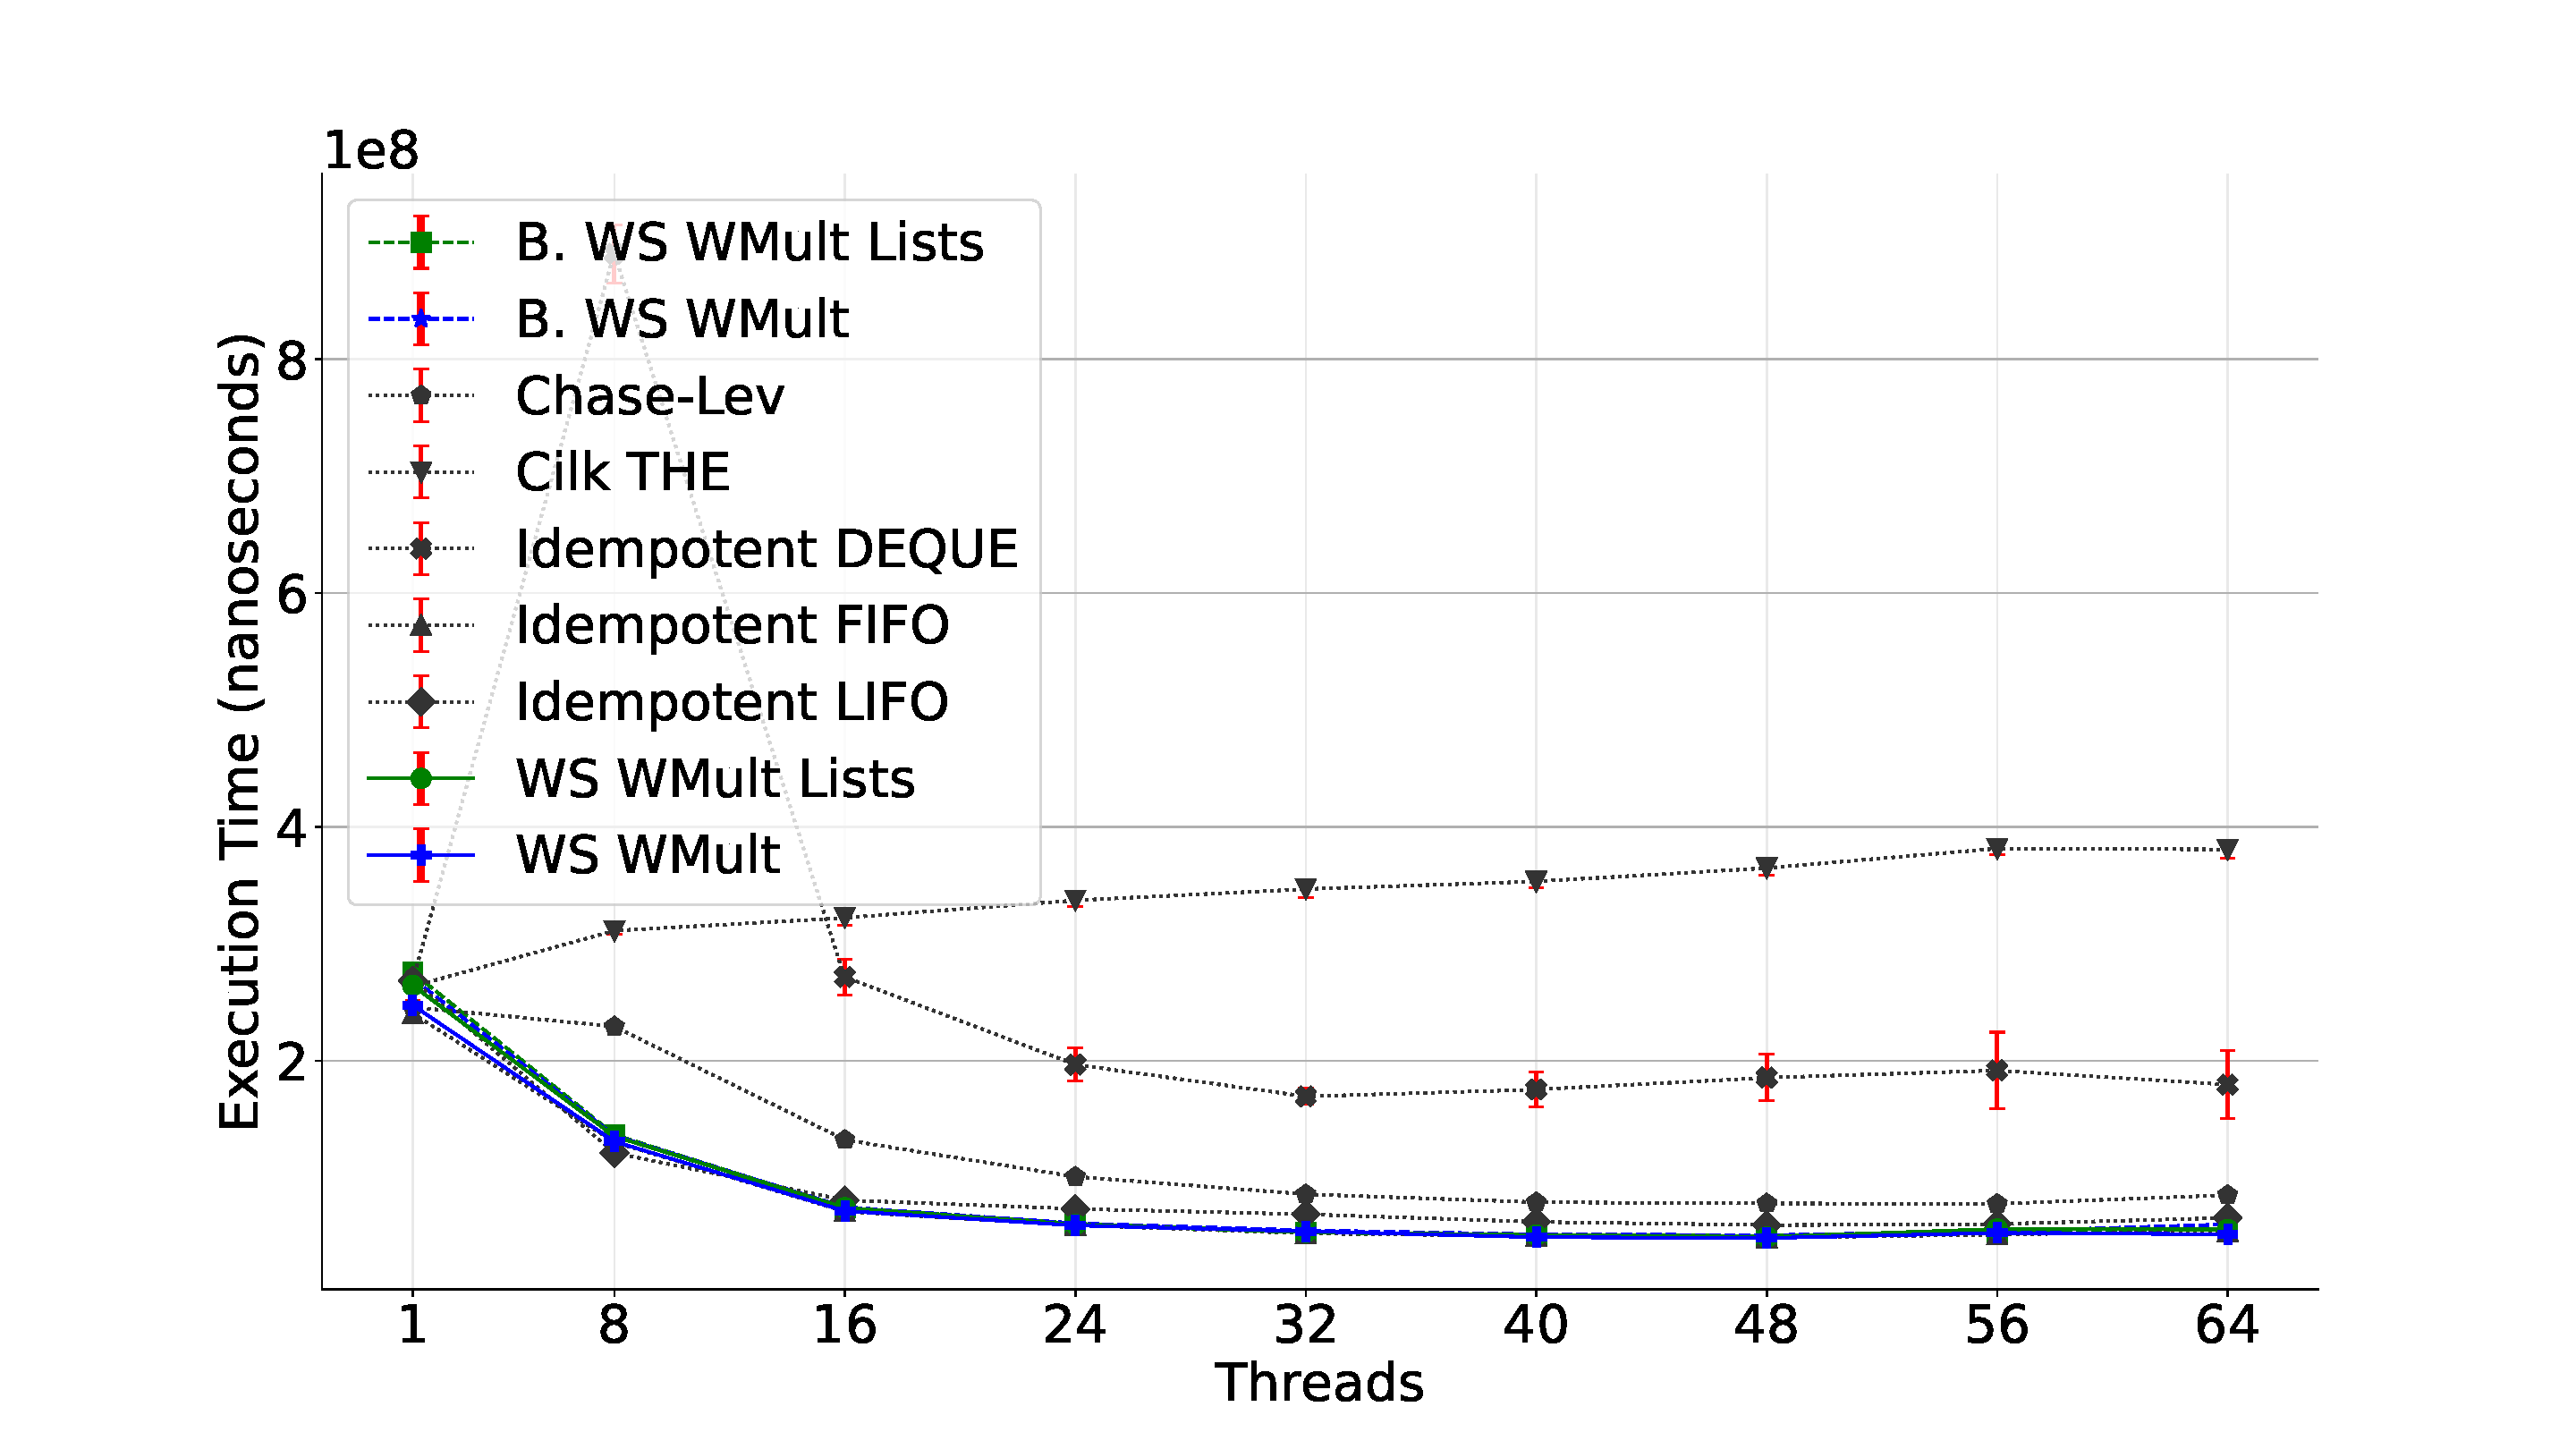
\includegraphics[width=0.48\textwidth]{contents/backmatter/evaluation/mean-TORUS2D-Directed-256.pdf}
  }
  \qquad
  \subfloat[\label{fig:directed_torus2d_1M} Mean times for the graph
  application benchmark. These are the results for the 2D Torus
  Directed graph. For each work-stealing algorithm's data structure,
  it begins its execution with an initial size of 1,000,000 entries.] {
    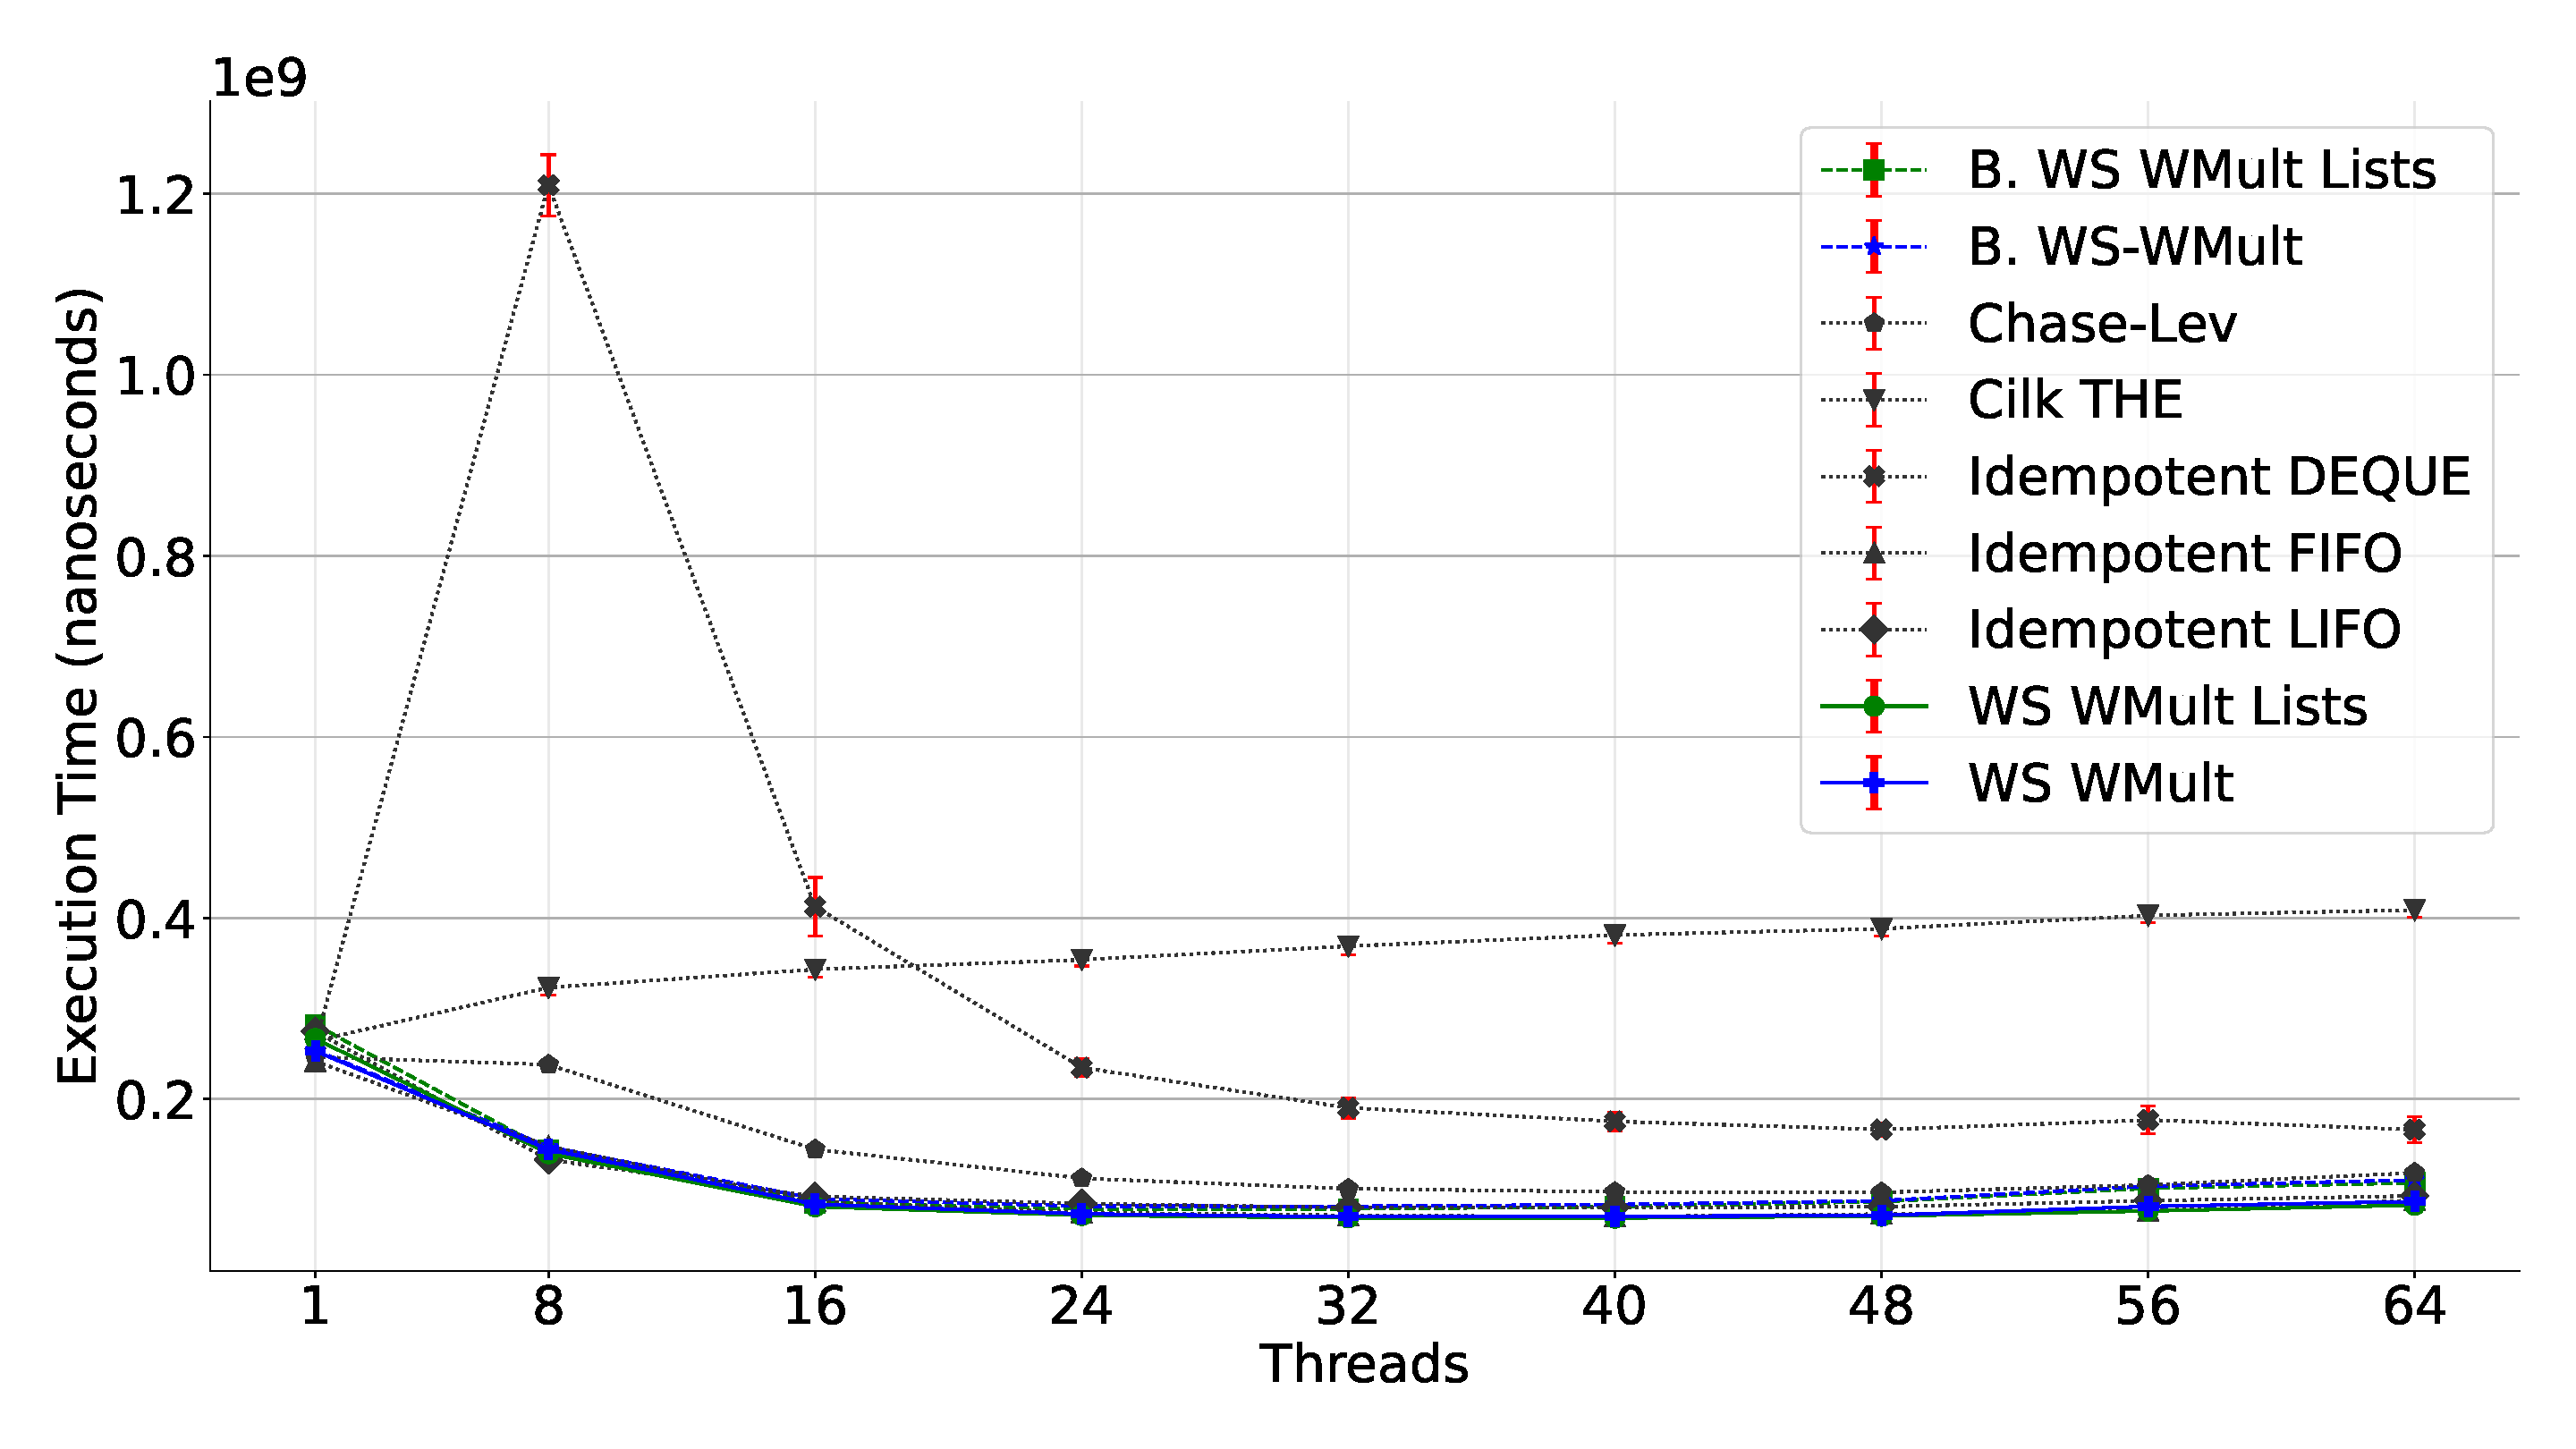
\includegraphics[width=0.48\textwidth]{contents/backmatter/evaluation/mean-TORUS2D-Directed-1000000.pdf}
  }

  \subfloat[\label{fig:undirected_torus2d_256} Mean times for the graph
  application benchmark. These are the results for the 2D Torus
  Undirected graph. For each work-stealing algorithm's data structure,
  it begins its execution with an initial size of 256 entries.] {
    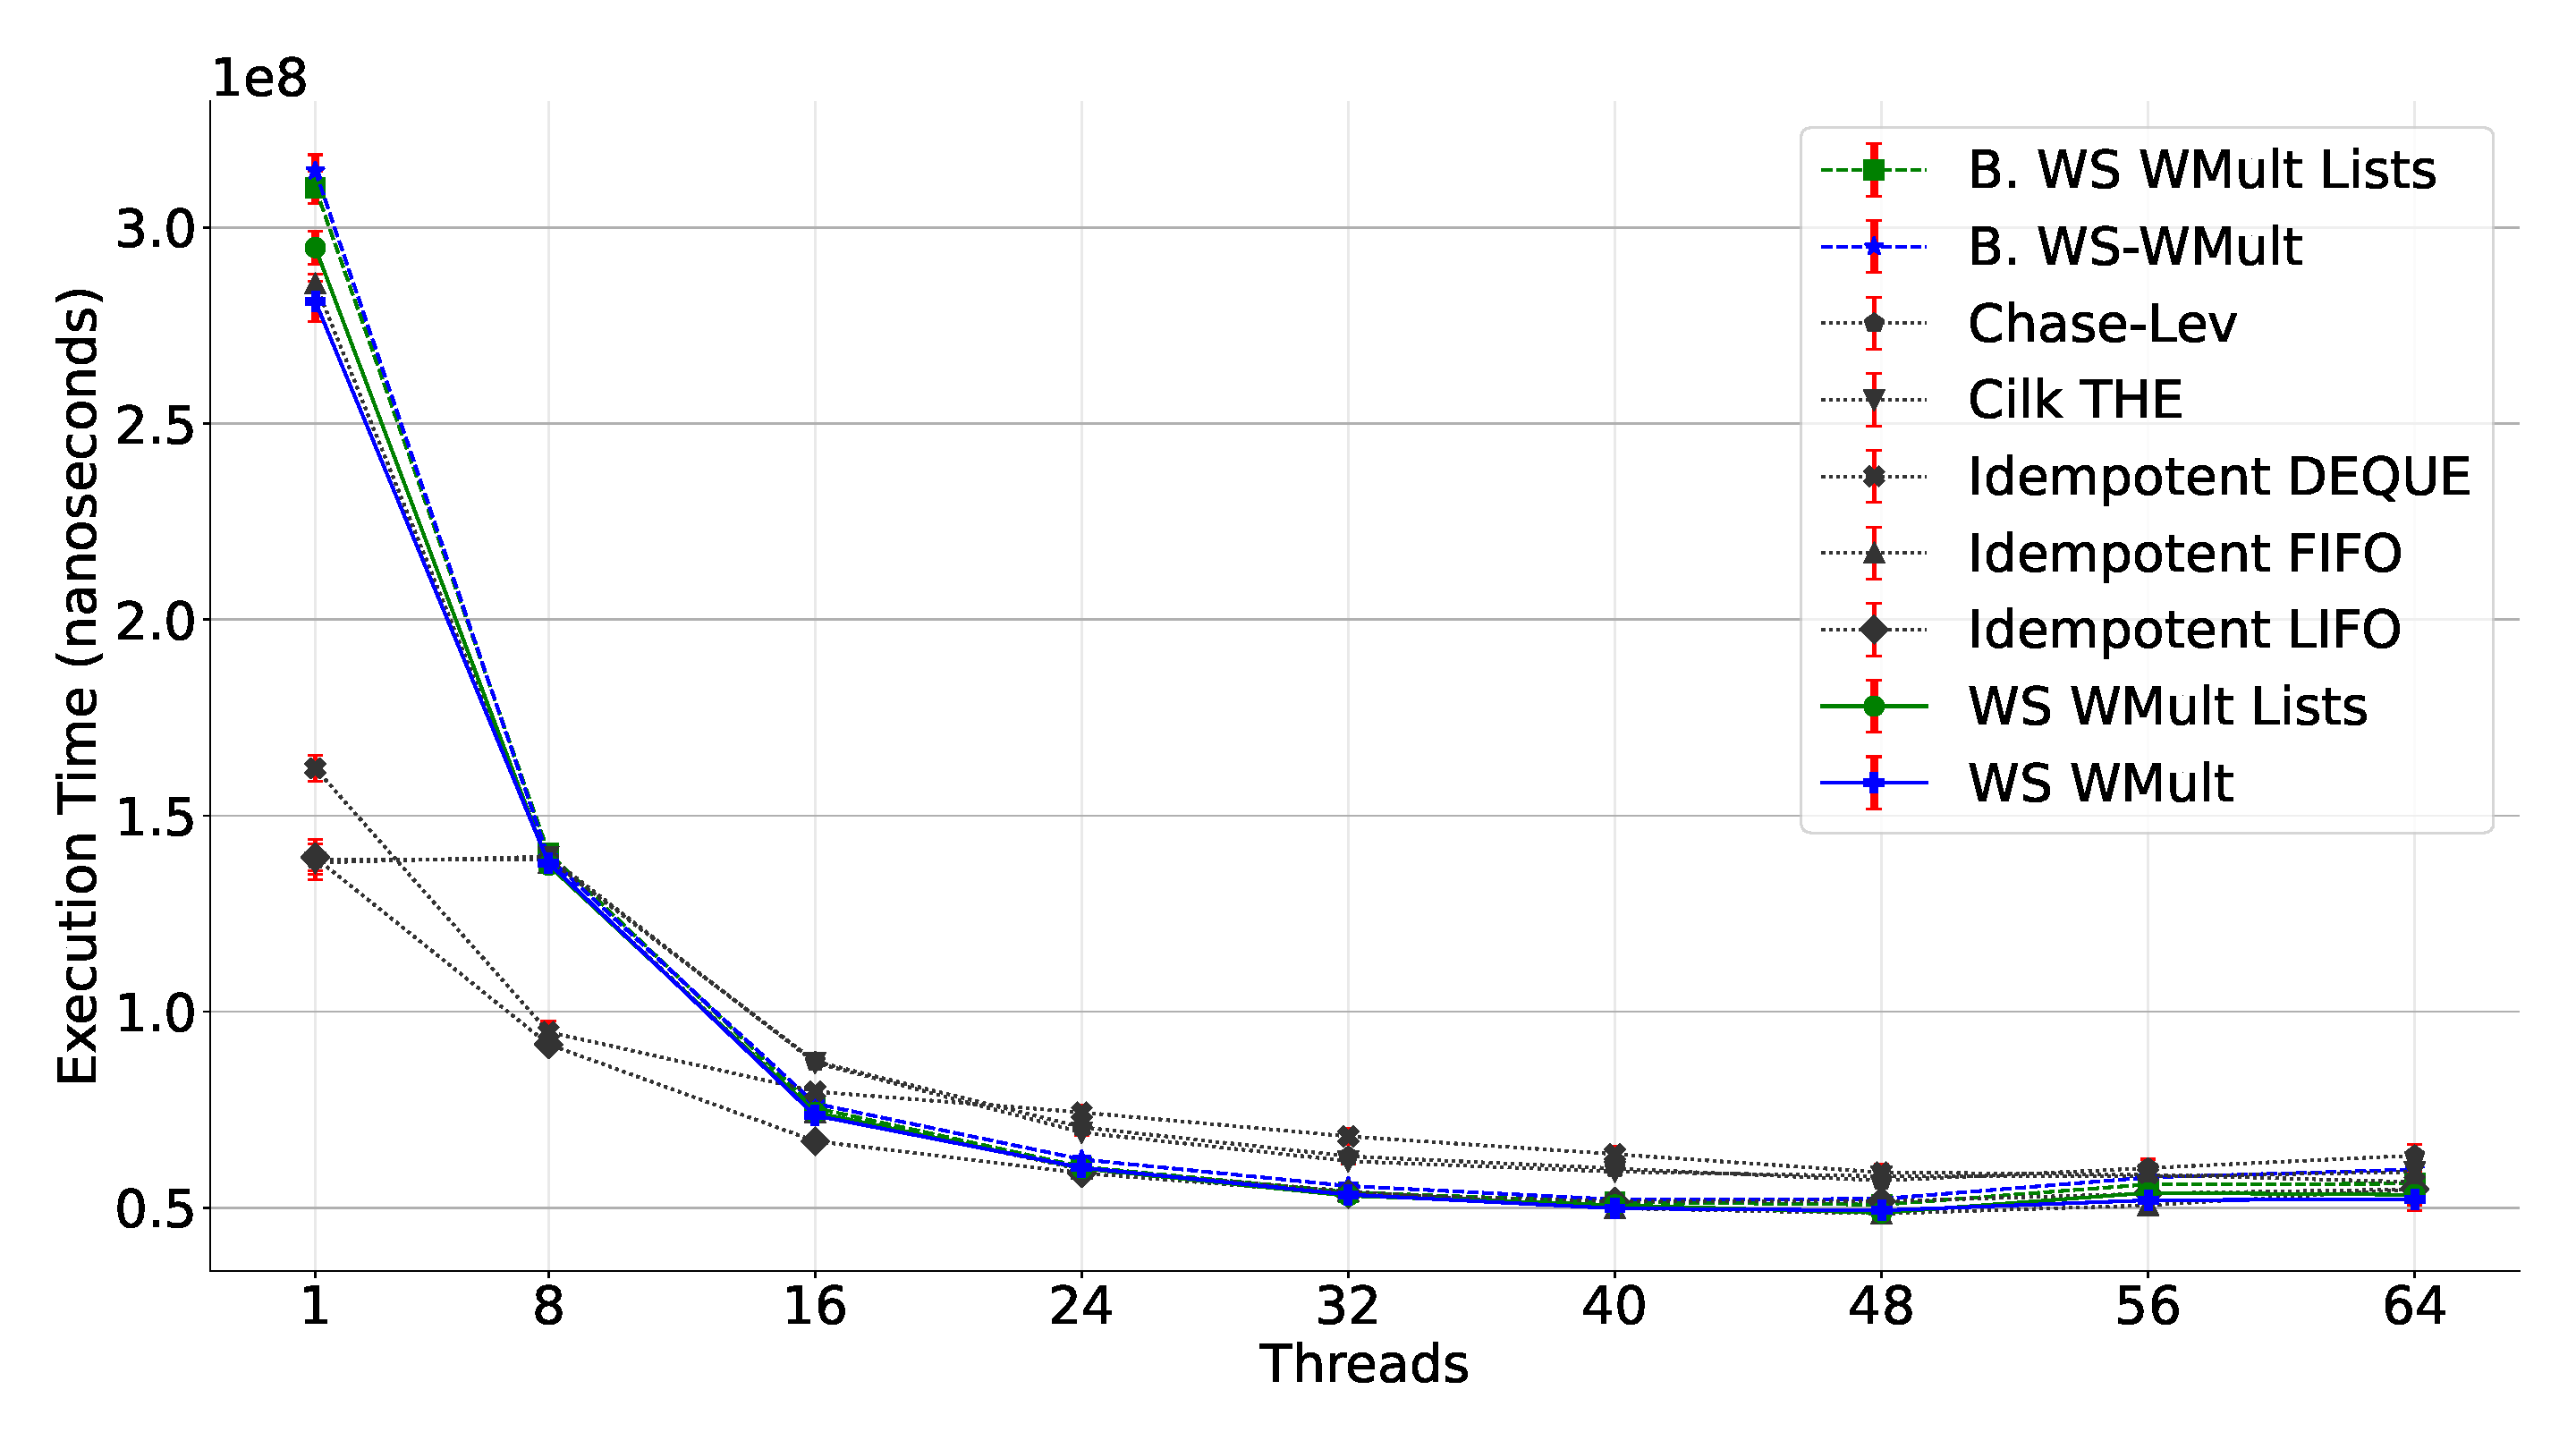
\includegraphics[width=0.48\textwidth]{contents/backmatter/evaluation/mean-TORUS2D-Undirected-256.pdf}
  }
  \qquad
  \subfloat[\label{fig:undirected_torus2d-1M} Mean times for the graph
  application benchmark. These are the results for the 2D Torus
  Undirected graph. For each work-stealing algorithm's
  data structure, it begins its execution with an initial size of
  1,000,000 entries.] {
    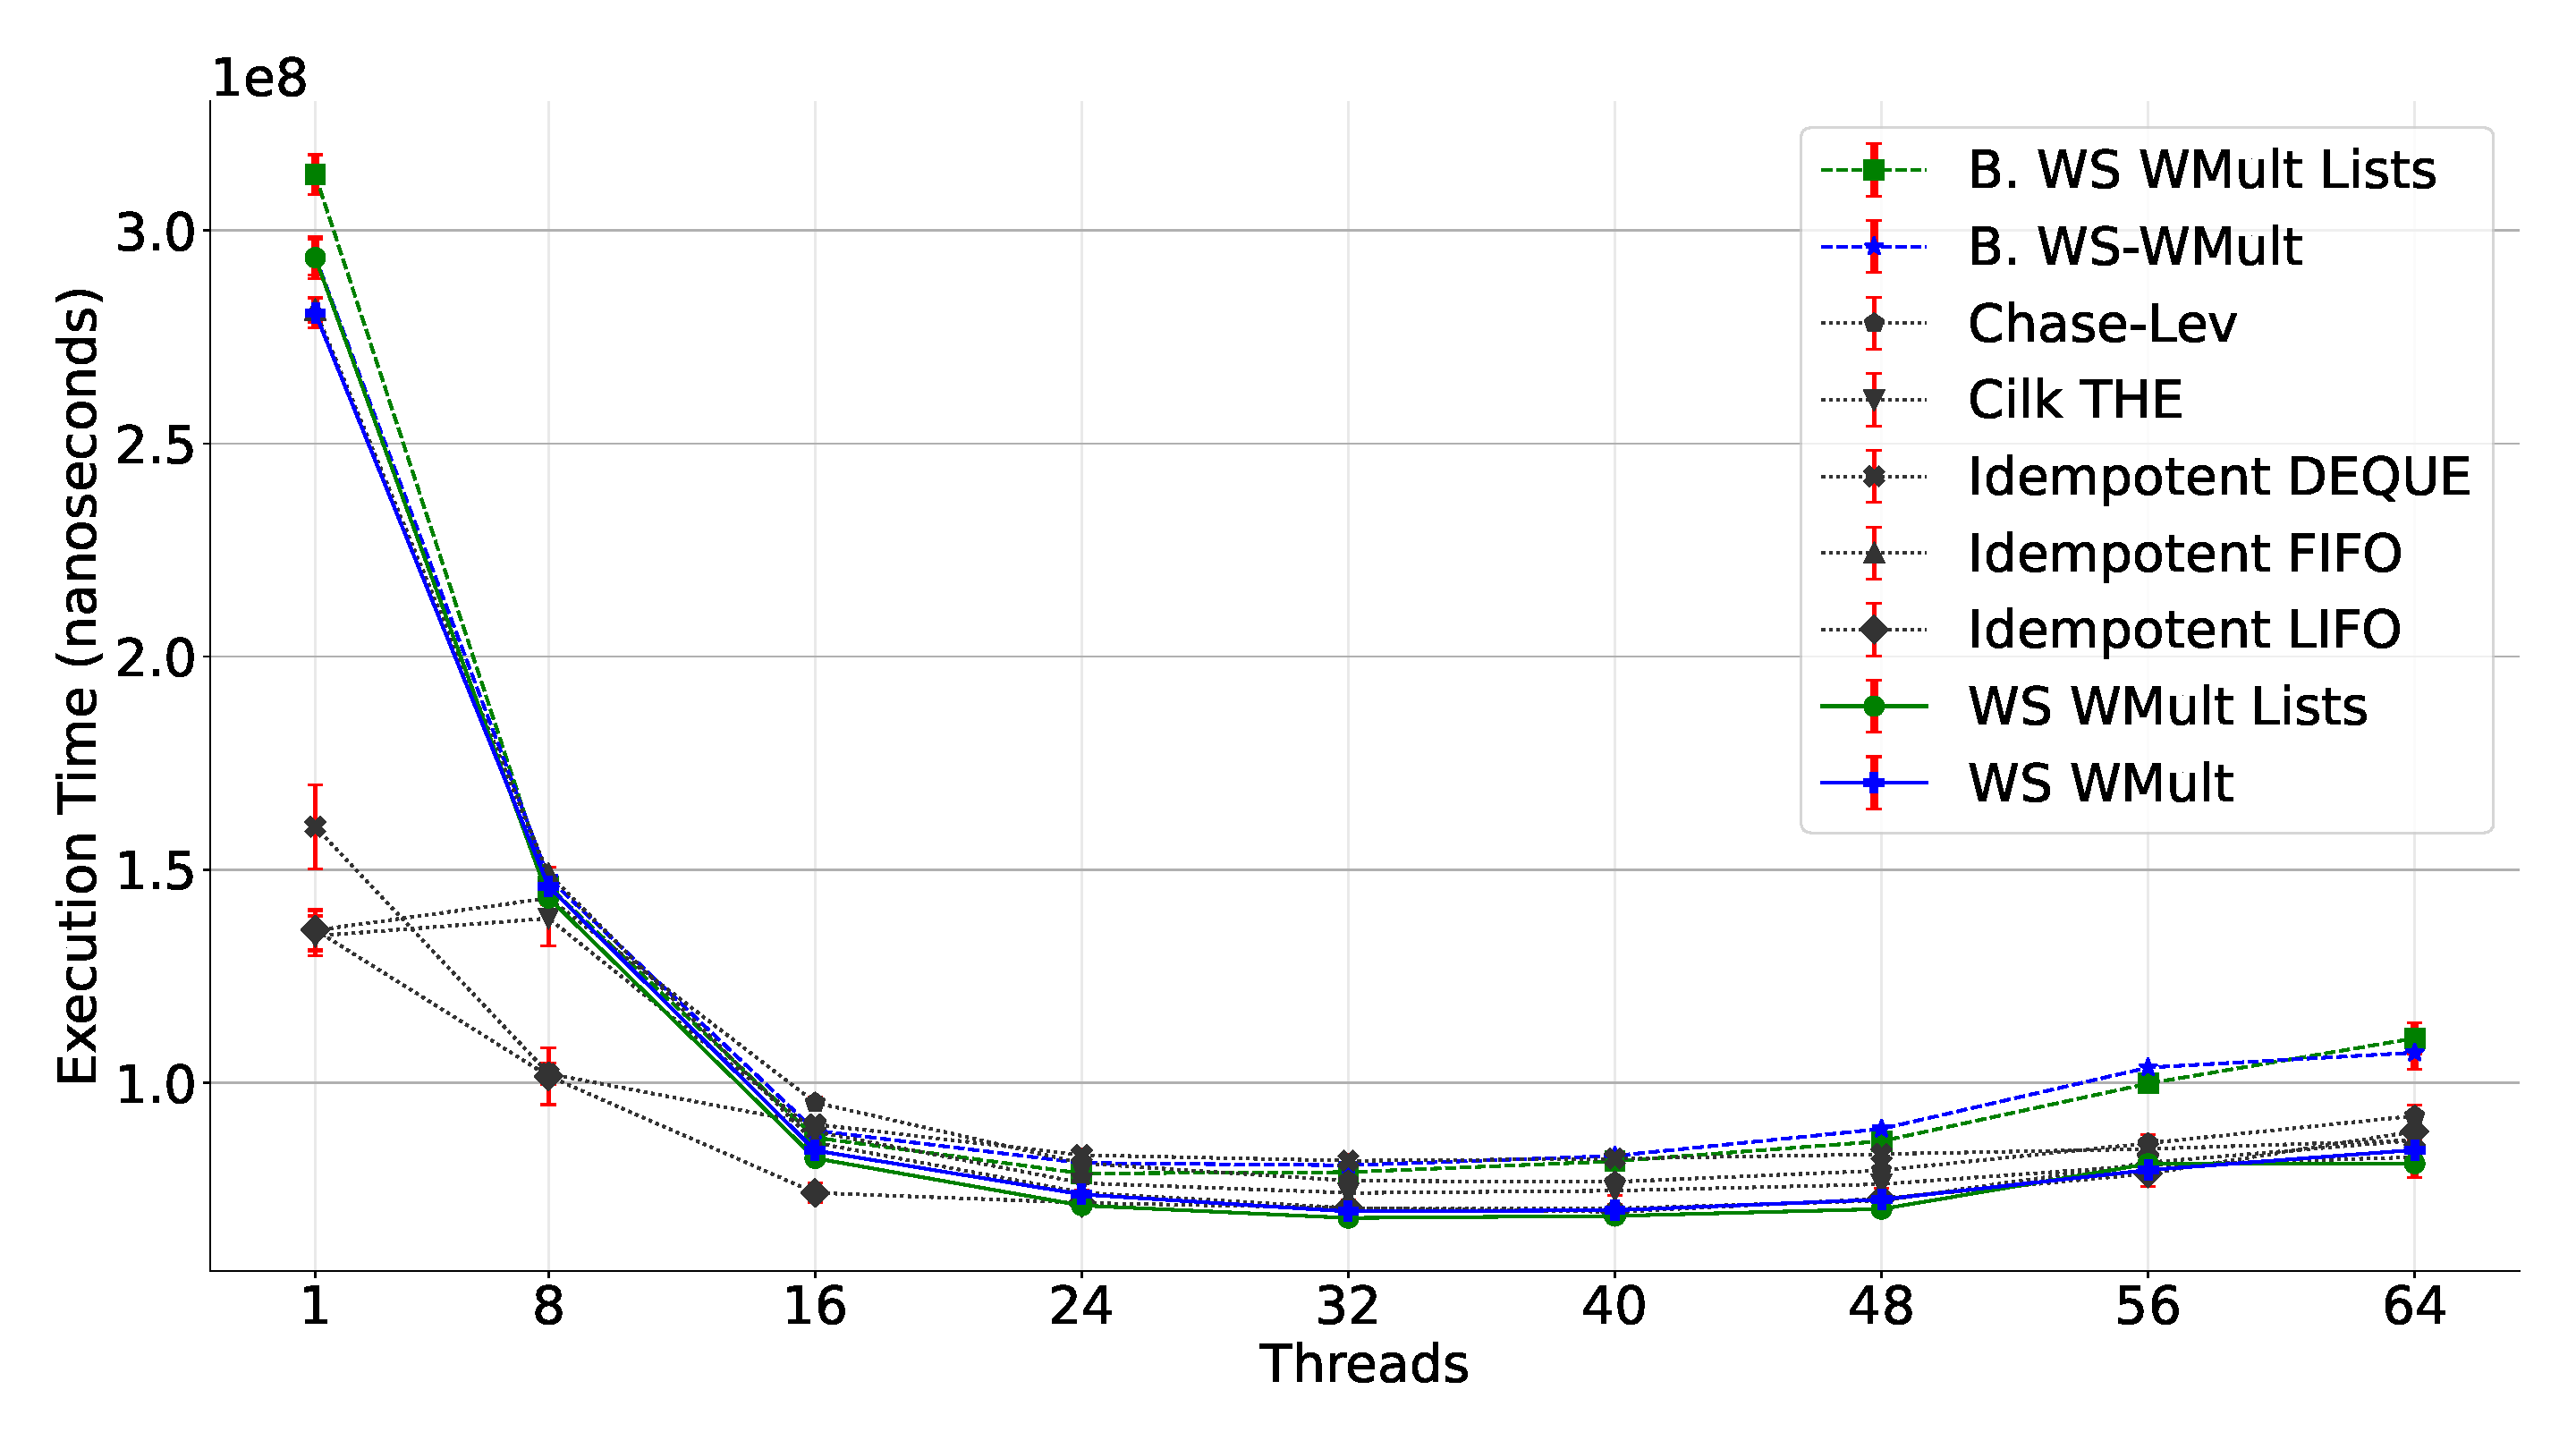
\includegraphics[width=0.48\textwidth]{contents/backmatter/evaluation/mean-TORUS2D-Undirected-1000000.pdf}
  }
  \caption{\label{fig:2d_torus_appendix} 2D Torus Directed and
    Undirected Graph with 256 and 1,000,000 initial sizes respectively.}
\end{figure}

\begin{table}[!ht]
\centering
\resizebox{\textwidth}{!}{\begin{tabular}{lrrrrrrrrr}
\toprule{} &           1  &           8  &           16 &           24 &           32 &           40 &           48 &           56 &           64 \\
\midrule
\textbf{B. WS WMult Lists} & 275477463.00 & 136788862.74 &  74324477.77 &  60730736.43 &  53505251.35 &  50743232.51 &  50292847.11 &  54089550.83 &  56234022.28 \\
\textbf{B. WS WMult      } & 270377949.90 & 135945596.35 &  74881098.84 &  61011775.05 &  55033500.39 &  51617389.18 &  50911385.25 &  54141726.30 &  60230204.70 \\
\textbf{Chase-Lev        } & 245820345.21 & 229356624.44 & 132371426.13 & 100919202.73 &  85931100.37 &  79043201.15 &  78056439.48 &  77733696.92 &  85279360.99 \\
\textbf{Cilk THE         } & 263677364.18 & 311281988.58 & 322321281.34 & 337196064.37 & 346876936.91 & 353384223.55 & 364851039.81 & 381583332.07 & 380634053.09 \\
\textbf{Idempotent DEQUE } & 268351478.04 & 890041843.06 & 271731282.68 & 196719701.28 & 169542956.14 & 175498130.08 & 185603584.54 & 191766131.46 & 179564368.52 \\
\textbf{Idempotent FIFO  } & 240555867.99 & 130412115.53 &  71135466.76 &  59469052.26 &  52425282.13 &  50053083.46 &  48699445.66 &  51530675.32 &  54082623.12 \\
\textbf{Idempotent LIFO  } & 268557944.01 & 121240023.29 &  80842396.35 &  73393176.30 &  68756656.08 &  62265055.27 &  59531339.13 &  60499769.67 &  65800153.04 \\
\textbf{WS WMult Lists   } & 264386117.47 & 135442458.17 &  74359990.60 &  60075063.34 &  53356451.31 &  51045223.01 &  49362511.61 &  56191157.64 &  55810986.14 \\
\textbf{WS WMult         } & 247514986.11 & 130992091.43 &  71628084.25 &  59275666.19 &  54259775.64 &  49197376.25 &  48457494.80 &  52845091.43 &  51699244.96 \\
\bottomrule
\end{tabular}}
\caption{Mean times for the graph application
    benchmark. These are the results for the 2D Torus Directed graph. Each
    algorithm begin its execution with an initial size of 256
    items.}
\label{graph-TORUS2D-Directed-256}
\end{table}

\begin{table}[!ht]
\centering
\resizebox{\textwidth}{!}{\begin{tabular}{lrrrrrrrrr}
\toprule{} &           1  &            8  &           16 &           24 &           32 &           40 &           48 &           56 &           64 \\
\midrule
\textbf{B. WS WMult Lists} & 282032101.13 &  143069494.72 &  85534815.94 &  78504149.89 &  78699282.75 &  81141869.21 &  86677012.58 & 101372180.23 & 107427536.39 \\
\textbf{B. W WMult      } & 254029656.93 &  147059256.57 &  89875139.77 &  81711438.58 &  81440512.00 &  83371685.71 &  87706342.83 & 103781818.41 & 110569292.18 \\
\textbf{Chase-Lev        } & 246442791.95 &  237923122.57 & 144322166.44 & 112347776.21 & 100841004.28 &  97312919.02 &  96845768.48 & 105140083.88 & 118527697.40 \\
\textbf{Cilk THE         } & 264300653.34 &  323239004.94 & 343356947.48 & 354030678.14 & 368922285.60 & 381228576.03 & 388191674.43 & 402911552.15 & 408918000.97 \\
\textbf{Idempotent DEQUE } & 260815108.20 & 1209548909.30 & 412614106.02 & 234745065.18 & 190273084.36 & 175218721.12 & 166271433.10 & 176938712.66 & 166152657.38 \\
\textbf{Idempotent FIFO  } & 241691715.81 &  147779277.84 &  86794723.48 &  74580951.70 &  71319113.57 &  69953403.69 &  72951557.67 &  76481707.91 &  88300511.33 \\
\textbf{Idempotent LIFO  } & 274669968.74 &  132876867.01 &  92359758.62 &  84527174.06 &  80000747.41 &  79918156.55 &  81057426.41 &  87742754.73 &  93122905.36 \\
\textbf{WS WMult Lists   } & 266732948.81 &  139727360.22 &  81166332.81 &  71537631.71 &  68838660.20 &  68622394.33 &  70694380.57 &  76278304.11 &  82762680.50 \\
\textbf{WS WMult         } & 253102197.42 &  144215742.72 &  83755232.58 &  73098841.65 &  69905539.84 &  70307884.91 &  71467092.10 &  81326080.28 &  86772858.87 \\
\bottomrule
\end{tabular}}
\caption{\label{graph-TORUS2D-Directed-1000000}Mean times for the graph application
    benchmark. These are the results for the 2D Torus Directed graph. Each
    algorithm begins its execution with an initial size of 1000000
    items.}
\end{table}

\begin{table}[!ht]
\centering
\resizebox{\textwidth}{!}{\begin{tabular}{lrrrrrrrrr}
\toprule{} &           1  &           8  &          16 &          24 &          32 &          40 &          48 &          56 &          64 \\
\midrule
\textbf{B. WS WMult Lists} & 310159873.86 & 140439779.78 & 75432726.40 & 60406182.71 & 53911161.76 & 51430777.91 & 50753159.38 & 55951600.18 & 56137962.96 \\
\textbf{B. WS WMult      } & 314452637.35 & 139249013.63 & 76542543.20 & 62311010.87 & 55528149.56 & 52097619.34 & 52246241.13 & 57724836.67 & 59747465.26 \\
\textbf{Chase-Lev        } & 138828051.42 & 138897518.79 & 87292876.34 & 70522950.03 & 63105704.93 & 59978683.77 & 56908800.75 & 60120171.07 & 63348521.30 \\
\textbf{Cilk THE         } & 138028046.12 & 139574907.75 & 86992872.27 & 69182659.71 & 61861841.16 & 59163947.75 & 58000268.78 & 57943903.04 & 59164952.68 \\
\textbf{Idempotent DEQUE } & 162061744.20 &  94795698.28 & 79606910.26 & 74293432.40 & 68175669.64 & 63633505.52 & 59008790.10 & 58410327.72 & 56516387.48 \\
\textbf{Idempotent FIFO  } & 285722944.41 & 137771932.41 & 74313817.07 & 59775880.18 & 54199431.72 & 49858050.44 & 48473814.48 & 50603478.05 & 54748949.06 \\
\textbf{Idempotent LIFO  } & 139329399.29 &  91652023.21 & 66936992.03 & 58831954.84 & 53465545.93 & 51570670.85 & 51610279.19 & 53622297.77 & 54754410.32 \\
\textbf{WS WMult Lists   } & 294863903.34 & 137331873.11 & 74299658.78 & 60022488.79 & 53029369.50 & 50656621.07 & 48692765.58 & 53784545.47 & 53296961.05 \\
\textbf{WS WMult         } & 281148635.39 & 137928573.11 & 73505852.13 & 60207428.55 & 53334767.43 & 49825802.09 & 49308366.02 & 51896274.03 & 52172465.28 \\
\bottomrule
\end{tabular}}

\caption{\label{graph-TORUS2D-Undirected-256}Mean times for the graph application
    benchmark. These are the results for the 2D Torus Undirected graph. Each
    algorithm begins its execution with an initial size of 256
    items.}
\end{table}

\begin{table}[!ht]
\centering
\resizebox{\textwidth}{!}{\begin{tabular}{lrrrrrrrrr}
\toprule{} &           1  &           8  &          16 &          24 &          32 &          40 &          48 &           56 &           64 \\
\midrule
\textbf{B. WS WMult Lists} & 313137477.28 & 146059161.29 & 87094776.55 & 78679883.57 & 78976895.23 & 81553430.32 & 86244666.42 &  99783595.98 & 110398812.46 \\
\textbf{B. WS WMult      } & 293784827.34 & 147980221.95 & 88731594.96 & 81121304.79 & 80579591.88 & 82813668.25 & 89143510.85 & 103539594.14 & 107036269.51 \\
\textbf{Chase-Lev        } & 135739209.18 & 143310608.07 & 95323139.46 & 81052618.70 & 76940451.27 & 76699127.81 & 79395479.61 &  85791529.95 &  92214170.11 \\
\textbf{Cilk THE         } & 134426266.75 & 138584211.69 & 88507523.61 & 76405888.32 & 74084595.82 & 74632761.47 & 76161617.37 &  80595336.35 &  82538974.04 \\
\textbf{Idempotent DEQUE } & 160055984.00 & 102061319.64 & 90198138.78 & 82973638.50 & 81645834.10 & 82150883.36 & 83227444.86 &  84420556.12 &  86499396.64 \\
\textbf{Idempotent FIFO  } & 281355092.48 & 149030688.81 & 85883852.60 & 74176611.42 & 70542525.74 & 70451746.00 & 72308567.54 &  81236910.85 &  86493594.23 \\
\textbf{Idempotent LIFO  } & 135852779.09 & 101491242.31 & 74122390.31 & 71756053.52 & 70549755.43 & 69617711.32 & 72795329.85 &  78634423.92 &  88549939.13 \\
\textbf{WS WMult Lists   } & 293649514.77 & 143351585.30 & 82231696.72 & 71153322.35 & 68221248.95 & 68690573.69 & 70317039.66 &  80917247.72 &  81000767.24 \\
\textbf{WS WMult         } & 280609111.62 & 146014648.66 & 84057327.09 & 73737753.72 & 69754078.34 & 70027563.45 & 72554542.24 &  79464648.48 &  84181768.65 \\
\bottomrule
\end{tabular}}

\caption{\label{graph-TORUS2D-Undirected-1000000}Mean times for the graph application
    benchmark. These are the results for the 2D Torus Undirected graph. Each
    algorithm begins its execution with an initial size of 1000000
    items.}
\end{table}



\begin{figure}[!ht]
  \subfloat[\label{fig:directed_torus2d60_256}  Mean times for the graph
  application benchmark. These are the results of the 2D Torus 60\%
  Directed graph. For each work-stealing algorithm's
  data structure, it begins its execution with an initial size of
  256 entries.] {
    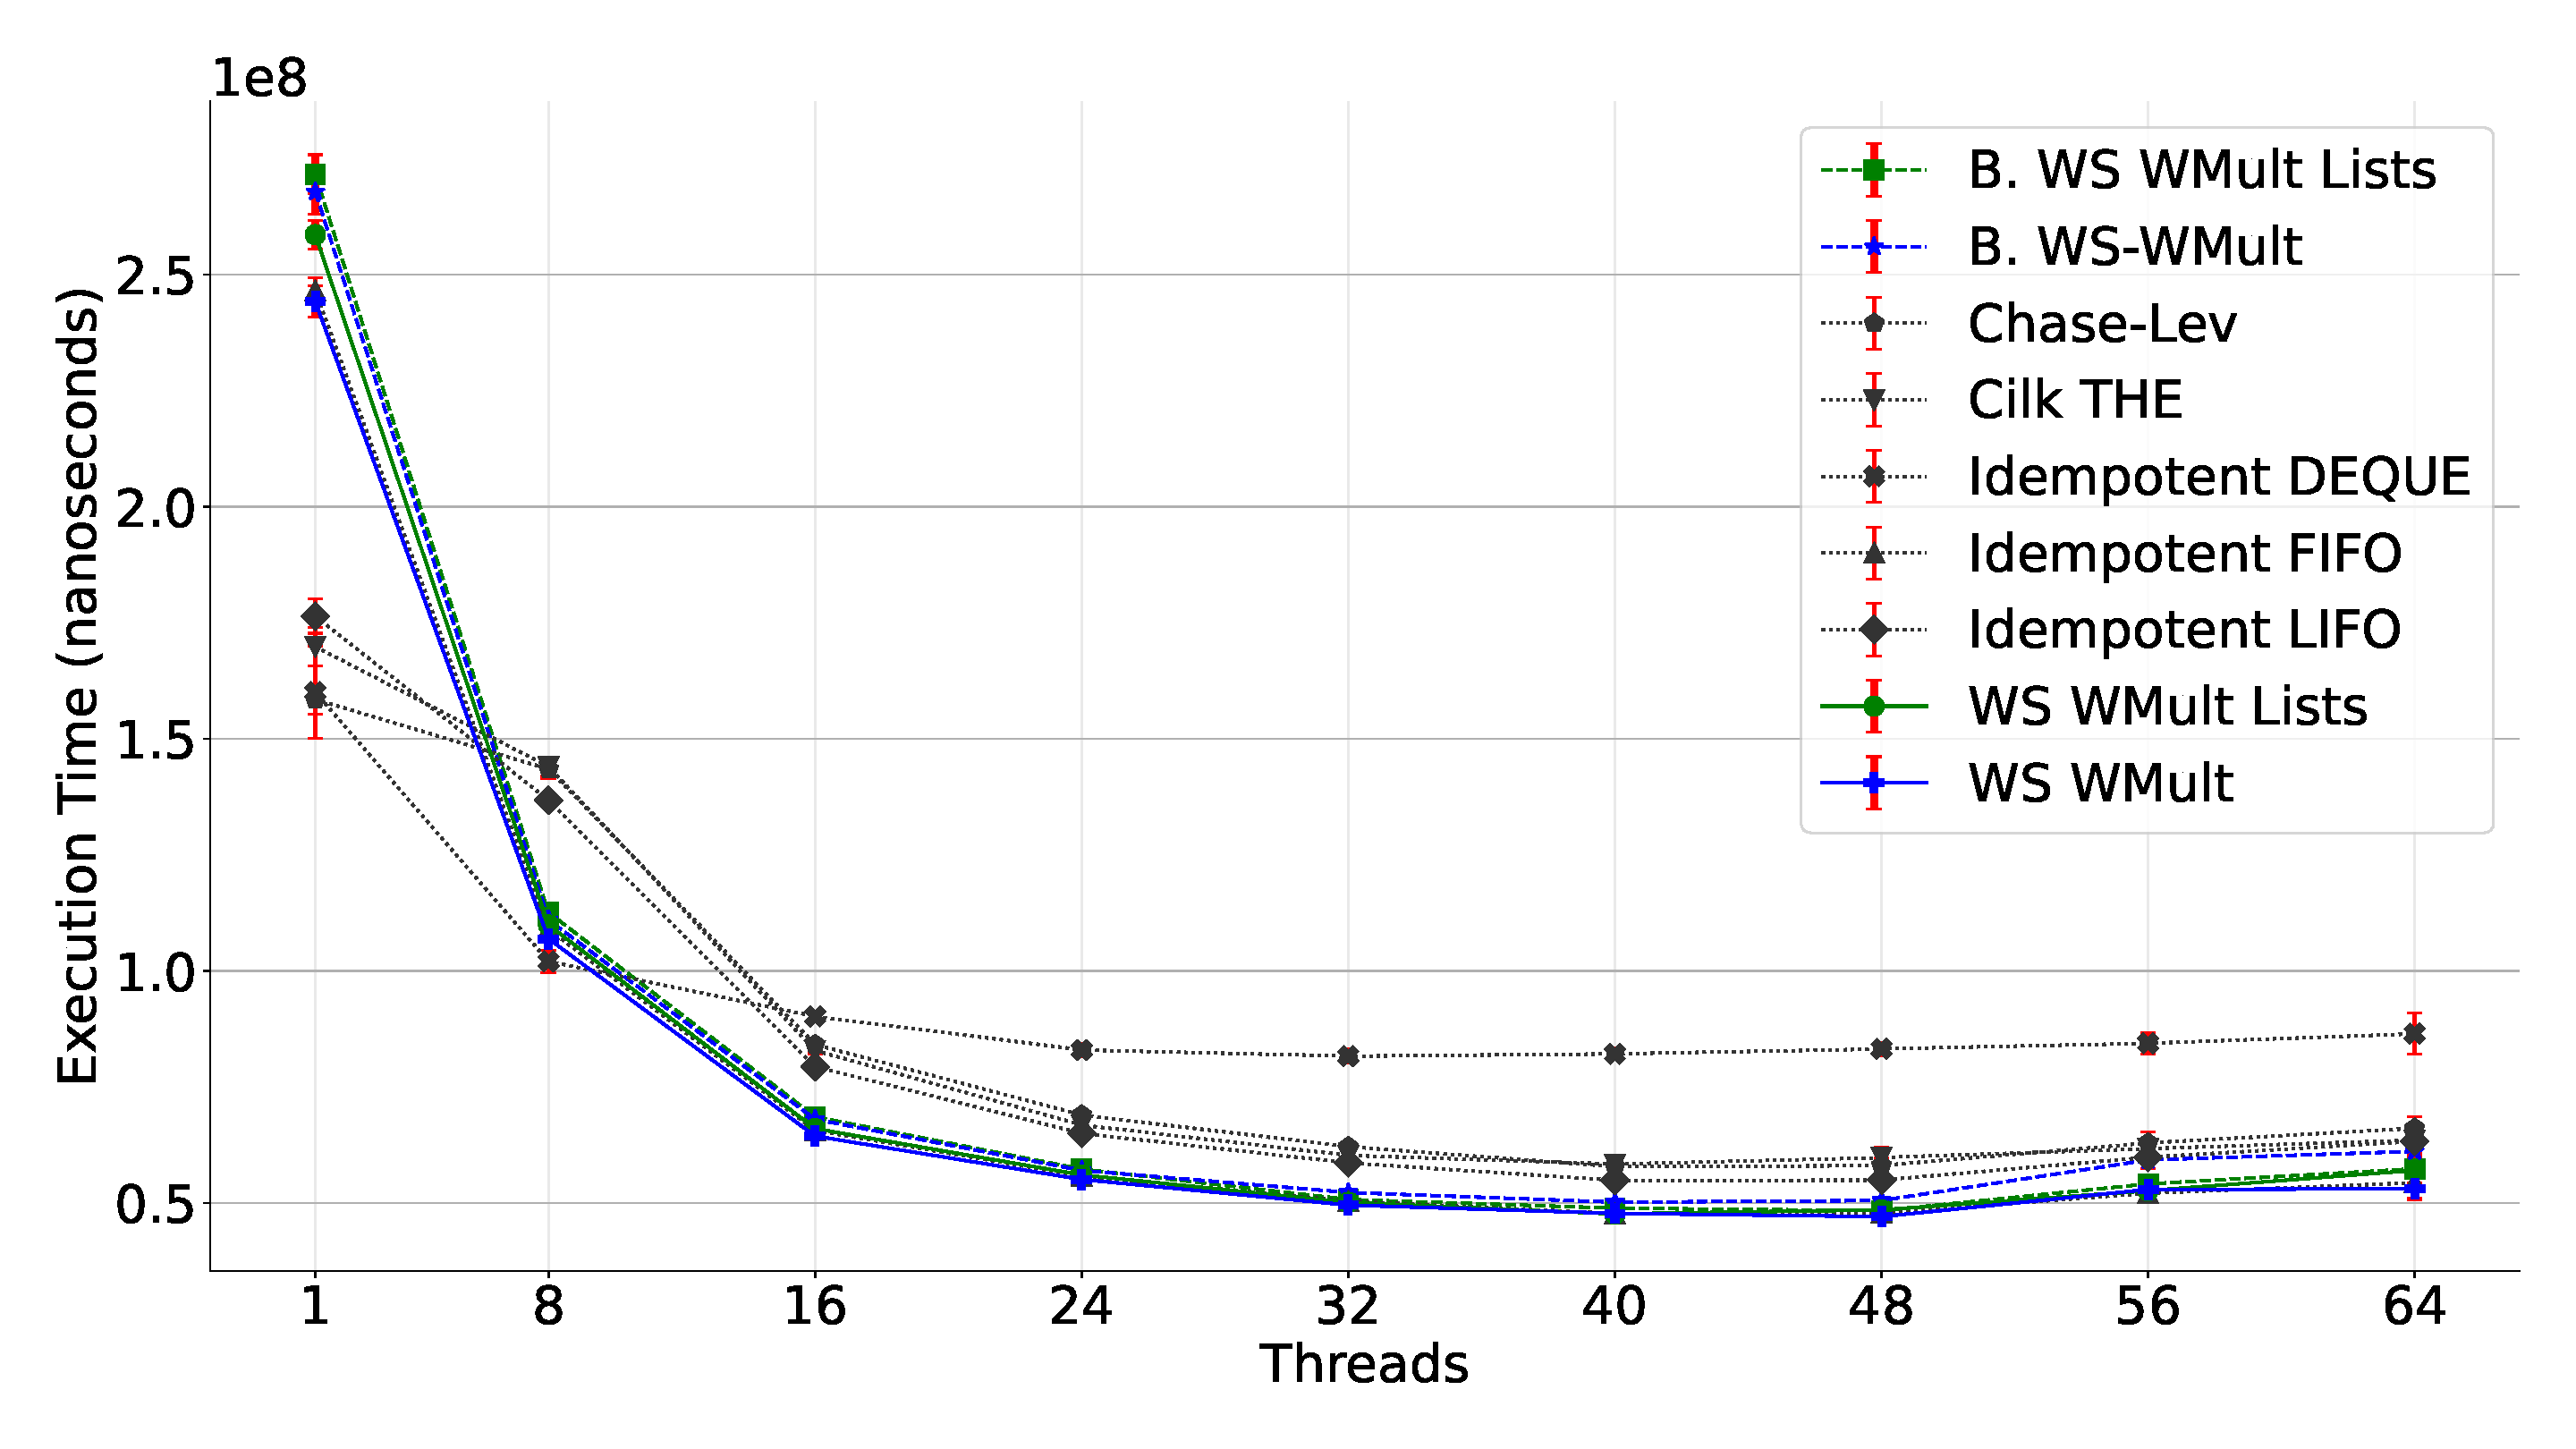
\includegraphics[width=0.48\textwidth]{contents/backmatter/evaluation/mean-TORUS2D60-Directed-256.pdf}
  }
  \qquad
  \subfloat[\label{fig:directed_torus2d60_1M} Mean times for the graph
  application benchmark. These are the results of the 2D Torus 60\%
  Directed graph. For each work-stealing algorithm's
  data structure, it begins its execution with an initial size of
  1,000,000 entries.] {
    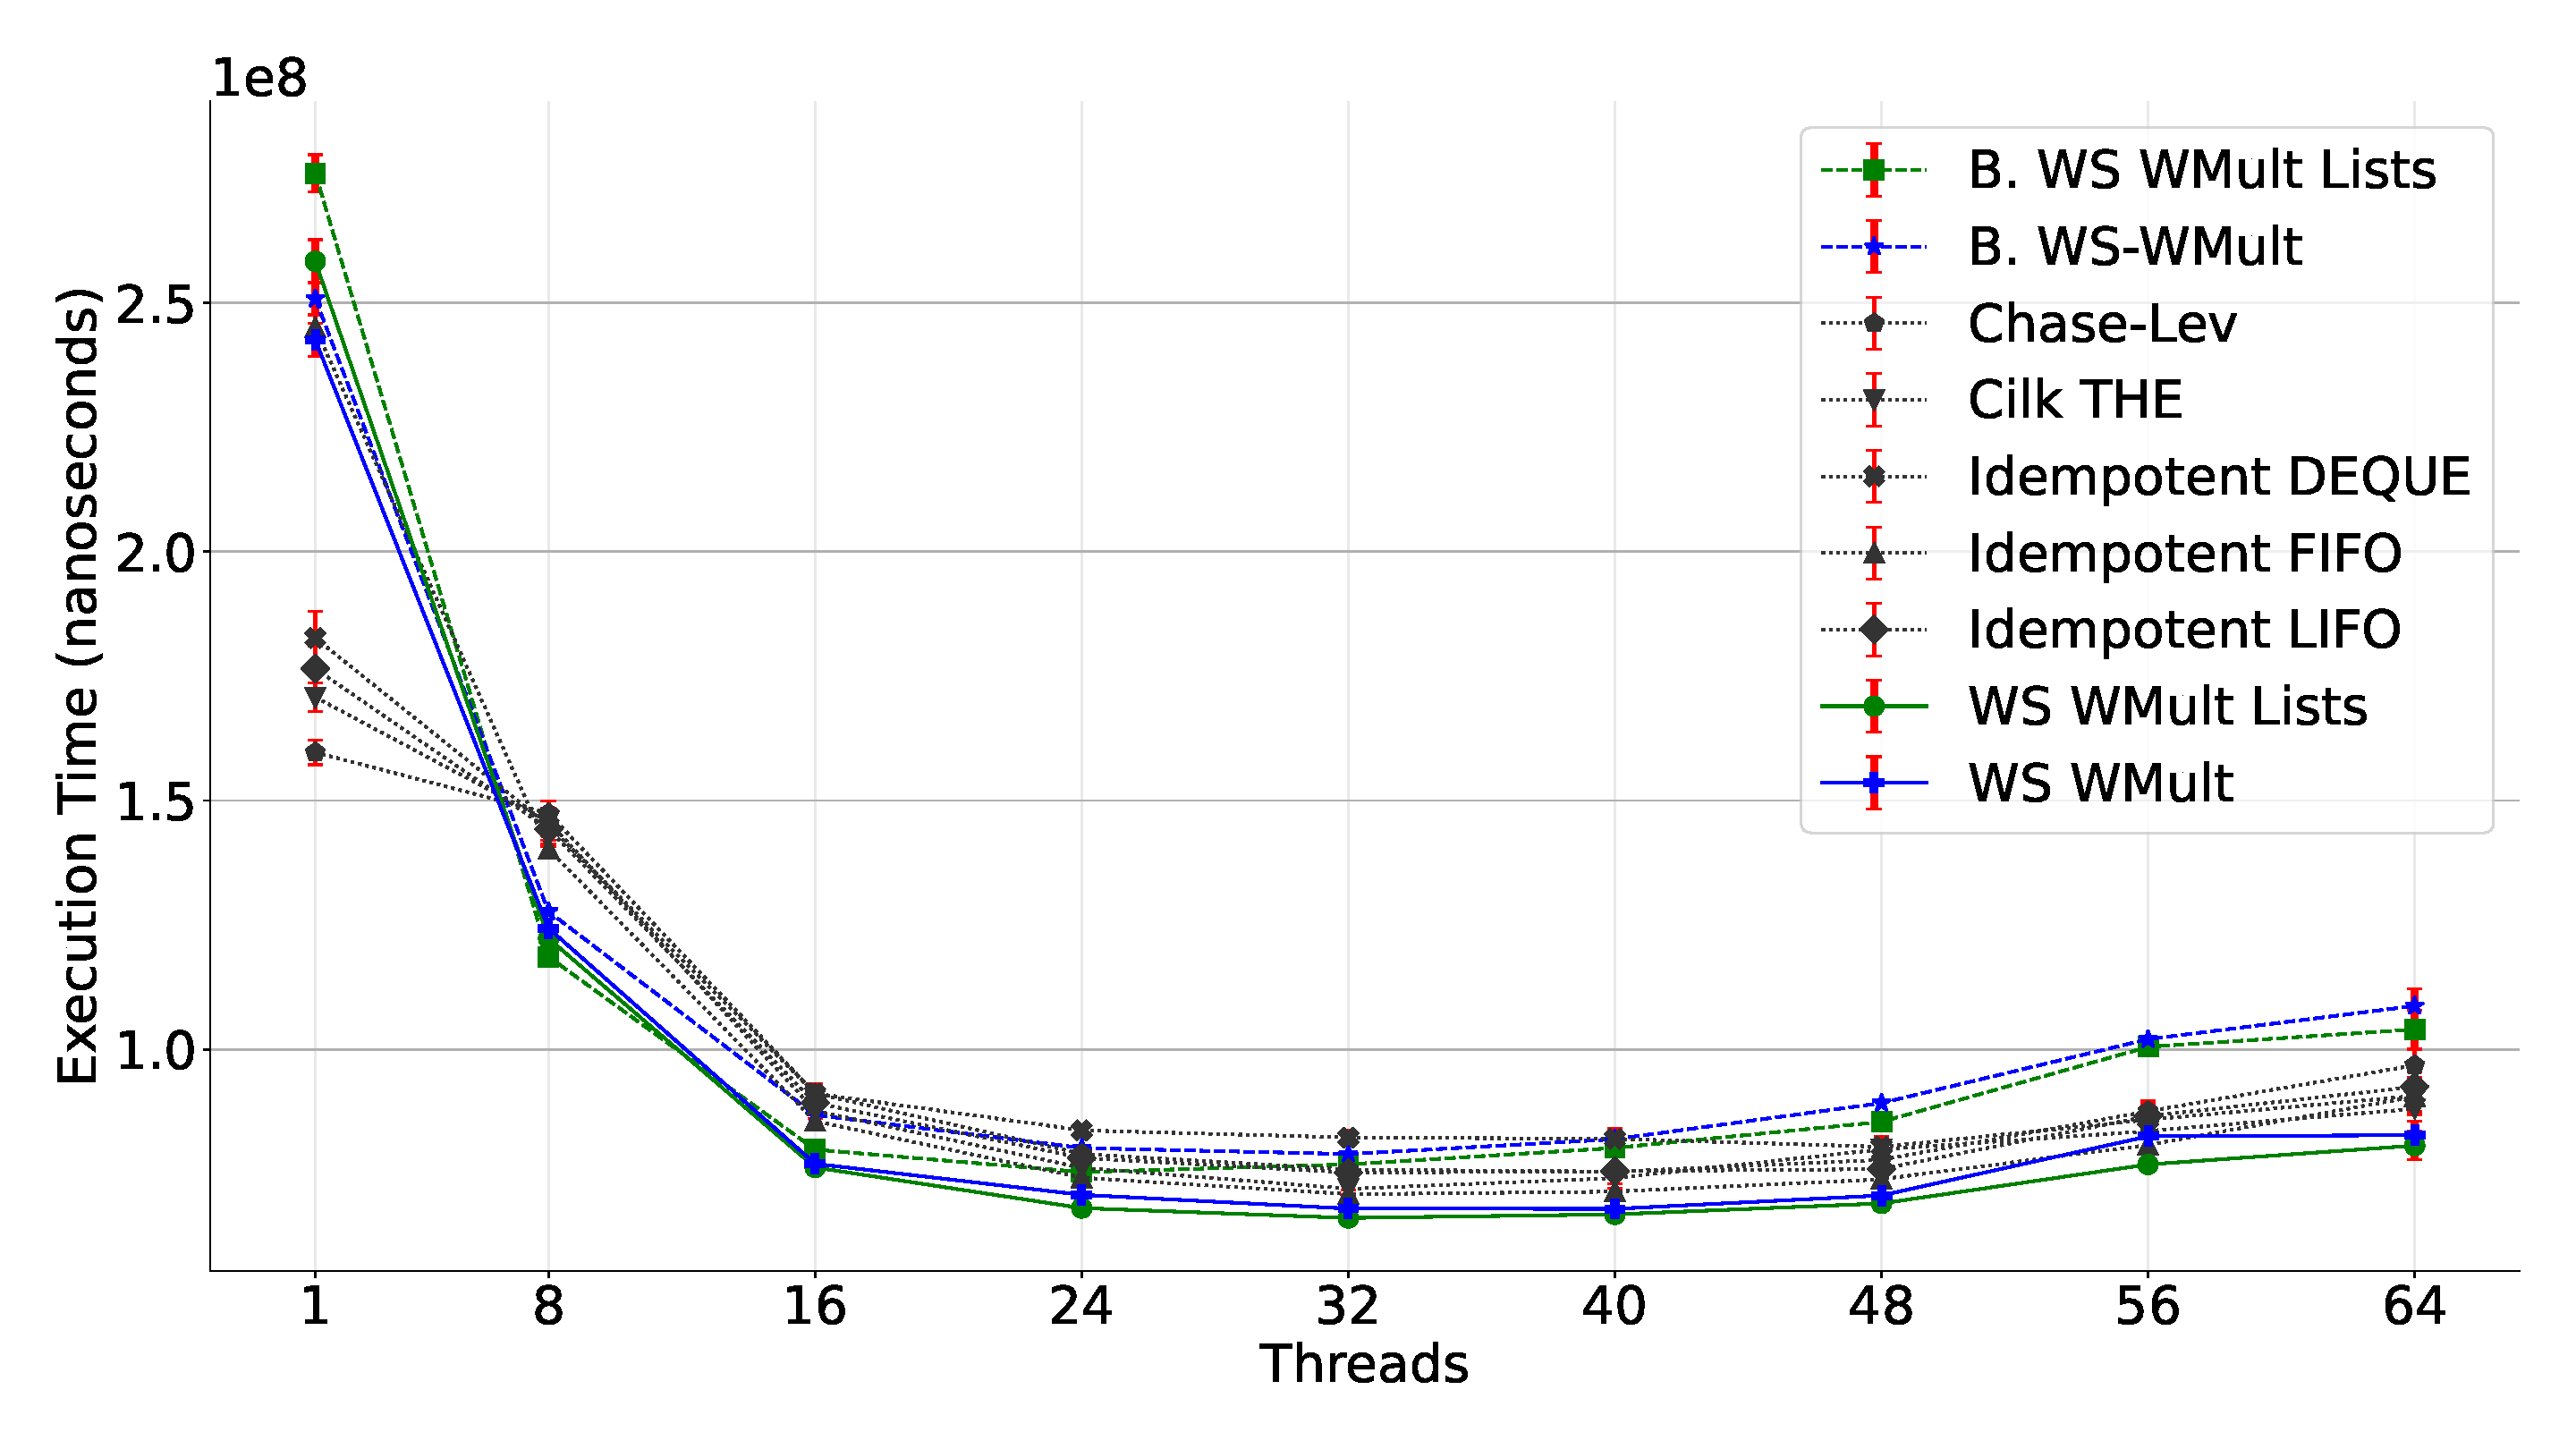
\includegraphics[width=0.48\textwidth]{contents/backmatter/evaluation/mean-TORUS2D60-Directed-1000000.pdf}
  }

  \subfloat[\label{fig:undirected_torus2d60_256} Mean times for the graph
  application benchmark. These are the results of the 2D Torus 60\%
  Undirected graph. For each work-stealing algorithm's
  data structure, it begins its execution with an initial size of
  256 entries.] {
    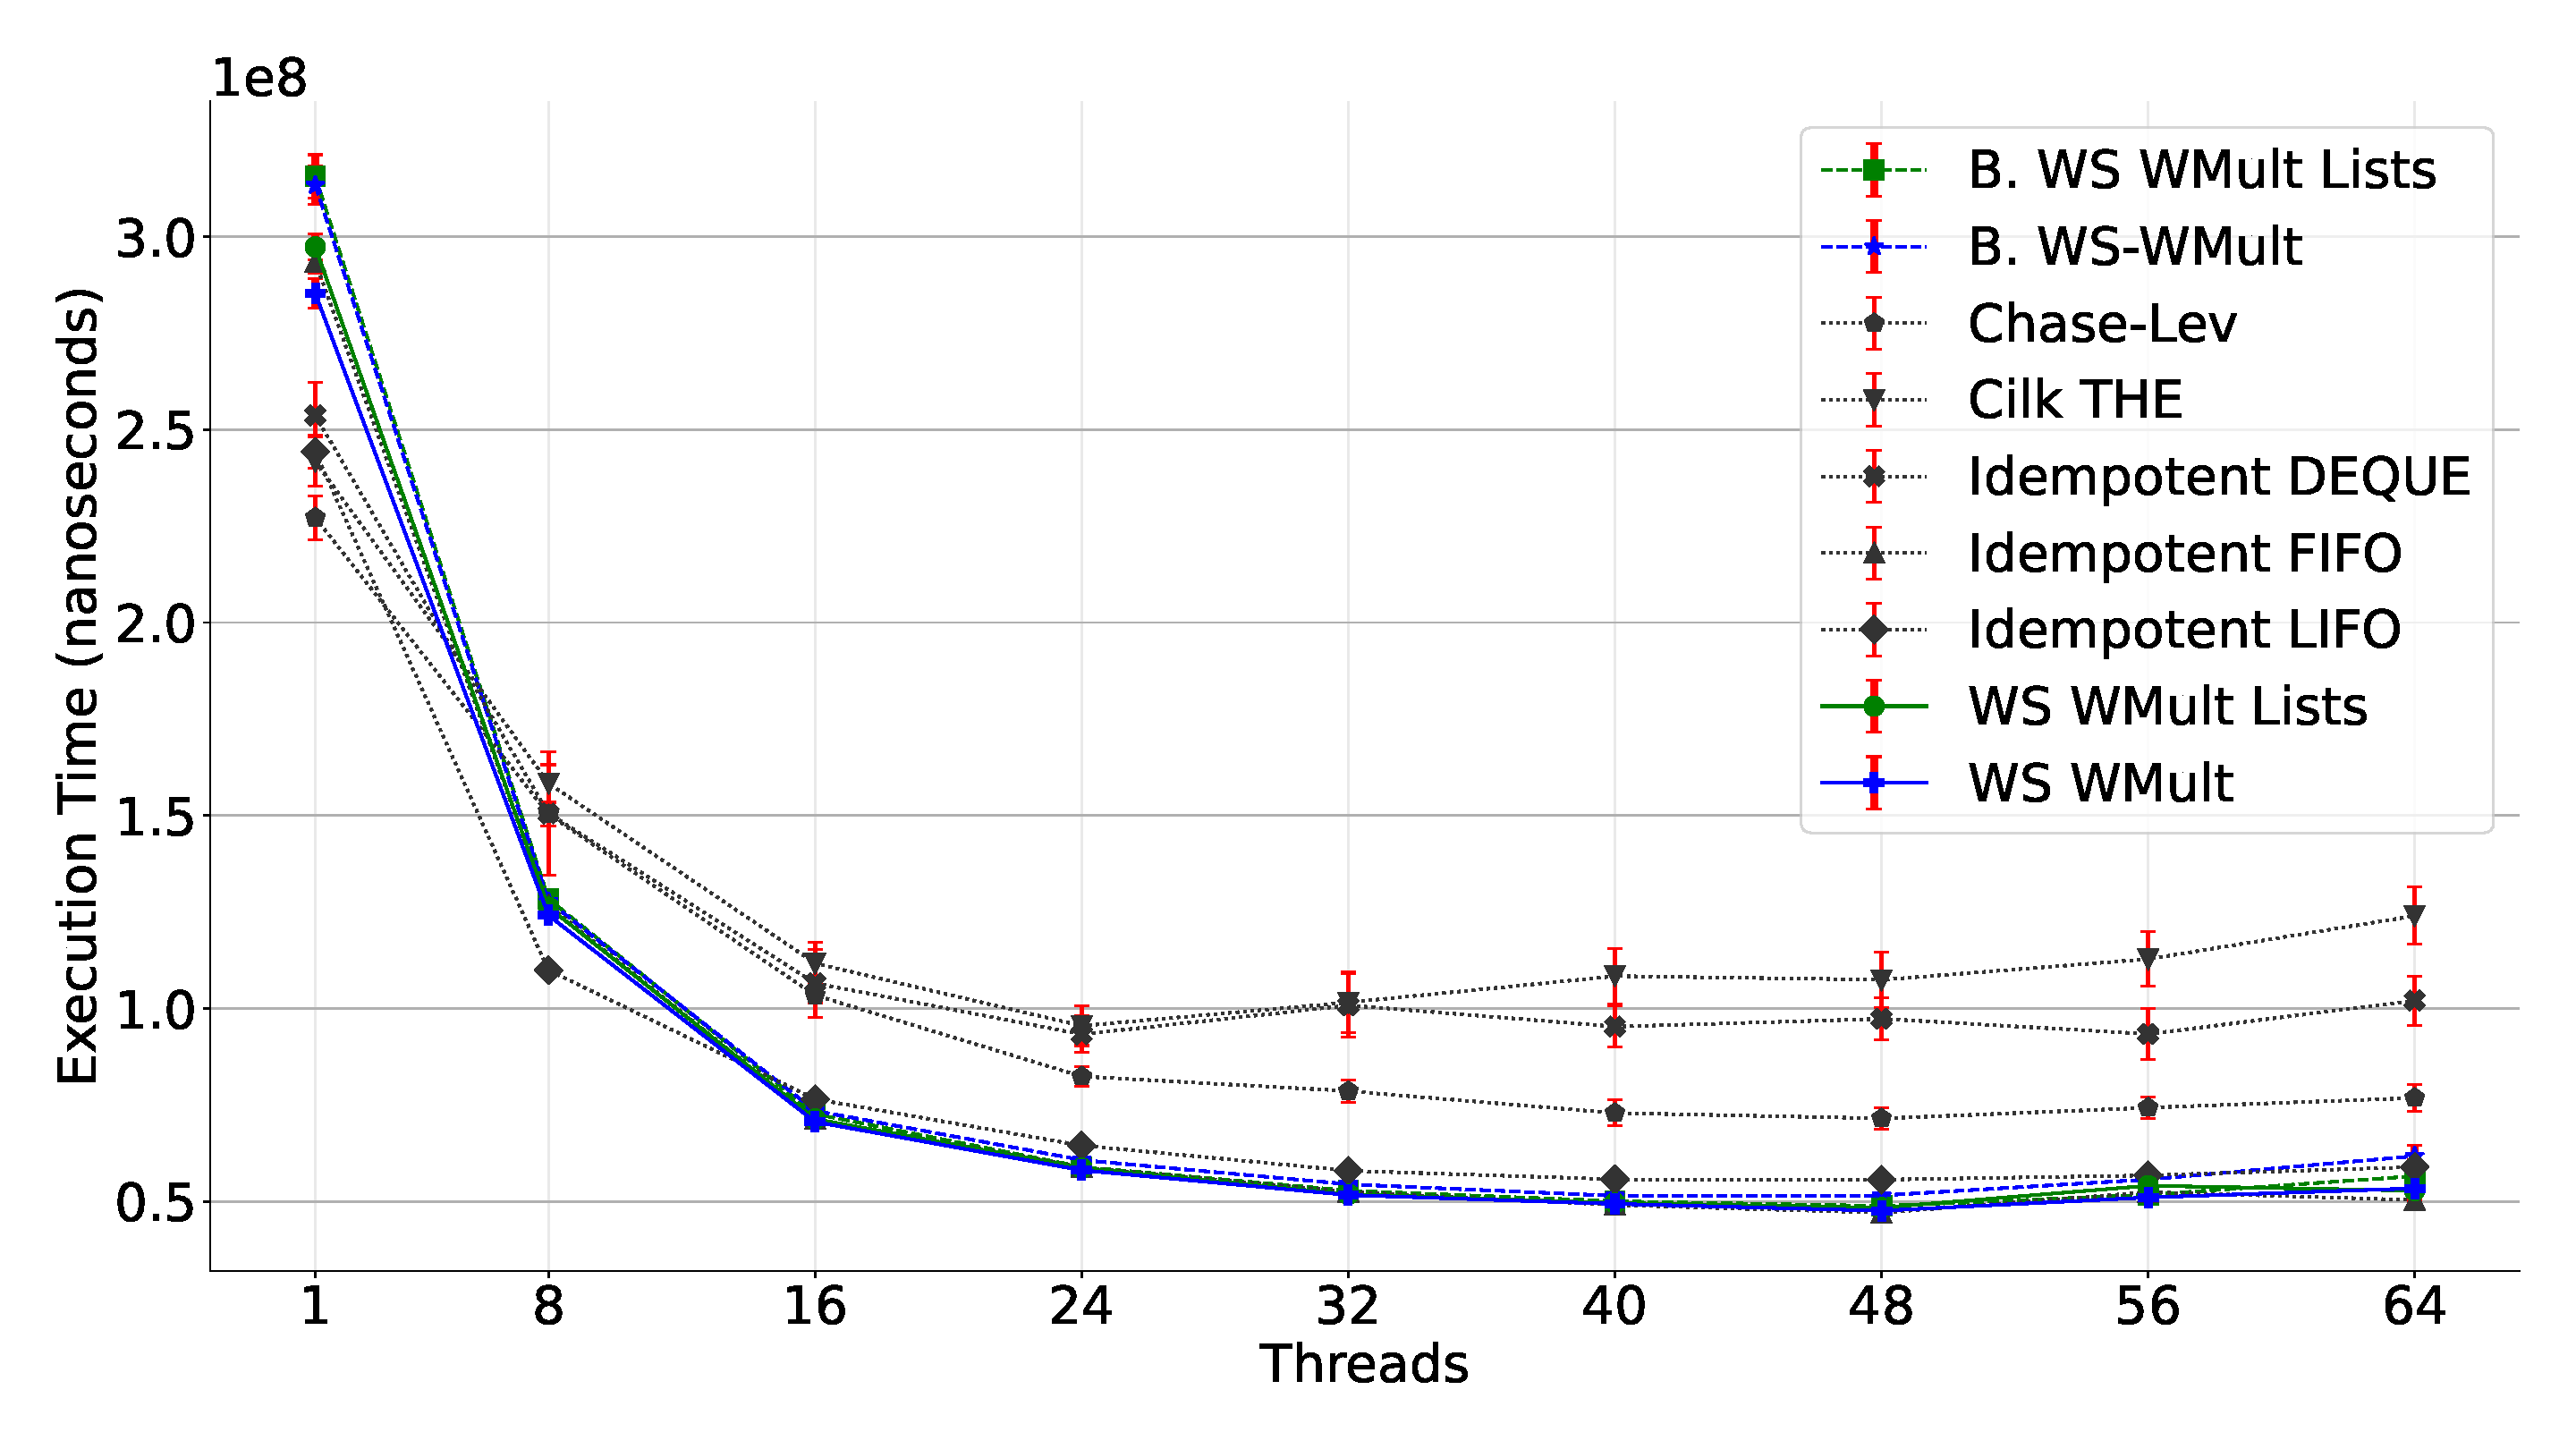
\includegraphics[width=0.48\textwidth]{contents/backmatter/evaluation/mean-TORUS2D60-Undirected-256.pdf}
  }
  \qquad
  \subfloat[\label{fig:undirected_torus2d60_1M} Mean times for the graph
  application benchmark. These are the results of the 2D Torus 60\%
  Undirected graph. For each work-stealing algorithm's
  data structure, it begins its execution with an initial size of
  1,000,000 entries.] {
    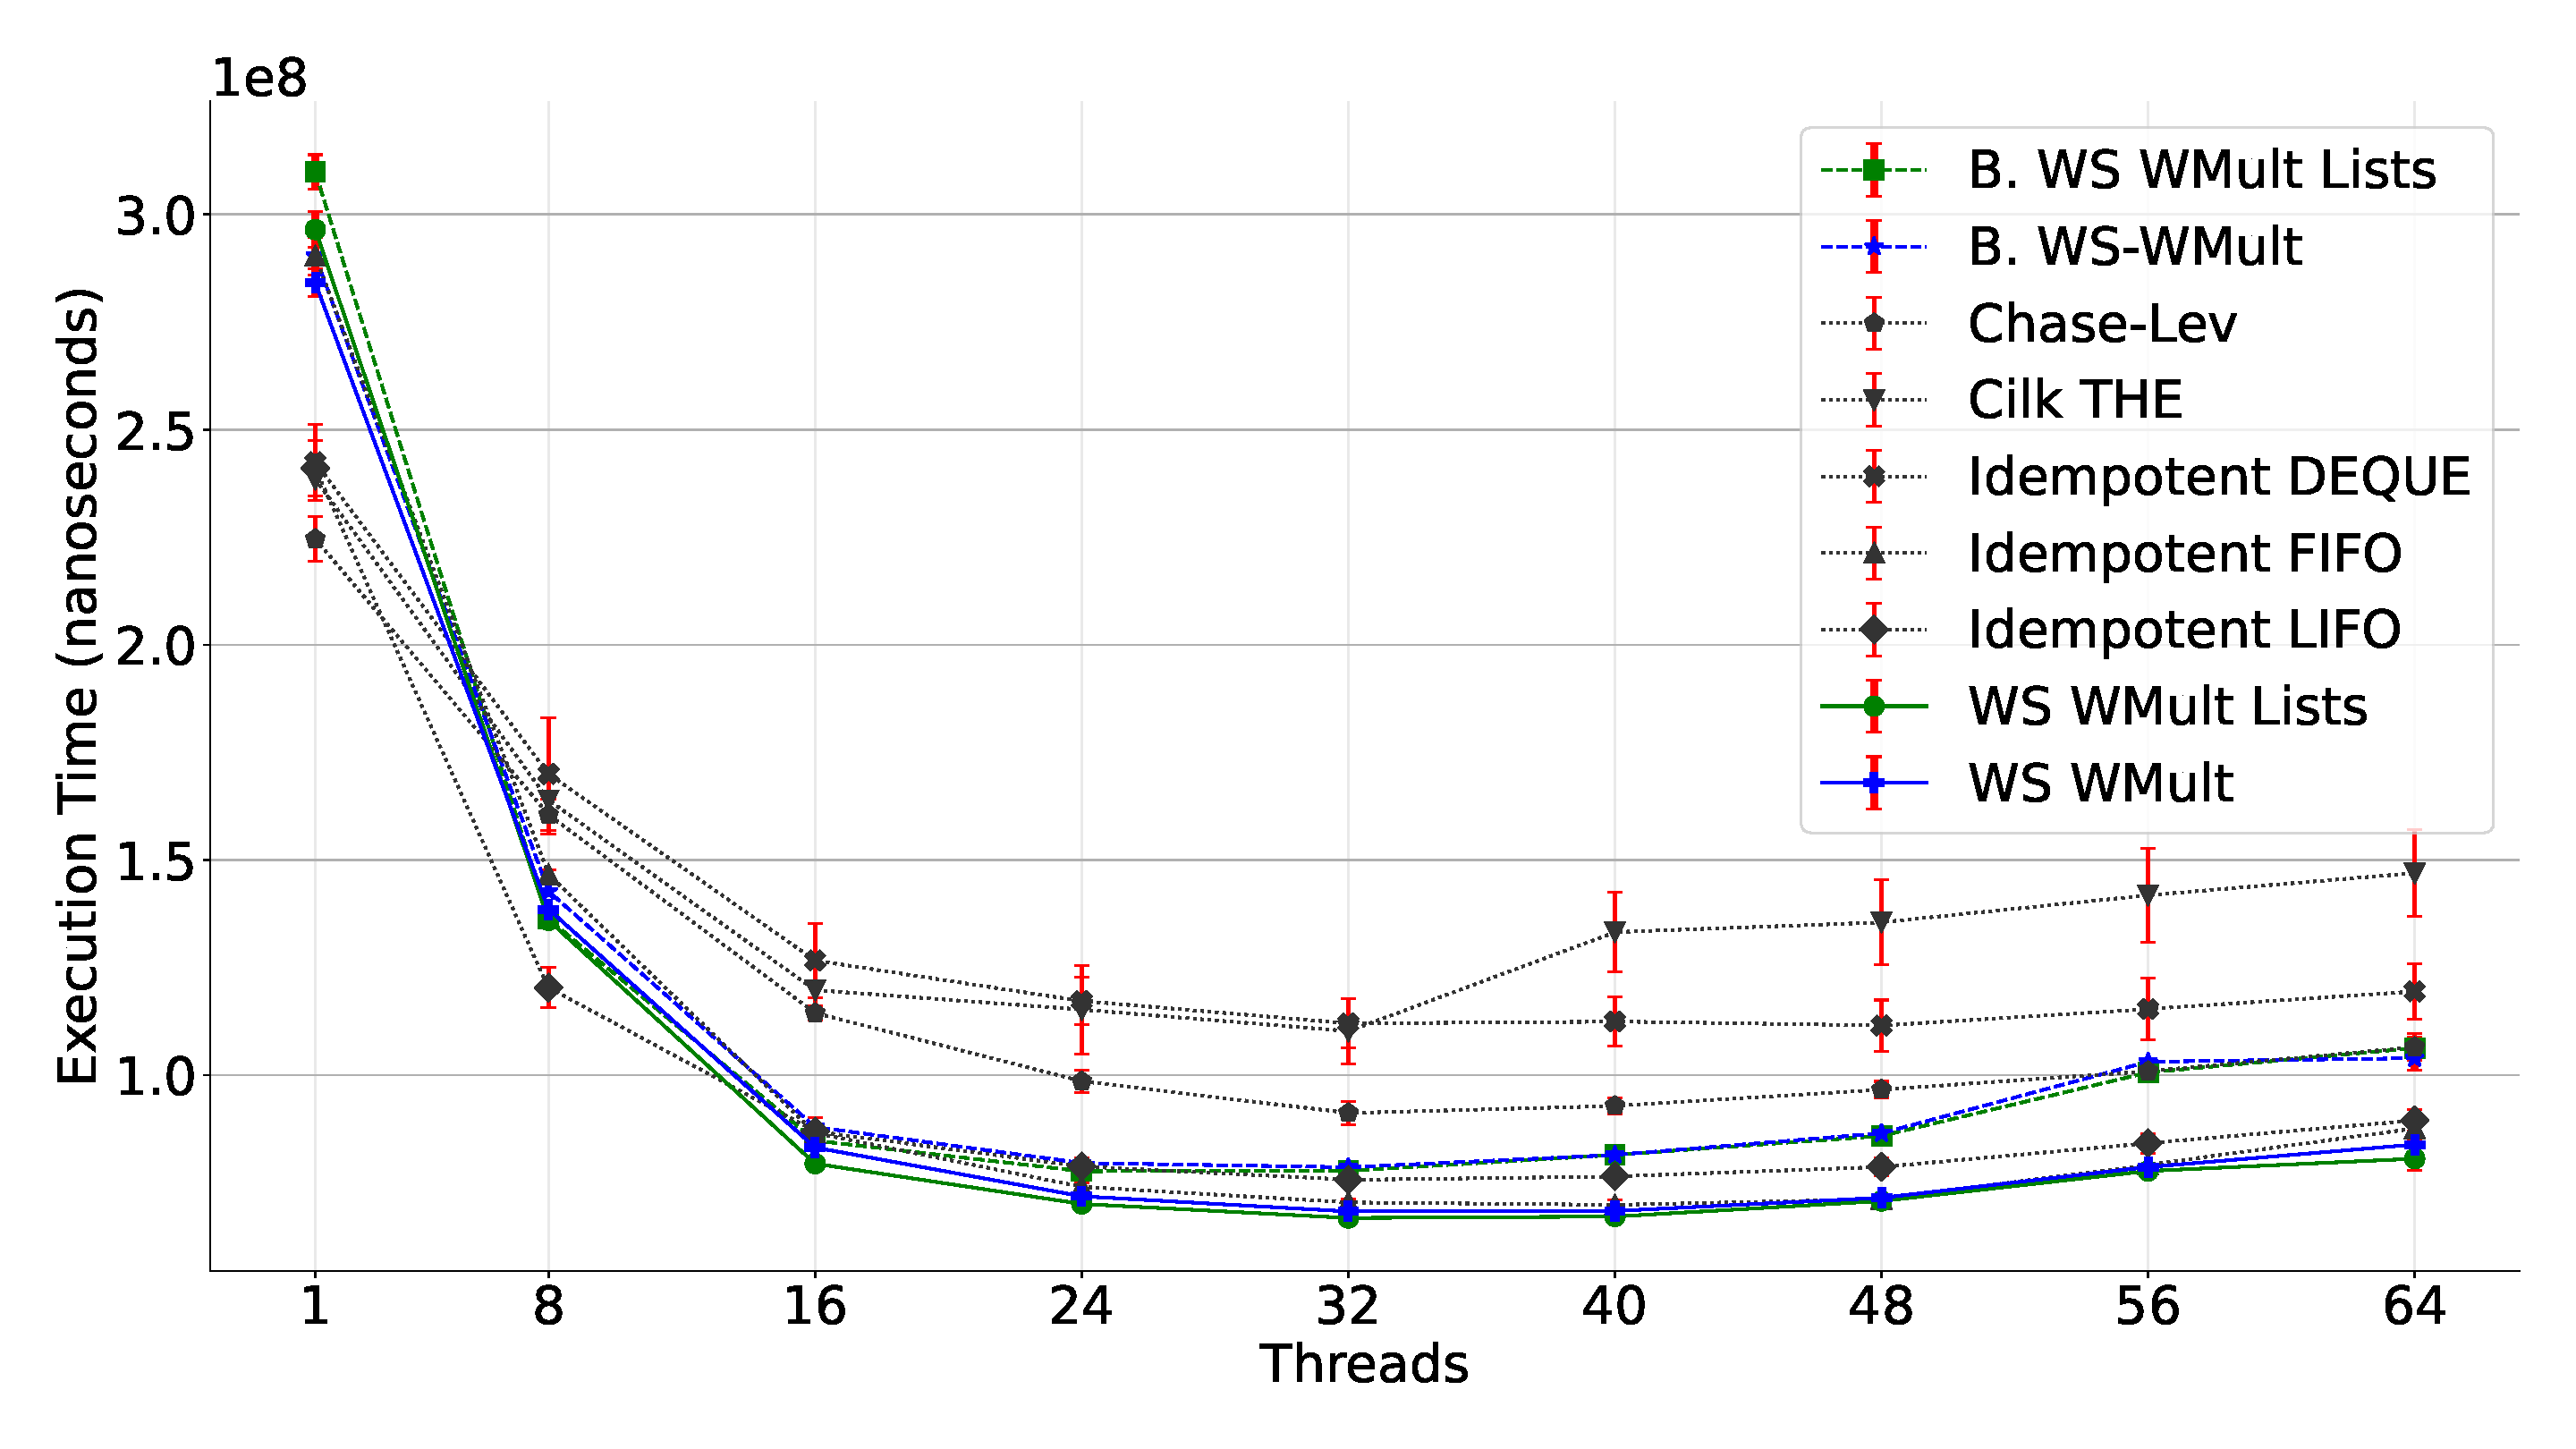
\includegraphics[width=0.48\textwidth]{contents/backmatter/evaluation/mean-TORUS2D60-Undirected-1000000.pdf}
  }
  \caption{\label{fig:2d60_torus_appendix} 2D Torus 60\% Directed and
    Undirected Graph with 256 and 1,000,000 initial sizes respectively.}
\end{figure}

\begin{table}[!ht]
\centering
\resizebox{\textwidth}{!}{\begin{tabular}{lrrrrrrrrr}
\toprule{} &           1  &           8  &          16 &          24 &          32 &          40 &          48 &          56 &          64 \\
\midrule
\textbf{B. WS WMult Lists} & 271606510.37 & 112596991.25 & 68569676.02 & 57301051.36 & 50764719.52 & 48888215.29 & 48355334.41 & 54134929.14 & 57394951.90 \\
\textbf{B. WS WMult      } & 267846777.75 & 110997123.47 & 68040897.63 & 57020102.54 & 52278828.53 & 50189180.68 & 50565768.85 & 59297832.00 & 61153079.83 \\
\textbf{Chase-Lev        } & 158506506.33 & 143484647.03 & 84147418.00 & 68976751.32 & 62140583.83 & 57845418.33 & 58101207.31 & 62954762.83 & 66131499.15 \\
\textbf{Cilk THE         } & 169847040.68 & 144015298.42 & 82866364.81 & 66790422.97 & 60273306.47 & 58391753.66 & 59823679.89 & 61730076.35 & 63568056.79 \\
\textbf{Idempotent DEQUE } & 160055984.00 & 102061319.64 & 90198138.78 & 82973638.50 & 81645834.10 & 82150883.36 & 83227444.86 & 84420556.12 & 86499396.64 \\
\textbf{Idempotent FIFO  } & 246549072.59 & 108976897.48 & 65641256.85 & 55840030.43 & 50411383.53 & 47746138.13 & 47814235.24 & 52140361.59 & 54387574.39 \\
\textbf{Idempotent LIFO  } & 176418657.30 & 136781388.73 & 79376036.88 & 65015427.06 & 58639994.94 & 54894622.52 & 54955449.08 & 59872541.30 & 63279878.32 \\
\textbf{WS WMult Lists   } & 258595656.45 & 109902199.41 & 66031946.41 & 56068001.08 & 50130919.94 & 47661233.40 & 48538151.53 & 52661930.18 & 57048192.31 \\
\textbf{WS WMult         } & 244164548.83 & 106927739.38 & 64424631.37 & 55088020.64 & 49565809.86 & 47789569.96 & 47079594.83 & 52927191.06 & 53077060.64 \\
\bottomrule
\end{tabular}}

\caption{\label{graph-TORUS2D60-Directed-256}Mean times for the graph application
    benchmark. These are the results for the 2D Torus 60\% Directed graph. Each
    algorithm begins its execution with an initial size of 256
    items.}
\end{table}

\begin{table}[!ht]
\centering
\resizebox{\textwidth}{!}{\begin{tabular}{lrrrrrrrrr}
\toprule{} &           1  &           8  &          16 &          24 &          32 &          40 &          48 &           56 &           64 \\
\midrule
\textbf{B. WS WMult Lists} & 276019680.35 & 118608819.28 & 79879863.83 & 75368321.91 & 76921962.09 & 80232098.52 & 85462153.81 & 100530174.03 & 104015378.66 \\
\textbf{B. WS WMult      } & 250827613.38 & 127704204.84 & 86842336.67 & 80203663.41 & 78982977.31 & 81987558.65 & 89238292.37 & 102066852.80 & 108750912.15 \\
\textbf{Chase-Lev        } & 159671850.22 & 147428688.35 & 91156625.45 & 79026716.82 & 75869090.23 & 75450430.54 & 77846602.34 &  87578990.75 &  96827608.33 \\
\textbf{Cilk THE         } & 170751689.40 & 145787527.82 & 87660021.64 & 76220044.95 & 71997062.28 & 74177705.44 & 79934972.24 &  83618370.09 &  88110479.39 \\
\textbf{Idempotent DEQUE } & 182658961.84 & 144968223.58 & 91149682.18 & 83740629.10 & 82285138.84 & 82047462.08 & 80435457.82 &  85897624.22 &  90689999.84 \\
\textbf{Idempotent FIFO  } & 244991185.08 & 140245626.99 & 85598340.14 & 74238515.55 & 70912264.52 & 71469675.60 & 73935154.93 &  80825298.37 &  90538667.68 \\
\textbf{Idempotent LIFO  } & 176481668.10 & 144272589.64 & 89256520.53 & 78199274.43 & 75257101.72 & 75557372.58 & 75999435.33 &  86619269.45 &  92537025.58 \\
\textbf{WS WMult Lists   } & 258286193.60 & 122279814.84 & 76291996.09 & 68133590.83 & 66153163.63 & 66865654.60 & 69070482.60 &  76900557.87 &  80688747.87 \\
\textbf{WS WMult         } & 242540777.49 & 124338868.84 & 77031753.27 & 70801264.40 & 68030449.61 & 67980027.38 & 70670605.67 &  82555005.58 &  82774264.49 \\
\bottomrule
\end{tabular}}

\caption{\label{graph-TORUS2D60-Directed-1000000}Mean times for the graph application
    benchmark. These are the results for the 2D Torus 60\% Directed graph. Each
    algorithm begins its execution with an initial size of 1000000
    items.}
\end{table}

\begin{table}[!ht]
\centering
\resizebox{\textwidth}{!}{\begin{tabular}{lrrrrrrrrr}
\toprule{} &           1  &           8  &           16 &          24 &           32 &           40 &           48 &           56 &           64 \\
\midrule
\textbf{B. WS WMult Lists} & 315547343.65 & 128360940.38 &  72648802.92 & 58927358.92 &  52792408.11 &  50039481.98 &  48804691.21 &  51732128.93 &  56555628.45 \\
\textbf{B. WS WMult      } & 313326495.26 & 127723398.79 &  73483161.75 & 60717597.04 &  54443097.02 &  51433412.83 &  51552878.37 &  55703893.17 &  61765110.29 \\
\textbf{Chase-Lev        } & 227181330.71 & 150290622.08 & 103416065.16 & 82380750.85 &  78577017.18 &  72905889.61 &  71494636.33 &  74295370.35 &  76825437.30 \\
\textbf{Cilk THE         } & 241733376.13 & 158313912.20 & 111680955.02 & 95495931.87 & 101569649.50 & 108395508.88 & 107417568.44 & 112791812.70 & 123995328.19 \\
\textbf{Idempotent DEQUE } & 253631054.34 & 150531220.36 & 106522134.60 & 93301475.32 & 100813833.08 &  95285547.84 &  97328945.64 &  93391967.26 & 102039301.48 \\
\textbf{Idempotent FIFO  } & 293454305.80 & 126736415.05 &  71307930.79 & 58829639.90 &  52462841.41 &  49072818.39 &  47060387.78 &  52425106.09 &  50348606.01 \\
\textbf{Idempotent LIFO  } & 244193909.45 & 109910536.53 &  76506588.60 & 64495660.08 &  57956406.18 &  55706367.83 &  55631734.30 &  56756671.07 &  58952951.58 \\
\textbf{WS WMult Lists   } & 297318338.24 & 126209394.42 &  71354059.76 & 58646037.82 &  51841644.46 &  49599705.40 &  48392678.56 &  54069070.60 &  52808540.08 \\
\textbf{WS WMult         } & 285278176.72 & 124107241.78 &  70627418.10 & 58085150.05 &  51669687.98 &  49369980.00 &  47603702.40 &  51037809.72 &  53382542.26 \\
\bottomrule
\end{tabular}}

\caption{\label{graph-TORUS2D60-Undirected-256}Mean times for the graph application
    benchmark. These are the results for the 2D Torus 60\% Undirected graph. Each
    algorithm begins its execution with an initial size of 256
    items.}
\end{table}

\begin{table}[!ht]
\centering
\resizebox{\textwidth}{!}{\begin{tabular}{lrrrrrrrrr}
\toprule{} &           1  &           8  &           16 &           24 &           32 &           40 &           48 &           56 &           64 \\
\midrule
\textbf{B. WS WMult Lists} & 309856315.98 & 136303438.88 &  84801109.48 &  77676595.01 &  77760793.85 &  81481981.85 &  85896394.19 & 100627631.63 & 106309709.93 \\
\textbf{B. WS WMult      } & 290354542.52 & 142736854.03 &  87950406.31 &  79587545.45 &  78588242.76 &  81475207.56 &  86517784.67 & 103123341.20 & 103949351.04 \\
\textbf{Chase-Lev        } & 224603931.97 & 160504055.83 & 114446930.51 &  98575701.24 &  91205053.43 &  92858685.79 &  96642196.09 & 100917291.75 & 106538505.87 \\
\textbf{Cilk THE         } & 238559704.41 & 163907735.92 & 119766251.42 & 115236994.47 & 110200387.50 & 133250227.29 & 135537288.52 & 141820918.53 & 146968210.28 \\
\textbf{Idempotent DEQUE } & 242414652.28 & 169993061.78 & 126641918.18 & 117239442.28 & 112027599.84 & 112470998.08 & 111536200.72 & 115373385.14 & 119482468.00 \\
\textbf{Idempotent FIFO  } & 290306090.80 & 146658908.67 &  86560565.57 &  74055672.27 &  70429908.94 &  69865238.79 &  71211933.45 &  79175134.19 &  87616728.40 \\
\textbf{Idempotent LIFO  } & 241003755.68 & 120340684.91 &  86919528.18 &  78779290.43 &  75678791.80 &  76471373.39 &  78683534.58 &  84196068.70 &  89505827.99 \\
\textbf{WS WMult Lists   } & 296513168.96 & 135982366.57 &  79425785.45 &  70076106.00 &  66821235.21 &  67149530.26 &  70754231.29 &  77729508.08 &  80592631.25 \\
\textbf{WS WMult         } & 284133861.51 & 138538767.64 &  83190684.63 &  71858766.90 &  68338658.79 &  68446034.77 &  71509952.60 &  78648218.58 &  83889876.34 \\
\bottomrule
\end{tabular}}

\caption{\label{graph-TORUS2D60-Undirected-1000000}Mean times for the graph application
    benchmark. These are the results for the 2D Torus 60\% Undirected graph. Each
    algorithm begins its execution with an initial size of 1000000
    items.}
\end{table}


\begin{figure}[!ht]
  \subfloat[\label{fig:directed_torus3d_256} Mean times for the graph
  application benchmark. These are the results of the 3D Torus
  Directed graph. For each work-stealing algorithm's
  data structure, it begins its execution with an initial size of
  256 entries.] {
    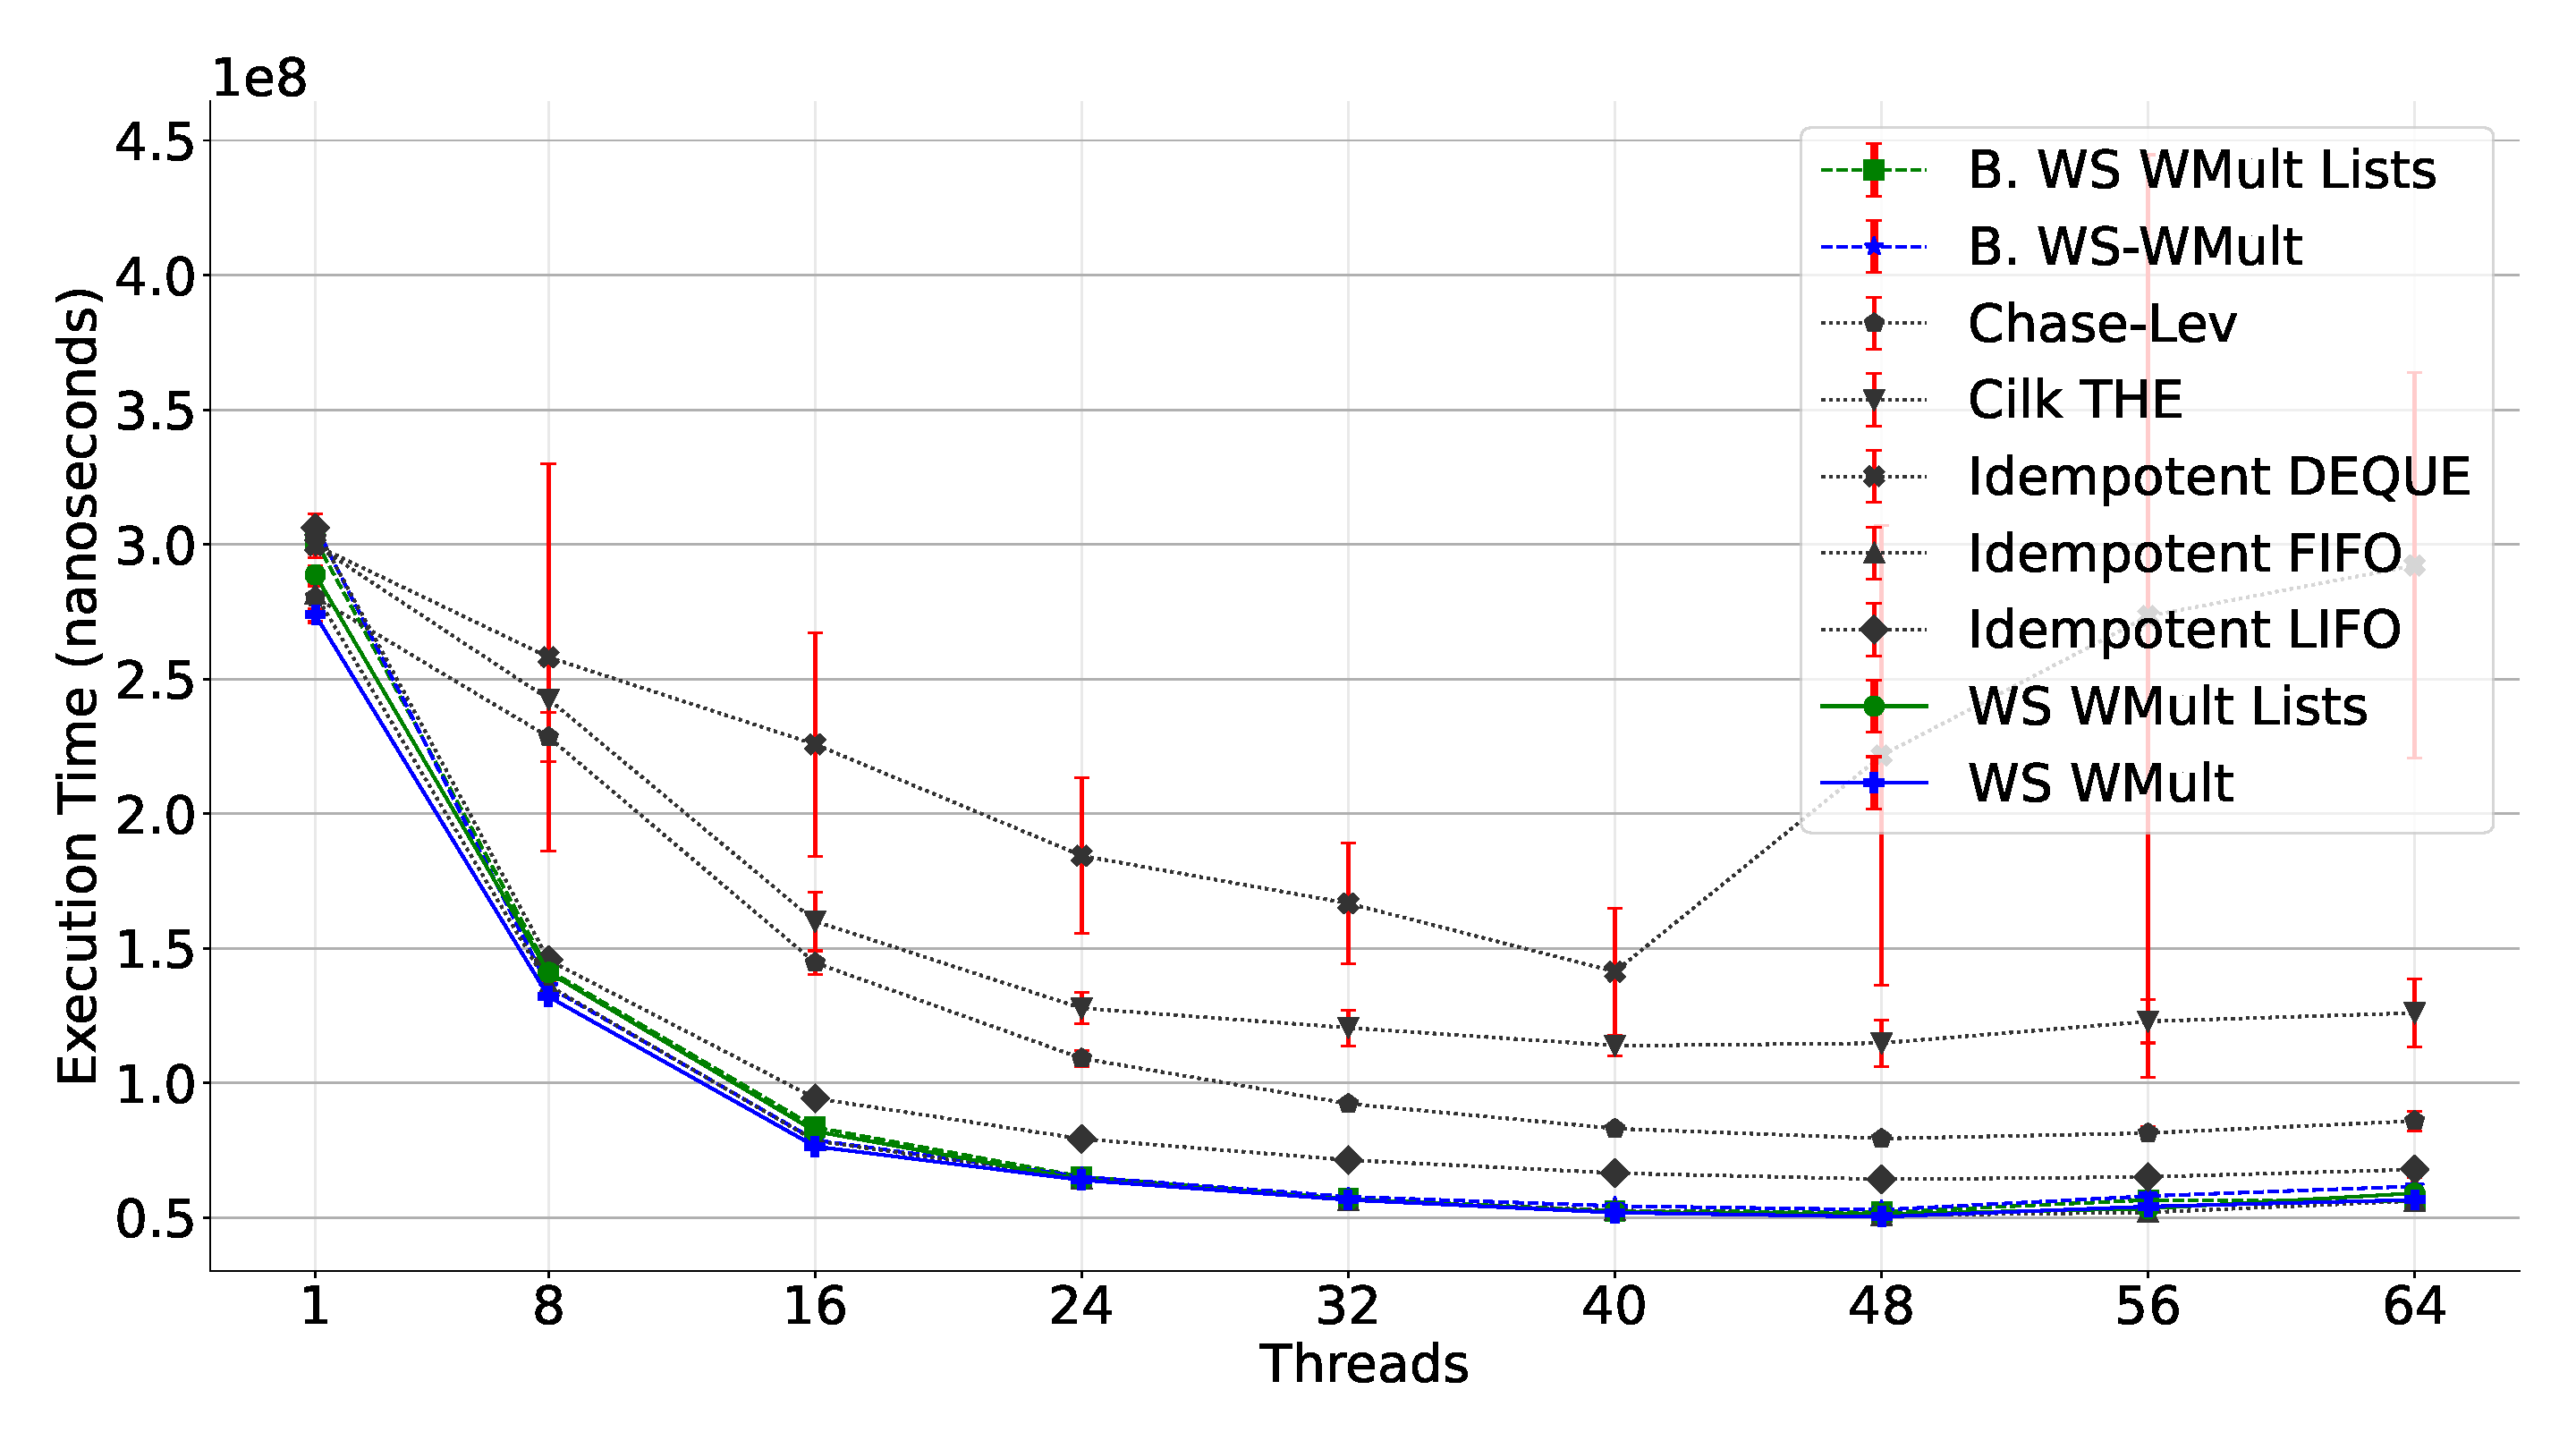
\includegraphics[width=0.48\textwidth]{contents/backmatter/evaluation/mean-TORUS3D-Directed-256.pdf}
  }
  \qquad
  \subfloat[\label{fig:directed_torus3d_1M} Mean times for the graph
  application benchmark. These are the results of the 3D Torus
  Directed graph. For each work-stealing algorithm's
  data structure, it begins its execution with an initial size of
  1,000,00 entries.] {
    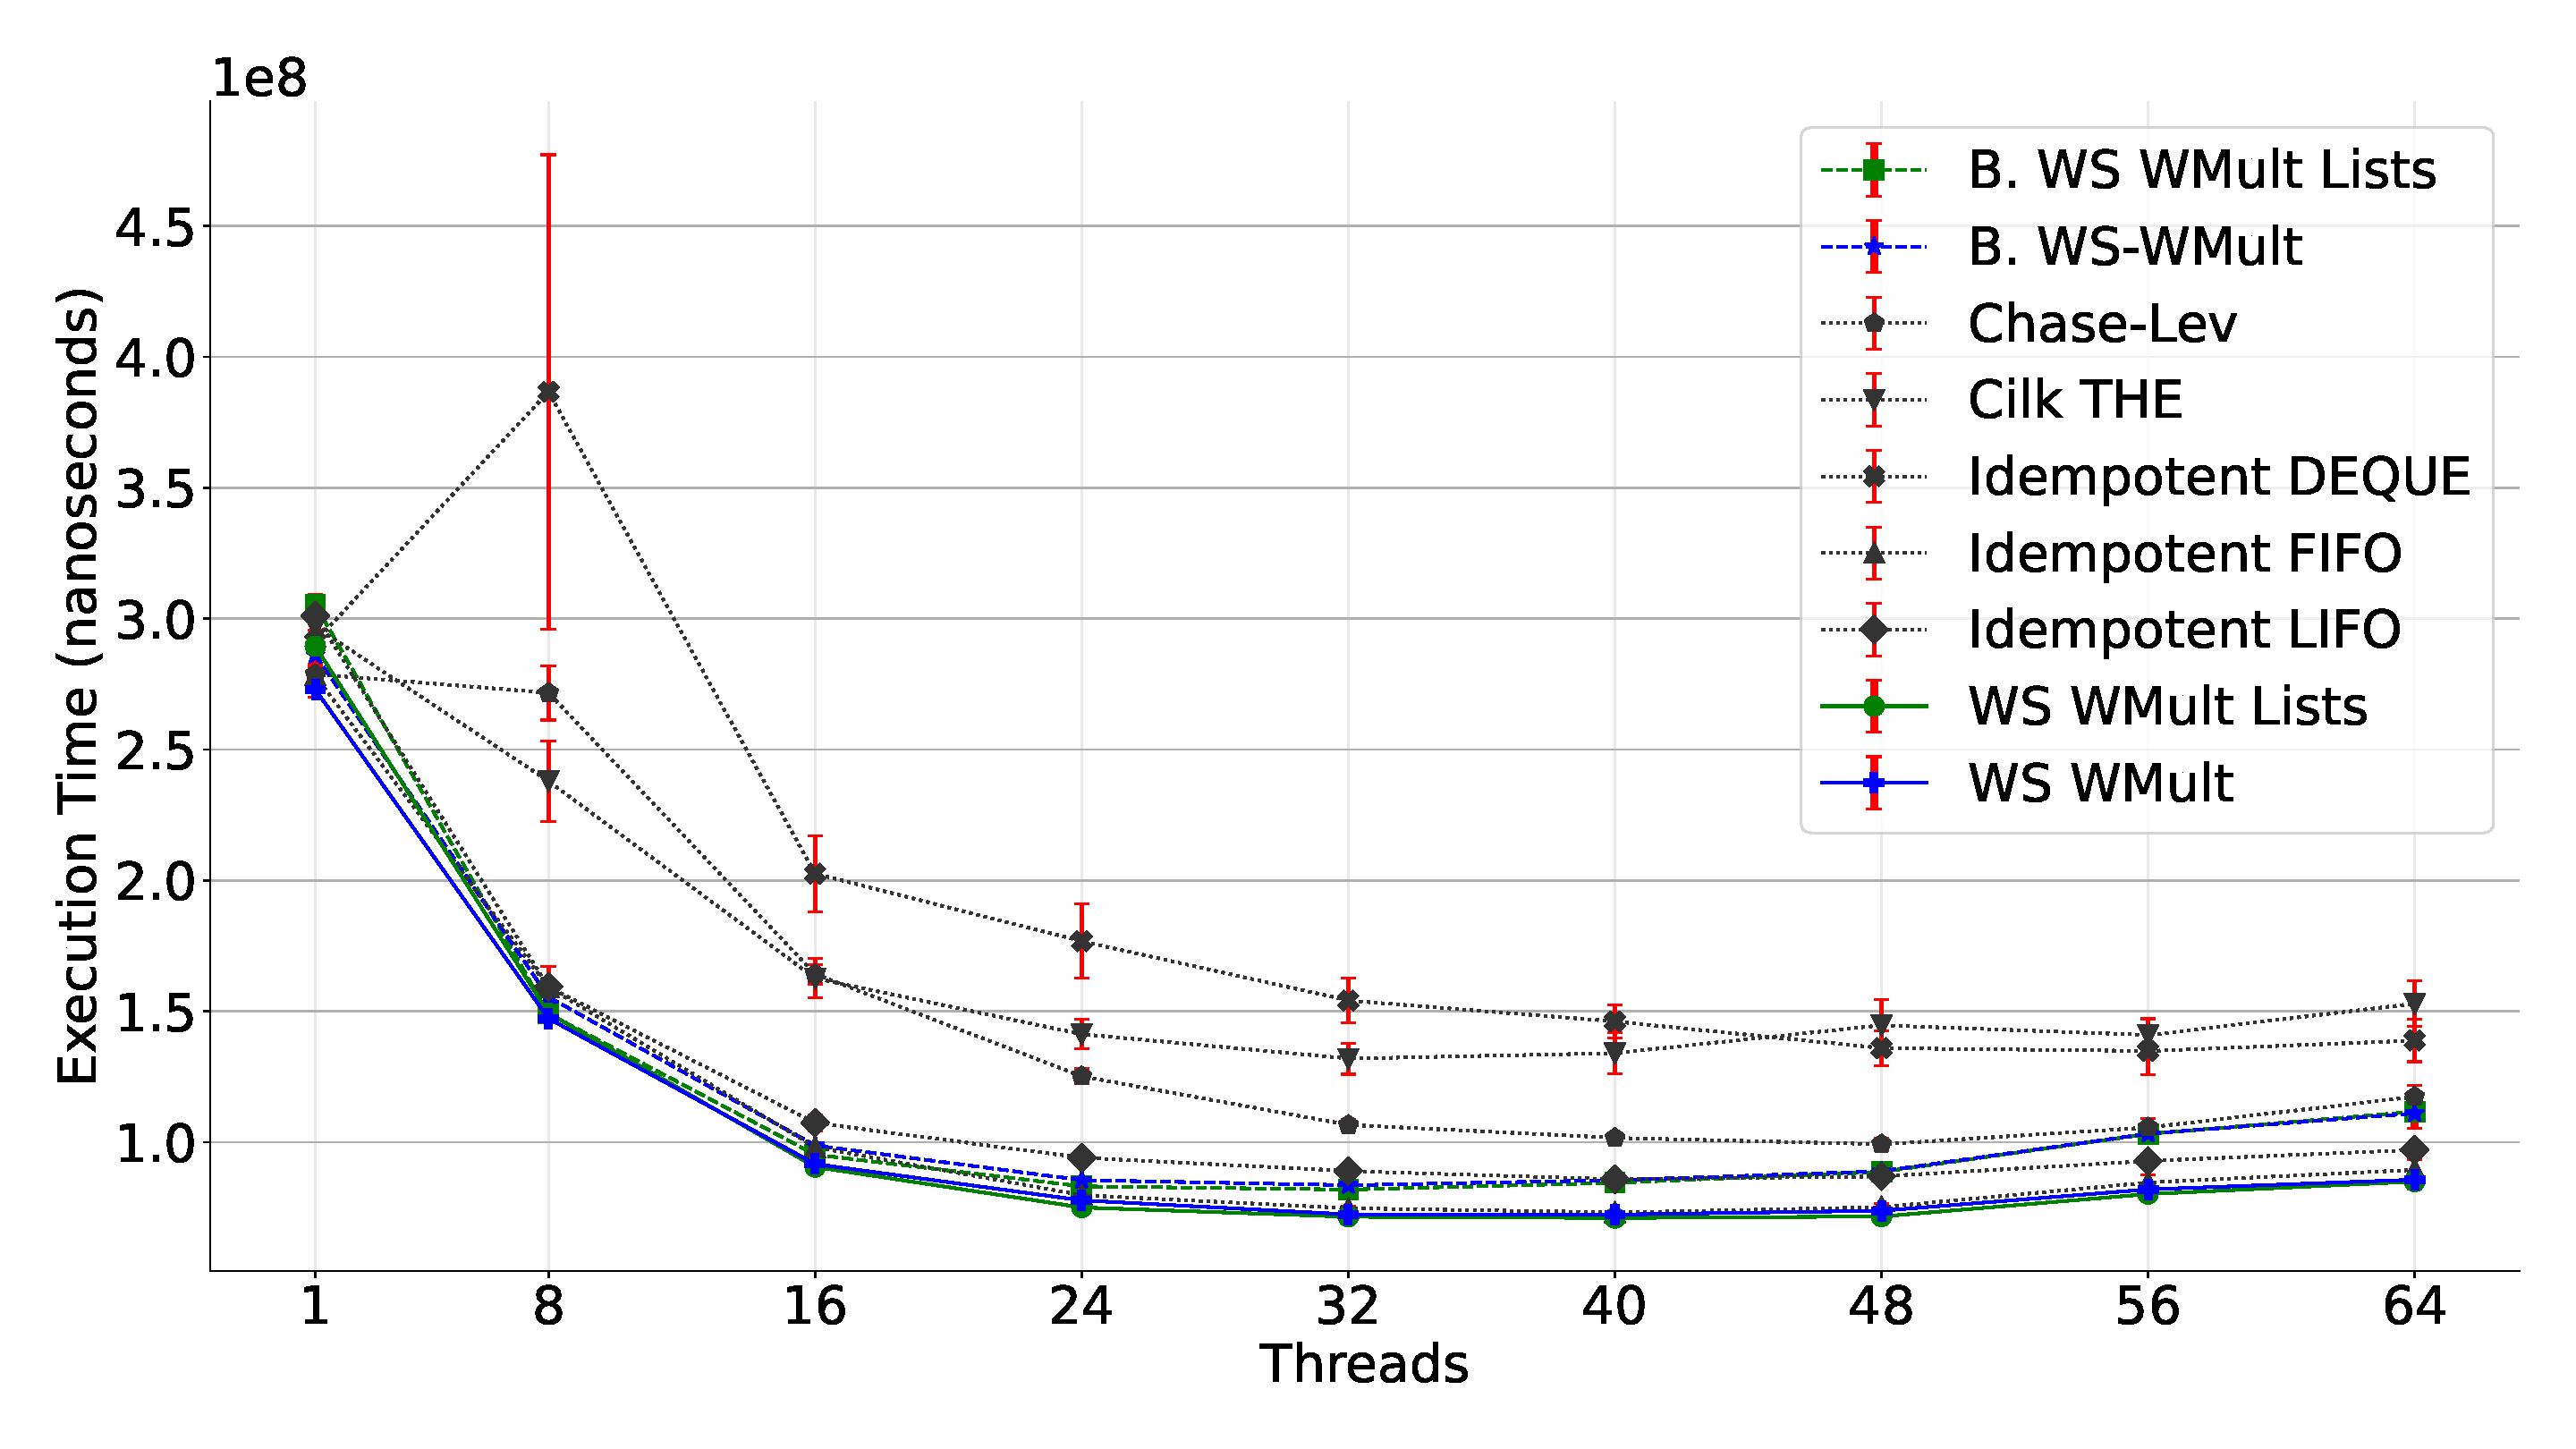
\includegraphics[width=0.48\textwidth]{contents/backmatter/evaluation/mean-TORUS3D-Directed-1000000.pdf}
  }

  \subfloat[\label{fig:undirected_torus3d_256} Mean times for the graph
  application benchmark. These are the results of the 3D Torus
  Undirected graph. For each work-stealing algorithm's
  data structure, it begins its execution with an initial size of
  256 entries.] {
    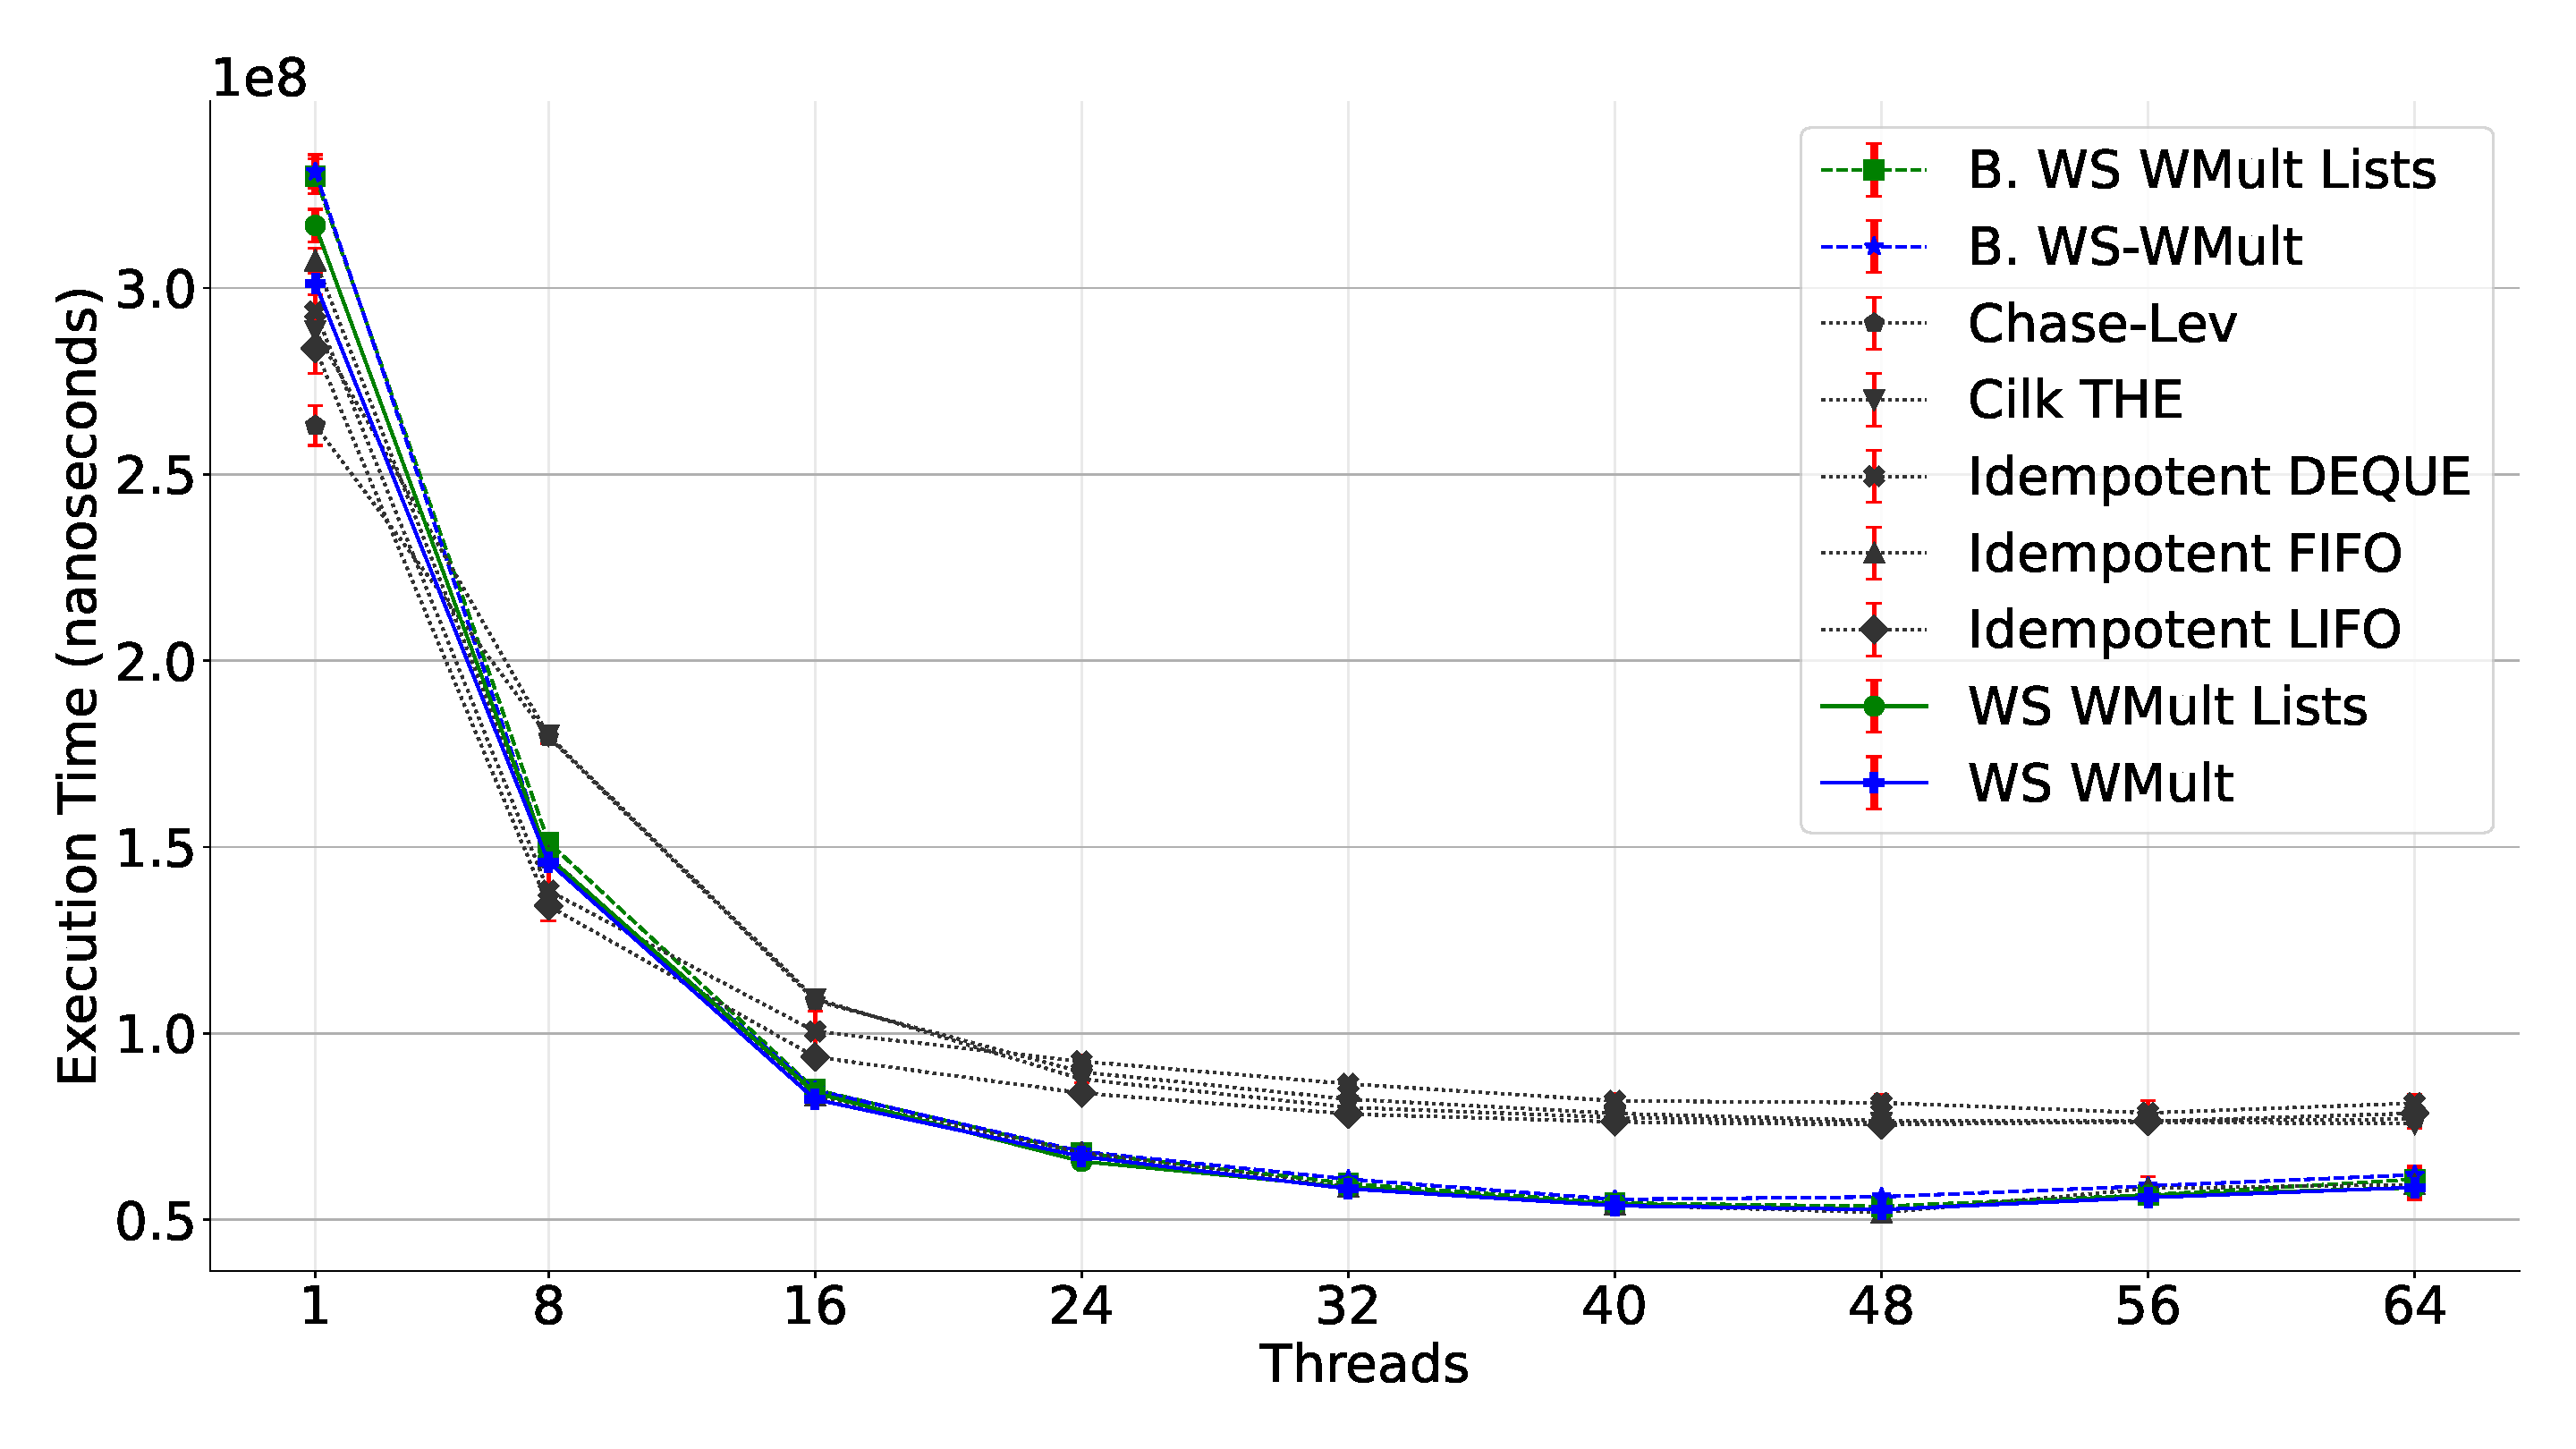
\includegraphics[width=0.48\textwidth]{contents/backmatter/evaluation/mean-TORUS3D-Undirected-256.pdf}
  }
  \qquad
  \subfloat[\label{fig:undirected_torus3d_1M} Mean times for the graph
  application benchmark. These are the results of the 3D Torus
  Undirected graph. For each work-stealing algorithm's
  data structure, it begins its execution with an initial size of
  1,000,000 entries.] {
    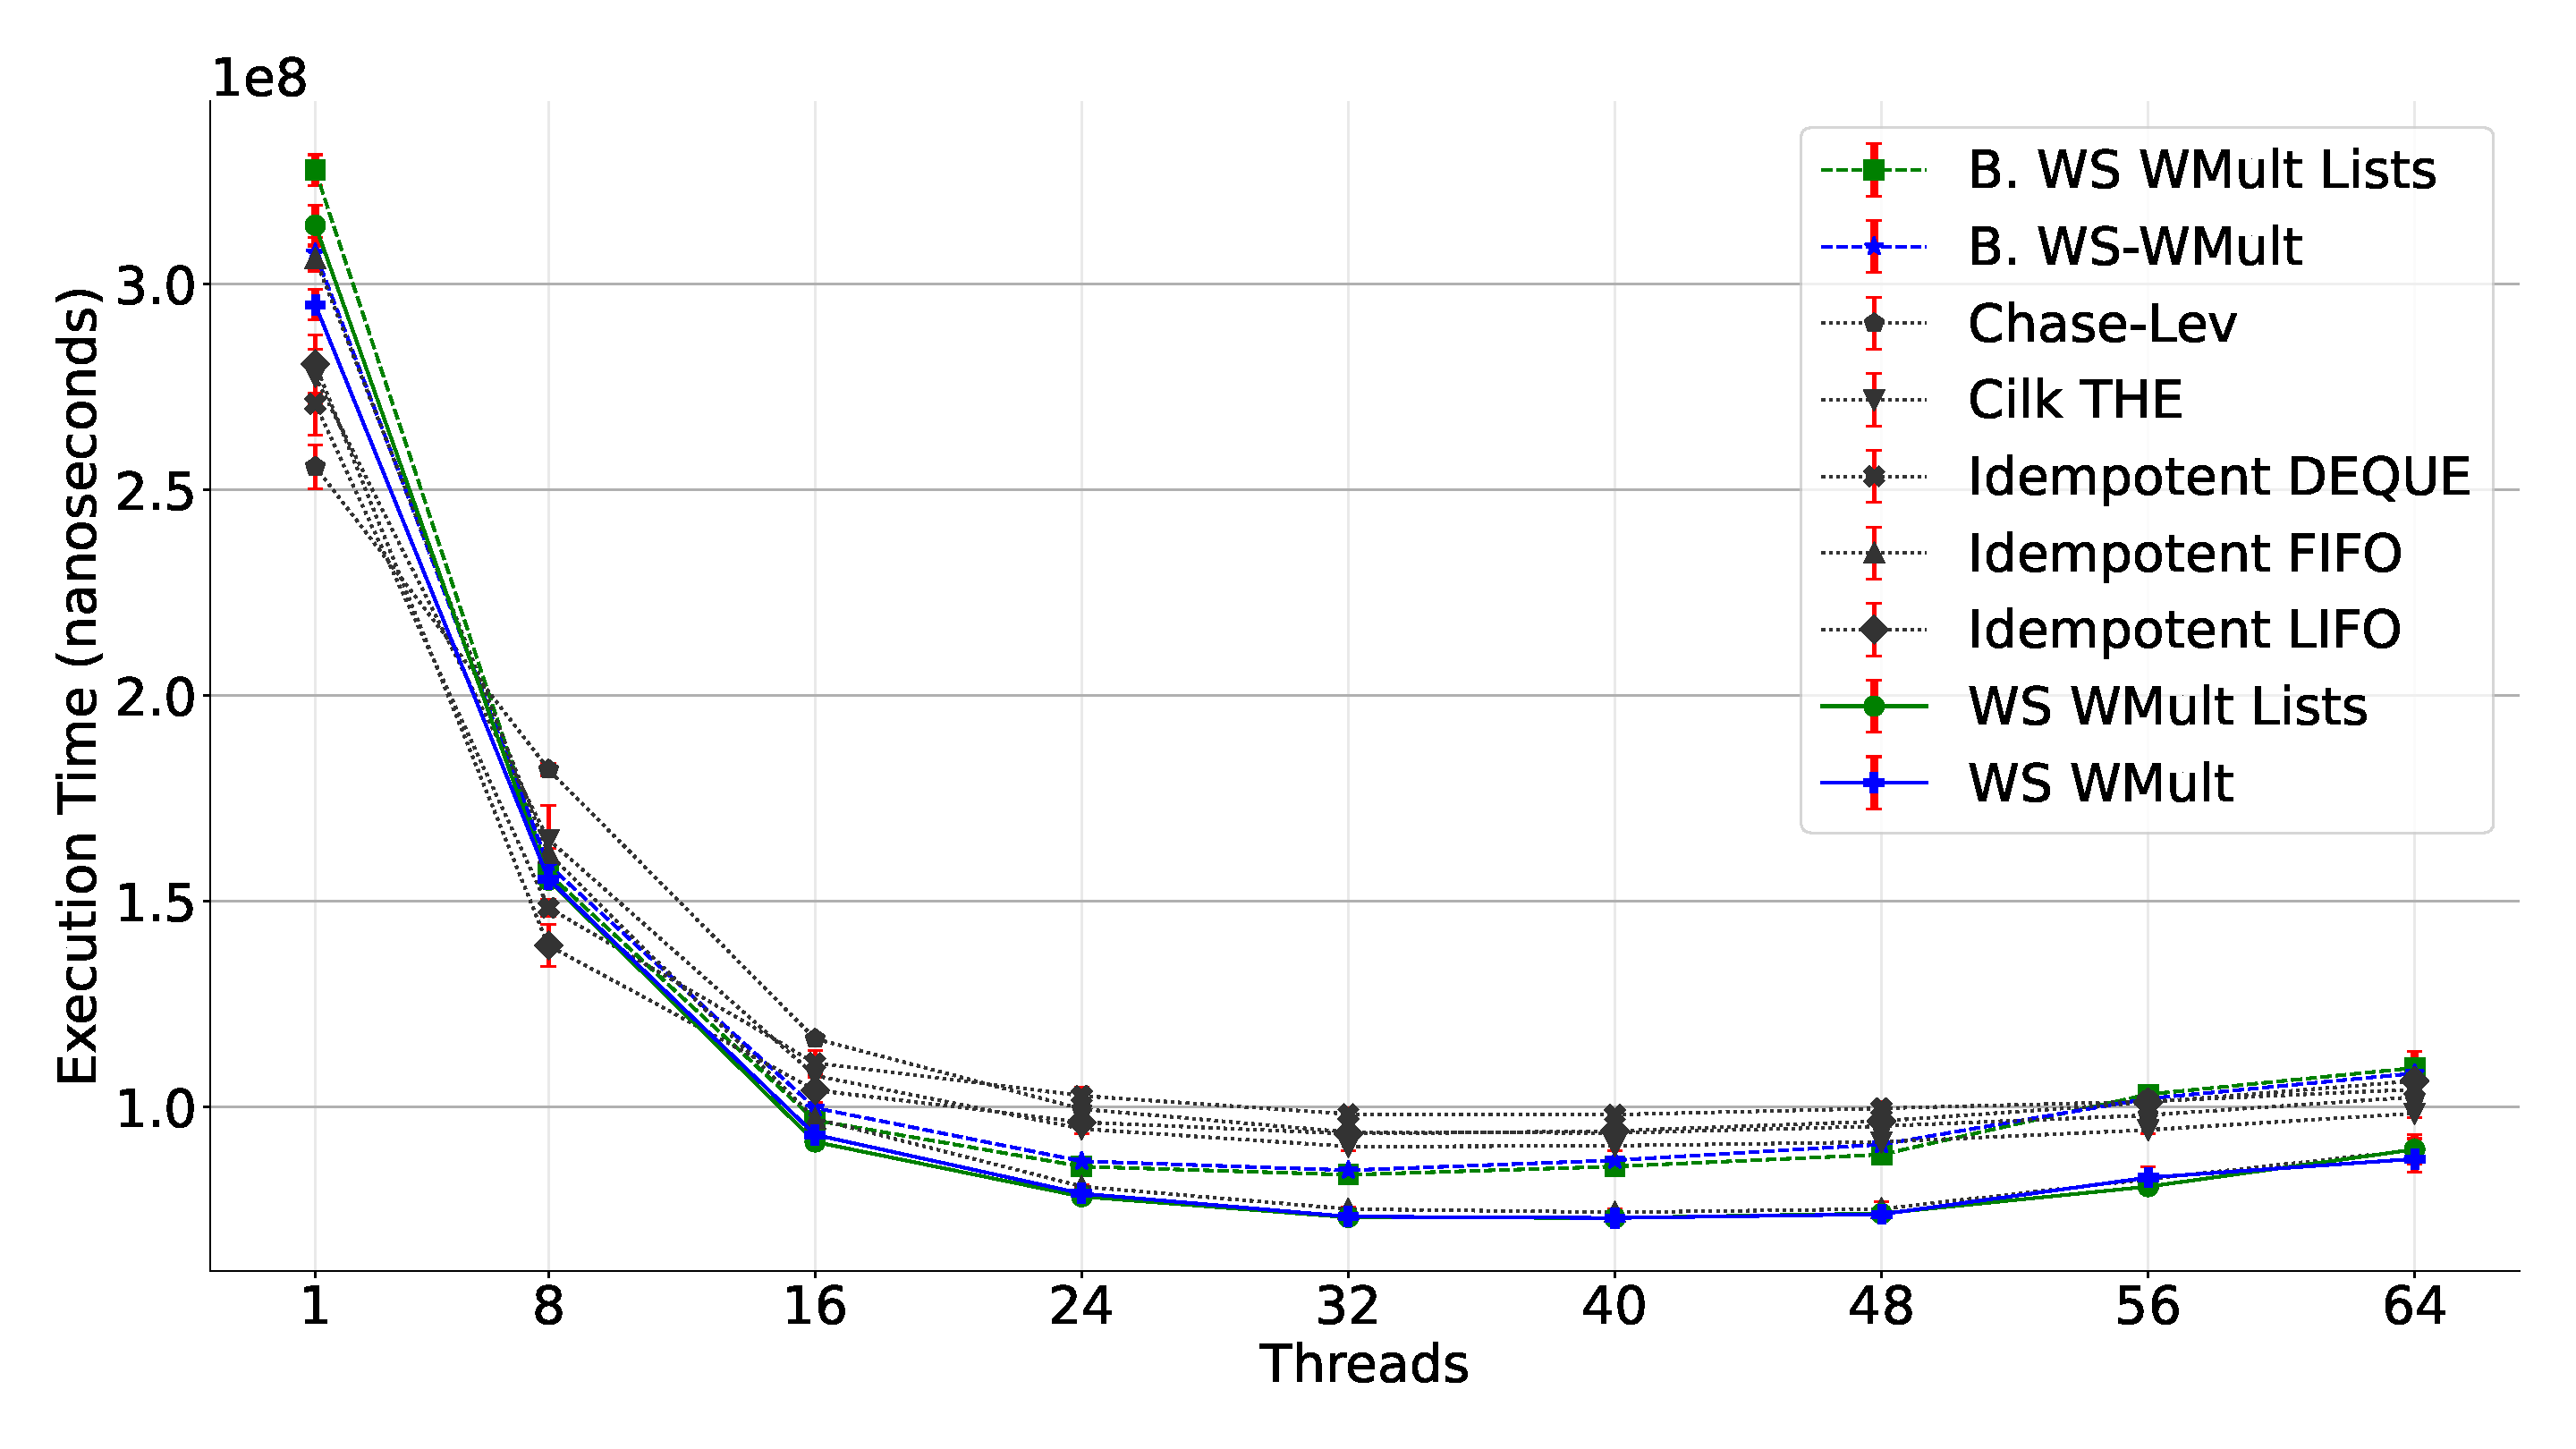
\includegraphics[width=0.48\textwidth]{contents/backmatter/evaluation/mean-TORUS3D-Undirected-1000000.pdf}
  }
  \caption{\label{fig:3d_torus_appendix} 3D Torus Directed and
    Undirected Graph with 256 and 1,000,000 initial sizes respectively.}
\end{figure}

\begin{table}[!ht]
\centering
\resizebox{\textwidth}{!}{\begin{tabular}{lrrrrrrrrr}
\toprule{} &           1  &           8  &           16 &           24 &           32 &           40 &           48 &           56 &           64 \\
\midrule
\textbf{B. WS WMult Lists} & 301624917.75 & 141866549.86 &  83541479.95 &  65138808.25 &  56914186.43 &  52423454.12 &  51989751.02 &  56527527.81 &  56014742.33 \\
\textbf{B. WS WMult      } & 307030538.52 & 135703652.72 &  78782482.95 &  65127326.79 &  57715887.45 &  54287146.47 &  52865866.01 &  57975637.71 &  61597515.65 \\
\textbf{Chase-Lev        } & 280392485.15 & 228490657.84 & 144625861.02 & 109098309.70 &  92276276.37 &  83024023.87 &  79330745.40 &  81379045.57 &  85906640.40 \\
\textbf{Cilk THE         } & 299818699.91 & 242544084.79 & 160037649.11 & 127730079.75 & 120478873.41 & 113797574.00 & 114802833.54 & 122864155.78 & 126030085.89 \\
\textbf{Idempotent DEQUE } & 299736006.28 & 258097839.40 & 225742191.98 & 184364046.70 & 166686299.08 & 141299789.18 & 221591062.68 & 273390848.52 & 292214859.04 \\
\textbf{Idempotent FIFO  } & 281603607.82 & 136152638.28 &  78509517.98 &  64302364.58 &  56427898.85 &  52667607.33 &  50843691.96 &  51910053.16 &  56209351.97 \\
\textbf{Idempotent LIFO  } & 306122801.62 & 145650799.53 &  94241295.91 &  79193284.39 &  71350221.69 &  66482956.94 &  64179470.43 &  65091183.51 &  67905411.43 \\
\textbf{WS WMult Lists   } & 288758130.76 & 141026789.51 &  82019900.84 &  64081744.46 &  56705351.91 &  52060495.93 &  51302462.90 &  53337902.56 &  59025199.96 \\
\textbf{WS WMult         } & 273827102.97 & 132030977.87 &  76413364.21 &  63917969.81 &  56562794.21 &  51825154.68 &  50271924.64 &  54089613.78 &  56571351.07 \\
\bottomrule
\end{tabular}}

\caption{\label{graph-TORUS3D-Directed-256}Mean times for the graph application
    benchmark. These are the results for the 3D Torus Directed graph. Each
    algorithm begins its execution with an initial size of 256
    items.}
\end{table}

\begin{table}[!ht]
\centering
\resizebox{\textwidth}{!}{\begin{tabular}{lrrrrrrrrr}
\toprule{} &           1  &           8  &           16 &           24 &           32 &           40 &           48 &           56 &           64 \\
\midrule
\textbf{B. WS WMult Lists} & 305386171.91 & 149046365.13 &  95194976.05 &  83089189.21 &  81849733.73 &  84456797.58 &  88612485.27 & 103127683.01 & 111643788.60 \\
\textbf{B. WS WMult      } & 286170202.17 & 155416147.14 &  98692484.33 &  85463352.85 &  83512427.37 &  85456104.05 &  88874130.18 & 103205452.01 & 111004273.95 \\
\textbf{Chase-Lev        } & 278736420.94 & 271617495.59 & 164154925.33 & 125110061.65 & 106566596.33 & 101604051.41 &  99166808.03 & 105596223.23 & 117346843.22 \\
\textbf{Cilk THE         } & 296880199.62 & 237861235.97 & 162585819.44 & 141211156.01 & 131884833.85 & 133994568.66 & 144624731.92 & 140846305.32 & 152922059.48 \\
\textbf{Idempotent DEQUE } & 291164788.92 & 386607331.02 & 202531346.52 & 176731787.64 & 154063302.46 & 146056409.62 & 135880453.30 & 134783560.36 & 138854522.50 \\
\textbf{Idempotent FIFO  } & 278180866.51 & 159103860.27 &  98048277.27 &  79703731.70 &  74716915.26 &  73100122.13 &  75161749.36 &  84572371.02 &  89422809.81 \\
\textbf{Idempotent LIFO  } & 301046988.65 & 159255115.41 & 107324698.34 &  94007081.70 &  88918399.30 &  85772169.76 &  86925836.93 &  92797785.35 &  97037925.58 \\
\textbf{WS WMult Lists   } & 289429455.36 & 149254306.51 &  90492036.98 &  75025116.54 &  71479061.67 &  71015053.44 &  71581342.57 &  80150110.38 &  84911758.39 \\
\textbf{WS WMult         } & 272901359.61 & 147192902.24 &  91605903.29 &  77732968.05 &  72367652.95 &  72288630.73 &  73772772.47 &  81914543.31 &  85625911.00 \\
\bottomrule
\end{tabular}}

\caption{\label{graph-TORUS3D-Directed-1000000}Mean times for the graph application
    benchmark. These are the results for the 3D Torus Directed graph. Each
    algorithm begins its execution with an initial size of 1000000
    items.}
\end{table}

\begin{table}[!ht]
\centering
\resizebox{\textwidth}{!}{\begin{tabular}{lrrrrrrrrr}
\toprule{} &           1  &           8  &           16 &          24 &          32 &          40 &          48 &          56 &          64 \\
\midrule
\textbf{B. WS WMult Lists} & 329963181.86 & 151237154.92 &  84869838.17 & 67958542.51 & 59713831.95 & 54468184.21 & 53567371.26 & 56654627.98 & 60827191.22 \\
\textbf{B. WS WMult      } & 331185252.48 & 146485279.46 &  84701527.73 & 68272626.35 & 60861442.11 & 55445870.97 & 56134319.33 & 59038658.18 & 62044348.75 \\
\textbf{Chase-Lev        } & 263083757.40 & 179485868.93 & 108749102.80 & 89621581.64 & 82340911.59 & 78506473.93 & 76517833.65 & 76532206.85 & 76983181.99 \\
\textbf{Cilk THE         } & 288413877.71 & 179880361.54 & 109264333.28 & 87696126.26 & 80130481.87 & 77436833.45 & 75972286.49 & 76154694.41 & 75715301.52 \\
\textbf{Idempotent DEQUE } & 293601547.68 & 138258919.26 & 100495723.16 & 92474474.20 & 86429098.06 & 81863930.54 & 81369974.02 & 78652635.16 & 81262219.14 \\
\textbf{Idempotent FIFO  } & 307245700.44 & 147417337.93 &  83189889.36 & 67974190.23 & 58801237.69 & 53994442.80 & 51875146.32 & 58401317.40 & 59453077.65 \\
\textbf{Idempotent LIFO  } & 283722458.29 & 134208645.80 &  93649945.13 & 83971242.41 & 78331924.14 & 76256331.63 & 75417609.21 & 76412158.70 & 78572650.04 \\
\textbf{WS WMult Lists   } & 316728772.49 & 147223826.60 &  83985379.30 & 65631752.33 & 58718689.24 & 54261373.97 & 52678773.73 & 56547641.85 & 58570046.69 \\
\textbf{WS WMult         } & 301154107.56 & 145915148.41 &  82284655.05 & 66963616.84 & 58307819.83 & 53742415.50 & 52712760.46 & 55935847.51 & 58660468.71 \\
\bottomrule
\end{tabular}}

\caption{\label{graph-TORUS3D-Undirected-256}Mean times for the graph application
    benchmark. These are the results for the 3D Torus Undirected graph. Each
    algorithm begins its execution with an initial size of 256
    items.}
\end{table}

\begin{table}[!ht]
\centering
\resizebox{\textwidth}{!}{\begin{tabular}{lrrrrrrrrr}
\toprule{} &           1  &           8  &           16 &           24 &          32 &          40 &          48 &           56 &           64 \\
\midrule
\textbf{B. WS WMult Lists} & 327707616.44 & 156712246.64 &  96753448.36 &  85516751.68 & 83516731.27 & 85541958.28 & 88430855.09 & 103074767.38 & 109510162.32 \\
\textbf{B. WS WMult      } & 307644871.81 & 158759098.92 &  99763923.60 &  86807733.13 & 84602962.87 & 87048309.48 & 90879164.43 & 102032203.69 & 108190237.33 \\
\textbf{Chase-Lev        } & 255662963.74 & 182008226.94 & 116576204.10 &  99491054.93 & 93867107.54 & 93663588.23 & 95350740.85 &  98024792.96 & 102423692.66 \\
\textbf{Cilk THE         } & 277586748.65 & 164994070.46 & 107628297.54 &  94664444.99 & 90367736.38 & 90586973.10 & 91502227.94 &  94433445.56 &  98434700.61 \\
\textbf{Idempotent DEQUE } & 270934340.74 & 148410630.10 & 110685130.22 & 102702609.18 & 98250872.80 & 98132701.26 & 99675589.20 & 101358720.78 & 104287965.50 \\
\textbf{Idempotent FIFO  } & 306233859.67 & 161649052.10 &  97163877.14 &  80651172.49 & 75172044.83 & 74370372.54 & 75250964.27 &  82449397.40 &  89552225.15 \\
\textbf{Idempotent LIFO  } & 280588358.87 & 139279241.39 & 104076830.09 &  96289342.68 & 93469834.15 & 94179853.38 & 96572950.01 & 101111485.48 & 106344477.16 \\
\textbf{WS WMult Lists   } & 314355211.34 & 155150671.36 &  91510527.90 &  78208152.20 & 73170127.05 & 73027834.68 & 74104343.61 &  80636998.43 &  89670216.57 \\
\textbf{WS WMult         } & 295011609.38 & 155384336.91 &  93245752.33 &  78940618.11 & 73342410.83 & 73015917.47 & 73924488.32 &  82844202.73 &  87369619.10 \\
\bottomrule
\end{tabular}}

\caption{\label{graph-TORUS3D-Undirected-1000000}Mean times for the graph application
    benchmark. These are the results for the 3D Torus Undirected graph. Each
    algorithm begins its execution with an initial size of 1000000
    items.}
\end{table}


\begin{figure}[!ht]
  \subfloat[\label{fig:directed_torus3d40_256} Mean times for the graph
  application benchmark. These are the results of the 3D Torus 40\%
  Directed graph. For each work-stealing algorithm's
  data structure, it begins its execution with an initial size of
  256 entries.] {
    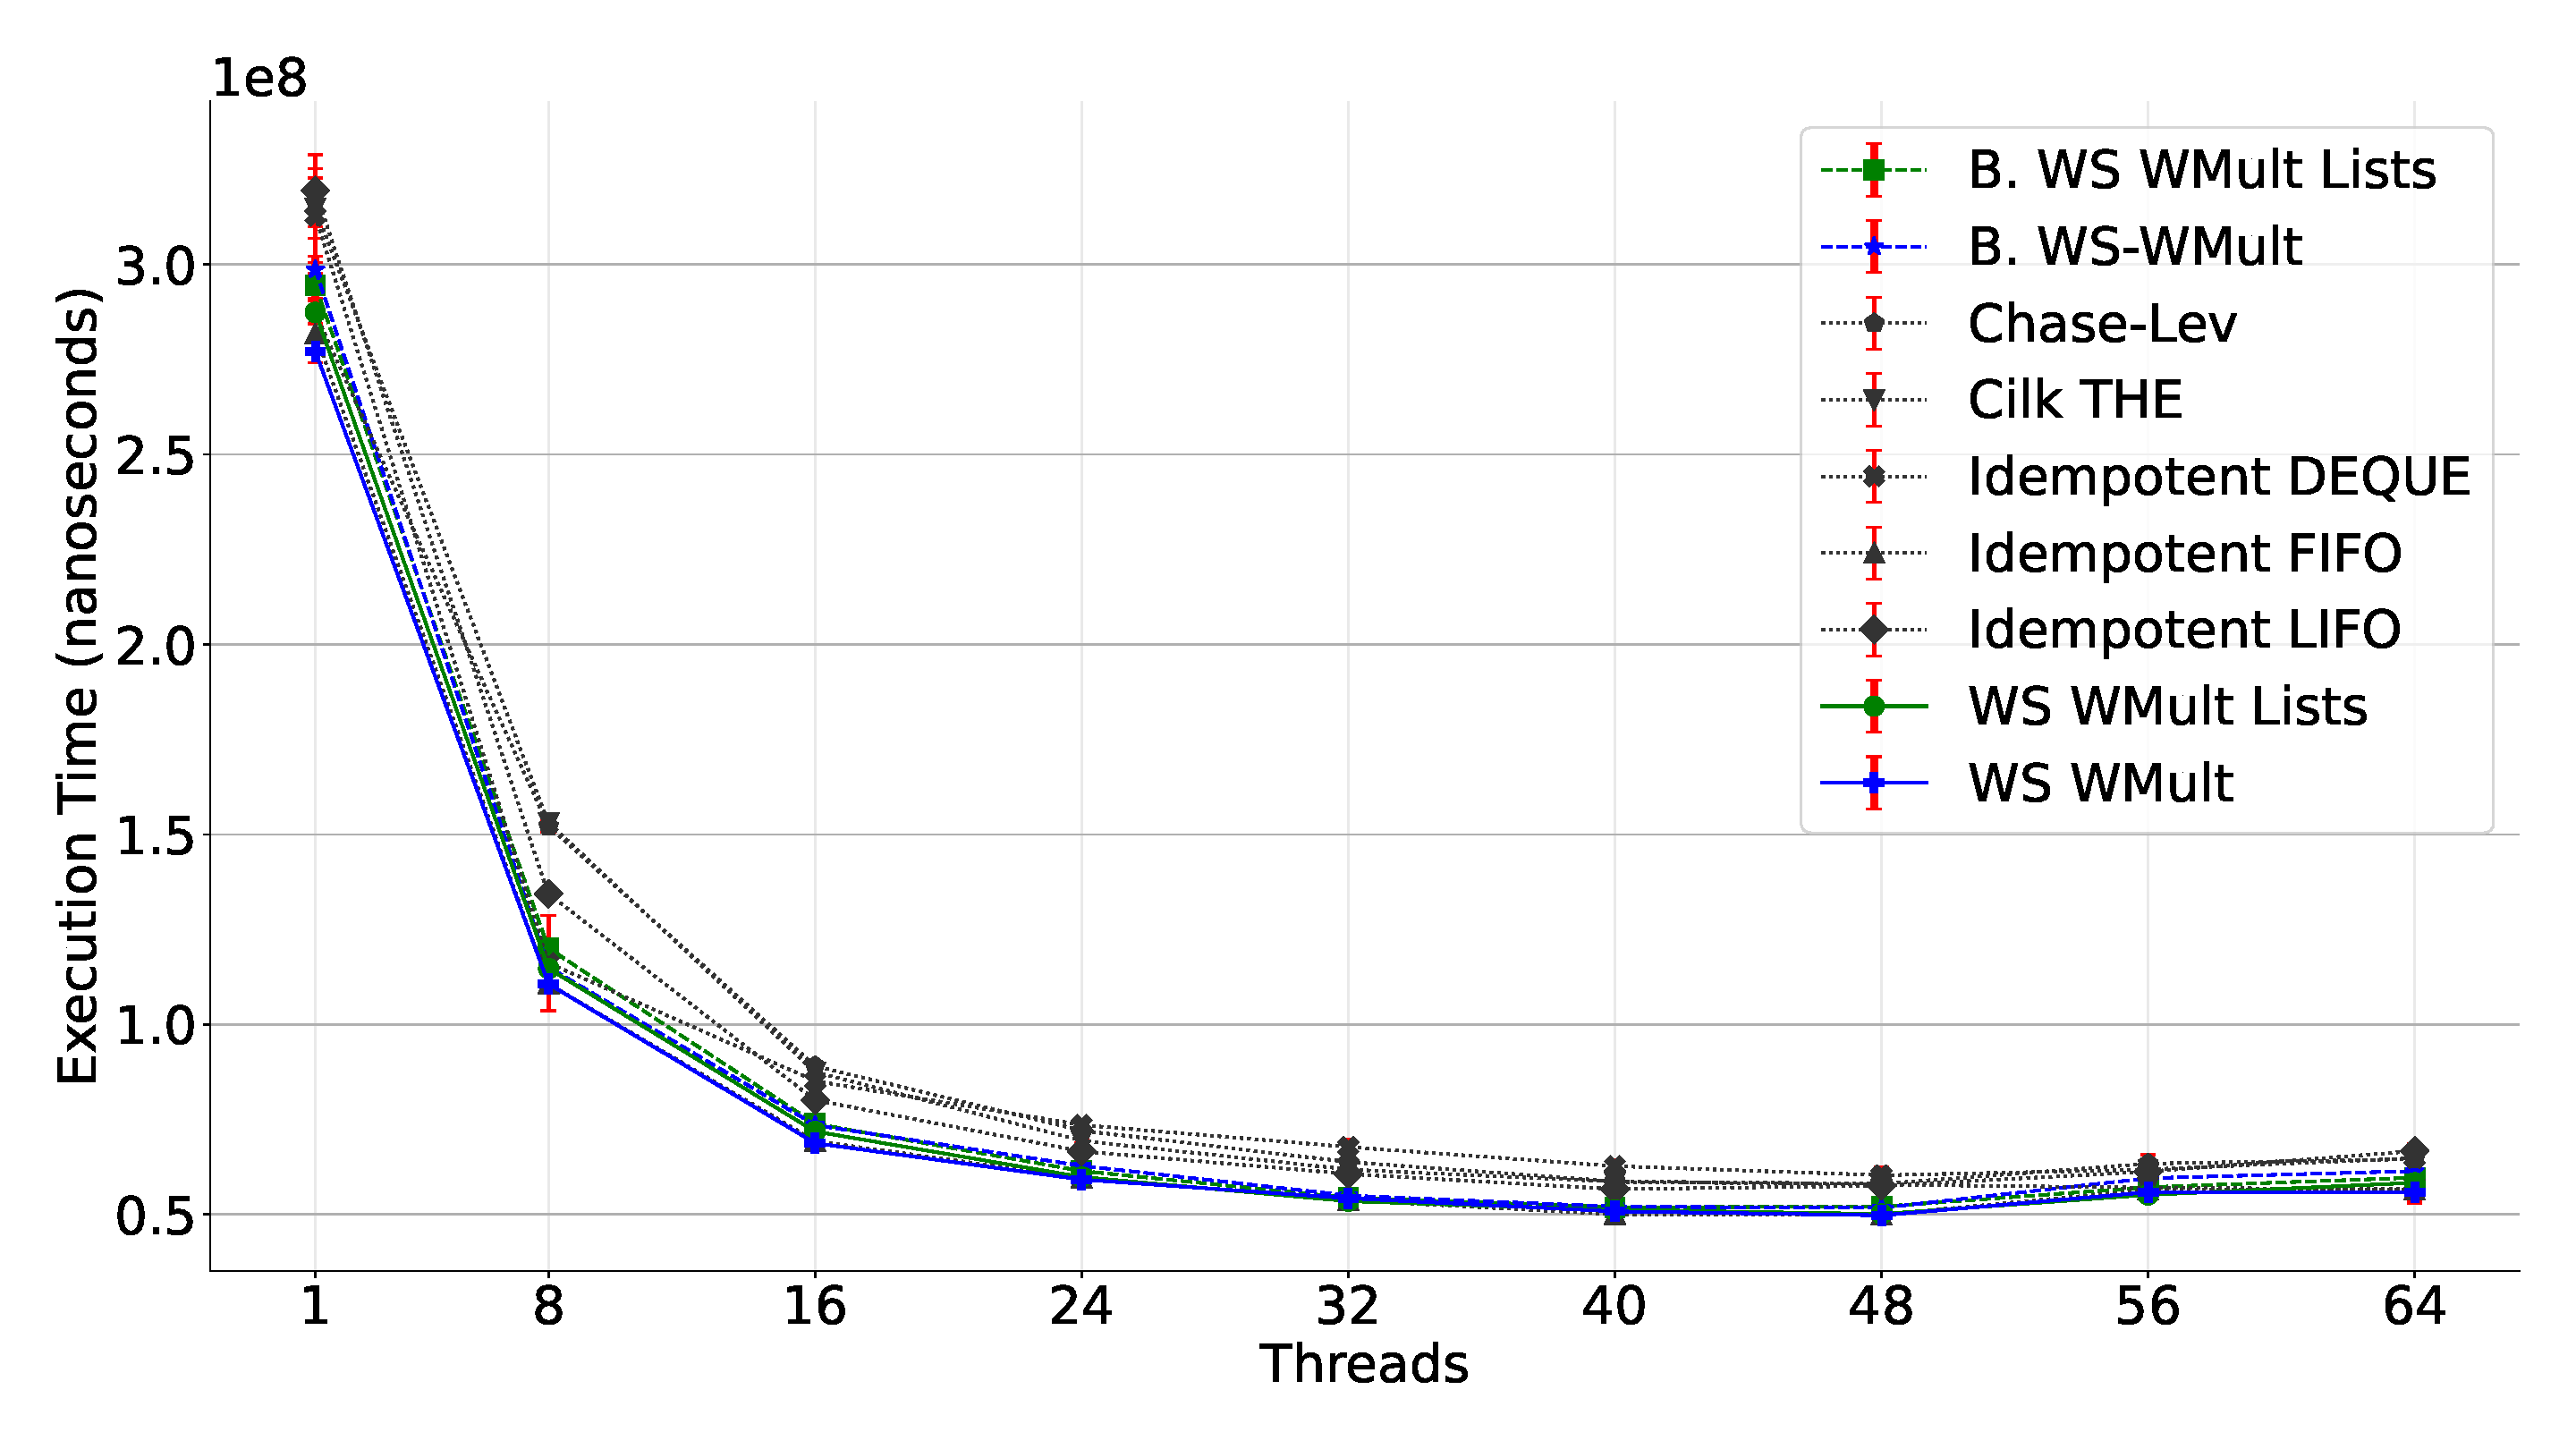
\includegraphics[width=0.48\textwidth]{contents/backmatter/evaluation/mean-TORUS3D40-Directed-256.pdf}
  }
  \qquad
  \subfloat[\label{fig:directed_torus3d40_1M} Mean times for the graph
  application benchmark. These are the results of the 3D Torus 40\%
  Directed graph. For each work-stealing algorithm's
  data structure, it begins its execution with an initial size of the benchmark.
  Each algorithm begins execution with an initial size of
  1,000,000 entries.] {
    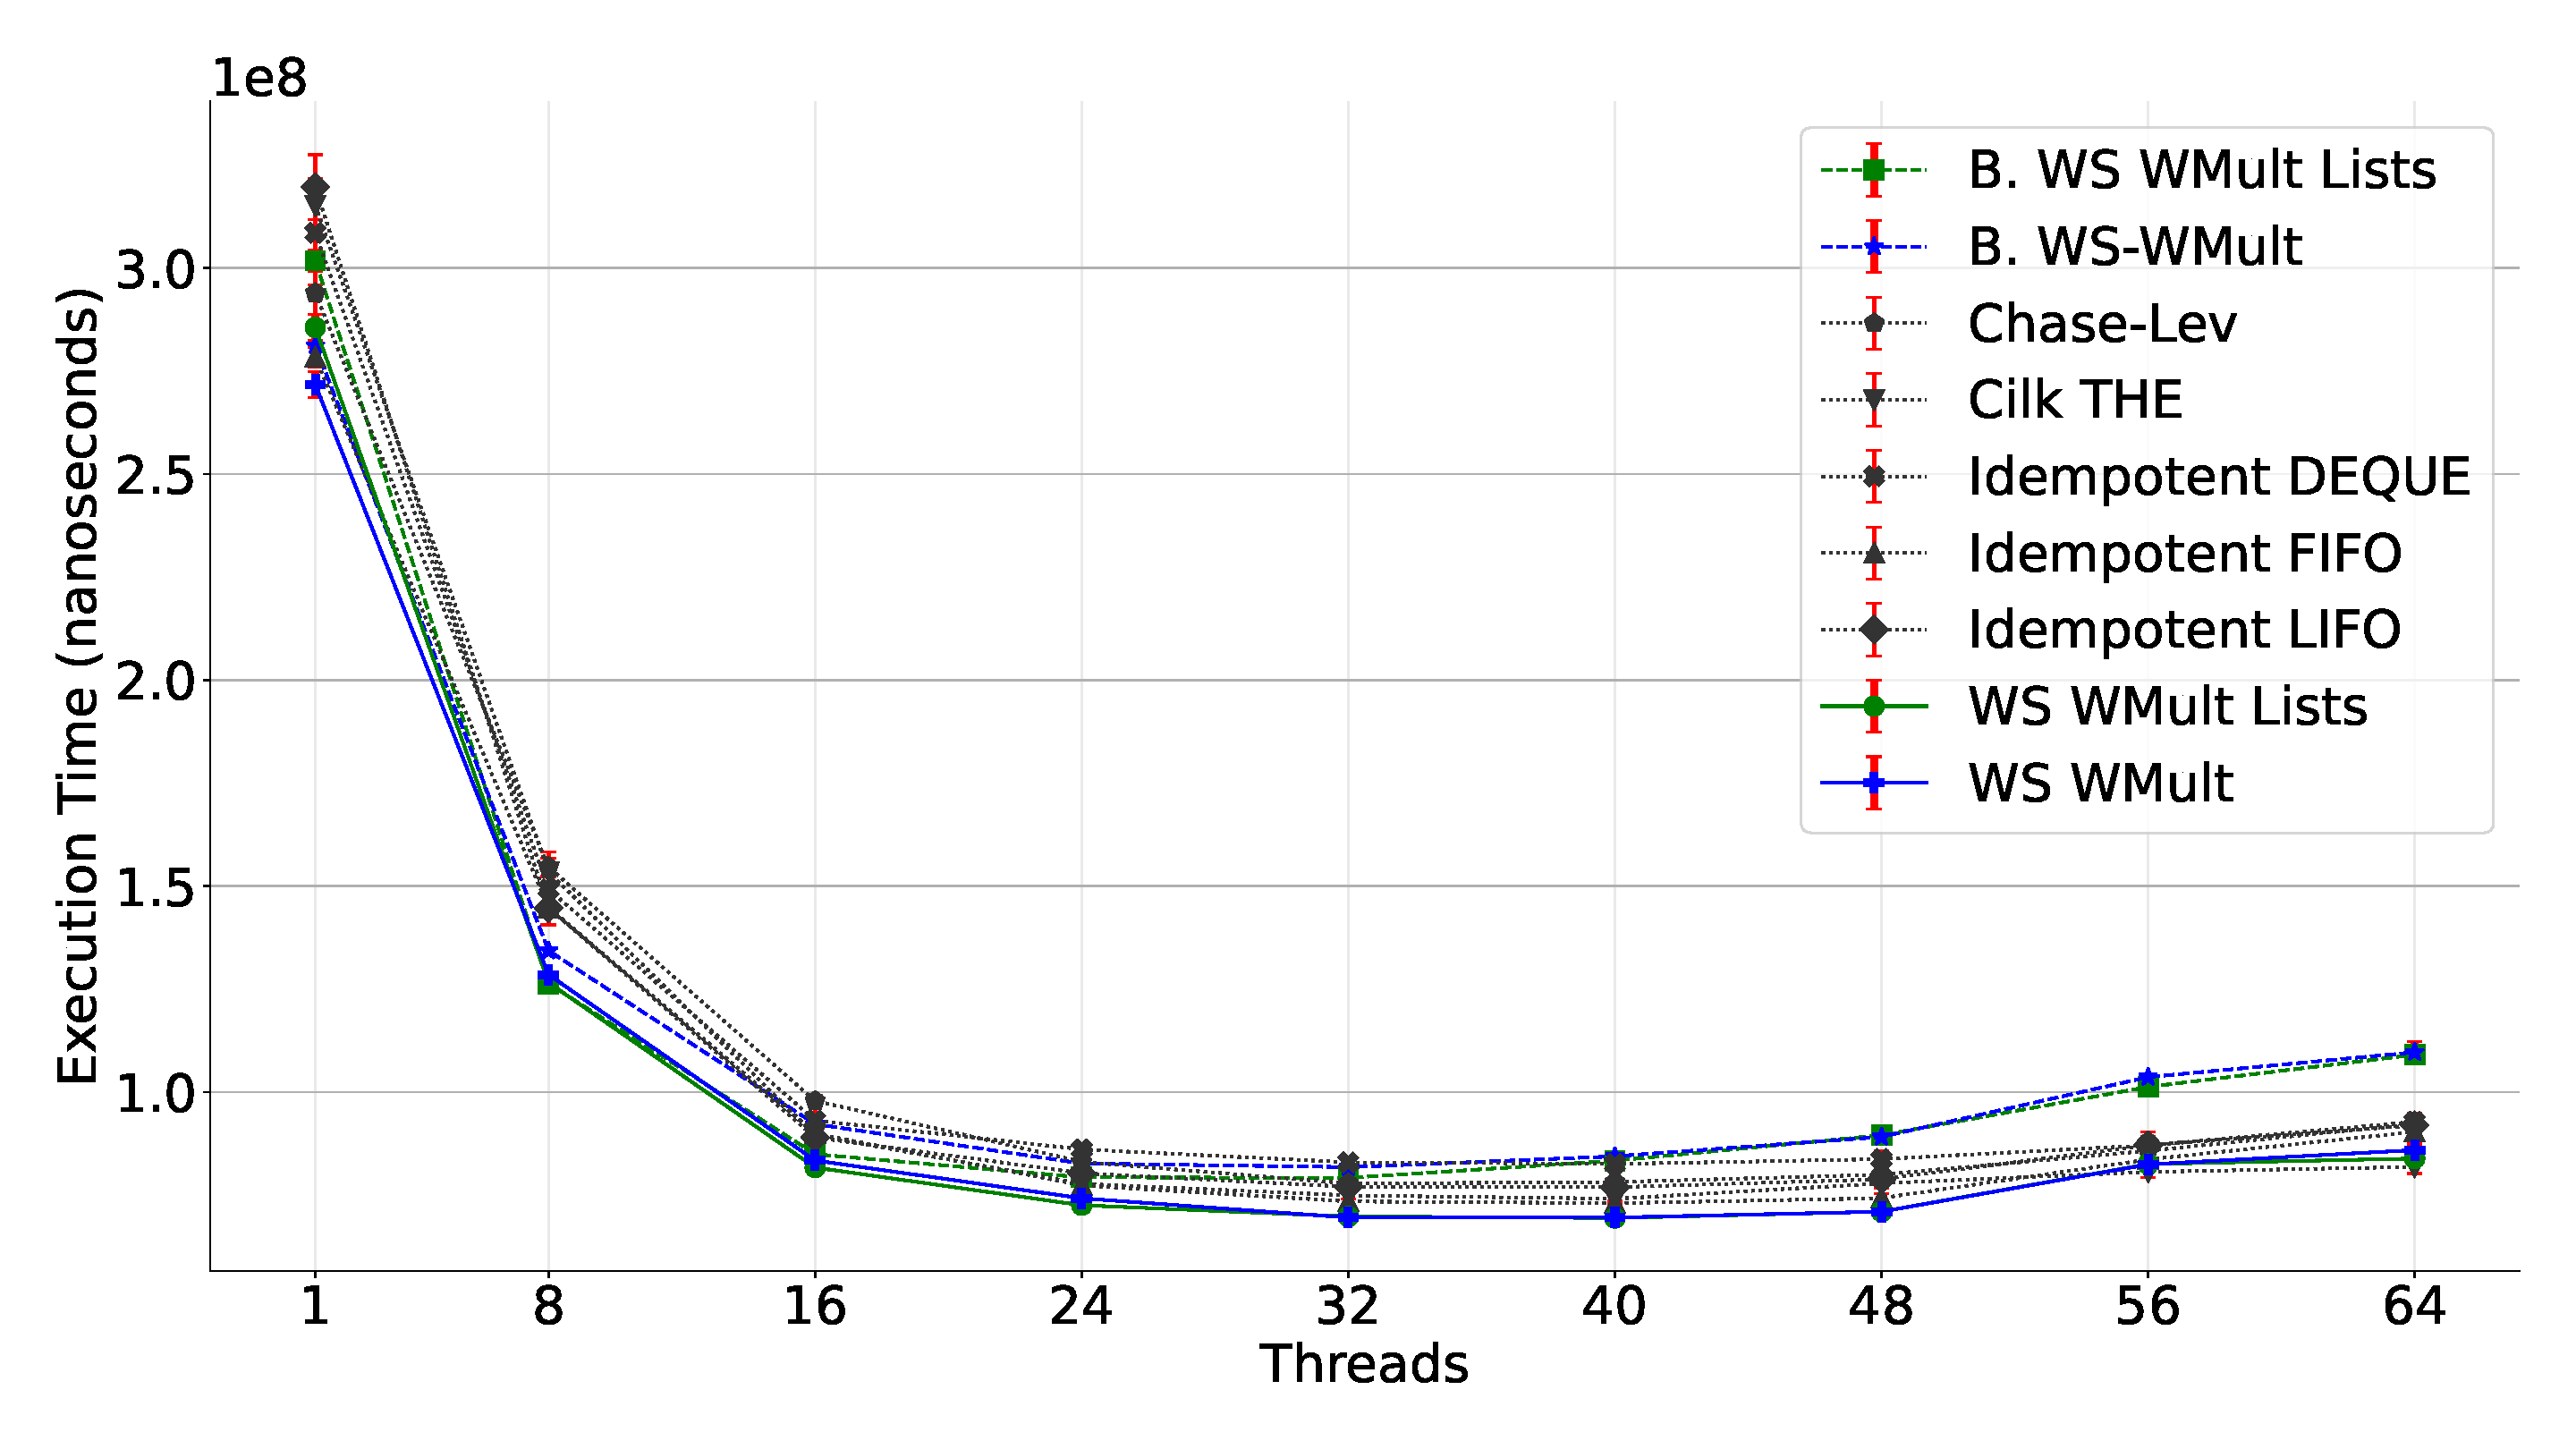
\includegraphics[width=0.48\textwidth]{contents/backmatter/evaluation/mean-TORUS3D40-Directed-1000000.pdf}
  }

  \subfloat[\label{fig:undirected_torus3d40_256} Mean times for the graph
  application benchmark. These are the results of the 3D Torus 40\%
  Undirected graph. For each work-stealing algorithm's
  data structure, it begins its execution with an initial size of
  the benchmark.  Each algorithm begins execution with an initial size of
  256 entries.] {
    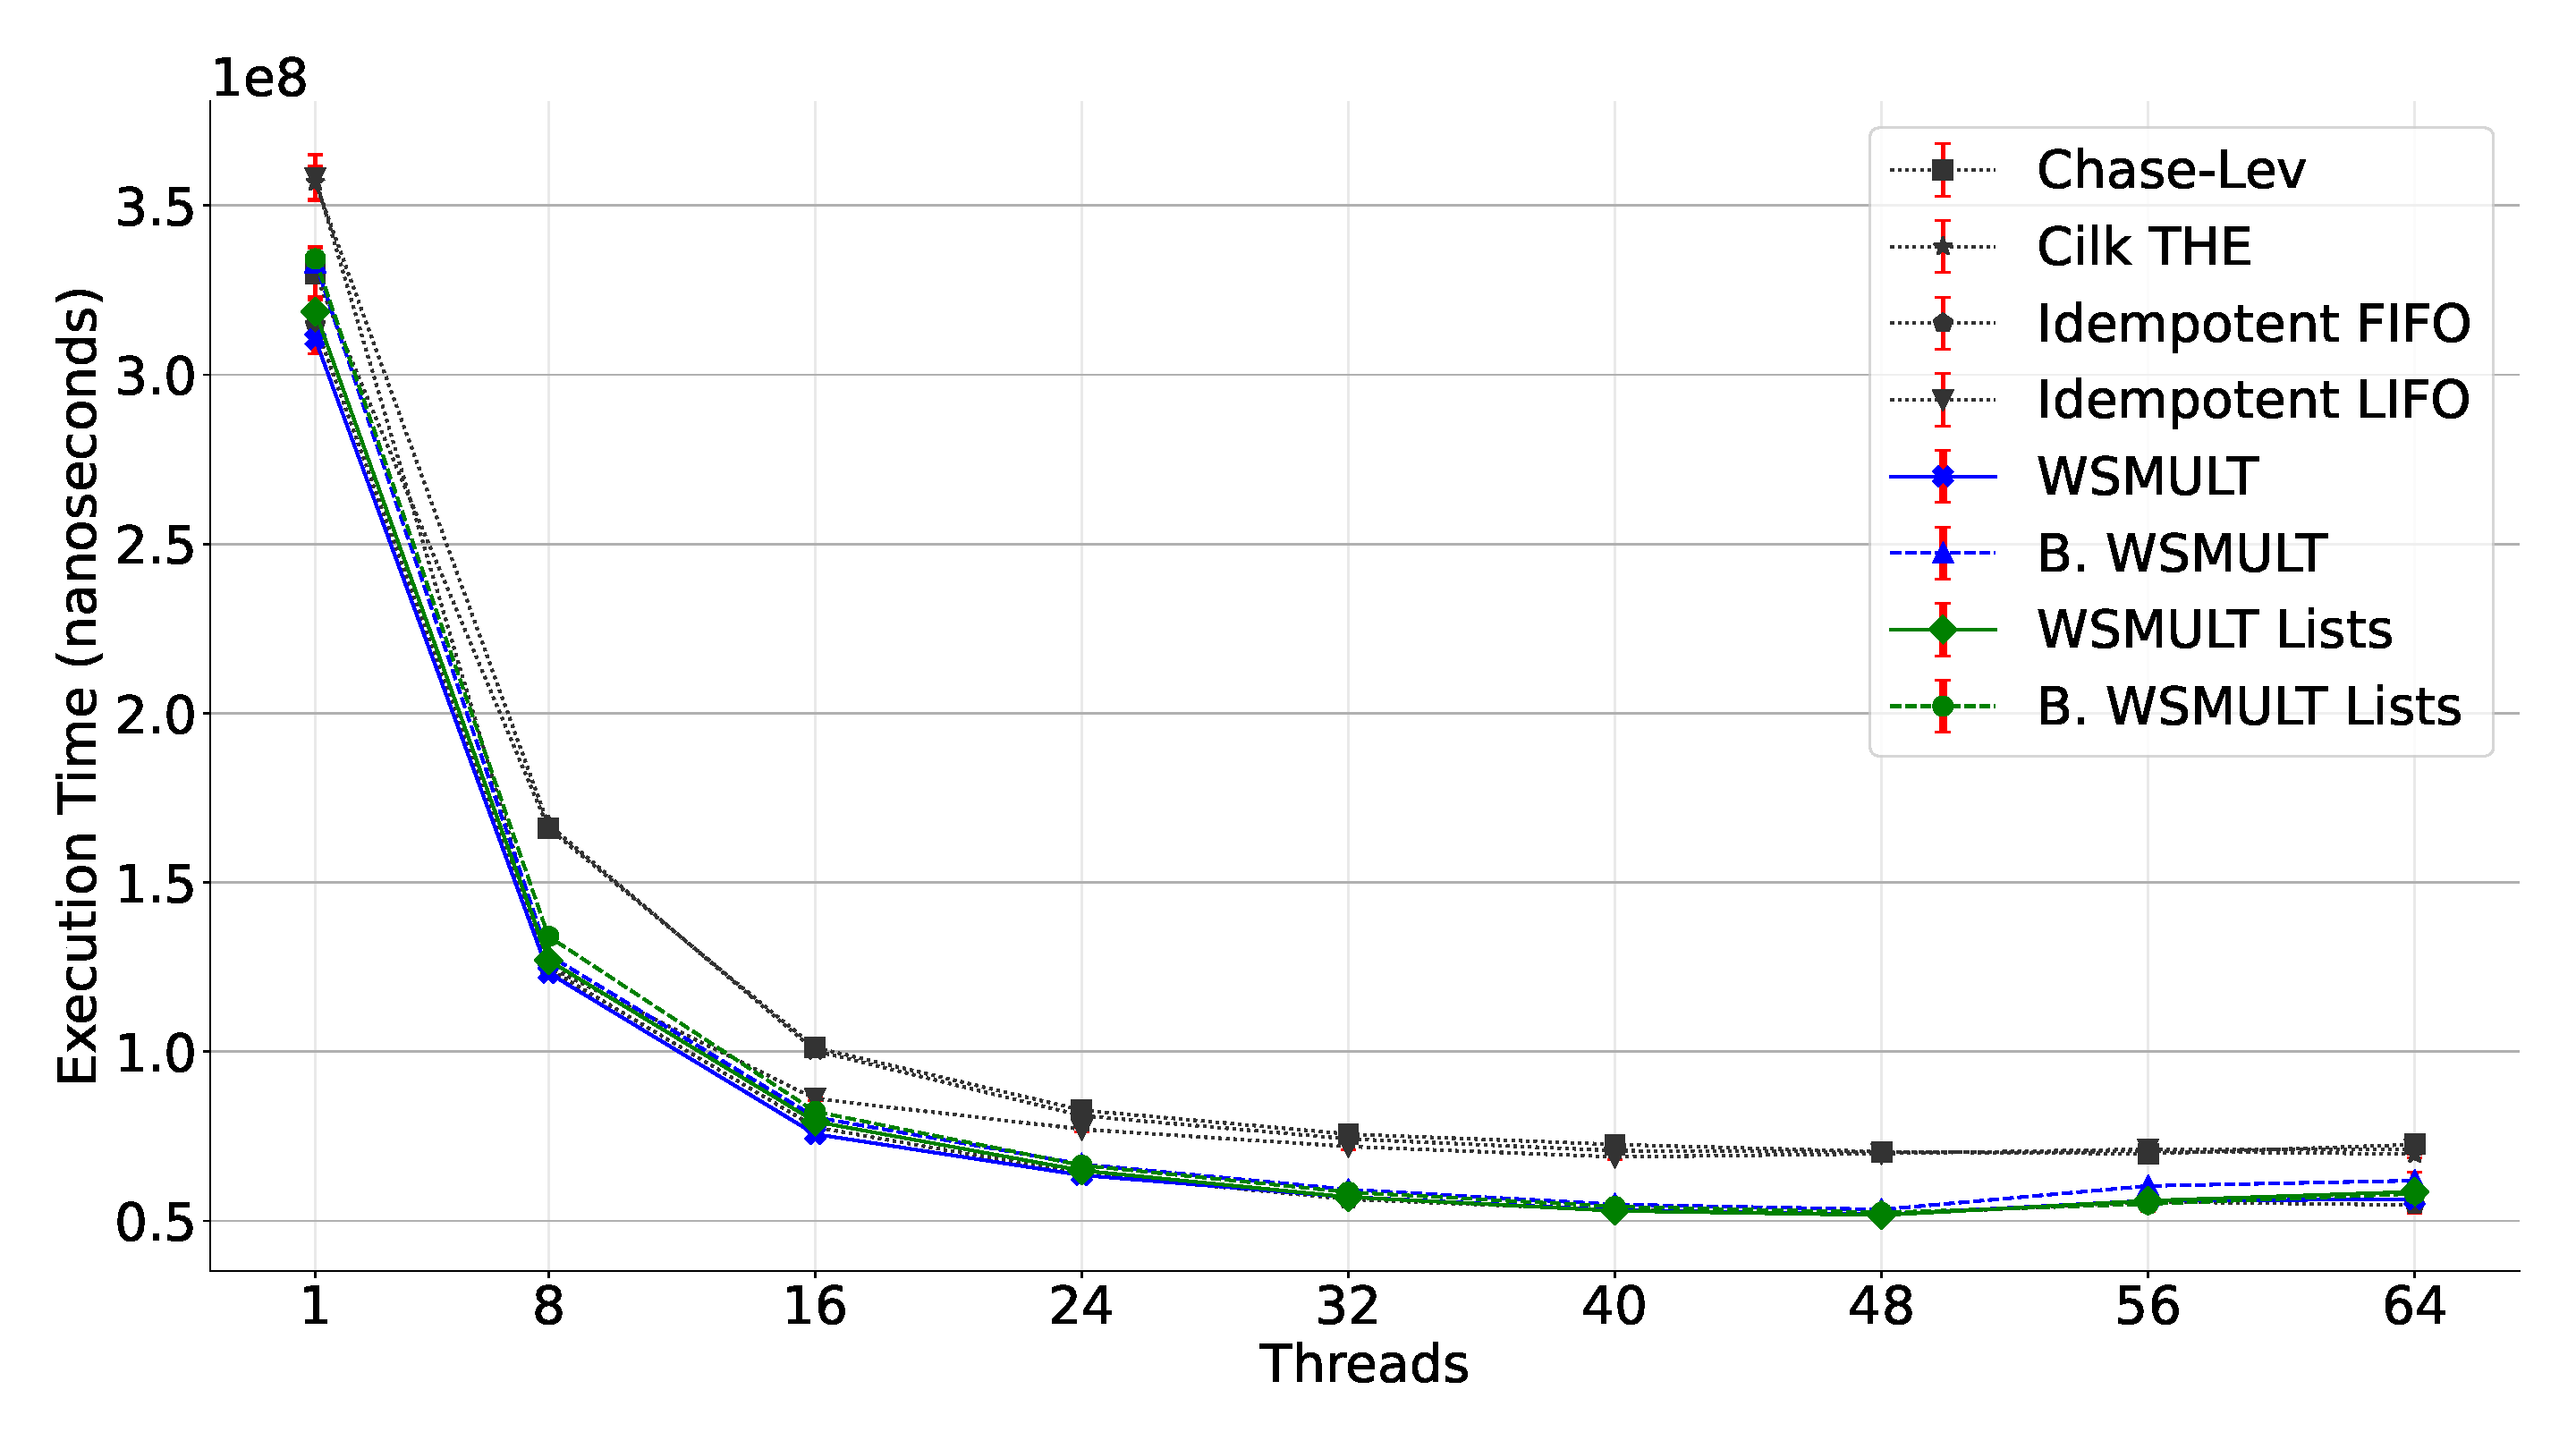
\includegraphics[width=0.48\textwidth]{contents/backmatter/evaluation/mean-TORUS3D40-Undirected-256.pdf}
  }
  \qquad
  \subfloat[\label{fig:undirected_torus3d40_1M} Mean times for the graph
  application benchmark. These are the results of the 3D Torus 40\%
  Undirected graph. For each work-stealing algorithm's
  data structure, it begins its execution with an initial size of
  the benchmark.  Each algorithm begins execution with an initial size of
  1,000,000 entries.] {
    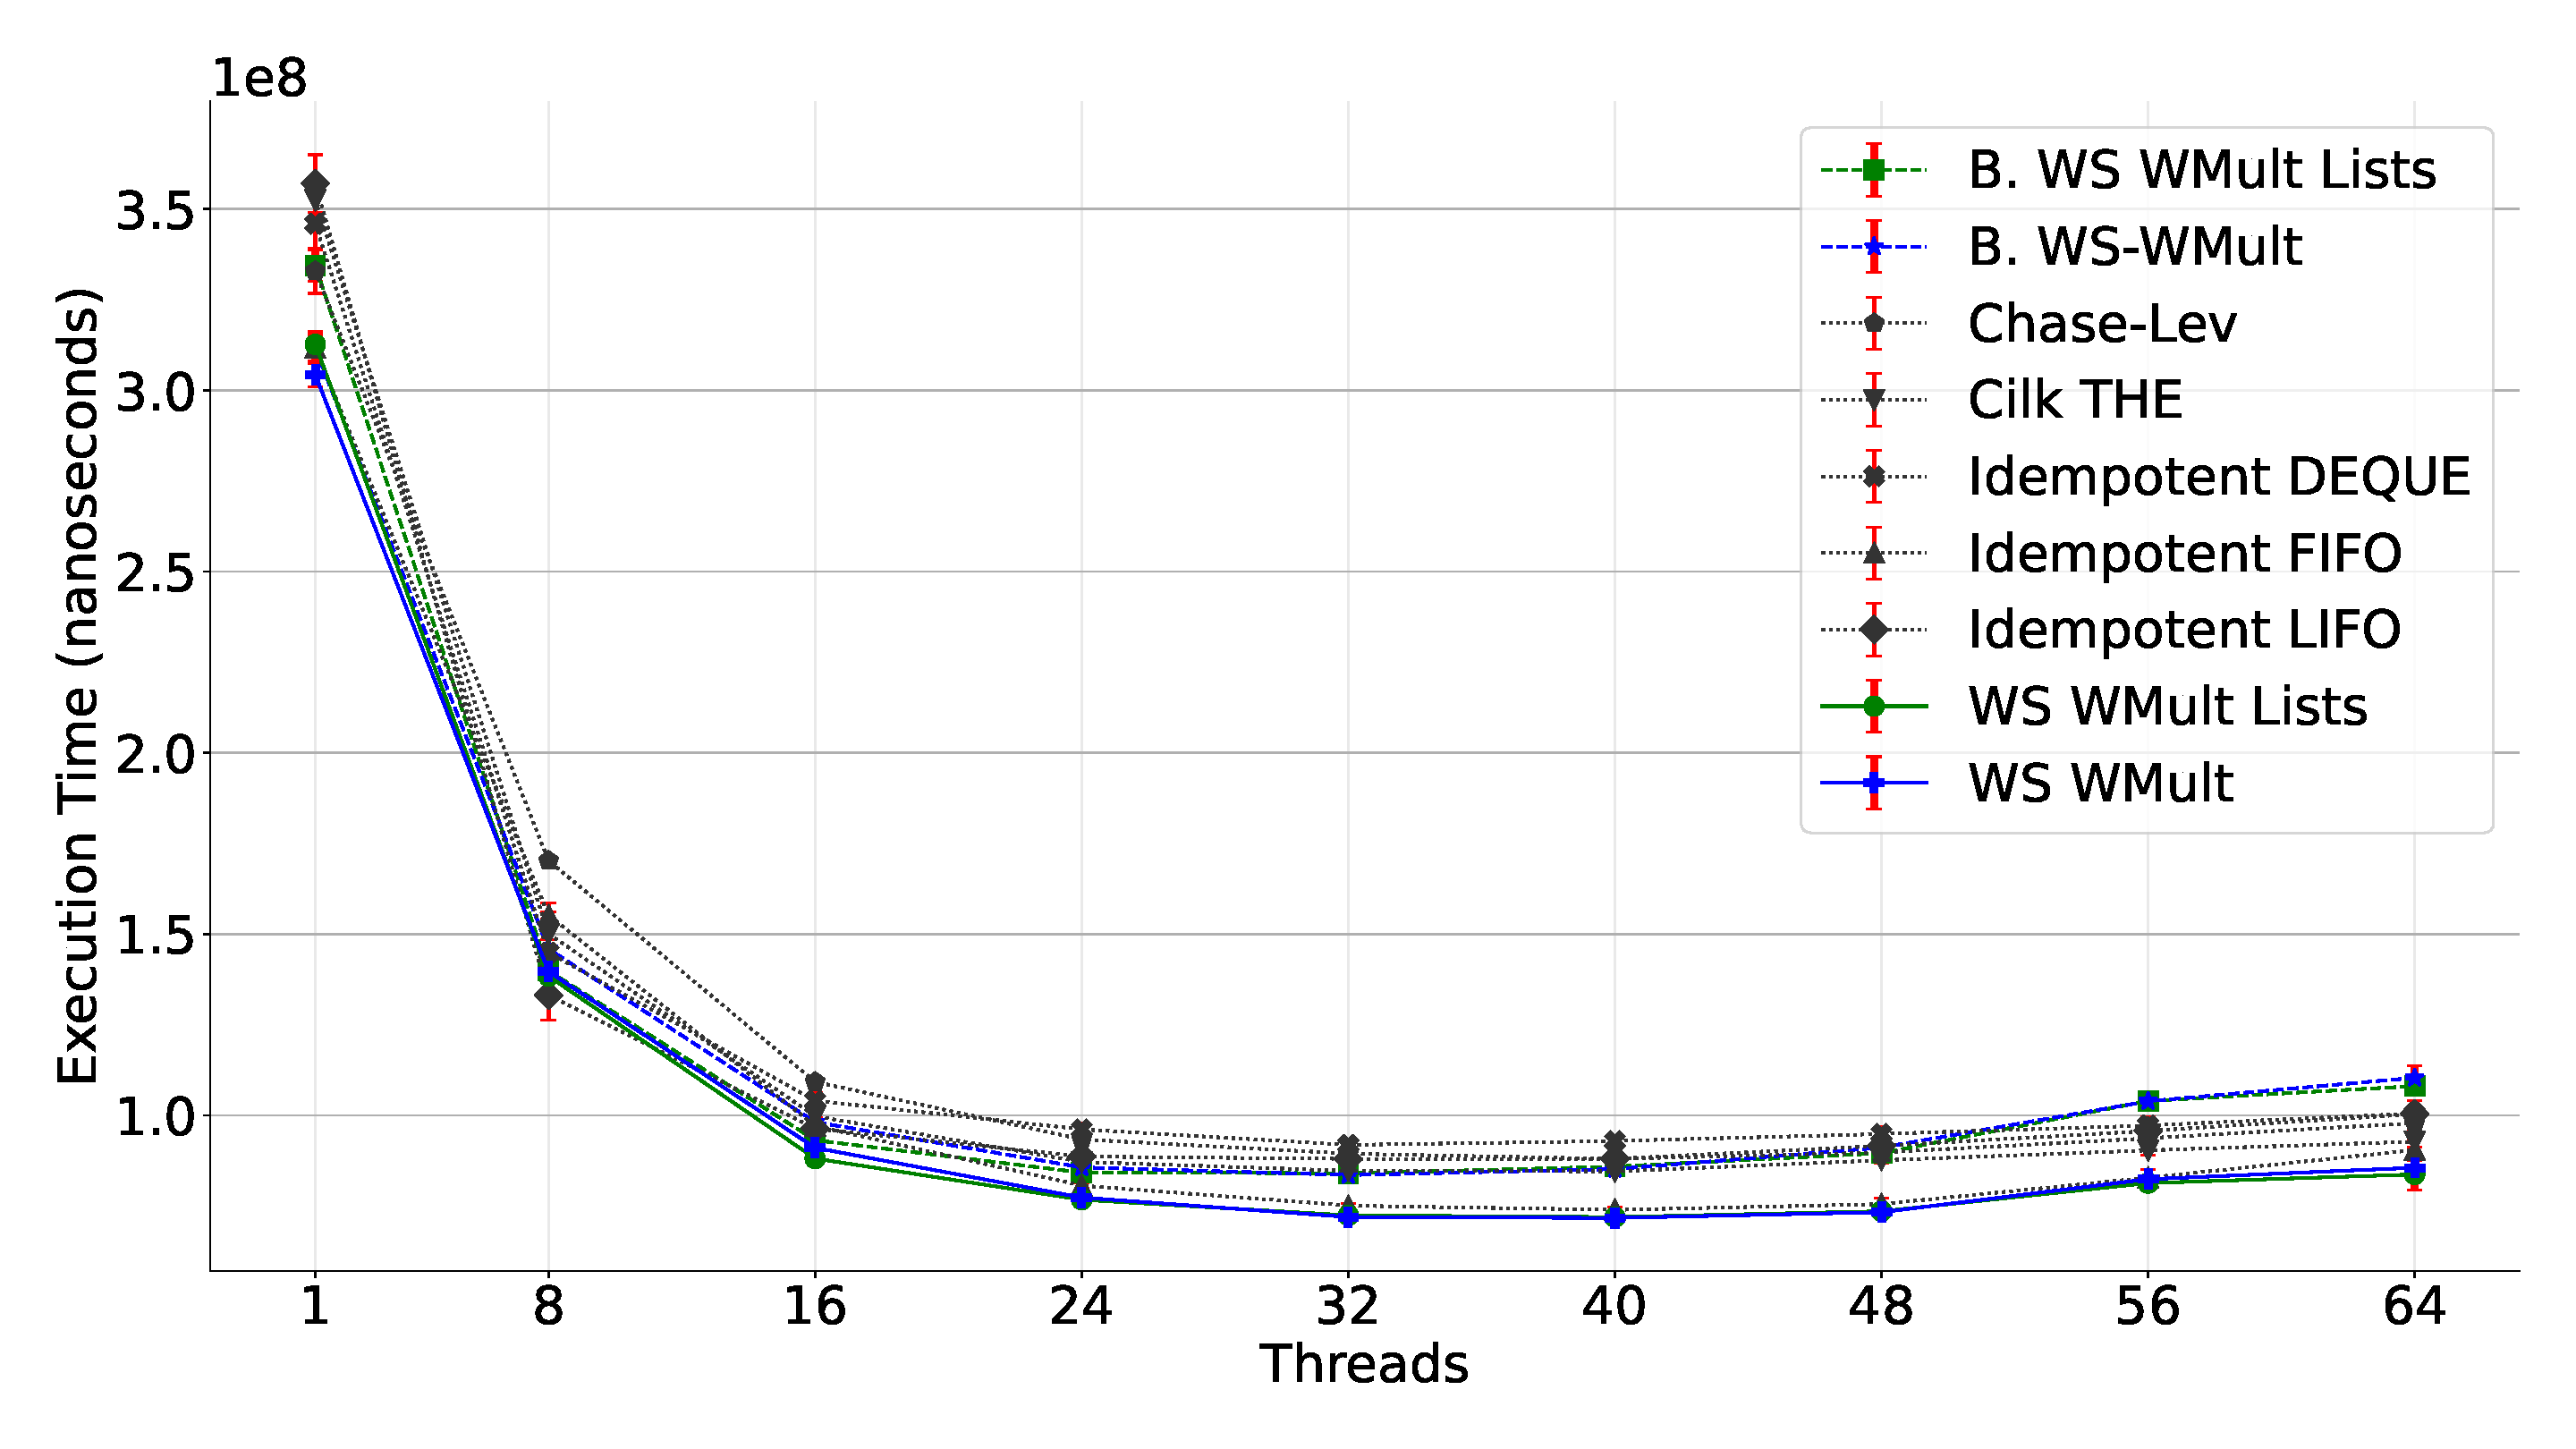
\includegraphics[width=0.48\textwidth]{contents/backmatter/evaluation/mean-TORUS3D40-Undirected-1000000.pdf}
  }
  \caption{\label{fig:3d40_torus_appendix} 3D Torus 40\% Directed and
    Undirected Graph with 256 and 1,000,000 initial sizes respectively.}
\end{figure}

\begin{table}[!ht]
\centering
\resizebox{\textwidth}{!}{\begin{tabular}{lrrrrrrrrr}
\toprule{} &           1  &           8  &          16 &          24 &          32 &          40 &          48 &          56 &          64 \\
\midrule
\textbf{B. WS WMult Lists} & 294432517.37 & 120021425.55 & 73823501.16 & 61390038.43 & 54354181.95 & 51833900.64 & 52023575.33 & 57131362.05 & 59648865.02 \\
\textbf{B. WS WMult      } & 298663678.64 & 115054783.47 & 73453047.11 & 62747462.27 & 54920691.10 & 52001289.43 & 51681136.53 & 59499980.10 & 61377477.24 \\
\textbf{Chase-Lev        } & 287240600.88 & 152115465.89 & 89012227.38 & 72023688.99 & 63761750.39 & 58658047.86 & 58004155.86 & 63342223.89 & 64548293.28 \\
\textbf{Cilk THE         } & 314871019.02 & 153049093.83 & 87438645.82 & 69353428.09 & 61776800.67 & 58530855.79 & 57804129.29 & 56974132.59 & 56592253.73 \\
\textbf{Idempotent DEQUE } & 312830298.62 & 116142320.22 & 85066483.24 & 73484481.82 & 67703602.98 & 62678789.22 & 60261928.04 & 61803224.08 & 64834634.28 \\
\textbf{Idempotent FIFO  } & 281784801.76 & 110651097.78 & 69253386.17 & 59583683.11 & 53682754.00 & 49991330.61 & 49891748.90 & 56450615.25 & 56486785.18 \\
\textbf{Idempotent LIFO  } & 319435336.99 & 134334876.65 & 80042328.23 & 66562292.68 & 60604520.16 & 56610182.19 & 57532942.70 & 61246247.57 & 66680269.13 \\
\textbf{WS WMult Lists   } & 287387470.69 & 114685026.00 & 71794869.08 & 59806522.26 & 53452614.01 & 51173585.38 & 50070658.75 & 55112170.91 & 58297658.11 \\
\textbf{WS WMult         } & 277155350.79 & 110607845.40 & 68713507.66 & 59139515.09 & 54219708.89 & 50765966.96 & 49719089.51 & 55809517.26 & 55806848.41 \\
\bottomrule
\end{tabular}}

\caption{\label{graph-TORUS3D40-Directed-256}Mean times for the graph application
    benchmark. These are the results for the 3D Torus 40\% Directed graph. Each
    algorithm begins its execution with an initial size of 256
    items.}
\end{table}

\begin{table}[!ht]
\centering
\resizebox{\textwidth}{!}{\begin{tabular}{lrrrrrrrrr}
\toprule{} &           1  &           8  &          16 &          24 &          32 &          40 &          48 &           56 &           64 \\
\midrule
\textbf{B. WS WMult Lists} & 301763957.74 & 126292839.15 & 84887857.49 & 79272185.13 & 79154954.71 & 83335257.72 & 89510324.32 & 101238037.04 & 109048106.48 \\
\textbf{B. WS WMult      } & 281186009.17 & 134302281.87 & 92202552.27 & 82636217.31 & 81748787.41 & 84392048.40 & 89105290.52 & 103621912.52 & 109658658.31 \\
\textbf{Chase-Lev        } & 293916625.21 & 154585238.00 & 97856281.89 & 83025587.50 & 77807388.15 & 78126159.57 & 79948552.74 &  85725727.08 &  92310399.45 \\
\textbf{Cilk THE         } & 315191868.24 & 153424659.25 & 89517444.61 & 77694402.78 & 74875845.38 & 74071535.76 & 77838585.82 &  80591541.79 &  81821539.23 \\
\textbf{Idempotent DEQUE } & 308537573.96 & 149211106.90 & 93096120.06 & 86063667.52 & 82913118.38 & 82531620.54 & 83710627.36 &  87052170.00 &  92779273.54 \\
\textbf{Idempotent FIFO  } & 278383663.89 & 144757144.09 & 89903067.87 & 77336892.60 & 73423810.85 & 72991479.36 & 74251359.12 &  83638031.97 &  90377859.79 \\
\textbf{Idempotent LIFO  } & 319638620.35 & 144624689.59 & 88959163.63 & 80275708.29 & 76970703.88 & 76881719.75 & 78838337.38 &  87078149.69 &  91934674.19 \\
\textbf{WS WMult Lists   } & 285576627.83 & 126550275.57 & 81652075.25 & 72512300.43 & 69779523.11 & 69421029.67 & 70961813.29 &  82500795.31 &  83848751.96 \\
\textbf{WS WMult         } & 271697926.58 & 128486529.15 & 83368234.66 & 74191411.95 & 69519514.10 & 69521643.56 & 70943495.75 &  82417635.97 &  85894721.48 \\
\bottomrule
\end{tabular}}

\caption{\label{graph-TORUS3D40-Directed-1000000}Mean times for the graph application
    benchmark. These are the results for the 3D Torus 40\% Directed graph. Each
    algorithm begins its execution with an initial size of 1000000
    items.}
\end{table}

\begin{table}[!ht]
\centering
\resizebox{\textwidth}{!}{\begin{tabular}{lrrrrrrrrr}
\toprule{} &           1  &           8  &           16 &          24 &          32 &          40 &          48 &          56 &          64 \\
\midrule
\textbf{Chase-Lev      } & 329816027.99 & 166018668.00 & 101194304.00 & 82693813.55 & 75637331.26 & 72548609.15 & 70421774.27 & 69807147.69 & 72606679.43 \\
\textbf{Cilk THE       } & 356916317.95 & 167055350.86 & 100233817.43 & 81074173.36 & 74222943.72 & 70749147.75 & 70338848.18 & 70562136.49 & 69687049.08 \\
\textbf{Idempotent FIFO} & 314791538.27 & 124518727.11 &  77680336.73 & 63919327.65 & 56394746.44 & 53229205.73 & 51781643.96 & 55674948.38 & 54641531.71 \\
\textbf{Idempotent LIFO} & 358165273.94 & 125105689.07 &  86102533.77 & 77056873.00 & 71960543.09 & 68881040.65 & 69877008.87 & 71220489.02 & 71125362.10 \\
\textbf{WS WMULT         } & 310482623.44 & 123277866.27 &  75627540.46 & 63491941.48 & 57072664.51 & 53150879.35 & 51860315.85 & 55971221.94 & 56381071.13 \\
\textbf{B. WS WMULT      } & 333148110.98 & 128544299.77 &  80629725.80 & 66742869.48 & 59245808.63 & 54831212.23 & 53350917.70 & 60339368.99 & 61904545.78 \\
\textbf{WS WMULT Lists   } & 318598312.42 & 126984605.65 &  79327818.59 & 64873208.49 & 57030534.60 & 52973456.00 & 51696004.73 & 55958368.16 & 58612461.28 \\
\textbf{B. WS WMULT Lists} & 334232009.92 & 134058201.59 &  82287300.73 & 66418704.09 & 58477222.64 & 54223431.95 & 52443567.62 & 55004602.31 & 58013627.62 \\
\bottomrule
\end{tabular}}

\caption{\label{graph-3D-Torus-40-undirected-256}Mean times for the graph application
    benchmark. These are the results for the 3D Torus 40\% Undirected graph. Each
    algorithm begins its execution with an initial size of 256
    items.}
\end{table}

\begin{table}[!ht]
\centering
\resizebox{\textwidth}{!}{\begin{tabular}{lrrrrrrrrr}
\toprule{} &           1  &           8  &           16 &          24 &          32 &          40 &          48 &           56 &           64 \\
\midrule
\textbf{B. WS WMult Lists} & 334464593.22 & 139869441.62 &  93118738.82 & 84202596.98 & 83980353.63 & 85865325.35 & 89570045.81 & 103955321.31 & 108082353.61 \\
\textbf{B. WS WMult      } & 311579693.68 & 145881522.20 &  98130498.61 & 85629026.30 & 83509625.99 & 85149457.30 & 91105762.40 & 103885268.05 & 110346559.14 \\
\textbf{Chase-Lev        } & 332908360.24 & 170224669.95 & 109220232.75 & 93343788.98 & 89389033.42 & 87979103.86 & 89744702.88 &  93698982.84 &  97875180.09 \\
\textbf{Cilk THE         } & 352562123.61 & 150060951.66 &  99760520.74 & 87126086.44 & 84656500.65 & 84533702.71 & 87602278.89 &  90333960.91 &  92750637.97 \\
\textbf{Idempotent DEQUE } & 345947619.04 & 144885937.88 & 104036420.18 & 96097964.76 & 91840290.82 & 92917394.80 & 94867142.72 &  97202251.38 & 100523216.90 \\
\textbf{Idempotent FIFO  } & 311553075.87 & 155166420.27 &  97058448.94 & 80591951.38 & 75066314.78 & 73895334.04 & 75520212.03 &  82801873.16 &  90442958.12 \\
\textbf{Idempotent LIFO  } & 357016153.83 & 133154299.38 &  96322449.36 & 88612359.68 & 87952279.63 & 88014320.73 & 91586087.90 &  95690280.32 & 100364216.97 \\
\textbf{WS WMult Lists   } & 312648264.91 & 138383488.50 &  88072075.50 & 76709536.59 & 72390868.09 & 71909451.21 & 73524758.08 &  81289669.58 &  83682658.43 \\
\textbf{WS WMult         } & 304293026.00 & 139635085.90 &  91022803.16 & 77301315.95 & 71943494.11 & 71677604.62 & 73267315.81 &  82367515.38 &  85539771.68 \\
\bottomrule
\end{tabular}}

\caption{\label{graph-TORUS3D40-Undirected-1000000}Mean times for the graph application
    benchmark. These are the results for the 3D Torus 40\% Undirected graph. Each
    algorithm begins its execution with an initial size of 1000000
    items.}
\end{table}



\begin{figure}[!ht]
  \subfloat[\label{fig:directed_random_256} Mean times for the graph
  application benchmark. These are the results of the Random
  Directed graph. For each work-stealing algorithm's
  data structure, it begins its execution with an initial size of
  the benchmark.  Each algorithm begins execution with an initial size of
  256 entries.] {
    \includegraphics[width=0.48\textwidth]{contents/backmatter/evaluation/mean-Random-Directed-256.pdf}
  }
  \qquad
  \subfloat[\label{fig:directed_random_1M}  Mean times for the graph
  application benchmark. These are the results of the Random
  Directed graph. For each work-stealing algorithm's
  data structure, it begins its execution with an initial size of
  the benchmark.  Each algorithm begins execution with an initial size of
  256 entries.] {
    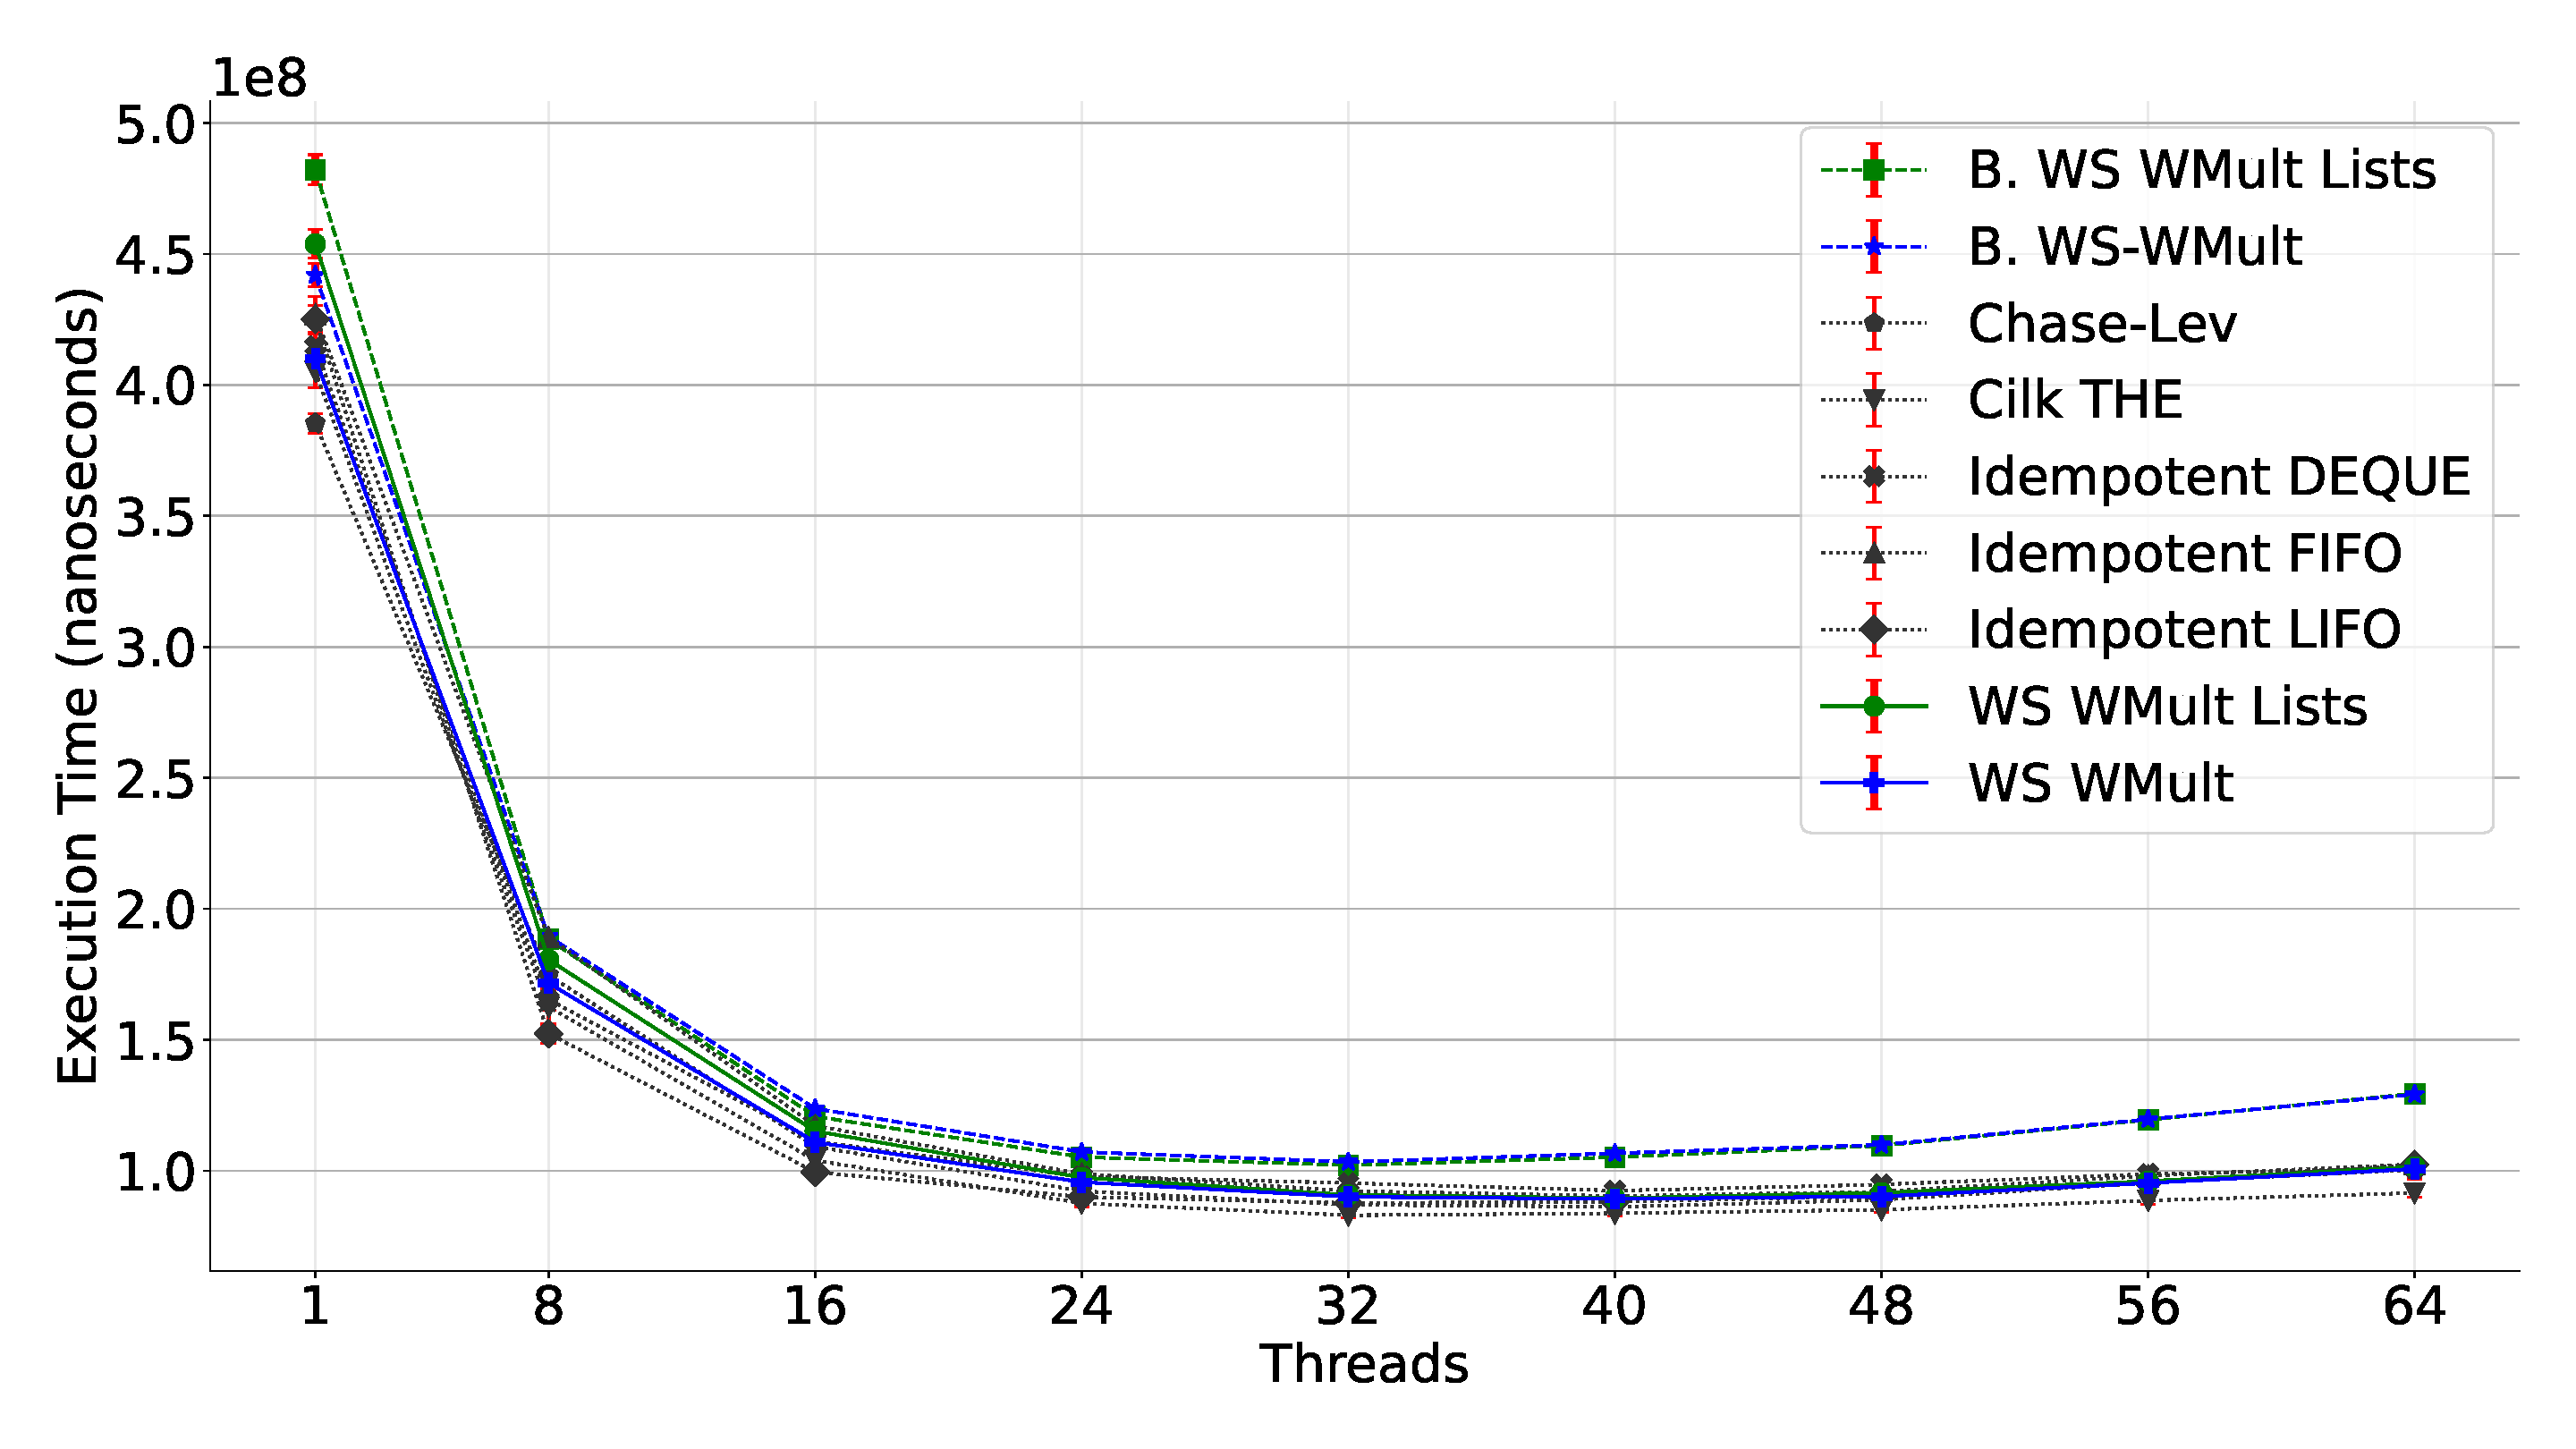
\includegraphics[width=0.48\textwidth]{contents/backmatter/evaluation/mean-RANDOM-Directed-1000000.pdf}
  }

  \subfloat[\label{fig:undirected_random_256} Mean times for the graph
  application benchmark. These are the results of the Random
  Directed graph. For each work-stealing algorithm's
  data structure, it begins its execution with an initial size of
  the benchmark.  Each algorithm begins execution with an initial size of
  256 entries.] {
    \includegraphics[width=0.48\textwidth]{contents/backmatter/evaluation/mean-Random-Undirected-256.pdf}
  }
  \qquad
  \subfloat[\label{fig:undirected_random_1M}  Mean times for the graph
  application benchmark. These are the results of the Random
  Undirected graph. For each work-stealing algorithm's
  data structure, it begins its execution with an initial size of
  the benchmark.  Each algorithm begins execution with an initial size of
  1,000,000 entries.] {
    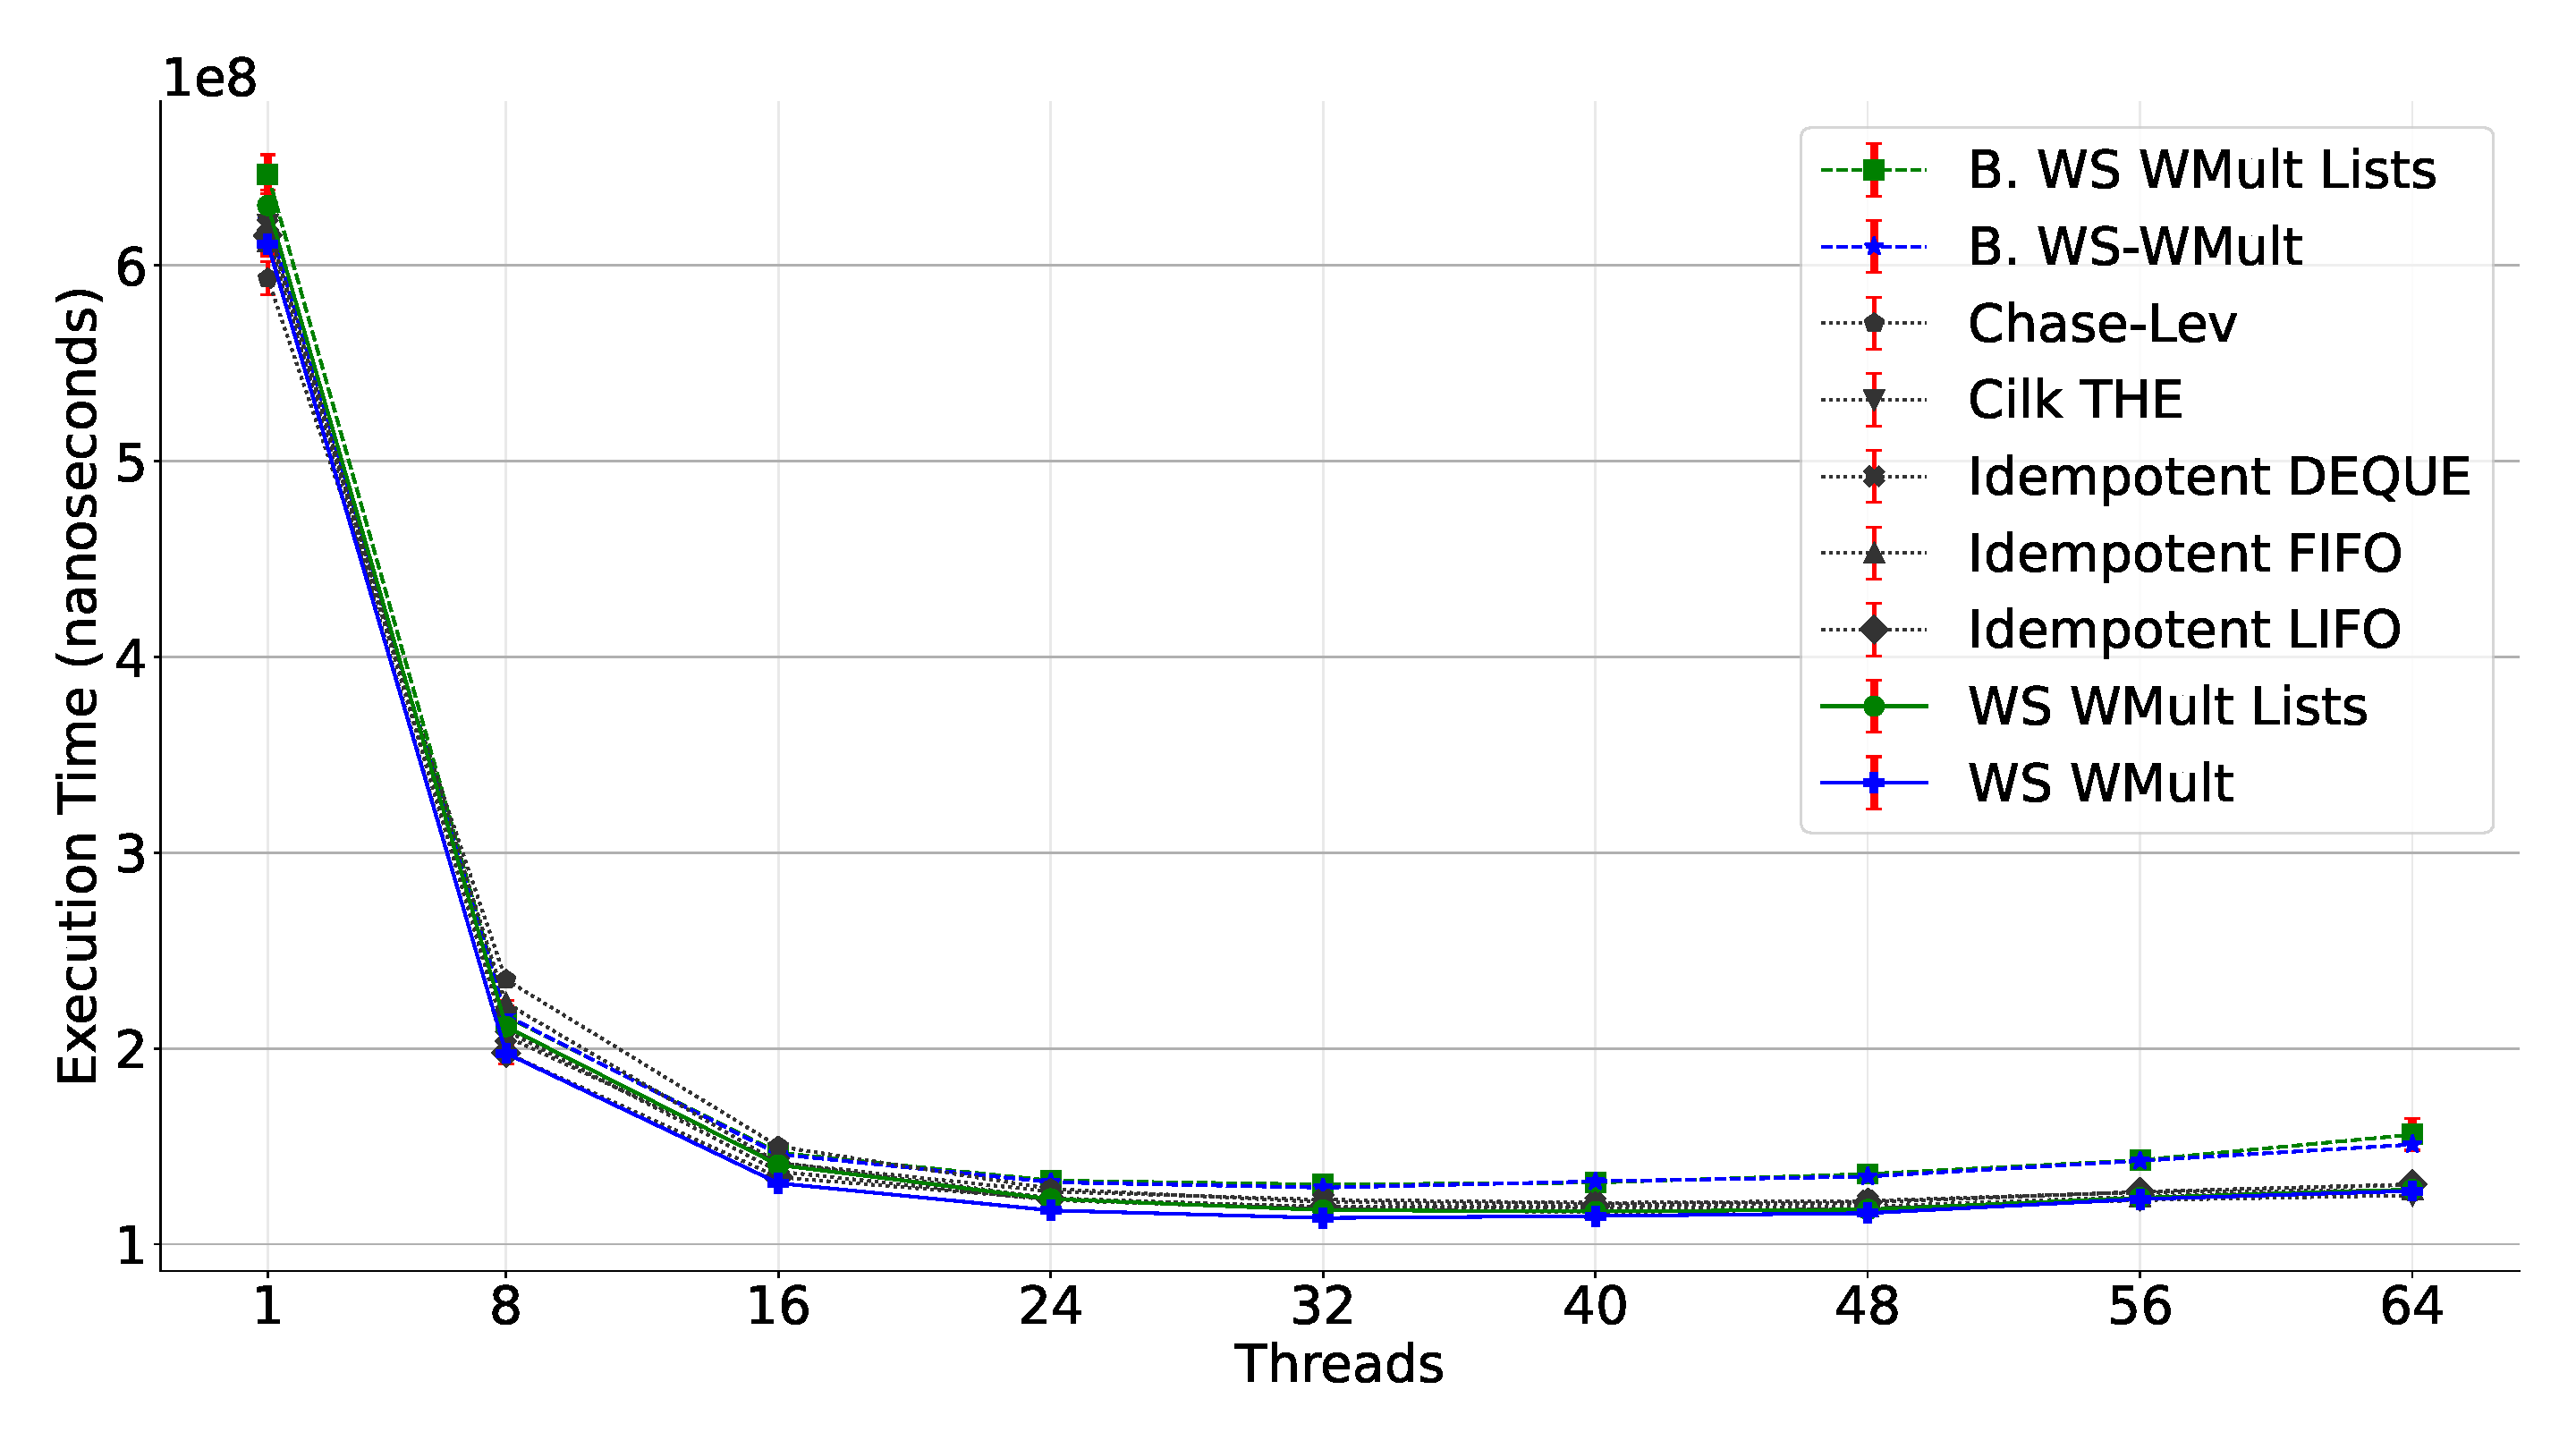
\includegraphics[width=0.48\textwidth]{contents/backmatter/evaluation/mean-RANDOM-Undirected-1000000.pdf}
  }
  \caption{\label{fig:random_appendix} Random Directed and
    Undirected Graph with 256 and 1,000,000 initial sizes
    respectively.}
\end{figure}

\input{contents/backmatter/evaluation/mean-Random-Directed-256.tex}
\begin{table}[!ht]
\centering
\resizebox{\textwidth}{!}{\begin{tabular}{lrrrrrrrrr}
\toprule{} &           1  &           8  &           16 &           24 &           32 &           40 &           48 &           56 &           64 \\
\midrule
\textbf{B. WS WMult Lists} & 482160068.48 & 188336095.42 & 120700826.52 & 105196857.53 & 102113641.09 & 105162929.44 & 109584170.31 & 119487423.69 & 129451320.56 \\
\textbf{B. WS WMult      } & 441884607.61 & 189459191.22 & 123728462.81 & 107166435.55 & 103353938.65 & 106676865.57 & 109881300.60 & 119661581.70 & 129178737.27 \\
\textbf{Chase-Lev        } & 385340577.40 & 174664858.65 & 109232027.31 &  92202519.86 &  87016638.92 &  86185560.86 &  88905638.86 &  95454735.65 & 100458140.05 \\
\textbf{Cilk THE         } & 405144969.95 & 162520672.80 & 103929415.16 &  87591486.16 &  83002578.54 &  83794041.85 &  85119207.59 &  88656720.05 &  91558486.63 \\
\textbf{Idempotent DEQUE } & 414733560.90 & 165342618.80 & 111167218.22 &  97768702.72 &  95273218.10 &  92395813.22 &  94765056.90 &  98724645.98 & 101022772.80 \\
\textbf{Idempotent FIFO  } & 426842811.31 & 189062631.20 & 117185450.64 &  98759795.45 &  92265610.82 &  90328848.01 &  92077270.18 &  98034222.72 & 102493646.11 \\
\textbf{Idempotent LIFO  } & 425017719.73 & 152344725.60 &  99461217.11 &  90006238.62 &  87681136.21 &  88206820.36 &  90283254.07 &  95488801.00 & 102316035.46 \\
\textbf{WS WMult Lists   } & 453825844.09 & 180552914.55 & 115121584.18 &  97398795.85 &  90786582.21 &  89502129.75 &  91607446.68 &  96029389.94 & 101519435.08 \\
\textbf{WS WMult         } & 409944339.41 & 171618034.92 & 110920773.91 &  95664656.10 &  90049503.96 &  89225431.26 &  90197459.73 &  95304067.23 & 100696398.66 \\
\bottomrule
\end{tabular}}

\caption{\label{graph-RANDOM-Directed-1000000}Mean times for the graph application
    benchmark. These are the results for the Random Directed graph. Each
    algorithm begins its execution with an initial size of 1000000
    items.}
\end{table}

\input{contents/backmatter/evaluation/mean-Random-Undirected-256.tex}
\begin{table}[!ht]
\centering
\resizebox{\textwidth}{!}{\begin{tabular}{lrrrrrrrrr}
\toprule{} &           1  &           8  &           16 &           24 &           32 &           40 &           48 &           56 &           64 \\
\midrule
\textbf{B. WS WMult Lists} & 646541284.19 & 216263265.20 & 146759280.43 & 132541176.53 & 130512193.85 & 131523019.65 & 135918877.69 & 142989655.30 & 156049348.80 \\
\textbf{B. WS WMult      } & 622923092.34 & 216837946.90 & 146021906.28 & 131696898.21 & 128922852.74 & 132160589.40 & 134643408.57 & 142655863.73 & 150954630.75 \\
\textbf{Chase-Lev        } & 593236904.85 & 235082293.49 & 149973065.80 & 128300559.06 & 121496061.31 & 120640561.49 & 121437035.74 & 126943494.15 & 130407001.13 \\
\textbf{Cilk THE         } & 620863347.51 & 209168448.86 & 137197146.35 & 122570308.33 & 117931034.32 & 116320400.08 & 118205988.97 & 122554842.13 & 125001132.55 \\
\textbf{Idempotent DEQUE } & 620533697.72 & 206167259.40 & 141569448.10 & 126905708.14 & 122788765.72 & 121143353.94 & 122235287.98 & 126617596.40 & 127807686.04 \\
\textbf{Idempotent FIFO  } & 611933226.01 & 223162610.33 & 141521019.59 & 123592991.13 & 118780262.20 & 118437149.38 & 119279944.51 & 124372070.49 & 127962219.33 \\
\textbf{Idempotent LIFO  } & 615205002.42 & 197693607.26 & 134245575.36 & 123088544.61 & 119117560.12 & 119495674.49 & 121411201.90 & 126847418.11 & 130739705.03 \\
\textbf{WS WMult Lists   } & 630514406.43 & 211180985.60 & 140475330.14 & 123174961.72 & 117468510.92 & 116733496.47 & 117762755.18 & 123778079.83 & 128006874.12 \\
\textbf{WS WMult         } & 610832074.69 & 197574834.99 & 131195696.62 & 117332821.11 & 113455313.17 & 114436181.30 & 115915780.99 & 123082517.02 & 127229090.01 \\
\bottomrule
\end{tabular}}

\caption{\label{graph-RANDOM-Undirected-1000000}Mean times for the graph application
    benchmark. These are the results for the Random Undirected graph. Each
    algorithm begins its execution with an initial size of 1000000
    items.}
\end{table}


\clearpage

\subsection{\label{subsec:repeated-work}Puts and takes performed in
  the Paralled Spanning Tree experiment}

This section reports the number of puts and takes performed during the
execution of the parallel spanning tree. This evaluation was performed
for each graph and all work-stealing algorithms. Additionally, the
difference between the total number of puts and the total number of
takes is calculated. Finally, the total surplus work is calculated as
the difference between the total put and the total available work
(number of vertices). For purposes of visualizing the amount of surplus
work, this is displayed as a graph in terms of the percentage of total
available work.

\subsubsection{Directed Torus 2D. Initial size of 256 items.}
\begin{table}[!ht]
\centering
\resizebox{\textwidth}{!}{\begin{tabular}{lrrrrrrrrrrrrrrr}
\toprule
\textbf{Algorithm} & \multicolumn{5}{l}{Chase-Lev} & \multicolumn{5}{l}{Cilk THE} & \multicolumn{5}{l}{Idempotent LIFO} \\
\textbf{Operation} &       Puts &      Takes & Difference (\%) & Surplus (\%) & Executed Surplus (\%) &       Puts &      Takes & Difference (\%) & Surplus (\%) & Executed Surplus (\%) &            Puts &      Takes & Difference (\%) & Surplus (\%) & Executed Surplus (\%) \\
\textbf{Processes} & \multicolumn{4}{l}{} & \multicolumn{4}{l}{} & \multicolumn{4}{l}{}\\ \midrule
\textbf{1 } & 1000000.00 & 1000000.00 &           0.00 &        0.00 &                 0.00 & 1000000.00 & 1000000.00 &           0.00 &        0.00 &                 0.00 &      1000000.00 & 1000000.00 &           0.00 &        0.00 &                 0.00 \\
\textbf{8 } & 1459383.80 & 1041490.20 &          28.63 &       31.48 &                 3.98 & 1033699.60 & 1000020.40 &           3.26 &        3.26 &                 0.00 &      1000583.40 & 1000241.00 &           0.03 &        0.06 &                 0.02 \\
\textbf{16} & 1448842.40 & 1033211.00 &          28.69 &       30.98 &                 3.21 & 1044556.60 & 1000118.60 &           4.25 &        4.27 &                 0.01 &      1001805.40 & 1000745.80 &           0.11 &        0.18 &                 0.07 \\
\textbf{24} & 1454352.20 & 1028947.20 &          29.25 &       31.24 &                 2.81 & 1041856.20 & 1000150.40 &           4.00 &        4.02 &                 0.02 &      1003160.00 & 1000912.80 &           0.22 &        0.32 &                 0.09 \\
\textbf{28} & 1433539.00 & 1022538.80 &          28.67 &       30.24 &                 2.20 & 1041198.80 & 1000140.00 &           3.94 &        3.96 &                 0.01 &      1002856.20 & 1000665.40 &           0.22 &        0.28 &                 0.07 \\
\textbf{32} & 1461140.80 & 1023658.80 &          29.94 &       31.56 &                 2.31 & 1037250.60 & 1000150.00 &           3.58 &        3.59 &                 0.01 &      1003144.40 & 1000718.80 &           0.24 &        0.31 &                 0.07 \\
\textbf{40} & 1417516.60 & 1018013.40 &          28.18 &       29.45 &                 1.77 & 1038668.60 & 1000147.00 &           3.71 &        3.72 &                 0.01 &      1004017.00 & 1000873.80 &           0.31 &        0.40 &                 0.09 \\
\textbf{48} & 1407082.60 & 1016505.40 &          27.76 &       28.93 &                 1.62 & 1037384.00 & 1000138.00 &           3.59 &        3.60 &                 0.01 &      1005458.80 & 1001351.00 &           0.41 &        0.54 &                 0.13 \\
\textbf{56} & 1412557.20 & 1016545.60 &          28.04 &       29.21 &                 1.63 & 1039636.00 & 1000179.00 &           3.80 &        3.81 &                 0.02 &      1011643.20 & 1003597.60 &           0.80 &        1.15 &                 0.36 \\
\textbf{64} & 1436173.00 & 1017850.20 &          29.13 &       30.37 &                 1.75 & 1038216.20 & 1000176.20 &           3.66 &        3.68 &                 0.02 &      1006204.40 & 1001809.40 &           0.44 &        0.62 &                 0.18 \\
\bottomrule
\end{tabular}}
\label{difference-Torus_2D_directed-256-CHASELEV-CILK-IDEMPOTENT_LIFO}
\caption{The number of puts and takes performed during the
    spanning tree experiment on a Torus 2D directed graph with an initial size
    of 256 items is provided. The table presents data on the
    following algorithms: Chase-Lev, Cilk THE, and
    Idempotent LIFO. Furthermore, we present the percentage difference
    between the number of puts and takes for each available thread,
    relative to the total number of puts. Finally, also we show the
    "surplus" work, which is the difference of the total number of
    \Puts (Work to be scheduled) and the total number of \Puts in
    sequential executions (i.e., 1,000,000), and the "executed surplus
    work", which is the difference between the total number of \Takes
    (actual work executed) and the total of \Takes in sequential
    executions.}
\end{table}

\begin{table}[!ht]
\centering
\resizebox{\textwidth}{!}{\begin{tabular}{lrrrrrrrrrrrrrrr}
\toprule
\textbf{Algorithm} & \multicolumn{5}{l}{Idempotent DEQUE} & \multicolumn{5}{l}{Idempotent FIFO} & \multicolumn{5}{l}{WS WMult} \\
\textbf{Operation} &             Puts &      Takes & Difference (\%) & Surplus (\%) & Executed Surplus (\%) &            Puts &      Takes & Difference (\%) & Surplus (\%) & Executed Surplus (\%) &       Puts &      Takes & Difference (\%) & Surplus (\%) & Executed Surplus (\%) \\
\textbf{Processes} & \multicolumn{4}{l}{} & \multicolumn{4}{l}{} & \multicolumn{4}{l}{}\\ \midrule
\textbf{1 } &       1000000.00 & 1000000.00 &           0.00 &        0.00 &                 0.00 &      1000000.00 & 1000000.00 &           0.00 &        0.00 &                 0.00 & 1000000.00 & 1000000.00 &           0.00 &        0.00 &                 0.00 \\
\textbf{8 } &       1902357.20 & 1495215.60 &          21.40 &       47.43 &                33.12 &      1000080.80 & 1000036.40 &           0.00 &        0.01 &                 0.00 & 1000153.00 & 1000088.80 &           0.01 &        0.02 &                 0.01 \\
\textbf{16} &       1934233.20 & 1590823.80 &          17.75 &       48.30 &                37.14 &      1000267.60 & 1000117.20 &           0.02 &        0.03 &                 0.01 & 1000292.00 & 1000190.20 &           0.01 &        0.03 &                 0.02 \\
\textbf{24} &       1941439.00 & 1607217.20 &          17.22 &       48.49 &                37.78 &      1000312.40 & 1000107.60 &           0.02 &        0.03 &                 0.01 & 1000390.20 & 1000246.40 &           0.01 &        0.04 &                 0.02 \\
\textbf{28} &       2224206.20 & 1940711.00 &          12.75 &       55.04 &                48.47 &      1000467.00 & 1000141.60 &           0.03 &        0.05 &                 0.01 & 1000552.80 & 1000332.20 &           0.02 &        0.06 &                 0.03 \\
\textbf{32} &       2288846.00 & 1967366.40 &          14.05 &       56.31 &                49.17 &      1000690.40 & 1000225.40 &           0.05 &        0.07 &                 0.02 & 1000609.20 & 1000351.60 &           0.03 &        0.06 &                 0.04 \\
\textbf{40} &       1827589.80 & 1496496.80 &          18.12 &       45.28 &                33.18 &      1000863.60 & 1000198.60 &           0.07 &        0.09 &                 0.02 & 1000914.60 & 1000481.80 &           0.04 &        0.09 &                 0.05 \\
\textbf{48} &       2137192.80 & 1780388.20 &          16.70 &       53.21 &                43.83 &      1001107.80 & 1000279.20 &           0.08 &        0.11 &                 0.03 & 1001438.80 & 1000844.20 &           0.06 &        0.14 &                 0.08 \\
\textbf{56} &       2320612.60 & 1972625.40 &          15.00 &       56.91 &                49.31 &      1001801.20 & 1000437.60 &           0.14 &        0.18 &                 0.04 & 1001633.40 & 1000978.40 &           0.07 &        0.16 &                 0.10 \\
\textbf{64} &       2256633.40 & 1950514.60 &          13.57 &       55.69 &                48.73 &      1001345.40 & 1000333.40 &           0.10 &        0.13 &                 0.03 & 1002296.20 & 1001442.80 &           0.09 &        0.23 &                 0.14 \\
\bottomrule
\end{tabular}}
\label{difference-Torus_2D_directed-256-IDEMPOTENT_DEQUE-IDEMPOTENT_FIFO-WS_NC_MULT_OPT}
\caption{The number of puts and takes performed during the
    spanning tree experiment on a Torus 2D directed graph with an initial size
    of 256 items is provided. The table presents data on the
    following algorithms: Idempotent DEQUE, Idempotent FIFO, and
    WS WMult. Furthermore, we present the percentage difference
    between the number of puts and takes for each available thread,
    relative to the total number of puts. Finally, also we show the
    "surplus" work, which is the difference of the total number of
    \Puts (Work to be scheduled) and the total number of \Puts in
    sequential executions (i.e., 1,000,000), and the "executed surplus
    work", which is the difference between the total number of \Takes
    (actual work executed) and the total of \Takes in sequential
    executions.}
\end{table}

\begin{table}[!ht]
\centering
\resizebox{\textwidth}{!}{\begin{tabular}{lrrrrrrrrrrrrrrr}
\toprule
\textbf{Algorithm} & \multicolumn{5}{l}{B. WS WMult} & \multicolumn{5}{l}{WS WMult Lists} & \multicolumn{5}{l}{B. WS WMult Lists} \\
\textbf{Operation} &        Puts &      Takes & Difference (\%) & Surplus (\%) & Executed Surplus (\%) &           Puts &      Takes & Difference (\%) & Surplus (\%) & Executed Surplus (\%) &              Puts &      Takes & Difference (\%) & Surplus (\%) & Executed Surplus (\%) \\
\textbf{Processes} & \multicolumn{4}{l}{} & \multicolumn{4}{l}{} & \multicolumn{4}{l}{}\\ \midrule
\textbf{1 } &  1000000.00 & 1000000.00 &           0.00 &        0.00 &                 0.00 &     1000000.00 & 1000000.00 &           0.00 &        0.00 &                 0.00 &        1000000.00 & 1000000.00 &           0.00 &        0.00 &                 0.00 \\
\textbf{8 } &  1000328.80 & 1000182.20 &           0.01 &        0.03 &                 0.02 &     1000185.80 & 1000133.80 &           0.01 &        0.02 &                 0.01 &        1000192.80 & 1000146.20 &           0.00 &        0.02 &                 0.01 \\
\textbf{16} &  1000481.60 & 1000293.20 &           0.02 &        0.05 &                 0.03 &     1000379.60 & 1000247.20 &           0.01 &        0.04 &                 0.02 &        1000332.80 & 1000236.60 &           0.01 &        0.03 &                 0.02 \\
\textbf{24} &  1000553.60 & 1000303.60 &           0.02 &        0.06 &                 0.03 &     1000465.00 & 1000297.00 &           0.02 &        0.05 &                 0.03 &        1000512.60 & 1000345.40 &           0.02 &        0.05 &                 0.03 \\
\textbf{28} &  1000707.00 & 1000384.00 &           0.03 &        0.07 &                 0.04 &     1000572.80 & 1000357.80 &           0.02 &        0.06 &                 0.04 &        1000539.80 & 1000365.60 &           0.02 &        0.05 &                 0.04 \\
\textbf{32} &  1000720.00 & 1000389.60 &           0.03 &        0.07 &                 0.04 &     1000599.80 & 1000375.20 &           0.02 &        0.06 &                 0.04 &        1000835.40 & 1000524.80 &           0.03 &        0.08 &                 0.05 \\
\textbf{40} &  1001108.40 & 1000652.20 &           0.05 &        0.11 &                 0.07 &     1001085.40 & 1000721.80 &           0.04 &        0.11 &                 0.07 &        1001161.20 & 1000725.60 &           0.04 &        0.12 &                 0.07 \\
\textbf{48} &  1001236.00 & 1000693.40 &           0.05 &        0.12 &                 0.07 &     1001267.80 & 1000791.20 &           0.05 &        0.13 &                 0.08 &        1001099.80 & 1000695.80 &           0.04 &        0.11 &                 0.07 \\
\textbf{56} &  1002056.60 & 1001285.20 &           0.08 &        0.21 &                 0.13 &     1001683.20 & 1001116.60 &           0.06 &        0.17 &                 0.11 &        1001527.80 & 1000939.60 &           0.06 &        0.15 &                 0.09 \\
\textbf{64} &  1001891.20 & 1001111.80 &           0.08 &        0.19 &                 0.11 &     1001977.00 & 1001245.60 &           0.07 &        0.20 &                 0.12 &        1001780.80 & 1001181.40 &           0.06 &        0.18 &                 0.12 \\
\bottomrule
\end{tabular}}
\label{difference-Torus_2D_directed-256-B_WS_NC_MULT_OPT-WS_NC_MULT_LA_OPT-B_WS_NC_MULT_LA_OPT}
\caption{The number of puts and takes performed during the
    spanning tree experiment on a Torus 2D directed graph with an initial size
    of 256 items is provided. The table presents data on the
    following algorithms: B. WS WMult, WS WMult Lists, and
    B. WS WMult Lists. Furthermore, we present the percentage difference
    between the number of puts and takes for each available thread,
    relative to the total number of puts. Finally, also we show the
    "surplus" work, which is the difference of the total number of
    \Puts (Work to be scheduled) and the total number of \Puts in
    sequential executions (i.e., 1,000,000), and the "executed surplus
    work", which is the difference between the total number of \Takes
    (actual work executed) and the total of \Takes in sequential
    executions.}
\end{table}

\clearpage
\subsubsection{Directed Torus 2D. Initial size of 1,000,000 items.}
\begin{table}[!ht]
\centering
\resizebox{\textwidth}{!}{\begin{tabular}{lrrrrrrrrrrrrrrr}
\toprule
\textbf{Algorithm} & \multicolumn{5}{l}{Chase-Lev} & \multicolumn{5}{l}{Cilk THE} & \multicolumn{5}{l}{Idempotent LIFO} \\
\textbf{Operation} &       Puts &      Takes & Difference (\%) & Surplus (\%) & Executed Surplus (\%) &       Puts &      Takes & Difference (\%) & Surplus (\%) & Executed Surplus (\%) &            Puts &      Takes & Difference (\%) & Surplus (\%) & Executed Surplus (\%) \\
\textbf{Processes} & \multicolumn{4}{l}{} & \multicolumn{4}{l}{} & \multicolumn{4}{l}{}\\ \midrule
\textbf{1 } & 1000000.00 & 1000000.00 &           0.00 &        0.00 &                 0.00 & 1000000.00 & 1000000.00 &           0.00 &        0.00 &                 0.00 &      1000000.00 & 1000000.00 &           0.00 &        0.00 &                 0.00 \\
\textbf{8 } & 1412180.00 & 1000301.80 &          29.17 &       29.19 &                 0.03 & 1037307.20 &  999999.00 &           3.60 &        3.60 &                -0.00 &      1000616.60 & 1000271.00 &           0.03 &        0.06 &                 0.03 \\
\textbf{16} & 1408743.20 & 1000469.20 &          28.98 &       29.01 &                 0.05 & 1038837.80 & 1000006.80 &           3.74 &        3.74 &                 0.00 &      1001289.60 & 1000452.60 &           0.08 &        0.13 &                 0.05 \\
\textbf{24} & 1411153.20 & 1000544.80 &          29.10 &       29.14 &                 0.05 & 1041228.60 & 1000011.20 &           3.96 &        3.96 &                 0.00 &      1001875.00 & 1000549.40 &           0.13 &        0.19 &                 0.05 \\
\textbf{28} & 1422954.60 & 1000678.80 &          29.68 &       29.72 &                 0.07 & 1040132.20 & 1000009.60 &           3.86 &        3.86 &                 0.00 &      1002199.40 & 1000833.60 &           0.14 &        0.22 &                 0.08 \\
\textbf{32} & 1419592.60 & 1000673.00 &          29.51 &       29.56 &                 0.07 & 1036052.20 & 1000013.00 &           3.48 &        3.48 &                 0.00 &      1002494.00 & 1000762.00 &           0.17 &        0.25 &                 0.08 \\
\textbf{40} & 1430669.20 & 1000874.40 &          30.04 &       30.10 &                 0.09 & 1037476.20 & 1000008.40 &           3.61 &        3.61 &                 0.00 &      1003855.80 & 1000973.60 &           0.29 &        0.38 &                 0.10 \\
\textbf{48} & 1420825.60 & 1001096.40 &          29.54 &       29.62 &                 0.11 & 1039141.40 & 1000043.80 &           3.76 &        3.77 &                 0.00 &      1005325.20 & 1001255.60 &           0.40 &        0.53 &                 0.13 \\
\textbf{56} & 1418509.40 & 1000987.20 &          29.43 &       29.50 &                 0.10 & 1041312.20 & 1000033.00 &           3.96 &        3.97 &                 0.00 &      1008324.60 & 1002621.20 &           0.57 &        0.83 &                 0.26 \\
\textbf{64} & 1412314.60 & 1001042.00 &          29.12 &       29.19 &                 0.10 & 1035602.80 & 1000062.20 &           3.43 &        3.44 &                 0.01 &      1008637.20 & 1002190.80 &           0.64 &        0.86 &                 0.22 \\
\bottomrule
\end{tabular}}
\label{difference-Torus_2D_directed-1000000-CHASELEV-CILK-IDEMPOTENT_LIFO}
\caption{The number of puts and takes performed during the
    spanning tree experiment on a Torus 2D directed graph with an initial size
    of 1000000 items is provided. The table presents data on the
    following algorithms: Chase-Lev, Cilk THE, and
    Idempotent LIFO. Furthermore, we present the percentage difference
    between the number of puts and takes for each available thread,
    relative to the total number of puts. Finally, also we show the
    "surplus" work, which is the difference of the total number of
    \Puts (Work to be scheduled) and the total number of \Puts in
    sequential executions (i.e., 1,000,000), and the "executed surplus
    work", which is the difference between the total number of \Takes
    (actual work executed) and the total of \Takes in sequential
    executions.}
\end{table}

\begin{table}[!ht]
\centering
\resizebox{\textwidth}{!}{\begin{tabular}{lrrrrrrrrrrrrrrr}
\toprule
\textbf{Algorithm} & \multicolumn{5}{l}{Idempotent DEQUE} & \multicolumn{5}{l}{Idempotent FIFO} & \multicolumn{5}{l}{WS WMult} \\
\textbf{Operation} &             Puts &      Takes & Difference (\%) & Surplus (\%) & Executed Surplus (\%) &            Puts &      Takes & Difference (\%) & Surplus (\%) & Executed Surplus (\%) &       Puts &      Takes & Difference (\%) & Surplus (\%) & Executed Surplus (\%) \\
\textbf{Processes} & \multicolumn{4}{l}{} & \multicolumn{4}{l}{} & \multicolumn{4}{l}{}\\ \midrule
\textbf{1 } &       1000000.00 & 1000000.00 &           0.00 &        0.00 &                 0.00 &      1000000.00 & 1000000.00 &           0.00 &        0.00 &                 0.00 & 1000000.00 & 1000000.00 &           0.00 &        0.00 &                 0.00 \\
\textbf{8 } &       2341456.60 & 1897128.00 &          18.98 &       57.29 &                47.29 &      1000082.00 & 1000044.60 &           0.00 &        0.01 &                 0.00 & 1000169.20 & 1000124.60 &           0.00 &        0.02 &                 0.01 \\
\textbf{16} &       1789294.20 & 1339375.40 &          25.15 &       44.11 &                25.34 &      1000253.80 & 1000162.80 &           0.01 &        0.03 &                 0.02 & 1000321.80 & 1000218.60 &           0.01 &        0.03 &                 0.02 \\
\textbf{24} &       1638609.20 & 1211498.80 &          26.07 &       38.97 &                17.46 &      1000384.00 & 1000157.40 &           0.02 &        0.04 &                 0.02 & 1000442.00 & 1000233.00 &           0.02 &        0.04 &                 0.02 \\
\textbf{28} &       1569116.60 & 1172962.00 &          25.25 &       36.27 &                14.75 &      1000476.80 & 1000166.20 &           0.03 &        0.05 &                 0.02 & 1000510.80 & 1000243.40 &           0.03 &        0.05 &                 0.02 \\
\textbf{32} &       1564781.20 & 1148789.40 &          26.58 &       36.09 &                12.95 &      1000658.40 & 1000208.60 &           0.04 &        0.07 &                 0.02 & 1000618.20 & 1000290.00 &           0.03 &        0.06 &                 0.03 \\
\textbf{40} &       1577941.40 & 1179196.40 &          25.27 &       36.63 &                15.20 &      1000783.20 & 1000220.40 &           0.06 &        0.08 &                 0.02 & 1001053.60 & 1000444.80 &           0.06 &        0.11 &                 0.04 \\
\textbf{48} &       1554558.20 & 1160841.00 &          25.33 &       35.67 &                13.86 &      1001201.80 & 1000313.20 &           0.09 &        0.12 &                 0.03 & 1001365.80 & 1000574.80 &           0.08 &        0.14 &                 0.06 \\
\textbf{56} &       1504966.80 & 1126507.20 &          25.15 &       33.55 &                11.23 &      1001396.40 & 1000343.00 &           0.11 &        0.14 &                 0.03 & 1001310.20 & 1000518.00 &           0.08 &        0.13 &                 0.05 \\
\textbf{64} &       1496983.60 & 1124354.40 &          24.89 &       33.20 &                11.06 &      1001243.60 & 1000327.40 &           0.09 &        0.12 &                 0.03 & 1001638.80 & 1000641.80 &           0.10 &        0.16 &                 0.06 \\
\bottomrule
\end{tabular}}
\label{difference-Torus_2D_directed-1000000-IDEMPOTENT_DEQUE-IDEMPOTENT_FIFO-WS_NC_MULT_OPT}
\caption{The number of puts and takes performed during the
    spanning tree experiment on a Torus 2D directed graph with an initial size
    of 1000000 items is provided. The table presents data on the
    following algorithms: Idempotent DEQUE, Idempotent FIFO, and
    WS WMult. Furthermore, we present the percentage difference
    between the number of puts and takes for each available thread,
    relative to the total number of puts. Finally, also we show the
    "surplus" work, which is the difference of the total number of
    \Puts (Work to be scheduled) and the total number of \Puts in
    sequential executions (i.e., 1,000,000), and the "executed surplus
    work", which is the difference between the total number of \Takes
    (actual work executed) and the total of \Takes in sequential
    executions.}
\end{table}

\begin{table}[!ht]
\centering
\resizebox{\textwidth}{!}{\begin{tabular}{lrrrrrrrrrrrrrrr}
\toprule
\textbf{Algorithm} & \multicolumn{5}{l}{B. WS WMult} & \multicolumn{5}{l}{WS WMult Lists} & \multicolumn{5}{l}{B. WS WMult Lists} \\
\textbf{Operation} &        Puts &      Takes & Difference (\%) & Surplus (\%) & Executed Surplus (\%) &           Puts &      Takes & Difference (\%) & Surplus (\%) & Executed Surplus (\%) &              Puts &      Takes & Difference (\%) & Surplus (\%) & Executed Surplus (\%) \\
\textbf{Processes} & \multicolumn{4}{l}{} & \multicolumn{4}{l}{} & \multicolumn{4}{l}{}\\ \midrule
\textbf{1 } &  1000000.00 & 1000000.00 &           0.00 &        0.00 &                 0.00 &     1000000.00 & 1000000.00 &           0.00 &        0.00 &                 0.00 &        1000000.00 & 1000000.00 &           0.00 &        0.00 &                 0.00 \\
\textbf{8 } &  1000149.80 & 1000112.40 &           0.00 &        0.01 &                 0.01 &     1000143.00 & 1000085.40 &           0.01 &        0.01 &                 0.01 &        1000203.20 & 1000143.60 &           0.01 &        0.02 &                 0.01 \\
\textbf{16} &  1000341.20 & 1000244.80 &           0.01 &        0.03 &                 0.02 &     1000347.60 & 1000207.20 &           0.01 &        0.03 &                 0.02 &        1000356.40 & 1000288.40 &           0.01 &        0.04 &                 0.03 \\
\textbf{24} &  1000392.60 & 1000236.00 &           0.02 &        0.04 &                 0.02 &     1000578.40 & 1000302.20 &           0.03 &        0.06 &                 0.03 &        1000447.80 & 1000269.20 &           0.02 &        0.04 &                 0.03 \\
\textbf{28} &  1000588.00 & 1000342.20 &           0.02 &        0.06 &                 0.03 &     1000689.60 & 1000352.00 &           0.03 &        0.07 &                 0.04 &        1000719.40 & 1000439.60 &           0.03 &        0.07 &                 0.04 \\
\textbf{32} &  1000625.60 & 1000350.20 &           0.03 &        0.06 &                 0.04 &     1000822.40 & 1000378.20 &           0.04 &        0.08 &                 0.04 &        1000652.80 & 1000336.60 &           0.03 &        0.07 &                 0.03 \\
\textbf{40} &  1000919.80 & 1000499.60 &           0.04 &        0.09 &                 0.05 &     1001063.60 & 1000457.20 &           0.06 &        0.11 &                 0.05 &        1001033.40 & 1000550.80 &           0.05 &        0.10 &                 0.06 \\
\textbf{48} &  1001096.00 & 1000495.40 &           0.06 &        0.11 &                 0.05 &     1001533.60 & 1000634.40 &           0.09 &        0.15 &                 0.06 &        1001381.00 & 1000670.00 &           0.07 &        0.14 &                 0.07 \\
\textbf{56} &  1001013.60 & 1000438.00 &           0.06 &        0.10 &                 0.04 &     1001744.80 & 1000803.00 &           0.09 &        0.17 &                 0.08 &        1001672.60 & 1000910.40 &           0.08 &        0.17 &                 0.09 \\
\textbf{64} &  1001565.00 & 1000766.60 &           0.08 &        0.16 &                 0.08 &     1001901.20 & 1000743.60 &           0.12 &        0.19 &                 0.07 &        1002036.20 & 1001157.40 &           0.09 &        0.20 &                 0.12 \\
\bottomrule
\end{tabular}}
\label{difference-Torus_2D_directed-1000000-B_WS_NC_MULT_OPT-WS_NC_MULT_LA_OPT-B_WS_NC_MULT_LA_OPT}
\caption{The number of puts and takes performed during the
    spanning tree experiment on a Torus 2D directed graph with an initial size
    of 1000000 items is provided. The table presents data on the
    following algorithms: B. WS WMult, WS WMult Lists, and
    B. WS WMult Lists. Furthermore, we present the percentage difference
    between the number of puts and takes for each available thread,
    relative to the total number of puts. Finally, also we show the
    "surplus" work, which is the difference of the total number of
    \Puts (Work to be scheduled) and the total number of \Puts in
    sequential executions (i.e., 1,000,000), and the "executed surplus
    work", which is the difference between the total number of \Takes
    (actual work executed) and the total of \Takes in sequential
    executions.}
\end{table}

\clearpage
\subsubsection{Undirected Torus 2D. Initial size of 256 items.}
\begin{table}[!ht]
\centering
\resizebox{\textwidth}{!}{\begin{tabular}{lrrrrrrrrrrrrrrr}
\toprule
\textbf{Algorithm} & \multicolumn{5}{l}{Chase-Lev} & \multicolumn{5}{l}{Cilk THE} & \multicolumn{5}{l}{Idempotent LIFO} \\
\textbf{Operation} &       Puts &      Takes & Difference (\%) & Surplus (\%) & Executed Surplus (\%) &       Puts &      Takes & Difference (\%) & Surplus (\%) & Executed Surplus (\%) &            Puts &      Takes & Difference (\%) & Surplus (\%) & Executed Surplus (\%) \\
\textbf{Processes} & \multicolumn{4}{l}{} & \multicolumn{4}{l}{} & \multicolumn{4}{l}{}\\ \midrule
\textbf{1 } & 1000000.00 & 1000000.00 &           0.00 &        0.00 &                 0.00 & 1000000.00 & 1000000.00 &           0.00 &        0.00 &                 0.00 &      1000000.00 & 1000000.00 &           0.00 &        0.00 &                 0.00 \\
\textbf{8 } & 1005802.20 & 1000299.00 &           0.55 &        0.58 &                 0.03 & 1005609.00 & 1000267.00 &           0.53 &        0.56 &                 0.03 &      1000642.20 & 1000589.00 &           0.01 &        0.06 &                 0.06 \\
\textbf{16} & 1006274.20 & 1000635.60 &           0.56 &        0.62 &                 0.06 & 1012449.40 & 1000720.60 &           1.16 &        1.23 &                 0.07 &      1001783.60 & 1001413.80 &           0.04 &        0.18 &                 0.14 \\
\textbf{24} & 1014993.80 & 1001002.80 &           1.38 &        1.48 &                 0.10 & 1017575.40 & 1001520.40 &           1.58 &        1.73 &                 0.15 &      1002208.20 & 1001296.80 &           0.09 &        0.22 &                 0.13 \\
\textbf{28} & 1026536.20 & 1001682.40 &           2.42 &        2.59 &                 0.17 & 1016091.60 & 1000982.00 &           1.49 &        1.58 &                 0.10 &      1003306.80 & 1001993.00 &           0.13 &        0.33 &                 0.20 \\
\textbf{32} & 1015987.60 & 1001424.40 &           1.43 &        1.57 &                 0.14 & 1018616.00 & 1000944.80 &           1.73 &        1.83 &                 0.09 &      1002711.40 & 1001281.80 &           0.14 &        0.27 &                 0.13 \\
\textbf{40} & 1030795.60 & 1001357.40 &           2.86 &        2.99 &                 0.14 & 1017967.00 & 1001503.80 &           1.62 &        1.76 &                 0.15 &      1003790.40 & 1001714.80 &           0.21 &        0.38 &                 0.17 \\
\textbf{48} & 1041349.40 & 1002717.40 &           3.71 &        3.97 &                 0.27 & 1021047.60 & 1001816.20 &           1.88 &        2.06 &                 0.18 &      1008262.00 & 1003388.40 &           0.48 &        0.82 &                 0.34 \\
\textbf{56} & 1034852.20 & 1002225.60 &           3.15 &        3.37 &                 0.22 & 1031250.40 & 1001911.80 &           2.84 &        3.03 &                 0.19 &      1005978.00 & 1002870.00 &           0.31 &        0.59 &                 0.29 \\
\textbf{64} & 1052953.60 & 1002509.60 &           4.79 &        5.03 &                 0.25 & 1023687.20 & 1001614.20 &           2.16 &        2.31 &                 0.16 &      1010531.40 & 1004579.80 &           0.59 &        1.04 &                 0.46 \\
\bottomrule
\end{tabular}}
\label{difference-Torus_2D_undirected-256-CHASELEV-CILK-IDEMPOTENT_LIFO}
\caption{The number of puts and takes performed during the
    spanning tree experiment on a Torus 2D undirected graph with an initial size
    of 256 items is provided. The table presents data on the
    following algorithms: Chase-Lev, Cilk THE, and
    Idempotent LIFO. Furthermore, we present the percentage difference
    between the number of puts and takes for each available thread,
    relative to the total number of puts. Finally, also we show the
    "surplus" work, which is the difference of the total number of
    \Puts (Work to be scheduled) and the total number of \Puts in
    sequential executions (i.e., 1,000,000), and the "executed surplus
    work", which is the difference between the total number of \Takes
    (actual work executed) and the total of \Takes in sequential
    executions.}
\end{table}

\begin{table}[!ht]
\centering
\resizebox{\textwidth}{!}{\begin{tabular}{lrrrrrrrrrrrrrrr}
\toprule
\textbf{Algorithm} & \multicolumn{5}{l}{Idempotent DEQUE} & \multicolumn{5}{l}{Idempotent FIFO} & \multicolumn{5}{l}{WS WMult} \\
\textbf{Operation} &             Puts &      Takes & Difference (\%) & Surplus (\%) & Executed Surplus (\%) &            Puts &      Takes & Difference (\%) & Surplus (\%) & Executed Surplus (\%) &       Puts &      Takes & Difference (\%) & Surplus (\%) & Executed Surplus (\%) \\
\textbf{Processes} & \multicolumn{4}{l}{} & \multicolumn{4}{l}{} & \multicolumn{4}{l}{}\\ \midrule
\textbf{1 } &       1000000.00 & 1000000.00 &           0.00 &        0.00 &                 0.00 &      1000000.00 & 1000000.00 &           0.00 &        0.00 &                 0.00 & 1000000.00 & 1000000.00 &           0.00 &        0.00 &                 0.00 \\
\textbf{8 } &       1007652.80 & 1002225.20 &           0.54 &        0.76 &                 0.22 &      1000038.80 & 1000023.00 &           0.00 &        0.00 &                 0.00 & 1000034.80 & 1000020.60 &           0.00 &        0.00 &                 0.00 \\
\textbf{16} &       1010227.60 & 1002944.60 &           0.72 &        1.01 &                 0.29 &      1000082.20 & 1000054.80 &           0.00 &        0.01 &                 0.01 & 1000097.60 & 1000062.20 &           0.00 &        0.01 &                 0.01 \\
\textbf{24} &       1022708.40 & 1006915.20 &           1.54 &        2.22 &                 0.69 &      1000149.60 & 1000073.80 &           0.01 &        0.01 &                 0.01 & 1000207.00 & 1000128.00 &           0.01 &        0.02 &                 0.01 \\
\textbf{28} &       1021754.40 & 1005416.60 &           1.60 &        2.13 &                 0.54 &      1000209.00 & 1000099.00 &           0.01 &        0.02 &                 0.01 & 1000265.40 & 1000154.60 &           0.01 &        0.03 &                 0.02 \\
\textbf{32} &       1025247.20 & 1005598.00 &           1.92 &        2.46 &                 0.56 &      1000252.40 & 1000108.40 &           0.01 &        0.03 &                 0.01 & 1000343.60 & 1000204.40 &           0.01 &        0.03 &                 0.02 \\
\textbf{40} &       1035406.20 & 1008212.00 &           2.63 &        3.42 &                 0.81 &      1000515.20 & 1000242.20 &           0.03 &        0.05 &                 0.02 & 1000560.20 & 1000304.20 &           0.03 &        0.06 &                 0.03 \\
\textbf{48} &       1045111.20 & 1010315.80 &           3.33 &        4.32 &                 1.02 &      1000569.40 & 1000246.20 &           0.03 &        0.06 &                 0.02 & 1000794.80 & 1000443.20 &           0.04 &        0.08 &                 0.04 \\
\textbf{56} &       1037480.40 & 1007844.80 &           2.86 &        3.61 &                 0.78 &      1001077.60 & 1000399.80 &           0.07 &        0.11 &                 0.04 & 1001056.00 & 1000618.80 &           0.04 &        0.11 &                 0.06 \\
\textbf{64} &       1053497.60 & 1012477.80 &           3.89 &        5.08 &                 1.23 &      1000975.00 & 1000367.00 &           0.06 &        0.10 &                 0.04 & 1001043.80 & 1000604.00 &           0.04 &        0.10 &                 0.06 \\
\bottomrule
\end{tabular}}
\label{difference-Torus_2D_undirected-256-IDEMPOTENT_DEQUE-IDEMPOTENT_FIFO-WS_NC_MULT_OPT}
\caption{The number of puts and takes performed during the
    spanning tree experiment on a Torus 2D undirected graph with an initial size
    of 256 items is provided. The table presents data on the
    following algorithms: Idempotent DEQUE, Idempotent FIFO, and
    WS WMult. Furthermore, we present the percentage difference
    between the number of puts and takes for each available thread,
    relative to the total number of puts. Finally, also we show the
    "surplus" work, which is the difference of the total number of
    \Puts (Work to be scheduled) and the total number of \Puts in
    sequential executions (i.e., 1,000,000), and the "executed surplus
    work", which is the difference between the total number of \Takes
    (actual work executed) and the total of \Takes in sequential
    executions.}
\end{table}

\begin{table}[!ht]
\centering
\resizebox{\textwidth}{!}{\begin{tabular}{lrrrrrrrrrrrrrrr}
\toprule
\textbf{Algorithm} & \multicolumn{5}{l}{B. WS WMult} & \multicolumn{5}{l}{WS WMult Lists} & \multicolumn{5}{l}{B. WS WMult Lists} \\
\textbf{Operation} &        Puts &      Takes & Difference (\%) & Surplus (\%) & Executed Surplus (\%) &           Puts &      Takes & Difference (\%) & Surplus (\%) & Executed Surplus (\%) &              Puts &      Takes & Difference (\%) & Surplus (\%) & Executed Surplus (\%) \\
\textbf{Processes} & \multicolumn{4}{l}{} & \multicolumn{4}{l}{} & \multicolumn{4}{l}{}\\ \midrule
\textbf{1 } &  1000000.00 & 1000000.00 &           0.00 &        0.00 &                 0.00 &     1000000.00 & 1000000.00 &           0.00 &        0.00 &                 0.00 &        1000000.00 & 1000000.00 &           0.00 &        0.00 &                 0.00 \\
\textbf{8 } &  1000052.40 & 1000032.00 &           0.00 &        0.01 &                 0.00 &     1000052.40 & 1000036.20 &           0.00 &        0.01 &                 0.00 &        1000116.80 & 1000103.00 &           0.00 &        0.01 &                 0.01 \\
\textbf{16} &  1000131.20 & 1000080.60 &           0.01 &        0.01 &                 0.01 &     1000099.40 & 1000068.20 &           0.00 &        0.01 &                 0.01 &        1000102.60 & 1000072.20 &           0.00 &        0.01 &                 0.01 \\
\textbf{24} &  1000195.60 & 1000128.60 &           0.01 &        0.02 &                 0.01 &     1000179.80 & 1000121.80 &           0.01 &        0.02 &                 0.01 &        1000193.80 & 1000136.60 &           0.01 &        0.02 &                 0.01 \\
\textbf{28} &  1000310.20 & 1000186.60 &           0.01 &        0.03 &                 0.02 &     1000956.20 & 1000859.20 &           0.01 &        0.10 &                 0.09 &        1000262.20 & 1000179.80 &           0.01 &        0.03 &                 0.02 \\
\textbf{32} &  1000383.20 & 1000258.00 &           0.01 &        0.04 &                 0.03 &     1000291.20 & 1000163.20 &           0.01 &        0.03 &                 0.02 &        1000302.60 & 1000197.60 &           0.01 &        0.03 &                 0.02 \\
\textbf{40} &  1000646.60 & 1000430.80 &           0.02 &        0.06 &                 0.04 &     1000492.60 & 1000315.20 &           0.02 &        0.05 &                 0.03 &        1000500.60 & 1000297.20 &           0.02 &        0.05 &                 0.03 \\
\textbf{48} &  1000905.80 & 1000577.60 &           0.03 &        0.09 &                 0.06 &     1000823.00 & 1000502.00 &           0.03 &        0.08 &                 0.05 &        1000801.00 & 1000522.20 &           0.03 &        0.08 &                 0.05 \\
\textbf{56} &  1000981.60 & 1000609.40 &           0.04 &        0.10 &                 0.06 &     1001089.20 & 1000632.80 &           0.05 &        0.11 &                 0.06 &        1001093.60 & 1000638.40 &           0.05 &        0.11 &                 0.06 \\
\textbf{64} &  1001431.00 & 1000862.40 &           0.06 &        0.14 &                 0.09 &     1001267.20 & 1000791.00 &           0.05 &        0.13 &                 0.08 &        1001504.80 & 1001047.80 &           0.05 &        0.15 &                 0.10 \\
\bottomrule
\end{tabular}}
\label{difference-Torus_2D_undirected-256-B_WS_NC_MULT_OPT-WS_NC_MULT_LA_OPT-B_WS_NC_MULT_LA_OPT}
\caption{The number of puts and takes performed during the
    spanning tree experiment on a Torus 2D undirected graph with an initial size
    of 256 items is provided. The table presents data on the
    following algorithms: B. WS WMult, WS WMult Lists, and
    B. WS WMult Lists. Furthermore, we present the percentage difference
    between the number of puts and takes for each available thread,
    relative to the total number of puts. Finally, also we show the
    "surplus" work, which is the difference of the total number of
    \Puts (Work to be scheduled) and the total number of \Puts in
    sequential executions (i.e., 1,000,000), and the "executed surplus
    work", which is the difference between the total number of \Takes
    (actual work executed) and the total of \Takes in sequential
    executions.}
\end{table}

\clearpage
\subsubsection{Undirected Torus 2D. Initial size of 1,000,000 items.}
\begin{table}[!ht]
\centering
\resizebox{\textwidth}{!}{\begin{tabular}{lrrrrrrrrrrrrrrr}
\toprule
\textbf{Algorithm} & \multicolumn{5}{l}{Chase-Lev} & \multicolumn{5}{l}{Cilk THE} & \multicolumn{5}{l}{Idempotent LIFO} \\
\textbf{Operation} &       Puts &      Takes & Difference (\%) & Surplus (\%) & Executed Surplus (\%) &       Puts &      Takes & Difference (\%) & Surplus (\%) & Executed Surplus (\%) &            Puts &      Takes & Difference (\%) & Surplus (\%) & Executed Surplus (\%) \\
\textbf{Processes} & \multicolumn{4}{l}{} & \multicolumn{4}{l}{} & \multicolumn{4}{l}{}\\ \midrule
\textbf{1 } & 1000000.00 & 1000000.00 &           0.00 &        0.00 &                 0.00 & 1000000.00 & 1000000.00 &           0.00 &        0.00 &                 0.00 &      1000000.00 & 1000000.00 &           0.00 &        0.00 &                 0.00 \\
\textbf{8 } & 1004333.80 & 1000319.80 &           0.40 &        0.43 &                 0.03 & 1005854.60 & 1000312.00 &           0.55 &        0.58 &                 0.03 &      1000644.80 & 1000575.00 &           0.01 &        0.06 &                 0.06 \\
\textbf{16} & 1013695.40 & 1000731.40 &           1.28 &        1.35 &                 0.07 & 1010464.20 & 1000652.40 &           0.97 &        1.04 &                 0.07 &      1001762.40 & 1001352.00 &           0.04 &        0.18 &                 0.14 \\
\textbf{24} & 1020985.00 & 1001456.20 &           1.91 &        2.06 &                 0.15 & 1009914.40 & 1000805.40 &           0.90 &        0.98 &                 0.08 &      1002361.60 & 1001356.60 &           0.10 &        0.24 &                 0.14 \\
\textbf{28} & 1020140.20 & 1001042.40 &           1.87 &        1.97 &                 0.10 & 1016056.80 & 1000913.00 &           1.49 &        1.58 &                 0.09 &      1002467.20 & 1001390.40 &           0.11 &        0.25 &                 0.14 \\
\textbf{32} & 1016086.20 & 1000828.20 &           1.50 &        1.58 &                 0.08 & 1017728.80 & 1001498.20 &           1.59 &        1.74 &                 0.15 &      1002958.80 & 1001593.60 &           0.14 &        0.30 &                 0.16 \\
\textbf{40} & 1024334.60 & 1001527.00 &           2.23 &        2.38 &                 0.15 & 1018041.20 & 1001206.80 &           1.65 &        1.77 &                 0.12 &      1004015.20 & 1001884.80 &           0.21 &        0.40 &                 0.19 \\
\textbf{48} & 1036484.40 & 1001674.60 &           3.36 &        3.52 &                 0.17 & 1030817.40 & 1001003.00 &           2.89 &        2.99 &                 0.10 &      1005163.80 & 1002497.80 &           0.27 &        0.51 &                 0.25 \\
\textbf{56} & 1044977.40 & 1002189.80 &           4.09 &        4.30 &                 0.22 & 1021632.40 & 1001473.40 &           1.97 &        2.12 &                 0.15 &      1006869.40 & 1003188.80 &           0.37 &        0.68 &                 0.32 \\
\textbf{64} & 1044545.80 & 1001234.00 &           4.15 &        4.26 &                 0.12 & 1026773.00 & 1001678.60 &           2.44 &        2.61 &                 0.17 &      1007726.60 & 1004101.40 &           0.36 &        0.77 &                 0.41 \\
\bottomrule
\end{tabular}}
\label{difference-Torus_2D_undirected-1000000-CHASELEV-CILK-IDEMPOTENT_LIFO}
\caption{The number of puts and takes performed during the
    spanning tree experiment on a Torus 2D undirected graph with an initial size
    of 1000000 items is provided. The table presents data on the
    following algorithms: Chase-Lev, Cilk THE, and
    Idempotent LIFO. Furthermore, we present the percentage difference
    between the number of puts and takes for each available thread,
    relative to the total number of puts. Finally, also we show the
    "surplus" work, which is the difference of the total number of
    \Puts (Work to be scheduled) and the total number of \Puts in
    sequential executions (i.e., 1,000,000), and the "executed surplus
    work", which is the difference between the total number of \Takes
    (actual work executed) and the total of \Takes in sequential
    executions.}
\end{table}

\begin{table}[!ht]
\centering
\resizebox{\textwidth}{!}{\begin{tabular}{lrrrrrrrrrrrrrrr}
\toprule
\textbf{Algorithm} & \multicolumn{5}{l}{Idempotent DEQUE} & \multicolumn{5}{l}{Idempotent FIFO} & \multicolumn{5}{l}{WS WMult} \\
\textbf{Operation} &             Puts &      Takes & Difference (\%) & Surplus (\%) & Executed Surplus (\%) &            Puts &      Takes & Difference (\%) & Surplus (\%) & Executed Surplus (\%) &       Puts &      Takes & Difference (\%) & Surplus (\%) & Executed Surplus (\%) \\
\textbf{Processes} & \multicolumn{4}{l}{} & \multicolumn{4}{l}{} & \multicolumn{4}{l}{}\\ \midrule
\textbf{1 } &       1000000.00 & 1000000.00 &           0.00 &        0.00 &                 0.00 &      1000000.00 & 1000000.00 &           0.00 &        0.00 &                 0.00 & 1000000.00 & 1000000.00 &           0.00 &        0.00 &                 0.00 \\
\textbf{8 } &       1005282.80 & 1001761.80 &           0.35 &        0.53 &                 0.18 &      1000039.40 & 1000025.20 &           0.00 &        0.00 &                 0.00 & 1000044.60 & 1000031.20 &           0.00 &        0.00 &                 0.00 \\
\textbf{16} &       1008602.80 & 1002598.00 &           0.60 &        0.85 &                 0.26 &      1000094.80 & 1000064.00 &           0.00 &        0.01 &                 0.01 & 1000101.20 & 1000070.40 &           0.00 &        0.01 &                 0.01 \\
\textbf{24} &       1027203.80 & 1007382.00 &           1.93 &        2.65 &                 0.73 &      1000152.20 & 1000071.60 &           0.01 &        0.02 &                 0.01 & 1000175.40 & 1000098.00 &           0.01 &        0.02 &                 0.01 \\
\textbf{28} &       1016077.40 & 1004284.60 &           1.16 &        1.58 &                 0.43 &      1000189.20 & 1000094.20 &           0.01 &        0.02 &                 0.01 & 1000269.40 & 1000163.80 &           0.01 &        0.03 &                 0.02 \\
\textbf{32} &       1030261.40 & 1010193.40 &           1.95 &        2.94 &                 1.01 &      1000287.60 & 1000118.60 &           0.02 &        0.03 &                 0.01 & 1000270.20 & 1000147.40 &           0.01 &        0.03 &                 0.01 \\
\textbf{40} &       1036930.00 & 1007912.60 &           2.80 &        3.56 &                 0.79 &      1000369.60 & 1000148.80 &           0.02 &        0.04 &                 0.01 & 1000432.80 & 1000234.00 &           0.02 &        0.04 &                 0.02 \\
\textbf{48} &       1047548.20 & 1009787.80 &           3.60 &        4.54 &                 0.97 &      1000608.20 & 1000260.80 &           0.03 &        0.06 &                 0.03 & 1000730.20 & 1000380.20 &           0.03 &        0.07 &                 0.04 \\
\textbf{56} &       1034493.40 & 1008468.00 &           2.52 &        3.33 &                 0.84 &      1000716.60 & 1000274.60 &           0.04 &        0.07 &                 0.03 & 1000850.00 & 1000486.60 &           0.04 &        0.08 &                 0.05 \\
\textbf{64} &       1048158.40 & 1011917.60 &           3.46 &        4.59 &                 1.18 &      1000914.00 & 1000384.00 &           0.05 &        0.09 &                 0.04 & 1001207.00 & 1000764.20 &           0.04 &        0.12 &                 0.08 \\
\bottomrule
\end{tabular}}
\label{difference-Torus_2D_undirected-1000000-IDEMPOTENT_DEQUE-IDEMPOTENT_FIFO-WS_NC_MULT_OPT}
\caption{The number of puts and takes performed during the
    spanning tree experiment on a Torus 2D undirected graph with an initial size
    of 1000000 items is provided. The table presents data on the
    following algorithms: Idempotent DEQUE, Idempotent FIFO, and
    WS WMult. Furthermore, we present the percentage difference
    between the number of puts and takes for each available thread,
    relative to the total number of puts. Finally, also we show the
    "surplus" work, which is the difference of the total number of
    \Puts (Work to be scheduled) and the total number of \Puts in
    sequential executions (i.e., 1,000,000), and the "executed surplus
    work", which is the difference between the total number of \Takes
    (actual work executed) and the total of \Takes in sequential
    executions.}
\end{table}

\begin{table}[!ht]
\centering
\resizebox{\textwidth}{!}{\begin{tabular}{lrrrrrrrrrrrrrrr}
\toprule
\textbf{Algorithm} & \multicolumn{5}{l}{B. WS WMult} & \multicolumn{5}{l}{WS WMult Lists} & \multicolumn{5}{l}{B. WS WMult Lists} \\
\textbf{Operation} &        Puts &      Takes & Difference (\%) & Surplus (\%) & Executed Surplus (\%) &           Puts &      Takes & Difference (\%) & Surplus (\%) & Executed Surplus (\%) &              Puts &      Takes & Difference (\%) & Surplus (\%) & Executed Surplus (\%) \\
\textbf{Processes} & \multicolumn{4}{l}{} & \multicolumn{4}{l}{} & \multicolumn{4}{l}{}\\ \midrule
\textbf{1 } &  1000000.00 & 1000000.00 &           0.00 &        0.00 &                 0.00 &     1000000.00 & 1000000.00 &           0.00 &        0.00 &                 0.00 &        1000000.00 & 1000000.00 &           0.00 &        0.00 &                 0.00 \\
\textbf{8 } &  1000045.80 & 1000033.60 &           0.00 &        0.00 &                 0.00 &     1000047.80 & 1000036.00 &           0.00 &        0.00 &                 0.00 &        1000091.00 & 1000077.80 &           0.00 &        0.01 &                 0.01 \\
\textbf{16} &  1000125.20 & 1000092.80 &           0.00 &        0.01 &                 0.01 &     1000113.20 & 1000078.60 &           0.00 &        0.01 &                 0.01 &        1000114.40 & 1000082.40 &           0.00 &        0.01 &                 0.01 \\
\textbf{24} &  1000198.20 & 1000128.00 &           0.01 &        0.02 &                 0.01 &     1000177.20 & 1000108.00 &           0.01 &        0.02 &                 0.01 &        1000180.20 & 1000125.40 &           0.01 &        0.02 &                 0.01 \\
\textbf{28} &  1000215.40 & 1000141.20 &           0.01 &        0.02 &                 0.01 &     1000228.80 & 1000133.40 &           0.01 &        0.02 &                 0.01 &        1000259.00 & 1000164.60 &           0.01 &        0.03 &                 0.02 \\
\textbf{32} &  1000327.00 & 1000220.60 &           0.01 &        0.03 &                 0.02 &     1000277.40 & 1000153.20 &           0.01 &        0.03 &                 0.02 &        1000328.60 & 1000221.40 &           0.01 &        0.03 &                 0.02 \\
\textbf{40} &  1000481.80 & 1000291.80 &           0.02 &        0.05 &                 0.03 &     1000507.40 & 1000281.00 &           0.02 &        0.05 &                 0.03 &        1000488.00 & 1000337.00 &           0.02 &        0.05 &                 0.03 \\
\textbf{48} &  1000721.60 & 1000449.20 &           0.03 &        0.07 &                 0.04 &     1000788.20 & 1000505.60 &           0.03 &        0.08 &                 0.05 &        1000717.40 & 1000417.60 &           0.03 &        0.07 &                 0.04 \\
\textbf{56} &  1000751.80 & 1000474.00 &           0.03 &        0.08 &                 0.05 &     1001097.00 & 1000550.20 &           0.05 &        0.11 &                 0.05 &        1000849.00 & 1000481.60 &           0.04 &        0.08 &                 0.05 \\
\textbf{64} &  1000844.40 & 1000448.80 &           0.04 &        0.08 &                 0.04 &     1001115.40 & 1000564.20 &           0.06 &        0.11 &                 0.06 &        1001020.00 & 1000581.00 &           0.04 &        0.10 &                 0.06 \\
\bottomrule
\end{tabular}}
\label{difference-Torus_2D_undirected-1000000-B_WS_NC_MULT_OPT-WS_NC_MULT_LA_OPT-B_WS_NC_MULT_LA_OPT}
\caption{The number of puts and takes performed during the
    spanning tree experiment on a Torus 2D undirected graph with an initial size
    of 1000000 items is provided. The table presents data on the
    following algorithms: B. WS WMult, WS WMult Lists, and
    B. WS WMult Lists. Furthermore, we present the percentage difference
    between the number of puts and takes for each available thread,
    relative to the total number of puts. Finally, also we show the
    "surplus" work, which is the difference of the total number of
    \Puts (Work to be scheduled) and the total number of \Puts in
    sequential executions (i.e., 1,000,000), and the "executed surplus
    work", which is the difference between the total number of \Takes
    (actual work executed) and the total of \Takes in sequential
    executions.}
\end{table}


\begin{figure}[!ht]
  \subfloat[\label{fig:surplustorus2ddirected-appx:256}Surplus work: Directed Torus 2D. Initial size of 256 items]{
    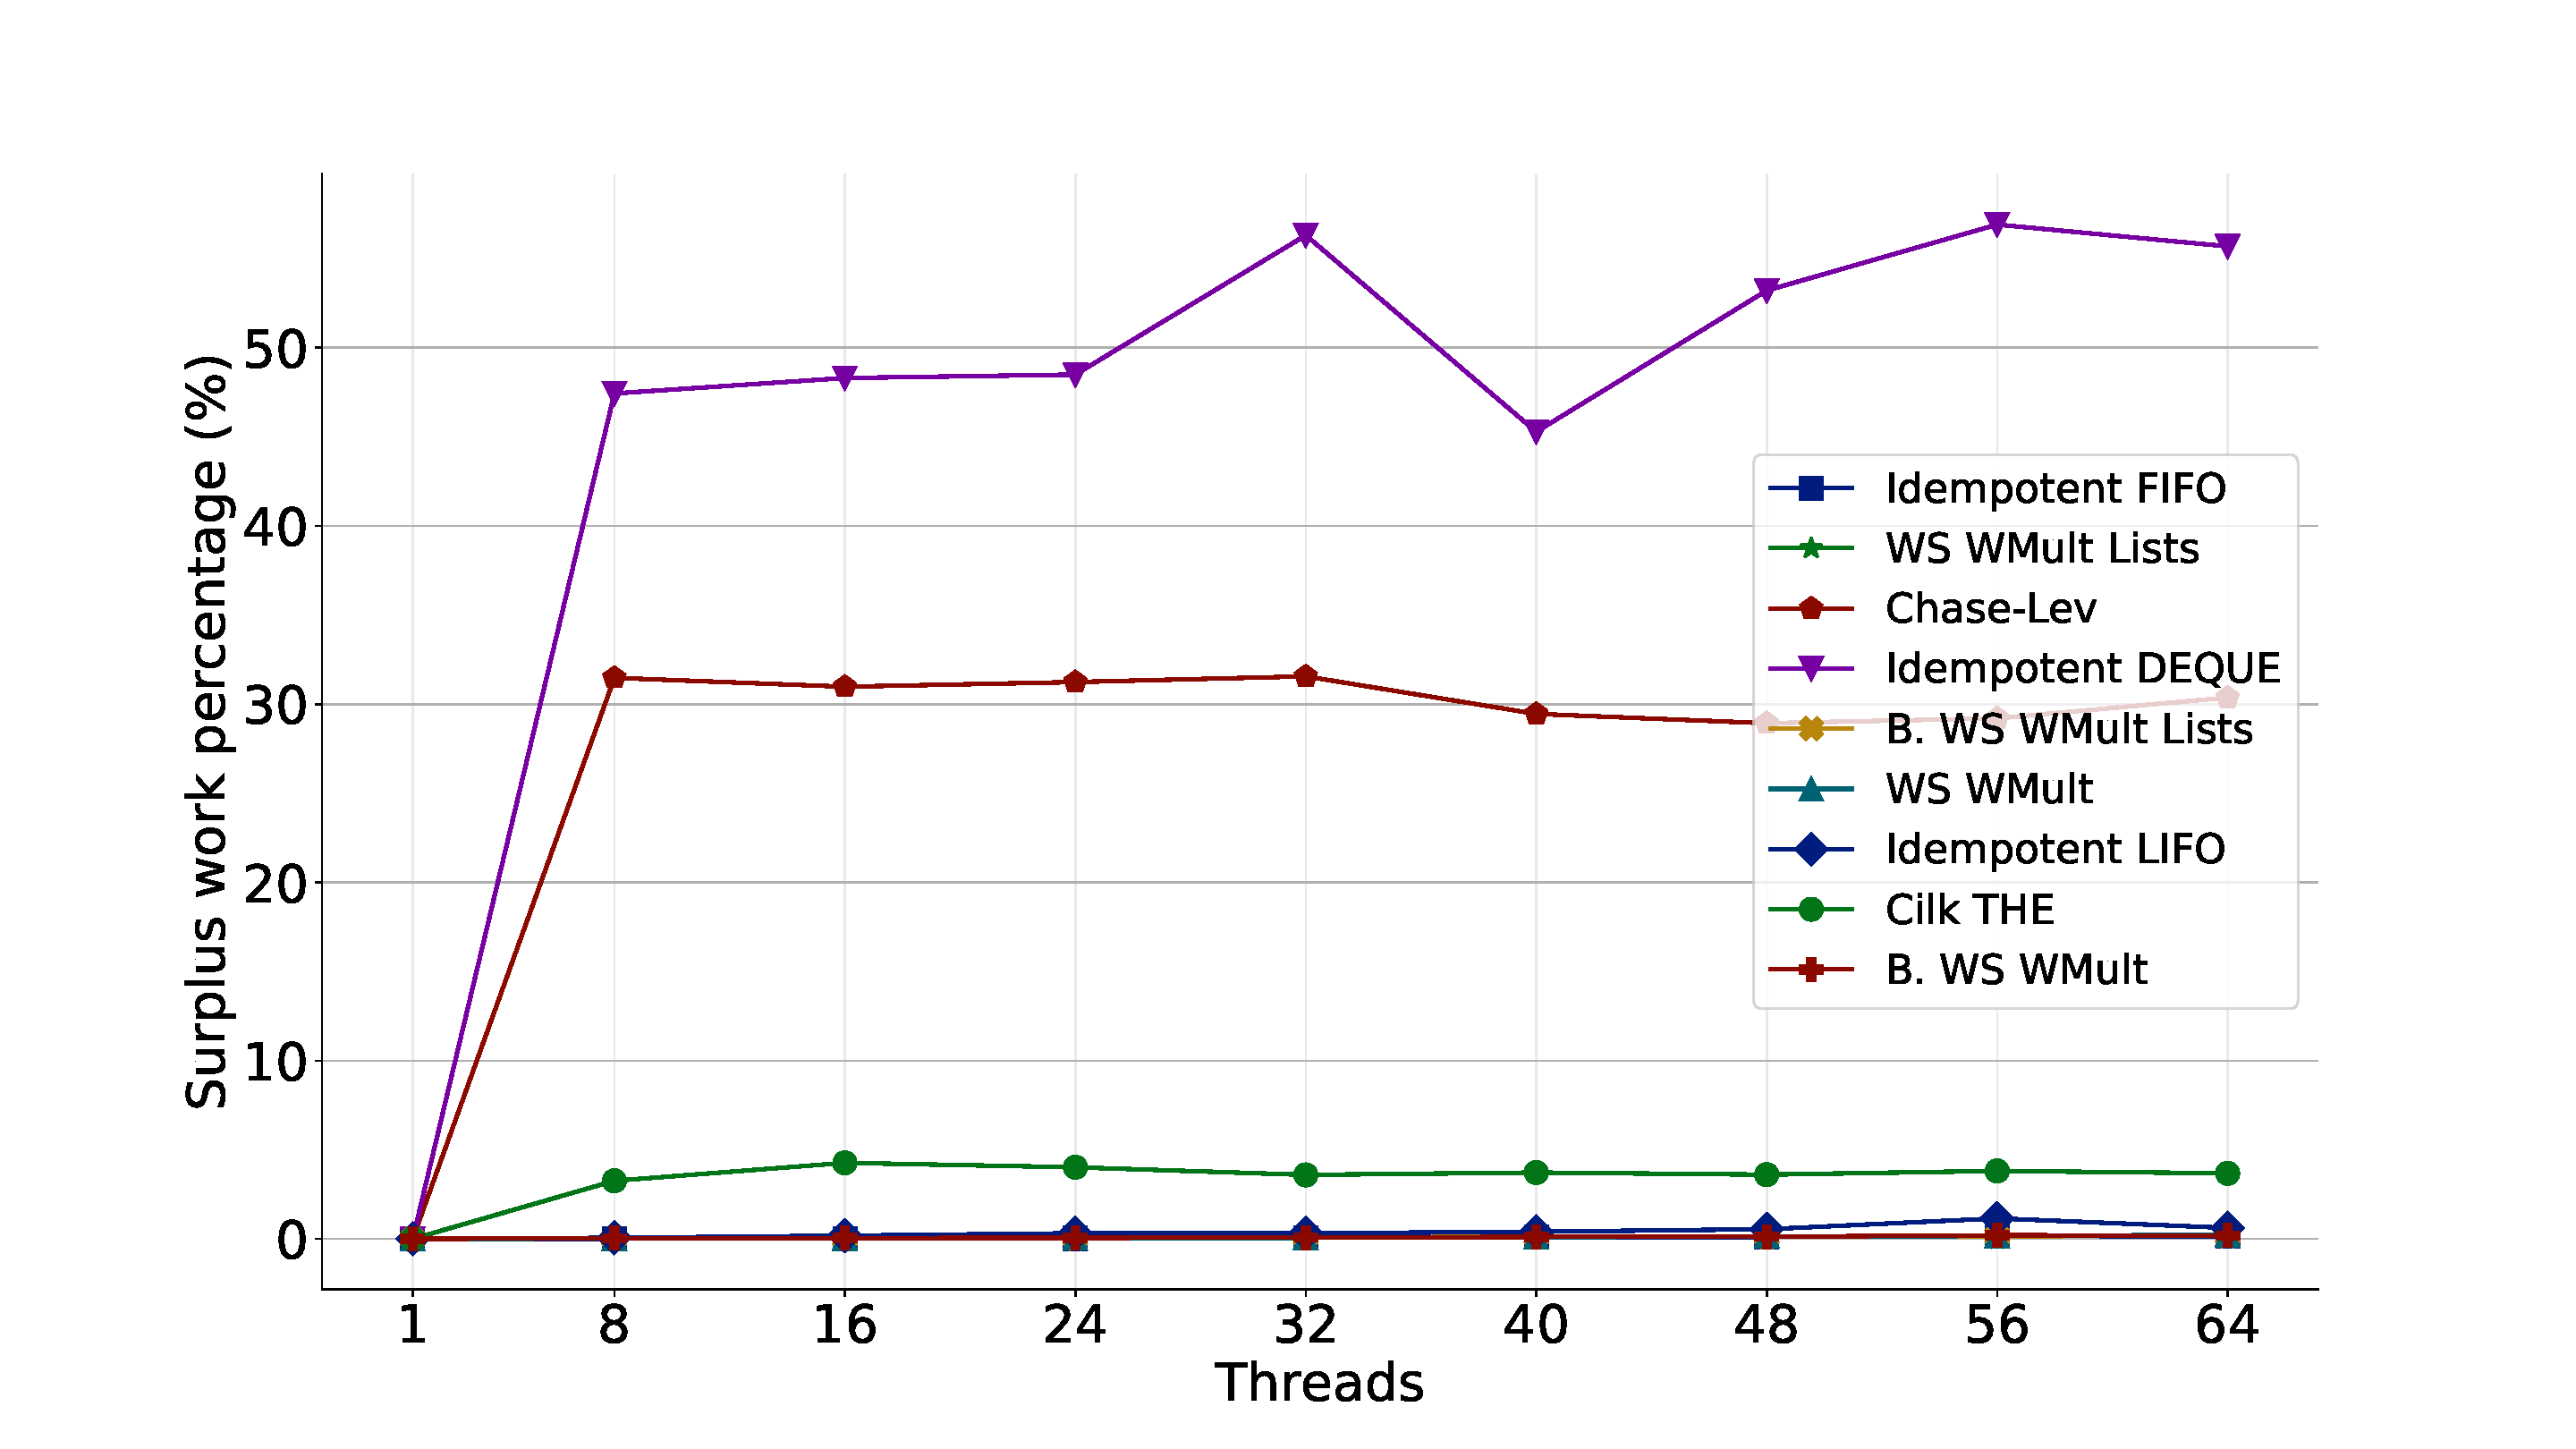
\includegraphics[width=0.48\textwidth]{contents/backmatter/evaluation/mult-torus_2d_directed_256.pdf}
  }
  \subfloat[\label{fig:surplustorus2ddirected-appx:1000000}Surplus work: Directed Torus 2D. Initial size of 1,000,000 items]{
    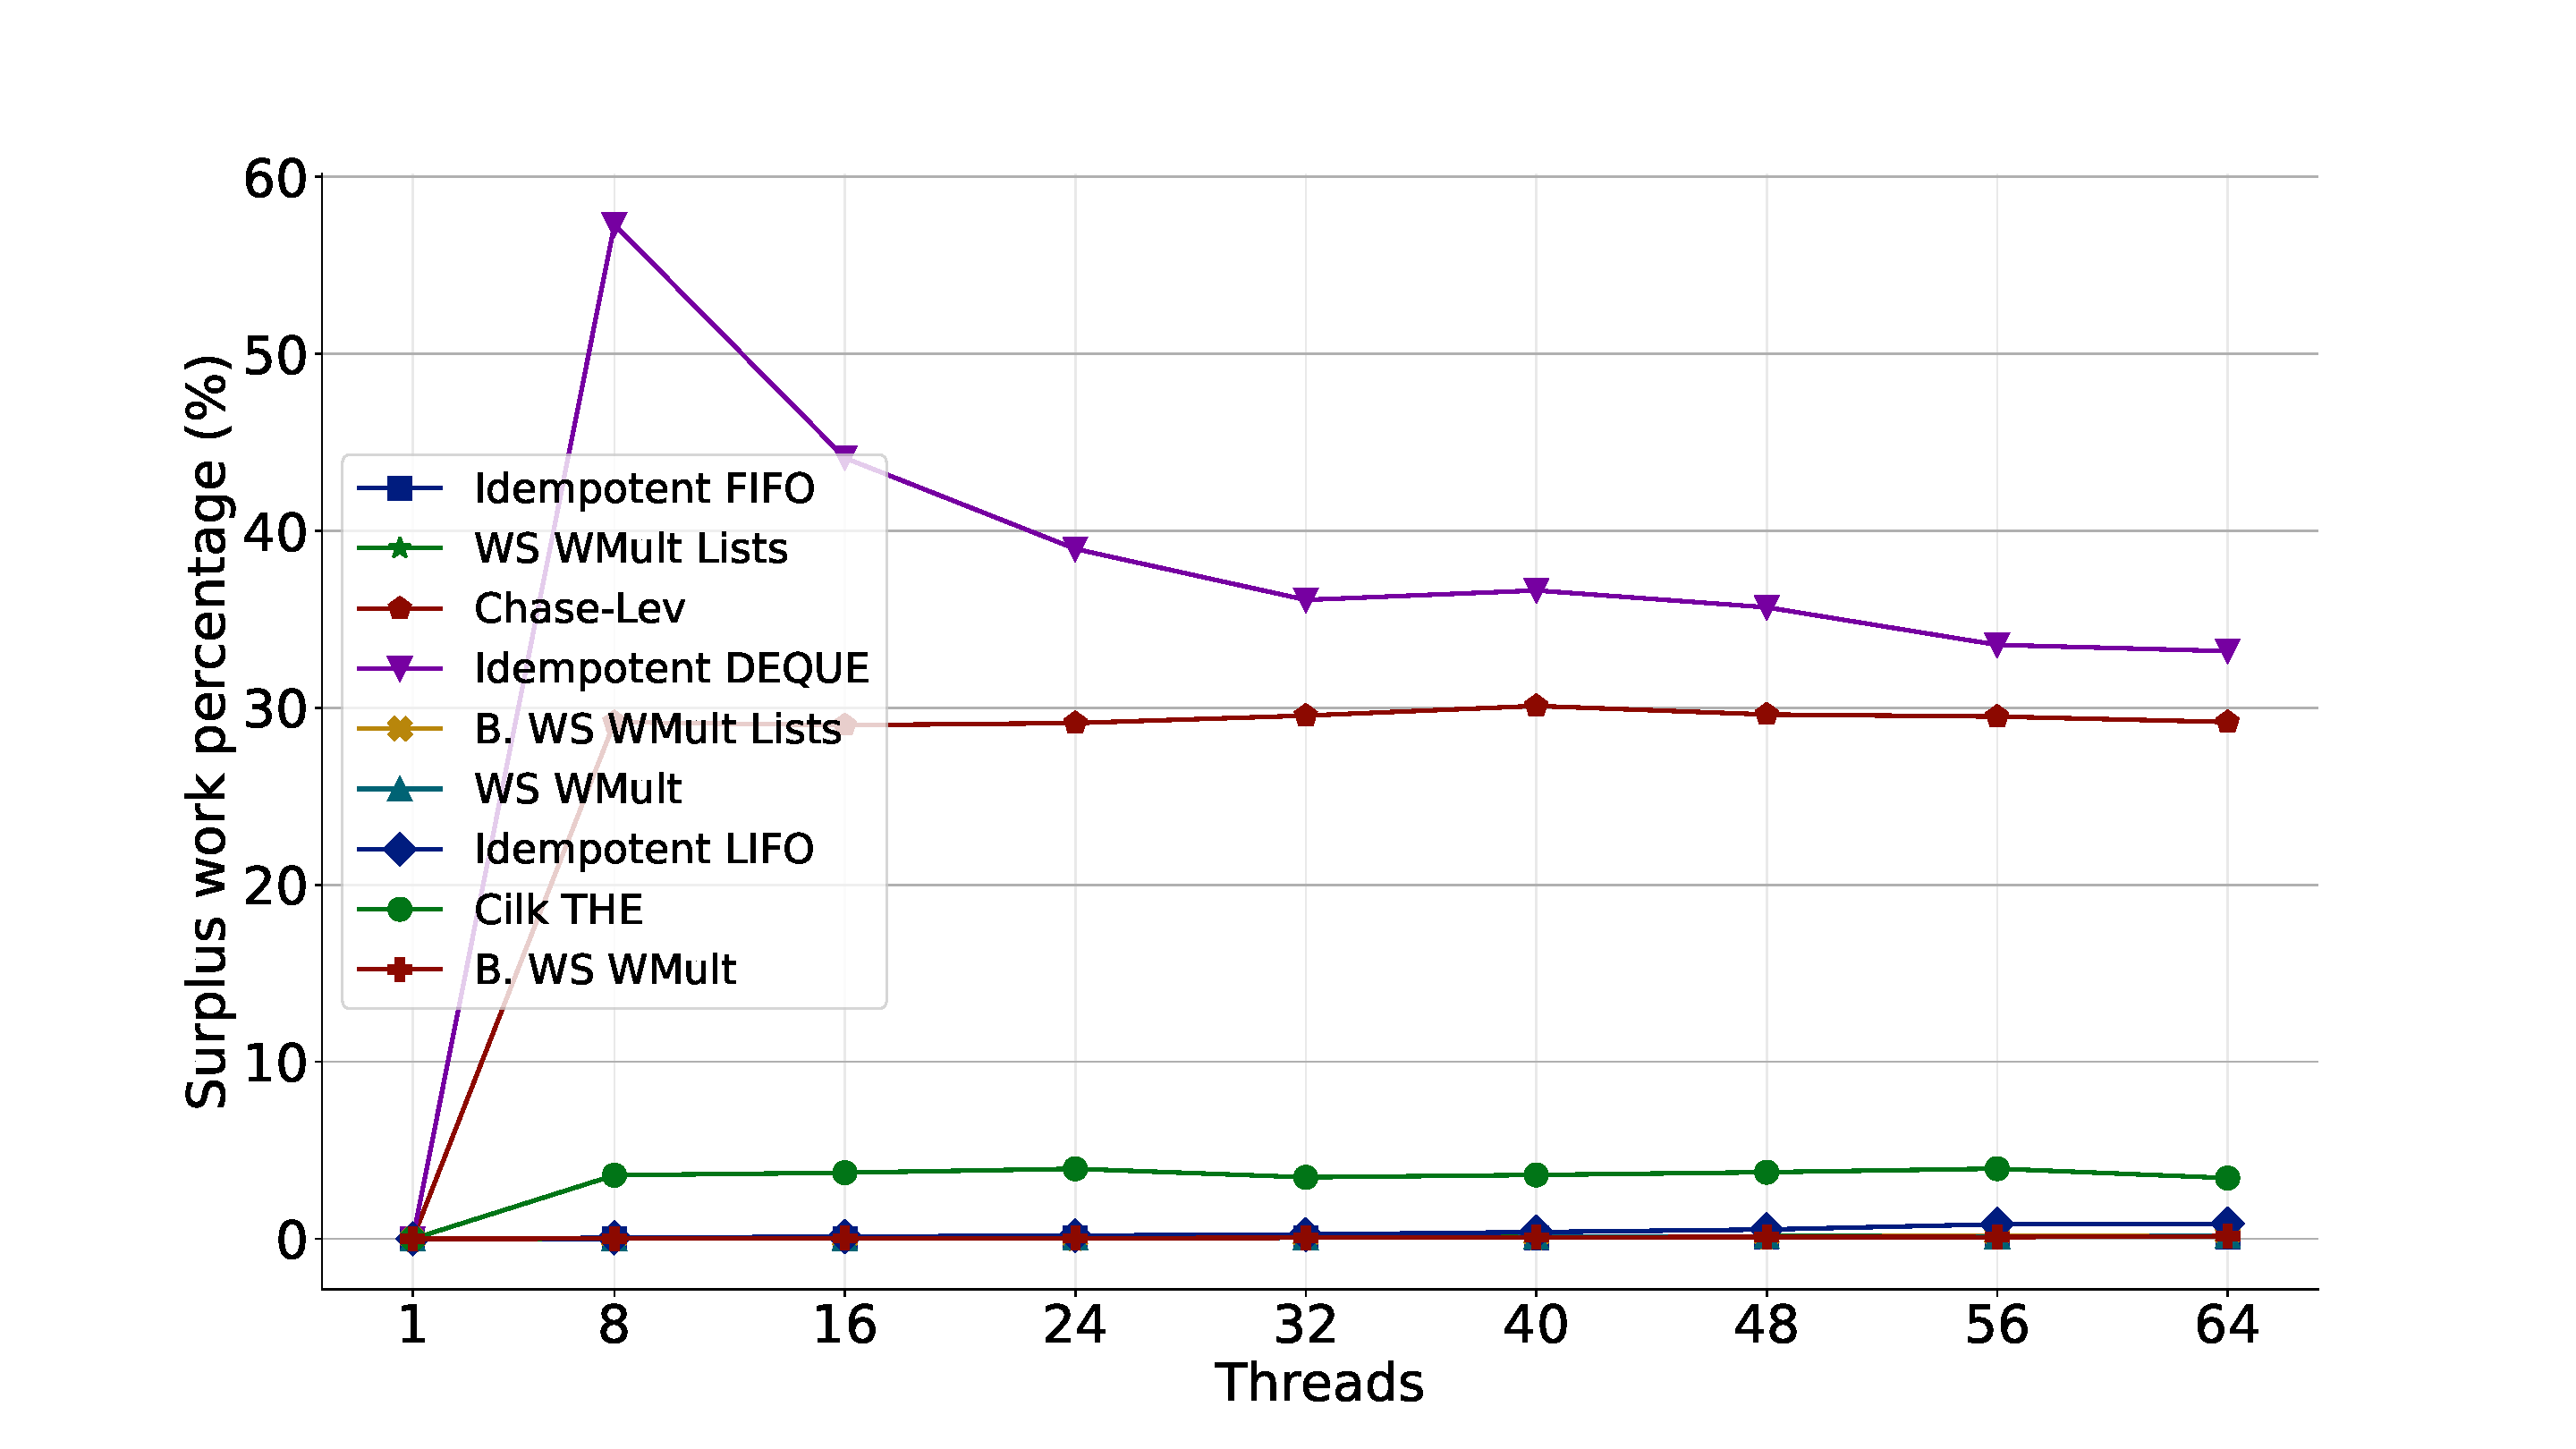
\includegraphics[width=0.48\textwidth]{contents/backmatter/evaluation/mult-torus_2d_directed_1m.pdf}
  }

  \subfloat[\label{fig:surplustorus2dundirected-appx:256}Surplus work: Undirected Torus 2D. Initial size of 256 items]{
    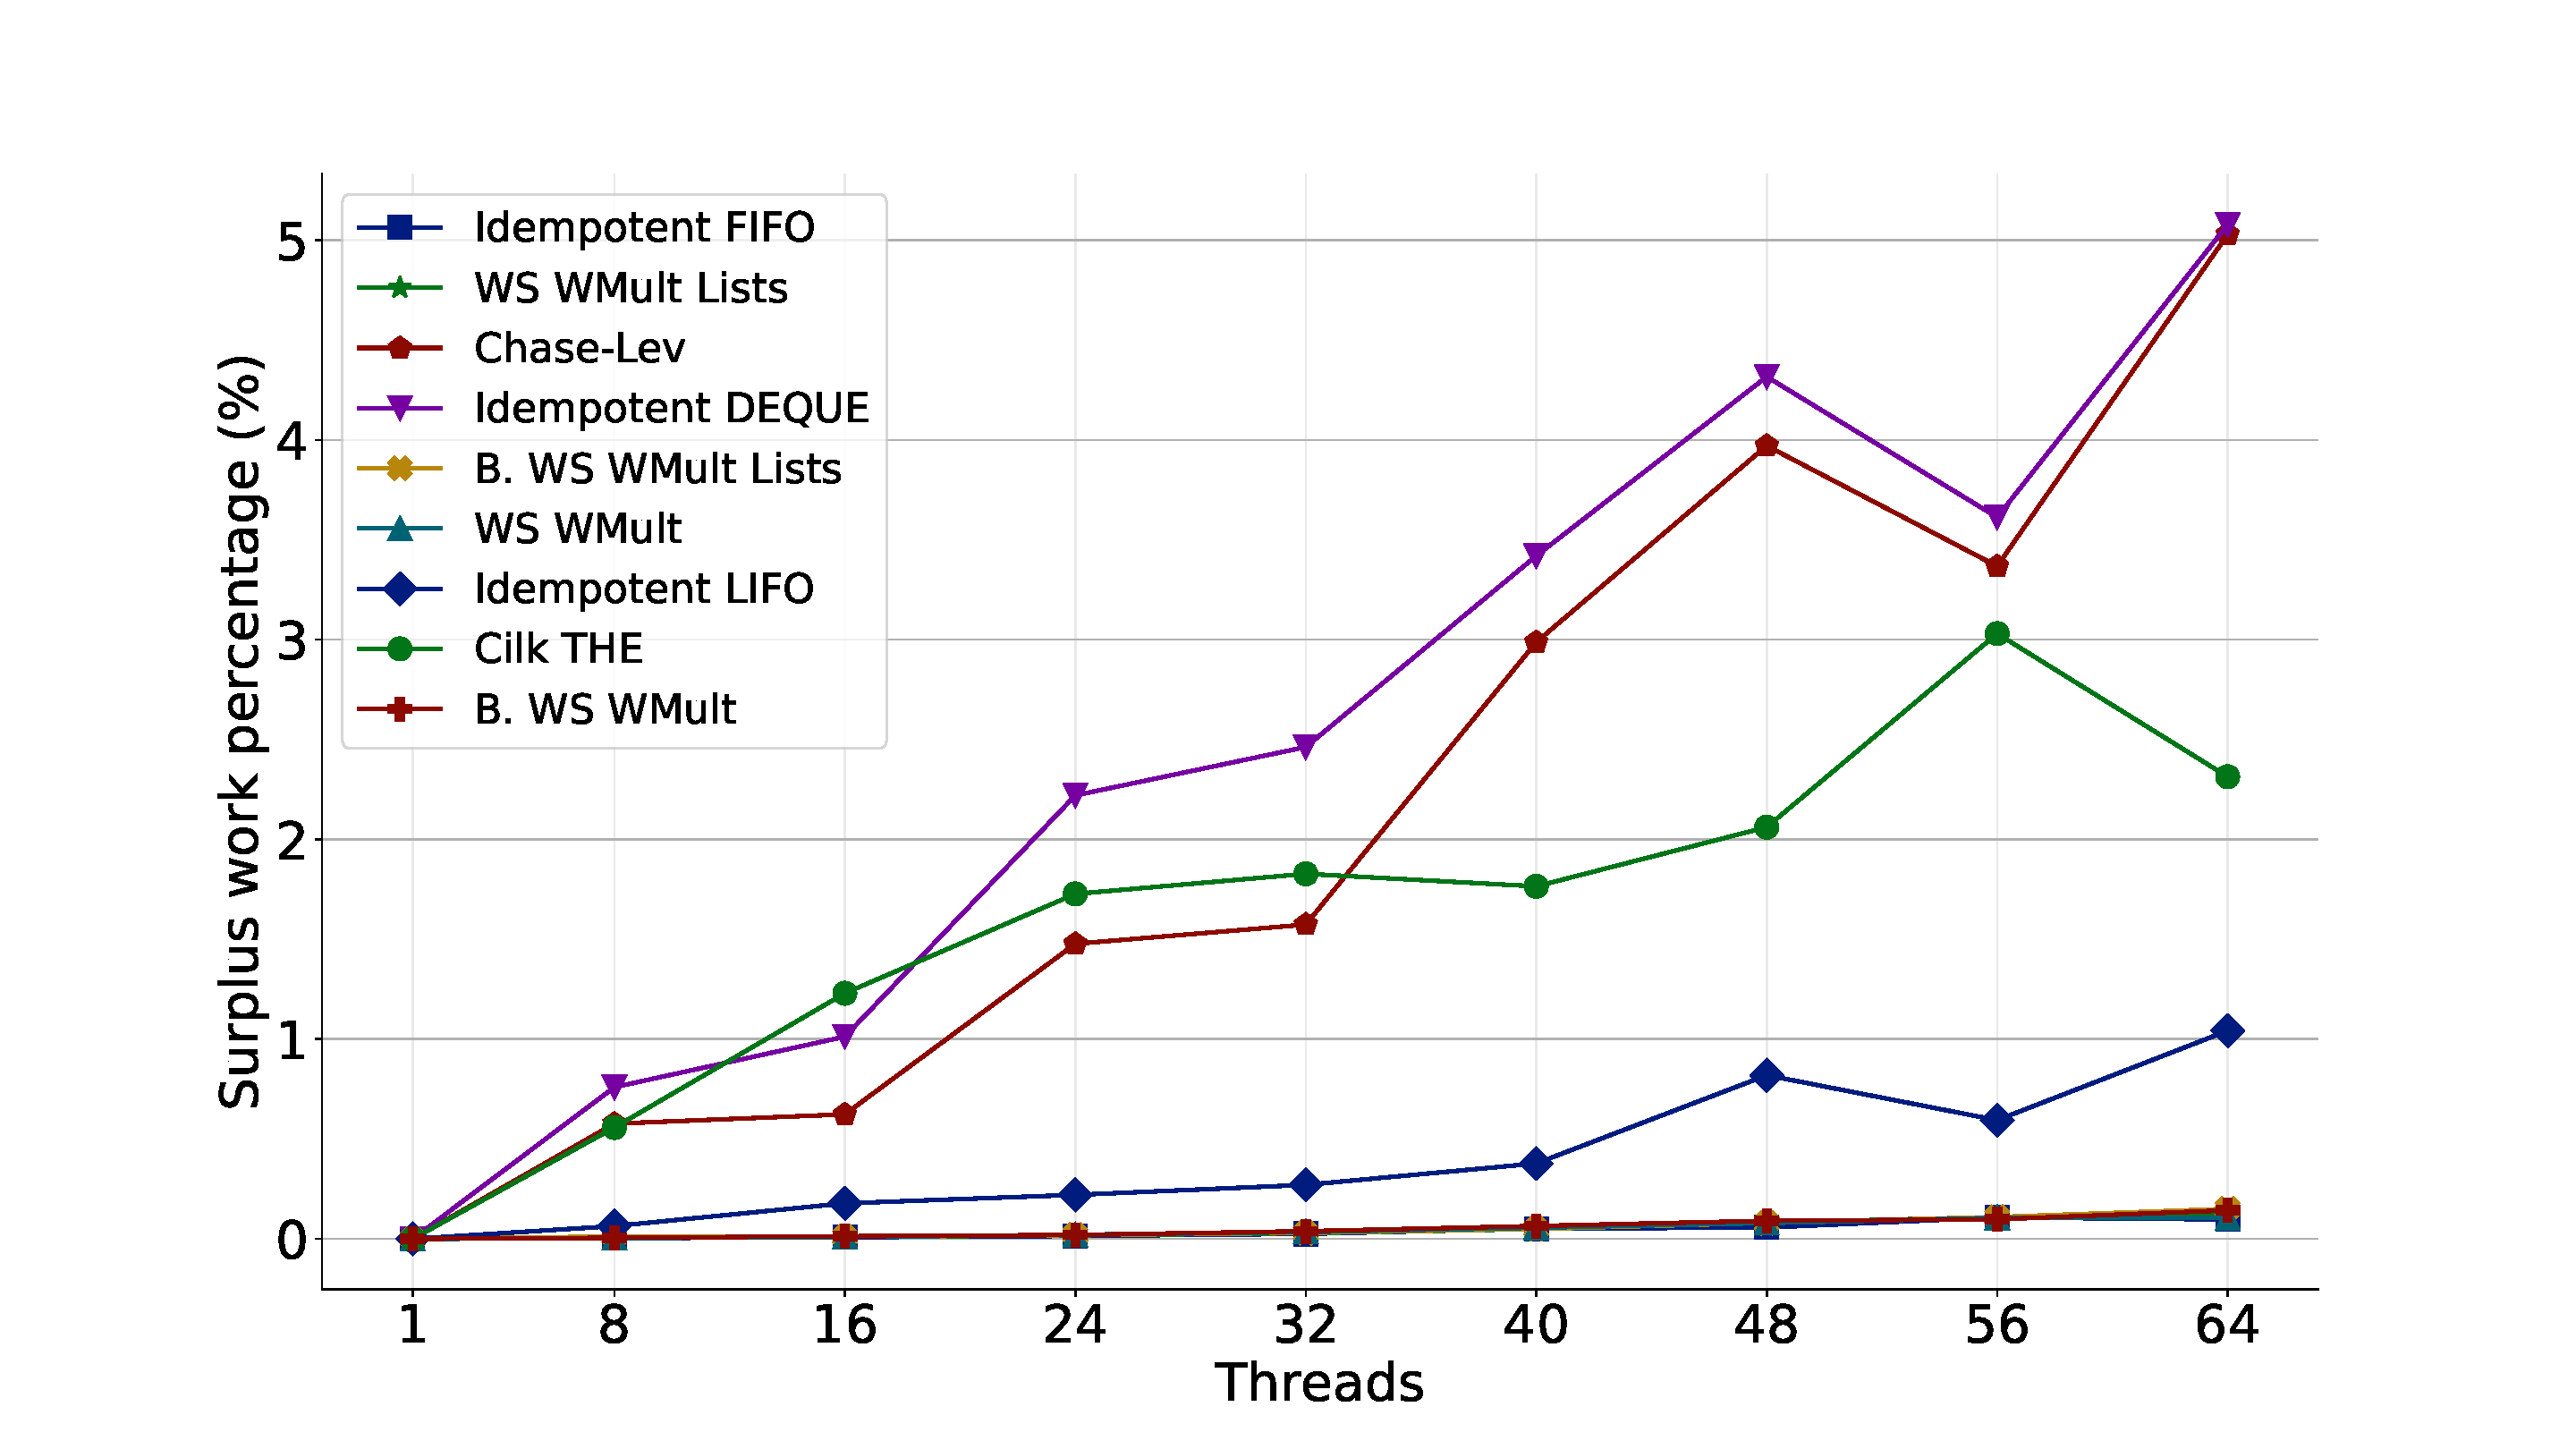
\includegraphics[width=0.48\textwidth]{contents/backmatter/evaluation/mult-torus_2d_undirected_256.pdf}
  }
  \subfloat[\label{fig:surplustorus2dundirected:1000000}Surplus work: Undirected Torus 2D. Initial size of 1,000,000 items]{
    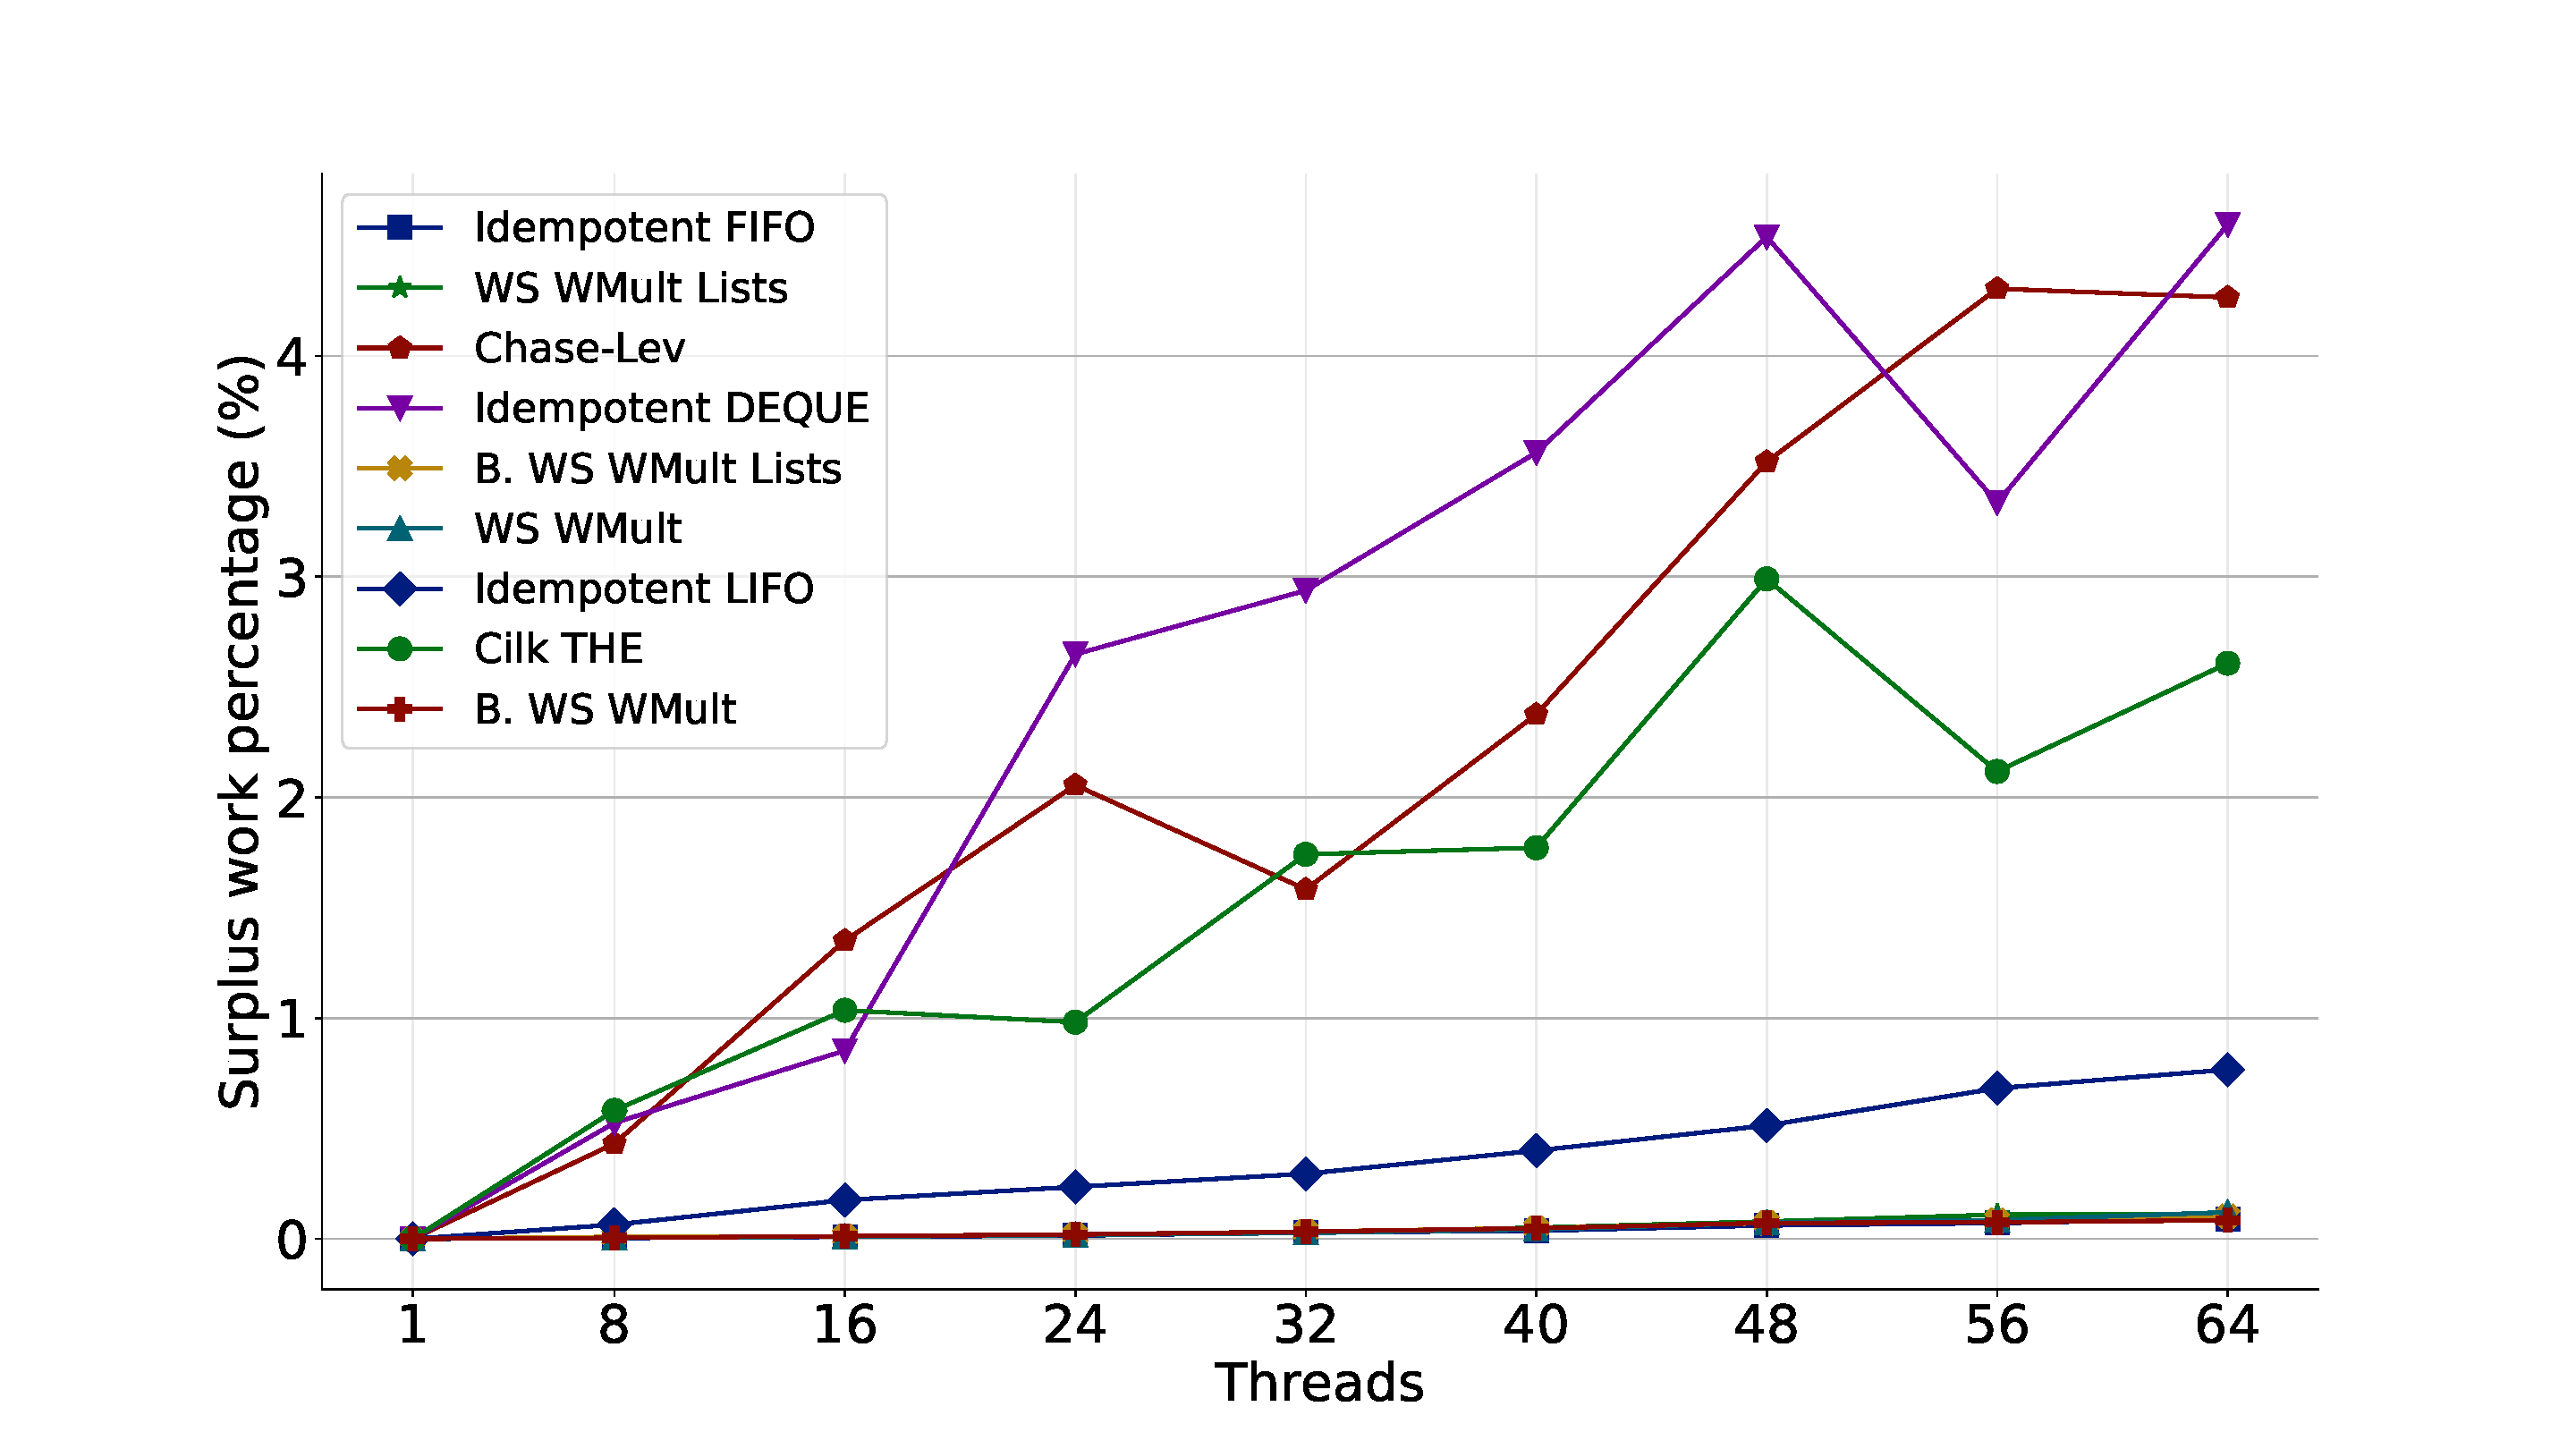
\includegraphics[width=0.48\textwidth]{contents/backmatter/evaluation/mult-torus_2d_undirected_1m.pdf}
  }

  \caption{\label{fig:surplusgraphapplicationtorus2d} Surplus work
    (percentage) of the experiments.  Surplus work: the difference between
    the total number of \Puts and the number of puts in sequential executions
    (i.e., $1,000,000$).}
\end{figure}

\begin{figure}[!ht]
  \subfloat[\label{fig:exec-surplustorus2ddirected-appx:256}Executed surplus work: Directed Torus 2D. Initial size of 256 items]{
    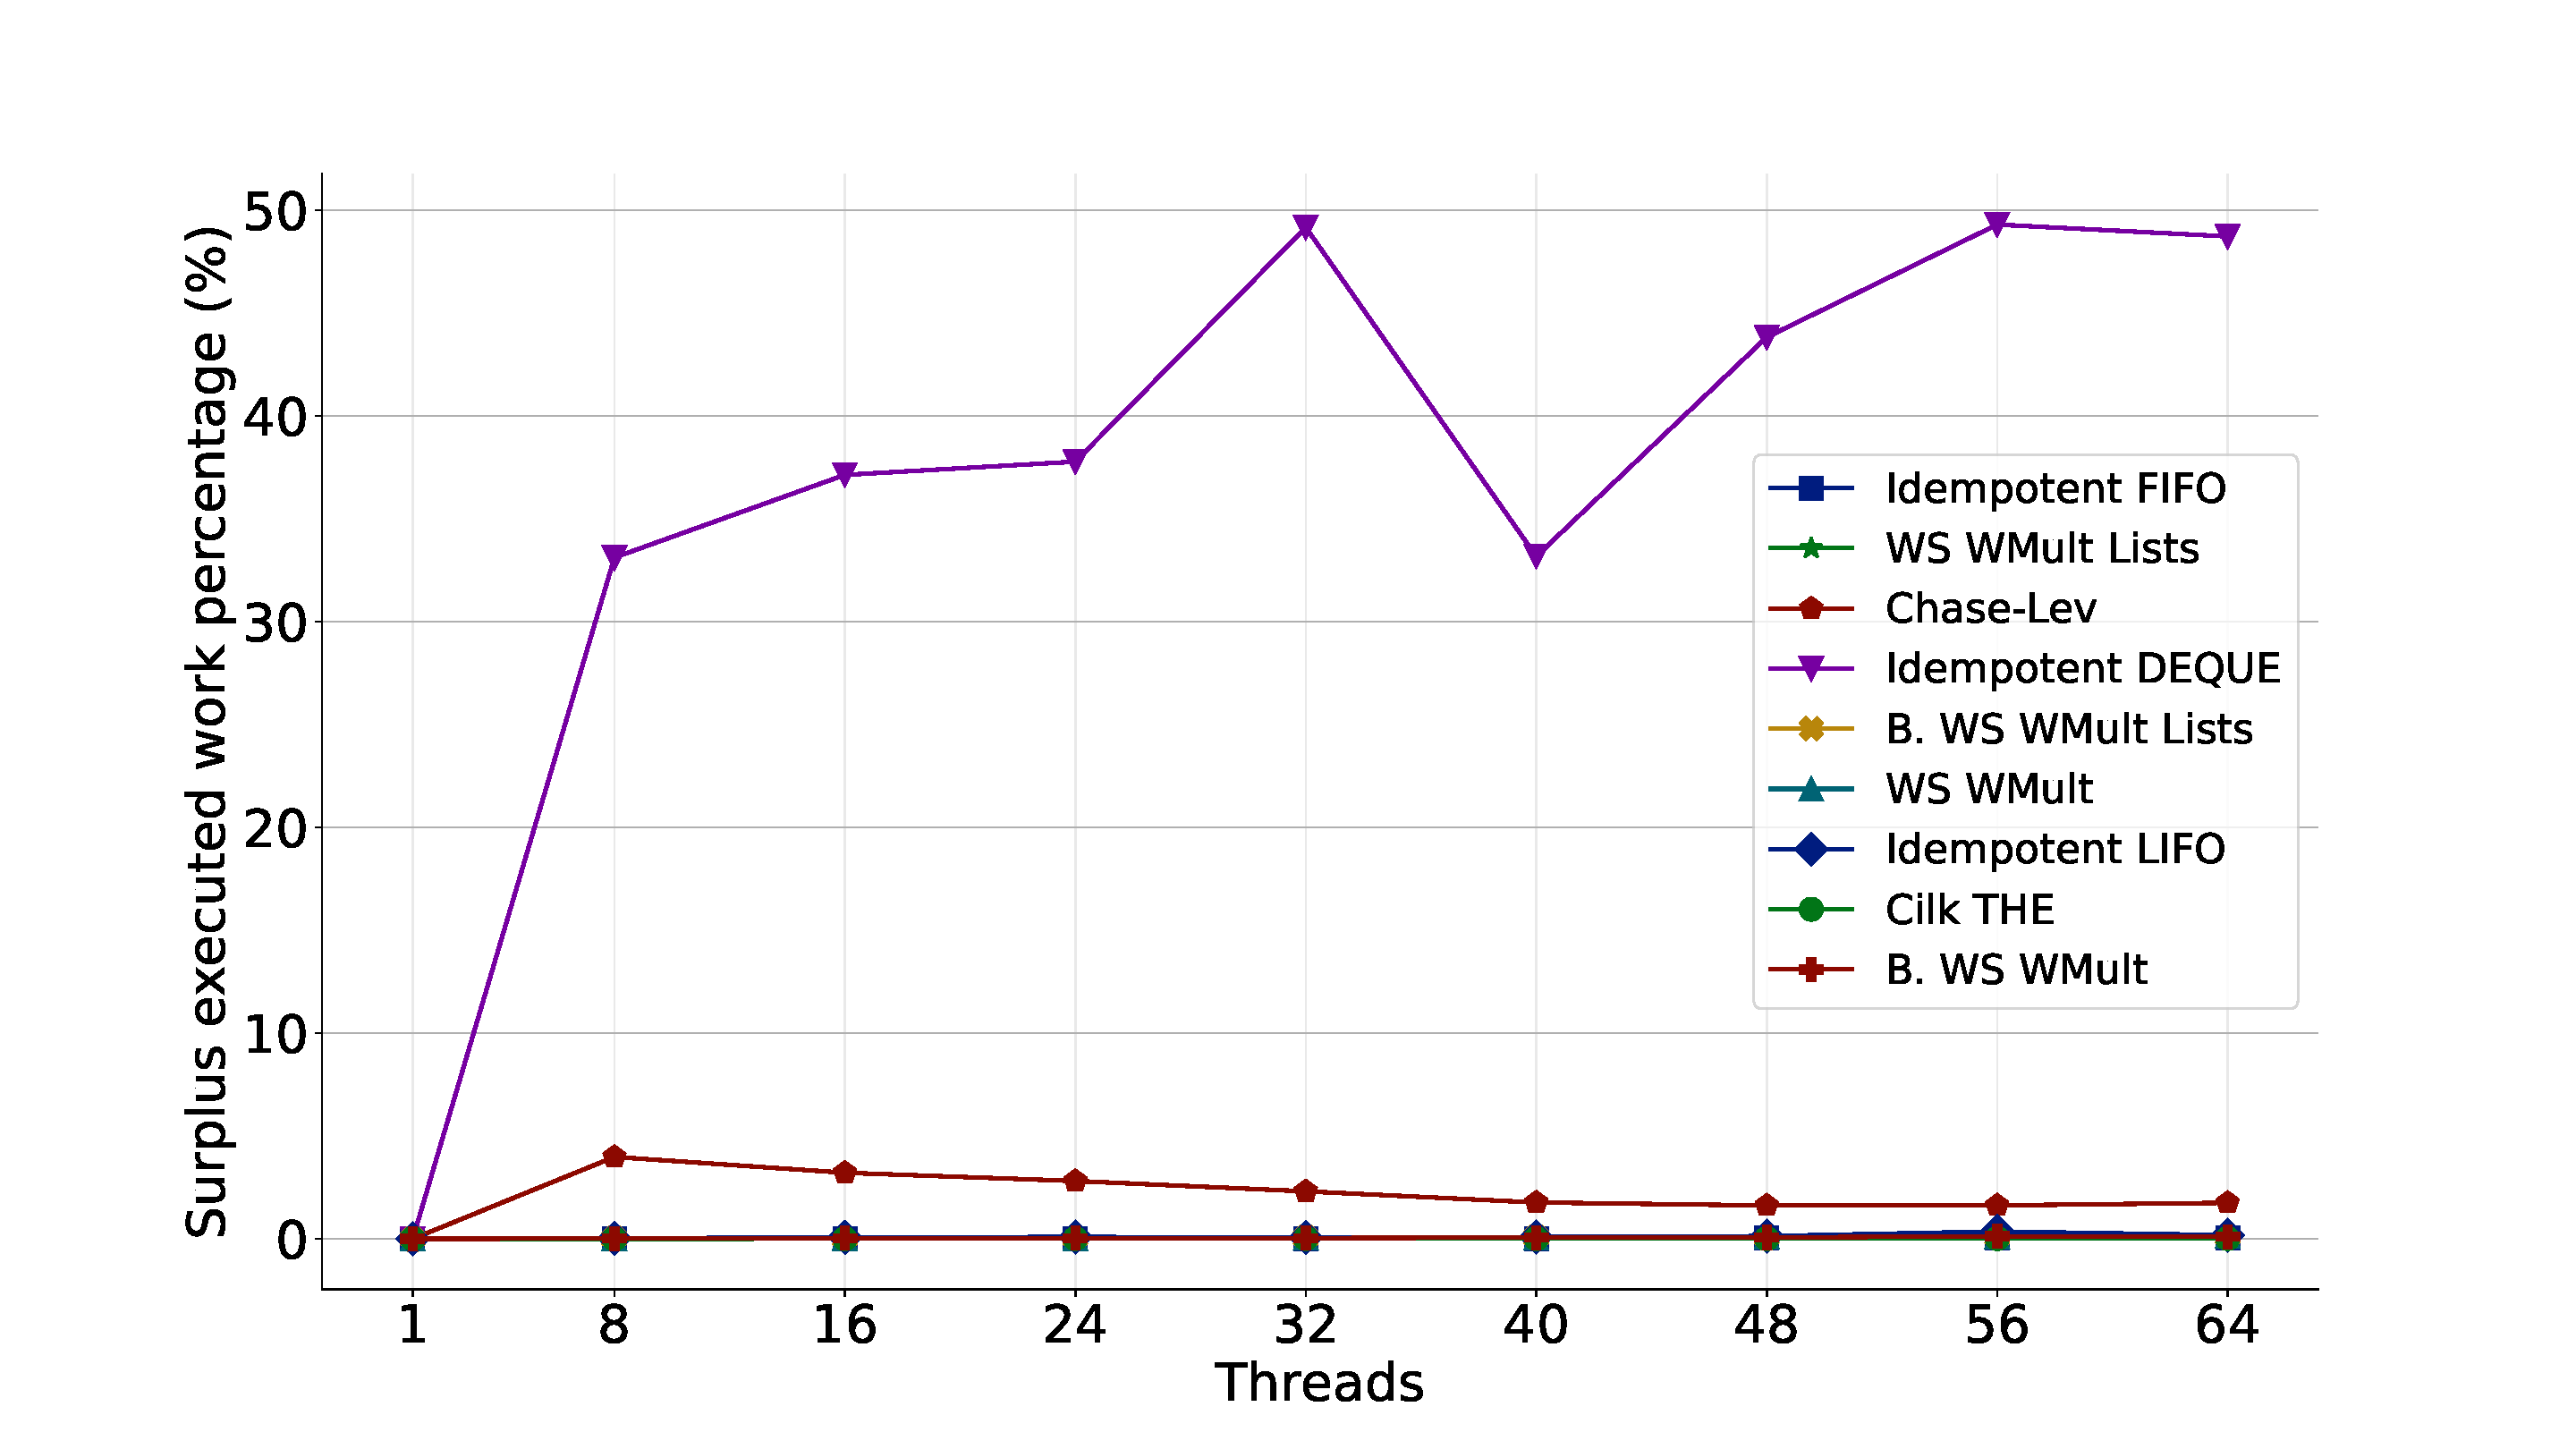
\includegraphics[width=0.48\textwidth]{contents/backmatter/evaluation/mult-exec-torus_2d_directed_256.pdf}
  }
  \subfloat[\label{fig:exec-surplustorus2ddirected-appx:1000000}Executed
  surplus work: Directed Torus 2D. Initial size of 1,000,000 items]{
    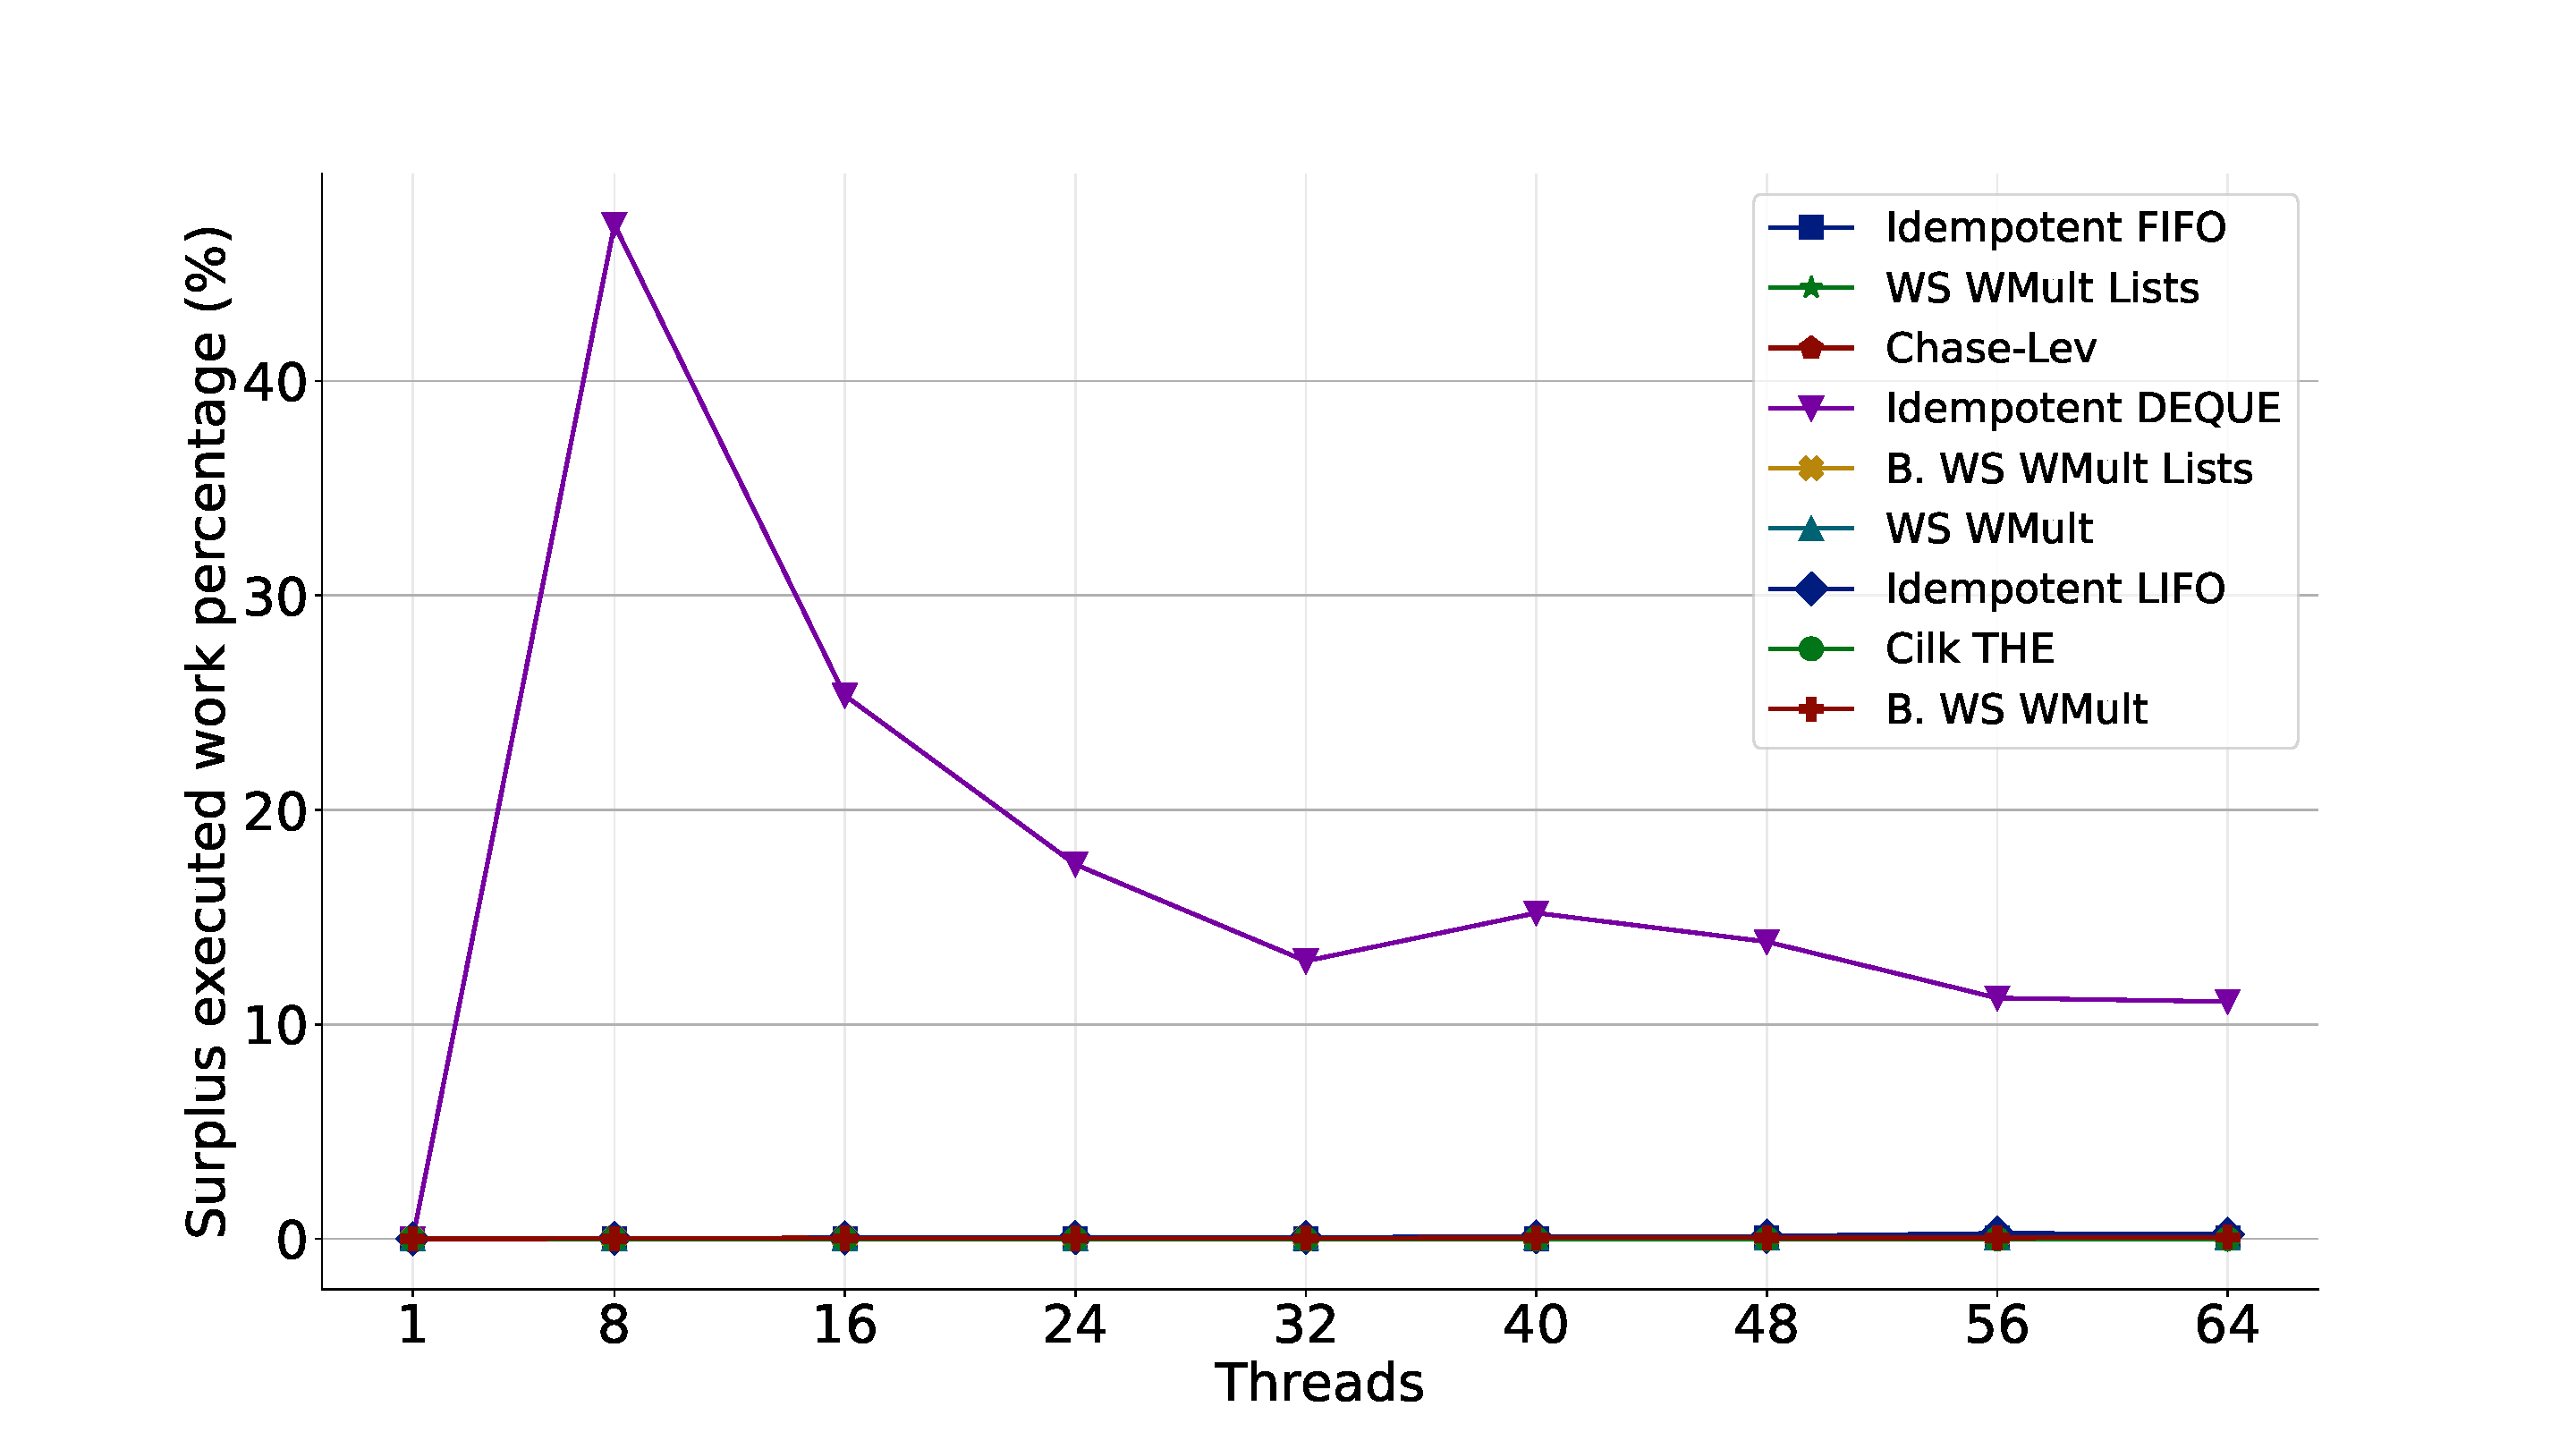
\includegraphics[width=0.48\textwidth]{contents/backmatter/evaluation/mult-exec-torus_2d_directed_1m.pdf}
  }

  \subfloat[\label{fig:exec-surplustorus2dundirected-appx:256}Executed
  surplus work: Undirected Torus 2D. Initial size of 256 items]{
    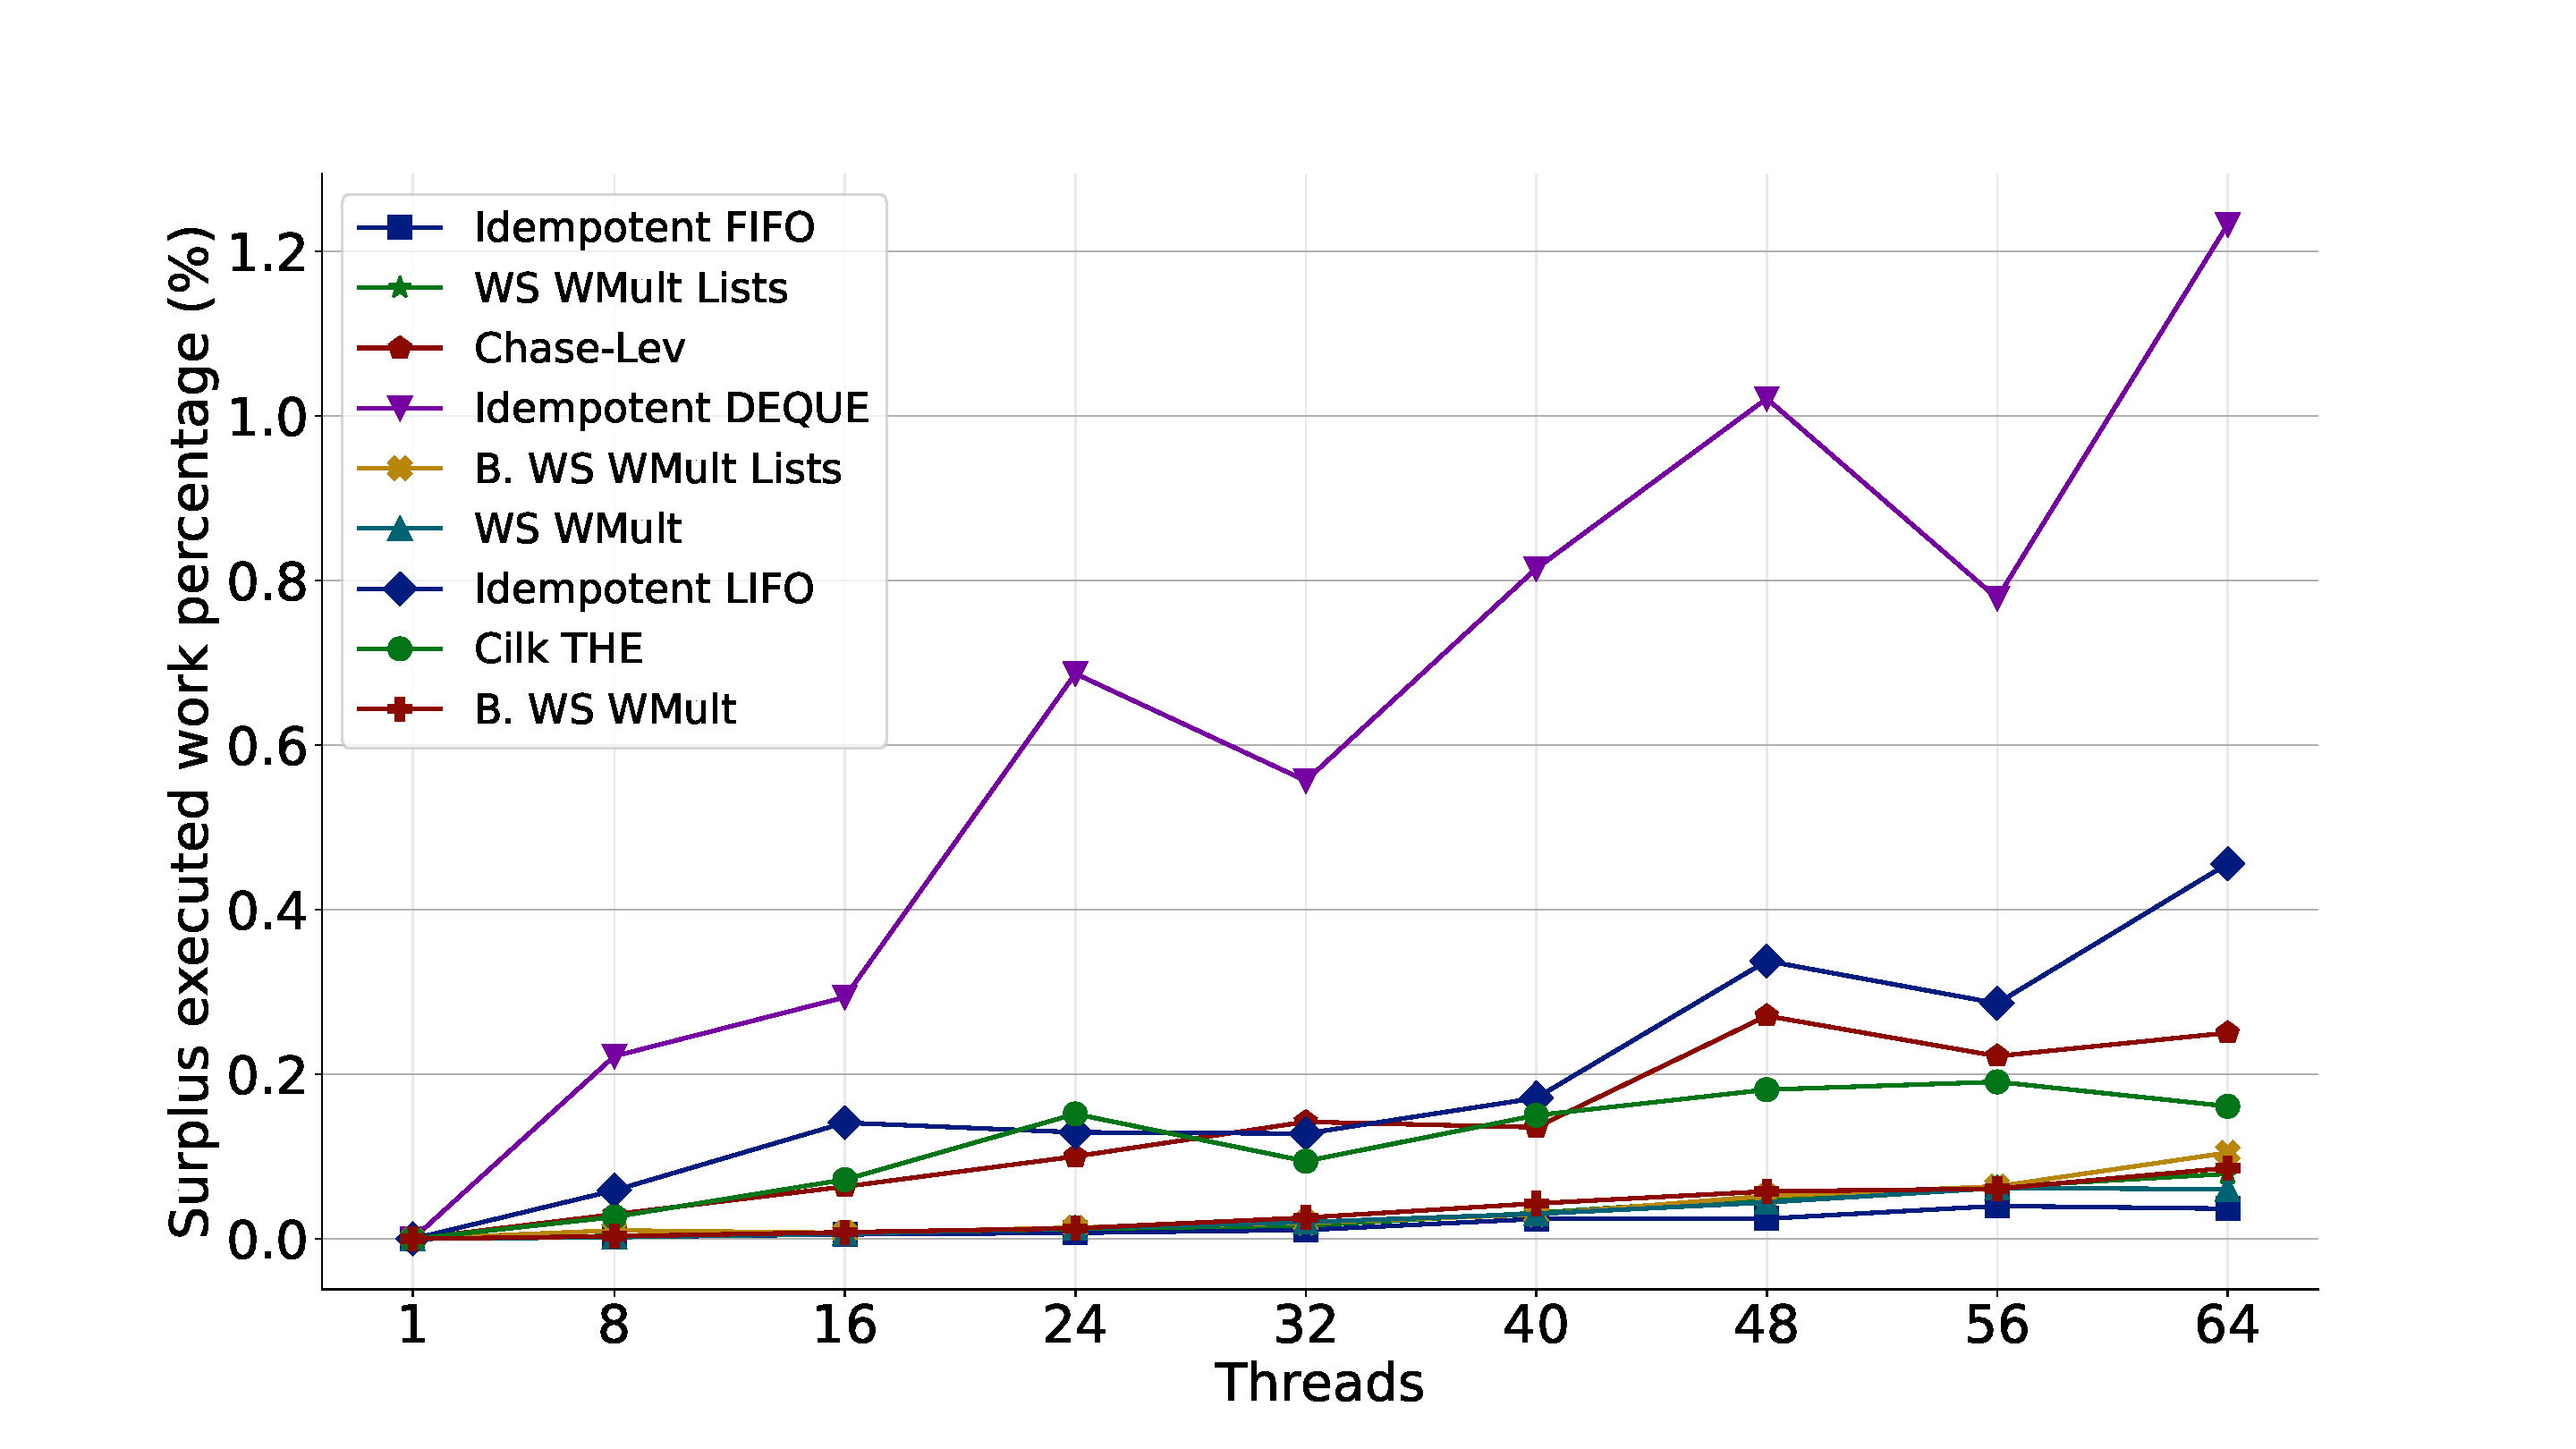
\includegraphics[width=0.48\textwidth]{contents/backmatter/evaluation/mult-exec-torus_2d_undirected_256.pdf}
  }
  \subfloat[\label{fig:exec-surplustorus2dundirected:1000000}Executed surplus work: Undirected Torus 2D. Initial size of 1,000,000 items]{
    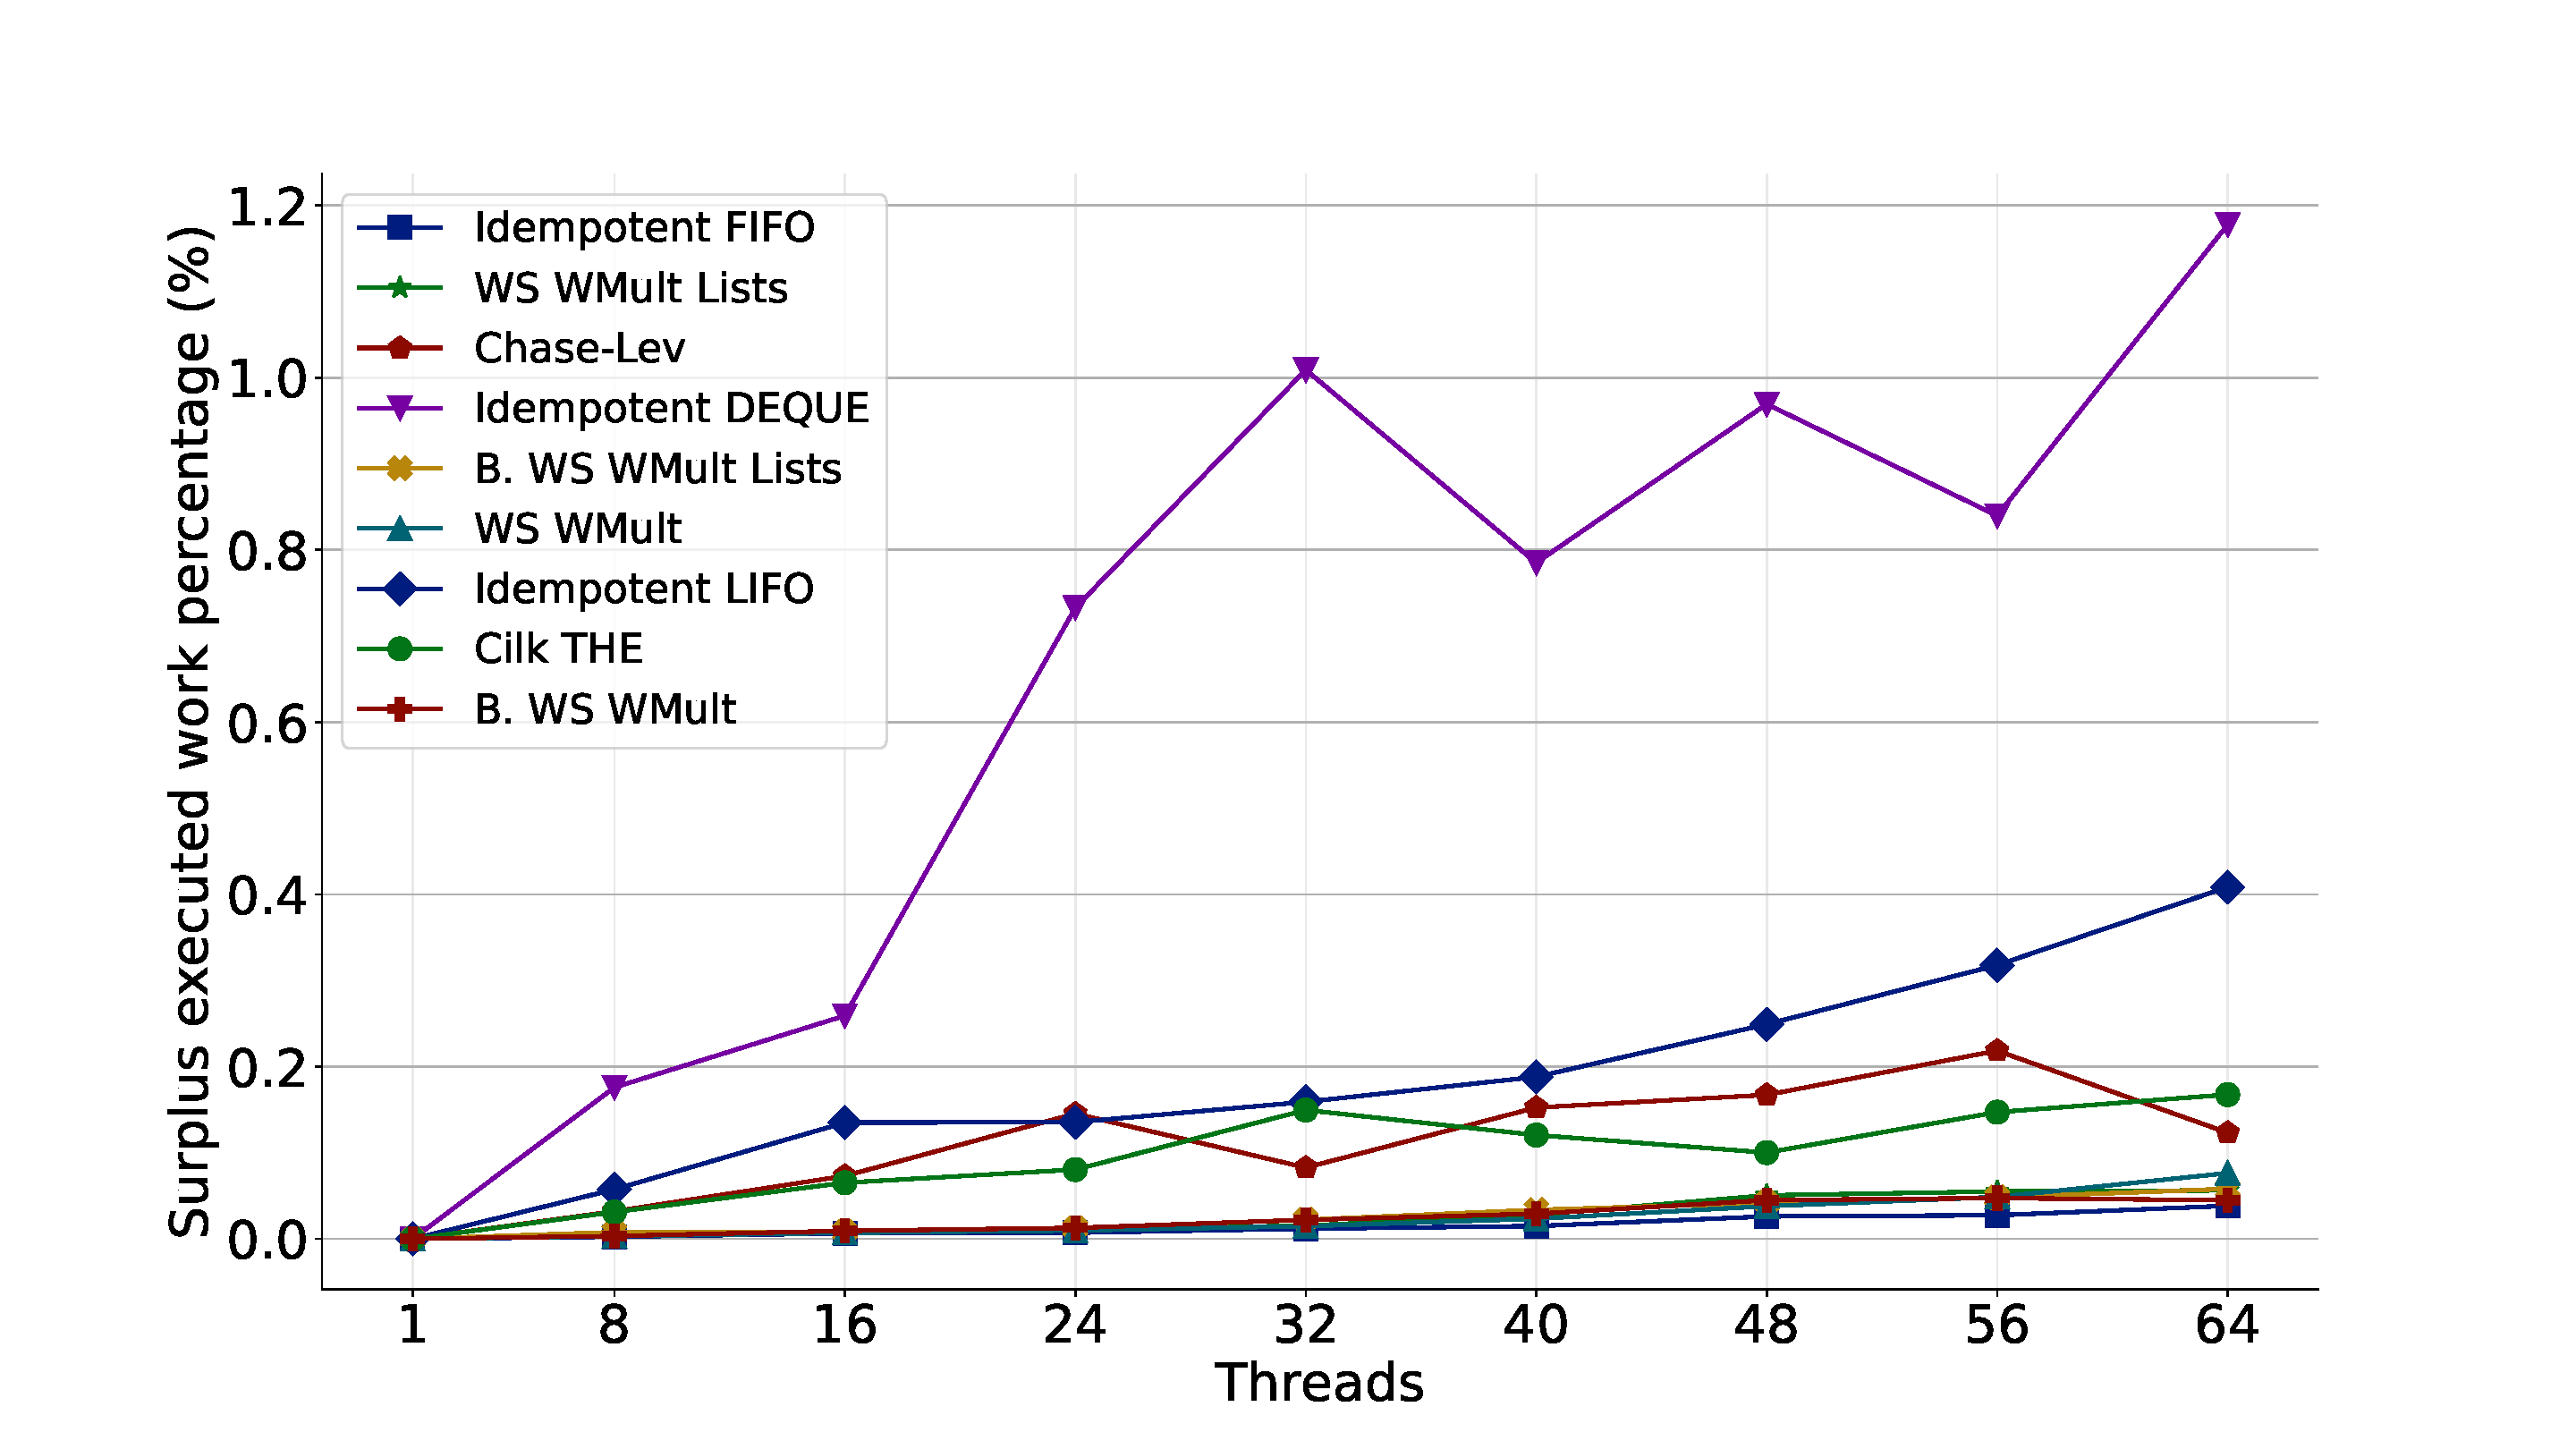
\includegraphics[width=0.48\textwidth]{contents/backmatter/evaluation/mult-exec-torus_2d_undirected_1m.pdf}
  }

  \caption{\label{fig:exec-surplusgraphapplicationtorus2d-appendix}
    Executed surplus work (percentage) of the experiments.  Surplus
    work: the difference between the total number of \Takes and the
    number of takes in sequential executions (i.e., $1,000,000$).}
\end{figure}

\clearpage
\subsubsection{Directed Torus 2D 60\%. Initial size of 256 items.}
\begin{table}[!ht]
\centering
\resizebox{\textwidth}{!}{\begin{tabular}{lrrrrrrrrrrrrrrr}
\toprule
\textbf{Algorithm} & \multicolumn{5}{l}{Chase-Lev} & \multicolumn{5}{l}{Cilk THE} & \multicolumn{5}{l}{Idempotent LIFO} \\
\textbf{Operation} &       Puts &      Takes & Difference (\%) & Surplus (\%) & Executed Surplus (\%) &       Puts &      Takes & Difference (\%) & Surplus (\%) & Executed Surplus (\%) &            Puts &      Takes & Difference (\%) & Surplus (\%) & Executed Surplus (\%) \\
\textbf{Processes} & \multicolumn{4}{l}{} & \multicolumn{4}{l}{} & \multicolumn{4}{l}{}\\ \midrule
\textbf{1 } & 1000000.00 & 1000000.00 &           0.00 &        0.00 &                 0.00 & 1000000.00 & 1000000.00 &           0.00 &        0.00 &                 0.00 &      1000000.00 & 1000000.00 &           0.00 &        0.00 &                 0.00 \\
\textbf{8 } & 1020806.00 & 1000143.60 &           2.02 &        2.04 &                 0.01 & 1023550.20 & 1000084.60 &           2.29 &        2.30 &                 0.01 &      1027143.60 & 1008311.80 &           1.83 &        2.64 &                 0.82 \\
\textbf{16} & 1037467.40 & 1000165.40 &           3.60 &        3.61 &                 0.02 & 1042807.00 & 1000167.00 &           4.09 &        4.10 &                 0.02 &      1050478.40 & 1012666.40 &           3.60 &        4.81 &                 1.25 \\
\textbf{24} & 1064950.60 & 1000357.80 &           6.07 &        6.10 &                 0.04 & 1050968.80 & 1000198.80 &           4.83 &        4.85 &                 0.02 &      1060968.00 & 1010891.40 &           4.72 &        5.75 &                 1.08 \\
\textbf{28} & 1068789.20 & 1000359.00 &           6.40 &        6.44 &                 0.04 & 1059995.60 & 1000244.20 &           5.64 &        5.66 &                 0.02 &      1073664.80 & 1010931.40 &           5.84 &        6.86 &                 1.08 \\
\textbf{32} & 1073080.40 & 1000402.40 &           6.77 &        6.81 &                 0.04 & 1073922.60 & 1000298.60 &           6.86 &        6.88 &                 0.03 &      1069279.20 & 1015430.60 &           5.04 &        6.48 &                 1.52 \\
\textbf{40} & 1097050.60 & 1000536.00 &           8.80 &        8.85 &                 0.05 & 1060958.00 & 1000283.80 &           5.72 &        5.75 &                 0.03 &      1092589.80 & 1012147.40 &           7.36 &        8.47 &                 1.20 \\
\textbf{48} & 1117179.80 & 1000760.00 &          10.42 &       10.49 &                 0.08 & 1079921.60 & 1000413.00 &           7.36 &        7.40 &                 0.04 &      1105993.60 & 1014937.40 &           8.23 &        9.58 &                 1.47 \\
\textbf{56} & 1119717.40 & 1000970.80 &          10.61 &       10.69 &                 0.10 & 1070216.20 & 1000368.00 &           6.53 &        6.56 &                 0.04 &      1100948.60 & 1014673.40 &           7.84 &        9.17 &                 1.45 \\
\textbf{64} & 1117871.00 & 1000870.80 &          10.47 &       10.54 &                 0.09 & 1077195.00 & 1000351.00 &           7.13 &        7.17 &                 0.04 &      1098635.00 & 1013103.20 &           7.79 &        8.98 &                 1.29 \\
\bottomrule
\end{tabular}}
\label{difference-Torus_2D_60_directed-256-CHASELEV-CILK-IDEMPOTENT_LIFO}
\caption{The number of puts and takes performed during the
    spanning tree experiment on a Torus 2D 60 directed graph with an initial size
    of 256 items is provided. The table presents data on the
    following algorithms: Chase-Lev, Cilk THE, and
    Idempotent LIFO. Furthermore, we present the percentage difference
    between the number of puts and takes for each available thread,
    relative to the total number of puts. Finally, also we show the
    "surplus" work, which is the difference of the total number of
    \Puts (Work to be scheduled) and the total number of \Puts in
    sequential executions (i.e., 1,000,000), and the "executed surplus
    work", which is the difference between the total number of \Takes
    (actual work executed) and the total of \Takes in sequential
    executions.}
\end{table}

\begin{table}[!ht]
\centering
\resizebox{\textwidth}{!}{\begin{tabular}{lrrrrrrrrrrrrrrr}
\toprule
\textbf{Algorithm} & \multicolumn{5}{l}{Idempotent DEQUE} & \multicolumn{5}{l}{Idempotent FIFO} & \multicolumn{5}{l}{WS WMult} \\
\textbf{Operation} &             Puts &      Takes & Difference (\%) & Surplus (\%) & Executed Surplus (\%) &            Puts &      Takes & Difference (\%) & Surplus (\%) & Executed Surplus (\%) &       Puts &      Takes & Difference (\%) & Surplus (\%) & Executed Surplus (\%) \\
\textbf{Processes} & \multicolumn{4}{l}{} & \multicolumn{4}{l}{} & \multicolumn{4}{l}{}\\ \midrule
\textbf{1 } &       1000000.00 & 1000000.00 &           0.00 &        0.00 &                 0.00 &      1000000.00 & 1000000.00 &           0.00 &        0.00 &                 0.00 & 1000000.00 & 1000000.00 &           0.00 &        0.00 &                 0.00 \\
\textbf{8 } &       1055143.40 & 1015515.40 &           3.76 &        5.23 &                 1.53 &      1000134.60 & 1000038.40 &           0.01 &        0.01 &                 0.00 & 1000215.20 & 1000105.60 &           0.01 &        0.02 &                 0.01 \\
\textbf{16} &       1041253.00 & 1008765.60 &           3.12 &        3.96 &                 0.87 &      1000561.80 & 1000128.00 &           0.04 &        0.06 &                 0.01 & 1000843.20 & 1000328.20 &           0.05 &        0.08 &                 0.03 \\
\textbf{24} &       1059020.40 & 1010059.40 &           4.62 &        5.57 &                 1.00 &      1001149.40 & 1000203.00 &           0.09 &        0.11 &                 0.02 & 1000893.80 & 1000267.00 &           0.06 &        0.09 &                 0.03 \\
\textbf{28} &       1071630.20 & 1012417.60 &           5.53 &        6.68 &                 1.23 &      1000978.00 & 1000192.00 &           0.08 &        0.10 &                 0.02 & 1000972.60 & 1000295.60 &           0.07 &        0.10 &                 0.03 \\
\textbf{32} &       1092837.20 & 1016400.60 &           6.99 &        8.50 &                 1.61 &      1001236.40 & 1000249.00 &           0.10 &        0.12 &                 0.02 & 1001161.20 & 1000368.80 &           0.08 &        0.12 &                 0.04 \\
\textbf{40} &       1098742.40 & 1018963.40 &           7.26 &        8.99 &                 1.86 &      1001562.80 & 1000264.80 &           0.13 &        0.16 &                 0.03 & 1001804.60 & 1000528.80 &           0.13 &        0.18 &                 0.05 \\
\textbf{48} &       1111491.40 & 1019119.20 &           8.31 &       10.03 &                 1.88 &      1002043.40 & 1000303.80 &           0.17 &        0.20 &                 0.03 & 1002361.20 & 1000712.20 &           0.16 &        0.24 &                 0.07 \\
\textbf{56} &       1134282.80 & 1022720.40 &           9.84 &       11.84 &                 2.22 &      1001972.00 & 1000315.60 &           0.17 &        0.20 &                 0.03 & 1002196.60 & 1000640.40 &           0.16 &        0.22 &                 0.06 \\
\textbf{64} &       1142434.60 & 1024968.60 &          10.28 &       12.47 &                 2.44 &      1002755.00 & 1000401.40 &           0.23 &        0.27 &                 0.04 & 1003306.60 & 1001347.80 &           0.20 &        0.33 &                 0.13 \\
\bottomrule
\end{tabular}}
\label{difference-Torus_2D_60_directed-256-IDEMPOTENT_DEQUE-IDEMPOTENT_FIFO-WS_NC_MULT_OPT}
\caption{The number of puts and takes performed during the
    spanning tree experiment on a Torus 2D 60 directed graph with an initial size
    of 256 items is provided. The table presents data on the
    following algorithms: Idempotent DEQUE, Idempotent FIFO, and
    WS WMult. Furthermore, we present the percentage difference
    between the number of puts and takes for each available thread,
    relative to the total number of puts. Finally, also we show the
    "surplus" work, which is the difference of the total number of
    \Puts (Work to be scheduled) and the total number of \Puts in
    sequential executions (i.e., 1,000,000), and the "executed surplus
    work", which is the difference between the total number of \Takes
    (actual work executed) and the total of \Takes in sequential
    executions.}
\end{table}

\begin{table}[!ht]
\centering
\resizebox{\textwidth}{!}{\begin{tabular}{lrrrrrrrrrrrrrrr}
\toprule
\textbf{Algorithm} & \multicolumn{5}{l}{B. WS WMult} & \multicolumn{5}{l}{WS WMult Lists} & \multicolumn{5}{l}{B. WS WMult Lists} \\
\textbf{Operation} &        Puts &      Takes & Difference (\%) & Surplus (\%) & Executed Surplus (\%) &           Puts &      Takes & Difference (\%) & Surplus (\%) & Executed Surplus (\%) &              Puts &      Takes & Difference (\%) & Surplus (\%) & Executed Surplus (\%) \\
\textbf{Processes} & \multicolumn{4}{l}{} & \multicolumn{4}{l}{} & \multicolumn{4}{l}{}\\ \midrule
\textbf{1 } &  1000000.00 & 1000000.00 &           0.00 &        0.00 &                 0.00 &     1000000.00 & 1000000.00 &           0.00 &        0.00 &                 0.00 &        1000000.00 & 1000000.00 &           0.00 &        0.00 &                 0.00 \\
\textbf{8 } &  1000316.80 & 1000157.80 &           0.02 &        0.03 &                 0.02 &     1000259.60 & 1000127.80 &           0.01 &        0.03 &                 0.01 &        1000272.00 & 1000170.80 &           0.01 &        0.03 &                 0.02 \\
\textbf{16} &  1000800.20 & 1000386.80 &           0.04 &        0.08 &                 0.04 &     1000788.60 & 1000396.20 &           0.04 &        0.08 &                 0.04 &        1000540.80 & 1000279.40 &           0.03 &        0.05 &                 0.03 \\
\textbf{24} &  1000965.00 & 1000379.00 &           0.06 &        0.10 &                 0.04 &     1001005.40 & 1000443.00 &           0.06 &        0.10 &                 0.04 &        1000848.60 & 1000386.60 &           0.05 &        0.08 &                 0.04 \\
\textbf{28} &  1001255.60 & 1000588.60 &           0.07 &        0.13 &                 0.06 &     1001240.40 & 1000485.40 &           0.08 &        0.12 &                 0.05 &        1001522.40 & 1000718.00 &           0.08 &        0.15 &                 0.07 \\
\textbf{32} &  1001309.80 & 1000466.00 &           0.08 &        0.13 &                 0.05 &     1001597.60 & 1000711.40 &           0.09 &        0.16 &                 0.07 &        1001534.00 & 1000711.40 &           0.08 &        0.15 &                 0.07 \\
\textbf{40} &  1001733.20 & 1000668.60 &           0.11 &        0.17 &                 0.07 &     1002056.00 & 1000908.20 &           0.11 &        0.21 &                 0.09 &        1001854.40 & 1000821.00 &           0.10 &        0.19 &                 0.08 \\
\textbf{48} &  1002386.80 & 1000831.00 &           0.16 &        0.24 &                 0.08 &     1002334.00 & 1000961.80 &           0.14 &        0.23 &                 0.10 &        1002596.20 & 1001169.20 &           0.14 &        0.26 &                 0.12 \\
\textbf{56} &  1002905.80 & 1001200.40 &           0.17 &        0.29 &                 0.12 &     1003004.60 & 1001336.40 &           0.17 &        0.30 &                 0.13 &        1002587.40 & 1001248.00 &           0.13 &        0.26 &                 0.12 \\
\textbf{64} &  1002694.80 & 1000990.00 &           0.17 &        0.27 &                 0.10 &     1002972.80 & 1001159.80 &           0.18 &        0.30 &                 0.12 &        1003686.00 & 1001759.00 &           0.19 &        0.37 &                 0.18 \\
\bottomrule
\end{tabular}}
\label{difference-Torus_2D_60_directed-256-B_WS_NC_MULT_OPT-WS_NC_MULT_LA_OPT-B_WS_NC_MULT_LA_OPT}
\caption{The number of puts and takes performed during the
    spanning tree experiment on a Torus 2D 60 directed graph with an initial size
    of 256 items is provided. The table presents data on the
    following algorithms: B. WS WMult, WS WMult Lists, and
    B. WS WMult Lists. Furthermore, we present the percentage difference
    between the number of puts and takes for each available thread,
    relative to the total number of puts. Finally, also we show the
    "surplus" work, which is the difference of the total number of
    \Puts (Work to be scheduled) and the total number of \Puts in
    sequential executions (i.e., 1,000,000), and the "executed surplus
    work", which is the difference between the total number of \Takes
    (actual work executed) and the total of \Takes in sequential
    executions.}
\end{table}

\clearpage
\subsubsection{Directed Torus 2D 60\%. Initial size of  1,000,000 items.}
\begin{table}[!ht]
\centering
\resizebox{\textwidth}{!}{\begin{tabular}{lrrrrrrrrrrrrrrr}
\toprule
\textbf{Algorithm} & \multicolumn{5}{l}{Chase-Lev} & \multicolumn{5}{l}{Cilk THE} & \multicolumn{5}{l}{Idempotent LIFO} \\
\textbf{Operation} &       Puts &      Takes & Difference (\%) & Surplus (\%) & Executed Surplus (\%) &       Puts &      Takes & Difference (\%) & Surplus (\%) & Executed Surplus (\%) &            Puts &      Takes & Difference (\%) & Surplus (\%) & Executed Surplus (\%) \\
\textbf{Processes} & \multicolumn{4}{l}{} & \multicolumn{4}{l}{} & \multicolumn{4}{l}{}\\ \midrule
\textbf{1 } & 1000000.00 & 1000000.00 &           0.00 &        0.00 &                 0.00 & 1000000.00 & 1000000.00 &           0.00 &        0.00 &                 0.00 &      1000000.00 & 1000000.00 &           0.00 &        0.00 &                 0.00 \\
\textbf{8 } & 1025175.60 & 1000138.80 &           2.44 &        2.46 &                 0.01 & 1024845.60 & 1000102.40 &           2.41 &        2.42 &                 0.01 &      1026934.20 & 1007803.20 &           1.86 &        2.62 &                 0.77 \\
\textbf{16} & 1035440.00 & 1000209.40 &           3.40 &        3.42 &                 0.02 & 1030896.00 & 1000106.80 &           2.99 &        3.00 &                 0.01 &      1039888.60 & 1010166.80 &           2.86 &        3.84 &                 1.01 \\
\textbf{24} & 1048179.80 & 1000201.00 &           4.58 &        4.60 &                 0.02 & 1049445.80 & 1000216.20 &           4.69 &        4.71 &                 0.02 &      1054200.40 & 1008389.60 &           4.35 &        5.14 &                 0.83 \\
\textbf{28} & 1063140.80 & 1000313.60 &           5.91 &        5.94 &                 0.03 & 1054725.80 & 1000222.80 &           5.17 &        5.19 &                 0.02 &      1057040.00 & 1008122.20 &           4.63 &        5.40 &                 0.81 \\
\textbf{32} & 1071357.80 & 1000335.60 &           6.63 &        6.66 &                 0.03 & 1068250.60 & 1000250.00 &           6.37 &        6.39 &                 0.02 &      1059531.00 & 1007431.60 &           4.92 &        5.62 &                 0.74 \\
\textbf{40} & 1095432.60 & 1000462.00 &           8.67 &        8.71 &                 0.05 & 1089231.20 & 1000408.00 &           8.15 &        8.19 &                 0.04 &      1076395.00 & 1009218.60 &           6.24 &        7.10 &                 0.91 \\
\textbf{48} & 1104878.20 & 1000583.20 &           9.44 &        9.49 &                 0.06 & 1082717.20 & 1000373.40 &           7.61 &        7.64 &                 0.04 &      1086233.00 & 1010473.60 &           6.97 &        7.94 &                 1.04 \\
\textbf{56} & 1113319.60 & 1000719.00 &          10.11 &       10.18 &                 0.07 & 1079389.80 & 1000353.40 &           7.32 &        7.36 &                 0.04 &      1090696.60 & 1010237.40 &           7.38 &        8.32 &                 1.01 \\
\textbf{64} & 1104270.40 & 1000584.80 &           9.39 &        9.44 &                 0.06 & 1077770.20 & 1000360.40 &           7.18 &        7.22 &                 0.04 &      1089794.00 & 1011644.40 &           7.17 &        8.24 &                 1.15 \\
\bottomrule
\end{tabular}}
\label{difference-Torus_2D_60_directed-1000000-CHASELEV-CILK-IDEMPOTENT_LIFO}
\caption{The number of puts and takes performed during the
    spanning tree experiment on a Torus 2D 60 directed graph with an initial size
    of 1000000 items is provided. The table presents data on the
    following algorithms: Chase-Lev, Cilk THE, and
    Idempotent LIFO. Furthermore, we present the percentage difference
    between the number of puts and takes for each available thread,
    relative to the total number of puts. Finally, also we show the
    "surplus" work, which is the difference of the total number of
    \Puts (Work to be scheduled) and the total number of \Puts in
    sequential executions (i.e., 1,000,000), and the "executed surplus
    work", which is the difference between the total number of \Takes
    (actual work executed) and the total of \Takes in sequential
    executions.}
\end{table}

\begin{table}[!ht]
\centering
\resizebox{\textwidth}{!}{\begin{tabular}{lrrrrrrrrrrrrrrr}
\toprule
\textbf{Algorithm} & \multicolumn{5}{l}{Idempotent DEQUE} & \multicolumn{5}{l}{Idempotent FIFO} & \multicolumn{5}{l}{WS WMult} \\
\textbf{Operation} &             Puts &      Takes & Difference (\%) & Surplus (\%) & Executed Surplus (\%) &            Puts &      Takes & Difference (\%) & Surplus (\%) & Executed Surplus (\%) &       Puts &      Takes & Difference (\%) & Surplus (\%) & Executed Surplus (\%) \\
\textbf{Processes} & \multicolumn{4}{l}{} & \multicolumn{4}{l}{} & \multicolumn{4}{l}{}\\ \midrule
\textbf{1 } &       1000000.00 & 1000000.00 &           0.00 &        0.00 &                 0.00 &      1000000.00 & 1000000.00 &           0.00 &        0.00 &                 0.00 & 1000000.00 & 1000000.00 &           0.00 &        0.00 &                 0.00 \\
\textbf{8 } &       1025842.00 & 1005123.20 &           2.02 &        2.52 &                 0.51 &      1000123.00 & 1000039.00 &           0.01 &        0.01 &                 0.00 & 1000301.40 & 1000149.60 &           0.02 &        0.03 &                 0.01 \\
\textbf{16} &       1046681.40 & 1010157.60 &           3.49 &        4.46 &                 1.01 &      1000450.80 & 1000107.60 &           0.03 &        0.05 &                 0.01 & 1000686.20 & 1000285.40 &           0.04 &        0.07 &                 0.03 \\
\textbf{24} &       1058272.40 & 1009314.40 &           4.63 &        5.51 &                 0.92 &      1001161.20 & 1000237.00 &           0.09 &        0.12 &                 0.02 & 1000730.80 & 1000249.80 &           0.05 &        0.07 &                 0.02 \\
\textbf{28} &       1073096.00 & 1014384.00 &           5.47 &        6.81 &                 1.42 &      1001102.80 & 1000202.00 &           0.09 &        0.11 &                 0.02 & 1001206.00 & 1000391.20 &           0.08 &        0.12 &                 0.04 \\
\textbf{32} &       1078527.80 & 1012209.60 &           6.15 &        7.28 &                 1.21 &      1001080.00 & 1000165.80 &           0.09 &        0.11 &                 0.02 & 1001670.00 & 1000495.80 &           0.12 &        0.17 &                 0.05 \\
\textbf{40} &       1100400.40 & 1018060.60 &           7.48 &        9.12 &                 1.77 &      1001490.60 & 1000242.40 &           0.12 &        0.15 &                 0.02 & 1001779.40 & 1000504.00 &           0.13 &        0.18 &                 0.05 \\
\textbf{48} &       1122020.80 & 1018072.80 &           9.26 &       10.88 &                 1.78 &      1002240.80 & 1000358.80 &           0.19 &        0.22 &                 0.04 & 1002334.00 & 1000691.00 &           0.16 &        0.23 &                 0.07 \\
\textbf{56} &       1135747.60 & 1023634.80 &           9.87 &       11.95 &                 2.31 &      1002077.40 & 1000340.60 &           0.17 &        0.21 &                 0.03 & 1002878.00 & 1000802.40 &           0.21 &        0.29 &                 0.08 \\
\textbf{64} &       1143298.40 & 1018276.20 &          10.94 &       12.53 &                 1.79 &      1002330.80 & 1000346.40 &           0.20 &        0.23 &                 0.03 & 1002949.40 & 1001015.80 &           0.19 &        0.29 &                 0.10 \\
\bottomrule
\end{tabular}}
\label{difference-Torus_2D_60_directed-1000000-IDEMPOTENT_DEQUE-IDEMPOTENT_FIFO-WS_NC_MULT_OPT}
\caption{The number of puts and takes performed during the
    spanning tree experiment on a Torus 2D 60 directed graph with an initial size
    of 1000000 items is provided. The table presents data on the
    following algorithms: Idempotent DEQUE, Idempotent FIFO, and
    WS WMult. Furthermore, we present the percentage difference
    between the number of puts and takes for each available thread,
    relative to the total number of puts. Finally, also we show the
    "surplus" work, which is the difference of the total number of
    \Puts (Work to be scheduled) and the total number of \Puts in
    sequential executions (i.e., 1,000,000), and the "executed surplus
    work", which is the difference between the total number of \Takes
    (actual work executed) and the total of \Takes in sequential
    executions.}
\end{table}

\begin{table}[!ht]
\centering
\resizebox{\textwidth}{!}{\begin{tabular}{lrrrrrrrrrrrrrrr}
\toprule
\textbf{Algorithm} & \multicolumn{5}{l}{B. WS WMult} & \multicolumn{5}{l}{WS WMult Lists} & \multicolumn{5}{l}{B. WS WMult Lists} \\
\textbf{Operation} &        Puts &      Takes & Difference (\%) & Surplus (\%) & Executed Surplus (\%) &           Puts &      Takes & Difference (\%) & Surplus (\%) & Executed Surplus (\%) &              Puts &      Takes & Difference (\%) & Surplus (\%) & Executed Surplus (\%) \\
\textbf{Processes} & \multicolumn{4}{l}{} & \multicolumn{4}{l}{} & \multicolumn{4}{l}{}\\ \midrule
\textbf{1 } &  1000000.00 & 1000000.00 &           0.00 &        0.00 &                 0.00 &     1000000.00 & 1000000.00 &           0.00 &        0.00 &                 0.00 &        1000000.00 & 1000000.00 &           0.00 &        0.00 &                 0.00 \\
\textbf{8 } &  1000270.80 & 1000170.40 &           0.01 &        0.03 &                 0.02 &     1000284.60 & 1000121.20 &           0.02 &        0.03 &                 0.01 &        1000336.40 & 1000184.60 &           0.02 &        0.03 &                 0.02 \\
\textbf{16} &  1000653.60 & 1000361.00 &           0.03 &        0.07 &                 0.04 &     1000498.80 & 1000211.00 &           0.03 &        0.05 &                 0.02 &        1000598.20 & 1000300.60 &           0.03 &        0.06 &                 0.03 \\
\textbf{24} &  1001416.60 & 1000766.40 &           0.06 &        0.14 &                 0.08 &     1001630.00 & 1001148.80 &           0.05 &        0.16 &                 0.11 &        1000971.00 & 1000429.20 &           0.05 &        0.10 &                 0.04 \\
\textbf{28} &  1001197.00 & 1000499.20 &           0.07 &        0.12 &                 0.05 &     1001101.20 & 1000328.00 &           0.08 &        0.11 &                 0.03 &        1001178.20 & 1000492.60 &           0.07 &        0.12 &                 0.05 \\
\textbf{32} &  1001631.60 & 1000773.40 &           0.09 &        0.16 &                 0.08 &     1001289.60 & 1000404.60 &           0.09 &        0.13 &                 0.04 &        1001458.20 & 1000694.20 &           0.08 &        0.15 &                 0.07 \\
\textbf{40} &  1001923.40 & 1000808.40 &           0.11 &        0.19 &                 0.08 &     1001757.40 & 1000538.20 &           0.12 &        0.18 &                 0.05 &        1001854.40 & 1000776.80 &           0.11 &        0.19 &                 0.08 \\
\textbf{48} &  1002054.40 & 1000666.60 &           0.14 &        0.21 &                 0.07 &     1002171.60 & 1000781.40 &           0.14 &        0.22 &                 0.08 &        1002693.60 & 1001078.80 &           0.16 &        0.27 &                 0.11 \\
\textbf{56} &  1002239.40 & 1000873.40 &           0.14 &        0.22 &                 0.09 &     1002582.40 & 1000726.20 &           0.19 &        0.26 &                 0.07 &        1002769.00 & 1001239.80 &           0.15 &        0.28 &                 0.12 \\
\textbf{64} &  1002380.00 & 1000918.80 &           0.15 &        0.24 &                 0.09 &     1002292.00 & 1000762.40 &           0.15 &        0.23 &                 0.08 &        1002695.20 & 1001221.80 &           0.15 &        0.27 &                 0.12 \\
\bottomrule
\end{tabular}}
\label{difference-Torus_2D_60_directed-1000000-B_WS_NC_MULT_OPT-WS_NC_MULT_LA_OPT-B_WS_NC_MULT_LA_OPT}
\caption{The number of puts and takes performed during the
    spanning tree experiment on a Torus 2D 60 directed graph with an initial size
    of 1000000 items is provided. The table presents data on the
    following algorithms: B. WS WMult, WS WMult Lists, and
    B. WS WMult Lists. Furthermore, we present the percentage difference
    between the number of puts and takes for each available thread,
    relative to the total number of puts. Finally, also we show the
    "surplus" work, which is the difference of the total number of
    \Puts (Work to be scheduled) and the total number of \Puts in
    sequential executions (i.e., 1,000,000), and the "executed surplus
    work", which is the difference between the total number of \Takes
    (actual work executed) and the total of \Takes in sequential
    executions.}
\end{table}

\clearpage
\subsubsection{Undirected Torus 2D 60\%. Initial size of 256 items.}
\begin{table}[!ht]
\centering
\resizebox{\textwidth}{!}{\begin{tabular}{lrrrrrrrrrrrrrrr}
\toprule
\textbf{Algorithm} & \multicolumn{5}{l}{Chase-Lev} & \multicolumn{5}{l}{Cilk THE} & \multicolumn{5}{l}{Idempotent LIFO} \\
\textbf{Operation} &       Puts &      Takes & Difference (\%) & Surplus (\%) & Executed Surplus (\%) &       Puts &      Takes & Difference (\%) & Surplus (\%) & Executed Surplus (\%) &            Puts &      Takes & Difference (\%) & Surplus (\%) & Executed Surplus (\%) \\
\textbf{Processes} & \multicolumn{4}{l}{} & \multicolumn{4}{l}{} & \multicolumn{4}{l}{}\\ \midrule
\textbf{1 } & 1000000.00 & 1000000.00 &           0.00 &        0.00 &                 0.00 & 1000000.00 & 1000000.00 &           0.00 &        0.00 &                 0.00 &      1000000.00 & 1000000.00 &           0.00 &        0.00 &                 0.00 \\
\textbf{8 } & 1082651.80 & 1000242.40 &           7.61 &        7.63 &                 0.02 & 1063099.40 & 1000081.80 &           5.93 &        5.94 &                 0.01 &      1015008.20 & 1006389.00 &           0.85 &        1.48 &                 0.63 \\
\textbf{16} & 1190434.80 & 1001568.20 &          15.87 &       16.00 &                 0.16 & 1092441.80 & 1000196.40 &           8.44 &        8.46 &                 0.02 &      1016436.40 & 1007097.00 &           0.92 &        1.62 &                 0.70 \\
\textbf{24} & 1232420.20 & 1001869.00 &          18.71 &       18.86 &                 0.19 & 1111028.00 & 1000172.40 &           9.98 &        9.99 &                 0.02 &      1016585.20 & 1005068.60 &           1.13 &        1.63 &                 0.50 \\
\textbf{28} & 1273800.40 & 1003398.60 &          21.23 &       21.49 &                 0.34 & 1090600.00 & 1000155.80 &           8.29 &        8.31 &                 0.02 &      1019334.80 & 1006844.20 &           1.23 &        1.90 &                 0.68 \\
\textbf{32} & 1313017.20 & 1003624.60 &          23.56 &       23.84 &                 0.36 & 1108379.00 & 1000206.60 &           9.76 &        9.78 &                 0.02 &      1013934.80 & 1004031.60 &           0.98 &        1.37 &                 0.40 \\
\textbf{40} & 1268782.40 & 1003778.80 &          20.89 &       21.18 &                 0.38 & 1118167.20 & 1000243.40 &          10.55 &       10.57 &                 0.02 &      1025509.00 & 1007804.20 &           1.73 &        2.49 &                 0.77 \\
\textbf{48} & 1301853.80 & 1004452.00 &          22.84 &       23.19 &                 0.44 & 1078986.40 & 1000199.20 &           7.30 &        7.32 &                 0.02 &      1027885.20 & 1007215.40 &           2.01 &        2.71 &                 0.72 \\
\textbf{56} & 1337093.00 & 1004828.60 &          24.85 &       25.21 &                 0.48 & 1095201.20 & 1000176.80 &           8.68 &        8.69 &                 0.02 &      1037988.40 & 1010988.40 &           2.60 &        3.66 &                 1.09 \\
\textbf{64} & 1378929.80 & 1005921.80 &          27.05 &       27.48 &                 0.59 & 1078281.00 & 1000188.60 &           7.24 &        7.26 &                 0.02 &      1038693.20 & 1010601.20 &           2.70 &        3.73 &                 1.05 \\
\bottomrule
\end{tabular}}
\label{difference-Torus_2D_60_undirected-256-CHASELEV-CILK-IDEMPOTENT_LIFO}
\caption{The number of puts and takes performed during the
    spanning tree experiment on a Torus 2D 60 undirected graph with an initial size
    of 256 items is provided. The table presents data on the
    following algorithms: Chase-Lev, Cilk THE, and
    Idempotent LIFO. Furthermore, we present the percentage difference
    between the number of puts and takes for each available thread,
    relative to the total number of puts. Finally, also we show the
    "surplus" work, which is the difference of the total number of
    \Puts (Work to be scheduled) and the total number of \Puts in
    sequential executions (i.e., 1,000,000), and the "executed surplus
    work", which is the difference between the total number of \Takes
    (actual work executed) and the total of \Takes in sequential
    executions.}
\end{table}

\begin{table}[!ht]
\centering
\resizebox{\textwidth}{!}{\begin{tabular}{lrrrrrrrrrrrrrrr}
\toprule
\textbf{Algorithm} & \multicolumn{5}{l}{Idempotent DEQUE} & \multicolumn{5}{l}{Idempotent FIFO} & \multicolumn{5}{l}{WS WMult} \\
\textbf{Operation} &             Puts &      Takes & Difference (\%) & Surplus (\%) & Executed Surplus (\%) &            Puts &      Takes & Difference (\%) & Surplus (\%) & Executed Surplus (\%) &       Puts &      Takes & Difference (\%) & Surplus (\%) & Executed Surplus (\%) \\
\textbf{Processes} & \multicolumn{4}{l}{} & \multicolumn{4}{l}{} & \multicolumn{4}{l}{}\\ \midrule
\textbf{1 } &       1000000.00 & 1000000.00 &           0.00 &        0.00 &                 0.00 &      1000000.00 & 1000000.00 &           0.00 &        0.00 &                 0.00 & 1000000.00 & 1000000.00 &           0.00 &        0.00 &                 0.00 \\
\textbf{8 } &       1120475.40 & 1056299.20 &           5.73 &       10.75 &                 5.33 &      1000032.80 & 1000022.40 &           0.00 &        0.00 &                 0.00 & 1000033.20 & 1000021.80 &           0.00 &        0.00 &                 0.00 \\
\textbf{16} &       1136410.60 & 1045044.80 &           8.04 &       12.00 &                 4.31 &      1000076.60 & 1000049.80 &           0.00 &        0.01 &                 0.00 & 1000106.80 & 1000068.60 &           0.00 &        0.01 &                 0.01 \\
\textbf{24} &       1146217.40 & 1040549.60 &           9.22 &       12.76 &                 3.90 &      1000157.20 & 1000075.80 &           0.01 &        0.02 &                 0.01 & 1000179.40 & 1000103.60 &           0.01 &        0.02 &                 0.01 \\
\textbf{28} &       1268897.80 & 1081951.60 &          14.73 &       21.19 &                 7.57 &      1000211.40 & 1000092.40 &           0.01 &        0.02 &                 0.01 & 1000230.00 & 1000132.40 &           0.01 &        0.02 &                 0.01 \\
\textbf{32} &       1267577.20 & 1066799.40 &          15.84 &       21.11 &                 6.26 &      1000312.00 & 1000149.80 &           0.02 &        0.03 &                 0.01 & 1000282.60 & 1000158.40 &           0.01 &        0.03 &                 0.02 \\
\textbf{40} &       1355016.40 & 1084539.80 &          19.96 &       26.20 &                 7.79 &      1000457.40 & 1000148.00 &           0.03 &        0.05 &                 0.01 & 1000600.00 & 1000294.80 &           0.03 &        0.06 &                 0.03 \\
\textbf{48} &       1325575.60 & 1067129.20 &          19.50 &       24.56 &                 6.29 &      1000677.20 & 1000292.60 &           0.04 &        0.07 &                 0.03 & 1000770.20 & 1000385.20 &           0.04 &        0.08 &                 0.04 \\
\textbf{56} &       1405648.40 & 1087529.60 &          22.63 &       28.86 &                 8.05 &      1000916.20 & 1000367.80 &           0.05 &        0.09 &                 0.04 & 1000938.40 & 1000455.60 &           0.05 &        0.09 &                 0.05 \\
\textbf{64} &       1383867.00 & 1083713.80 &          21.69 &       27.74 &                 7.72 &      1000917.40 & 1000327.00 &           0.06 &        0.09 &                 0.03 & 1001373.20 & 1000823.80 &           0.05 &        0.14 &                 0.08 \\
\bottomrule
\end{tabular}}
\label{difference-Torus_2D_60_undirected-256-IDEMPOTENT_DEQUE-IDEMPOTENT_FIFO-WS_NC_MULT_OPT}
\caption{The number of puts and takes performed during the
    spanning tree experiment on a Torus 2D 60 undirected graph with an initial size
    of 256 items is provided. The table presents data on the
    following algorithms: Idempotent DEQUE, Idempotent FIFO, and
    WS WMult. Furthermore, we present the percentage difference
    between the number of puts and takes for each available thread,
    relative to the total number of puts. Finally, also we show the
    "surplus" work, which is the difference of the total number of
    \Puts (Work to be scheduled) and the total number of \Puts in
    sequential executions (i.e., 1,000,000), and the "executed surplus
    work", which is the difference between the total number of \Takes
    (actual work executed) and the total of \Takes in sequential
    executions.}
\end{table}

\begin{table}[!ht]
\centering
\resizebox{\textwidth}{!}{\begin{tabular}{lrrrrrrrrrrrrrrr}
\toprule
\textbf{Algorithm} & \multicolumn{5}{l}{B. WS WMult} & \multicolumn{5}{l}{WS WMult Lists} & \multicolumn{5}{l}{B. WS WMult Lists} \\
\textbf{Operation} &        Puts &      Takes & Difference (\%) & Surplus (\%) & Executed Surplus (\%) &           Puts &      Takes & Difference (\%) & Surplus (\%) & Executed Surplus (\%) &              Puts &      Takes & Difference (\%) & Surplus (\%) & Executed Surplus (\%) \\
\textbf{Processes} & \multicolumn{4}{l}{} & \multicolumn{4}{l}{} & \multicolumn{4}{l}{}\\ \midrule
\textbf{1 } &  1000000.00 & 1000000.00 &           0.00 &        0.00 &                 0.00 &     1000000.00 & 1000000.00 &           0.00 &        0.00 &                 0.00 &        1000000.00 & 1000000.00 &           0.00 &        0.00 &                 0.00 \\
\textbf{8 } &  1000066.80 & 1000029.80 &           0.00 &        0.01 &                 0.00 &     1000039.80 & 1000028.00 &           0.00 &        0.00 &                 0.00 &        1000047.00 & 1000034.80 &           0.00 &        0.00 &                 0.00 \\
\textbf{16} &  1000115.40 & 1000074.00 &           0.00 &        0.01 &                 0.01 &     1000095.40 & 1000066.20 &           0.00 &        0.01 &                 0.01 &        1000106.20 & 1000075.80 &           0.00 &        0.01 &                 0.01 \\
\textbf{24} &  1000189.60 & 1000115.00 &           0.01 &        0.02 &                 0.01 &     1000179.40 & 1000113.20 &           0.01 &        0.02 &                 0.01 &        1000176.20 & 1000118.00 &           0.01 &        0.02 &                 0.01 \\
\textbf{28} &  1000286.80 & 1000161.60 &           0.01 &        0.03 &                 0.02 &     1000230.00 & 1000146.00 &           0.01 &        0.02 &                 0.01 &        1000251.40 & 1000174.20 &           0.01 &        0.03 &                 0.02 \\
\textbf{32} &  1000334.20 & 1000186.60 &           0.01 &        0.03 &                 0.02 &     1000289.00 & 1000165.60 &           0.01 &        0.03 &                 0.02 &        1000283.40 & 1000175.20 &           0.01 &        0.03 &                 0.02 \\
\textbf{40} &  1000536.60 & 1000305.20 &           0.02 &        0.05 &                 0.03 &     1000497.40 & 1000282.00 &           0.02 &        0.05 &                 0.03 &        1000471.00 & 1000296.00 &           0.02 &        0.05 &                 0.03 \\
\textbf{48} &  1000764.00 & 1000489.00 &           0.03 &        0.08 &                 0.05 &     1000716.40 & 1000428.00 &           0.03 &        0.07 &                 0.04 &        1000636.40 & 1000390.60 &           0.02 &        0.06 &                 0.04 \\
\textbf{56} &  1001162.60 & 1000686.40 &           0.05 &        0.12 &                 0.07 &     1000981.80 & 1000585.60 &           0.04 &        0.10 &                 0.06 &        1000915.60 & 1000593.20 &           0.03 &        0.09 &                 0.06 \\
\textbf{64} &  1000952.80 & 1000557.60 &           0.04 &        0.10 &                 0.06 &     1001459.40 & 1000924.40 &           0.05 &        0.15 &                 0.09 &        1001155.80 & 1000685.60 &           0.05 &        0.12 &                 0.07 \\
\bottomrule
\end{tabular}}
\label{difference-Torus_2D_60_undirected-256-B_WS_NC_MULT_OPT-WS_NC_MULT_LA_OPT-B_WS_NC_MULT_LA_OPT}
\caption{The number of puts and takes performed during the
    spanning tree experiment on a Torus 2D 60 undirected graph with an initial size
    of 256 items is provided. The table presents data on the
    following algorithms: B. WS WMult, WS WMult Lists, and
    B. WS WMult Lists. Furthermore, we present the percentage difference
    between the number of puts and takes for each available thread,
    relative to the total number of puts. Finally, also we show the
    "surplus" work, which is the difference of the total number of
    \Puts (Work to be scheduled) and the total number of \Puts in
    sequential executions (i.e., 1,000,000), and the "executed surplus
    work", which is the difference between the total number of \Takes
    (actual work executed) and the total of \Takes in sequential
    executions.}
\end{table}

\clearpage
\subsubsection{Undirected Torus 2D 60\%. Initial size of  1,000,000 items.}
\begin{table}[!ht]
\centering
\resizebox{\textwidth}{!}{\begin{tabular}{lrrrrrrrrrrrrrrr}
\toprule
\textbf{Algorithm} & \multicolumn{5}{l}{Chase-Lev} & \multicolumn{5}{l}{Cilk THE} & \multicolumn{5}{l}{Idempotent LIFO} \\
\textbf{Operation} &       Puts &      Takes & Difference (\%) & Surplus (\%) & Executed Surplus (\%) &       Puts &      Takes & Difference (\%) & Surplus (\%) & Executed Surplus (\%) &            Puts &      Takes & Difference (\%) & Surplus (\%) & Executed Surplus (\%) \\
\textbf{Processes} & \multicolumn{4}{l}{} & \multicolumn{4}{l}{} & \multicolumn{4}{l}{}\\ \midrule
\textbf{1 } & 1000000.00 & 1000000.00 &           0.00 &        0.00 &                 0.00 & 1000000.00 & 1000000.00 &           0.00 &        0.00 &                 0.00 &      1000000.00 & 1000000.00 &           0.00 &        0.00 &                 0.00 \\
\textbf{8 } & 1112582.60 & 1000231.00 &          10.10 &       10.12 &                 0.02 & 1067912.60 & 1000053.20 &           6.35 &        6.36 &                 0.01 &      1012152.40 & 1005565.40 &           0.65 &        1.20 &                 0.55 \\
\textbf{16} & 1173239.20 & 1001615.60 &          14.63 &       14.77 &                 0.16 & 1072525.20 & 1000120.40 &           6.75 &        6.76 &                 0.01 &      1017683.20 & 1006878.60 &           1.06 &        1.74 &                 0.68 \\
\textbf{24} & 1251781.80 & 1002965.60 &          19.88 &       20.11 &                 0.30 & 1087262.20 & 1000188.00 &           8.01 &        8.03 &                 0.02 &      1026943.80 & 1010741.00 &           1.58 &        2.62 &                 1.06 \\
\textbf{28} & 1320410.80 & 1003479.40 &          24.00 &       24.27 &                 0.35 & 1075167.00 & 1000119.40 &           6.98 &        6.99 &                 0.01 &      1028850.40 & 1009456.40 &           1.89 &        2.80 &                 0.94 \\
\textbf{32} & 1385489.00 & 1005180.60 &          27.45 &       27.82 &                 0.52 & 1089971.20 & 1000149.00 &           8.24 &        8.25 &                 0.01 &      1026137.00 & 1007941.00 &           1.77 &        2.55 &                 0.79 \\
\textbf{40} & 1321151.20 & 1004953.60 &          23.93 &       24.31 &                 0.49 & 1111391.20 & 1000184.20 &          10.01 &       10.02 &                 0.02 &      1032877.60 & 1009386.40 &           2.27 &        3.18 &                 0.93 \\
\textbf{48} & 1386393.80 & 1005561.40 &          27.47 &       27.87 &                 0.55 & 1094168.40 & 1000152.00 &           8.59 &        8.61 &                 0.02 &      1019789.20 & 1005502.40 &           1.40 &        1.94 &                 0.55 \\
\textbf{56} & 1371865.60 & 1005792.40 &          26.68 &       27.11 &                 0.58 & 1095965.40 & 1000166.20 &           8.74 &        8.76 &                 0.02 &      1033268.60 & 1007121.40 &           2.53 &        3.22 &                 0.71 \\
\textbf{64} & 1420248.60 & 1008221.40 &          29.01 &       29.59 &                 0.82 & 1092770.00 & 1000175.20 &           8.47 &        8.49 &                 0.02 &      1056644.80 & 1012537.00 &           4.17 &        5.36 &                 1.24 \\
\bottomrule
\end{tabular}}
\label{difference-Torus_2D_60_undirected-1000000-CHASELEV-CILK-IDEMPOTENT_LIFO}
\caption{The number of puts and takes performed during the
    spanning tree experiment on a Torus 2D 60 undirected graph with an initial size
    of 1000000 items is provided. The table presents data on the
    following algorithms: Chase-Lev, Cilk THE, and
    Idempotent LIFO. Furthermore, we present the percentage difference
    between the number of puts and takes for each available thread,
    relative to the total number of puts. Finally, also we show the
    "surplus" work, which is the difference of the total number of
    \Puts (Work to be scheduled) and the total number of \Puts in
    sequential executions (i.e., 1,000,000), and the "executed surplus
    work", which is the difference between the total number of \Takes
    (actual work executed) and the total of \Takes in sequential
    executions.}
\end{table}

\begin{table}[!ht]
\centering
\resizebox{\textwidth}{!}{\begin{tabular}{lrrrrrrrrrrrrrrr}
\toprule
\textbf{Algorithm} & \multicolumn{5}{l}{Idempotent DEQUE} & \multicolumn{5}{l}{Idempotent FIFO} & \multicolumn{5}{l}{WS WMult} \\
\textbf{Operation} &             Puts &      Takes & Difference (\%) & Surplus (\%) & Executed Surplus (\%) &            Puts &      Takes & Difference (\%) & Surplus (\%) & Executed Surplus (\%) &       Puts &      Takes & Difference (\%) & Surplus (\%) & Executed Surplus (\%) \\
\textbf{Processes} & \multicolumn{4}{l}{} & \multicolumn{4}{l}{} & \multicolumn{4}{l}{}\\ \midrule
\textbf{1 } &       1000000.00 & 1000000.00 &           0.00 &        0.00 &                 0.00 &      1000000.00 & 1000000.00 &           0.00 &        0.00 &                 0.00 & 1000000.00 & 1000000.00 &           0.00 &        0.00 &                 0.00 \\
\textbf{8 } &       1122378.40 & 1048091.20 &           6.62 &       10.90 &                 4.59 &      1000031.80 & 1000020.40 &           0.00 &        0.00 &                 0.00 & 1000039.20 & 1000028.20 &           0.00 &        0.00 &                 0.00 \\
\textbf{16} &       1264133.60 & 1092552.00 &          13.57 &       20.89 &                 8.47 &      1000082.60 & 1000057.00 &           0.00 &        0.01 &                 0.01 & 1000096.00 & 1000064.60 &           0.00 &        0.01 &                 0.01 \\
\textbf{24} &       1331263.80 & 1092263.20 &          17.95 &       24.88 &                 8.45 &      1000148.40 & 1000074.00 &           0.01 &        0.01 &                 0.01 & 1000210.00 & 1000142.80 &           0.01 &        0.02 &                 0.01 \\
\textbf{28} &       1322992.00 & 1078581.40 &          18.47 &       24.41 &                 7.29 &      1000196.60 & 1000093.40 &           0.01 &        0.02 &                 0.01 & 1000215.60 & 1000132.40 &           0.01 &        0.02 &                 0.01 \\
\textbf{32} &       1376831.40 & 1094660.40 &          20.49 &       27.37 &                 8.65 &      1000296.20 & 1000139.20 &           0.02 &        0.03 &                 0.01 & 1000306.20 & 1000169.00 &           0.01 &        0.03 &                 0.02 \\
\textbf{40} &       1393376.60 & 1091114.20 &          21.69 &       28.23 &                 8.35 &      1000454.60 & 1000162.40 &           0.03 &        0.05 &                 0.02 & 1000418.20 & 1000203.20 &           0.02 &        0.04 &                 0.02 \\
\textbf{48} &       1302068.20 & 1066873.00 &          18.06 &       23.20 &                 6.27 &      1000485.00 & 1000202.20 &           0.03 &        0.05 &                 0.02 & 1000669.20 & 1000335.00 &           0.03 &        0.07 &                 0.03 \\
\textbf{56} &       1371225.80 & 1068227.80 &          22.10 &       27.07 &                 6.39 &      1000779.00 & 1000293.60 &           0.05 &        0.08 &                 0.03 & 1001079.20 & 1000576.40 &           0.05 &        0.11 &                 0.06 \\
\textbf{64} &       1408743.20 & 1079272.40 &          23.39 &       29.01 &                 7.34 &      1000845.80 & 1000302.60 &           0.05 &        0.08 &                 0.03 & 1001079.40 & 1000588.40 &           0.05 &        0.11 &                 0.06 \\
\bottomrule
\end{tabular}}
\label{difference-Torus_2D_60_undirected-1000000-IDEMPOTENT_DEQUE-IDEMPOTENT_FIFO-WS_NC_MULT_OPT}
\caption{The number of puts and takes performed during the
    spanning tree experiment on a Torus 2D 60 undirected graph with an initial size
    of 1000000 items is provided. The table presents data on the
    following algorithms: Idempotent DEQUE, Idempotent FIFO, and
    WS WMult. Furthermore, we present the percentage difference
    between the number of puts and takes for each available thread,
    relative to the total number of puts. Finally, also we show the
    "surplus" work, which is the difference of the total number of
    \Puts (Work to be scheduled) and the total number of \Puts in
    sequential executions (i.e., 1,000,000), and the "executed surplus
    work", which is the difference between the total number of \Takes
    (actual work executed) and the total of \Takes in sequential
    executions.}
\end{table}

\begin{table}[!ht]
\centering
\resizebox{\textwidth}{!}{\begin{tabular}{lrrrrrrrrrrrrrrr}
\toprule
\textbf{Algorithm} & \multicolumn{5}{l}{B. WS WMult} & \multicolumn{5}{l}{WS WMult Lists} & \multicolumn{5}{l}{B. WS WMult Lists} \\
\textbf{Operation} &        Puts &      Takes & Difference (\%) & Surplus (\%) & Executed Surplus (\%) &           Puts &      Takes & Difference (\%) & Surplus (\%) & Executed Surplus (\%) &              Puts &      Takes & Difference (\%) & Surplus (\%) & Executed Surplus (\%) \\
\textbf{Processes} & \multicolumn{4}{l}{} & \multicolumn{4}{l}{} & \multicolumn{4}{l}{}\\ \midrule
\textbf{1 } &  1000000.00 & 1000000.00 &           0.00 &        0.00 &                 0.00 &     1000000.00 & 1000000.00 &           0.00 &        0.00 &                 0.00 &        1000000.00 & 1000000.00 &           0.00 &        0.00 &                 0.00 \\
\textbf{8 } &  1000076.60 & 1000052.00 &           0.00 &        0.01 &                 0.01 &     1000044.80 & 1000032.80 &           0.00 &        0.00 &                 0.00 &        1000131.00 & 1000121.40 &           0.00 &        0.01 &                 0.01 \\
\textbf{16} &  1000102.80 & 1000075.60 &           0.00 &        0.01 &                 0.01 &     1000104.80 & 1000075.20 &           0.00 &        0.01 &                 0.01 &        1000093.40 & 1000067.80 &           0.00 &        0.01 &                 0.01 \\
\textbf{24} &  1000166.80 & 1000106.40 &           0.01 &        0.02 &                 0.01 &     1000172.60 & 1000103.20 &           0.01 &        0.02 &                 0.01 &        1000242.40 & 1000178.40 &           0.01 &        0.02 &                 0.02 \\
\textbf{28} &  1000217.60 & 1000138.40 &           0.01 &        0.02 &                 0.01 &     1000225.40 & 1000126.40 &           0.01 &        0.02 &                 0.01 &        1000251.00 & 1000179.00 &           0.01 &        0.03 &                 0.02 \\
\textbf{32} &  1000388.40 & 1000257.40 &           0.01 &        0.04 &                 0.03 &     1000311.80 & 1000203.20 &           0.01 &        0.03 &                 0.02 &        1000368.20 & 1000268.60 &           0.01 &        0.04 &                 0.03 \\
\textbf{40} &  1000494.40 & 1000288.40 &           0.02 &        0.05 &                 0.03 &     1000457.60 & 1000237.20 &           0.02 &        0.05 &                 0.02 &        1000458.00 & 1000279.60 &           0.02 &        0.05 &                 0.03 \\
\textbf{48} &  1000700.60 & 1000446.80 &           0.03 &        0.07 &                 0.04 &     1000655.40 & 1000335.20 &           0.03 &        0.07 &                 0.03 &        1000841.00 & 1000484.40 &           0.04 &        0.08 &                 0.05 \\
\textbf{56} &  1000793.40 & 1000432.80 &           0.04 &        0.08 &                 0.04 &     1000984.60 & 1000607.00 &           0.04 &        0.10 &                 0.06 &        1000735.40 & 1000403.40 &           0.03 &        0.07 &                 0.04 \\
\textbf{64} &  1001009.80 & 1000573.80 &           0.04 &        0.10 &                 0.06 &     1001190.80 & 1000569.20 &           0.06 &        0.12 &                 0.06 &        1000992.80 & 1000564.00 &           0.04 &        0.10 &                 0.06 \\
\bottomrule
\end{tabular}}
\label{difference-Torus_2D_60_undirected-1000000-B_WS_NC_MULT_OPT-WS_NC_MULT_LA_OPT-B_WS_NC_MULT_LA_OPT}
\caption{The number of puts and takes performed during the
    spanning tree experiment on a Torus 2D 60 undirected graph with an initial size
    of 1000000 items is provided. The table presents data on the
    following algorithms: B. WS WMult, WS WMult Lists, and
    B. WS WMult Lists. Furthermore, we present the percentage difference
    between the number of puts and takes for each available thread,
    relative to the total number of puts. Finally, also we show the
    "surplus" work, which is the difference of the total number of
    \Puts (Work to be scheduled) and the total number of \Puts in
    sequential executions (i.e., 1,000,000), and the "executed surplus
    work", which is the difference between the total number of \Takes
    (actual work executed) and the total of \Takes in sequential
    executions.}
\end{table}


\begin{figure}[!ht]
  \subfloat[\label{fig:surplustorus2d60directed-appx:256}Surplus work: Directed Torus 2D 60\%. Initial size of 256 items]{
    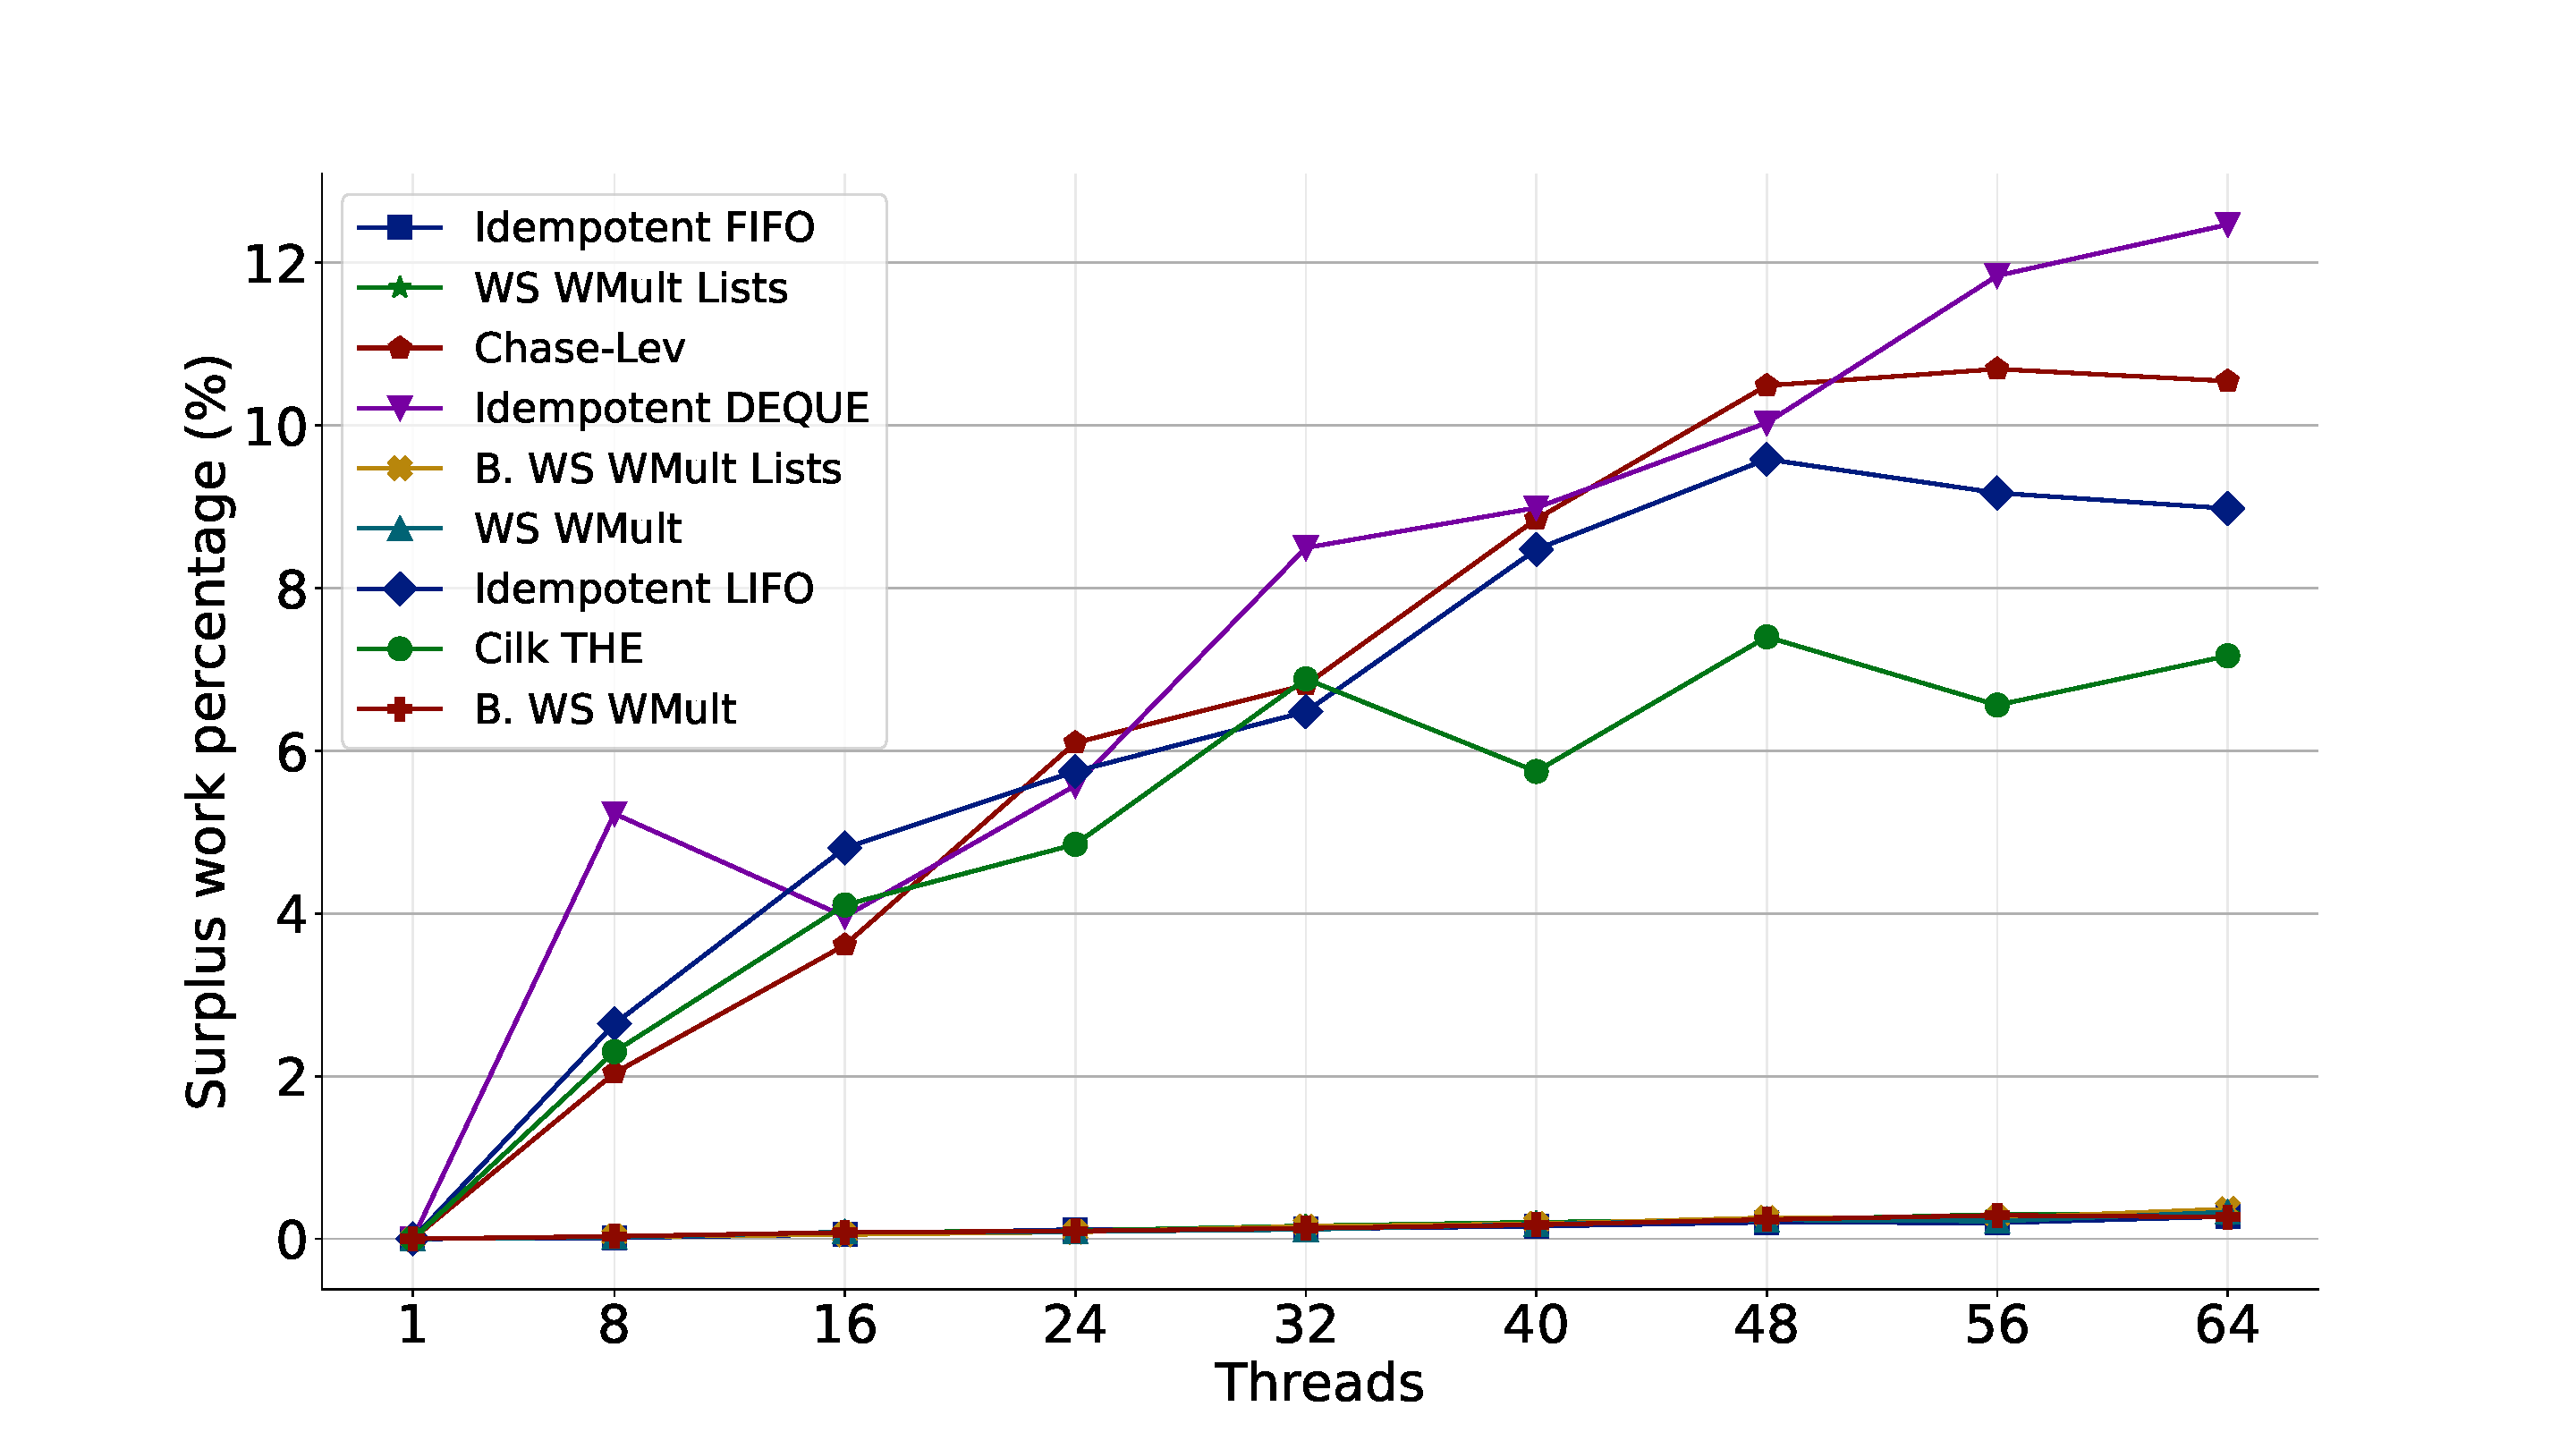
\includegraphics[width=0.48\textwidth]{contents/backmatter/evaluation/mult-torus_2d60_directed_256.pdf}
  }
  \subfloat[\label{fig:surplustorus2d60directed-appx:1000000}Surplus work: Directed Torus 2D 60\%. Initial size of 1,000,000 items]{
    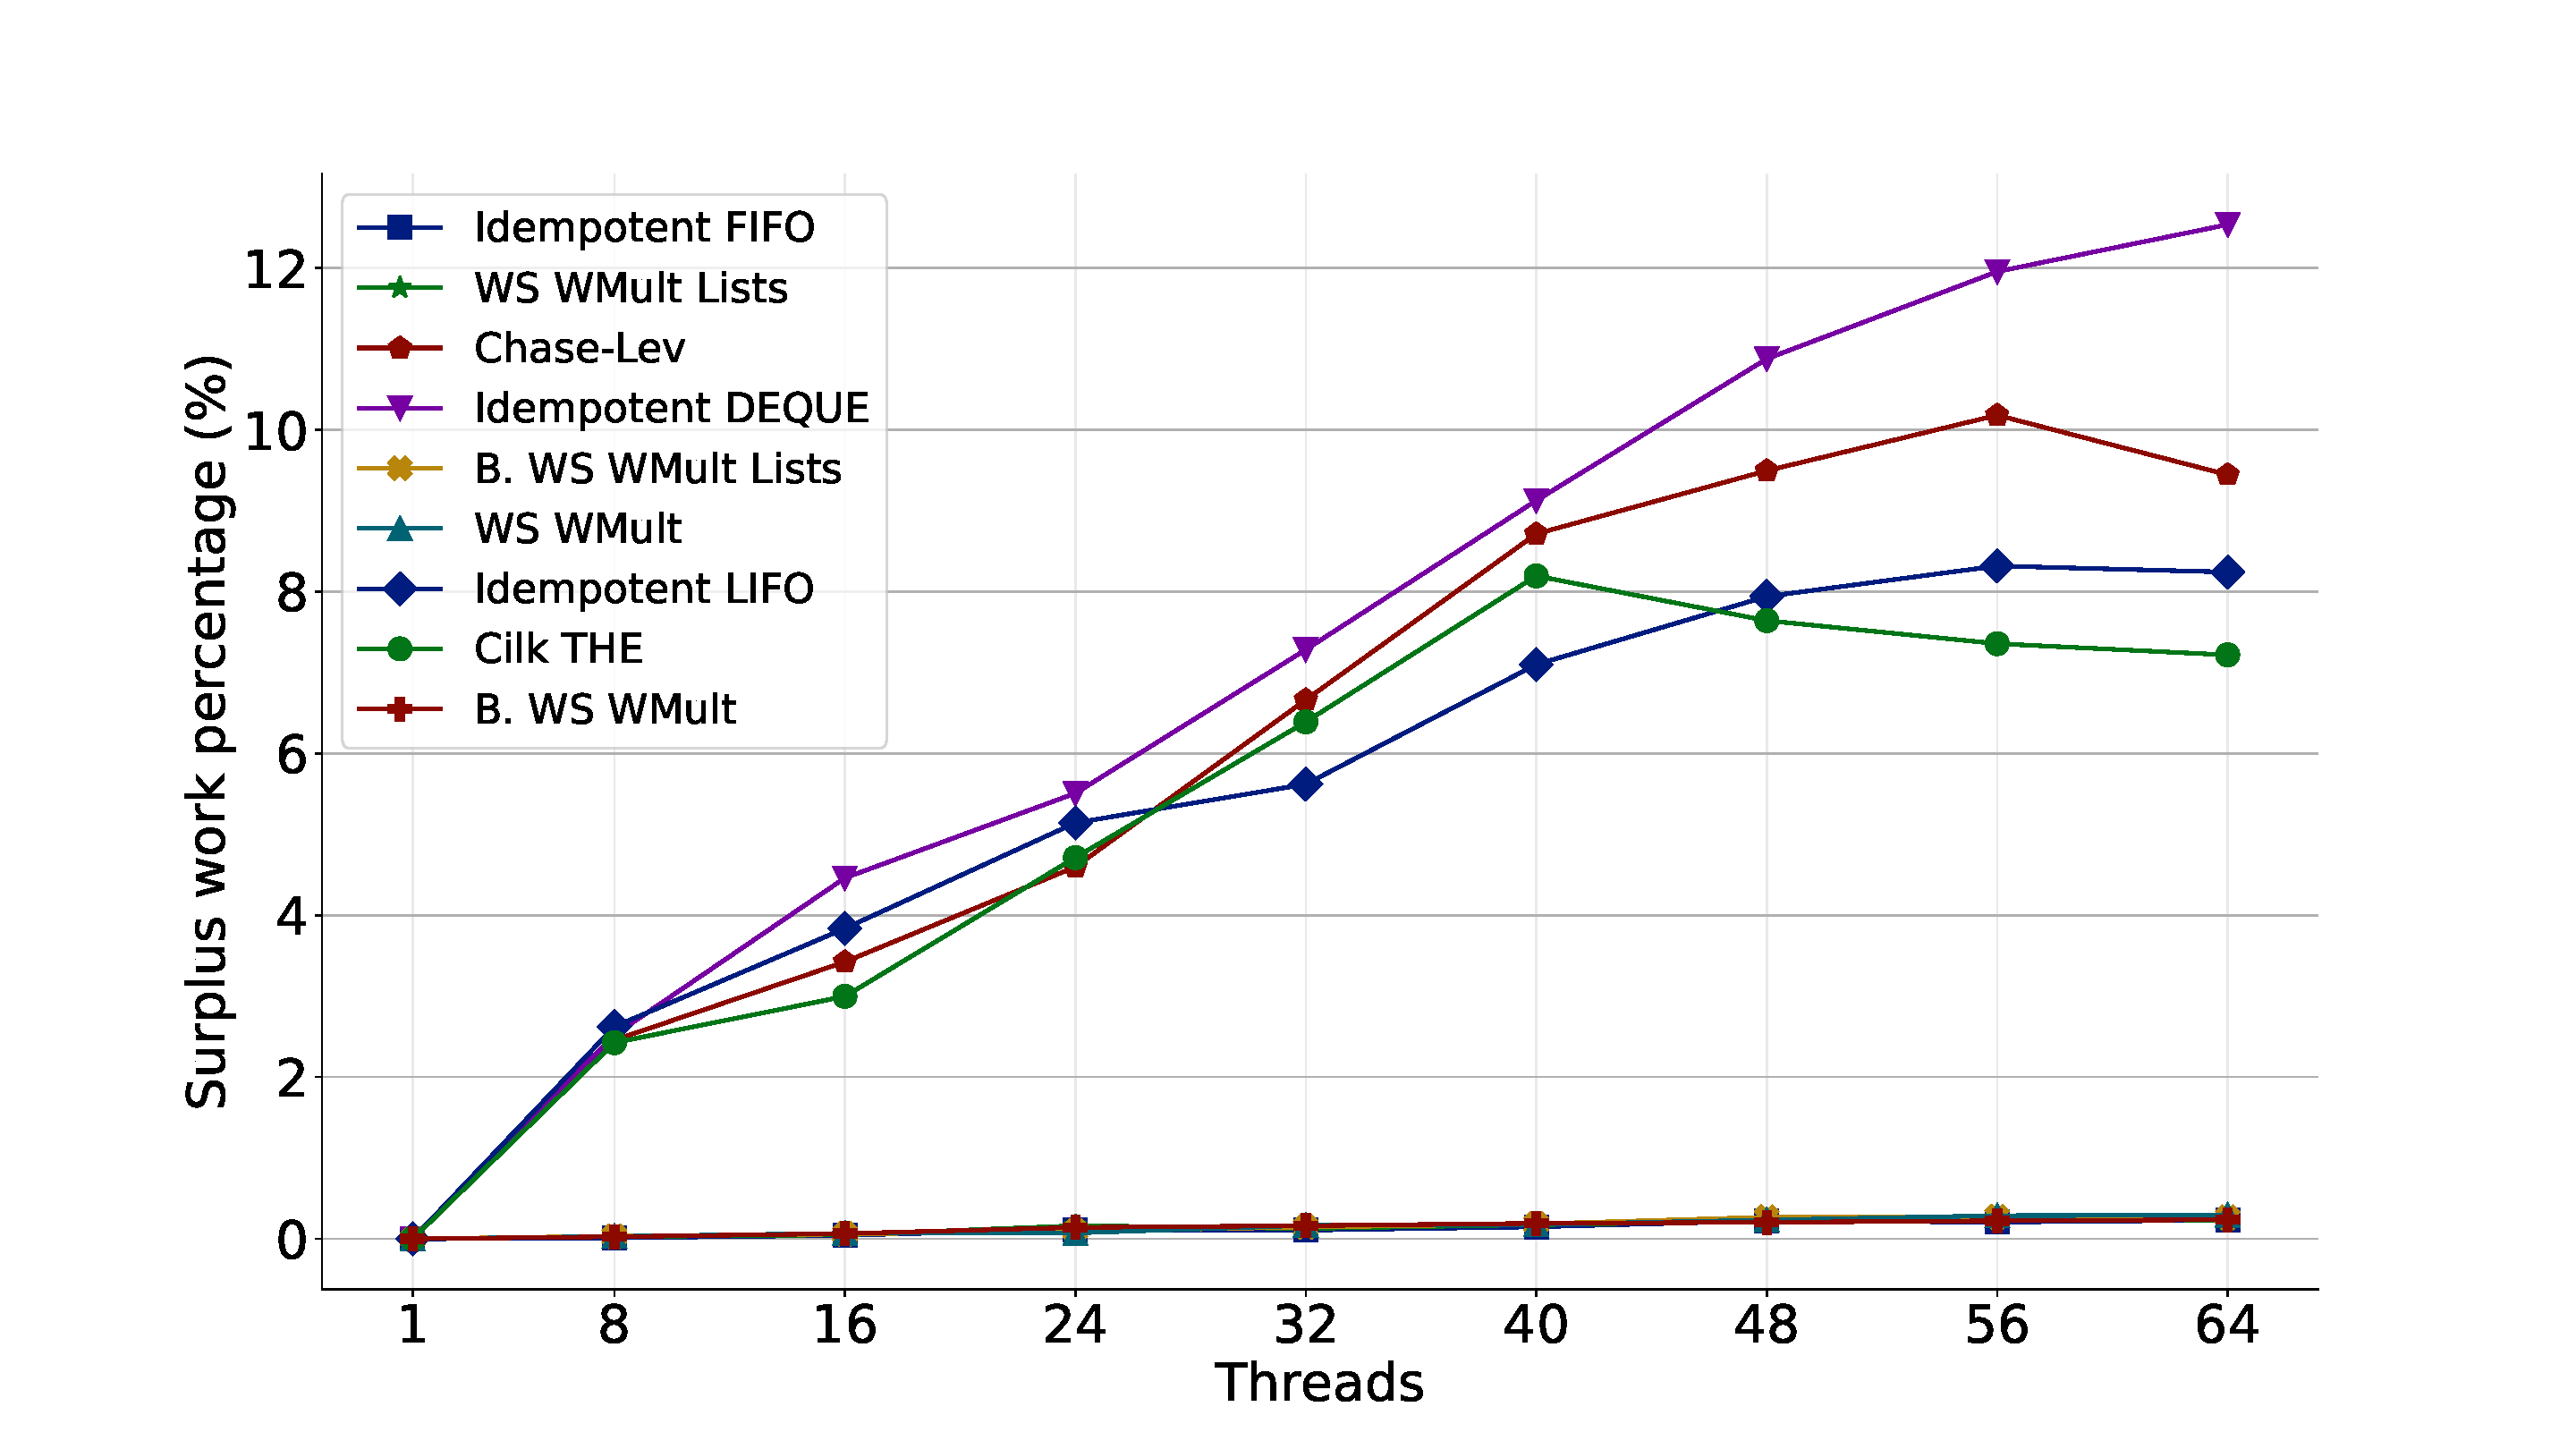
\includegraphics[width=0.48\textwidth]{contents/backmatter/evaluation/mult-torus_2d60_directed_1m.pdf}
  }

  \subfloat[\label{fig:surplustorus2d60undirected-appx:256}Surplus work: Undirected Torus 2D 60\%. Initial size of 256 items]{
    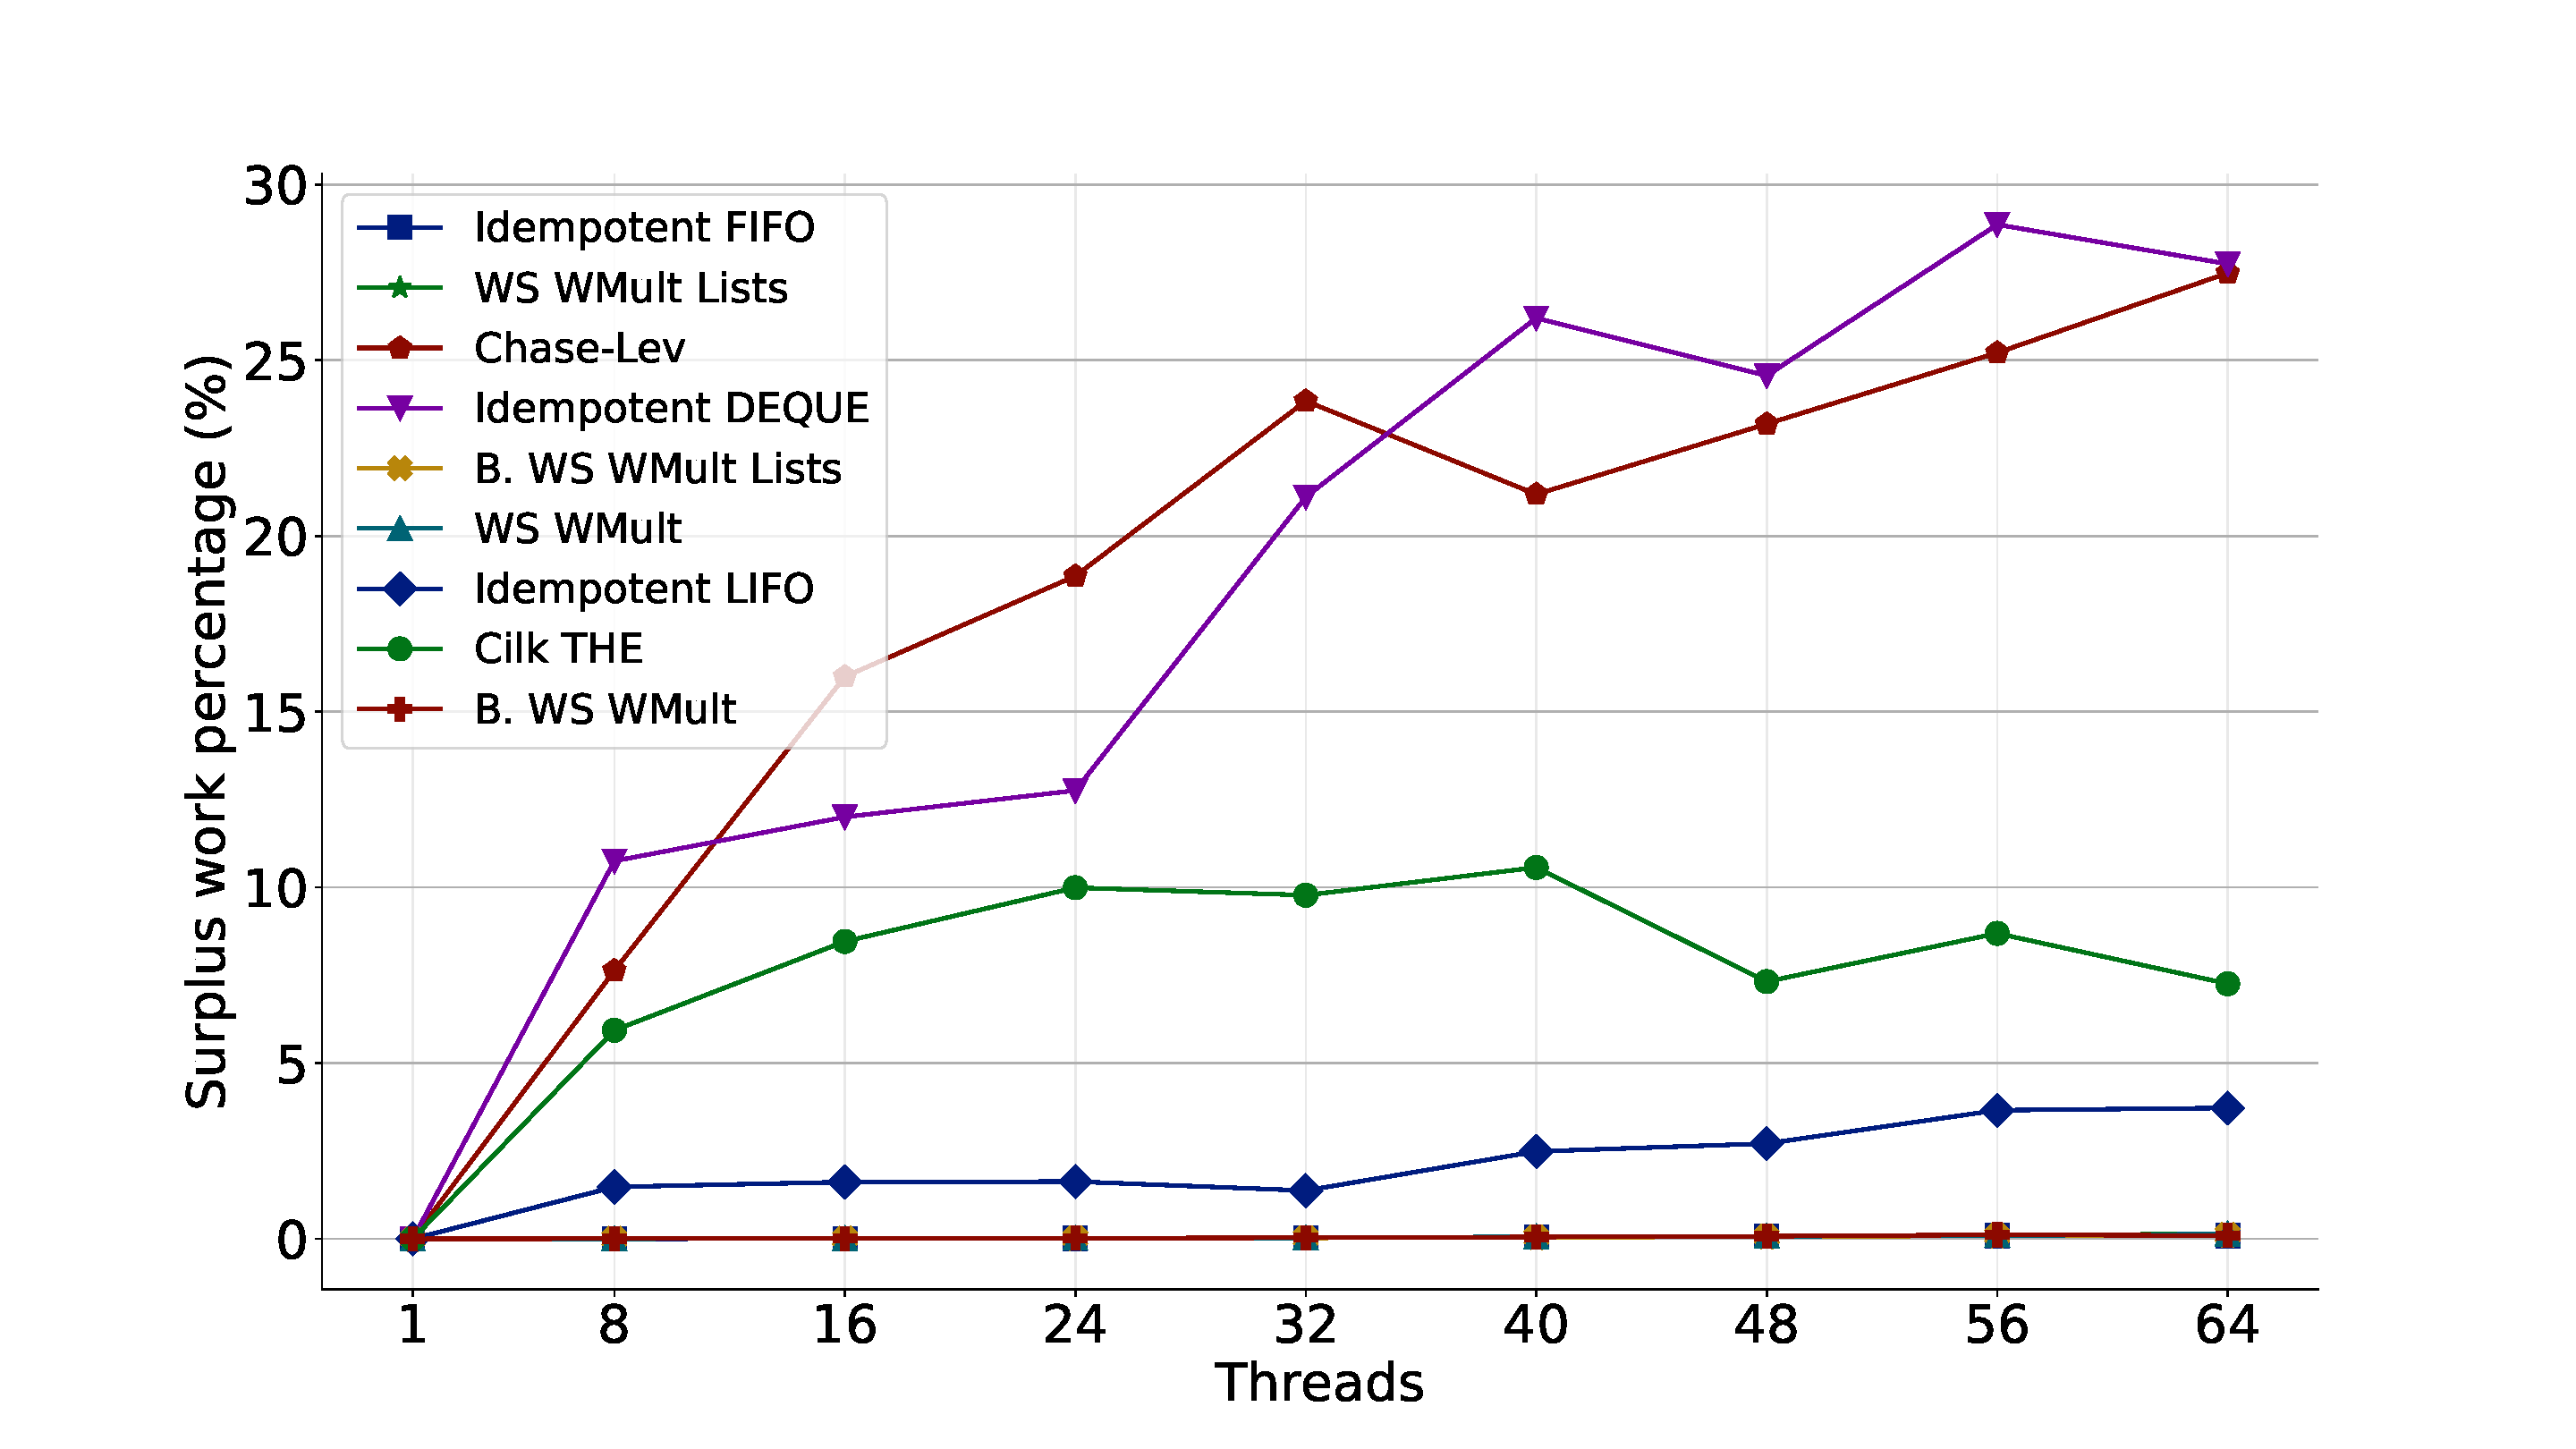
\includegraphics[width=0.48\textwidth]{contents/backmatter/evaluation/mult-torus_2d60_undirected_256.pdf}
  }
  \subfloat[\label{fig:surplustorus2d60undirected:1000000}Surplus work: Undirected Torus 2D 60\%. Initial size of 1,000,000 items]{
    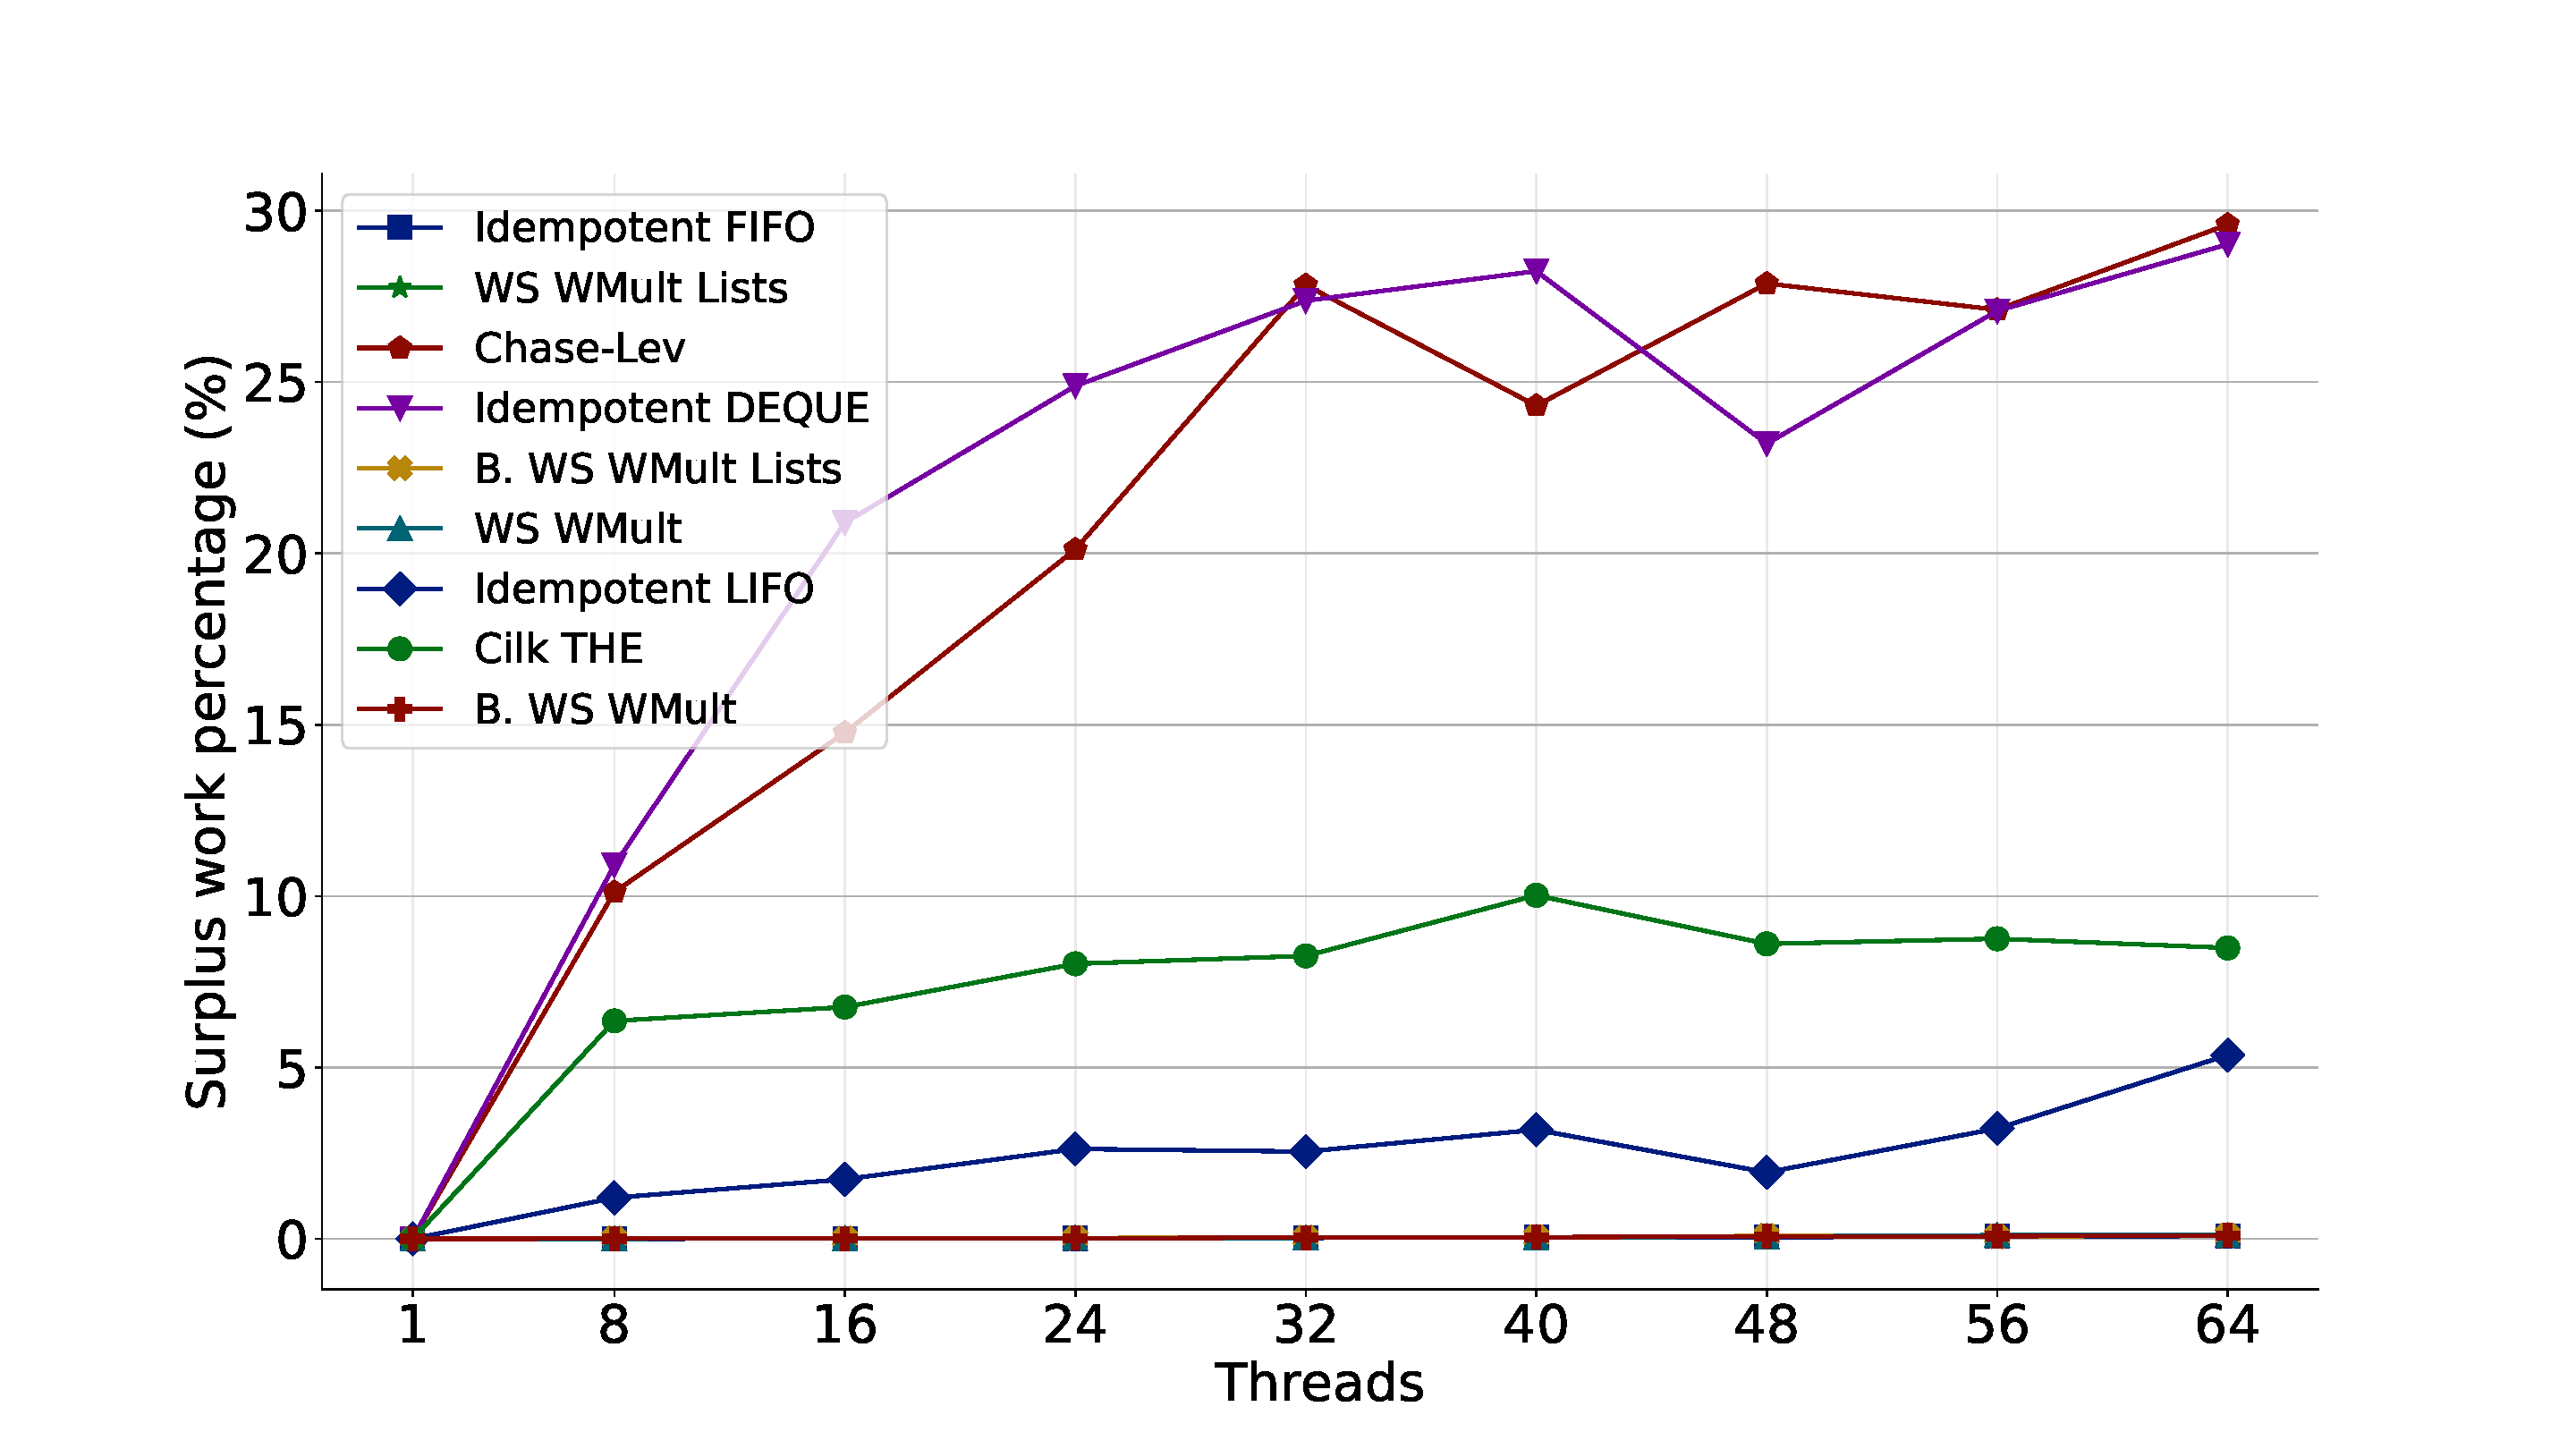
\includegraphics[width=0.48\textwidth]{contents/backmatter/evaluation/mult-torus_2d60_undirected_1m.pdf}
  }

  \caption{\label{fig:surplusgraphapplicationtorus2d60} Surplus work
    (percentage) of the experiments.  Surplus work: the difference between
    the total number of \Puts and the number of puts in sequential executions
    (i.e., $1,000,000$).}
\end{figure}

\begin{figure}[!ht]
  \subfloat[\label{fig:exec-surplustorus2d60directed-appx:256}Executed
  surplus work: Directed Torus 2D 60\%. Initial size of 256 items]{
    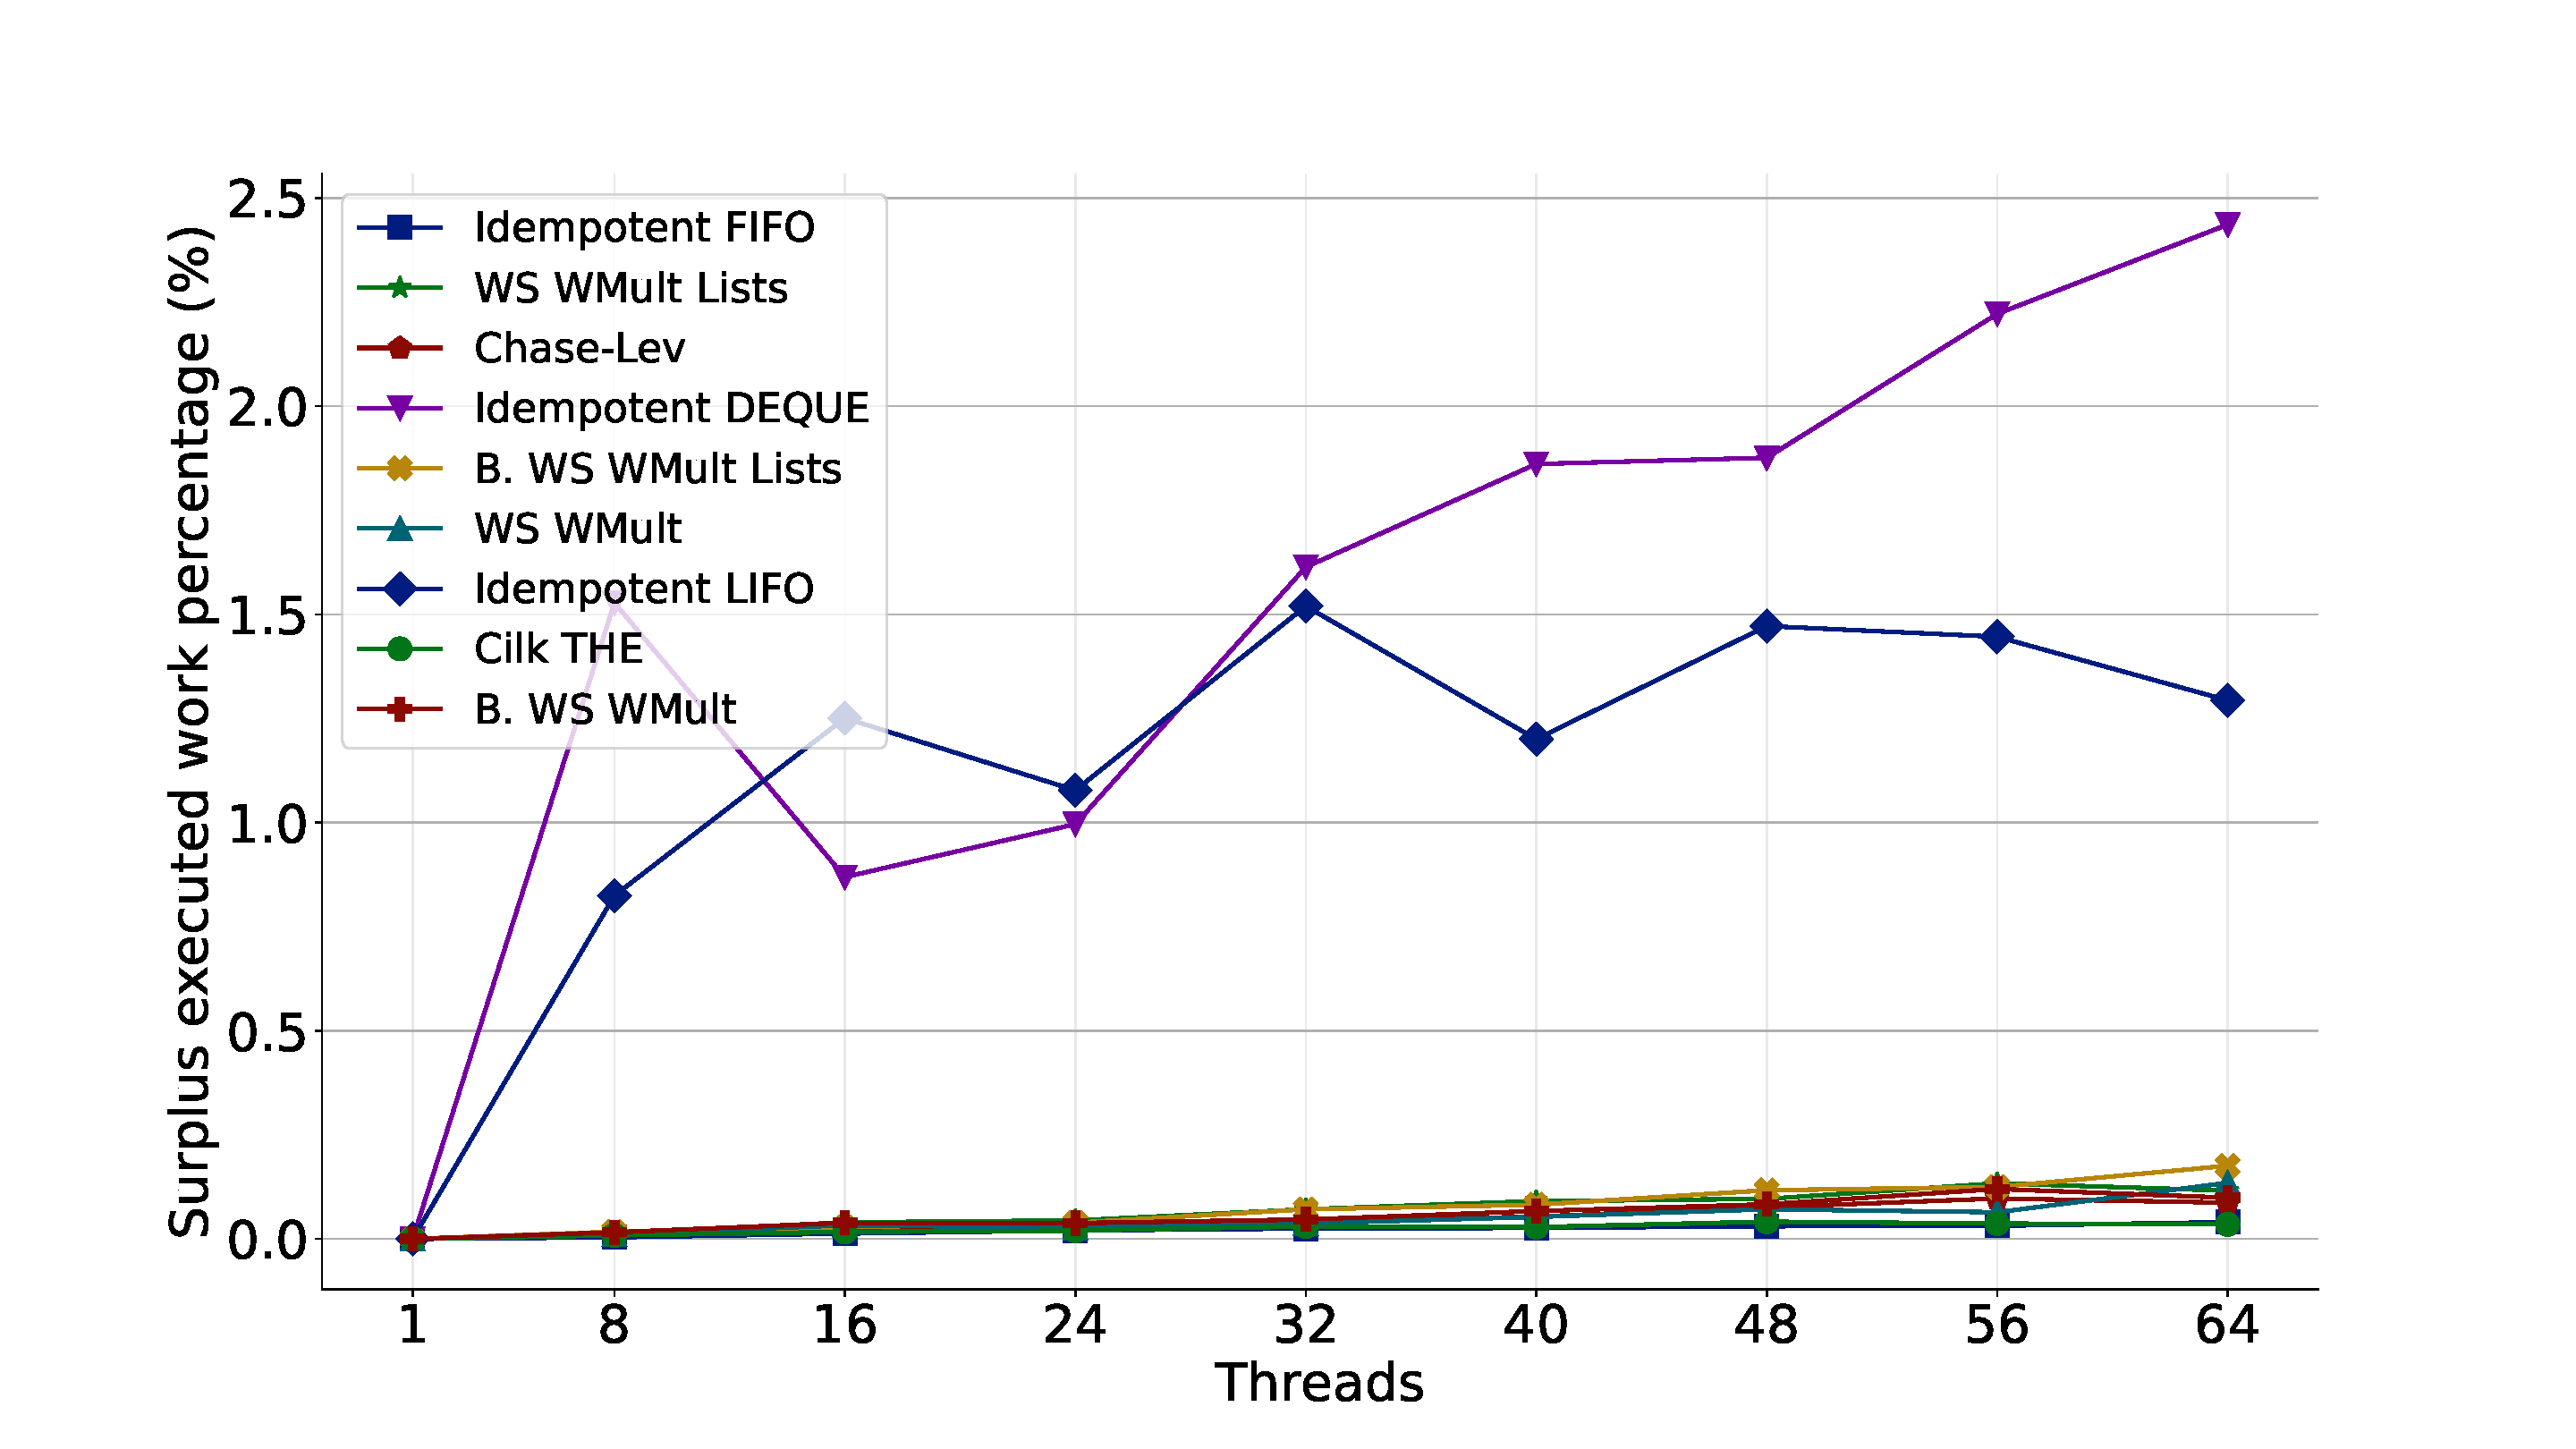
\includegraphics[width=0.48\textwidth]{contents/backmatter/evaluation/mult-exec-torus_2d60_directed_256.pdf}
  }
  \subfloat[\label{fig:exec-surplustorus2d60directed-appx:1000000}Executed
  surplus work: Directed Torus 2D 60\%. Initial size of 1,000,000 items]{
    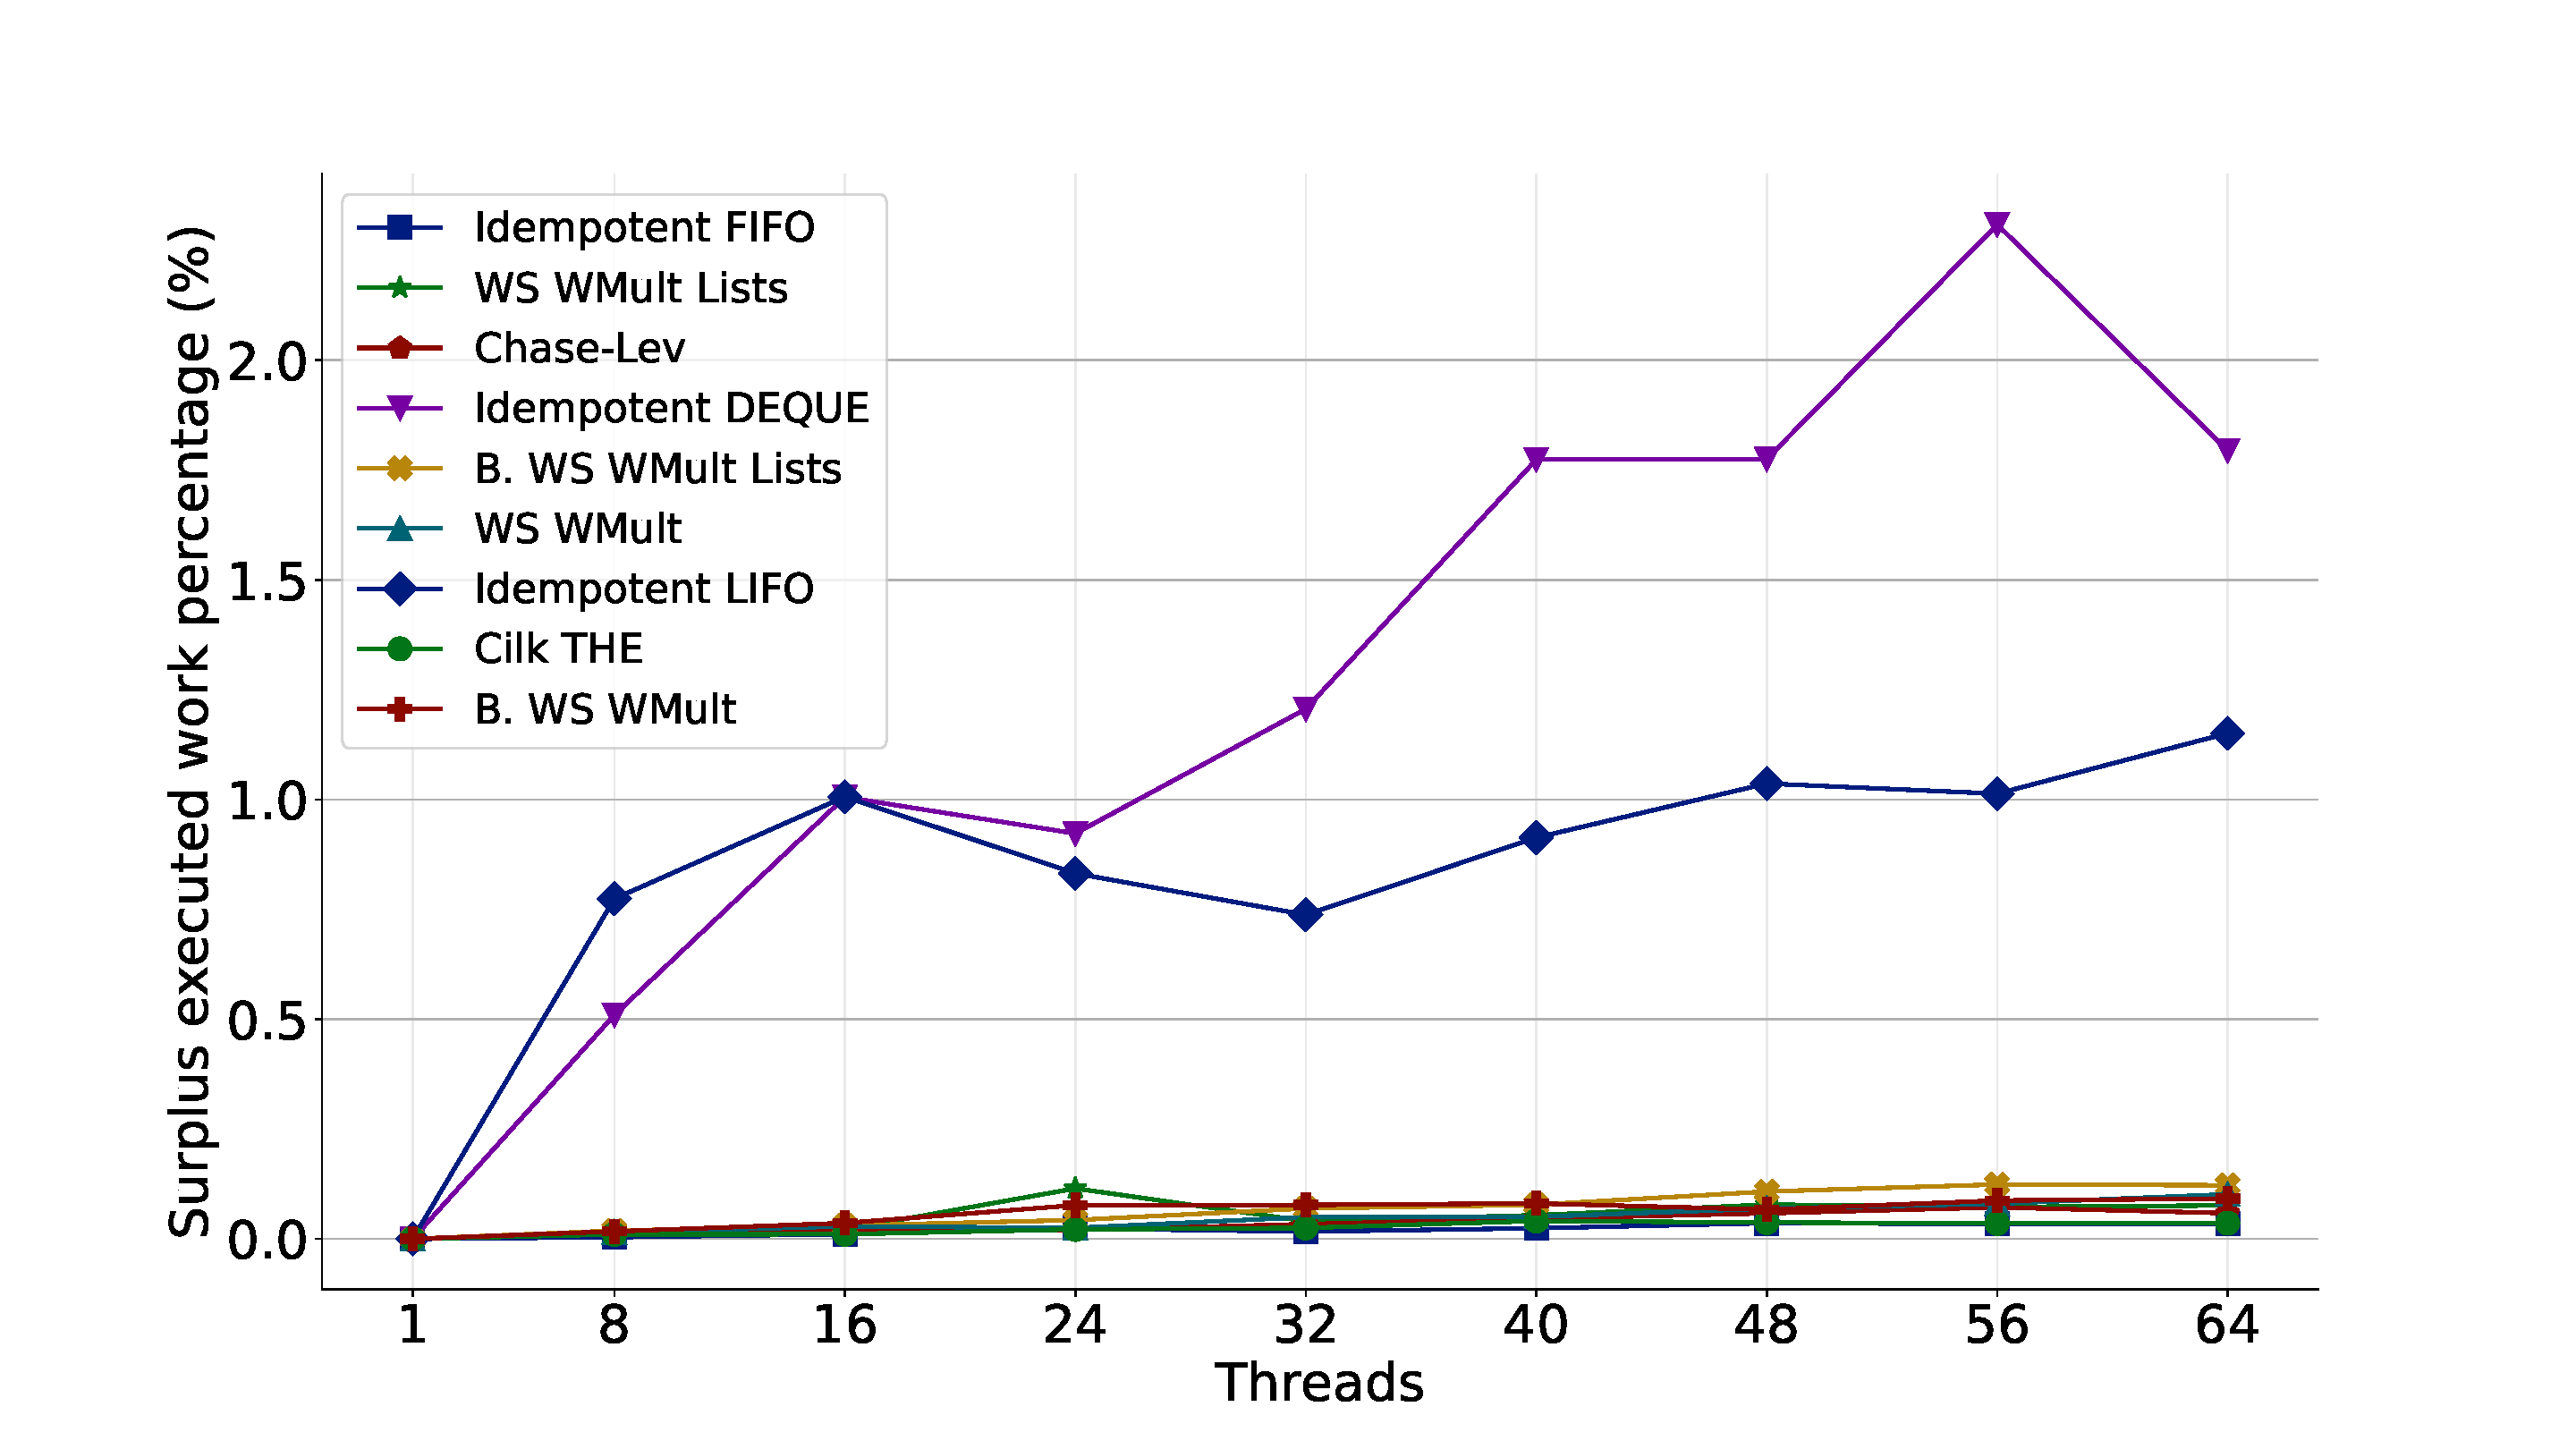
\includegraphics[width=0.48\textwidth]{contents/backmatter/evaluation/mult-exec-torus_2d60_directed_1m.pdf}
  }

  \subfloat[\label{fig:exec-surplustorus2d60undirected-appx:256}Executed
  Surplus work: Undirected Torus 2D 60\%. Initial size of 256 items]{
    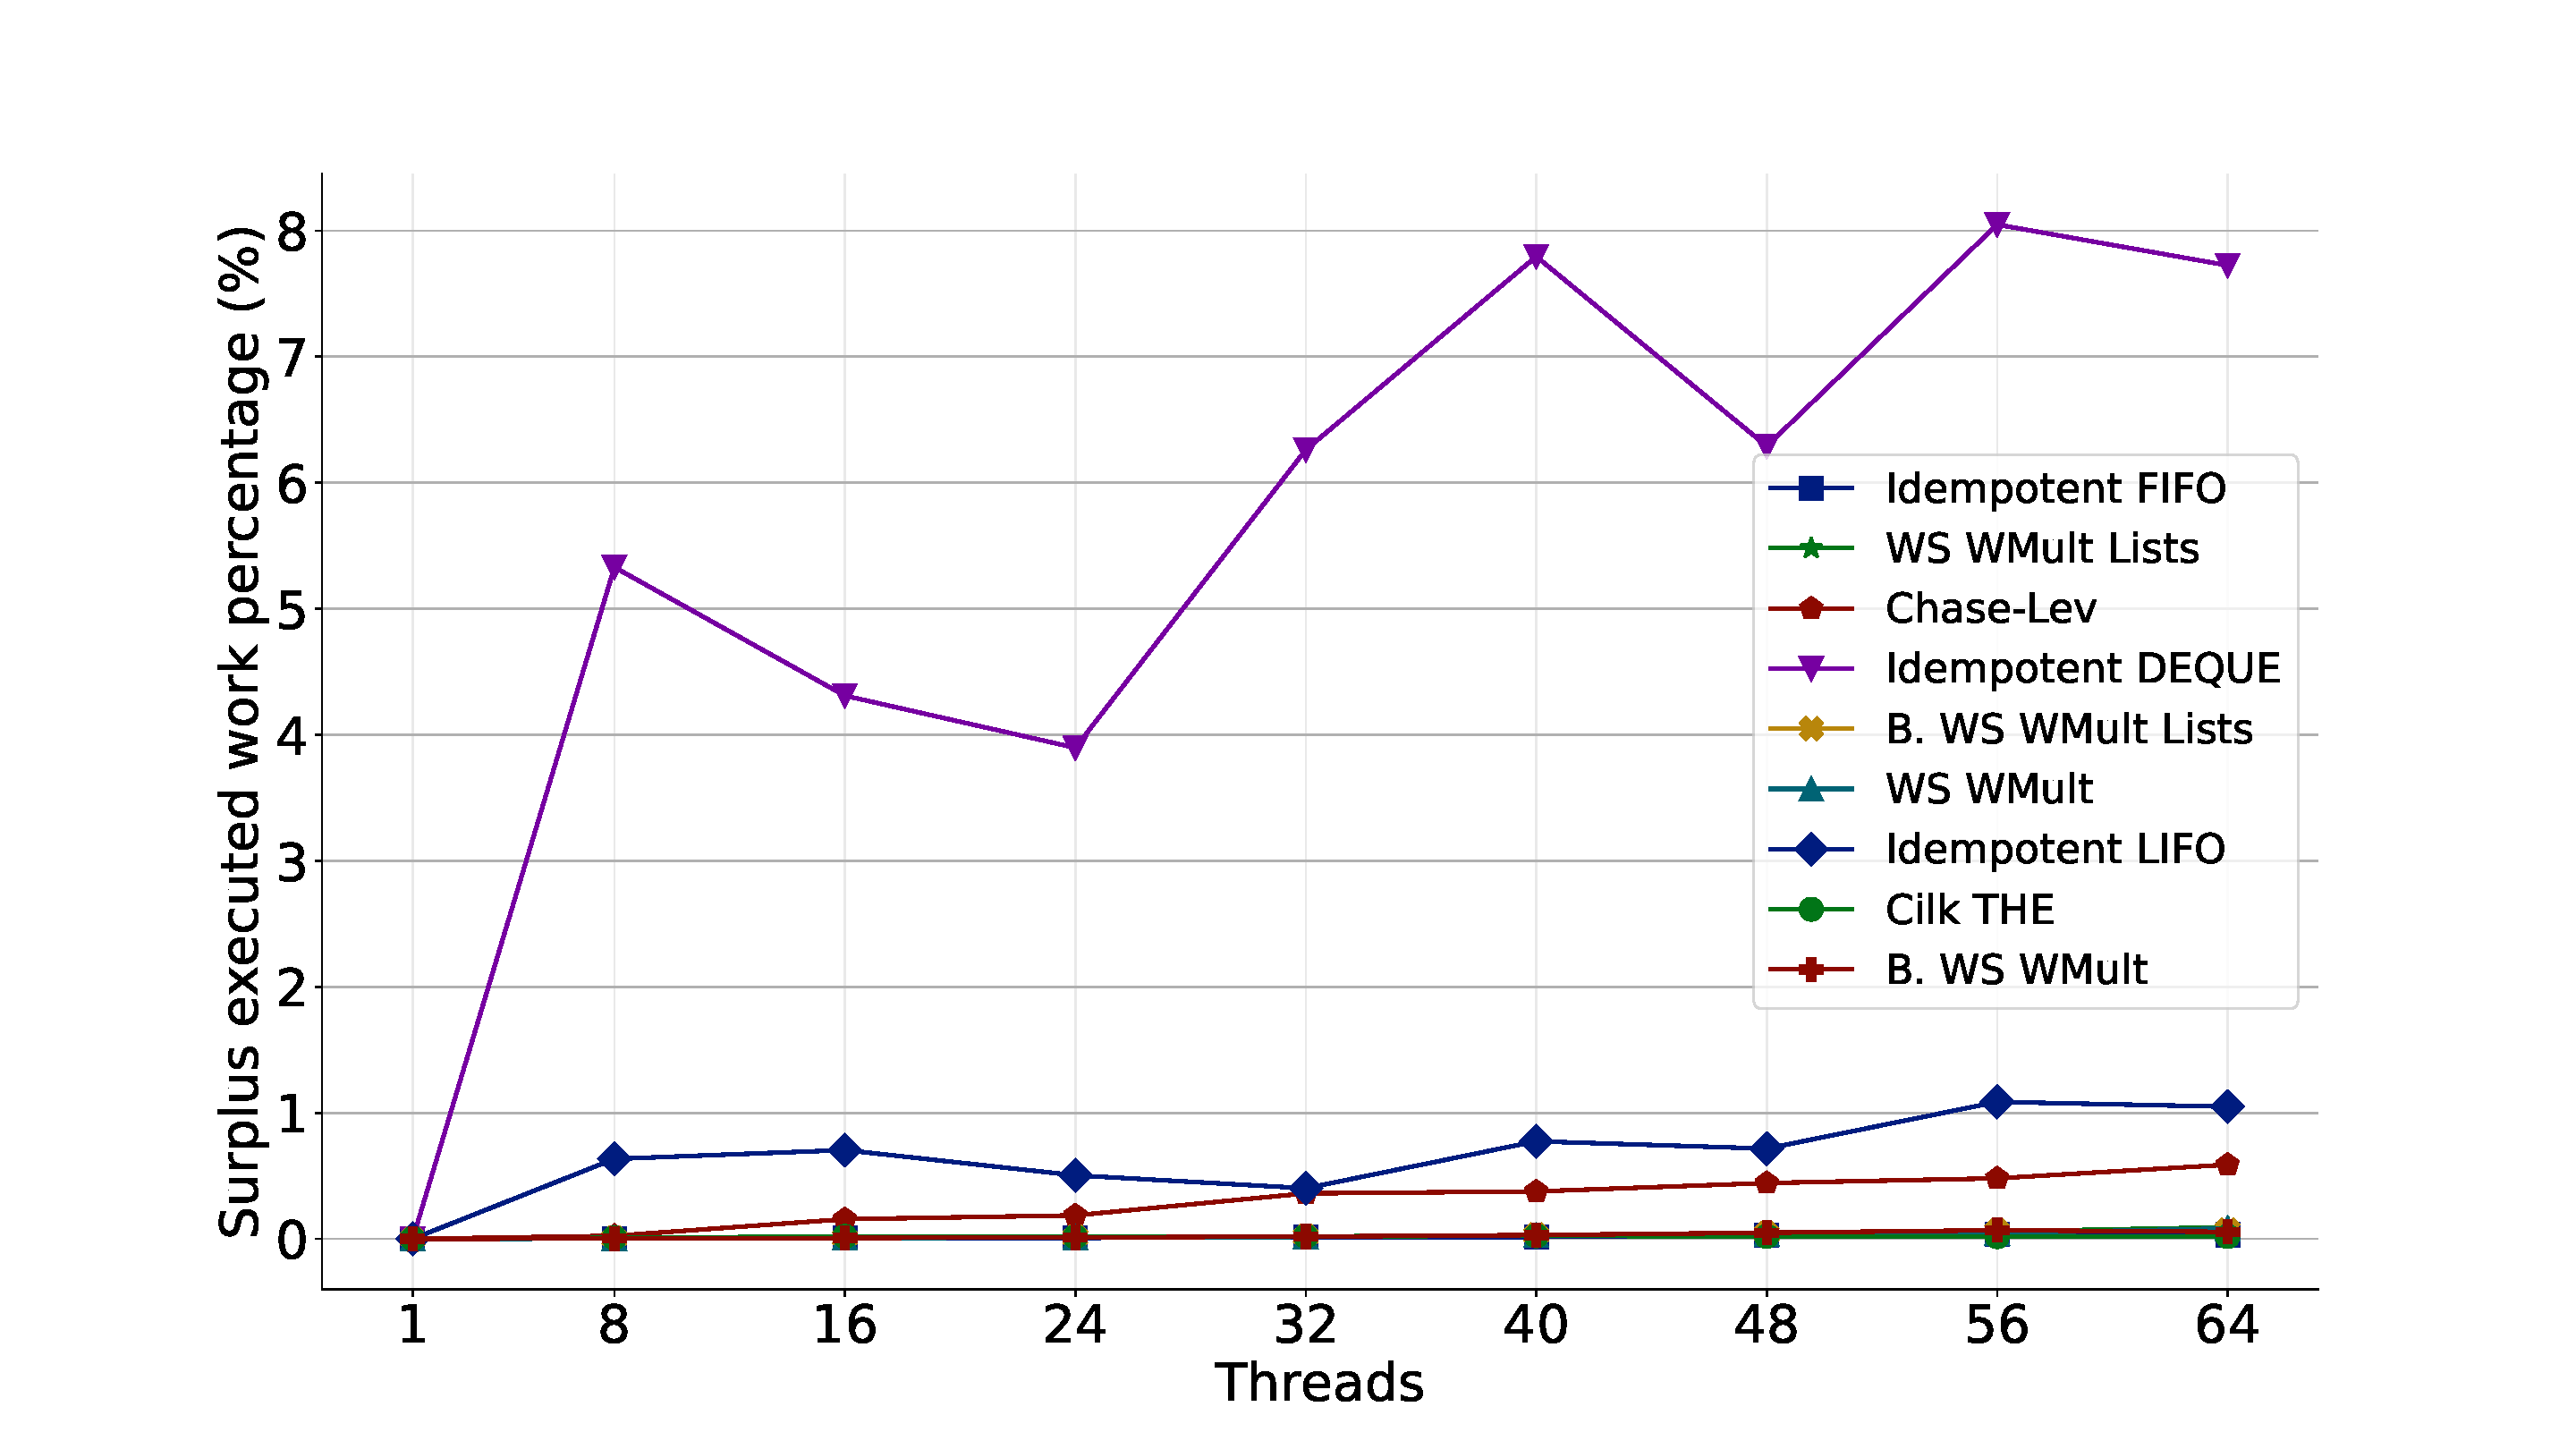
\includegraphics[width=0.48\textwidth]{contents/backmatter/evaluation/mult-exec-torus_2d60_undirected_256.pdf}
  }
  \subfloat[\label{fig:exec-surplustorus2d60undirected:1000000}Executed
  surplus work: Undirected Torus 2D 60\%. Initial size of 1,000,000 items]{
    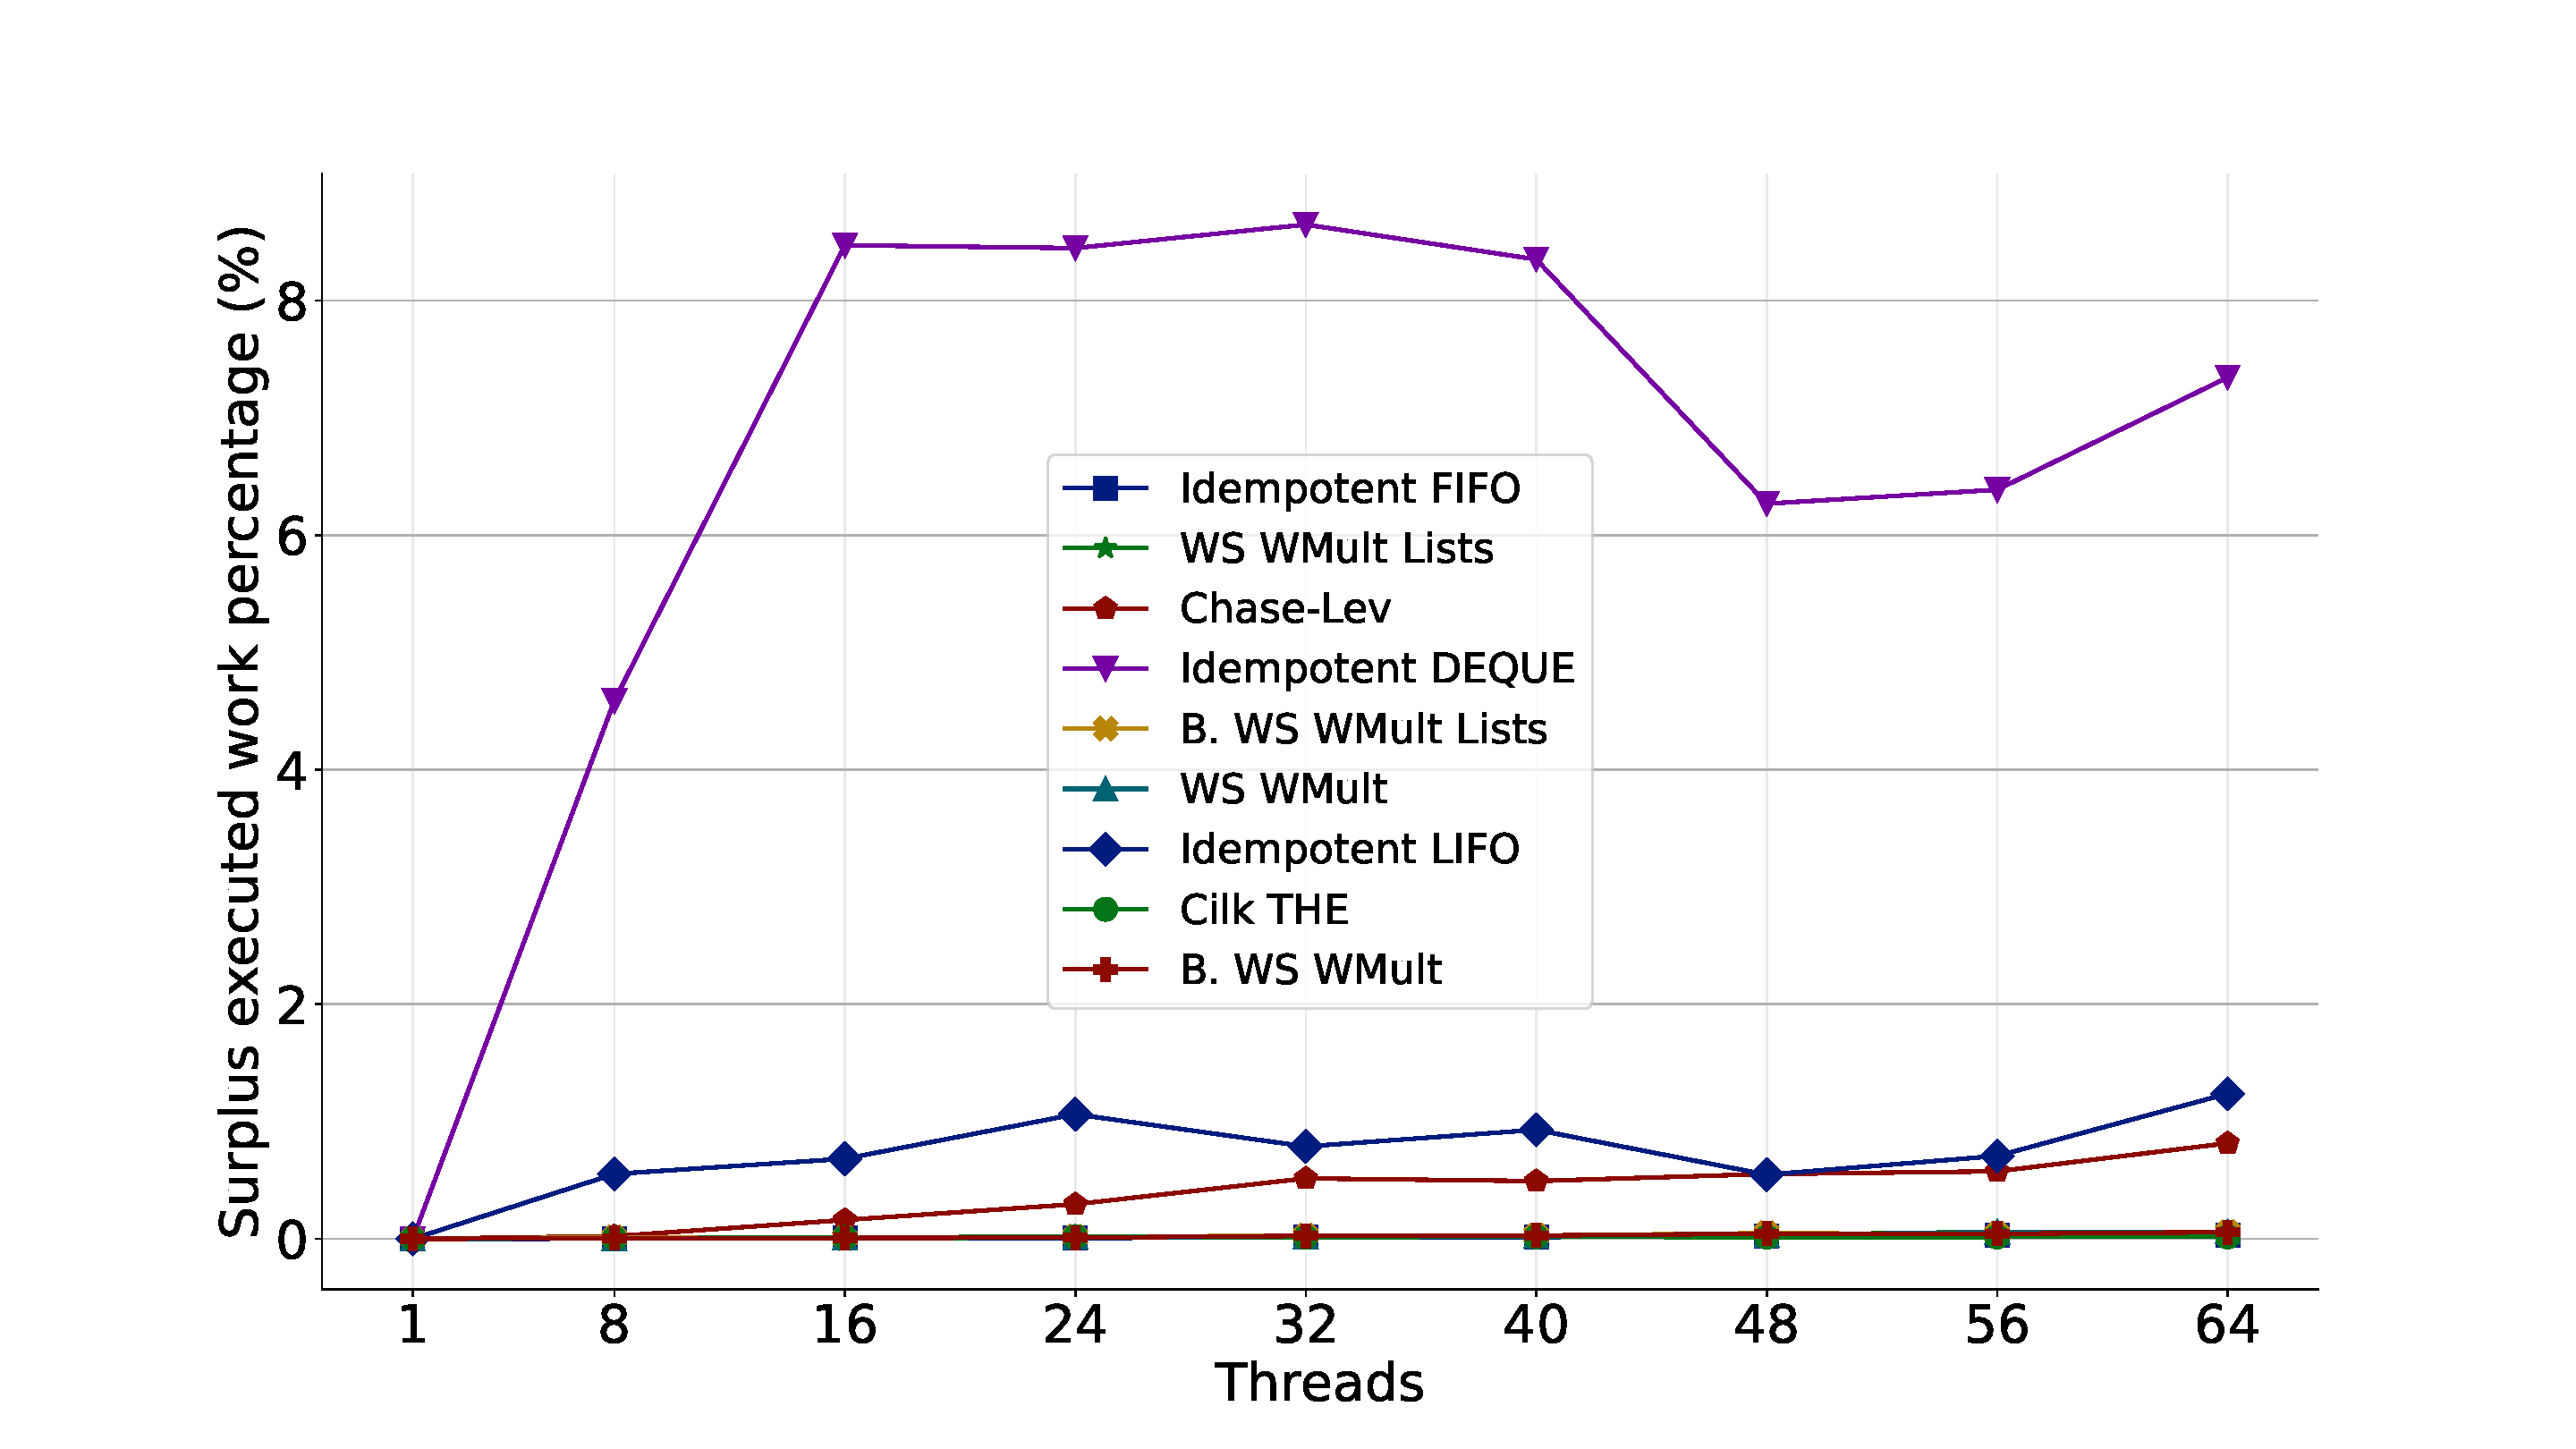
\includegraphics[width=0.48\textwidth]{contents/backmatter/evaluation/mult-exec-torus_2d60_undirected_1m.pdf}
  }

  \caption{\label{fig:exec-surplusgraphapplicationtorus2d60} Executed
    surplus work (percentage) of the experiments.  Surplus work: the
    difference between the total number of \Takes and the number of
    takes in sequential executions (i.e., $1,000,000$).  }
\end{figure}

\clearpage
\subsubsection{Directed Torus 3D. Initial size of 256 items.}
\begin{table}[!ht]
\centering
\resizebox{\textwidth}{!}{\begin{tabular}{lrrrrrrrrrrrrrrr}
\toprule
\textbf{Algorithm} & \multicolumn{5}{l}{Chase-Lev} & \multicolumn{5}{l}{Cilk THE} & \multicolumn{5}{l}{Idempotent LIFO} \\
\textbf{Operation} &       Puts &      Takes & Difference (\%) & Surplus (\%) & Executed Surplus (\%) &       Puts &      Takes & Difference (\%) & Surplus (\%) & Executed Surplus (\%) &            Puts &      Takes & Difference (\%) & Surplus (\%) & Executed Surplus (\%) \\
\textbf{Processes} & \multicolumn{4}{l}{} & \multicolumn{4}{l}{} & \multicolumn{4}{l}{}\\ \midrule
\textbf{1 } & 1000000.00 & 1000000.00 &           0.00 &        0.00 &                 0.00 & 1000000.00 & 1000000.00 &           0.00 &        0.00 &                 0.00 &      1000000.00 & 1000000.00 &           0.00 &        0.00 &                 0.00 \\
\textbf{8 } & 1518382.80 & 1002729.80 &          33.96 &       34.14 &                 0.27 & 1114649.40 & 1000045.60 &          10.28 &       10.29 &                 0.00 &      1098251.40 & 1026479.20 &           6.54 &        8.95 &                 2.58 \\
\textbf{16} & 1464633.60 & 1001836.80 &          31.60 &       31.72 &                 0.18 & 1139491.40 & 1000081.80 &          12.23 &       12.24 &                 0.01 &      1071382.80 & 1019950.80 &           4.80 &        6.66 &                 1.96 \\
\textbf{24} & 1488988.60 & 1001817.80 &          32.72 &       32.84 &                 0.18 & 1109569.60 & 1000095.40 &           9.87 &        9.87 &                 0.01 &      1066547.60 & 1019358.00 &           4.42 &        6.24 &                 1.90 \\
\textbf{28} & 1401148.20 & 1001090.00 &          28.55 &       28.63 &                 0.11 & 1118098.60 & 1000104.80 &          10.55 &       10.56 &                 0.01 &      1060865.60 & 1017061.20 &           4.13 &        5.74 &                 1.68 \\
\textbf{32} & 1428766.60 & 1001228.60 &          29.92 &       30.01 &                 0.12 & 1108755.80 & 1000092.20 &           9.80 &        9.81 &                 0.01 &      1058670.80 & 1016389.00 &           3.99 &        5.54 &                 1.61 \\
\textbf{40} & 1402662.80 & 1000773.60 &          28.65 &       28.71 &                 0.08 & 1118007.40 & 1000136.80 &          10.54 &       10.56 &                 0.01 &      1057805.80 & 1015497.60 &           4.00 &        5.46 &                 1.53 \\
\textbf{48} & 1419858.00 & 1001236.40 &          29.48 &       29.57 &                 0.12 & 1114775.00 & 1000101.40 &          10.29 &       10.30 &                 0.01 &      1068424.80 & 1018635.00 &           4.66 &        6.40 &                 1.83 \\
\textbf{56} & 1444332.80 & 1001655.20 &          30.65 &       30.76 &                 0.17 & 1121852.40 & 1000118.20 &          10.85 &       10.86 &                 0.01 &      1080560.40 & 1019777.80 &           5.63 &        7.46 &                 1.94 \\
\textbf{64} & 1428939.60 & 1002321.20 &          29.86 &       30.02 &                 0.23 & 1085480.00 & 1000122.40 &           7.86 &        7.87 &                 0.01 &      1080866.60 & 1023482.20 &           5.31 &        7.48 &                 2.29 \\
\bottomrule
\end{tabular}}
\label{difference-Torus_3D_directed-256-CHASELEV-CILK-IDEMPOTENT_LIFO}
\caption{The number of puts and takes performed during the
    spanning tree experiment on a Torus 3D directed graph with an initial size
    of 256 items is provided. The table presents data on the
    following algorithms: Chase-Lev, Cilk THE, and
    Idempotent LIFO. Furthermore, we present the percentage difference
    between the number of puts and takes for each available thread,
    relative to the total number of puts. Finally, also we show the
    "surplus" work, which is the difference of the total number of
    \Puts (Work to be scheduled) and the total number of \Puts in
    sequential executions (i.e., 1,000,000), and the "executed surplus
    work", which is the difference between the total number of \Takes
    (actual work executed) and the total of \Takes in sequential
    executions.}
\end{table}

\begin{table}[!ht]
\centering
\resizebox{\textwidth}{!}{\begin{tabular}{lrrrrrrrrrrrrrrr}
\toprule
\textbf{Algorithm} & \multicolumn{5}{l}{Idempotent DEQUE} & \multicolumn{5}{l}{Idempotent FIFO} & \multicolumn{5}{l}{WS WMult} \\
\textbf{Operation} &             Puts &      Takes & Difference (\%) & Surplus (\%) & Executed Surplus (\%) &            Puts &      Takes & Difference (\%) & Surplus (\%) & Executed Surplus (\%) &       Puts &      Takes & Difference (\%) & Surplus (\%) & Executed Surplus (\%) \\
\textbf{Processes} & \multicolumn{4}{l}{} & \multicolumn{4}{l}{} & \multicolumn{4}{l}{}\\ \midrule
\textbf{1 } &       1000000.00 & 1000000.00 &           0.00 &        0.00 &                 0.00 &      1000000.00 & 1000000.00 &           0.00 &        0.00 &                 0.00 & 1000000.00 & 1000000.00 &           0.00 &        0.00 &                 0.00 \\
\textbf{8 } &       1628867.80 & 1265167.80 &          22.33 &       38.61 &                20.96 &      1000414.20 & 1000398.60 &           0.00 &        0.04 &                 0.04 & 1000310.60 & 1000286.60 &           0.00 &        0.03 &                 0.03 \\
\textbf{16} &       1653954.80 & 1225914.00 &          25.88 &       39.54 &                18.43 &      1001764.20 & 1001724.80 &           0.00 &        0.18 &                 0.17 & 1002291.40 & 1001867.80 &           0.04 &        0.23 &                 0.19 \\
\textbf{24} &       1574299.20 & 1181708.80 &          24.94 &       36.48 &                15.38 &      1000944.60 & 1000684.60 &           0.03 &        0.09 &                 0.07 & 1001082.80 & 1000976.80 &           0.01 &        0.11 &                 0.10 \\
\textbf{28} &       1623697.60 & 1185717.00 &          26.97 &       38.41 &                15.66 &      1001322.40 & 1000952.00 &           0.04 &        0.13 &                 0.10 & 1001658.40 & 1000991.80 &           0.07 &        0.17 &                 0.10 \\
\textbf{32} &       1636044.00 & 1202424.20 &          26.50 &       38.88 &                16.83 &      1001061.40 & 1000741.60 &           0.03 &        0.11 &                 0.07 & 1001306.60 & 1000690.20 &           0.06 &        0.13 &                 0.07 \\
\textbf{40} &       1551282.60 & 1171691.40 &          24.47 &       35.54 &                14.65 &      1000989.80 & 1000481.40 &           0.05 &        0.10 &                 0.05 & 1001691.40 & 1000946.00 &           0.07 &        0.17 &                 0.09 \\
\textbf{48} &       1750071.00 & 1290436.00 &          26.26 &       42.86 &                22.51 &      1004021.80 & 1000727.80 &           0.33 &        0.40 &                 0.07 & 1003146.40 & 1001578.40 &           0.16 &        0.31 &                 0.16 \\
\textbf{56} &       1533304.40 & 1160251.40 &          24.33 &       34.78 &                13.81 &      1003050.00 & 1000705.60 &           0.23 &        0.30 &                 0.07 & 1003658.00 & 1001941.00 &           0.17 &        0.36 &                 0.19 \\
\textbf{64} &       1698806.60 & 1279848.40 &          24.66 &       41.14 &                21.87 &      1004193.20 & 1000838.80 &           0.33 &        0.42 &                 0.08 & 1005172.80 & 1002514.80 &           0.26 &        0.51 &                 0.25 \\
\bottomrule
\end{tabular}}
\label{difference-Torus_3D_directed-256-IDEMPOTENT_DEQUE-IDEMPOTENT_FIFO-WS_NC_MULT_OPT}
\caption{The number of puts and takes performed during the
    spanning tree experiment on a Torus 3D directed graph with an initial size
    of 256 items is provided. The table presents data on the
    following algorithms: Idempotent DEQUE, Idempotent FIFO, and
    WS WMult. Furthermore, we present the percentage difference
    between the number of puts and takes for each available thread,
    relative to the total number of puts. Finally, also we show the
    "surplus" work, which is the difference of the total number of
    \Puts (Work to be scheduled) and the total number of \Puts in
    sequential executions (i.e., 1,000,000), and the "executed surplus
    work", which is the difference between the total number of \Takes
    (actual work executed) and the total of \Takes in sequential
    executions.}
\end{table}

\begin{table}[!ht]
\centering
\resizebox{\textwidth}{!}{\begin{tabular}{lrrrrrrrrrrrrrrr}
\toprule
\textbf{Algorithm} & \multicolumn{5}{l}{B. WS WMult} & \multicolumn{5}{l}{WS WMult Lists} & \multicolumn{5}{l}{B. WS WMult Lists} \\
\textbf{Operation} &        Puts &      Takes & Difference (\%) & Surplus (\%) & Executed Surplus (\%) &           Puts &      Takes & Difference (\%) & Surplus (\%) & Executed Surplus (\%) &              Puts &      Takes & Difference (\%) & Surplus (\%) & Executed Surplus (\%) \\
\textbf{Processes} & \multicolumn{4}{l}{} & \multicolumn{4}{l}{} & \multicolumn{4}{l}{}\\ \midrule
\textbf{1 } &  1000000.00 & 1000000.00 &           0.00 &        0.00 &                 0.00 &     1000000.00 & 1000000.00 &           0.00 &        0.00 &                 0.00 &        1000000.00 & 1000000.00 &           0.00 &        0.00 &                 0.00 \\
\textbf{8 } &  1000512.20 & 1000367.40 &           0.01 &        0.05 &                 0.04 &     1000903.80 & 1000891.00 &           0.00 &        0.09 &                 0.09 &        1000700.40 & 1000686.60 &           0.00 &        0.07 &                 0.07 \\
\textbf{16} &  1000832.80 & 1000705.00 &           0.01 &        0.08 &                 0.07 &     1002111.00 & 1002073.40 &           0.00 &        0.21 &                 0.21 &        1001943.60 & 1001889.60 &           0.01 &        0.19 &                 0.19 \\
\textbf{24} &  1000730.80 & 1000478.40 &           0.03 &        0.07 &                 0.05 &     1001042.40 & 1000933.20 &           0.01 &        0.10 &                 0.09 &        1001613.60 & 1001425.80 &           0.02 &        0.16 &                 0.14 \\
\textbf{28} &  1002505.80 & 1001286.60 &           0.12 &        0.25 &                 0.13 &     1001728.20 & 1001212.20 &           0.05 &        0.17 &                 0.12 &        1001119.80 & 1000932.20 &           0.02 &        0.11 &                 0.09 \\
\textbf{32} &  1001376.00 & 1000711.20 &           0.07 &        0.14 &                 0.07 &     1001091.00 & 1000958.20 &           0.01 &        0.11 &                 0.10 &        1001096.80 & 1000720.60 &           0.04 &        0.11 &                 0.07 \\
\textbf{40} &  1003103.00 & 1001514.20 &           0.16 &        0.31 &                 0.15 &     1002010.40 & 1001200.20 &           0.08 &        0.20 &                 0.12 &        1001492.80 & 1001108.40 &           0.04 &        0.15 &                 0.11 \\
\textbf{48} &  1002573.80 & 1001210.40 &           0.14 &        0.26 &                 0.12 &     1002963.20 & 1001781.00 &           0.12 &        0.30 &                 0.18 &        1001636.40 & 1000914.20 &           0.07 &        0.16 &                 0.09 \\
\textbf{56} &  1006062.00 & 1002658.60 &           0.34 &        0.60 &                 0.27 &     1003712.80 & 1002003.20 &           0.17 &        0.37 &                 0.20 &        1004573.40 & 1001954.40 &           0.26 &        0.46 &                 0.20 \\
\textbf{64} &  1006329.00 & 1002971.80 &           0.33 &        0.63 &                 0.30 &     1007954.20 & 1003634.60 &           0.43 &        0.79 &                 0.36 &        1004020.40 & 1001714.00 &           0.23 &        0.40 &                 0.17 \\
\bottomrule
\end{tabular}}
\label{difference-Torus_3D_directed-256-B_WS_NC_MULT_OPT-WS_NC_MULT_LA_OPT-B_WS_NC_MULT_LA_OPT}
\caption{The number of puts and takes performed during the
    spanning tree experiment on a Torus 3D directed graph with an initial size
    of 256 items is provided. The table presents data on the
    following algorithms: B. WS WMult, WS WMult Lists, and
    B. WS WMult Lists. Furthermore, we present the percentage difference
    between the number of puts and takes for each available thread,
    relative to the total number of puts. Finally, also we show the
    "surplus" work, which is the difference of the total number of
    \Puts (Work to be scheduled) and the total number of \Puts in
    sequential executions (i.e., 1,000,000), and the "executed surplus
    work", which is the difference between the total number of \Takes
    (actual work executed) and the total of \Takes in sequential
    executions.}
\end{table}

\clearpage
\subsubsection{Directed Torus 3D. Initial size of  1,000,000 items.}
\begin{table}[!ht]
\centering
\resizebox{\textwidth}{!}{\begin{tabular}{lrrrrrrrrrrrrrrr}
\toprule
\textbf{Algorithm} & \multicolumn{5}{l}{Chase-Lev} & \multicolumn{5}{l}{Cilk THE} & \multicolumn{5}{l}{Idempotent LIFO} \\
\textbf{Operation} &       Puts &      Takes & Difference (\%) & Surplus (\%) & Executed Surplus (\%) &       Puts &      Takes & Difference (\%) & Surplus (\%) & Executed Surplus (\%) &            Puts &      Takes & Difference (\%) & Surplus (\%) & Executed Surplus (\%) \\
\textbf{Processes} & \multicolumn{4}{l}{} & \multicolumn{4}{l}{} & \multicolumn{4}{l}{}\\ \midrule
\textbf{1 } & 1000000.00 & 1000000.00 &           0.00 &        0.00 &                 0.00 & 1000000.00 & 1000000.00 &           0.00 &        0.00 &                 0.00 &      1000000.00 & 1000000.00 &           0.00 &        0.00 &                 0.00 \\
\textbf{8 } & 1372395.20 & 1001635.40 &          27.02 &       27.13 &                 0.16 & 1122614.60 & 1000088.20 &          10.91 &       10.92 &                 0.01 &      1059276.80 & 1024567.20 &           3.28 &        5.60 &                 2.40 \\
\textbf{16} & 1433214.60 & 1000323.40 &          30.20 &       30.23 &                 0.03 & 1127121.80 & 1000090.60 &          11.27 &       11.28 &                 0.01 &      1057170.20 & 1021495.00 &           3.37 &        5.41 &                 2.10 \\
\textbf{24} & 1448832.80 & 1000533.80 &          30.94 &       30.98 &                 0.05 & 1114541.40 & 1000115.80 &          10.27 &       10.28 &                 0.01 &      1059802.20 & 1020125.00 &           3.74 &        5.64 &                 1.97 \\
\textbf{28} & 1385503.60 & 1001000.20 &          27.75 &       27.82 &                 0.10 & 1111023.60 & 1000073.40 &           9.99 &        9.99 &                 0.01 &      1064373.40 & 1019316.40 &           4.23 &        6.05 &                 1.90 \\
\textbf{32} & 1416874.80 & 1000771.80 &          29.37 &       29.42 &                 0.08 & 1101505.00 & 1000085.40 &           9.21 &        9.22 &                 0.01 &      1060945.20 & 1019519.00 &           3.90 &        5.74 &                 1.91 \\
\textbf{40} & 1419027.00 & 1000730.20 &          29.48 &       29.53 &                 0.07 & 1106658.20 & 1000147.20 &           9.62 &        9.64 &                 0.01 &      1059128.00 & 1017581.40 &           3.92 &        5.58 &                 1.73 \\
\textbf{48} & 1342022.00 & 1000699.40 &          25.43 &       25.49 &                 0.07 & 1122954.40 & 1000110.60 &          10.94 &       10.95 &                 0.01 &      1066871.60 & 1019310.20 &           4.46 &        6.27 &                 1.89 \\
\textbf{56} & 1378406.80 & 1000663.00 &          27.40 &       27.45 &                 0.07 & 1095288.80 & 1000113.60 &           8.69 &        8.70 &                 0.01 &      1065900.60 & 1017963.20 &           4.50 &        6.18 &                 1.76 \\
\textbf{64} & 1349161.60 & 1001019.60 &          25.80 &       25.88 &                 0.10 & 1107860.00 & 1000147.20 &           9.72 &        9.74 &                 0.01 &      1067699.60 & 1018627.60 &           4.60 &        6.34 &                 1.83 \\
\bottomrule
\end{tabular}}
\label{difference-Torus_3D_directed-1000000-CHASELEV-CILK-IDEMPOTENT_LIFO}
\caption{The number of puts and takes performed during the
    spanning tree experiment on a Torus 3D directed graph with an initial size
    of 1000000 items is provided. The table presents data on the
    following algorithms: Chase-Lev, Cilk THE, and
    Idempotent LIFO. Furthermore, we present the percentage difference
    between the number of puts and takes for each available thread,
    relative to the total number of puts. Finally, also we show the
    "surplus" work, which is the difference of the total number of
    \Puts (Work to be scheduled) and the total number of \Puts in
    sequential executions (i.e., 1,000,000), and the "executed surplus
    work", which is the difference between the total number of \Takes
    (actual work executed) and the total of \Takes in sequential
    executions.}
\end{table}

\begin{table}[!ht]
\centering
\resizebox{\textwidth}{!}{\begin{tabular}{lrrrrrrrrrrrrrrr}
\toprule
\textbf{Algorithm} & \multicolumn{5}{l}{Idempotent DEQUE} & \multicolumn{5}{l}{Idempotent FIFO} & \multicolumn{5}{l}{WS WMult} \\
\textbf{Operation} &             Puts &      Takes & Difference (\%) & Surplus (\%) & Executed Surplus (\%) &            Puts &      Takes & Difference (\%) & Surplus (\%) & Executed Surplus (\%) &       Puts &      Takes & Difference (\%) & Surplus (\%) & Executed Surplus (\%) \\
\textbf{Processes} & \multicolumn{4}{l}{} & \multicolumn{4}{l}{} & \multicolumn{4}{l}{}\\ \midrule
\textbf{1 } &       1000000.00 & 1000000.00 &           0.00 &        0.00 &                 0.00 &      1000000.00 & 1000000.00 &           0.00 &        0.00 &                 0.00 & 1000000.00 & 1000000.00 &           0.00 &        0.00 &                 0.00 \\
\textbf{8 } &       1411172.60 & 1145740.00 &          18.81 &       29.14 &                12.72 &      1000993.40 & 1000972.00 &           0.00 &        0.10 &                 0.10 & 1000764.60 & 1000752.00 &           0.00 &        0.08 &                 0.08 \\
\textbf{16} &       1687686.20 & 1255514.00 &          25.61 &       40.75 &                20.35 &      1002500.00 & 1002471.40 &           0.00 &        0.25 &                 0.25 & 1001408.00 & 1001336.40 &           0.01 &        0.14 &                 0.13 \\
\textbf{24} &       1696765.80 & 1224102.60 &          27.86 &       41.06 &                18.31 &      1001302.40 & 1001198.80 &           0.01 &        0.13 &                 0.12 & 1001260.00 & 1001009.60 &           0.03 &        0.13 &                 0.10 \\
\textbf{28} &       1641905.20 & 1184651.60 &          27.85 &       39.10 &                15.59 &      1001690.80 & 1001322.80 &           0.04 &        0.17 &                 0.13 & 1002090.00 & 1001566.00 &           0.05 &        0.21 &                 0.16 \\
\textbf{32} &       1603087.60 & 1171833.40 &          26.90 &       37.62 &                14.66 &      1001271.80 & 1000695.20 &           0.06 &        0.13 &                 0.07 & 1001681.60 & 1001116.40 &           0.06 &        0.17 &                 0.11 \\
\textbf{40} &       1410310.80 & 1091270.80 &          22.62 &       29.09 &                 8.36 &      1000720.40 & 1000444.60 &           0.03 &        0.07 &                 0.04 & 1004530.20 & 1002401.60 &           0.21 &        0.45 &                 0.24 \\
\textbf{48} &       1560914.00 & 1159006.60 &          25.75 &       35.93 &                13.72 &      1002612.60 & 1001084.40 &           0.15 &        0.26 &                 0.11 & 1003340.60 & 1001872.80 &           0.15 &        0.33 &                 0.19 \\
\textbf{56} &       1593918.80 & 1199605.40 &          24.74 &       37.26 &                16.64 &      1003855.60 & 1000798.40 &           0.30 &        0.38 &                 0.08 & 1005926.20 & 1003121.40 &           0.28 &        0.59 &                 0.31 \\
\textbf{64} &       1519171.60 & 1166243.60 &          23.23 &       34.17 &                14.25 &      1003976.00 & 1000806.60 &           0.32 &        0.40 &                 0.08 & 1004574.40 & 1002374.00 &           0.22 &        0.46 &                 0.24 \\
\bottomrule
\end{tabular}}
\label{difference-Torus_3D_directed-1000000-IDEMPOTENT_DEQUE-IDEMPOTENT_FIFO-WS_NC_MULT_OPT}
\caption{The number of puts and takes performed during the
    spanning tree experiment on a Torus 3D directed graph with an initial size
    of 1000000 items is provided. The table presents data on the
    following algorithms: Idempotent DEQUE, Idempotent FIFO, and
    WS WMult. Furthermore, we present the percentage difference
    between the number of puts and takes for each available thread,
    relative to the total number of puts. Finally, also we show the
    "surplus" work, which is the difference of the total number of
    \Puts (Work to be scheduled) and the total number of \Puts in
    sequential executions (i.e., 1,000,000), and the "executed surplus
    work", which is the difference between the total number of \Takes
    (actual work executed) and the total of \Takes in sequential
    executions.}
\end{table}

\begin{table}[!ht]
\centering
\resizebox{\textwidth}{!}{\begin{tabular}{lrrrrrrrrrrrrrrr}
\toprule
\textbf{Algorithm} & \multicolumn{5}{l}{B. WS WMult} & \multicolumn{5}{l}{WS WMult Lists} & \multicolumn{5}{l}{B. WS WMult Lists} \\
\textbf{Operation} &        Puts &      Takes & Difference (\%) & Surplus (\%) & Executed Surplus (\%) &           Puts &      Takes & Difference (\%) & Surplus (\%) & Executed Surplus (\%) &              Puts &      Takes & Difference (\%) & Surplus (\%) & Executed Surplus (\%) \\
\textbf{Processes} & \multicolumn{4}{l}{} & \multicolumn{4}{l}{} & \multicolumn{4}{l}{}\\ \midrule
\textbf{1 } &  1000000.00 & 1000000.00 &           0.00 &        0.00 &                 0.00 &     1000000.00 & 1000000.00 &           0.00 &        0.00 &                 0.00 &        1000000.00 & 1000000.00 &           0.00 &        0.00 &                 0.00 \\
\textbf{8 } &  1001618.60 & 1001247.60 &           0.04 &        0.16 &                 0.12 &     1001379.00 & 1001365.00 &           0.00 &        0.14 &                 0.14 &        1000828.60 & 1000821.00 &           0.00 &        0.08 &                 0.08 \\
\textbf{16} &  1001677.60 & 1001638.40 &           0.00 &        0.17 &                 0.16 &     1002739.40 & 1002661.80 &           0.01 &        0.27 &                 0.27 &        1002436.40 & 1002410.60 &           0.00 &        0.24 &                 0.24 \\
\textbf{24} &  1001148.20 & 1000935.80 &           0.02 &        0.11 &                 0.09 &     1001889.40 & 1001561.80 &           0.03 &        0.19 &                 0.16 &        1001531.20 & 1001391.40 &           0.01 &        0.15 &                 0.14 \\
\textbf{28} &  1001631.20 & 1001572.00 &           0.01 &        0.16 &                 0.16 &     1002189.20 & 1001866.80 &           0.03 &        0.22 &                 0.19 &        1001543.80 & 1001294.40 &           0.02 &        0.15 &                 0.13 \\
\textbf{32} &  1000783.60 & 1000616.60 &           0.02 &        0.08 &                 0.06 &     1001376.80 & 1001014.80 &           0.04 &        0.14 &                 0.10 &        1001528.60 & 1001371.20 &           0.02 &        0.15 &                 0.14 \\
\textbf{40} &  1001286.80 & 1000786.60 &           0.05 &        0.13 &                 0.08 &     1002312.60 & 1001193.40 &           0.11 &        0.23 &                 0.12 &        1001227.20 & 1000858.40 &           0.04 &        0.12 &                 0.09 \\
\textbf{48} &  1002554.80 & 1001447.00 &           0.11 &        0.25 &                 0.14 &     1003279.00 & 1001647.80 &           0.16 &        0.33 &                 0.16 &        1002338.00 & 1001087.40 &           0.12 &        0.23 &                 0.11 \\
\textbf{56} &  1004276.80 & 1001896.40 &           0.24 &        0.43 &                 0.19 &     1003606.00 & 1001852.00 &           0.17 &        0.36 &                 0.18 &        1002938.80 & 1001639.80 &           0.13 &        0.29 &                 0.16 \\
\textbf{64} &  1004331.00 & 1002208.80 &           0.21 &        0.43 &                 0.22 &     1003899.20 & 1002418.40 &           0.15 &        0.39 &                 0.24 &        1004068.00 & 1001807.20 &           0.23 &        0.41 &                 0.18 \\
\bottomrule
\end{tabular}}
\label{difference-Torus_3D_directed-1000000-B_WS_NC_MULT_OPT-WS_NC_MULT_LA_OPT-B_WS_NC_MULT_LA_OPT}
\caption{The number of puts and takes performed during the
    spanning tree experiment on a Torus 3D directed graph with an initial size
    of 1000000 items is provided. The table presents data on the
    following algorithms: B. WS WMult, WS WMult Lists, and
    B. WS WMult Lists. Furthermore, we present the percentage difference
    between the number of puts and takes for each available thread,
    relative to the total number of puts. Finally, also we show the
    "surplus" work, which is the difference of the total number of
    \Puts (Work to be scheduled) and the total number of \Puts in
    sequential executions (i.e., 1,000,000), and the "executed surplus
    work", which is the difference between the total number of \Takes
    (actual work executed) and the total of \Takes in sequential
    executions.}
\end{table}

\clearpage
\subsubsection{Undirected Torus 3D. Initial size of 256 items.}
\begin{table}[!ht]
\centering
\resizebox{\textwidth}{!}{\begin{tabular}{lrrrrrrrrrrrrrrr}
\toprule
\textbf{Algorithm} & \multicolumn{5}{l}{Chase-Lev} & \multicolumn{5}{l}{Cilk THE} & \multicolumn{5}{l}{Idempotent LIFO} \\
\textbf{Operation} &       Puts &      Takes & Difference (\%) & Surplus (\%) & Executed Surplus (\%) &       Puts &      Takes & Difference (\%) & Surplus (\%) & Executed Surplus (\%) &            Puts &      Takes & Difference (\%) & Surplus (\%) & Executed Surplus (\%) \\
\textbf{Processes} & \multicolumn{4}{l}{} & \multicolumn{4}{l}{} & \multicolumn{4}{l}{}\\ \midrule
\textbf{1 } & 1000000.00 & 1000000.00 &           0.00 &        0.00 &                 0.00 & 1000000.00 & 1000000.00 &           0.00 &        0.00 &                 0.00 &      1000000.00 & 1000000.00 &           0.00 &        0.00 &                 0.00 \\
\textbf{8 } & 1012480.80 & 1000075.60 &           1.23 &        1.23 &                 0.01 & 1001764.60 & 1000048.60 &           0.17 &        0.18 &                 0.00 &      1006449.60 & 1001777.80 &           0.46 &        0.64 &                 0.18 \\
\textbf{16} & 1011540.40 & 1000119.80 &           1.13 &        1.14 &                 0.01 & 1003511.00 & 1000097.60 &           0.34 &        0.35 &                 0.01 &      1009970.00 & 1002425.20 &           0.75 &        0.99 &                 0.24 \\
\textbf{24} & 1032579.00 & 1000137.20 &           3.14 &        3.16 &                 0.01 & 1014026.80 & 1000154.40 &           1.37 &        1.38 &                 0.02 &      1024091.80 & 1004787.40 &           1.89 &        2.35 &                 0.48 \\
\textbf{28} & 1024871.20 & 1000147.00 &           2.41 &        2.43 &                 0.01 & 1018743.00 & 1000119.60 &           1.83 &        1.84 &                 0.01 &      1054275.20 & 1010015.00 &           4.20 &        5.15 &                 0.99 \\
\textbf{32} & 1038443.40 & 1000195.40 &           3.68 &        3.70 &                 0.02 & 1017599.60 & 1000141.40 &           1.72 &        1.73 &                 0.01 &      1042960.20 & 1007669.60 &           3.38 &        4.12 &                 0.76 \\
\textbf{40} & 1068735.80 & 1000163.40 &           6.42 &        6.43 &                 0.02 & 1030333.60 & 1000163.20 &           2.93 &        2.94 &                 0.02 &      1084445.80 & 1015863.00 &           6.32 &        7.79 &                 1.56 \\
\textbf{48} & 1090499.80 & 1000194.40 &           8.28 &        8.30 &                 0.02 & 1040533.80 & 1000186.00 &           3.88 &        3.90 &                 0.02 &      1099221.20 & 1016691.80 &           7.51 &        9.03 &                 1.64 \\
\textbf{56} & 1149163.00 & 1000275.20 &          12.96 &       12.98 &                 0.03 & 1038258.40 & 1000210.00 &           3.66 &        3.68 &                 0.02 &      1131282.40 & 1021065.00 &           9.74 &       11.60 &                 2.06 \\
\textbf{64} & 1127615.20 & 1000292.20 &          11.29 &       11.32 &                 0.03 & 1035878.80 & 1000245.20 &           3.44 &        3.46 &                 0.02 &      1161668.60 & 1025824.80 &          11.69 &       13.92 &                 2.52 \\
\bottomrule
\end{tabular}}
\label{difference-Torus_3D_undirected-256-CHASELEV-CILK-IDEMPOTENT_LIFO}
\caption{The number of puts and takes performed during the
    spanning tree experiment on a Torus 3D undirected graph with an initial size
    of 256 items is provided. The table presents data on the
    following algorithms: Chase-Lev, Cilk THE, and
    Idempotent LIFO. Furthermore, we present the percentage difference
    between the number of puts and takes for each available thread,
    relative to the total number of puts. Finally, also we show the
    "surplus" work, which is the difference of the total number of
    \Puts (Work to be scheduled) and the total number of \Puts in
    sequential executions (i.e., 1,000,000), and the "executed surplus
    work", which is the difference between the total number of \Takes
    (actual work executed) and the total of \Takes in sequential
    executions.}
\end{table}

\begin{table}[!ht]
\centering
\resizebox{\textwidth}{!}{\begin{tabular}{lrrrrrrrrrrrrrrr}
\toprule
\textbf{Algorithm} & \multicolumn{5}{l}{Idempotent DEQUE} & \multicolumn{5}{l}{Idempotent FIFO} & \multicolumn{5}{l}{WS WMult} \\
\textbf{Operation} &             Puts &      Takes & Difference (\%) & Surplus (\%) & Executed Surplus (\%) &            Puts &      Takes & Difference (\%) & Surplus (\%) & Executed Surplus (\%) &       Puts &      Takes & Difference (\%) & Surplus (\%) & Executed Surplus (\%) \\
\textbf{Processes} & \multicolumn{4}{l}{} & \multicolumn{4}{l}{} & \multicolumn{4}{l}{}\\ \midrule
\textbf{1 } &       1000000.00 & 1000000.00 &           0.00 &        0.00 &                 0.00 &      1000000.00 & 1000000.00 &           0.00 &        0.00 &                 0.00 & 1000000.00 & 1000000.00 &           0.00 &        0.00 &                 0.00 \\
\textbf{8 } &       1008935.40 & 1002324.00 &           0.66 &        0.89 &                 0.23 &      1000076.00 & 1000067.20 &           0.00 &        0.01 &                 0.01 & 1000072.40 & 1000062.00 &           0.00 &        0.01 &                 0.01 \\
\textbf{16} &       1005664.00 & 1000783.80 &           0.49 &        0.56 &                 0.08 &      1000249.00 & 1000229.80 &           0.00 &        0.02 &                 0.02 & 1000228.00 & 1000205.00 &           0.00 &        0.02 &                 0.02 \\
\textbf{24} &       1019054.20 & 1004002.20 &           1.48 &        1.87 &                 0.40 &      1000277.20 & 1000252.60 &           0.00 &        0.03 &                 0.03 & 1000227.60 & 1000196.40 &           0.00 &        0.02 &                 0.02 \\
\textbf{28} &       1040647.80 & 1009364.40 &           3.01 &        3.91 &                 0.93 &      1000310.40 & 1000268.00 &           0.00 &        0.03 &                 0.03 & 1000314.80 & 1000267.60 &           0.00 &        0.03 &                 0.03 \\
\textbf{32} &       1034936.40 & 1006775.80 &           2.72 &        3.38 &                 0.67 &      1000363.20 & 1000318.20 &           0.00 &        0.04 &                 0.03 & 1000268.80 & 1000211.80 &           0.01 &        0.03 &                 0.02 \\
\textbf{40} &       1091603.40 & 1020057.40 &           6.55 &        8.39 &                 1.97 &      1000370.40 & 1000300.20 &           0.01 &        0.04 &                 0.03 & 1000308.40 & 1000237.40 &           0.01 &        0.03 &                 0.02 \\
\textbf{48} &       1096793.00 & 1017072.00 &           7.27 &        8.83 &                 1.68 &      1000376.60 & 1000284.40 &           0.01 &        0.04 &                 0.03 & 1000644.20 & 1000483.60 &           0.02 &        0.06 &                 0.05 \\
\textbf{56} &       1139456.20 & 1028849.40 &           9.71 &       12.24 &                 2.80 &      1000434.20 & 1000282.80 &           0.02 &        0.04 &                 0.03 & 1000847.20 & 1000609.40 &           0.02 &        0.08 &                 0.06 \\
\textbf{64} &       1170783.80 & 1031857.80 &          11.87 &       14.59 &                 3.09 &      1000582.20 & 1000272.60 &           0.03 &        0.06 &                 0.03 & 1002944.60 & 1002011.20 &           0.09 &        0.29 &                 0.20 \\
\bottomrule
\end{tabular}}
\label{difference-Torus_3D_undirected-256-IDEMPOTENT_DEQUE-IDEMPOTENT_FIFO-WS_NC_MULT_OPT}
\caption{The number of puts and takes performed during the
    spanning tree experiment on a Torus 3D undirected graph with an initial size
    of 256 items is provided. The table presents data on the
    following algorithms: Idempotent DEQUE, Idempotent FIFO, and
    WS WMult. Furthermore, we present the percentage difference
    between the number of puts and takes for each available thread,
    relative to the total number of puts. Finally, also we show the
    "surplus" work, which is the difference of the total number of
    \Puts (Work to be scheduled) and the total number of \Puts in
    sequential executions (i.e., 1,000,000), and the "executed surplus
    work", which is the difference between the total number of \Takes
    (actual work executed) and the total of \Takes in sequential
    executions.}
\end{table}

\begin{table}[!ht]
\centering
\resizebox{\textwidth}{!}{\begin{tabular}{lrrrrrrrrrrrrrrr}
\toprule
\textbf{Algorithm} & \multicolumn{5}{l}{B. WS WMult} & \multicolumn{5}{l}{WS WMult Lists} & \multicolumn{5}{l}{B. WS WMult Lists} \\
\textbf{Operation} &        Puts &      Takes & Difference (\%) & Surplus (\%) & Executed Surplus (\%) &           Puts &      Takes & Difference (\%) & Surplus (\%) & Executed Surplus (\%) &              Puts &      Takes & Difference (\%) & Surplus (\%) & Executed Surplus (\%) \\
\textbf{Processes} & \multicolumn{4}{l}{} & \multicolumn{4}{l}{} & \multicolumn{4}{l}{}\\ \midrule
\textbf{1 } &  1000000.00 & 1000000.00 &           0.00 &        0.00 &                 0.00 &     1000000.00 & 1000000.00 &           0.00 &        0.00 &                 0.00 &        1000000.00 & 1000000.00 &           0.00 &        0.00 &                 0.00 \\
\textbf{8 } &  1000093.60 & 1000056.20 &           0.00 &        0.01 &                 0.01 &     1000098.20 & 1000092.40 &           0.00 &        0.01 &                 0.01 &        1000071.20 & 1000066.20 &           0.00 &        0.01 &                 0.01 \\
\textbf{16} &  1000127.20 & 1000089.80 &           0.00 &        0.01 &                 0.01 &     1000255.40 & 1000238.60 &           0.00 &        0.03 &                 0.02 &        1000243.80 & 1000227.80 &           0.00 &        0.02 &                 0.02 \\
\textbf{24} &  1000152.60 & 1000119.20 &           0.00 &        0.02 &                 0.01 &     1000236.80 & 1000204.00 &           0.00 &        0.02 &                 0.02 &        1000215.40 & 1000181.00 &           0.00 &        0.02 &                 0.02 \\
\textbf{28} &  1000263.00 & 1000153.00 &           0.01 &        0.03 &                 0.02 &     1000269.40 & 1000216.40 &           0.01 &        0.03 &                 0.02 &        1000284.60 & 1000248.60 &           0.00 &        0.03 &                 0.02 \\
\textbf{32} &  1000399.20 & 1000189.60 &           0.02 &        0.04 &                 0.02 &     1000340.40 & 1000286.20 &           0.01 &        0.03 &                 0.03 &        1000289.60 & 1000247.80 &           0.00 &        0.03 &                 0.02 \\
\textbf{40} &  1000306.40 & 1000234.00 &           0.01 &        0.03 &                 0.02 &     1000324.40 & 1000260.40 &           0.01 &        0.03 &                 0.03 &        1000350.40 & 1000281.20 &           0.01 &        0.04 &                 0.03 \\
\textbf{48} &  1000529.40 & 1000335.40 &           0.02 &        0.05 &                 0.03 &     1000423.40 & 1000322.60 &           0.01 &        0.04 &                 0.03 &        1000376.60 & 1000296.60 &           0.01 &        0.04 &                 0.03 \\
\textbf{56} &  1001127.00 & 1000344.40 &           0.08 &        0.11 &                 0.03 &     1001306.60 & 1001000.80 &           0.03 &        0.13 &                 0.10 &        1000621.40 & 1000389.80 &           0.02 &        0.06 &                 0.04 \\
\textbf{64} &  1001016.60 & 1000428.80 &           0.06 &        0.10 &                 0.04 &     1005599.20 & 1003886.20 &           0.17 &        0.56 &                 0.39 &        1002100.20 & 1000660.00 &           0.14 &        0.21 &                 0.07 \\
\bottomrule
\end{tabular}}
\label{difference-Torus_3D_undirected-256-B_WS_NC_MULT_OPT-WS_NC_MULT_LA_OPT-B_WS_NC_MULT_LA_OPT}
\caption{The number of puts and takes performed during the
    spanning tree experiment on a Torus 3D undirected graph with an initial size
    of 256 items is provided. The table presents data on the
    following algorithms: B. WS WMult, WS WMult Lists, and
    B. WS WMult Lists. Furthermore, we present the percentage difference
    between the number of puts and takes for each available thread,
    relative to the total number of puts. Finally, also we show the
    "surplus" work, which is the difference of the total number of
    \Puts (Work to be scheduled) and the total number of \Puts in
    sequential executions (i.e., 1,000,000), and the "executed surplus
    work", which is the difference between the total number of \Takes
    (actual work executed) and the total of \Takes in sequential
    executions.}
\end{table}

\clearpage
\subsubsection{Undirected Torus 3D. Initial size of  1,000,000 items.}
\begin{table}[!ht]
\centering
\resizebox{\textwidth}{!}{\begin{tabular}{lrrrrrrrrrrrrrrr}
\toprule
\textbf{Algorithm} & \multicolumn{5}{l}{Chase-Lev} & \multicolumn{5}{l}{Cilk THE} & \multicolumn{5}{l}{Idempotent LIFO} \\
\textbf{Operation} &       Puts &      Takes & Difference (\%) & Surplus (\%) & Executed Surplus (\%) &       Puts &      Takes & Difference (\%) & Surplus (\%) & Executed Surplus (\%) &            Puts &      Takes & Difference (\%) & Surplus (\%) & Executed Surplus (\%) \\
\textbf{Processes} & \multicolumn{4}{l}{} & \multicolumn{4}{l}{} & \multicolumn{4}{l}{}\\ \midrule
\textbf{1 } & 1000000.00 & 1000000.00 &           0.00 &        0.00 &                 0.00 & 1000000.00 & 1000000.00 &           0.00 &        0.00 &                 0.00 &      1000000.00 & 1000000.00 &           0.00 &        0.00 &                 0.00 \\
\textbf{8 } & 1007042.80 & 1000047.20 &           0.69 &        0.70 &                 0.00 & 1002218.40 & 1000051.20 &           0.22 &        0.22 &                 0.01 &      1004675.40 & 1001251.40 &           0.34 &        0.47 &                 0.12 \\
\textbf{16} & 1004167.80 & 1000118.60 &           0.40 &        0.42 &                 0.01 & 1001520.40 & 1000105.20 &           0.14 &        0.15 &                 0.01 &      1004673.20 & 1001481.20 &           0.32 &        0.47 &                 0.15 \\
\textbf{24} & 1035109.00 & 1000155.00 &           3.38 &        3.39 &                 0.02 & 1008261.00 & 1000124.40 &           0.81 &        0.82 &                 0.01 &      1026903.20 & 1006133.40 &           2.02 &        2.62 &                 0.61 \\
\textbf{28} & 1031260.40 & 1000129.40 &           3.02 &        3.03 &                 0.01 & 1015662.00 & 1000117.40 &           1.53 &        1.54 &                 0.01 &      1027101.20 & 1006384.60 &           2.02 &        2.64 &                 0.63 \\
\textbf{32} & 1059586.40 & 1000160.20 &           5.61 &        5.62 &                 0.02 & 1025879.80 & 1000162.80 &           2.51 &        2.52 &                 0.02 &      1032898.80 & 1007668.40 &           2.44 &        3.19 &                 0.76 \\
\textbf{40} & 1073014.20 & 1000190.40 &           6.79 &        6.80 &                 0.02 & 1024220.60 & 1000202.20 &           2.35 &        2.36 &                 0.02 &      1036169.20 & 1007405.40 &           2.78 &        3.49 &                 0.74 \\
\textbf{48} & 1083288.40 & 1000192.80 &           7.67 &        7.69 &                 0.02 & 1025092.00 & 1000183.00 &           2.43 &        2.45 &                 0.02 &      1087383.00 & 1019444.60 &           6.25 &        8.04 &                 1.91 \\
\textbf{56} & 1117937.00 & 1000232.20 &          10.53 &       10.55 &                 0.02 & 1034225.00 & 1000243.00 &           3.29 &        3.31 &                 0.02 &      1082462.20 & 1017152.00 &           6.03 &        7.62 &                 1.69 \\
\textbf{64} & 1119506.60 & 1000232.60 &          10.65 &       10.67 &                 0.02 & 1032297.00 & 1000199.00 &           3.11 &        3.13 &                 0.02 &      1104746.20 & 1019559.20 &           7.71 &        9.48 &                 1.92 \\
\bottomrule
\end{tabular}}
\label{difference-Torus_3D_undirected-1000000-CHASELEV-CILK-IDEMPOTENT_LIFO}
\caption{The number of puts and takes performed during the
    spanning tree experiment on a Torus 3D undirected graph with an initial size
    of 1000000 items is provided. The table presents data on the
    following algorithms: Chase-Lev, Cilk THE, and
    Idempotent LIFO. Furthermore, we present the percentage difference
    between the number of puts and takes for each available thread,
    relative to the total number of puts. Finally, also we show the
    "surplus" work, which is the difference of the total number of
    \Puts (Work to be scheduled) and the total number of \Puts in
    sequential executions (i.e., 1,000,000), and the "executed surplus
    work", which is the difference between the total number of \Takes
    (actual work executed) and the total of \Takes in sequential
    executions.}
\end{table}

\begin{table}[!ht]
\centering
\resizebox{\textwidth}{!}{\begin{tabular}{lrrrrrrrrrrrrrrr}
\toprule
\textbf{Algorithm} & \multicolumn{5}{l}{Idempotent DEQUE} & \multicolumn{5}{l}{Idempotent FIFO} & \multicolumn{5}{l}{WS WMult} \\
\textbf{Operation} &             Puts &      Takes & Difference (\%) & Surplus (\%) & Executed Surplus (\%) &            Puts &      Takes & Difference (\%) & Surplus (\%) & Executed Surplus (\%) &       Puts &      Takes & Difference (\%) & Surplus (\%) & Executed Surplus (\%) \\
\textbf{Processes} & \multicolumn{4}{l}{} & \multicolumn{4}{l}{} & \multicolumn{4}{l}{}\\ \midrule
\textbf{1 } &       1000000.00 & 1000000.00 &           0.00 &        0.00 &                 0.00 &      1000000.00 & 1000000.00 &           0.00 &        0.00 &                 0.00 & 1000000.00 & 1000000.00 &           0.00 &        0.00 &                 0.00 \\
\textbf{8 } &       1008787.00 & 1002766.40 &           0.60 &        0.87 &                 0.28 &      1000103.60 & 1000096.20 &           0.00 &        0.01 &                 0.01 & 1000100.20 & 1000092.40 &           0.00 &        0.01 &                 0.01 \\
\textbf{16} &       1012180.00 & 1004830.20 &           0.73 &        1.20 &                 0.48 &      1000322.80 & 1000309.80 &           0.00 &        0.03 &                 0.03 & 1000266.20 & 1000242.20 &           0.00 &        0.03 &                 0.02 \\
\textbf{24} &       1020304.60 & 1004372.20 &           1.56 &        1.99 &                 0.44 &      1000377.20 & 1000352.40 &           0.00 &        0.04 &                 0.04 & 1000371.20 & 1000340.00 &           0.00 &        0.04 &                 0.03 \\
\textbf{28} &       1033808.80 & 1007483.60 &           2.55 &        3.27 &                 0.74 &      1000281.60 & 1000243.20 &           0.00 &        0.03 &                 0.02 & 1000384.20 & 1000334.20 &           0.00 &        0.04 &                 0.03 \\
\textbf{32} &       1053407.60 & 1012625.60 &           3.87 &        5.07 &                 1.25 &      1000302.80 & 1000246.40 &           0.01 &        0.03 &                 0.02 & 1000283.40 & 1000226.00 &           0.01 &        0.03 &                 0.02 \\
\textbf{40} &       1046909.20 & 1010809.80 &           3.45 &        4.48 &                 1.07 &      1000287.80 & 1000200.40 &           0.01 &        0.03 &                 0.02 & 1000327.00 & 1000246.00 &           0.01 &        0.03 &                 0.02 \\
\textbf{48} &       1094059.80 & 1019987.60 &           6.77 &        8.60 &                 1.96 &      1000421.00 & 1000217.80 &           0.02 &        0.04 &                 0.02 & 1000417.20 & 1000328.60 &           0.01 &        0.04 &                 0.03 \\
\textbf{56} &       1111778.80 & 1023329.00 &           7.96 &       10.05 &                 2.28 &      1000677.60 & 1000316.00 &           0.04 &        0.07 &                 0.03 & 1000755.00 & 1000551.80 &           0.02 &        0.08 &                 0.06 \\
\textbf{64} &       1116098.60 & 1020284.40 &           8.58 &       10.40 &                 1.99 &      1000990.60 & 1000259.60 &           0.07 &        0.10 &                 0.03 & 1003775.40 & 1002759.80 &           0.10 &        0.38 &                 0.28 \\
\bottomrule
\end{tabular}}
\label{difference-Torus_3D_undirected-1000000-IDEMPOTENT_DEQUE-IDEMPOTENT_FIFO-WS_NC_MULT_OPT}
\caption{The number of puts and takes performed during the
    spanning tree experiment on a Torus 3D undirected graph with an initial size
    of 1000000 items is provided. The table presents data on the
    following algorithms: Idempotent DEQUE, Idempotent FIFO, and
    WS WMult. Furthermore, we present the percentage difference
    between the number of puts and takes for each available thread,
    relative to the total number of puts. Finally, also we show the
    "surplus" work, which is the difference of the total number of
    \Puts (Work to be scheduled) and the total number of \Puts in
    sequential executions (i.e., 1,000,000), and the "executed surplus
    work", which is the difference between the total number of \Takes
    (actual work executed) and the total of \Takes in sequential
    executions.}
\end{table}

\begin{table}[!ht]
\centering
\resizebox{\textwidth}{!}{\begin{tabular}{lrrrrrrrrrrrrrrr}
\toprule
\textbf{Algorithm} & \multicolumn{5}{l}{B. WS WMult} & \multicolumn{5}{l}{WS WMult Lists} & \multicolumn{5}{l}{B. WS WMult Lists} \\
\textbf{Operation} &        Puts &      Takes & Difference (\%) & Surplus (\%) & Executed Surplus (\%) &           Puts &      Takes & Difference (\%) & Surplus (\%) & Executed Surplus (\%) &              Puts &      Takes & Difference (\%) & Surplus (\%) & Executed Surplus (\%) \\
\textbf{Processes} & \multicolumn{4}{l}{} & \multicolumn{4}{l}{} & \multicolumn{4}{l}{}\\ \midrule
\textbf{1 } &  1000000.00 & 1000000.00 &           0.00 &        0.00 &                 0.00 &     1000000.00 & 1000000.00 &           0.00 &        0.00 &                 0.00 &        1000000.00 & 1000000.00 &           0.00 &        0.00 &                 0.00 \\
\textbf{8 } &  1000105.00 & 1000093.80 &           0.00 &        0.01 &                 0.01 &     1000130.60 & 1000123.40 &           0.00 &        0.01 &                 0.01 &        1000091.40 & 1000086.00 &           0.00 &        0.01 &                 0.01 \\
\textbf{16} &  1000231.80 & 1000216.20 &           0.00 &        0.02 &                 0.02 &     1000285.00 & 1000265.60 &           0.00 &        0.03 &                 0.03 &        1000295.60 & 1000282.80 &           0.00 &        0.03 &                 0.03 \\
\textbf{24} &  1000340.40 & 1000310.80 &           0.00 &        0.03 &                 0.03 &     1000307.80 & 1000274.00 &           0.00 &        0.03 &                 0.03 &        1000298.00 & 1000272.60 &           0.00 &        0.03 &                 0.03 \\
\textbf{28} &  1000418.00 & 1000380.60 &           0.00 &        0.04 &                 0.04 &     1000280.60 & 1000230.00 &           0.01 &        0.03 &                 0.02 &        1000382.60 & 1000347.00 &           0.00 &        0.04 &                 0.03 \\
\textbf{32} &  1000320.40 & 1000277.40 &           0.00 &        0.03 &                 0.03 &     1000320.40 & 1000263.80 &           0.01 &        0.03 &                 0.03 &        1000417.40 & 1000370.00 &           0.00 &        0.04 &                 0.04 \\
\textbf{40} &  1000385.60 & 1000296.40 &           0.01 &        0.04 &                 0.03 &     1000376.40 & 1000312.60 &           0.01 &        0.04 &                 0.03 &        1000320.40 & 1000261.80 &           0.01 &        0.03 &                 0.03 \\
\textbf{48} &  1000414.60 & 1000336.80 &           0.01 &        0.04 &                 0.03 &     1001021.20 & 1000777.60 &           0.02 &        0.10 &                 0.08 &        1000518.80 & 1000430.60 &           0.01 &        0.05 &                 0.04 \\
\textbf{56} &  1000976.80 & 1000364.00 &           0.06 &        0.10 &                 0.04 &     1002241.60 & 1001664.60 &           0.06 &        0.22 &                 0.17 &        1001148.20 & 1000391.00 &           0.08 &        0.11 &                 0.04 \\
\textbf{64} &  1000859.80 & 1000354.20 &           0.05 &        0.09 &                 0.04 &     1003762.40 & 1002766.20 &           0.10 &        0.37 &                 0.28 &        1000451.40 & 1000343.00 &           0.01 &        0.05 &                 0.03 \\
\bottomrule
\end{tabular}}
\label{difference-Torus_3D_undirected-1000000-B_WS_NC_MULT_OPT-WS_NC_MULT_LA_OPT-B_WS_NC_MULT_LA_OPT}
\caption{The number of puts and takes performed during the
    spanning tree experiment on a Torus 3D undirected graph with an initial size
    of 1000000 items is provided. The table presents data on the
    following algorithms: B. WS WMult, WS WMult Lists, and
    B. WS WMult Lists. Furthermore, we present the percentage difference
    between the number of puts and takes for each available thread,
    relative to the total number of puts. Finally, also we show the
    "surplus" work, which is the difference of the total number of
    \Puts (Work to be scheduled) and the total number of \Puts in
    sequential executions (i.e., 1,000,000), and the "executed surplus
    work", which is the difference between the total number of \Takes
    (actual work executed) and the total of \Takes in sequential
    executions.}
\end{table}


\begin{figure}[!ht]
  \subfloat[\label{fig:surplustorus3ddirected-appx:256}Surplus work: Directed Torus 3D. Initial size of 256 items]{
    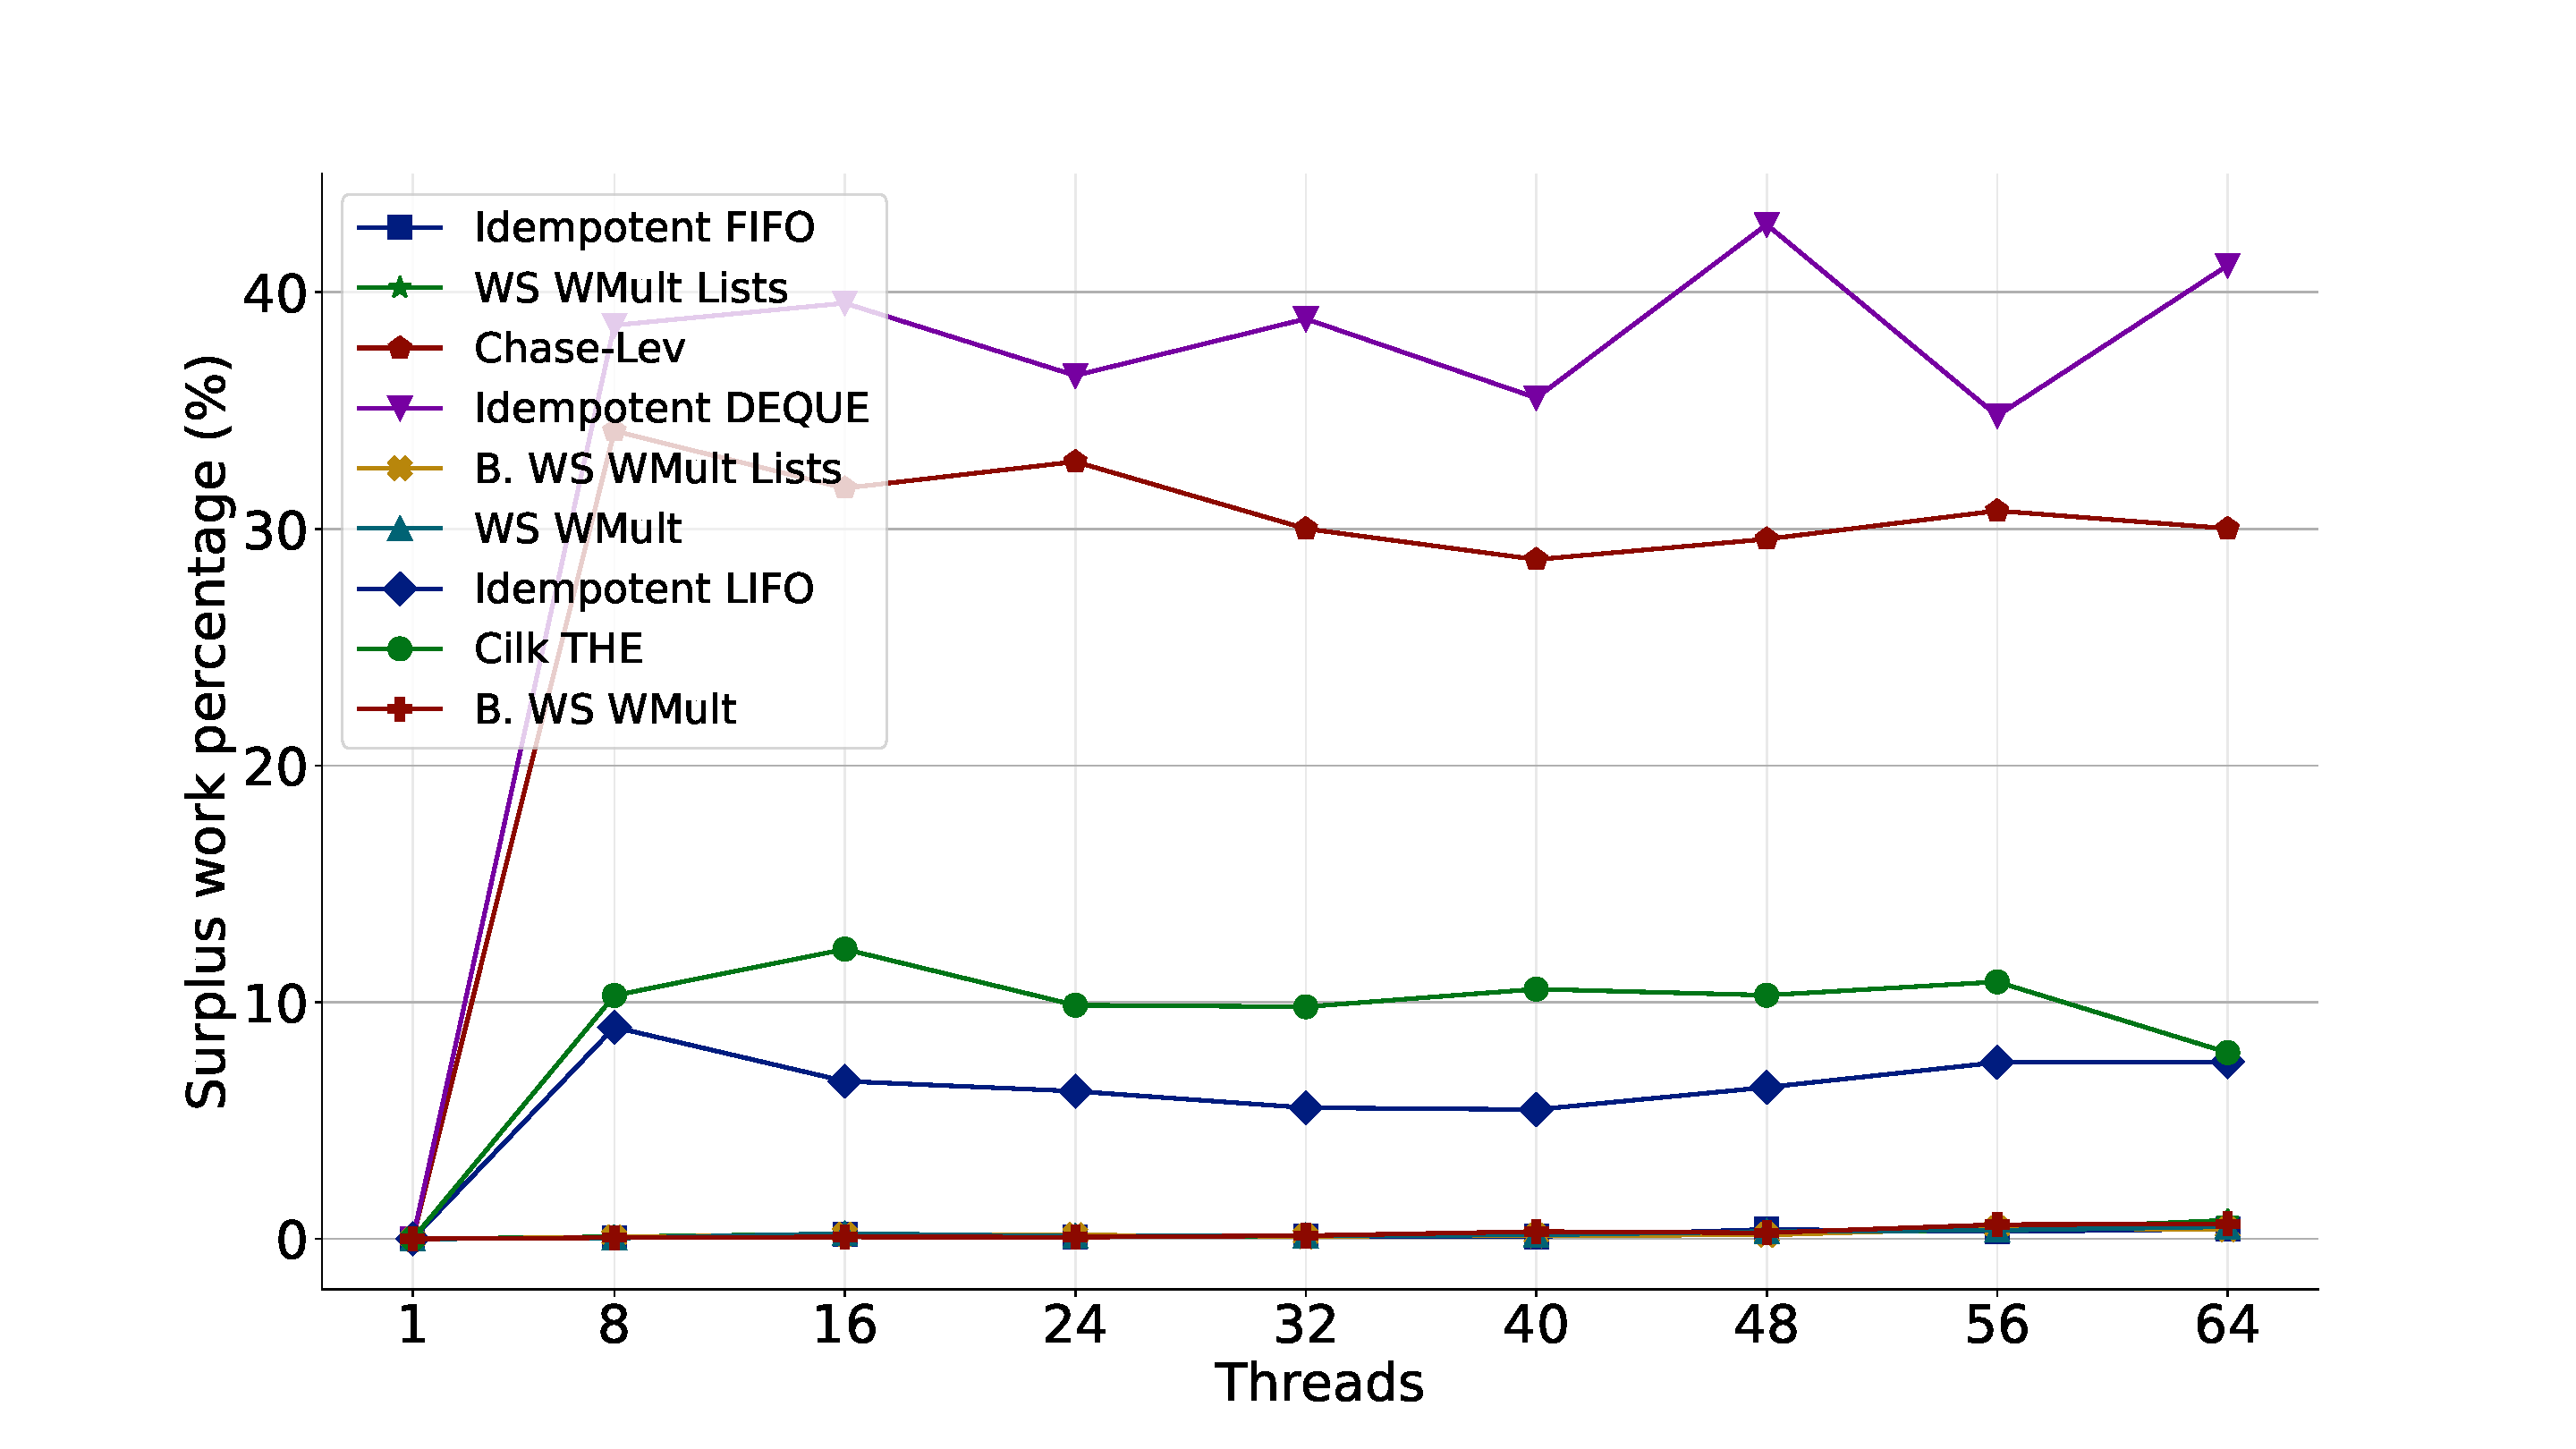
\includegraphics[width=0.48\textwidth]{contents/backmatter/evaluation/mult-torus_3d_directed_256.pdf}
  }
  \subfloat[\label{fig:surplustorus3ddirected-appx:1000000}Surplus work: Directed Torus 3D. Initial size of 1,000,000 items]{
    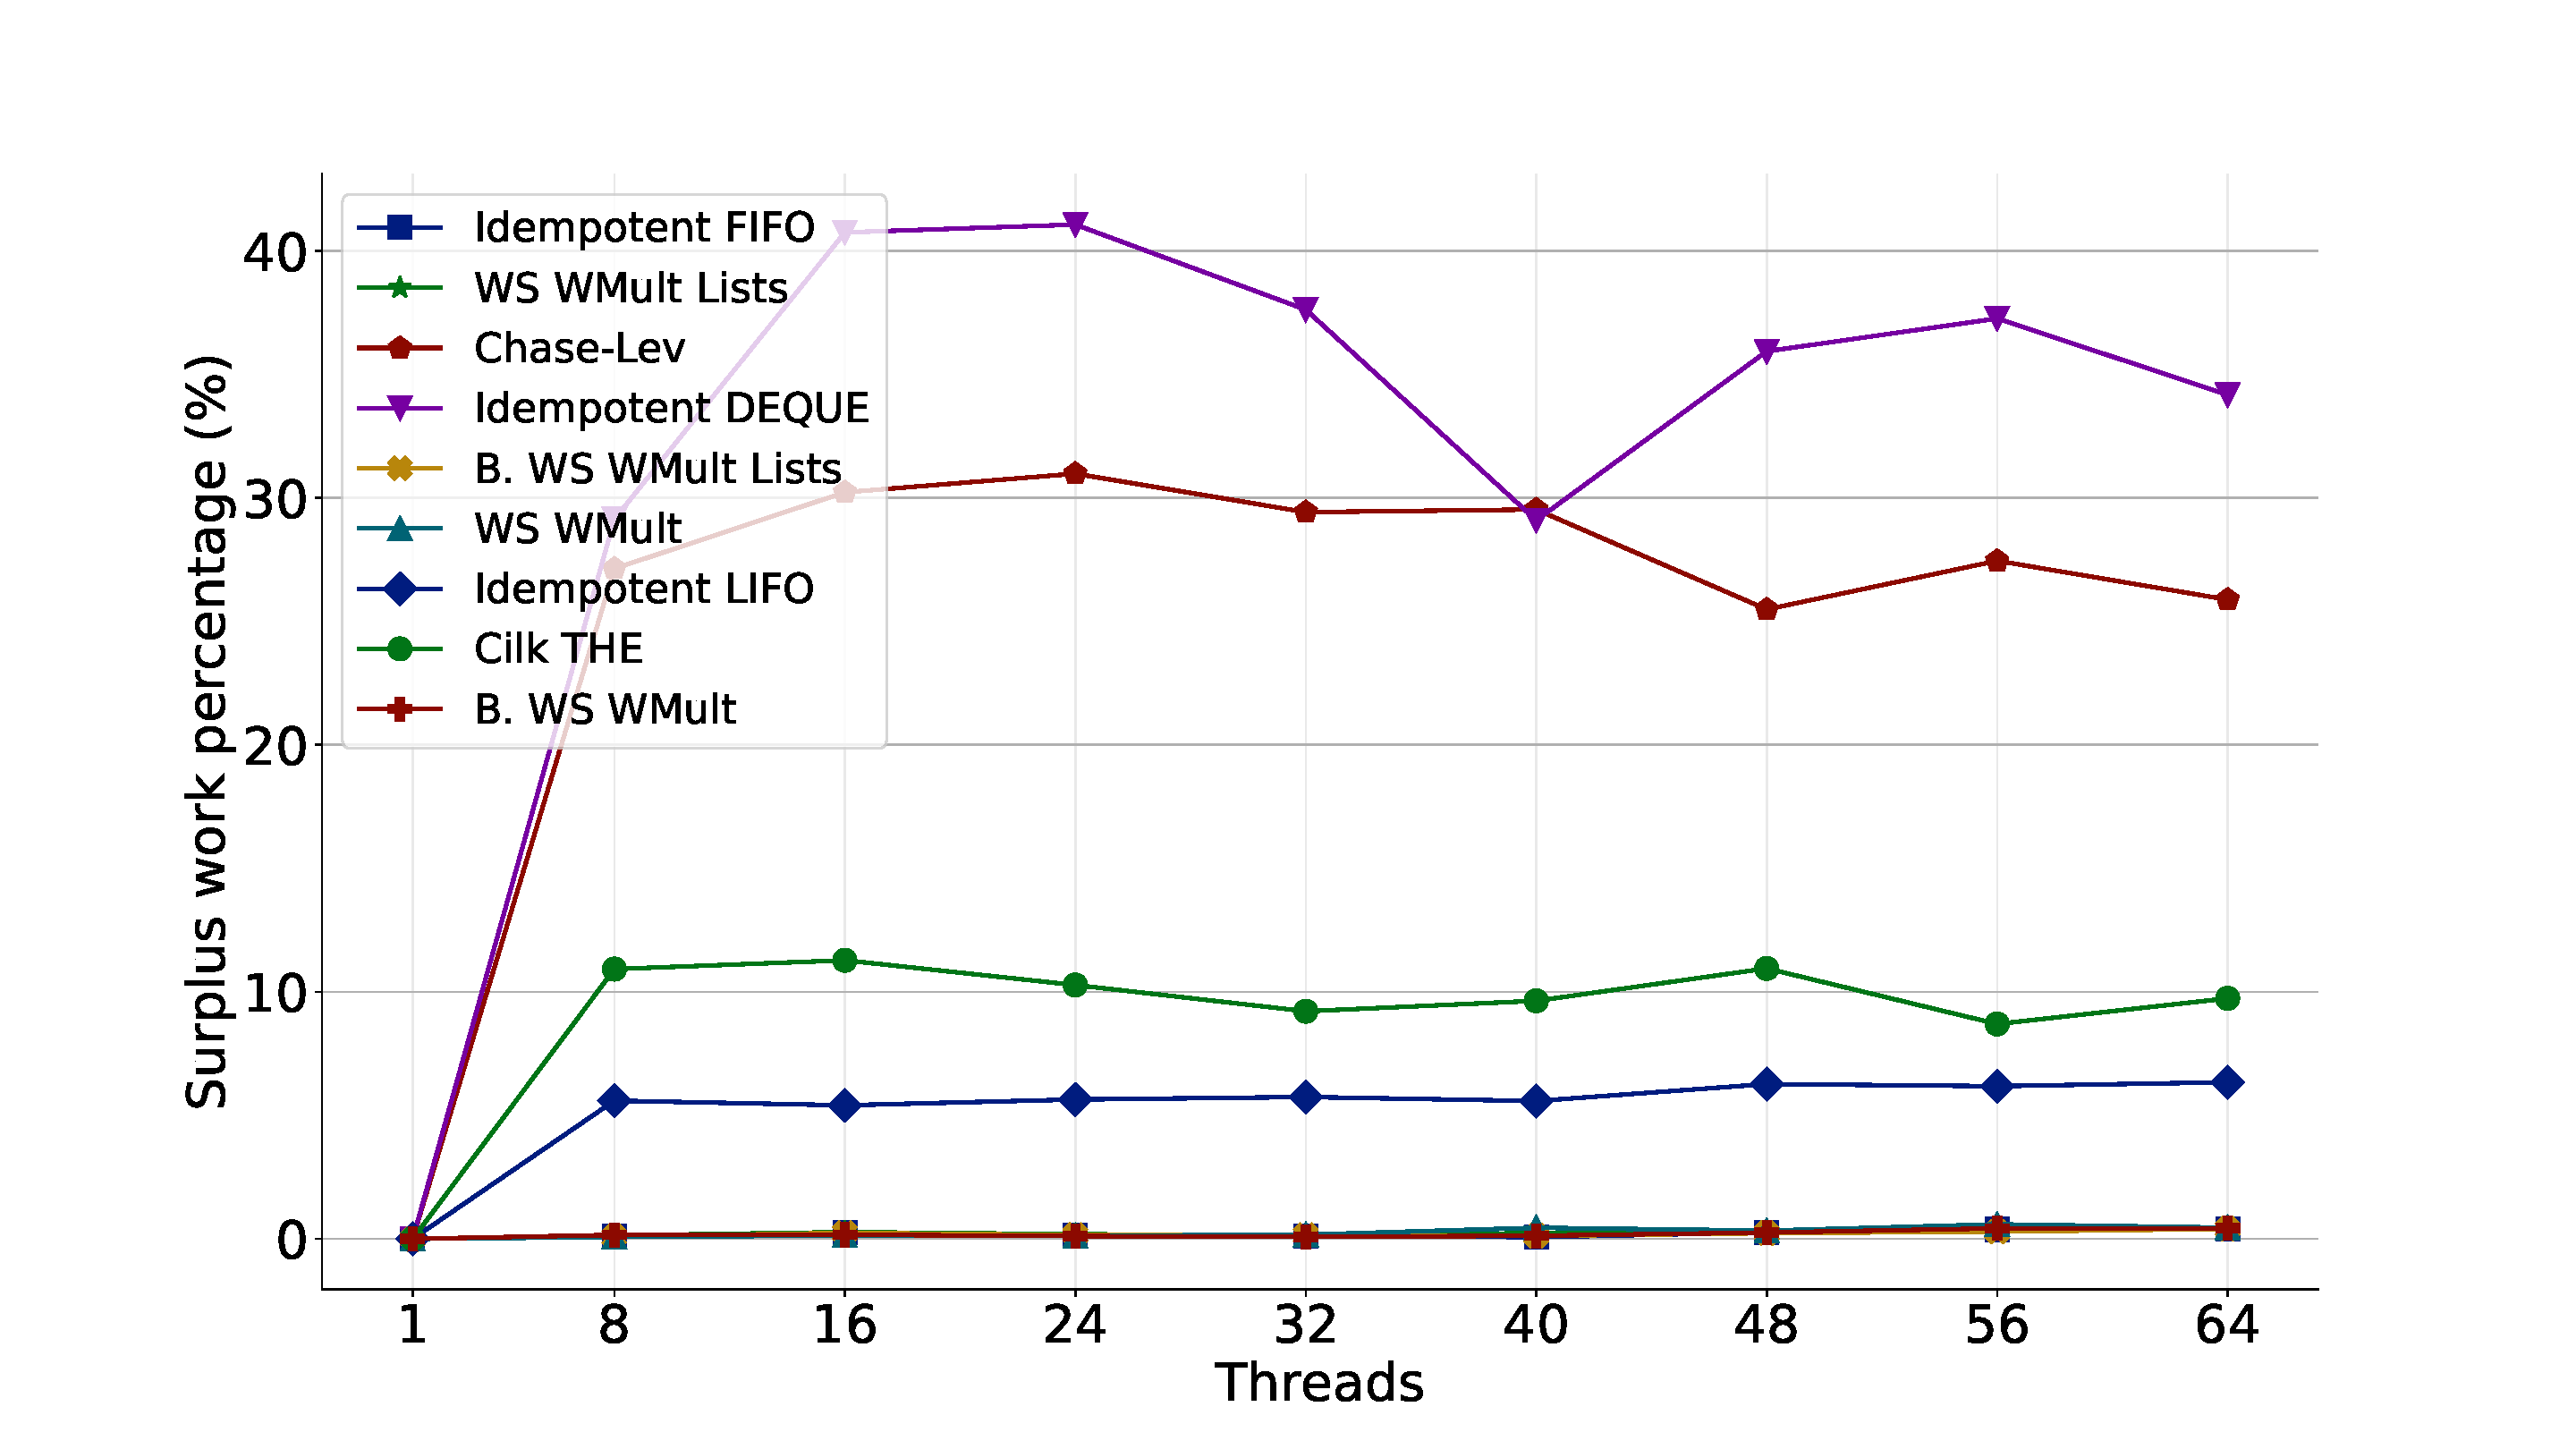
\includegraphics[width=0.48\textwidth]{contents/backmatter/evaluation/mult-torus_3d_directed_1m.pdf}
  }

  \subfloat[\label{fig:surplustorus3dundirected-appx:256}Surplus work: Undirected Torus 3D. Initial size of 256 items]{
    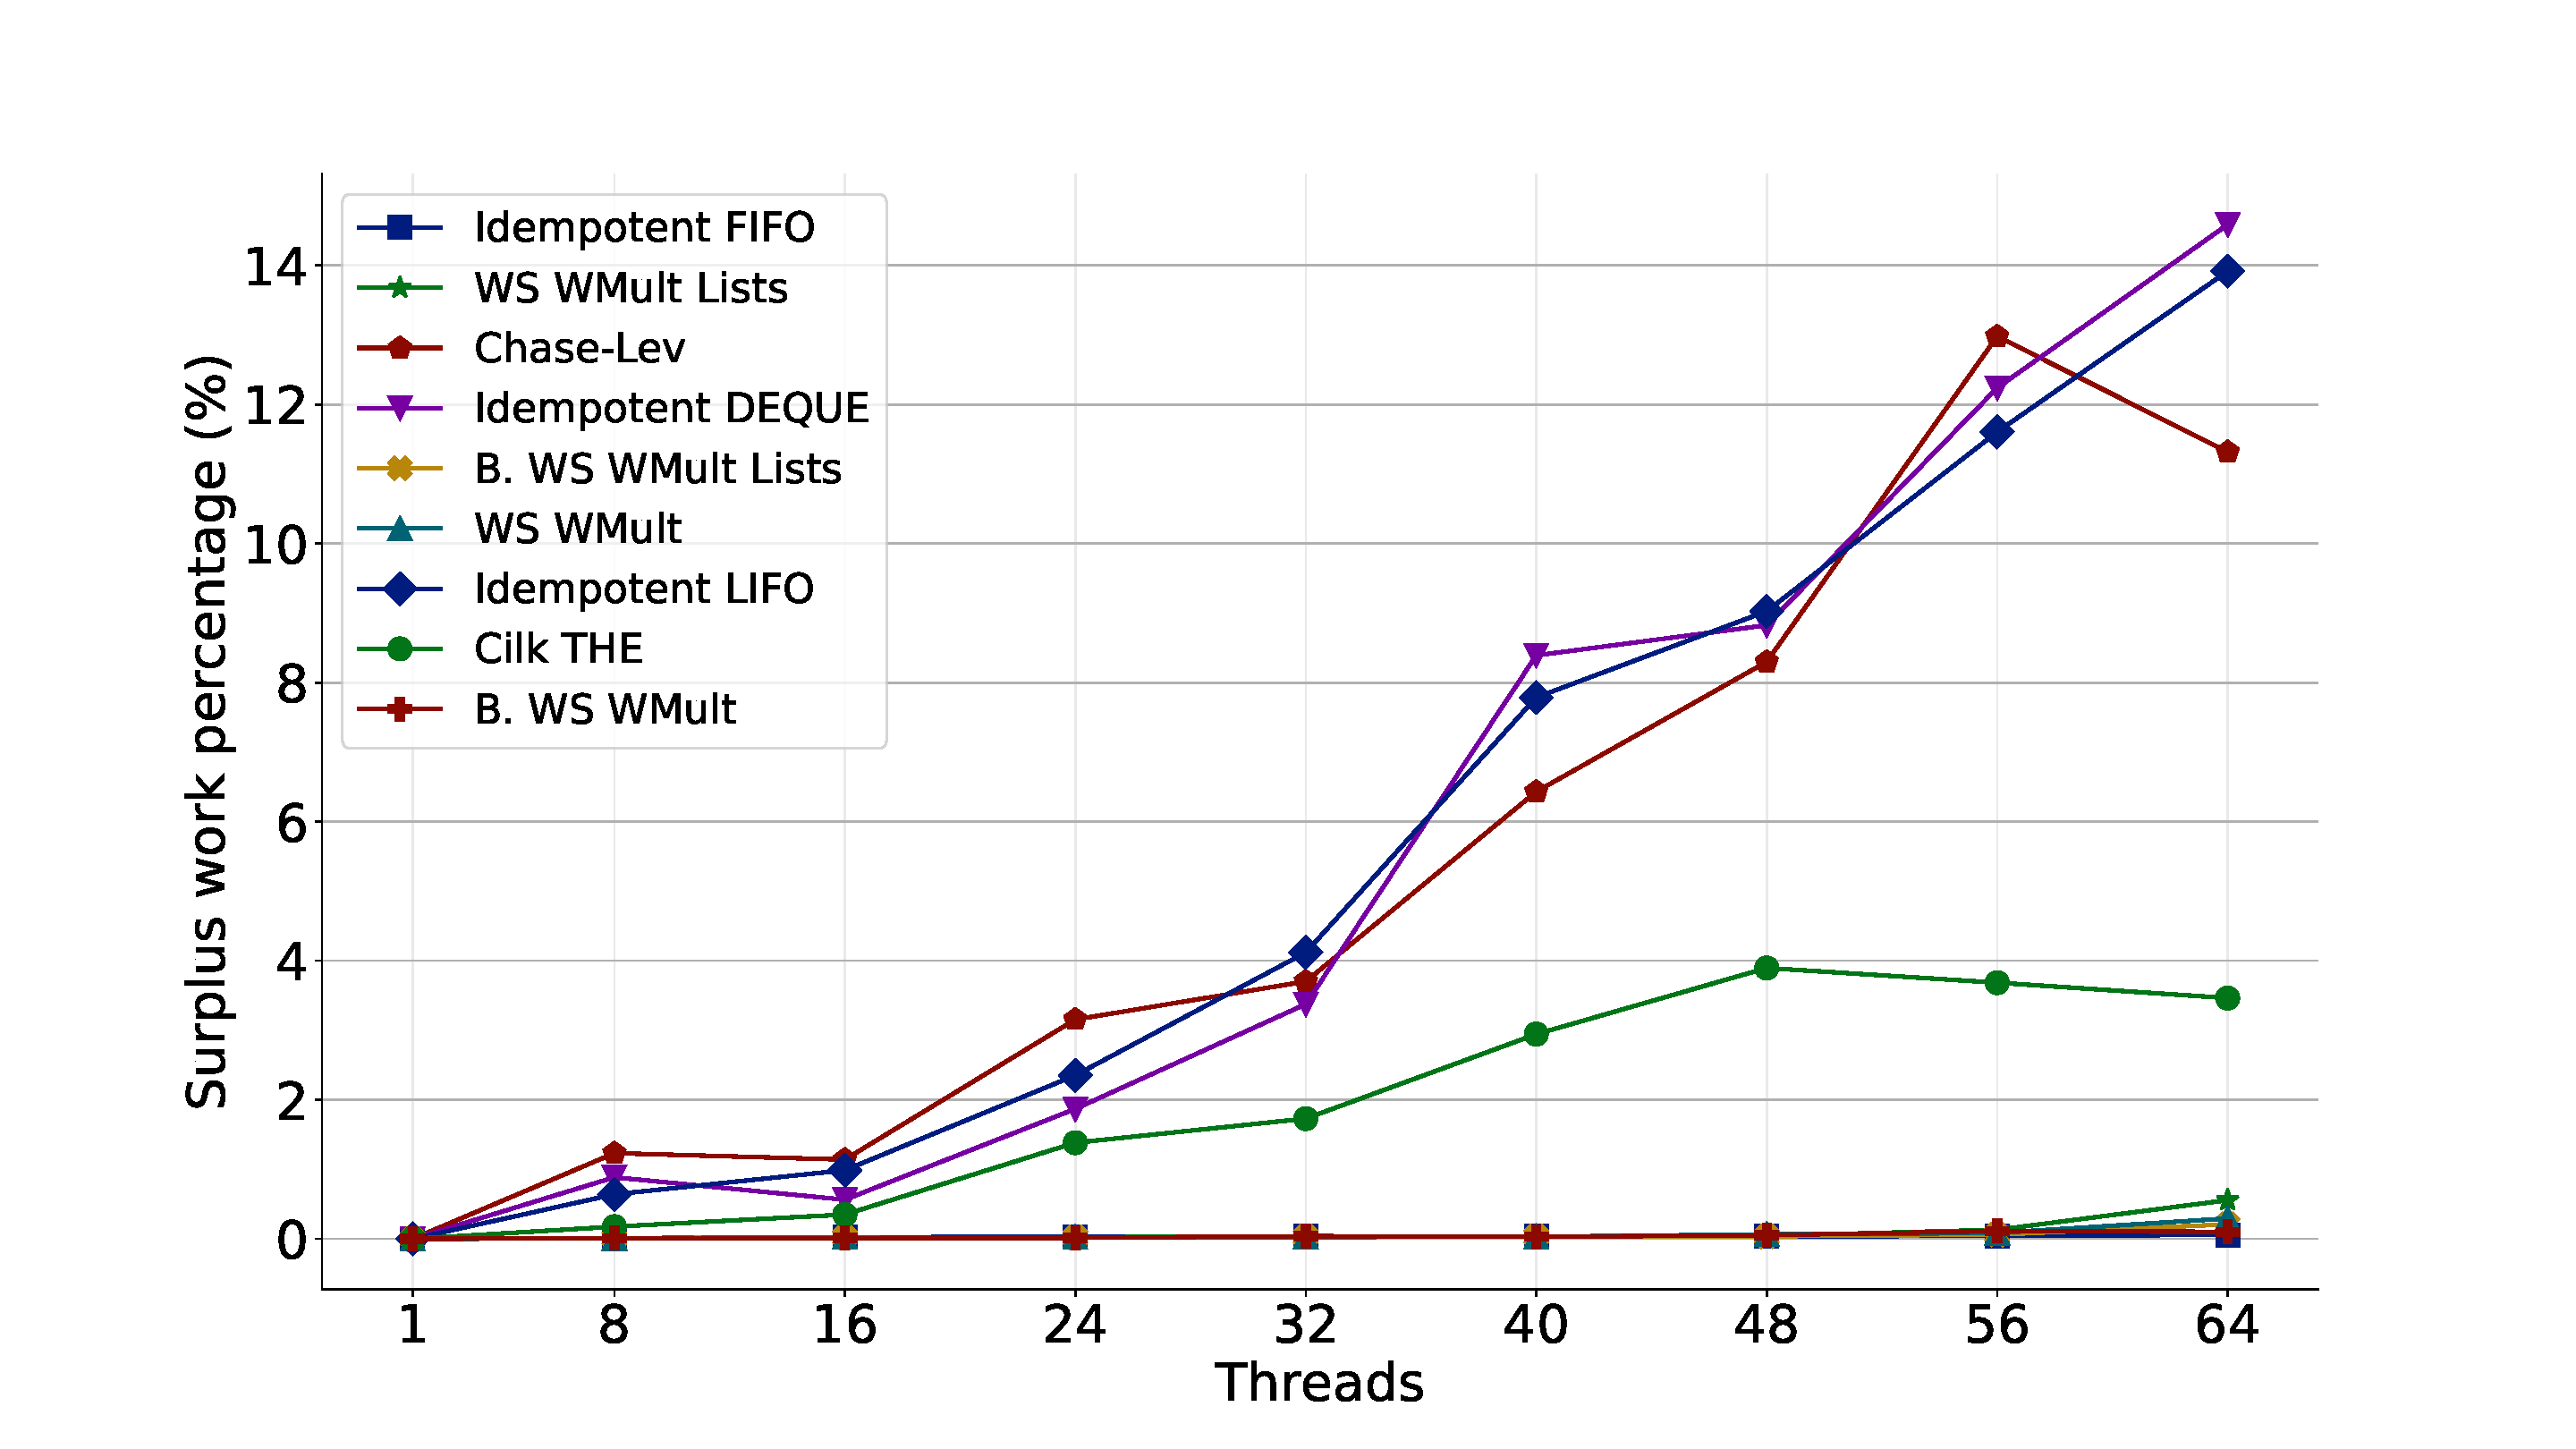
\includegraphics[width=0.48\textwidth]{contents/backmatter/evaluation/mult-torus_3d_undirected_256.pdf}
  }
  \subfloat[\label{fig:surplustorus3dundirected:1000000}Surplus work: Undirected Torus 3D. Initial size of 1,000,000 items]{
    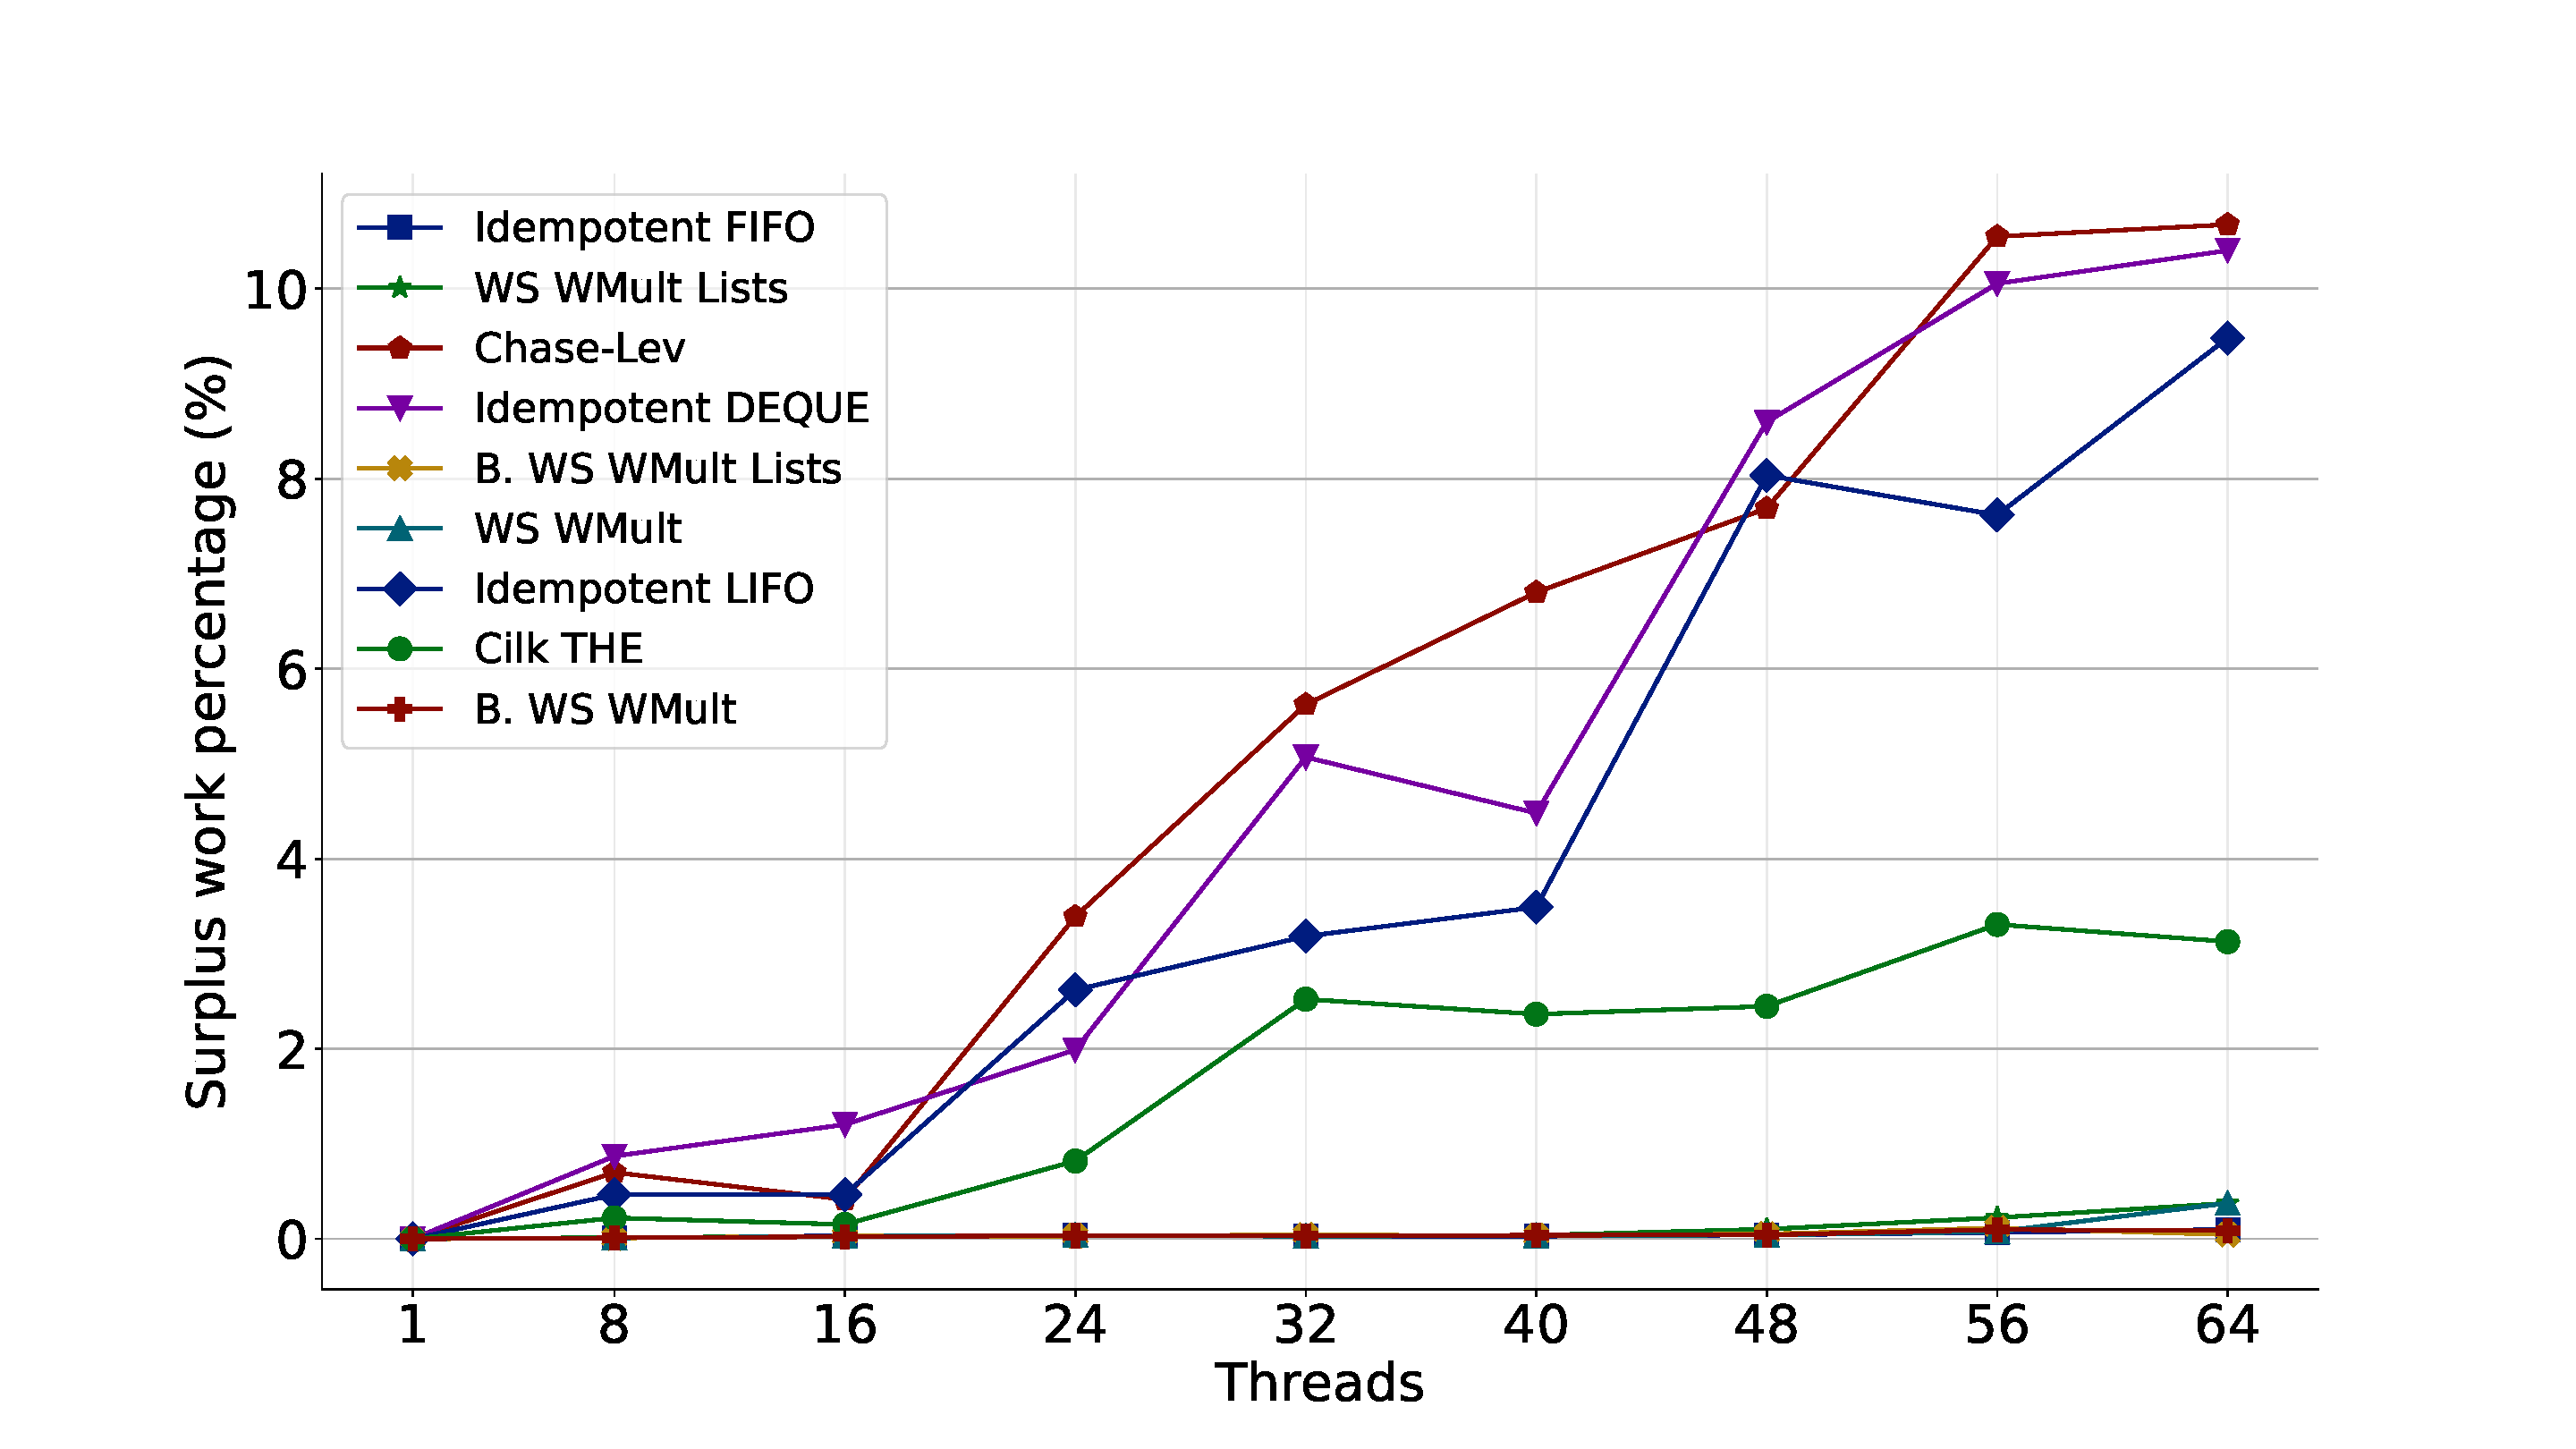
\includegraphics[width=0.48\textwidth]{contents/backmatter/evaluation/mult-torus_3d_undirected_1m.pdf}
  }

  \caption{\label{fig:surplusgraphapplicationtorus3d} Surplus work
    (percentage) of the experiments.  Surplus work: the difference
    between the total number of \Puts and the number of puts in
    sequential executions (i.e., $1,000,000$).}
\end{figure}

\begin{figure}[!ht]
  \subfloat[\label{fig:exec-surplustorus3ddirected-appx:256}Executed surplus work: Directed Torus 3D. Initial size of 256 items]{
    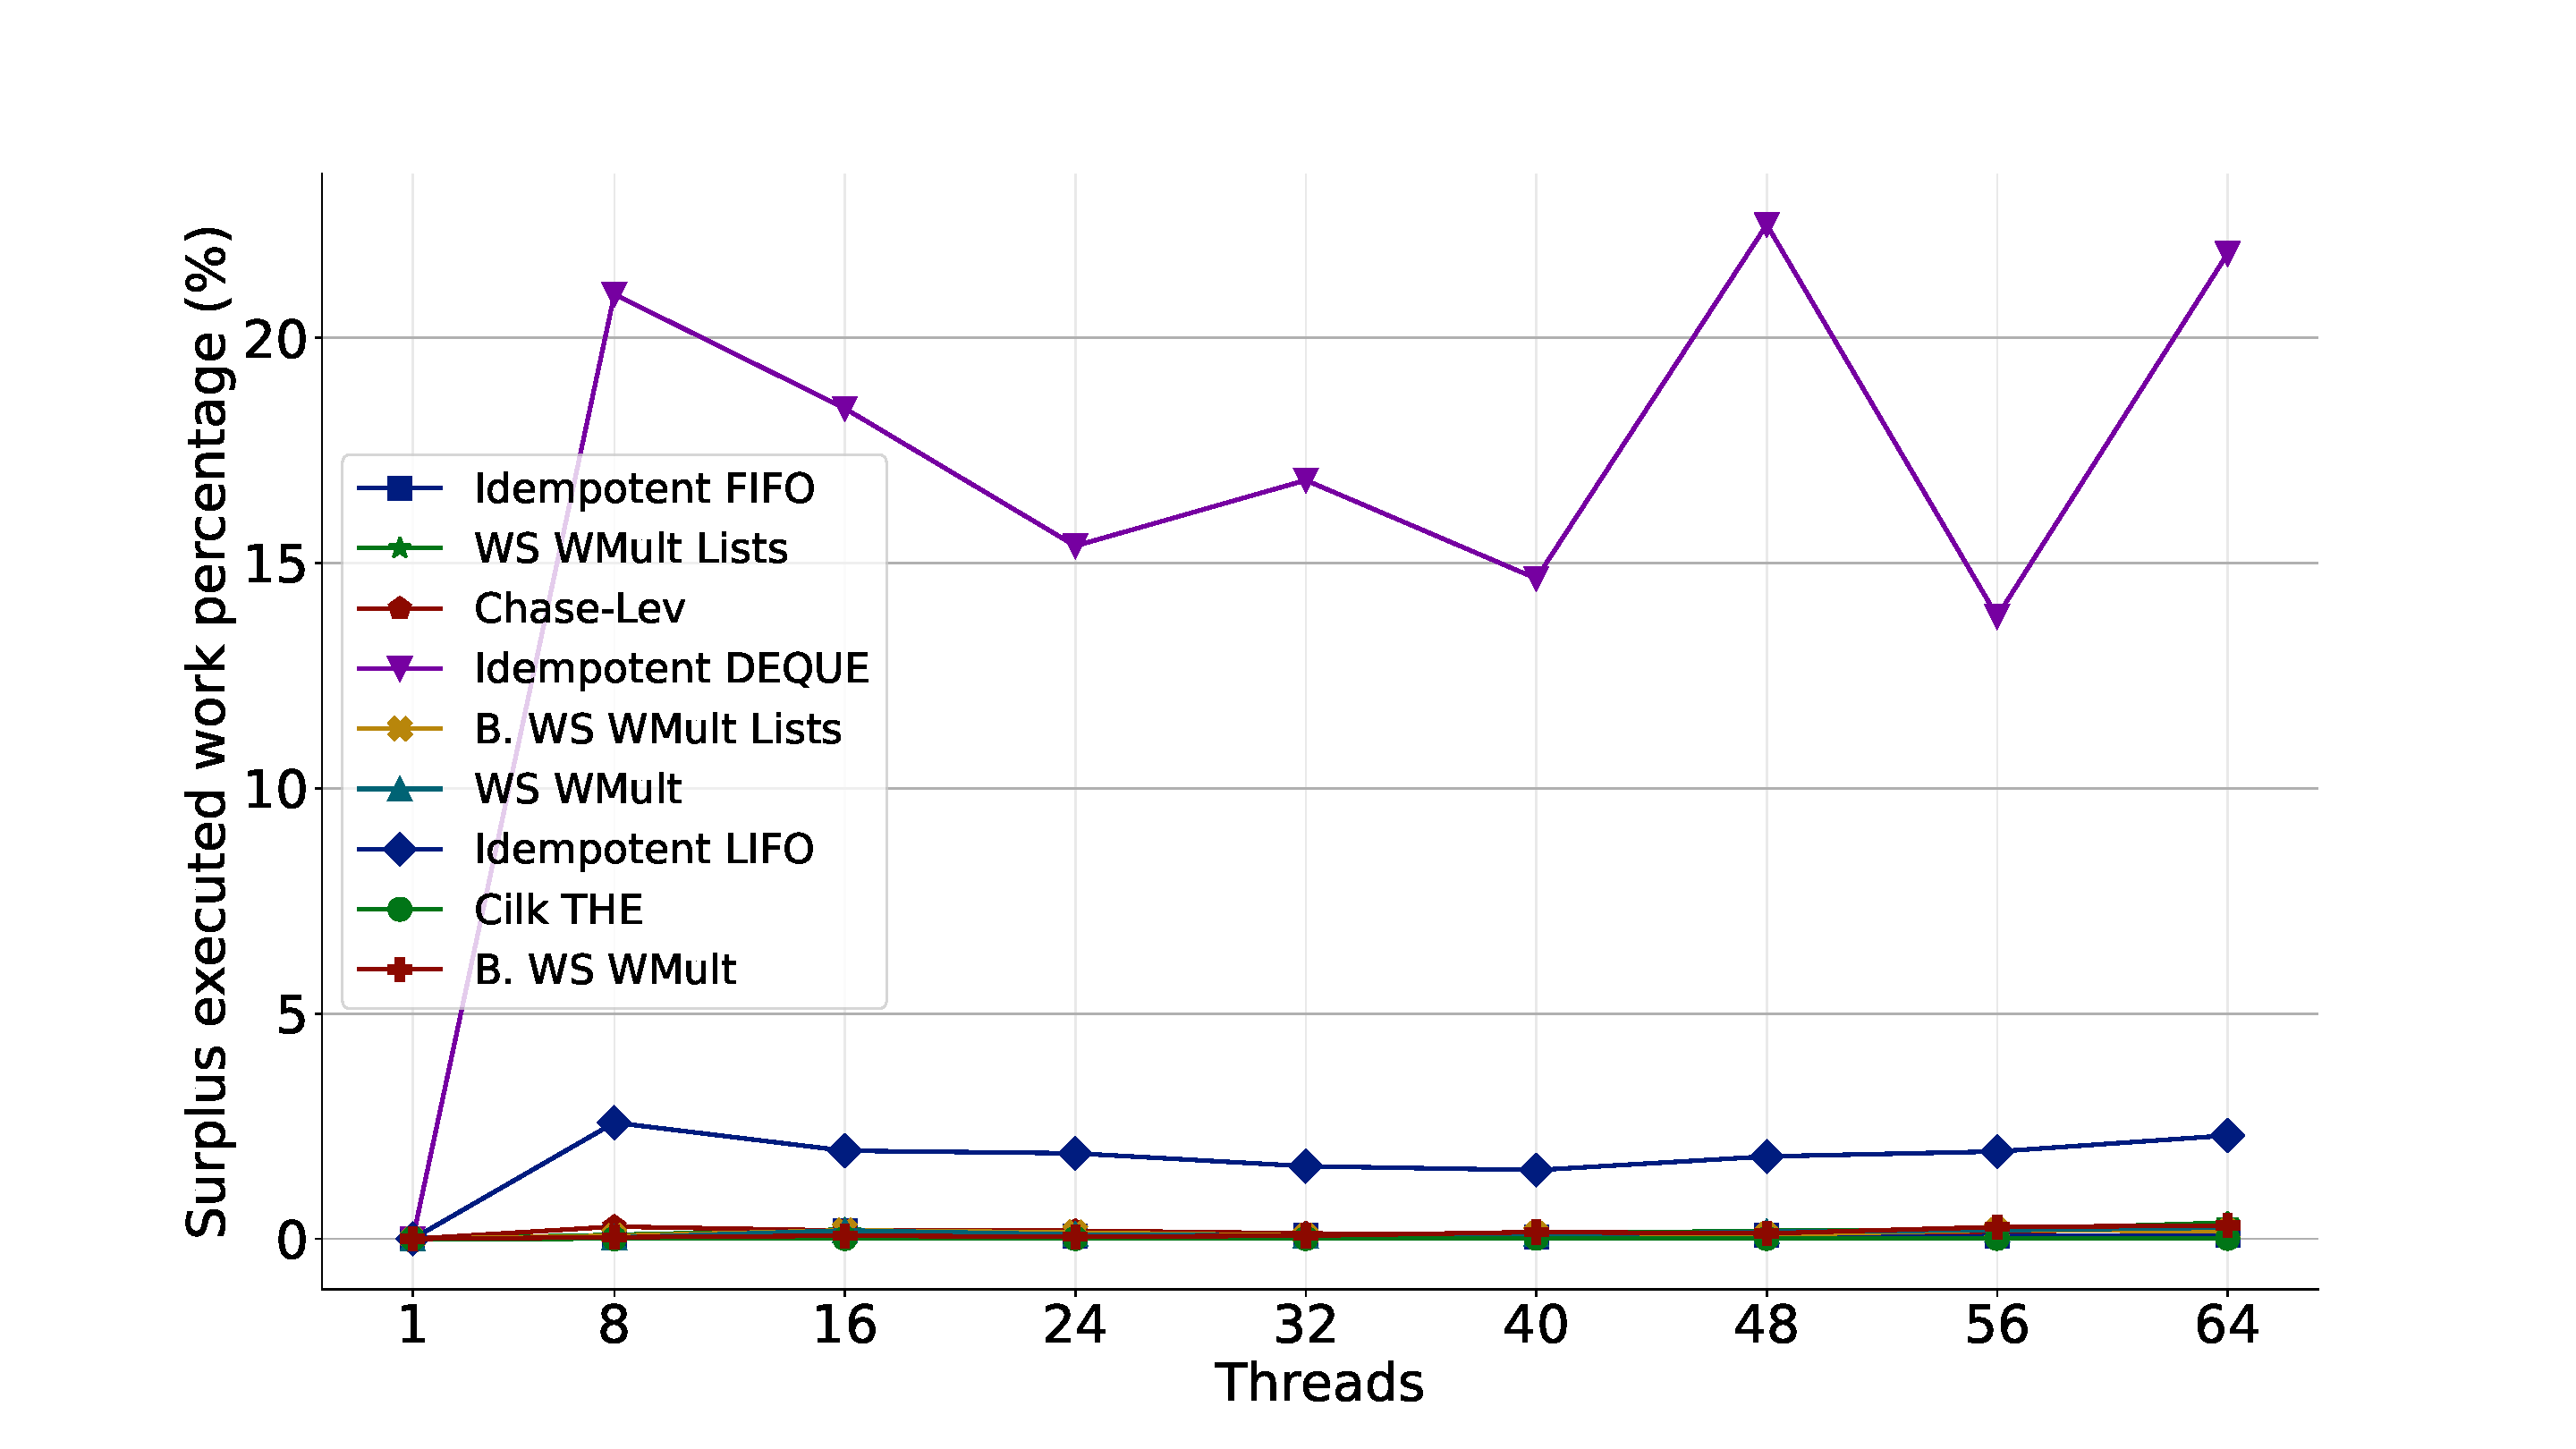
\includegraphics[width=0.48\textwidth]{contents/backmatter/evaluation/mult-exec-torus_3d_directed_256.pdf}
  }
  \subfloat[\label{fig:exec-surplustorus3ddirected-appx:1000000}Executed
  surplus work: Directed Torus 3D. Initial size of 1,000,000 items]{
    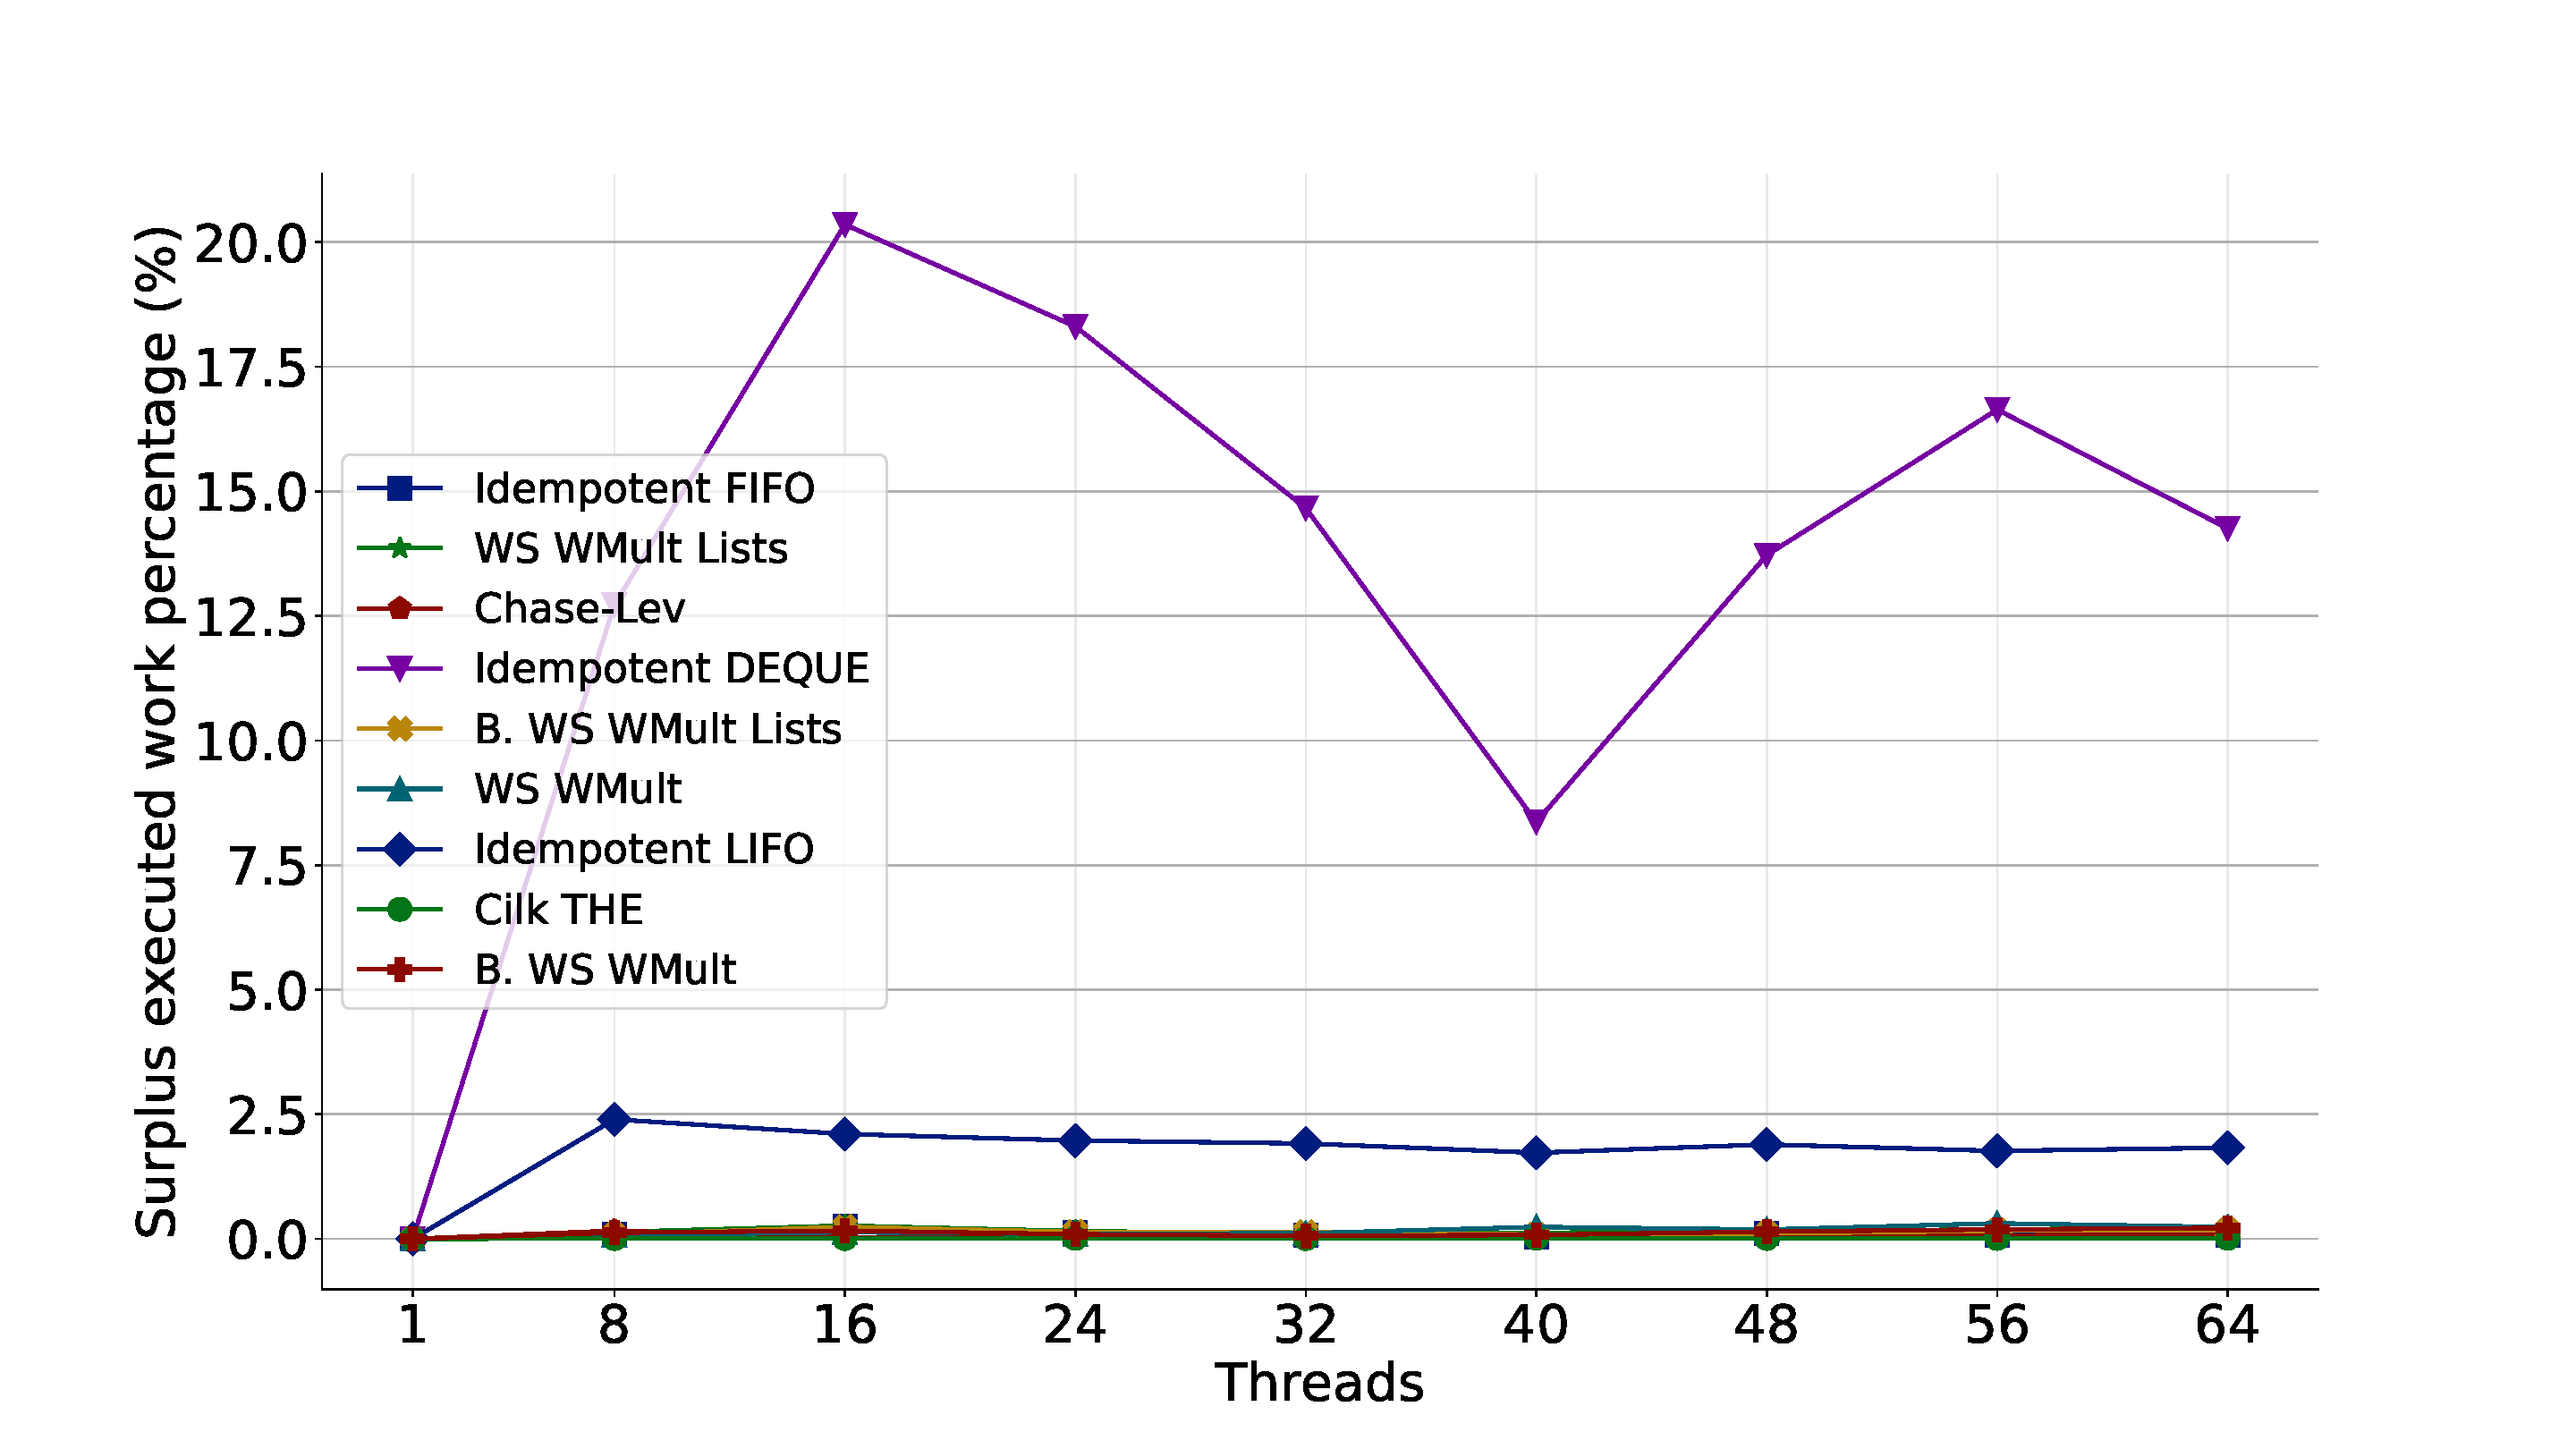
\includegraphics[width=0.48\textwidth]{contents/backmatter/evaluation/mult-exec-torus_3d_directed_1m.pdf}
  }

  \subfloat[\label{fig:exec-surplustorus3dundirected-appx:256}Executed
  surplus work: Undirected Torus 3D. Initial size of 256 items]{
    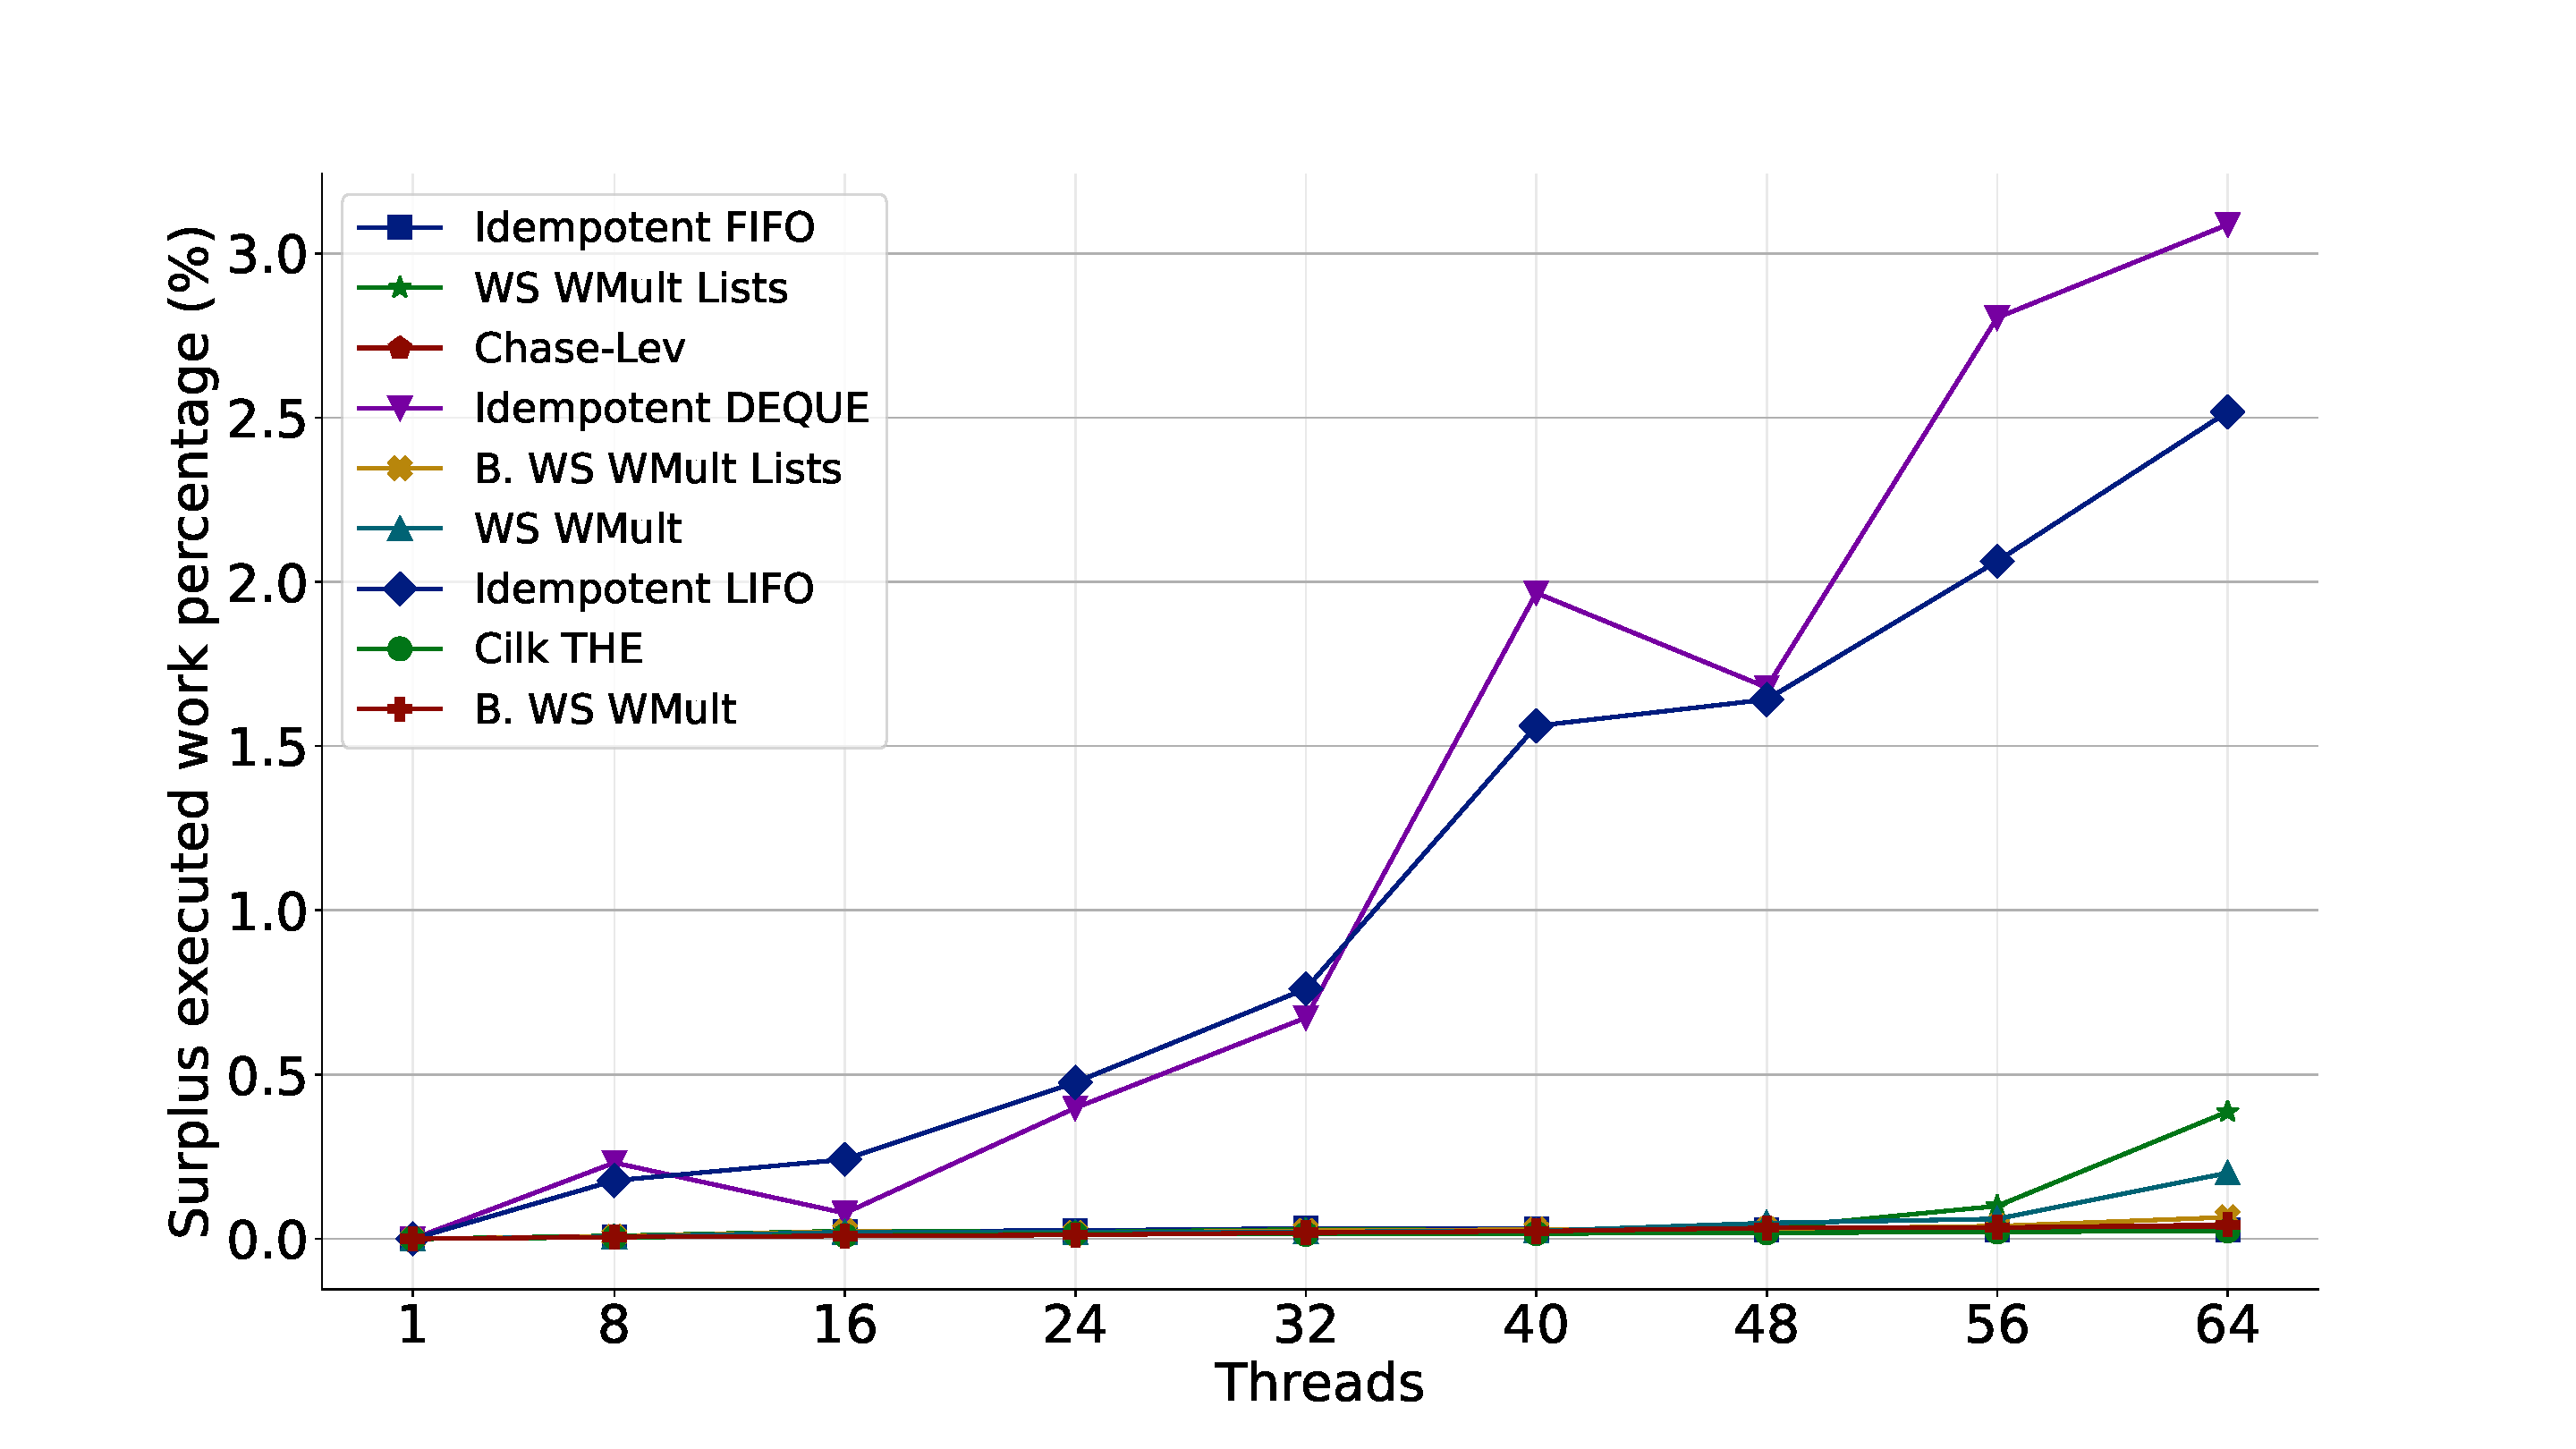
\includegraphics[width=0.48\textwidth]{contents/backmatter/evaluation/mult-exec-torus_3d_undirected_256.pdf}
  }
  \subfloat[\label{fig:exec-surplustorus3dundirected:1000000}Executed surplus work: Undirected Torus 3D. Initial size of 1,000,000 items]{
    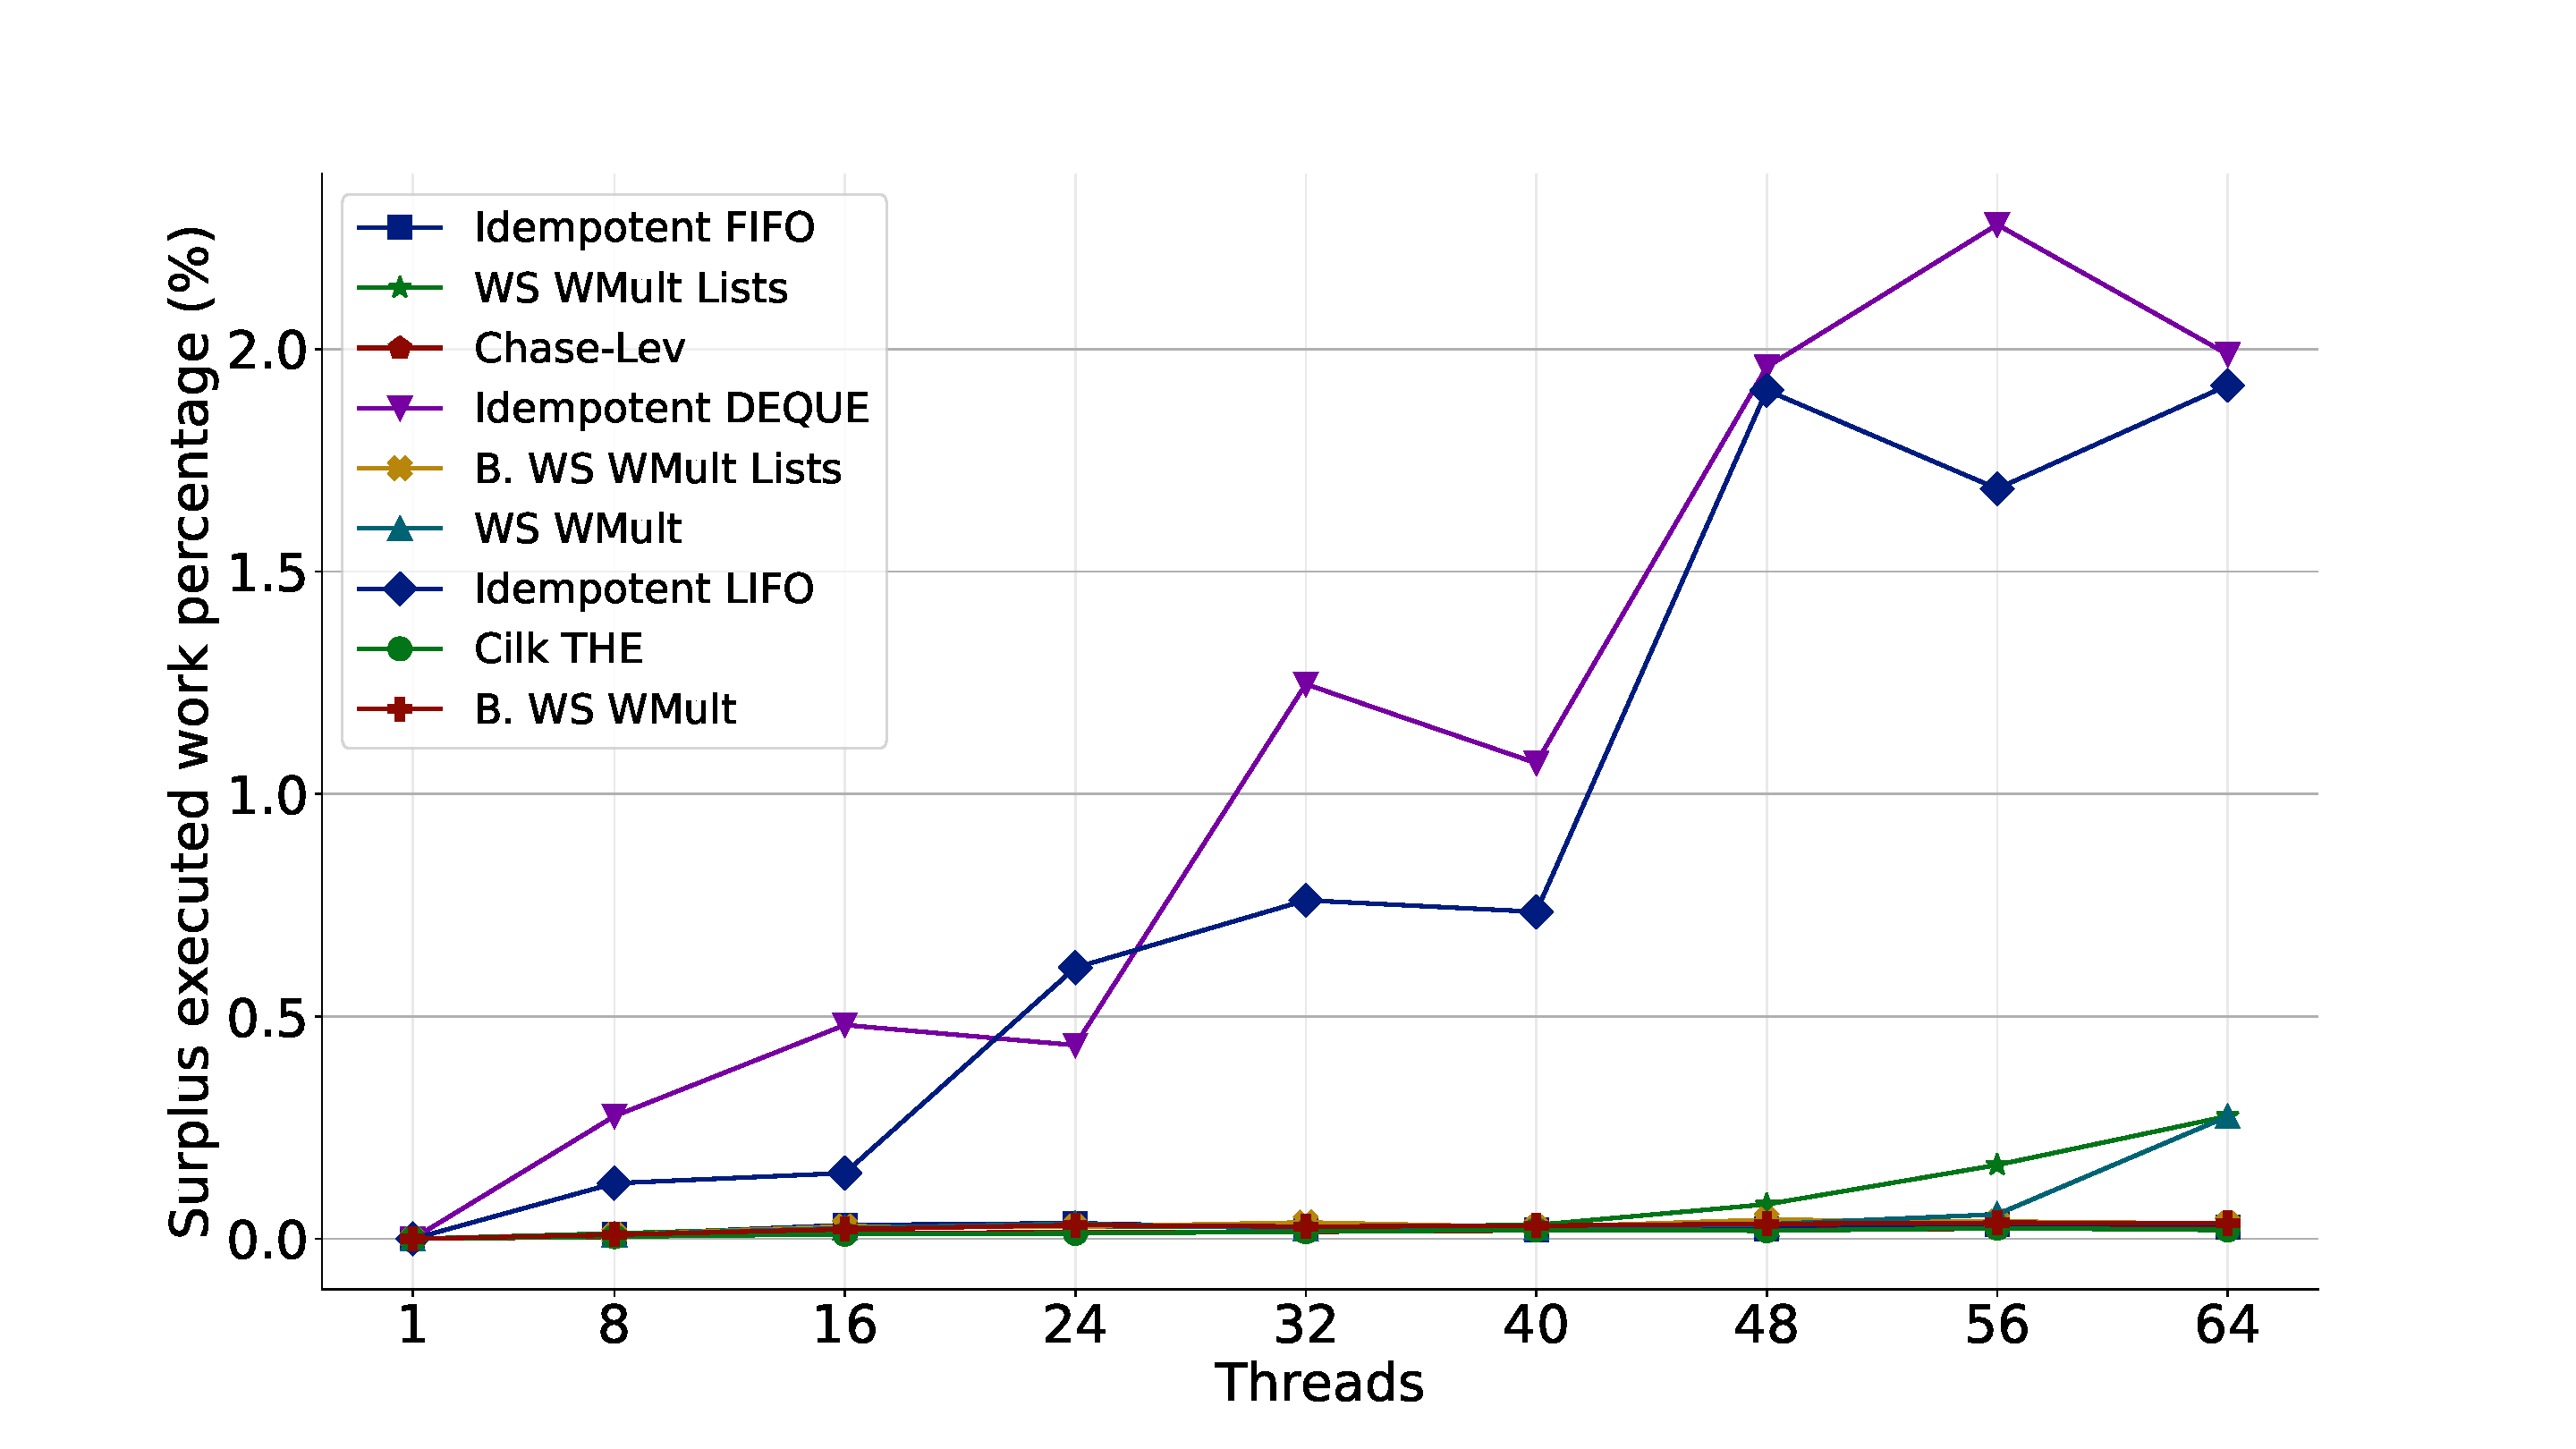
\includegraphics[width=0.48\textwidth]{contents/backmatter/evaluation/mult-exec-torus_3d_undirected_1m.pdf}
  }

  \caption{\label{fig:exec-surplusgraphapplicationtorus3d} Executed
    surplus work (percentage) of the experiments.  Surplus work: the
    difference between the total number of \Takes and the number of
    takes in sequential executions (i.e., $1,000,000$).}
\end{figure}

\clearpage{}

\subsubsection{Directed Torus 3D 40\%. Initial size of 256 items.}
\begin{table}[!ht]
\centering
\resizebox{\textwidth}{!}{\begin{tabular}{lrrrrrrrrrrrrrrr}
\toprule
\textbf{Algorithm} & \multicolumn{5}{l}{Chase-Lev} & \multicolumn{5}{l}{Cilk THE} & \multicolumn{5}{l}{Idempotent LIFO} \\
\textbf{Operation} &       Puts &      Takes & Difference (\%) & Surplus (\%) & Executed Surplus (\%) &       Puts &      Takes & Difference (\%) & Surplus (\%) & Executed Surplus (\%) &            Puts &      Takes & Difference (\%) & Surplus (\%) & Executed Surplus (\%) \\
\textbf{Processes} & \multicolumn{4}{l}{} & \multicolumn{4}{l}{} & \multicolumn{4}{l}{}\\ \midrule
\textbf{1 } & 1000000.00 & 1000000.00 &           0.00 &        0.00 &                 0.00 & 1000000.00 & 1000000.00 &           0.00 &        0.00 &                 0.00 &      1000000.00 & 1000000.00 &           0.00 &        0.00 &                 0.00 \\
\textbf{8 } & 1005449.60 & 1000025.40 &           0.54 &        0.54 &                 0.00 & 1003531.00 & 1000011.60 &           0.35 &        0.35 &                 0.00 &      1007831.60 & 1003007.60 &           0.48 &        0.78 &                 0.30 \\
\textbf{16} & 1007845.00 & 1000040.80 &           0.77 &        0.78 &                 0.00 & 1003157.80 & 1000021.20 &           0.31 &        0.31 &                 0.00 &      1007907.00 & 1002678.20 &           0.52 &        0.78 &                 0.27 \\
\textbf{24} & 1010827.80 & 1000051.00 &           1.07 &        1.07 &                 0.01 & 1014180.00 & 1000052.40 &           1.39 &        1.40 &                 0.01 &      1012551.00 & 1003577.60 &           0.89 &        1.24 &                 0.36 \\
\textbf{28} & 1018479.60 & 1000072.80 &           1.81 &        1.81 &                 0.01 & 1009475.60 & 1000041.40 &           0.93 &        0.94 &                 0.00 &      1025882.20 & 1006902.20 &           1.85 &        2.52 &                 0.69 \\
\textbf{32} & 1020975.20 & 1000083.40 &           2.05 &        2.05 &                 0.01 & 1018990.80 & 1000064.00 &           1.86 &        1.86 &                 0.01 &      1031138.00 & 1009279.60 &           2.12 &        3.02 &                 0.92 \\
\textbf{40} & 1034711.20 & 1000118.00 &           3.34 &        3.35 &                 0.01 & 1020566.60 & 1000070.60 &           2.01 &        2.02 &                 0.01 &      1050068.40 & 1012530.20 &           3.57 &        4.77 &                 1.24 \\
\textbf{48} & 1057946.40 & 1000196.00 &           5.46 &        5.48 &                 0.02 & 1033972.80 & 1000102.40 &           3.28 &        3.29 &                 0.01 &      1068848.60 & 1016887.80 &           4.86 &        6.44 &                 1.66 \\
\textbf{56} & 1068222.80 & 1000269.20 &           6.36 &        6.39 &                 0.03 & 1026236.60 & 1000101.20 &           2.55 &        2.56 &                 0.01 &      1072725.20 & 1018435.00 &           5.06 &        6.78 &                 1.81 \\
\textbf{64} & 1081135.20 & 1000354.40 &           7.47 &        7.50 &                 0.04 & 1034986.40 & 1000129.00 &           3.37 &        3.38 &                 0.01 &      1084878.80 & 1019539.00 &           6.02 &        7.82 &                 1.92 \\
\bottomrule
\end{tabular}}
\label{difference-Torus_3D_40_directed-256-CHASELEV-CILK-IDEMPOTENT_LIFO}
\caption{The number of puts and takes performed during the
    spanning tree experiment on a Torus 3D 40 directed graph with an initial size
    of 256 items is provided. The table presents data on the
    following algorithms: Chase-Lev, Cilk THE, and
    Idempotent LIFO. Furthermore, we present the percentage difference
    between the number of puts and takes for each available thread,
    relative to the total number of puts. Finally, also we show the
    "surplus" work, which is the difference of the total number of
    \Puts (Work to be scheduled) and the total number of \Puts in
    sequential executions (i.e., 1,000,000), and the "executed surplus
    work", which is the difference between the total number of \Takes
    (actual work executed) and the total of \Takes in sequential
    executions.}
\end{table}

\begin{table}[!ht]
\centering
\resizebox{\textwidth}{!}{\begin{tabular}{lrrrrrrrrrrrrrrr}
\toprule
\textbf{Algorithm} & \multicolumn{5}{l}{Idempotent DEQUE} & \multicolumn{5}{l}{Idempotent FIFO} & \multicolumn{5}{l}{WS WMult} \\
\textbf{Operation} &             Puts &      Takes & Difference (\%) & Surplus (\%) & Executed Surplus (\%) &            Puts &      Takes & Difference (\%) & Surplus (\%) & Executed Surplus (\%) &       Puts &      Takes & Difference (\%) & Surplus (\%) & Executed Surplus (\%) \\
\textbf{Processes} & \multicolumn{4}{l}{} & \multicolumn{4}{l}{} & \multicolumn{4}{l}{}\\ \midrule
\textbf{1 } &       1000000.00 & 1000000.00 &           0.00 &        0.00 &                 0.00 &      1000000.00 & 1000000.00 &           0.00 &        0.00 &                 0.00 & 1000000.00 & 1000000.00 &           0.00 &        0.00 &                 0.00 \\
\textbf{8 } &       1008481.80 & 1003449.40 &           0.50 &        0.84 &                 0.34 &      1000128.80 & 1000055.00 &           0.01 &        0.01 &                 0.01 & 1000526.80 & 1000219.80 &           0.03 &        0.05 &                 0.02 \\
\textbf{16} &       1005470.20 & 1001761.00 &           0.37 &        0.54 &                 0.18 &      1000658.00 & 1000200.00 &           0.05 &        0.07 &                 0.02 & 1000935.00 & 1000436.80 &           0.05 &        0.09 &                 0.04 \\
\textbf{24} &       1009159.80 & 1002624.60 &           0.65 &        0.91 &                 0.26 &      1000920.00 & 1000149.80 &           0.08 &        0.09 &                 0.01 & 1003026.40 & 1001321.00 &           0.17 &        0.30 &                 0.13 \\
\textbf{28} &       1015154.40 & 1003866.60 &           1.11 &        1.49 &                 0.39 &      1001958.60 & 1000274.20 &           0.17 &        0.20 &                 0.03 & 1002323.40 & 1000898.80 &           0.14 &        0.23 &                 0.09 \\
\textbf{32} &       1017233.80 & 1004198.20 &           1.28 &        1.69 &                 0.42 &      1001449.80 & 1000200.40 &           0.12 &        0.14 &                 0.02 & 1002768.00 & 1001051.00 &           0.17 &        0.28 &                 0.10 \\
\textbf{40} &       1046653.80 & 1011064.20 &           3.40 &        4.46 &                 1.09 &      1003686.00 & 1000461.20 &           0.32 &        0.37 &                 0.05 & 1004101.00 & 1001486.00 &           0.26 &        0.41 &                 0.15 \\
\textbf{48} &       1068845.40 & 1016652.60 &           4.88 &        6.44 &                 1.64 &      1005327.00 & 1000561.80 &           0.47 &        0.53 &                 0.06 & 1007847.20 & 1003027.40 &           0.48 &        0.78 &                 0.30 \\
\textbf{56} &       1070162.00 & 1013574.00 &           5.29 &        6.56 &                 1.34 &      1008234.00 & 1000919.00 &           0.73 &        0.82 &                 0.09 & 1009025.80 & 1002972.00 &           0.60 &        0.89 &                 0.30 \\
\textbf{64} &       1105482.20 & 1023885.60 &           7.38 &        9.54 &                 2.33 &      1006061.80 & 1000680.80 &           0.53 &        0.60 &                 0.07 & 1010481.40 & 1003566.20 &           0.68 &        1.04 &                 0.36 \\
\bottomrule
\end{tabular}}
\label{difference-Torus_3D_40_directed-256-IDEMPOTENT_DEQUE-IDEMPOTENT_FIFO-WS_NC_MULT_OPT}
\caption{The number of puts and takes performed during the
    spanning tree experiment on a Torus 3D 40 directed graph with an initial size
    of 256 items is provided. The table presents data on the
    following algorithms: Idempotent DEQUE, Idempotent FIFO, and
    WS WMult. Furthermore, we present the percentage difference
    between the number of puts and takes for each available thread,
    relative to the total number of puts. Finally, also we show the
    "surplus" work, which is the difference of the total number of
    \Puts (Work to be scheduled) and the total number of \Puts in
    sequential executions (i.e., 1,000,000), and the "executed surplus
    work", which is the difference between the total number of \Takes
    (actual work executed) and the total of \Takes in sequential
    executions.}
\end{table}

\begin{table}[!ht]
\centering
\resizebox{\textwidth}{!}{\begin{tabular}{lrrrrrrrrrrrrrrr}
\toprule
\textbf{Algorithm} & \multicolumn{5}{l}{B. WS WMult} & \multicolumn{5}{l}{WS WMult Lists} & \multicolumn{5}{l}{B. WS WMult Lists} \\
\textbf{Operation} &        Puts &      Takes & Difference (\%) & Surplus (\%) & Executed Surplus (\%) &           Puts &      Takes & Difference (\%) & Surplus (\%) & Executed Surplus (\%) &              Puts &      Takes & Difference (\%) & Surplus (\%) & Executed Surplus (\%) \\
\textbf{Processes} & \multicolumn{4}{l}{} & \multicolumn{4}{l}{} & \multicolumn{4}{l}{}\\ \midrule
\textbf{1 } &  1000000.00 & 1000000.00 &           0.00 &        0.00 &                 0.00 &     1000000.00 & 1000000.00 &           0.00 &        0.00 &                 0.00 &        1000000.00 & 1000000.00 &           0.00 &        0.00 &                 0.00 \\
\textbf{8 } &  1001496.00 & 1000859.80 &           0.06 &        0.15 &                 0.09 &     1000215.20 & 1000154.00 &           0.01 &        0.02 &                 0.02 &        1000227.20 & 1000153.60 &           0.01 &        0.02 &                 0.02 \\
\textbf{16} &  1001202.00 & 1000555.00 &           0.06 &        0.12 &                 0.06 &     1000642.80 & 1000386.60 &           0.03 &        0.06 &                 0.04 &        1000830.00 & 1000488.00 &           0.03 &        0.08 &                 0.05 \\
\textbf{24} &  1001979.40 & 1000864.40 &           0.11 &        0.20 &                 0.09 &     1001499.00 & 1000901.80 &           0.06 &        0.15 &                 0.09 &        1001272.00 & 1000702.20 &           0.06 &        0.13 &                 0.07 \\
\textbf{28} &  1001512.20 & 1000549.40 &           0.10 &        0.15 &                 0.05 &     1001234.40 & 1000620.80 &           0.06 &        0.12 &                 0.06 &        1001945.00 & 1000943.60 &           0.10 &        0.19 &                 0.09 \\
\textbf{32} &  1003173.60 & 1001363.80 &           0.18 &        0.32 &                 0.14 &     1003907.80 & 1001866.60 &           0.20 &        0.39 &                 0.19 &        1002539.80 & 1001121.60 &           0.14 &        0.25 &                 0.11 \\
\textbf{40} &  1003953.20 & 1001584.80 &           0.24 &        0.39 &                 0.16 &     1003717.00 & 1001515.40 &           0.22 &        0.37 &                 0.15 &        1003422.80 & 1001369.80 &           0.20 &        0.34 &                 0.14 \\
\textbf{48} &  1004153.40 & 1001451.40 &           0.27 &        0.41 &                 0.14 &     1008118.80 & 1003261.20 &           0.48 &        0.81 &                 0.33 &        1003330.80 & 1001519.80 &           0.18 &        0.33 &                 0.15 \\
\textbf{56} &  1004527.40 & 1001453.00 &           0.31 &        0.45 &                 0.15 &     1008654.00 & 1003760.60 &           0.49 &        0.86 &                 0.37 &        1005827.80 & 1002499.80 &           0.33 &        0.58 &                 0.25 \\
\textbf{64} &  1008753.40 & 1003547.40 &           0.52 &        0.87 &                 0.35 &     1008999.20 & 1003677.20 &           0.53 &        0.89 &                 0.37 &        1007851.60 & 1002852.00 &           0.50 &        0.78 &                 0.28 \\
\bottomrule
\end{tabular}}
\label{difference-Torus_3D_40_directed-256-B_WS_NC_MULT_OPT-WS_NC_MULT_LA_OPT-B_WS_NC_MULT_LA_OPT}
\caption{The number of puts and takes performed during the
    spanning tree experiment on a Torus 3D 40 directed graph with an initial size
    of 256 items is provided. The table presents data on the
    following algorithms: B. WS WMult, WS WMult Lists, and
    B. WS WMult Lists. Furthermore, we present the percentage difference
    between the number of puts and takes for each available thread,
    relative to the total number of puts. Finally, also we show the
    "surplus" work, which is the difference of the total number of
    \Puts (Work to be scheduled) and the total number of \Puts in
    sequential executions (i.e., 1,000,000), and the "executed surplus
    work", which is the difference between the total number of \Takes
    (actual work executed) and the total of \Takes in sequential
    executions.}
\end{table}

\clearpage
\subsubsection{Directed Torus 3D 40\%. Initial size of  1,000,000 items.}
\begin{table}[!ht]
\centering
\resizebox{\textwidth}{!}{\begin{tabular}{lrrrrrrrrrrrrrrr}
\toprule
\textbf{Algorithm} & \multicolumn{5}{l}{Chase-Lev} & \multicolumn{5}{l}{Cilk THE} & \multicolumn{5}{l}{Idempotent LIFO} \\
\textbf{Operation} &       Puts &      Takes & Difference (\%) & Surplus (\%) & Executed Surplus (\%) &       Puts &      Takes & Difference (\%) & Surplus (\%) & Executed Surplus (\%) &            Puts &      Takes & Difference (\%) & Surplus (\%) & Executed Surplus (\%) \\
\textbf{Processes} & \multicolumn{4}{l}{} & \multicolumn{4}{l}{} & \multicolumn{4}{l}{}\\ \midrule
\textbf{1 } & 1000000.00 & 1000000.00 &           0.00 &        0.00 &                 0.00 & 1000000.00 & 1000000.00 &           0.00 &        0.00 &                 0.00 &      1000000.00 & 1000000.00 &           0.00 &        0.00 &                 0.00 \\
\textbf{8 } & 1004781.60 & 1000020.20 &           0.47 &        0.48 &                 0.00 & 1003283.60 & 1000008.40 &           0.33 &        0.33 &                 0.00 &      1006380.40 & 1002846.20 &           0.35 &        0.63 &                 0.28 \\
\textbf{16} & 1006512.20 & 1000034.60 &           0.64 &        0.65 &                 0.00 & 1002174.40 & 1000019.80 &           0.21 &        0.22 &                 0.00 &      1005317.20 & 1002013.00 &           0.33 &        0.53 &                 0.20 \\
\textbf{24} & 1014385.20 & 1000063.80 &           1.41 &        1.42 &                 0.01 & 1005093.20 & 1000034.20 &           0.50 &        0.51 &                 0.00 &      1010438.20 & 1002924.40 &           0.74 &        1.03 &                 0.29 \\
\textbf{28} & 1022011.60 & 1000084.60 &           2.15 &        2.15 &                 0.01 & 1004570.20 & 1000035.40 &           0.45 &        0.45 &                 0.00 &      1015315.40 & 1004004.00 &           1.11 &        1.51 &                 0.40 \\
\textbf{32} & 1021742.80 & 1000087.60 &           2.12 &        2.13 &                 0.01 & 1010249.40 & 1000051.00 &           1.01 &        1.01 &                 0.01 &      1021117.00 & 1005840.20 &           1.50 &        2.07 &                 0.58 \\
\textbf{40} & 1037049.80 & 1000134.80 &           3.56 &        3.57 &                 0.01 & 1020277.40 & 1000074.20 &           1.98 &        1.99 &                 0.01 &      1041185.00 & 1010045.20 &           2.99 &        3.96 &                 0.99 \\
\textbf{48} & 1051062.80 & 1000184.20 &           4.84 &        4.86 &                 0.02 & 1022430.20 & 1000086.60 &           2.19 &        2.19 &                 0.01 &      1057283.00 & 1012886.80 &           4.20 &        5.42 &                 1.27 \\
\textbf{56} & 1074435.40 & 1000252.80 &           6.90 &        6.93 &                 0.03 & 1030442.80 & 1000108.00 &           2.94 &        2.95 &                 0.01 &      1068879.60 & 1018493.40 &           4.71 &        6.44 &                 1.82 \\
\textbf{64} & 1056956.00 & 1000211.00 &           5.37 &        5.39 &                 0.02 & 1029732.00 & 1000106.40 &           2.88 &        2.89 &                 0.01 &      1084300.60 & 1019628.00 &           5.96 &        7.77 &                 1.93 \\
\bottomrule
\end{tabular}}
\label{difference-Torus_3D_40_directed-1000000-CHASELEV-CILK-IDEMPOTENT_LIFO}
\caption{The number of puts and takes performed during the
    spanning tree experiment on a Torus 3D 40 directed graph with an initial size
    of 1000000 items is provided. The table presents data on the
    following algorithms: Chase-Lev, Cilk THE, and
    Idempotent LIFO. Furthermore, we present the percentage difference
    between the number of puts and takes for each available thread,
    relative to the total number of puts. Finally, also we show the
    "surplus" work, which is the difference of the total number of
    \Puts (Work to be scheduled) and the total number of \Puts in
    sequential executions (i.e., 1,000,000), and the "executed surplus
    work", which is the difference between the total number of \Takes
    (actual work executed) and the total of \Takes in sequential
    executions.}
\end{table}

\begin{table}[!ht]
\centering
\resizebox{\textwidth}{!}{\begin{tabular}{lrrrrrrrrrrrrrrr}
\toprule
\textbf{Algorithm} & \multicolumn{5}{l}{Idempotent DEQUE} & \multicolumn{5}{l}{Idempotent FIFO} & \multicolumn{5}{l}{WS WMult} \\
\textbf{Operation} &             Puts &      Takes & Difference (\%) & Surplus (\%) & Executed Surplus (\%) &            Puts &      Takes & Difference (\%) & Surplus (\%) & Executed Surplus (\%) &       Puts &      Takes & Difference (\%) & Surplus (\%) & Executed Surplus (\%) \\
\textbf{Processes} & \multicolumn{4}{l}{} & \multicolumn{4}{l}{} & \multicolumn{4}{l}{}\\ \midrule
\textbf{1 } &       1000000.00 & 1000000.00 &           0.00 &        0.00 &                 0.00 &      1000000.00 & 1000000.00 &           0.00 &        0.00 &                 0.00 & 1000000.00 & 1000000.00 &           0.00 &        0.00 &                 0.00 \\
\textbf{8 } &       1005001.40 & 1002014.20 &           0.30 &        0.50 &                 0.20 &      1000122.00 & 1000075.60 &           0.00 &        0.01 &                 0.01 & 1000217.00 & 1000138.80 &           0.01 &        0.02 &                 0.01 \\
\textbf{16} &       1004703.20 & 1001704.00 &           0.30 &        0.47 &                 0.17 &      1000770.20 & 1000267.00 &           0.05 &        0.08 &                 0.03 & 1000395.20 & 1000321.20 &           0.01 &        0.04 &                 0.03 \\
\textbf{24} &       1009500.80 & 1002804.60 &           0.66 &        0.94 &                 0.28 &      1000797.00 & 1000188.00 &           0.06 &        0.08 &                 0.02 & 1002385.40 & 1001090.60 &           0.13 &        0.24 &                 0.11 \\
\textbf{28} &       1019746.40 & 1004967.60 &           1.45 &        1.94 &                 0.49 &      1002046.40 & 1000323.60 &           0.17 &        0.20 &                 0.03 & 1002226.00 & 1001122.20 &           0.11 &        0.22 &                 0.11 \\
\textbf{32} &       1022973.00 & 1006644.20 &           1.60 &        2.25 &                 0.66 &      1002253.60 & 1000343.20 &           0.19 &        0.22 &                 0.03 & 1004358.40 & 1002140.60 &           0.22 &        0.43 &                 0.21 \\
\textbf{40} &       1037510.20 & 1007760.60 &           2.87 &        3.62 &                 0.77 &      1002563.40 & 1000389.40 &           0.22 &        0.26 &                 0.04 & 1004019.20 & 1001589.80 &           0.24 &        0.40 &                 0.16 \\
\textbf{48} &       1064999.20 & 1015797.00 &           4.62 &        6.10 &                 1.56 &      1004420.80 & 1000568.80 &           0.38 &        0.44 &                 0.06 & 1004806.60 & 1001815.60 &           0.30 &        0.48 &                 0.18 \\
\textbf{56} &       1061730.80 & 1012102.60 &           4.67 &        5.81 &                 1.20 &      1006483.40 & 1000712.60 &           0.57 &        0.64 &                 0.07 & 1006010.40 & 1002515.40 &           0.35 &        0.60 &                 0.25 \\
\textbf{64} &       1066844.20 & 1014133.80 &           4.94 &        6.27 &                 1.39 &      1005115.40 & 1000629.20 &           0.45 &        0.51 &                 0.06 & 1007441.40 & 1002877.60 &           0.45 &        0.74 &                 0.29 \\
\bottomrule
\end{tabular}}
\label{difference-Torus_3D_40_directed-1000000-IDEMPOTENT_DEQUE-IDEMPOTENT_FIFO-WS_NC_MULT_OPT}
\caption{The number of puts and takes performed during the
    spanning tree experiment on a Torus 3D 40 directed graph with an initial size
    of 1000000 items is provided. The table presents data on the
    following algorithms: Idempotent DEQUE, Idempotent FIFO, and
    WS WMult. Furthermore, we present the percentage difference
    between the number of puts and takes for each available thread,
    relative to the total number of puts. Finally, also we show the
    "surplus" work, which is the difference of the total number of
    \Puts (Work to be scheduled) and the total number of \Puts in
    sequential executions (i.e., 1,000,000), and the "executed surplus
    work", which is the difference between the total number of \Takes
    (actual work executed) and the total of \Takes in sequential
    executions.}
\end{table}

\begin{table}[!ht]
\centering
\resizebox{\textwidth}{!}{\begin{tabular}{lrrrrrrrrrrrrrrr}
\toprule
\textbf{Algorithm} & \multicolumn{5}{l}{B. WS WMult} & \multicolumn{5}{l}{WS WMult Lists} & \multicolumn{5}{l}{B. WS WMult Lists} \\
\textbf{Operation} &        Puts &      Takes & Difference (\%) & Surplus (\%) & Executed Surplus (\%) &           Puts &      Takes & Difference (\%) & Surplus (\%) & Executed Surplus (\%) &              Puts &      Takes & Difference (\%) & Surplus (\%) & Executed Surplus (\%) \\
\textbf{Processes} & \multicolumn{4}{l}{} & \multicolumn{4}{l}{} & \multicolumn{4}{l}{}\\ \midrule
\textbf{1 } &  1000000.00 & 1000000.00 &           0.00 &        0.00 &                 0.00 &     1000000.00 & 1000000.00 &           0.00 &        0.00 &                 0.00 &        1000000.00 & 1000000.00 &           0.00 &        0.00 &                 0.00 \\
\textbf{8 } &  1000210.60 & 1000149.60 &           0.01 &        0.02 &                 0.01 &     1000323.80 & 1000266.00 &           0.01 &        0.03 &                 0.03 &        1000296.00 & 1000256.40 &           0.00 &        0.03 &                 0.03 \\
\textbf{16} &  1000692.80 & 1000428.00 &           0.03 &        0.07 &                 0.04 &     1000723.00 & 1000457.40 &           0.03 &        0.07 &                 0.05 &        1000523.20 & 1000335.40 &           0.02 &        0.05 &                 0.03 \\
\textbf{24} &  1000685.80 & 1000359.00 &           0.03 &        0.07 &                 0.04 &     1001289.80 & 1000686.20 &           0.06 &        0.13 &                 0.07 &        1001071.80 & 1000511.80 &           0.06 &        0.11 &                 0.05 \\
\textbf{28} &  1001066.80 & 1000540.60 &           0.05 &        0.11 &                 0.05 &     1001539.40 & 1000735.00 &           0.08 &        0.15 &                 0.07 &        1001075.00 & 1000473.00 &           0.06 &        0.11 &                 0.05 \\
\textbf{32} &  1002309.00 & 1000954.80 &           0.14 &        0.23 &                 0.10 &     1002734.80 & 1001197.00 &           0.15 &        0.27 &                 0.12 &        1003033.60 & 1001503.40 &           0.15 &        0.30 &                 0.15 \\
\textbf{40} &  1002858.20 & 1001243.00 &           0.16 &        0.29 &                 0.12 &     1003612.00 & 1001454.60 &           0.21 &        0.36 &                 0.15 &        1002216.20 & 1000841.80 &           0.14 &        0.22 &                 0.08 \\
\textbf{48} &  1002879.00 & 1001330.40 &           0.15 &        0.29 &                 0.13 &     1005406.20 & 1002005.60 &           0.34 &        0.54 &                 0.20 &        1004107.80 & 1001592.60 &           0.25 &        0.41 &                 0.16 \\
\textbf{56} &  1005787.80 & 1002161.40 &           0.36 &        0.58 &                 0.22 &     1008493.40 & 1003380.40 &           0.51 &        0.84 &                 0.34 &        1006130.40 & 1002085.20 &           0.40 &        0.61 &                 0.21 \\
\textbf{64} &  1005020.00 & 1001893.40 &           0.31 &        0.50 &                 0.19 &     1009661.60 & 1003703.00 &           0.59 &        0.96 &                 0.37 &        1006580.60 & 1002327.00 &           0.42 &        0.65 &                 0.23 \\
\bottomrule
\end{tabular}}
\label{difference-Torus_3D_40_directed-1000000-B_WS_NC_MULT_OPT-WS_NC_MULT_LA_OPT-B_WS_NC_MULT_LA_OPT}
\caption{The number of puts and takes performed during the
    spanning tree experiment on a Torus 3D 40 directed graph with an initial size
    of 1000000 items is provided. The table presents data on the
    following algorithms: B. WS WMult, WS WMult Lists, and
    B. WS WMult Lists. Furthermore, we present the percentage difference
    between the number of puts and takes for each available thread,
    relative to the total number of puts. Finally, also we show the
    "surplus" work, which is the difference of the total number of
    \Puts (Work to be scheduled) and the total number of \Puts in
    sequential executions (i.e., 1,000,000), and the "executed surplus
    work", which is the difference between the total number of \Takes
    (actual work executed) and the total of \Takes in sequential
    executions.}
\end{table}

\clearpage
\subsubsection{Undirected Torus 3D 40\%. Initial size of 256 items.}
\begin{table}[!ht]
\centering
\resizebox{\textwidth}{!}{\begin{tabular}{lrrrrrrrrrrrrrrr}
\toprule
\textbf{Algorithm} & \multicolumn{5}{l}{Chase-Lev} & \multicolumn{5}{l}{Cilk THE} & \multicolumn{5}{l}{Idempotent LIFO} \\
\textbf{Operation} &       Puts &      Takes & Difference (\%) & Surplus (\%) & Executed Surplus (\%) &       Puts &      Takes & Difference (\%) & Surplus (\%) & Executed Surplus (\%) &            Puts &      Takes & Difference (\%) & Surplus (\%) & Executed Surplus (\%) \\
\textbf{Processes} & \multicolumn{4}{l}{} & \multicolumn{4}{l}{} & \multicolumn{4}{l}{}\\ \midrule
\textbf{1 } & 1000000.00 & 1000000.00 &           0.00 &        0.00 &                 0.00 & 1000000.00 & 1000000.00 &           0.00 &        0.00 &                 0.00 &      1000000.00 & 1000000.00 &           0.00 &        0.00 &                 0.00 \\
\textbf{8 } & 1017995.80 & 1000015.00 &           1.77 &        1.77 &                 0.00 & 1003827.00 & 1000010.20 &           0.38 &        0.38 &                 0.00 &      1014102.20 & 1003530.20 &           1.04 &        1.39 &                 0.35 \\
\textbf{16} & 1017650.00 & 1000027.40 &           1.73 &        1.73 &                 0.00 & 1006828.60 & 1000026.60 &           0.68 &        0.68 &                 0.00 &      1025272.40 & 1004920.80 &           1.98 &        2.46 &                 0.49 \\
\textbf{24} & 1037891.20 & 1000048.20 &           3.65 &        3.65 &                 0.00 & 1012529.80 & 1000042.40 &           1.23 &        1.24 &                 0.00 &      1031634.60 & 1006082.80 &           2.48 &        3.07 &                 0.60 \\
\textbf{28} & 1042682.60 & 1000046.20 &           4.09 &        4.09 &                 0.00 & 1013805.20 & 1000034.00 &           1.36 &        1.36 &                 0.00 &      1035589.20 & 1006250.20 &           2.83 &        3.44 &                 0.62 \\
\textbf{32} & 1063334.80 & 1000060.20 &           5.95 &        5.96 &                 0.01 & 1017024.40 & 1000060.40 &           1.67 &        1.67 &                 0.01 &      1062079.60 & 1012646.00 &           4.65 &        5.85 &                 1.25 \\
\textbf{40} & 1065346.20 & 1000072.40 &           6.13 &        6.13 &                 0.01 & 1022461.80 & 1000062.20 &           2.19 &        2.20 &                 0.01 &      1093480.20 & 1018313.60 &           6.87 &        8.55 &                 1.80 \\
\textbf{48} & 1091432.20 & 1000092.40 &           8.37 &        8.38 &                 0.01 & 1039476.20 & 1000079.80 &           3.79 &        3.80 &                 0.01 &      1076567.60 & 1013001.80 &           5.90 &        7.11 &                 1.28 \\
\textbf{56} & 1139723.40 & 1000176.20 &          12.24 &       12.26 &                 0.02 & 1038957.20 & 1000095.40 &           3.74 &        3.75 &                 0.01 &      1121967.00 & 1024412.20 &           8.69 &       10.87 &                 2.38 \\
\textbf{64} & 1144039.40 & 1000169.80 &          12.58 &       12.59 &                 0.02 & 1042307.80 & 1000097.80 &           4.05 &        4.06 &                 0.01 &      1111321.60 & 1017669.40 &           8.43 &       10.02 &                 1.74 \\
\bottomrule
\end{tabular}}
\label{difference-Torus_3D_40_undirected-256-CHASELEV-CILK-IDEMPOTENT_LIFO}
\caption{The number of puts and takes performed during the
    spanning tree experiment on a Torus 3D 40 undirected graph with an initial size
    of 256 items is provided. The table presents data on the
    following algorithms: Chase-Lev, Cilk THE, and
    Idempotent LIFO. Furthermore, we present the percentage difference
    between the number of puts and takes for each available thread,
    relative to the total number of puts. Finally, also we show the
    "surplus" work, which is the difference of the total number of
    \Puts (Work to be scheduled) and the total number of \Puts in
    sequential executions (i.e., 1,000,000), and the "executed surplus
    work", which is the difference between the total number of \Takes
    (actual work executed) and the total of \Takes in sequential
    executions.}
\end{table}

\begin{table}[!ht]
\centering
\resizebox{\textwidth}{!}{\begin{tabular}{lrrrrrrrrrrrrrrr}
\toprule
\textbf{Algorithm} & \multicolumn{5}{l}{Idempotent DEQUE} & \multicolumn{5}{l}{Idempotent FIFO} & \multicolumn{5}{l}{WS WMult} \\
\textbf{Operation} &             Puts &      Takes & Difference (\%) & Surplus (\%) & Executed Surplus (\%) &            Puts &      Takes & Difference (\%) & Surplus (\%) & Executed Surplus (\%) &       Puts &      Takes & Difference (\%) & Surplus (\%) & Executed Surplus (\%) \\
\textbf{Processes} & \multicolumn{4}{l}{} & \multicolumn{4}{l}{} & \multicolumn{4}{l}{}\\ \midrule
\textbf{1 } &       1000000.00 & 1000000.00 &           0.00 &        0.00 &                 0.00 &      1000000.00 & 1000000.00 &           0.00 &        0.00 &                 0.00 & 1000000.00 & 1000000.00 &           0.00 &        0.00 &                 0.00 \\
\textbf{8 } &       1012364.60 & 1002952.80 &           0.93 &        1.22 &                 0.29 &      1000045.00 & 1000037.80 &           0.00 &        0.00 &                 0.00 & 1000040.80 & 1000030.40 &           0.00 &        0.00 &                 0.00 \\
\textbf{16} &       1015285.00 & 1004607.00 &           1.05 &        1.51 &                 0.46 &      1000103.60 & 1000087.00 &           0.00 &        0.01 &                 0.01 & 1000111.80 & 1000086.80 &           0.00 &        0.01 &                 0.01 \\
\textbf{24} &       1024174.00 & 1006047.20 &           1.77 &        2.36 &                 0.60 &      1000125.60 & 1000098.20 &           0.00 &        0.01 &                 0.01 & 1000163.60 & 1000122.60 &           0.00 &        0.02 &                 0.01 \\
\textbf{28} &       1043091.00 & 1009550.40 &           3.22 &        4.13 &                 0.95 &      1000159.00 & 1000109.40 &           0.00 &        0.02 &                 0.01 & 1000191.80 & 1000138.60 &           0.01 &        0.02 &                 0.01 \\
\textbf{32} &       1045208.20 & 1009458.40 &           3.42 &        4.33 &                 0.94 &      1000175.60 & 1000112.40 &           0.01 &        0.02 &                 0.01 & 1000183.00 & 1000123.80 &           0.01 &        0.02 &                 0.01 \\
\textbf{40} &       1093916.80 & 1019826.00 &           6.77 &        8.59 &                 1.94 &      1000204.40 & 1000129.60 &           0.01 &        0.02 &                 0.01 & 1000251.80 & 1000163.20 &           0.01 &        0.03 &                 0.02 \\
\textbf{48} &       1090897.60 & 1018033.80 &           6.68 &        8.33 &                 1.77 &      1000246.00 & 1000137.60 &           0.01 &        0.02 &                 0.01 & 1001355.40 & 1000927.00 &           0.04 &        0.14 &                 0.09 \\
\textbf{56} &       1126565.20 & 1026626.60 &           8.87 &       11.23 &                 2.59 &      1001315.60 & 1000141.60 &           0.12 &        0.13 &                 0.01 & 1000574.40 & 1000364.40 &           0.02 &        0.06 &                 0.04 \\
\textbf{64} &       1128948.20 & 1023499.80 &           9.34 &       11.42 &                 2.30 &      1001102.40 & 1000172.40 &           0.09 &        0.11 &                 0.02 & 1003930.20 & 1002669.60 &           0.13 &        0.39 &                 0.27 \\
\bottomrule
\end{tabular}}
\label{difference-Torus_3D_40_undirected-256-IDEMPOTENT_DEQUE-IDEMPOTENT_FIFO-WS_NC_MULT_OPT}
\caption{The number of puts and takes performed during the
    spanning tree experiment on a Torus 3D 40 undirected graph with an initial size
    of 256 items is provided. The table presents data on the
    following algorithms: Idempotent DEQUE, Idempotent FIFO, and
    WS WMult. Furthermore, we present the percentage difference
    between the number of puts and takes for each available thread,
    relative to the total number of puts. Finally, also we show the
    "surplus" work, which is the difference of the total number of
    \Puts (Work to be scheduled) and the total number of \Puts in
    sequential executions (i.e., 1,000,000), and the "executed surplus
    work", which is the difference between the total number of \Takes
    (actual work executed) and the total of \Takes in sequential
    executions.}
\end{table}

\begin{table}[!ht]
\centering
\resizebox{\textwidth}{!}{\begin{tabular}{lrrrrrrrrrrrrrrr}
\toprule
\textbf{Algorithm} & \multicolumn{5}{l}{B. WS WMult} & \multicolumn{5}{l}{WS WMult Lists} & \multicolumn{5}{l}{B. WS WMult Lists} \\
\textbf{Operation} &        Puts &      Takes & Difference (\%) & Surplus (\%) & Executed Surplus (\%) &           Puts &      Takes & Difference (\%) & Surplus (\%) & Executed Surplus (\%) &              Puts &      Takes & Difference (\%) & Surplus (\%) & Executed Surplus (\%) \\
\textbf{Processes} & \multicolumn{4}{l}{} & \multicolumn{4}{l}{} & \multicolumn{4}{l}{}\\ \midrule
\textbf{1 } &  1000000.00 & 1000000.00 &           0.00 &        0.00 &                 0.00 &     1000000.00 & 1000000.00 &           0.00 &        0.00 &                 0.00 &        1000000.00 & 1000000.00 &           0.00 &        0.00 &                 0.00 \\
\textbf{8 } &  1000097.80 & 1000032.60 &           0.01 &        0.01 &                 0.00 &     1000037.20 & 1000029.20 &           0.00 &        0.00 &                 0.00 &        1000042.60 & 1000034.60 &           0.00 &        0.00 &                 0.00 \\
\textbf{16} &  1000144.00 & 1000082.60 &           0.01 &        0.01 &                 0.01 &     1000110.60 & 1000090.20 &           0.00 &        0.01 &                 0.01 &        1000113.40 & 1000094.00 &           0.00 &        0.01 &                 0.01 \\
\textbf{24} &  1000142.00 & 1000089.80 &           0.01 &        0.01 &                 0.01 &     1000150.60 & 1000121.60 &           0.00 &        0.02 &                 0.01 &        1000146.00 & 1000114.60 &           0.00 &        0.01 &                 0.01 \\
\textbf{28} &  1000202.20 & 1000113.80 &           0.01 &        0.02 &                 0.01 &     1000171.80 & 1000117.00 &           0.01 &        0.02 &                 0.01 &        1000172.60 & 1000124.60 &           0.00 &        0.02 &                 0.01 \\
\textbf{32} &  1000230.40 & 1000144.00 &           0.01 &        0.02 &                 0.01 &     1000185.80 & 1000126.80 &           0.01 &        0.02 &                 0.01 &        1000216.60 & 1000162.60 &           0.01 &        0.02 &                 0.02 \\
\textbf{40} &  1000306.60 & 1000193.60 &           0.01 &        0.03 &                 0.02 &     1000218.40 & 1000149.00 &           0.01 &        0.02 &                 0.01 &        1000234.60 & 1000168.40 &           0.01 &        0.02 &                 0.02 \\
\textbf{48} &  1000651.80 & 1000237.80 &           0.04 &        0.07 &                 0.02 &     1000293.40 & 1000201.80 &           0.01 &        0.03 &                 0.02 &        1000295.60 & 1000211.20 &           0.01 &        0.03 &                 0.02 \\
\textbf{56} &  1000916.80 & 1000281.00 &           0.06 &        0.09 &                 0.03 &     1002471.20 & 1001770.60 &           0.07 &        0.25 &                 0.18 &        1000659.20 & 1000273.00 &           0.04 &        0.07 &                 0.03 \\
\textbf{64} &  1001691.80 & 1000395.80 &           0.13 &        0.17 &                 0.04 &     1003185.40 & 1002393.20 &           0.08 &        0.32 &                 0.24 &        1001787.80 & 1000506.40 &           0.13 &        0.18 &                 0.05 \\
\bottomrule
\end{tabular}}
\label{difference-Torus_3D_40_undirected-256-B_WS_NC_MULT_OPT-WS_NC_MULT_LA_OPT-B_WS_NC_MULT_LA_OPT}
\caption{The number of puts and takes performed during the
    spanning tree experiment on a Torus 3D 40 undirected graph with an initial size
    of 256 items is provided. The table presents data on the
    following algorithms: B. WS WMult, WS WMult Lists, and
    B. WS WMult Lists. Furthermore, we present the percentage difference
    between the number of puts and takes for each available thread,
    relative to the total number of puts. Finally, also we show the
    "surplus" work, which is the difference of the total number of
    \Puts (Work to be scheduled) and the total number of \Puts in
    sequential executions (i.e., 1,000,000), and the "executed surplus
    work", which is the difference between the total number of \Takes
    (actual work executed) and the total of \Takes in sequential
    executions.}
\end{table}

\clearpage
\subsubsection{Undirected Torus 3D 40\%. Initial size of  1,000,000 items.}
\begin{table}[!ht]
\centering
\resizebox{\textwidth}{!}{\begin{tabular}{lrrrrrrrrrrrrrrrrrrrr}
\toprule
\textbf{Algorithm} & \multicolumn{4}{l}{Chase-Lev} & \multicolumn{4}{l}{Cilk THE} & \multicolumn{4}{l}{Idempotent LIFO} & \multicolumn{4}{l}{Idempotent DEQUE} & \multicolumn{4}{l}{Idempotent FIFO} \\
\textbf{Operation} &       Puts &      Takes & Difference (\%) & Surplus (\%) &       Puts &      Takes & Difference (\%) & Surplus (\%) &            Puts &      Takes & Difference (\%) & Surplus (\%) &             Puts &      Takes & Difference (\%) & Surplus (\%) &            Puts &      Takes & Difference (\%) & Surplus (\%) \\
\textbf{Processes} & \multicolumn{4}{l}{} & \multicolumn{4}{l}{} & \multicolumn{4}{l}{} & \multicolumn{4}{l}{} & \multicolumn{4}{l}{}\\ \midrule
\textbf{1 } & 1000000.00 & 1000000.00 &           0.00 &        0.00 & 1000000.00 & 1000000.00 &           0.00 &        0.00 &      1000000.00 & 1000000.00 &           0.00 &        0.00 &       1000000.00 & 1000000.00 &           0.00 &        0.00 &      1000000.00 & 1000000.00 &           0.00 &        0.00 \\
\textbf{8 } & 1010972.00 & 1000014.20 &           1.08 &        1.09 & 1003617.80 & 1000009.20 &           0.36 &        0.36 &      1009566.40 & 1002906.80 &           0.66 &        0.95 &       1013092.00 & 1003388.60 &           0.96 &        1.29 &      1000047.20 & 1000039.20 &           0.00 &        0.00 \\
\textbf{16} & 1009884.40 & 1000030.40 &           0.98 &        0.98 & 1004682.40 & 1000028.80 &           0.46 &        0.47 &      1007973.80 & 1002418.80 &           0.55 &        0.79 &       1011237.40 & 1003333.40 &           0.78 &        1.11 &      1000109.00 & 1000090.60 &           0.00 &        0.01 \\
\textbf{24} & 1039995.00 & 1000052.00 &           3.84 &        3.85 & 1011143.80 & 1000056.00 &           1.10 &        1.10 &      1036845.60 & 1010304.40 &           2.56 &        3.55 &       1026754.80 & 1006000.00 &           2.02 &        2.61 &      1000125.40 & 1000091.00 &           0.00 &        0.01 \\
\textbf{28} & 1044321.40 & 1000043.40 &           4.24 &        4.24 & 1014743.20 & 1000049.00 &           1.45 &        1.45 &      1033028.60 & 1009013.40 &           2.32 &        3.20 &       1036250.40 & 1008419.00 &           2.69 &        3.50 &      1000163.60 & 1000115.40 &           0.00 &        0.02 \\
\textbf{32} & 1056481.80 & 1000054.80 &           5.34 &        5.35 & 1019167.00 & 1000057.20 &           1.88 &        1.88 &      1049470.80 & 1012449.80 &           3.53 &        4.71 &       1052996.60 & 1012604.80 &           3.84 &        5.03 &      1000177.80 & 1000119.20 &           0.01 &        0.02 \\
\textbf{40} & 1069169.40 & 1000073.60 &           6.46 &        6.47 & 1021383.60 & 1000066.80 &           2.09 &        2.09 &      1054736.60 & 1012277.00 &           4.03 &        5.19 &       1062180.80 & 1014550.00 &           4.48 &        5.85 &      1000191.40 & 1000114.80 &           0.01 &        0.02 \\
\textbf{48} & 1081696.80 & 1000078.00 &           7.55 &        7.55 & 1020685.80 & 1000083.60 &           2.02 &        2.03 &      1091483.80 & 1020718.40 &           6.48 &        8.38 &       1085018.00 & 1017446.00 &           6.23 &        7.84 &      1000244.00 & 1000151.00 &           0.01 &        0.02 \\
\textbf{56} & 1115203.20 & 1000117.20 &          10.32 &       10.33 & 1033933.60 & 1000101.20 &           3.27 &        3.28 &      1109457.80 & 1023300.40 &           7.77 &        9.87 &       1127022.00 & 1026420.80 &           8.93 &       11.27 &      1001294.40 & 1000152.00 &           0.11 &        0.13 \\
\textbf{64} & 1125126.20 & 1000147.20 &          11.11 &       11.12 & 1032473.00 & 1000106.00 &           3.13 &        3.15 &      1124086.80 & 1031452.20 &           8.24 &       11.04 &       1133354.60 & 1025677.80 &           9.50 &       11.77 &      1001170.60 & 1000225.00 &           0.09 &        0.12 \\
\bottomrule
\end{tabular}}
\label{difference-Torus_3D_40_undirected-1000000-CHASELEV-CILK-IDEMPOTENT_LIFO-IDEMPOTENT_DEQUE-IDEMPOTENT_FIFO}
\caption{The number of puts and takes performed during the
    spanning tree experiment on a Torus 3D 40 undirected graph with an initial size
    of 1000000 items is provided. The table presents data on the
    following algorithms: Chase-Lev, Cilk THE, Idempotent LIFO, Idempotent DEQUE, and
    Idempotent FIFO. Furthermore, we present the percentage difference
    between the number of puts and takes for each available thread,
    relative to the total number of puts. Finally, also we show the
    "surplus" work, which is the difference of the scheduled tasks and
    the total work avalaible (total of vertices).}
\end{table}

\begin{table}[!ht]
\centering
\resizebox{\textwidth}{!}{\begin{tabular}{lrrrrrrrrrrrrrrr}
\toprule
\textbf{Algorithm} & \multicolumn{5}{l}{Idempotent DEQUE} & \multicolumn{5}{l}{Idempotent FIFO} & \multicolumn{5}{l}{WS WMult} \\
\textbf{Operation} &             Puts &      Takes & Difference (\%) & Surplus (\%) & Executed Surplus (\%) &            Puts &      Takes & Difference (\%) & Surplus (\%) & Executed Surplus (\%) &       Puts &      Takes & Difference (\%) & Surplus (\%) & Executed Surplus (\%) \\
\textbf{Processes} & \multicolumn{4}{l}{} & \multicolumn{4}{l}{} & \multicolumn{4}{l}{}\\ \midrule
\textbf{1 } &       1000000.00 & 1000000.00 &           0.00 &        0.00 &                 0.00 &      1000000.00 & 1000000.00 &           0.00 &        0.00 &                 0.00 & 1000000.00 & 1000000.00 &           0.00 &        0.00 &                 0.00 \\
\textbf{8 } &       1122378.40 & 1048091.20 &           6.62 &       10.90 &                 4.59 &      1000031.80 & 1000020.40 &           0.00 &        0.00 &                 0.00 & 1000039.20 & 1000028.20 &           0.00 &        0.00 &                 0.00 \\
\textbf{16} &       1264133.60 & 1092552.00 &          13.57 &       20.89 &                 8.47 &      1000082.60 & 1000057.00 &           0.00 &        0.01 &                 0.01 & 1000096.00 & 1000064.60 &           0.00 &        0.01 &                 0.01 \\
\textbf{24} &       1331263.80 & 1092263.20 &          17.95 &       24.88 &                 8.45 &      1000148.40 & 1000074.00 &           0.01 &        0.01 &                 0.01 & 1000210.00 & 1000142.80 &           0.01 &        0.02 &                 0.01 \\
\textbf{28} &       1322992.00 & 1078581.40 &          18.47 &       24.41 &                 7.29 &      1000196.60 & 1000093.40 &           0.01 &        0.02 &                 0.01 & 1000215.60 & 1000132.40 &           0.01 &        0.02 &                 0.01 \\
\textbf{32} &       1376831.40 & 1094660.40 &          20.49 &       27.37 &                 8.65 &      1000296.20 & 1000139.20 &           0.02 &        0.03 &                 0.01 & 1000306.20 & 1000169.00 &           0.01 &        0.03 &                 0.02 \\
\textbf{40} &       1393376.60 & 1091114.20 &          21.69 &       28.23 &                 8.35 &      1000454.60 & 1000162.40 &           0.03 &        0.05 &                 0.02 & 1000418.20 & 1000203.20 &           0.02 &        0.04 &                 0.02 \\
\textbf{48} &       1302068.20 & 1066873.00 &          18.06 &       23.20 &                 6.27 &      1000485.00 & 1000202.20 &           0.03 &        0.05 &                 0.02 & 1000669.20 & 1000335.00 &           0.03 &        0.07 &                 0.03 \\
\textbf{56} &       1371225.80 & 1068227.80 &          22.10 &       27.07 &                 6.39 &      1000779.00 & 1000293.60 &           0.05 &        0.08 &                 0.03 & 1001079.20 & 1000576.40 &           0.05 &        0.11 &                 0.06 \\
\textbf{64} &       1408743.20 & 1079272.40 &          23.39 &       29.01 &                 7.34 &      1000845.80 & 1000302.60 &           0.05 &        0.08 &                 0.03 & 1001079.40 & 1000588.40 &           0.05 &        0.11 &                 0.06 \\
\bottomrule
\end{tabular}}
\label{difference-Torus_3D_40_undirected-1000000-IDEMPOTENT_DEQUE-IDEMPOTENT_FIFO-WS_NC_MULT_OPT}
\caption{The number of puts and takes performed during the
    spanning tree experiment on a Torus 3D 40 undirected graph with an initial size
    of 1000000 items is provided. The table presents data on the
    following algorithms: Idempotent DEQUE, Idempotent FIFO, and
    WS WMult. Furthermore, we present the percentage difference
    between the number of puts and takes for each available thread,
    relative to the total number of puts. Finally, also we show the
    "surplus" work, which is the difference of the total number of
    \Puts (Work to be scheduled) and the total number of \Puts in
    sequential executions (i.e., 1,000,000), and the "executed surplus
    work", which is the difference between the total number of \Takes
    (actual work executed) and the total of \Takes in sequential
    executions.}
\end{table}

\begin{table}[!ht]
\centering
\resizebox{\textwidth}{!}{\begin{tabular}{lrrrrrrrrrrrrrrr}
\toprule
\textbf{Algorithm} & \multicolumn{5}{l}{B. WS WMult} & \multicolumn{5}{l}{WS WMult Lists} & \multicolumn{5}{l}{B. WS WMult Lists} \\
\textbf{Operation} &        Puts &      Takes & Difference (\%) & Surplus (\%) & Executed Surplus (\%) &           Puts &      Takes & Difference (\%) & Surplus (\%) & Executed Surplus (\%) &              Puts &      Takes & Difference (\%) & Surplus (\%) & Executed Surplus (\%) \\
\textbf{Processes} & \multicolumn{4}{l}{} & \multicolumn{4}{l}{} & \multicolumn{4}{l}{}\\ \midrule
\textbf{1 } &  1000000.00 & 1000000.00 &           0.00 &        0.00 &                 0.00 &     1000000.00 & 1000000.00 &           0.00 &        0.00 &                 0.00 &        1000000.00 & 1000000.00 &           0.00 &        0.00 &                 0.00 \\
\textbf{8 } &  1000076.60 & 1000052.00 &           0.00 &        0.01 &                 0.01 &     1000044.80 & 1000032.80 &           0.00 &        0.00 &                 0.00 &        1000131.00 & 1000121.40 &           0.00 &        0.01 &                 0.01 \\
\textbf{16} &  1000102.80 & 1000075.60 &           0.00 &        0.01 &                 0.01 &     1000104.80 & 1000075.20 &           0.00 &        0.01 &                 0.01 &        1000093.40 & 1000067.80 &           0.00 &        0.01 &                 0.01 \\
\textbf{24} &  1000166.80 & 1000106.40 &           0.01 &        0.02 &                 0.01 &     1000172.60 & 1000103.20 &           0.01 &        0.02 &                 0.01 &        1000242.40 & 1000178.40 &           0.01 &        0.02 &                 0.02 \\
\textbf{28} &  1000217.60 & 1000138.40 &           0.01 &        0.02 &                 0.01 &     1000225.40 & 1000126.40 &           0.01 &        0.02 &                 0.01 &        1000251.00 & 1000179.00 &           0.01 &        0.03 &                 0.02 \\
\textbf{32} &  1000388.40 & 1000257.40 &           0.01 &        0.04 &                 0.03 &     1000311.80 & 1000203.20 &           0.01 &        0.03 &                 0.02 &        1000368.20 & 1000268.60 &           0.01 &        0.04 &                 0.03 \\
\textbf{40} &  1000494.40 & 1000288.40 &           0.02 &        0.05 &                 0.03 &     1000457.60 & 1000237.20 &           0.02 &        0.05 &                 0.02 &        1000458.00 & 1000279.60 &           0.02 &        0.05 &                 0.03 \\
\textbf{48} &  1000700.60 & 1000446.80 &           0.03 &        0.07 &                 0.04 &     1000655.40 & 1000335.20 &           0.03 &        0.07 &                 0.03 &        1000841.00 & 1000484.40 &           0.04 &        0.08 &                 0.05 \\
\textbf{56} &  1000793.40 & 1000432.80 &           0.04 &        0.08 &                 0.04 &     1000984.60 & 1000607.00 &           0.04 &        0.10 &                 0.06 &        1000735.40 & 1000403.40 &           0.03 &        0.07 &                 0.04 \\
\textbf{64} &  1001009.80 & 1000573.80 &           0.04 &        0.10 &                 0.06 &     1001190.80 & 1000569.20 &           0.06 &        0.12 &                 0.06 &        1000992.80 & 1000564.00 &           0.04 &        0.10 &                 0.06 \\
\bottomrule
\end{tabular}}
\label{difference-Torus_3D_40_undirected-1000000-B_WS_NC_MULT_OPT-WS_NC_MULT_LA_OPT-B_WS_NC_MULT_LA_OPT}
\caption{The number of puts and takes performed during the
    spanning tree experiment on a Torus 3D 40 undirected graph with an initial size
    of 1000000 items is provided. The table presents data on the
    following algorithms: B. WS WMult, WS WMult Lists, and
    B. WS WMult Lists. Furthermore, we present the percentage difference
    between the number of puts and takes for each available thread,
    relative to the total number of puts. Finally, also we show the
    "surplus" work, which is the difference of the total number of
    \Puts (Work to be scheduled) and the total number of \Puts in
    sequential executions (i.e., 1,000,000), and the "executed surplus
    work", which is the difference between the total number of \Takes
    (actual work executed) and the total of \Takes in sequential
    executions.}
\end{table}


\begin{figure}[!ht]
  \subfloat[\label{fig:surplustorus3d40directed-appx:256}Surplus work: Directed Torus 3D 40\%. Initial size of 256 items]{
    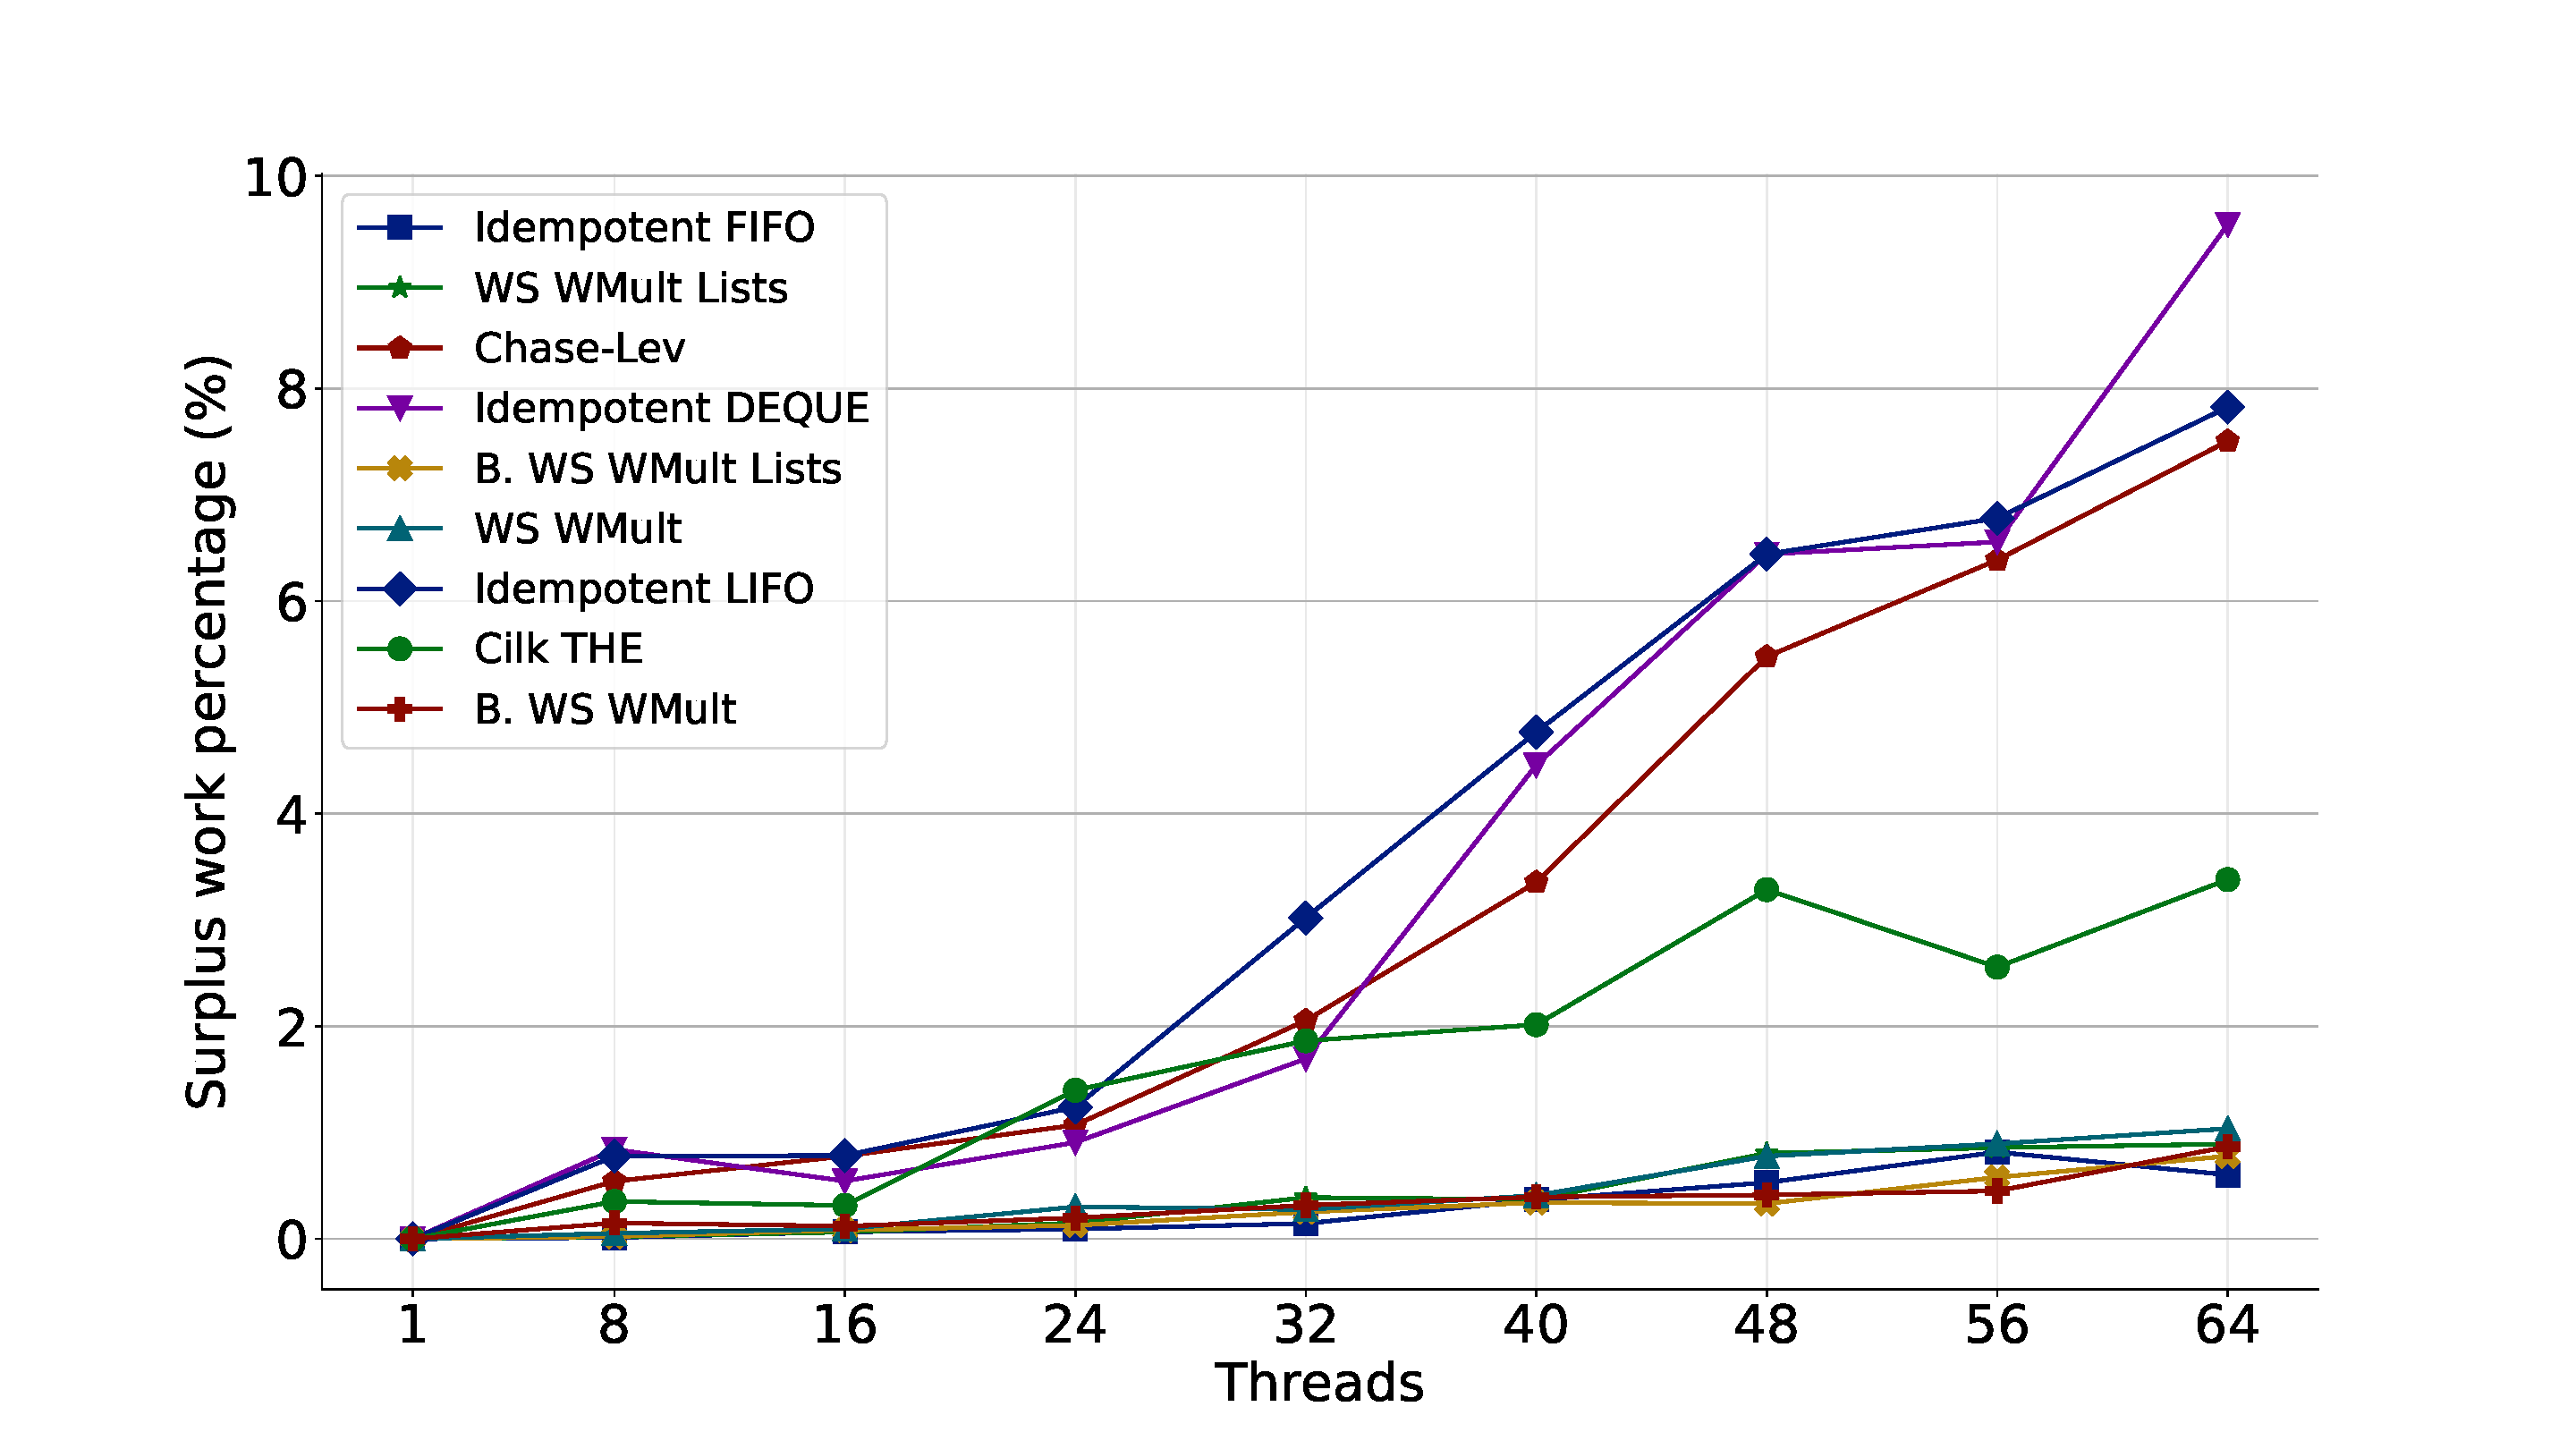
\includegraphics[width=0.48\textwidth]{contents/backmatter/evaluation/mult-torus_3d40_directed_256.pdf}
  }
  \subfloat[\label{fig:surplustorus3d40directed-appx:1000000}Surplus work: Directed Torus 2D 60\%. Initial size of 1,000,000 items]{
    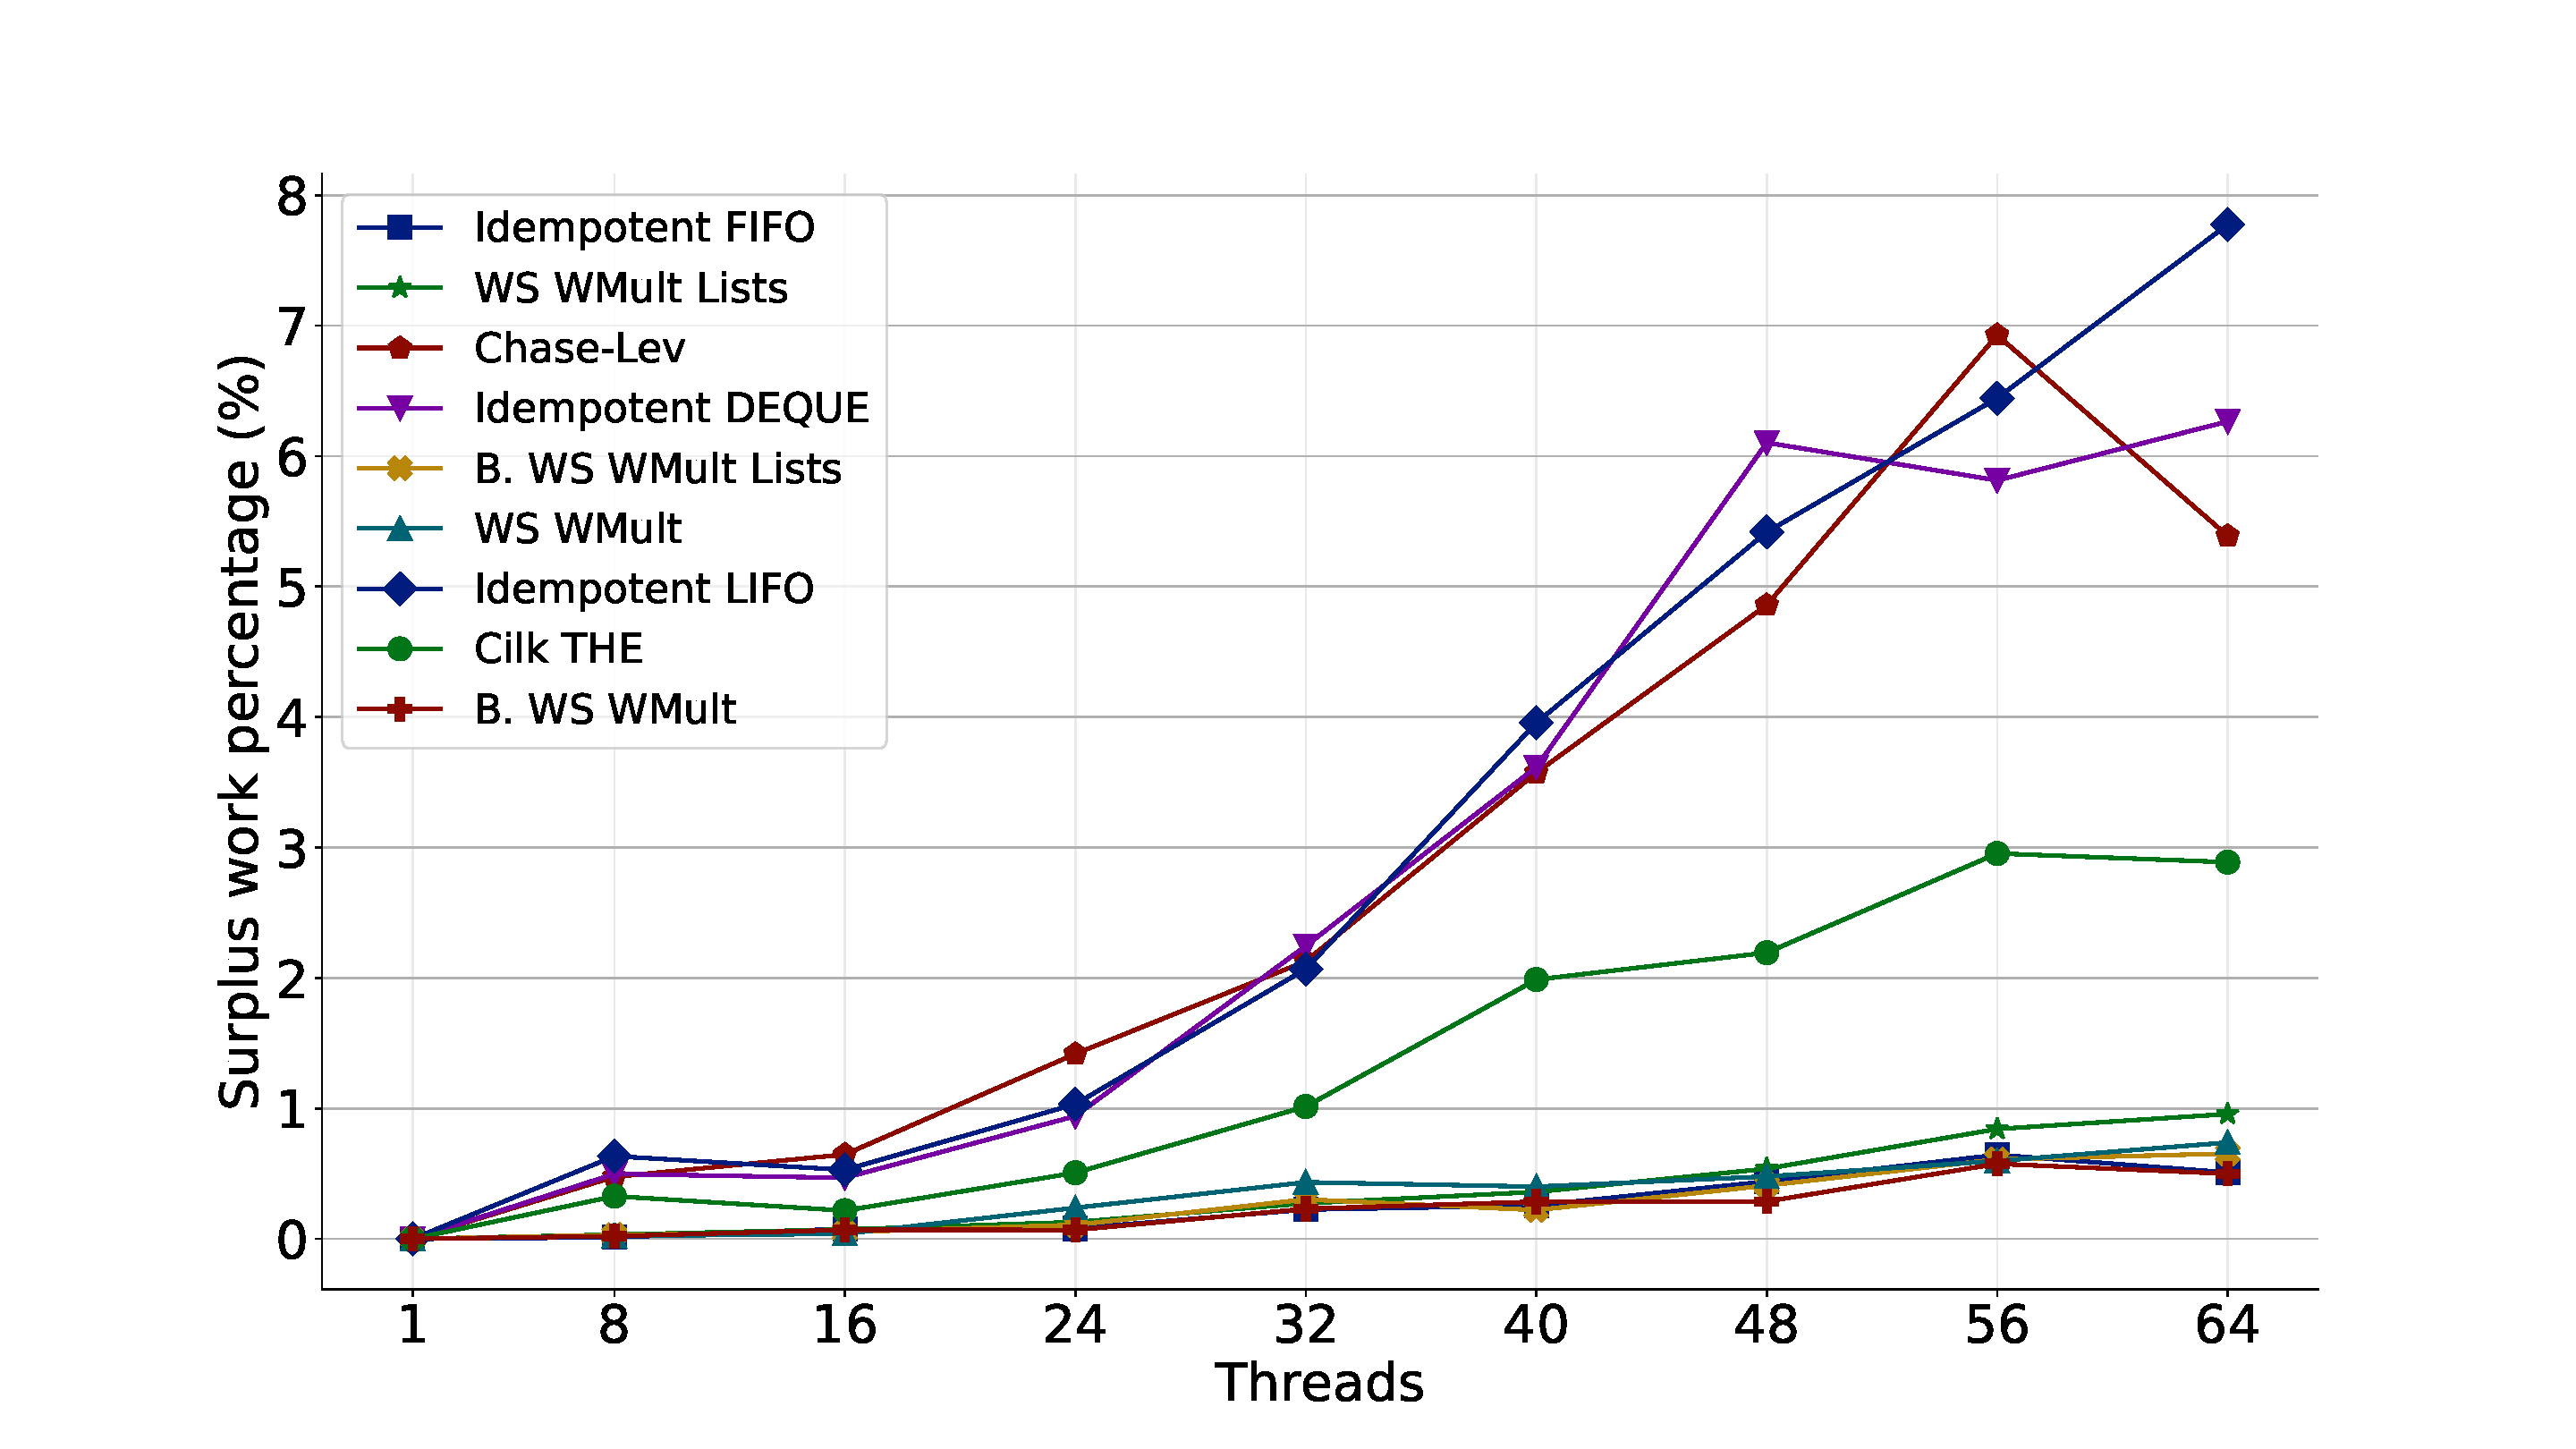
\includegraphics[width=0.48\textwidth]{contents/backmatter/evaluation/mult-torus_3d40_directed_1m.pdf}
  }

  \subfloat[\label{fig:surplustorus3d40undirected-appx:256}Surplus work: Undirected Torus 3D 40\%. Initial size of 256 items]{
    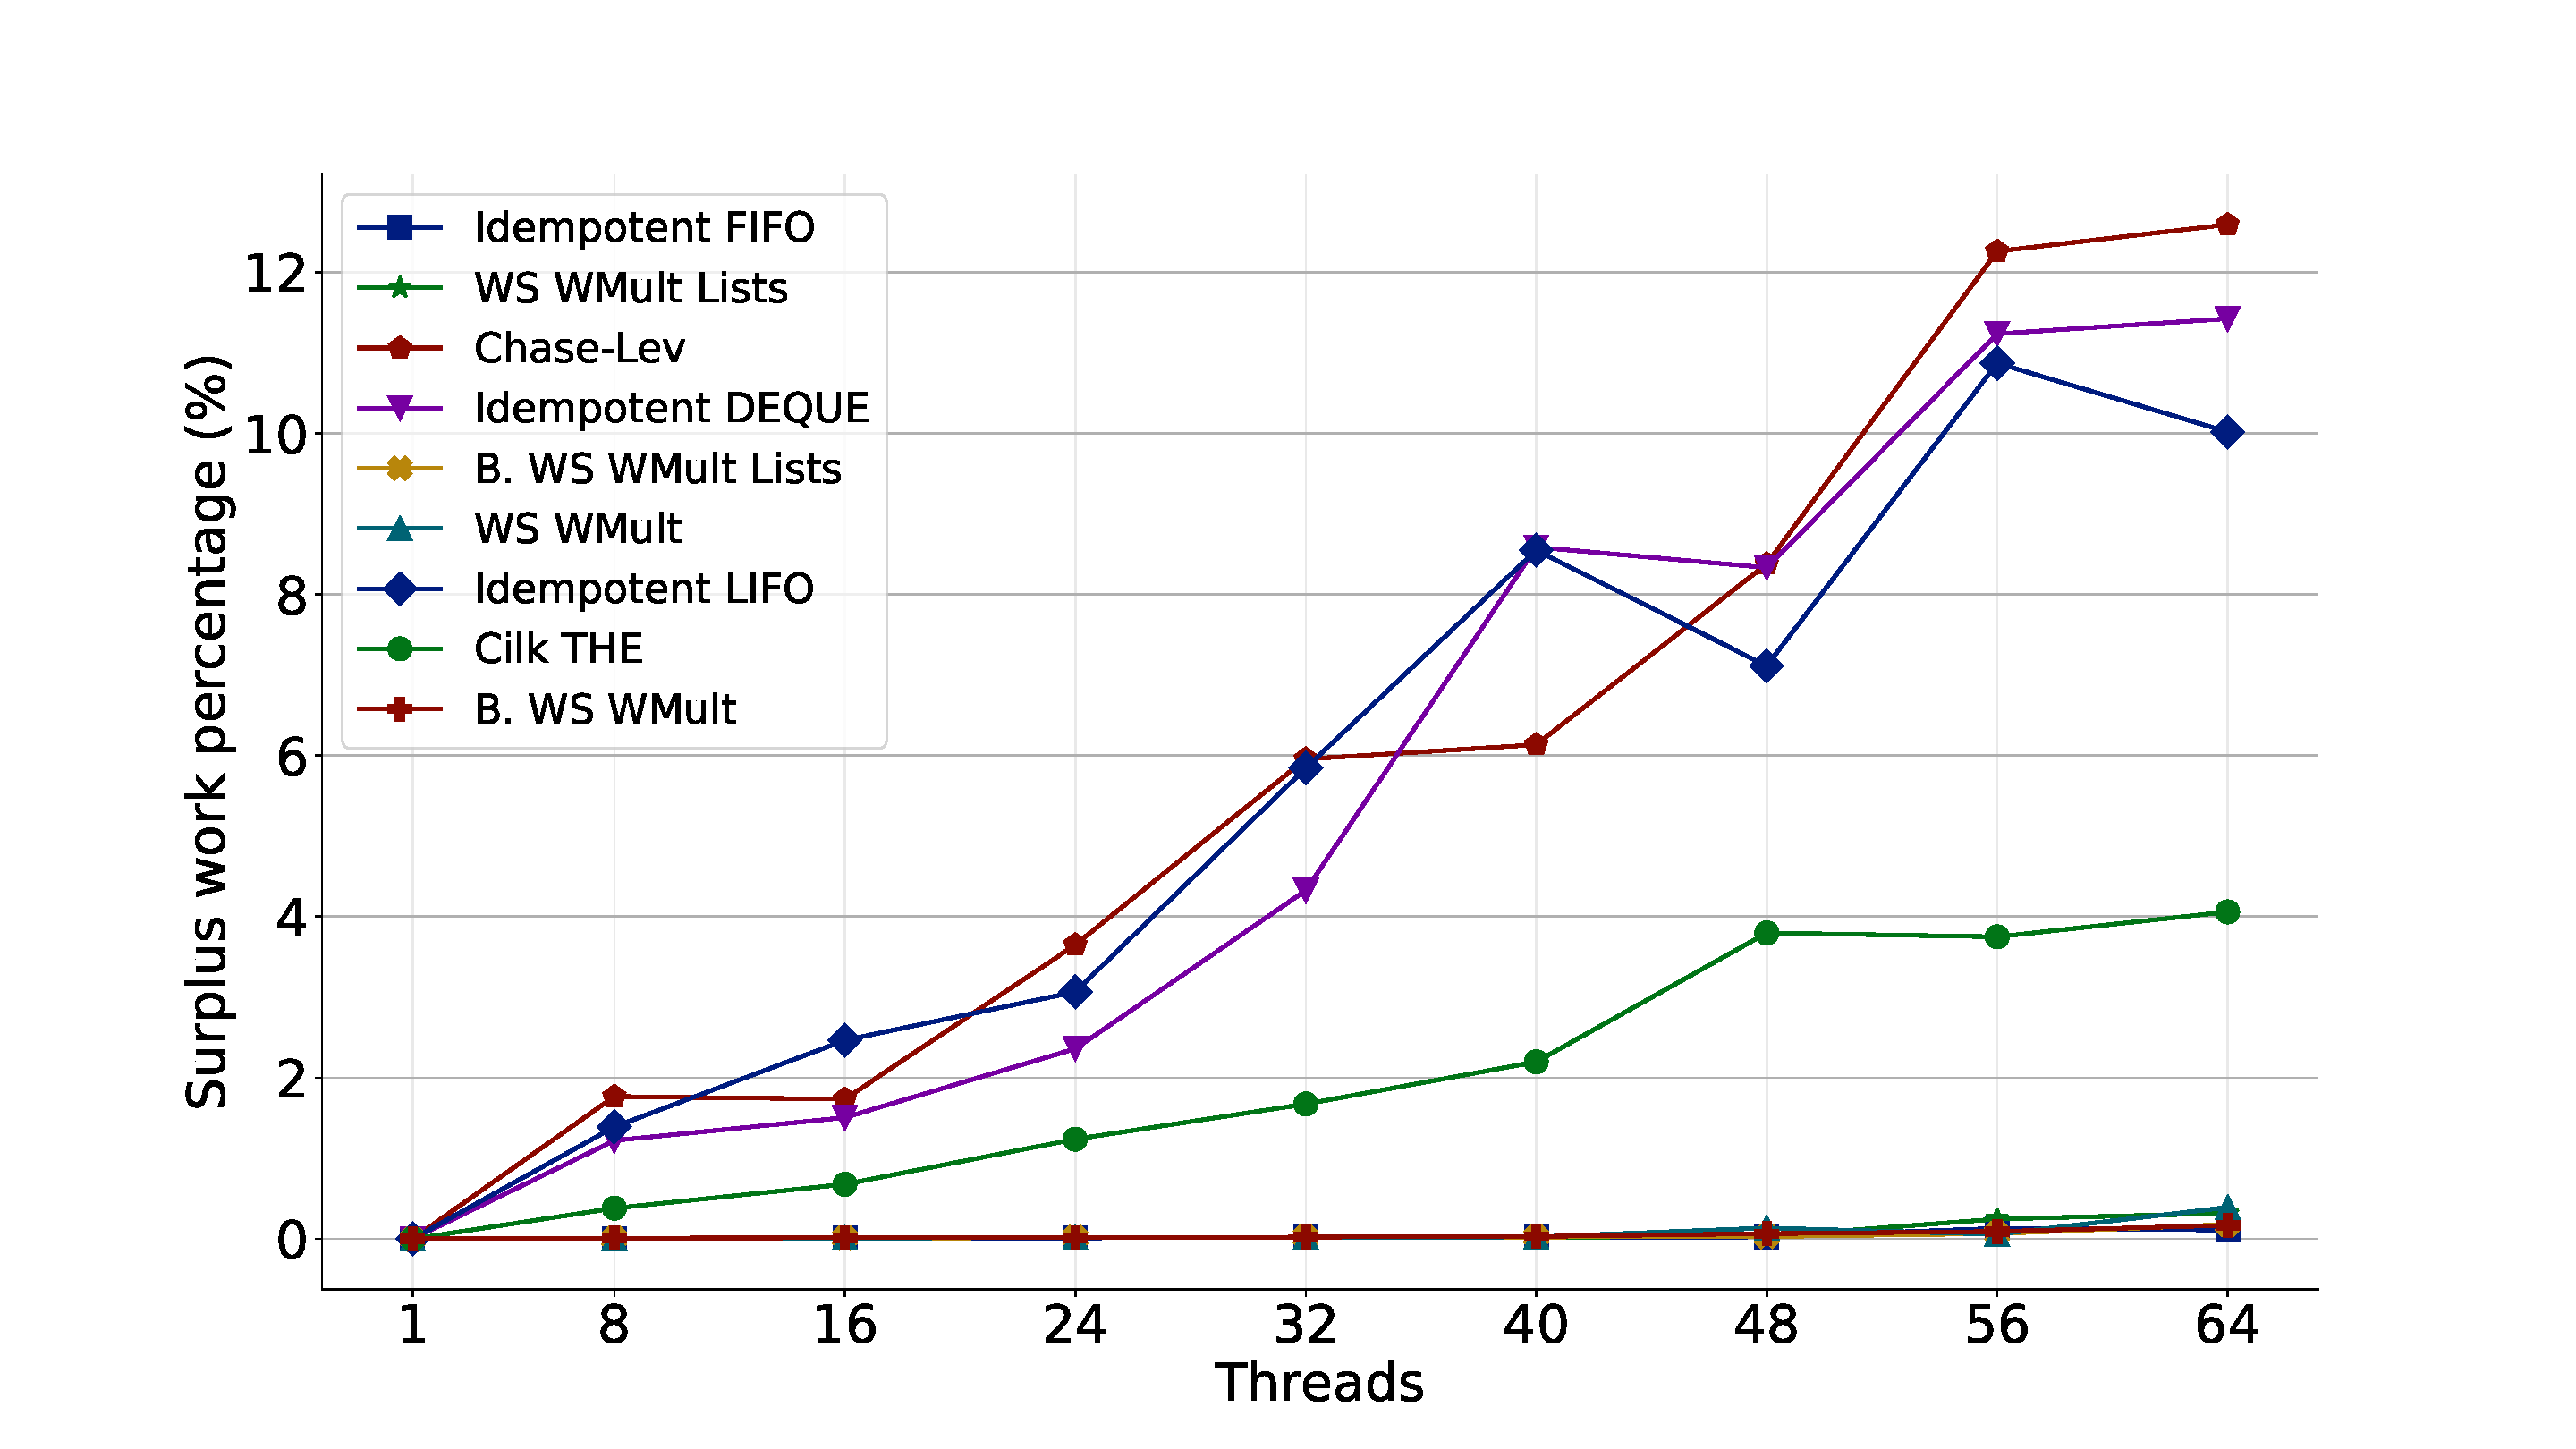
\includegraphics[width=0.48\textwidth]{contents/backmatter/evaluation/mult-torus_3d40_undirected_256.pdf}
  }
  \subfloat[\label{fig:surplustorus3d40undirected:1000000}Surplus work: Undirected Torus 3D 40\%. Initial size of 1,000,000 items]{
    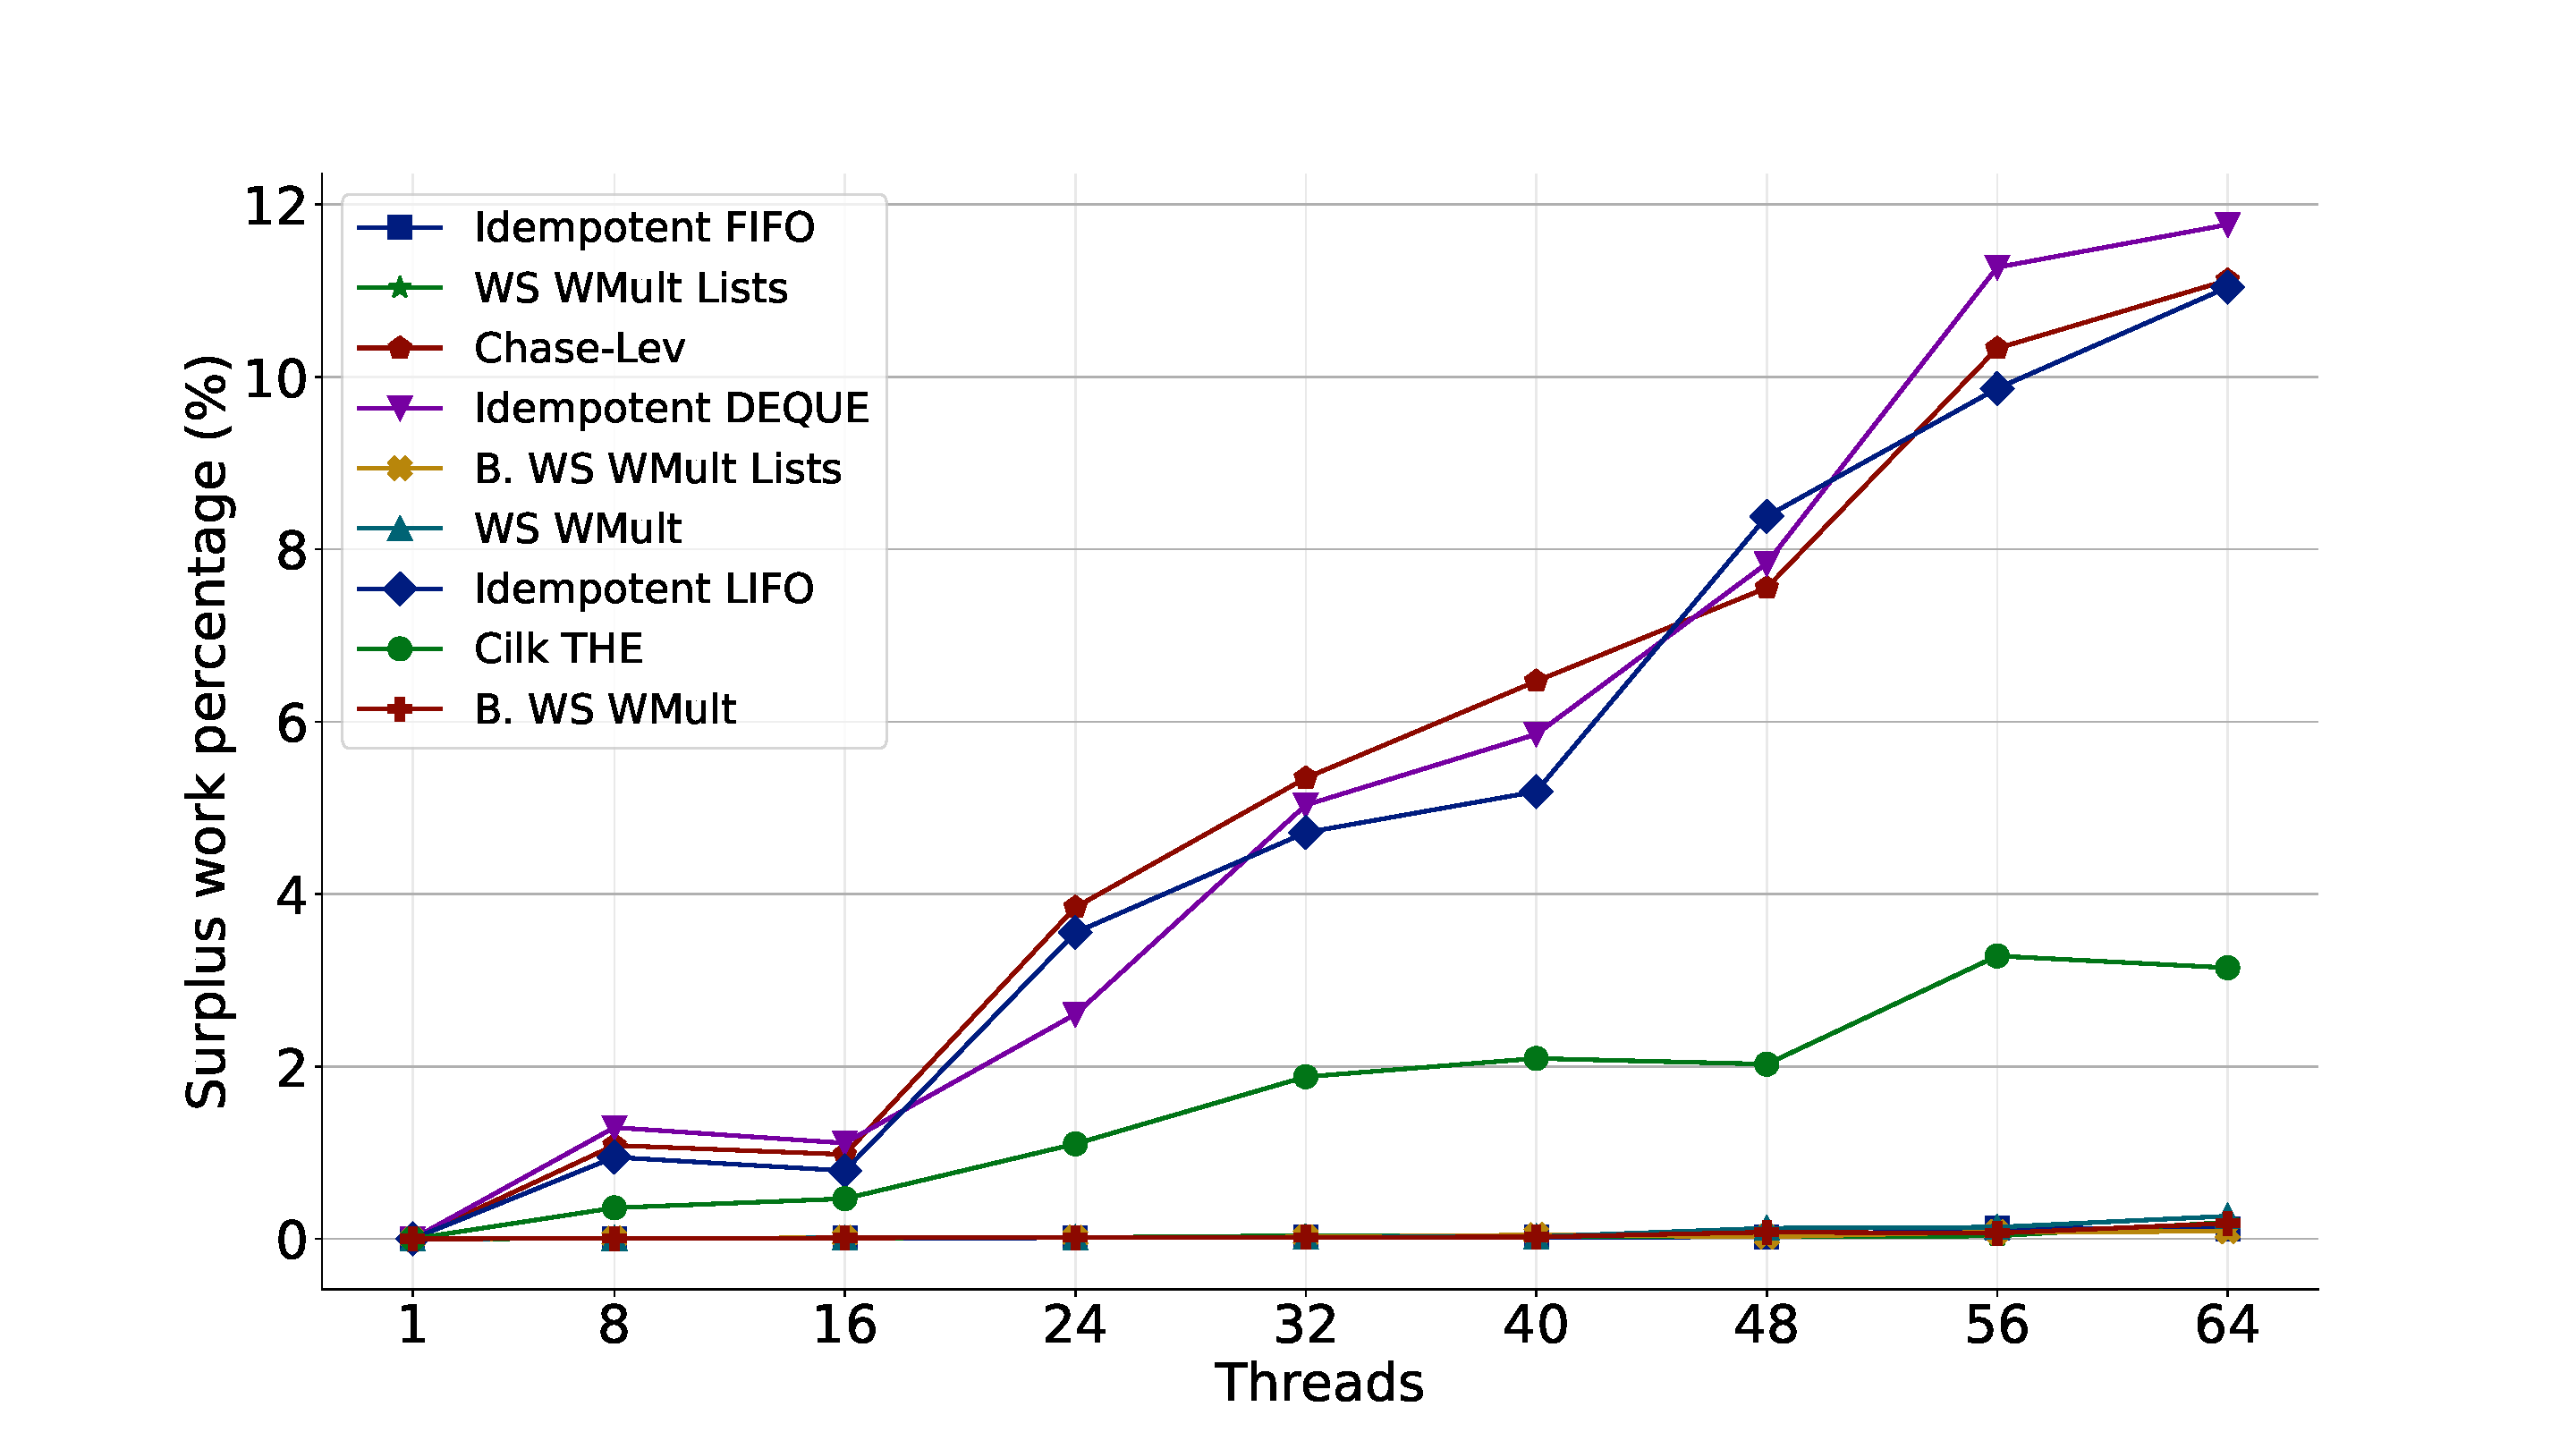
\includegraphics[width=0.48\textwidth]{contents/backmatter/evaluation/mult-torus_3d40_undirected_1m.pdf}
  }

  \caption{\label{fig:surplusgraphapplicationtorus3d40} Surplus work
    (percentage) of the experiments.  Surplus work: the difference
    between the total number of \Puts and the number of puts in
    sequential executions (i.e., $1,000,000$).}
\end{figure}

\begin{figure}[!ht]
  \subfloat[\label{fig:exec-surplustorus3d40directed-appx:256}Executed
  surplus work: Directed Torus 3D 40\%. Initial size of 256 items]{
    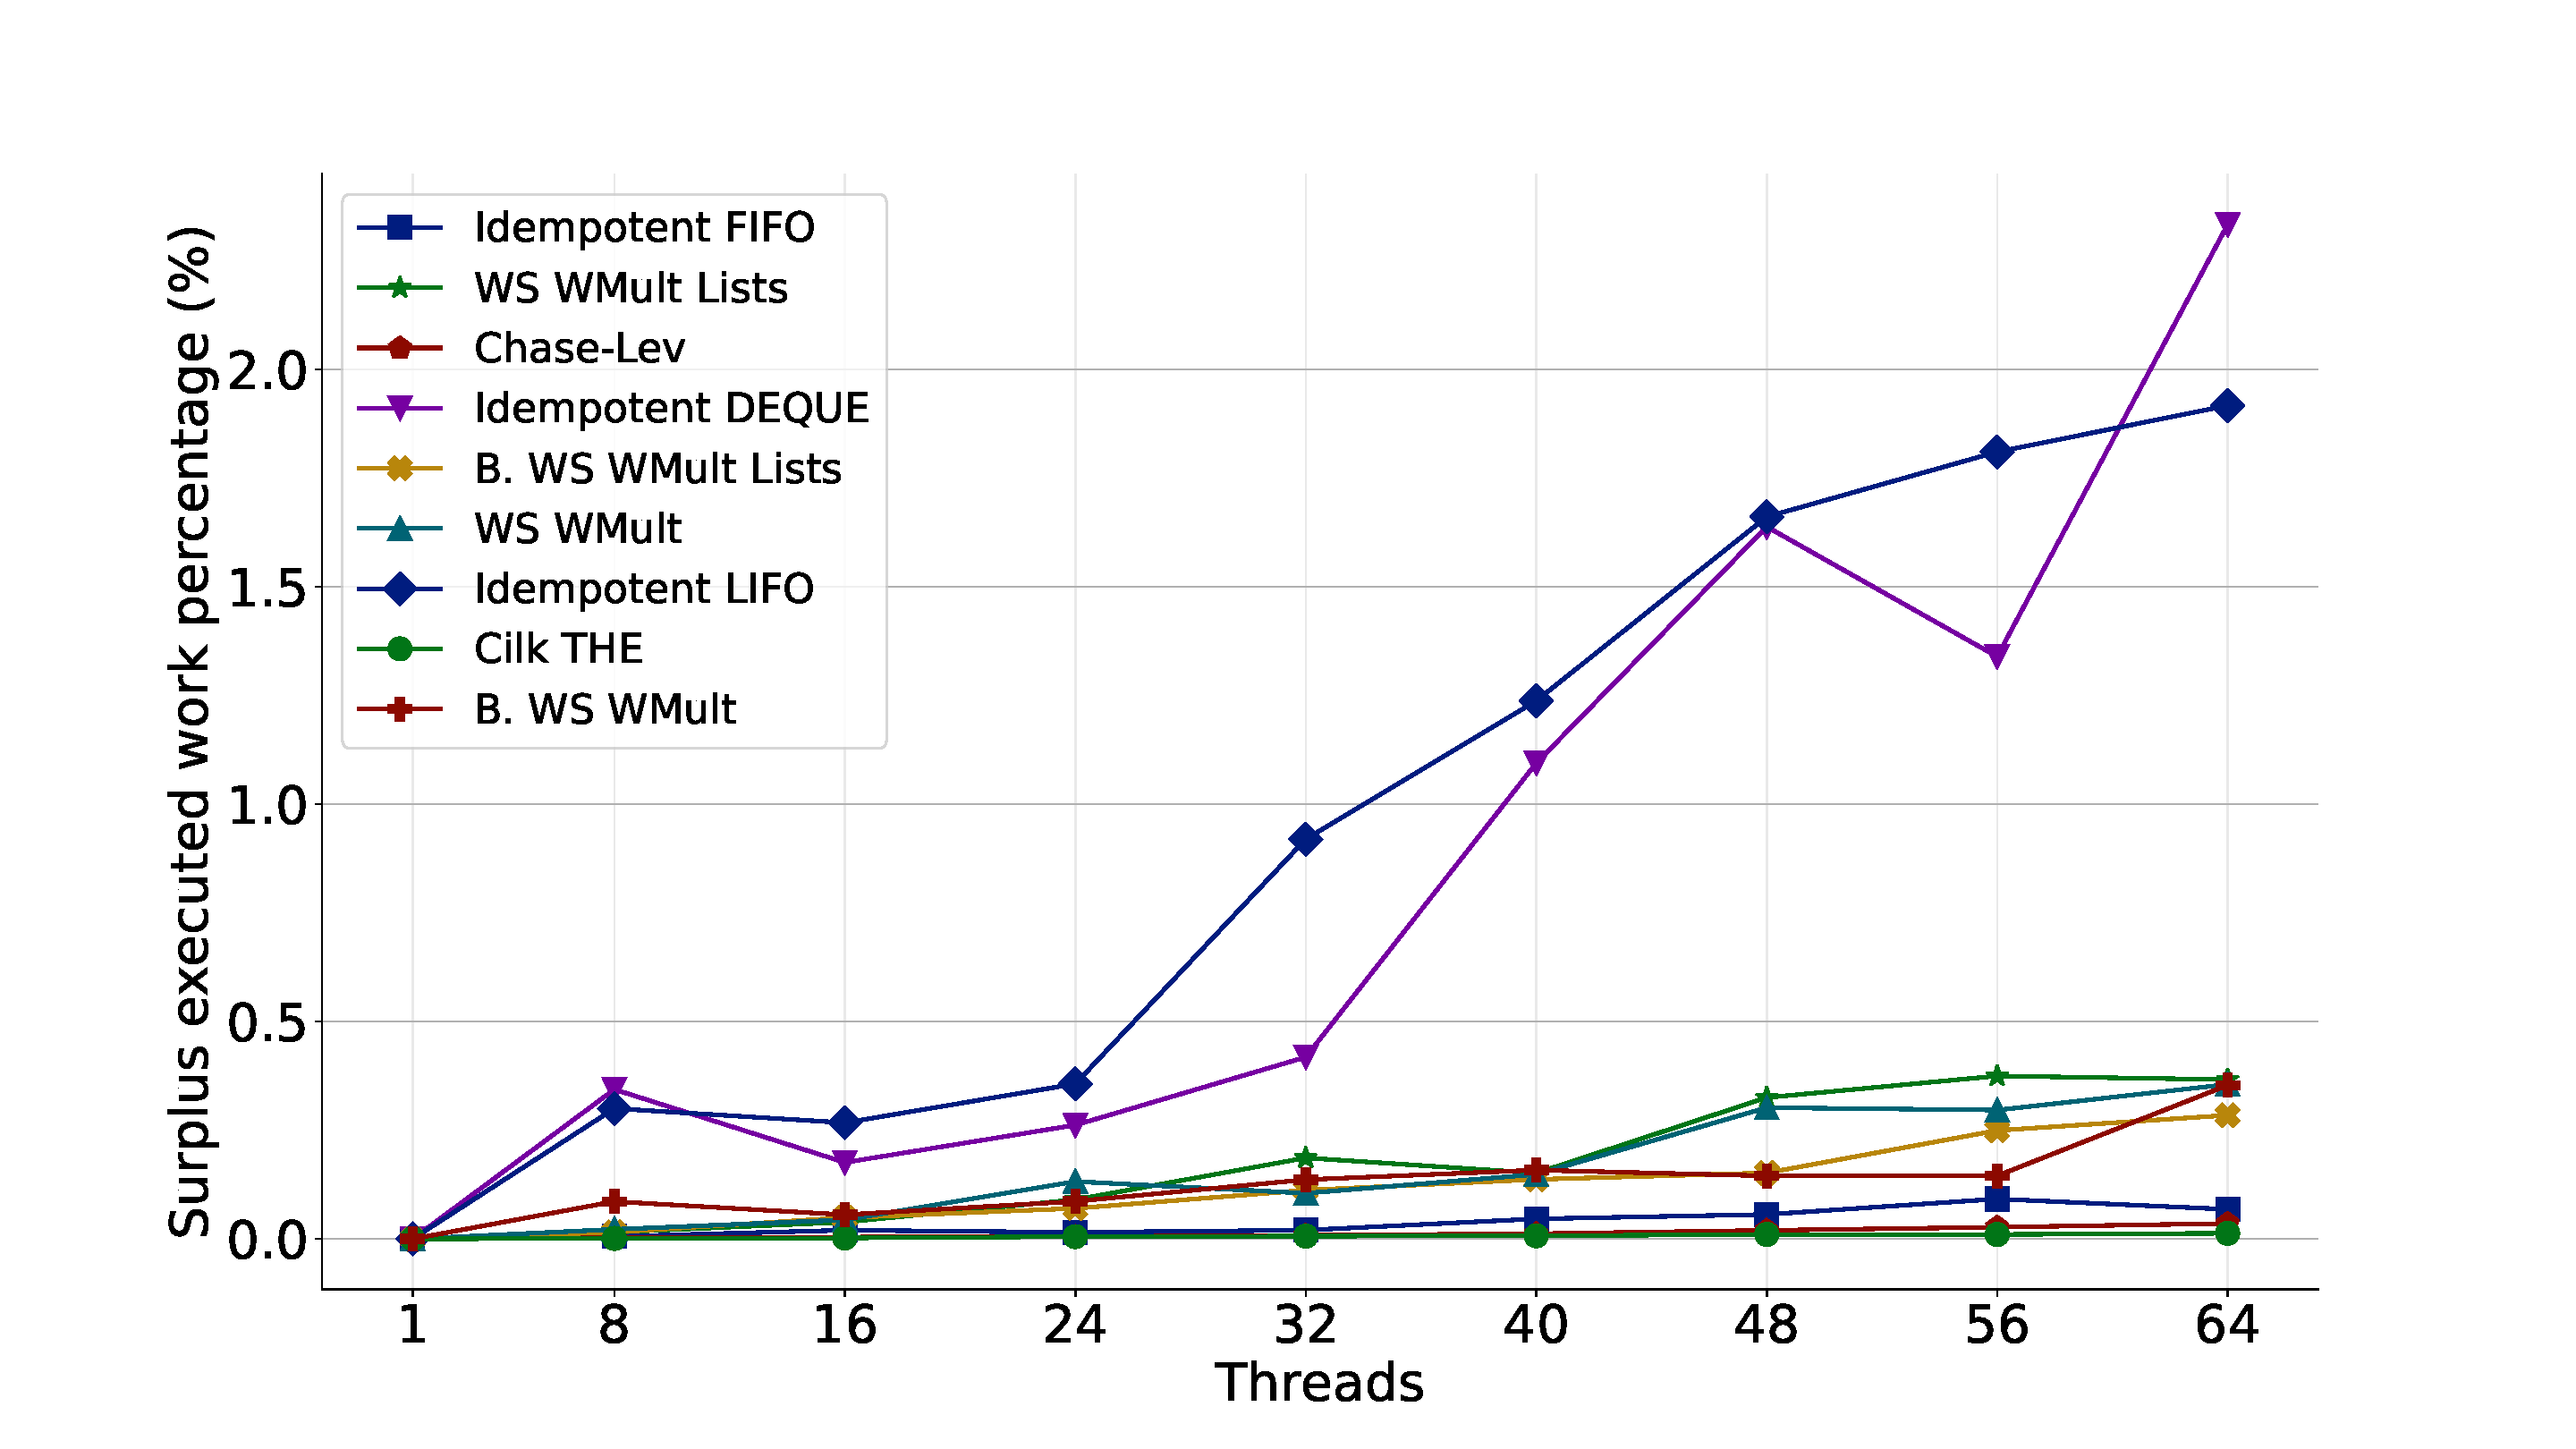
\includegraphics[width=0.48\textwidth]{contents/backmatter/evaluation/mult-exec-torus_3d40_directed_256.pdf}
  }
  \subfloat[\label{fig:exec-surplustorus3d40directed-appx:1000000}Executed
  surplus work: Directed Torus 2D 60\%. Initial size of 1,000,000 items]{
    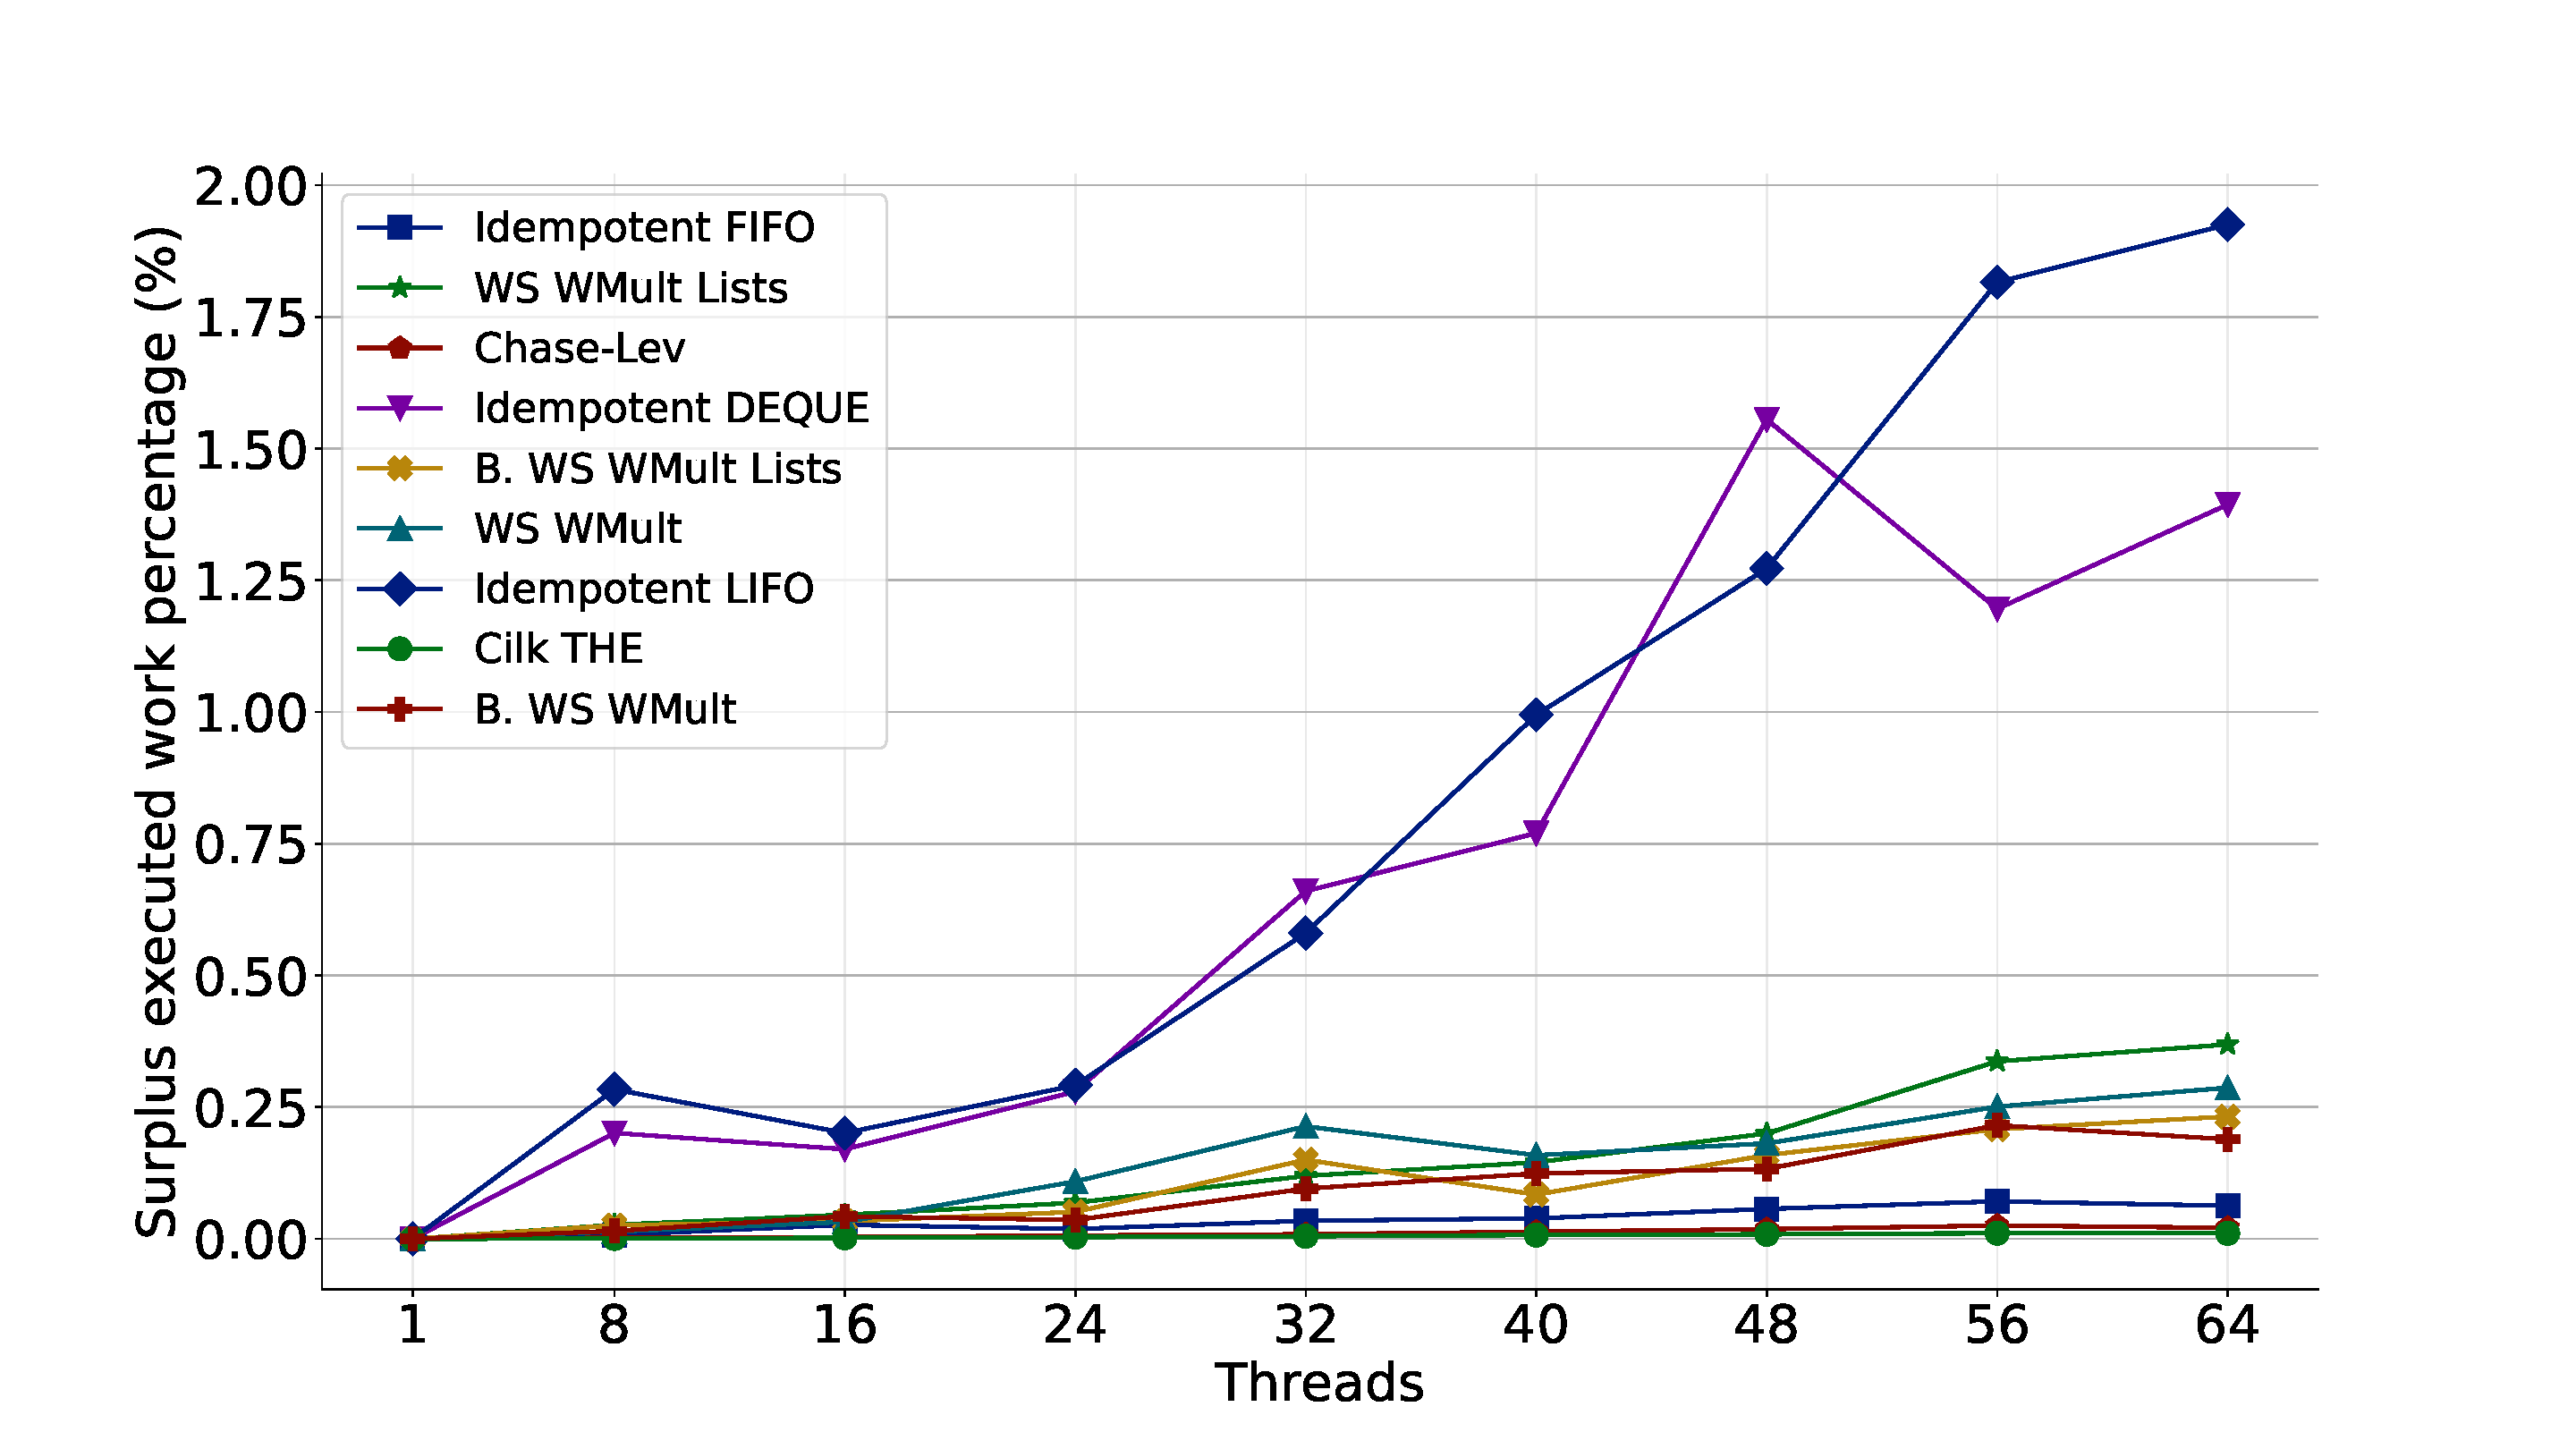
\includegraphics[width=0.48\textwidth]{contents/backmatter/evaluation/mult-exec-torus_3d40_directed_1m.pdf}
  }

  \subfloat[\label{fig:exec-surplustorus3d40undirected-appx:256}Executed
  surplus work: Undirected Torus 3D 40\%. Initial size of 256 items]{
    \includegraphics[width=0.48\textwidth]{contents/backmatter/evaluation/mult-exec-torus_3d40_undirected_256.pdf}
  }
  \subfloat[\label{fig:exec-surplustorus3d40undirected:1000000}Executed
  surplus work: Undirected Torus 3D 40\%. Initial size of 1,000,000 items]{
    \includegraphics[width=0.48\textwidth]{contents/backmatter/evaluation/mult-exec-torus_3d40_undirected_1m.pdf}
  }

  \caption{\label{fig:exec-surplusgraphapplicationtorus3d40} Executed
    surplus work (percentage) of the experiments.  Surplus work: the
    difference between the total number of \Takes and the number of
    takes in sequential executions (i.e., $1,000,000$).}
\end{figure}

\clearpage
\subsubsection{Directed Random. Initial size of 256 items.}
\begin{table}[!ht]
\centering
\resizebox{\textwidth}{!}{\begin{tabular}{lrrrrrrrrrrrrrrr}
\toprule
\textbf{Algorithm} & \multicolumn{5}{l}{Chase-Lev} & \multicolumn{5}{l}{Cilk THE} & \multicolumn{5}{l}{Idempotent LIFO} \\
\textbf{Operation} &       Puts &      Takes & Difference (\%) & Surplus (\%) & Executed Surplus (\%) &       Puts &      Takes & Difference (\%) & Surplus (\%) & Executed Surplus (\%) &            Puts &      Takes & Difference (\%) & Surplus (\%) & Executed Surplus (\%) \\
\textbf{Processes} & \multicolumn{4}{l}{} & \multicolumn{4}{l}{} & \multicolumn{4}{l}{}\\ \midrule
\textbf{1 } & 1000000.00 & 1000000.00 &           0.00 &        0.00 &                 0.00 & 1000000.00 & 1000000.00 &           0.00 &        0.00 &                 0.00 &      1000000.00 & 1000000.00 &           0.00 &        0.00 &                 0.00 \\
\textbf{8 } & 1010376.60 & 1000004.60 &           1.03 &        1.03 &                 0.00 & 1006004.60 & 1000007.00 &           0.60 &        0.60 &                 0.00 &      1009841.20 & 1003227.40 &           0.65 &        0.97 &                 0.32 \\
\textbf{16} & 1013402.20 & 1000012.60 &           1.32 &        1.32 &                 0.00 & 1003361.20 & 1000015.00 &           0.33 &        0.33 &                 0.00 &      1016342.40 & 1004681.00 &           1.15 &        1.61 &                 0.47 \\
\textbf{24} & 1013500.80 & 1000022.60 &           1.33 &        1.33 &                 0.00 & 1009018.20 & 1000024.40 &           0.89 &        0.89 &                 0.00 &      1019164.80 & 1005003.80 &           1.39 &        1.88 &                 0.50 \\
\textbf{28} & 1029575.80 & 1000028.20 &           2.87 &        2.87 &                 0.00 & 1010834.80 & 1000029.60 &           1.07 &        1.07 &                 0.00 &      1043575.20 & 1011793.80 &           3.05 &        4.18 &                 1.17 \\
\textbf{32} & 1030755.60 & 1000028.40 &           2.98 &        2.98 &                 0.00 & 1018235.40 & 1000036.20 &           1.79 &        1.79 &                 0.00 &      1026127.60 & 1006960.80 &           1.87 &        2.55 &                 0.69 \\
\textbf{40} & 1038680.20 & 1000039.40 &           3.72 &        3.72 &                 0.00 & 1020048.60 & 1000042.40 &           1.96 &        1.97 &                 0.00 &      1058921.20 & 1014816.40 &           4.17 &        5.56 &                 1.46 \\
\textbf{48} & 1065990.80 & 1000049.20 &           6.19 &        6.19 &                 0.00 & 1030244.00 & 1000048.80 &           2.93 &        2.94 &                 0.00 &      1089436.60 & 1021604.20 &           6.23 &        8.21 &                 2.11 \\
\textbf{56} & 1093318.80 & 1000055.80 &           8.53 &        8.54 &                 0.01 & 1036149.60 & 1000058.60 &           3.48 &        3.49 &                 0.01 &      1094043.80 & 1022734.20 &           6.52 &        8.60 &                 2.22 \\
\textbf{64} & 1121298.40 & 1000065.20 &          10.81 &       10.82 &                 0.01 & 1037715.40 & 1000064.80 &           3.63 &        3.63 &                 0.01 &      1122813.60 & 1027289.40 &           8.51 &       10.94 &                 2.66 \\
\bottomrule
\end{tabular}}
\label{difference-Random_undirected-256-CHASELEV-CILK-IDEMPOTENT_LIFO}
\caption{The number of puts and takes performed during the
    spanning tree experiment on a Random undirected graph with an initial size
    of 256 items is provided. The table presents data on the
    following algorithms: Chase-Lev, Cilk THE, and
    Idempotent LIFO. Furthermore, we present the percentage difference
    between the number of puts and takes for each available thread,
    relative to the total number of puts. Finally, also we show the
    "surplus" work, which is the difference of the total number of
    \Puts (Work to be scheduled) and the total number of \Puts in
    sequential executions (i.e., 1,000,000), and the "executed surplus
    work", which is the difference between the total number of \Takes
    (actual work executed) and the total of \Takes in sequential
    executions.}
\end{table}

\begin{table}[!ht] \centering
 \resizebox{\textwidth}{!}{\begin{tabular}{lrrrrrrrrrrrrrrr} \toprule
\textbf{Algorithm} & \multicolumn{5}{l}{Idempotent DEQUE} & \multicolumn{5}{l}{Idempotent FIFO} & \multicolumn{5}{l}{WS WMult} \\
\textbf{Operation} &             Puts &      Takes & Difference (\%) & Surplus (\%) & Executed Surplus (\%) &            Puts &      Takes & Difference (\%) & Surplus (\%) & Executed Surplus (\%) &       Puts &      Takes & Difference (\%) & Surplus (\%) & Executed Surplus (\%) \\
\textbf{Processes} & \multicolumn{4}{l}{} & \multicolumn{4}{l}{} & \multicolumn{4}{l}{}\\ \midrule
\textbf{1 } &       1000000.00 & 1000000.00 &           0.00 &        0.00 &                 0.00 &      1000000.00 & 1000000.00 &           0.00 &        0.00 &                 0.00 & 1000000.00 & 1000000.00 &           0.00 &        0.00 &                 0.00 \\
\textbf{8 } &       1007270.40 & 1002469.20 &           0.48 &        0.72 &                 0.25 &      1017301.80 & 1003871.60 &           1.32 &        1.70 &                 0.39 & 1016594.00 & 1007466.80 &           0.90 &        1.63 &                 0.74 \\
\textbf{16} &       1010265.20 & 1003156.80 &           0.70 &        1.02 &                 0.31 &      1020638.60 & 1005089.60 &           1.52 &        2.02 &                 0.51 & 1023145.60 & 1009440.60 &           1.34 &        2.26 &                 0.94 \\
\textbf{24} &       1015514.60 & 1003715.20 &           1.16 &        1.53 &                 0.37 &      1022334.40 & 1004281.20 &           1.77 &        2.18 &                 0.43 & 1031111.00 & 1015066.60 &           1.56 &        3.02 &                 1.48 \\
\textbf{28} &       1016363.20 & 1004100.00 &           1.21 &        1.61 &                 0.41 &      1027849.80 & 1004393.20 &           2.28 &        2.71 &                 0.44 & 1064811.20 & 1026901.40 &           3.56 &        6.09 &                 2.62 \\
\textbf{32} &       1052398.60 & 1013426.00 &           3.70 &        4.98 &                 1.32 &      1049329.80 & 1009179.80 &           3.83 &        4.70 &                 0.91 & 1048733.00 & 1021542.60 &           2.59 &        4.65 &                 2.11 \\
\textbf{40} &       1049780.40 & 1012542.40 &           3.55 &        4.74 &                 1.24 &      1068649.60 & 1009808.20 &           5.51 &        6.42 &                 0.97 & 1087231.20 & 1036120.80 &           4.70 &        8.02 &                 3.49 \\
\textbf{48} &       1086571.00 & 1022005.00 &           5.94 &        7.97 &                 2.15 &      1093902.20 & 1011951.80 &           7.49 &        8.58 &                 1.18 & 1118815.00 & 1051030.60 &           6.06 &       10.62 &                 4.86 \\
\textbf{56} &       1107383.00 & 1027598.00 &           7.20 &        9.70 &                 2.69 &      1099169.80 & 1011793.00 &           7.95 &        9.02 &                 1.17 & 1146516.00 & 1063355.60 &           7.25 &       12.78 &                 5.96 \\
\textbf{64} &       1133525.00 & 1030556.20 &           9.08 &       11.78 &                 2.97 &      1118209.20 & 1015841.20 &           9.15 &       10.57 &                 1.56 & 1170370.40 & 1065732.40 &           8.94 &       14.56 &                 6.17 \\
\bottomrule
\end{tabular}}
\caption{\label{difference-Random_directed-256-IDEMPOTENT_DEQUE-IDEMPOTENT_FIFO-WS_NC_MULT_OPT}The number of puts and takes performed during the
    spanning tree experiment on a Random undirected graph with an initial size
    of 256 items is provided. The table presents data on the
    following algorithms: Idempotent DEQUE, Idempotent FIFO, and
    WS WMult. Furthermore, we present the percentage difference
    between the number of puts and takes for each available thread,
    relative to the total number of puts. Finally, also we show the
    "surplus" work, which is the difference of the total number of
    \Puts (Work to be scheduled) and the total number of \Puts in
    sequential executions (i.e., 1,000,000), and the "executed surplus
    work", which is the difference between the total number of \Takes
    (actual work executed) and the total of \Takes in sequential
    executions.}
\end{table}

\begin{table}[!ht]
\centering
\resizebox{\textwidth}{!}{\begin{tabular}{lrrrrrrrrrrrrrrr}
\toprule
\textbf{Algorithm} & \multicolumn{5}{l}{B. WS WMult} & \multicolumn{5}{l}{WS WMult Lists} & \multicolumn{5}{l}{B. WS WMult Lists} \\
\textbf{Operation} &        Puts &      Takes & Difference (\%) & Surplus (\%) & Executed Surplus (\%) &           Puts &      Takes & Difference (\%) & Surplus (\%) & Executed Surplus (\%) &              Puts &      Takes & Difference (\%) & Surplus (\%) & Executed Surplus (\%) \\
\textbf{Processes} & \multicolumn{4}{l}{} & \multicolumn{4}{l}{} & \multicolumn{4}{l}{}\\ \midrule
\textbf{1 } &  1000000.00 & 1000000.00 &           0.00 &        0.00 &                 0.00 &     1000000.00 & 1000000.00 &           0.00 &        0.00 &                 0.00 &        1000000.00 & 1000000.00 &           0.00 &        0.00 &                 0.00 \\
\textbf{8 } &  1014371.60 & 1008044.20 &           0.62 &        1.42 &                 0.80 &     1014159.80 & 1006525.80 &           0.75 &        1.40 &                 0.65 &        1011005.20 & 1007182.00 &           0.38 &        1.09 &                 0.71 \\
\textbf{16} &  1014463.00 & 1009346.20 &           0.50 &        1.43 &                 0.93 &     1016470.80 & 1008468.60 &           0.79 &        1.62 &                 0.84 &        1014230.00 & 1009122.00 &           0.50 &        1.40 &                 0.90 \\
\textbf{24} &  1024233.20 & 1015111.60 &           0.89 &        2.37 &                 1.49 &     1020183.80 & 1009737.60 &           1.02 &        1.98 &                 0.96 &        1030887.20 & 1020534.80 &           1.00 &        3.00 &                 2.01 \\
\textbf{28} &  1032665.80 & 1019667.00 &           1.26 &        3.16 &                 1.93 &     1027046.00 & 1012317.80 &           1.43 &        2.63 &                 1.22 &        1024738.00 & 1016588.00 &           0.80 &        2.41 &                 1.63 \\
\textbf{32} &  1042648.80 & 1025679.40 &           1.63 &        4.09 &                 2.50 &     1051207.40 & 1021926.80 &           2.79 &        4.87 &                 2.15 &        1031164.60 & 1020148.80 &           1.07 &        3.02 &                 1.98 \\
\textbf{40} &  1054389.60 & 1029050.00 &           2.40 &        5.16 &                 2.82 &     1071398.00 & 1031291.00 &           3.74 &        6.66 &                 3.03 &        1056291.40 & 1032001.60 &           2.30 &        5.33 &                 3.10 \\
\textbf{48} &  1088046.40 & 1040259.40 &           4.39 &        8.09 &                 3.87 &     1108918.40 & 1047254.00 &           5.56 &        9.82 &                 4.51 &        1084315.60 & 1045354.40 &           3.59 &        7.78 &                 4.34 \\
\textbf{56} &  1095902.00 & 1041798.00 &           4.94 &        8.75 &                 4.01 &     1128059.60 & 1055091.80 &           6.47 &       11.35 &                 5.22 &        1091565.20 & 1050216.40 &           3.79 &        8.39 &                 4.78 \\
\textbf{64} &  1180099.80 & 1075089.40 &           8.90 &       15.26 &                 6.98 &     1126343.60 & 1058193.80 &           6.05 &       11.22 &                 5.50 &        1119308.00 & 1058057.60 &           5.47 &       10.66 &                 5.49 \\
\bottomrule
\end{tabular}}
\label{difference-Random_undirected-256-B_WS_NC_MULT_OPT-WS_NC_MULT_LA_OPT-B_WS_NC_MULT_LA_OPT}
\caption{The number of puts and takes performed during the
    spanning tree experiment on a Random undirected graph with an initial size
    of 256 items is provided. The table presents data on the
    following algorithms: B. WS WMult, WS WMult Lists, and
    B. WS WMult Lists. Furthermore, we present the percentage difference
    between the number of puts and takes for each available thread,
    relative to the total number of puts. Finally, also we show the
    "surplus" work, which is the difference of the total number of
    \Puts (Work to be scheduled) and the total number of \Puts in
    sequential executions (i.e., 1,000,000), and the "executed surplus
    work", which is the difference between the total number of \Takes
    (actual work executed) and the total of \Takes in sequential
    executions.}
\end{table}

\clearpage
\subsubsection{Directed Random. Initial size of  1,000,000 items.}
\begin{table}[!ht]
\centering
\resizebox{\textwidth}{!}{\begin{tabular}{lrrrrrrrrrrrrrrr}
\toprule
\textbf{Algorithm} & \multicolumn{5}{l}{Chase-Lev} & \multicolumn{5}{l}{Cilk THE} & \multicolumn{5}{l}{Idempotent LIFO} \\
\textbf{Operation} &       Puts &      Takes & Difference (\%) & Surplus (\%) & Executed Surplus (\%) &       Puts &      Takes & Difference (\%) & Surplus (\%) & Executed Surplus (\%) &            Puts &      Takes & Difference (\%) & Surplus (\%) & Executed Surplus (\%) \\
\textbf{Processes} & \multicolumn{4}{l}{} & \multicolumn{4}{l}{} & \multicolumn{4}{l}{}\\ \midrule
\textbf{1 } & 1000000.00 & 1000000.00 &           0.00 &        0.00 &                 0.00 & 1000000.00 & 1000000.00 &           0.00 &        0.00 &                 0.00 &      1000000.00 & 1000000.00 &           0.00 &        0.00 &                 0.00 \\
\textbf{8 } & 1000018.20 & 1000004.80 &           0.00 &        0.00 &                 0.00 & 1000018.40 & 1000001.80 &           0.00 &        0.00 &                 0.00 &      1000018.80 & 1000006.80 &           0.00 &        0.00 &                 0.00 \\
\textbf{16} & 1000039.40 & 1000009.20 &           0.00 &        0.00 &                 0.00 & 1000041.20 & 1000013.20 &           0.00 &        0.00 &                 0.00 &      1000038.80 & 1000015.60 &           0.00 &        0.00 &                 0.00 \\
\textbf{24} & 1000510.60 & 1000016.40 &           0.05 &        0.05 &                 0.00 & 1000261.60 & 1000013.80 &           0.02 &        0.03 &                 0.00 &      1000133.40 & 1000033.00 &           0.01 &        0.01 &                 0.00 \\
\textbf{28} & 1004930.80 & 1000016.20 &           0.49 &        0.49 &                 0.00 & 1003804.80 & 1000021.60 &           0.38 &        0.38 &                 0.00 &      1004964.60 & 1000489.80 &           0.45 &        0.49 &                 0.05 \\
\textbf{32} & 1005807.00 & 1000016.20 &           0.58 &        0.58 &                 0.00 & 1008753.80 & 1000022.40 &           0.87 &        0.87 &                 0.00 &      1005759.20 & 1000494.80 &           0.52 &        0.57 &                 0.05 \\
\textbf{40} & 1021093.80 & 1000029.80 &           2.06 &        2.07 &                 0.00 & 1018513.20 & 1000031.80 &           1.81 &        1.82 &                 0.00 &      1016913.20 & 1001447.60 &           1.52 &        1.66 &                 0.14 \\
\textbf{48} & 1015945.00 & 1000030.40 &           1.57 &        1.57 &                 0.00 & 1043088.80 & 1000030.00 &           4.13 &        4.13 &                 0.00 &      1025256.60 & 1001997.20 &           2.27 &        2.46 &                 0.20 \\
\textbf{56} & 1060381.80 & 1000043.20 &           5.69 &        5.69 &                 0.00 & 1041672.40 & 1000043.20 &           4.00 &        4.00 &                 0.00 &      1064961.60 & 1005538.20 &           5.58 &        6.10 &                 0.55 \\
\textbf{64} & 1088914.60 & 1000042.40 &           8.16 &        8.17 &                 0.00 & 1049740.00 & 1000050.40 &           4.73 &        4.74 &                 0.01 &      1074591.40 & 1005933.40 &           6.39 &        6.94 &                 0.59 \\
\bottomrule
\end{tabular}}
\label{difference-Random_undirected-1000000-CHASELEV-CILK-IDEMPOTENT_LIFO}
\caption{The number of puts and takes performed during the
    spanning tree experiment on a Random undirected graph with an initial size
    of 1000000 items is provided. The table presents data on the
    following algorithms: Chase-Lev, Cilk THE, and
    Idempotent LIFO. Furthermore, we present the percentage difference
    between the number of puts and takes for each available thread,
    relative to the total number of puts. Finally, also we show the
    "surplus" work, which is the difference of the total number of
    \Puts (Work to be scheduled) and the total number of \Puts in
    sequential executions (i.e., 1,000,000), and the "executed surplus
    work", which is the difference between the total number of \Takes
    (actual work executed) and the total of \Takes in sequential
    executions.}
\end{table}

\begin{table}[!ht]
\centering
\resizebox{\textwidth}{!}{\begin{tabular}{lrrrrrrrrrrrrrrr}
\toprule
\textbf{Algorithm} & \multicolumn{5}{l}{Idempotent DEQUE} & \multicolumn{5}{l}{Idempotent FIFO} & \multicolumn{5}{l}{WS WMult} \\
\textbf{Operation} &             Puts &      Takes & Difference (\%) & Surplus (\%) & Executed Surplus (\%) &            Puts &      Takes & Difference (\%) & Surplus (\%) & Executed Surplus (\%) &       Puts &      Takes & Difference (\%) & Surplus (\%) & Executed Surplus (\%) \\
\textbf{Processes} & \multicolumn{4}{l}{} & \multicolumn{4}{l}{} & \multicolumn{4}{l}{}\\ \midrule
\textbf{1 } &       1000000.00 & 1000000.00 &           0.00 &        0.00 &                 0.00 &      1000000.00 & 1000000.00 &           0.00 &        0.00 &                 0.00 & 1000000.00 & 1000000.00 &           0.00 &        0.00 &                 0.00 \\
\textbf{8 } &       1000020.20 & 1000007.80 &           0.00 &        0.00 &                 0.00 &      1000016.60 & 1000004.00 &           0.00 &        0.00 &                 0.00 & 1000239.60 & 1000098.80 &           0.01 &        0.02 &                 0.01 \\
\textbf{16} &       1000046.60 & 1000019.40 &           0.00 &        0.00 &                 0.00 &      1000027.40 & 1000008.40 &           0.00 &        0.00 &                 0.00 & 1000847.40 & 1000314.20 &           0.05 &        0.08 &                 0.03 \\
\textbf{24} &       1000326.40 & 1000030.80 &           0.03 &        0.03 &                 0.00 &      1001083.00 & 1000074.80 &           0.10 &        0.11 &                 0.01 & 1000951.00 & 1000240.40 &           0.07 &        0.10 &                 0.02 \\
\textbf{28} &       1004643.20 & 1000264.80 &           0.44 &        0.46 &                 0.03 &      1004168.60 & 1000301.00 &           0.39 &        0.42 &                 0.03 & 1005449.60 & 1001284.20 &           0.41 &        0.54 &                 0.13 \\
\textbf{32} &       1006258.40 & 1000273.60 &           0.59 &        0.62 &                 0.03 &      1004946.60 & 1000354.20 &           0.46 &        0.49 &                 0.04 & 1015911.60 & 1003828.00 &           1.19 &        1.57 &                 0.38 \\
\textbf{40} &       1005879.80 & 1000392.60 &           0.55 &        0.58 &                 0.04 &      1012025.00 & 1000774.20 &           1.11 &        1.19 &                 0.08 & 1043118.00 & 1009668.00 &           3.21 &        4.13 &                 0.96 \\
\textbf{48} &       1035772.40 & 1003179.60 &           3.15 &        3.45 &                 0.32 &      1054191.20 & 1004105.20 &           4.75 &        5.14 &                 0.41 & 1022970.40 & 1005817.80 &           1.68 &        2.25 &                 0.58 \\
\textbf{56} &       1072659.20 & 1005832.60 &           6.23 &        6.77 &                 0.58 &      1056553.60 & 1003397.80 &           5.03 &        5.35 &                 0.34 & 1082621.80 & 1019145.80 &           5.86 &        7.63 &                 1.88 \\
\textbf{64} &       1065156.80 & 1004712.00 &           5.67 &        6.12 &                 0.47 &      1119496.00 & 1008768.80 &           9.89 &       10.67 &                 0.87 & 1095691.60 & 1025332.60 &           6.42 &        8.73 &                 2.47 \\
\bottomrule
\end{tabular}}
\label{difference-Random_directed-1000000-IDEMPOTENT_DEQUE-IDEMPOTENT_FIFO-WS_NC_MULT_OPT}
\caption{The number of puts and takes performed during the
    spanning tree experiment on a Random undirected graph with an initial size
    of 1000000 items is provided. The table presents data on the
    following algorithms: Idempotent DEQUE, Idempotent FIFO, and
    WS WMult. Furthermore, we present the percentage difference
    between the number of puts and takes for each available thread,
    relative to the total number of puts. Finally, also we show the
    "surplus" work, which is the difference of the total number of
    \Puts (Work to be scheduled) and the total number of \Puts in
    sequential executions (i.e., 1,000,000), and the "executed surplus
    work", which is the difference between the total number of \Takes
    (actual work executed) and the total of \Takes in sequential
    executions.}
\end{table}

\begin{table}[!ht]
\centering
\resizebox{\textwidth}{!}{\begin{tabular}{lrrrrrrrrrrrrrrr}
\toprule
\textbf{Algorithm} & \multicolumn{5}{l}{B. WS WMult} & \multicolumn{5}{l}{WS WMult Lists} & \multicolumn{5}{l}{B. WS WMult Lists} \\
\textbf{Operation} &        Puts &      Takes & Difference (\%) & Surplus (\%) & Executed Surplus (\%) &           Puts &      Takes & Difference (\%) & Surplus (\%) & Executed Surplus (\%) &              Puts &      Takes & Difference (\%) & Surplus (\%) & Executed Surplus (\%) \\
\textbf{Processes} & \multicolumn{4}{l}{} & \multicolumn{4}{l}{} & \multicolumn{4}{l}{}\\ \midrule
\textbf{1 } &  1000000.00 & 1000000.00 &           0.00 &        0.00 &                 0.00 &     1000000.00 & 1000000.00 &           0.00 &        0.00 &                 0.00 &        1000000.00 & 1000000.00 &           0.00 &        0.00 &                 0.00 \\
\textbf{8 } &  1000013.60 & 1000006.00 &           0.00 &        0.00 &                 0.00 &     1000014.00 & 1000007.20 &           0.00 &        0.00 &                 0.00 &        1000013.40 & 1000006.40 &           0.00 &        0.00 &                 0.00 \\
\textbf{16} &  1000022.60 & 1000015.60 &           0.00 &        0.00 &                 0.00 &     1000026.20 & 1000012.00 &           0.00 &        0.00 &                 0.00 &        1000026.00 & 1000014.80 &           0.00 &        0.00 &                 0.00 \\
\textbf{24} &  1000244.20 & 1000152.20 &           0.01 &        0.02 &                 0.02 &     1000830.40 & 1000105.00 &           0.07 &        0.08 &                 0.01 &        1000042.40 & 1000020.80 &           0.00 &        0.00 &                 0.00 \\
\textbf{28} &  1000964.20 & 1000503.40 &           0.05 &        0.10 &                 0.05 &     1003826.40 & 1000623.40 &           0.32 &        0.38 &                 0.06 &        1003124.00 & 1001179.60 &           0.19 &        0.31 &                 0.12 \\
\textbf{32} &  1005632.20 & 1002692.80 &           0.29 &        0.56 &                 0.27 &     1003712.40 & 1000352.40 &           0.33 &        0.37 &                 0.04 &        1001447.40 & 1000502.40 &           0.09 &        0.14 &                 0.05 \\
\textbf{40} &  1018807.80 & 1007936.60 &           1.07 &        1.85 &                 0.79 &     1017450.80 & 1002580.40 &           1.46 &        1.72 &                 0.26 &        1018311.00 & 1006735.00 &           1.14 &        1.80 &                 0.67 \\
\textbf{48} &  1053572.40 & 1018307.40 &           3.35 &        5.08 &                 1.80 &     1037995.20 & 1006740.60 &           3.01 &        3.66 &                 0.67 &        1033461.40 & 1009894.40 &           2.28 &        3.24 &                 0.98 \\
\textbf{56} &  1035705.00 & 1012473.60 &           2.24 &        3.45 &                 1.23 &     1077590.60 & 1013753.00 &           5.92 &        7.20 &                 1.36 &        1039675.60 & 1011814.60 &           2.68 &        3.82 &                 1.17 \\
\textbf{64} &  1084255.60 & 1027541.80 &           5.23 &        7.77 &                 2.68 &     1076885.20 & 1013112.00 &           5.92 &        7.14 &                 1.29 &        1076659.60 & 1022538.00 &           5.03 &        7.12 &                 2.20 \\
\bottomrule
\end{tabular}}
\label{difference-Random_undirected-1000000-B_WS_NC_MULT_OPT-WS_NC_MULT_LA_OPT-B_WS_NC_MULT_LA_OPT}
\caption{The number of puts and takes performed during the
    spanning tree experiment on a Random undirected graph with an initial size
    of 1000000 items is provided. The table presents data on the
    following algorithms: B. WS WMult, WS WMult Lists, and
    B. WS WMult Lists. Furthermore, we present the percentage difference
    between the number of puts and takes for each available thread,
    relative to the total number of puts. Finally, also we show the
    "surplus" work, which is the difference of the total number of
    \Puts (Work to be scheduled) and the total number of \Puts in
    sequential executions (i.e., 1,000,000), and the "executed surplus
    work", which is the difference between the total number of \Takes
    (actual work executed) and the total of \Takes in sequential
    executions.}
\end{table}

\clearpage
\subsubsection{Undirected Random. Initial size of 256 items.}
\begin{table}[!ht]
\centering
\resizebox{\textwidth}{!}{\begin{tabular}{lrrrrrrrrrrrrrrr}
\toprule
\textbf{Algorithm} & \multicolumn{5}{l}{Chase-Lev} & \multicolumn{5}{l}{Cilk THE} & \multicolumn{5}{l}{Idempotent LIFO} \\
\textbf{Operation} &       Puts &      Takes & Difference (\%) & Surplus (\%) & Executed Surplus (\%) &       Puts &      Takes & Difference (\%) & Surplus (\%) & Executed Surplus (\%) &            Puts &      Takes & Difference (\%) & Surplus (\%) & Executed Surplus (\%) \\
\textbf{Processes} & \multicolumn{4}{l}{} & \multicolumn{4}{l}{} & \multicolumn{4}{l}{}\\ \midrule
\textbf{1 } & 1000000.00 & 1000000.00 &           0.00 &        0.00 &                 0.00 & 1000000.00 & 1000000.00 &           0.00 &        0.00 &                 0.00 &      1000000.00 & 1000000.00 &           0.00 &        0.00 &                 0.00 \\
\textbf{8 } & 1000018.80 & 1000006.00 &           0.00 &        0.00 &                 0.00 & 1000017.40 & 1000004.20 &           0.00 &        0.00 &                 0.00 &      1000020.60 & 1000009.20 &           0.00 &        0.00 &                 0.00 \\
\textbf{16} & 1000476.00 & 1000013.00 &           0.05 &        0.05 &                 0.00 & 1000260.20 & 1000010.20 &           0.02 &        0.03 &                 0.00 &      1000037.20 & 1000017.60 &           0.00 &        0.00 &                 0.00 \\
\textbf{24} & 1000366.20 & 1000013.80 &           0.04 &        0.04 &                 0.00 & 1001121.80 & 1000011.40 &           0.11 &        0.11 &                 0.00 &      1003924.00 & 1000330.40 &           0.36 &        0.39 &                 0.03 \\
\textbf{28} & 1013758.40 & 1000017.00 &           1.36 &        1.36 &                 0.00 & 1001877.80 & 1000011.60 &           0.19 &        0.19 &                 0.00 &      1002989.00 & 1000233.80 &           0.27 &        0.30 &                 0.02 \\
\textbf{32} & 1007197.20 & 1000018.60 &           0.71 &        0.71 &                 0.00 & 1005250.00 & 1000021.40 &           0.52 &        0.52 &                 0.00 &      1002835.00 & 1000186.60 &           0.26 &        0.28 &                 0.02 \\
\textbf{40} & 1020710.20 & 1000030.40 &           2.03 &        2.03 &                 0.00 & 1020256.80 & 1000026.40 &           1.98 &        1.99 &                 0.00 &      1019875.00 & 1001324.00 &           1.82 &        1.95 &                 0.13 \\
\textbf{48} & 1042370.60 & 1000027.40 &           4.06 &        4.06 &                 0.00 & 1046451.00 & 1000038.00 &           4.44 &        4.44 &                 0.00 &      1069346.40 & 1005433.40 &           5.98 &        6.48 &                 0.54 \\
\textbf{56} & 1116503.20 & 1000043.80 &          10.43 &       10.43 &                 0.00 & 1053478.00 & 1000043.80 &           5.07 &        5.08 &                 0.00 &      1080183.40 & 1005619.40 &           6.90 &        7.42 &                 0.56 \\
\textbf{64} & 1113287.80 & 1000048.40 &          10.17 &       10.18 &                 0.00 & 1055949.80 & 1000039.80 &           5.29 &        5.30 &                 0.00 &      1154413.60 & 1012866.80 &          12.26 &       13.38 &                 1.27 \\
\bottomrule
\end{tabular}}
\label{difference-Random_undirected-256-CHASELEV-CILK-IDEMPOTENT_LIFO}
\caption{The number of puts and takes performed during the
    spanning tree experiment on a Random undirected graph with an initial size
    of 256 items is provided. The table presents data on the
    following algorithms: Chase-Lev, Cilk THE, and
    Idempotent LIFO. Furthermore, we present the percentage difference
    between the number of puts and takes for each available thread,
    relative to the total number of puts. Finally, also we show the
    "surplus" work, which is the difference of the total number of
    \Puts (Work to be scheduled) and the total number of \Puts in
    sequential executions (i.e., 1,000,000), and the "executed surplus
    work", which is the difference between the total number of \Takes
    (actual work executed) and the total of \Takes in sequential
    executions.}
\end{table}

\begin{table}[!ht]
\centering
\resizebox{\textwidth}{!}{\begin{tabular}{lrrrrrrrrrrrrrrr}
\toprule
\textbf{Algorithm} & \multicolumn{5}{l}{Idempotent DEQUE} & \multicolumn{5}{l}{Idempotent FIFO} & \multicolumn{5}{l}{WS WMult} \\
\textbf{Operation} &             Puts &      Takes & Difference (\%) & Surplus (\%) & Executed Surplus (\%) &            Puts &      Takes & Difference (\%) & Surplus (\%) & Executed Surplus (\%) &       Puts &      Takes & Difference (\%) & Surplus (\%) & Executed Surplus (\%) \\
\textbf{Processes} & \multicolumn{4}{l}{} & \multicolumn{4}{l}{} & \multicolumn{4}{l}{}\\ \midrule
\textbf{1 } &       1000000.00 & 1000000.00 &           0.00 &        0.00 &                 0.00 &      1000000.00 & 1000000.00 &           0.00 &        0.00 &                 0.00 & 1000000.00 & 1000000.00 &           0.00 &        0.00 &                 0.00 \\
\textbf{8 } &       1000023.00 & 1000010.60 &           0.00 &        0.00 &                 0.00 &      1000015.40 & 1000006.80 &           0.00 &        0.00 &                 0.00 & 1000015.80 & 1000010.00 &           0.00 &        0.00 &                 0.00 \\
\textbf{16} &       1000046.40 & 1000015.80 &           0.00 &        0.00 &                 0.00 &      1000027.00 & 1000011.40 &           0.00 &        0.00 &                 0.00 & 1000027.40 & 1000012.80 &           0.00 &        0.00 &                 0.00 \\
\textbf{24} &       1000339.80 & 1000033.80 &           0.03 &        0.03 &                 0.00 &      1000596.00 & 1000040.20 &           0.06 &        0.06 &                 0.00 & 1002022.60 & 1000278.20 &           0.17 &        0.20 &                 0.03 \\
\textbf{28} &       1000315.00 & 1000030.80 &           0.03 &        0.03 &                 0.00 &      1003849.00 & 1000154.60 &           0.37 &        0.38 &                 0.02 & 1010325.00 & 1001209.60 &           0.90 &        1.02 &                 0.12 \\
\textbf{32} &       1014743.60 & 1001100.40 &           1.34 &        1.45 &                 0.11 &      1015855.80 & 1000799.00 &           1.48 &        1.56 &                 0.08 & 1028760.80 & 1003780.20 &           2.43 &        2.80 &                 0.38 \\
\textbf{40} &       1027781.00 & 1002153.00 &           2.49 &        2.70 &                 0.21 &      1036343.40 & 1001090.60 &           3.40 &        3.51 &                 0.11 & 1029849.60 & 1004925.40 &           2.42 &        2.90 &                 0.49 \\
\textbf{48} &       1052371.40 & 1004724.00 &           4.53 &        4.98 &                 0.47 &      1072843.80 & 1002135.00 &           6.59 &        6.79 &                 0.21 & 1052163.80 & 1007264.60 &           4.27 &        4.96 &                 0.72 \\
\textbf{56} &       1101924.60 & 1009423.20 &           8.39 &        9.25 &                 0.93 &      1089803.00 & 1002223.00 &           8.04 &        8.24 &                 0.22 & 1167712.00 & 1043092.40 &          10.67 &       14.36 &                 4.13 \\
\textbf{64} &       1125583.40 & 1011713.80 &          10.12 &       11.16 &                 1.16 &      1151217.60 & 1004626.40 &          12.73 &       13.14 &                 0.46 & 1161370.00 & 1035727.00 &          10.82 &       13.89 &                 3.45 \\
\bottomrule
\end{tabular}}
\label{difference-Random_undirected-256-IDEMPOTENT_DEQUE-IDEMPOTENT_FIFO-WS_NC_MULT_OPT}
\caption{The number of puts and takes performed during the
    spanning tree experiment on a Random undirected graph with an initial size
    of 256 items is provided. The table presents data on the
    following algorithms: Idempotent DEQUE, Idempotent FIFO, and
    WS WMult. Furthermore, we present the percentage difference
    between the number of puts and takes for each available thread,
    relative to the total number of puts. Finally, also we show the
    "surplus" work, which is the difference of the total number of
    \Puts (Work to be scheduled) and the total number of \Puts in
    sequential executions (i.e., 1,000,000), and the "executed surplus
    work", which is the difference between the total number of \Takes
    (actual work executed) and the total of \Takes in sequential
    executions.}
\end{table}

\begin{table}[!ht]
\centering
\resizebox{\textwidth}{!}{\begin{tabular}{lrrrrrrrrrrrrrrr}
\toprule
\textbf{Algorithm} & \multicolumn{5}{l}{B. WS WMult} & \multicolumn{5}{l}{WS WMult Lists} & \multicolumn{5}{l}{B. WS WMult Lists} \\
\textbf{Operation} &        Puts &      Takes & Difference (\%) & Surplus (\%) & Executed Surplus (\%) &           Puts &      Takes & Difference (\%) & Surplus (\%) & Executed Surplus (\%) &              Puts &      Takes & Difference (\%) & Surplus (\%) & Executed Surplus (\%) \\
\textbf{Processes} & \multicolumn{4}{l}{} & \multicolumn{4}{l}{} & \multicolumn{4}{l}{}\\ \midrule
\textbf{1 } &  1000000.00 & 1000000.00 &           0.00 &        0.00 &                 0.00 &     1000000.00 & 1000000.00 &           0.00 &        0.00 &                 0.00 &        1000000.00 & 1000000.00 &           0.00 &        0.00 &                 0.00 \\
\textbf{8 } &  1000012.00 & 1000006.40 &           0.00 &        0.00 &                 0.00 &     1000013.60 & 1000007.60 &           0.00 &        0.00 &                 0.00 &        1000017.60 & 1000009.80 &           0.00 &        0.00 &                 0.00 \\
\textbf{16} &  1000029.60 & 1000016.20 &           0.00 &        0.00 &                 0.00 &     1000027.00 & 1000015.20 &           0.00 &        0.00 &                 0.00 &        1000028.60 & 1000015.20 &           0.00 &        0.00 &                 0.00 \\
\textbf{24} &  1000135.20 & 1000059.20 &           0.01 &        0.01 &                 0.01 &     1000616.60 & 1000096.80 &           0.05 &        0.06 &                 0.01 &        1000302.20 & 1000142.80 &           0.02 &        0.03 &                 0.01 \\
\textbf{28} &  1003249.60 & 1001104.00 &           0.21 &        0.32 &                 0.11 &     1006872.80 & 1001182.20 &           0.57 &        0.68 &                 0.12 &        1003740.80 & 1001998.80 &           0.17 &        0.37 &                 0.20 \\
\textbf{32} &  1005261.20 & 1001713.20 &           0.35 &        0.52 &                 0.17 &     1011898.00 & 1001469.80 &           1.03 &        1.18 &                 0.15 &        1009561.00 & 1003831.60 &           0.57 &        0.95 &                 0.38 \\
\textbf{40} &  1022896.60 & 1006463.60 &           1.61 &        2.24 &                 0.64 &     1026421.20 & 1004840.00 &           2.10 &        2.57 &                 0.48 &        1024850.20 & 1007092.00 &           1.73 &        2.42 &                 0.70 \\
\textbf{48} &  1049618.40 & 1012988.20 &           3.49 &        4.73 &                 1.28 &     1053696.80 & 1008819.20 &           4.26 &        5.10 &                 0.87 &        1032677.00 & 1009754.60 &           2.22 &        3.16 &                 0.97 \\
\textbf{56} &  1112410.40 & 1027408.40 &           7.64 &       10.11 &                 2.67 &     1130562.40 & 1032846.60 &           8.64 &       11.55 &                 3.18 &        1075503.40 & 1020879.40 &           5.08 &        7.02 &                 2.05 \\
\textbf{64} &  1151473.80 & 1040264.20 &           9.66 &       13.15 &                 3.87 &     1172624.40 & 1048693.60 &          10.57 &       14.72 &                 4.64 &        1109762.60 & 1031496.40 &           7.05 &        9.89 &                 3.05 \\
\bottomrule
\end{tabular}}
\label{difference-Random_undirected-256-B_WS_NC_MULT_OPT-WS_NC_MULT_LA_OPT-B_WS_NC_MULT_LA_OPT}
\caption{The number of puts and takes performed during the
    spanning tree experiment on a Random undirected graph with an initial size
    of 256 items is provided. The table presents data on the
    following algorithms: B. WS WMult, WS WMult Lists, and
    B. WS WMult Lists. Furthermore, we present the percentage difference
    between the number of puts and takes for each available thread,
    relative to the total number of puts. Finally, also we show the
    "surplus" work, which is the difference of the total number of
    \Puts (Work to be scheduled) and the total number of \Puts in
    sequential executions (i.e., 1,000,000), and the "executed surplus
    work", which is the difference between the total number of \Takes
    (actual work executed) and the total of \Takes in sequential
    executions.}
\end{table}

\clearpage
\subsubsection{Undirected Random. Initial size of  1,000,000 items.}
\begin{table}[!ht]
\centering
\resizebox{\textwidth}{!}{\begin{tabular}{lrrrrrrrrrrrrrrrrrrrr}
\toprule
\textbf{Algorithm} & \multicolumn{4}{l}{Chase-Lev} & \multicolumn{4}{l}{Cilk THE} & \multicolumn{4}{l}{Idempotent LIFO} & \multicolumn{4}{l}{Idempotent DEQUE} & \multicolumn{4}{l}{Idempotent FIFO} \\
\textbf{Operation} &       Puts &      Takes & Difference (\%) & Surplus (\%) &       Puts &      Takes & Difference (\%) & Surplus (\%) &            Puts &      Takes & Difference (\%) & Surplus (\%) &             Puts &      Takes & Difference (\%) & Surplus (\%) &            Puts &      Takes & Difference (\%) & Surplus (\%) \\
\textbf{Processes} & \multicolumn{4}{l}{} & \multicolumn{4}{l}{} & \multicolumn{4}{l}{} & \multicolumn{4}{l}{} & \multicolumn{4}{l}{}\\ \midrule
\textbf{1 } & 1000000.00 & 1000000.00 &           0.00 &        0.00 & 1000000.00 & 1000000.00 &           0.00 &        0.00 &      1000000.00 & 1000000.00 &           0.00 &        0.00 &       1000000.00 & 1000000.00 &           0.00 &        0.00 &      1000000.00 & 1000000.00 &           0.00 &        0.00 \\
\textbf{8 } & 1000018.20 & 1000004.80 &           0.00 &        0.00 & 1000018.40 & 1000001.80 &           0.00 &        0.00 &      1000018.80 & 1000006.80 &           0.00 &        0.00 &       1000020.20 & 1000007.80 &           0.00 &        0.00 &      1000016.60 & 1000004.00 &           0.00 &        0.00 \\
\textbf{16} & 1000039.40 & 1000009.20 &           0.00 &        0.00 & 1000041.20 & 1000013.20 &           0.00 &        0.00 &      1000038.80 & 1000015.60 &           0.00 &        0.00 &       1000046.60 & 1000019.40 &           0.00 &        0.00 &      1000027.40 & 1000008.40 &           0.00 &        0.00 \\
\textbf{24} & 1000510.60 & 1000016.40 &           0.05 &        0.05 & 1000261.60 & 1000013.80 &           0.02 &        0.03 &      1000133.40 & 1000033.00 &           0.01 &        0.01 &       1000326.40 & 1000030.80 &           0.03 &        0.03 &      1001083.00 & 1000074.80 &           0.10 &        0.11 \\
\textbf{28} & 1004930.80 & 1000016.20 &           0.49 &        0.49 & 1003804.80 & 1000021.60 &           0.38 &        0.38 &      1004964.60 & 1000489.80 &           0.45 &        0.49 &       1004643.20 & 1000264.80 &           0.44 &        0.46 &      1004168.60 & 1000301.00 &           0.39 &        0.42 \\
\textbf{32} & 1005807.00 & 1000016.20 &           0.58 &        0.58 & 1008753.80 & 1000022.40 &           0.87 &        0.87 &      1005759.20 & 1000494.80 &           0.52 &        0.57 &       1006258.40 & 1000273.60 &           0.59 &        0.62 &      1004946.60 & 1000354.20 &           0.46 &        0.49 \\
\textbf{40} & 1021093.80 & 1000029.80 &           2.06 &        2.07 & 1018513.20 & 1000031.80 &           1.81 &        1.82 &      1016913.20 & 1001447.60 &           1.52 &        1.66 &       1005879.80 & 1000392.60 &           0.55 &        0.58 &      1012025.00 & 1000774.20 &           1.11 &        1.19 \\
\textbf{48} & 1015945.00 & 1000030.40 &           1.57 &        1.57 & 1043088.80 & 1000030.00 &           4.13 &        4.13 &      1025256.60 & 1001997.20 &           2.27 &        2.46 &       1035772.40 & 1003179.60 &           3.15 &        3.45 &      1054191.20 & 1004105.20 &           4.75 &        5.14 \\
\textbf{56} & 1060381.80 & 1000043.20 &           5.69 &        5.69 & 1041672.40 & 1000043.20 &           4.00 &        4.00 &      1064961.60 & 1005538.20 &           5.58 &        6.10 &       1072659.20 & 1005832.60 &           6.23 &        6.77 &      1056553.60 & 1003397.80 &           5.03 &        5.35 \\
\textbf{64} & 1088914.60 & 1000042.40 &           8.16 &        8.17 & 1049740.00 & 1000050.40 &           4.73 &        4.74 &      1074591.40 & 1005933.40 &           6.39 &        6.94 &       1065156.80 & 1004712.00 &           5.67 &        6.12 &      1119496.00 & 1008768.80 &           9.89 &       10.67 \\
\bottomrule
\end{tabular}}
\label{difference-Random_undirected-1000000-CHASELEV-CILK-IDEMPOTENT_LIFO-IDEMPOTENT_DEQUE-IDEMPOTENT_FIFO}
\caption{The number of puts and takes performed during the
    spanning tree experiment on a Random undirected graph with an initial size
    of 1000000 items is provided. The table presents data on the
    following algorithms: Chase-Lev, Cilk THE, Idempotent LIFO, Idempotent DEQUE, and
    Idempotent FIFO. Furthermore, we present the percentage difference
    between the number of puts and takes for each available thread,
    relative to the total number of puts. Finally, also we show the
    "surplus" work, which is the difference of the scheduled tasks and
    the total work avalaible (total of vertices).}
\end{table}

\begin{table}[!ht]
\centering
\resizebox{\textwidth}{!}{\begin{tabular}{lrrrrrrrrrrrrrrr}
\toprule
\textbf{Algorithm} & \multicolumn{5}{l}{Idempotent DEQUE} & \multicolumn{5}{l}{Idempotent FIFO} & \multicolumn{5}{l}{WS WMult} \\
\textbf{Operation} &             Puts &      Takes & Difference (\%) & Surplus (\%) & Executed Surplus (\%) &            Puts &      Takes & Difference (\%) & Surplus (\%) & Executed Surplus (\%) &       Puts &      Takes & Difference (\%) & Surplus (\%) & Executed Surplus (\%) \\
\textbf{Processes} & \multicolumn{4}{l}{} & \multicolumn{4}{l}{} & \multicolumn{4}{l}{}\\ \midrule
\textbf{1 } &       1000000.00 & 1000000.00 &           0.00 &        0.00 &                 0.00 &      1000000.00 & 1000000.00 &           0.00 &        0.00 &                 0.00 & 1000000.00 & 1000000.00 &           0.00 &        0.00 &                 0.00 \\
\textbf{8 } &       1000020.20 & 1000007.80 &           0.00 &        0.00 &                 0.00 &      1000016.60 & 1000004.00 &           0.00 &        0.00 &                 0.00 & 1000239.60 & 1000098.80 &           0.01 &        0.02 &                 0.01 \\
\textbf{16} &       1000046.60 & 1000019.40 &           0.00 &        0.00 &                 0.00 &      1000027.40 & 1000008.40 &           0.00 &        0.00 &                 0.00 & 1000847.40 & 1000314.20 &           0.05 &        0.08 &                 0.03 \\
\textbf{24} &       1000326.40 & 1000030.80 &           0.03 &        0.03 &                 0.00 &      1001083.00 & 1000074.80 &           0.10 &        0.11 &                 0.01 & 1000951.00 & 1000240.40 &           0.07 &        0.10 &                 0.02 \\
\textbf{28} &       1004643.20 & 1000264.80 &           0.44 &        0.46 &                 0.03 &      1004168.60 & 1000301.00 &           0.39 &        0.42 &                 0.03 & 1005449.60 & 1001284.20 &           0.41 &        0.54 &                 0.13 \\
\textbf{32} &       1006258.40 & 1000273.60 &           0.59 &        0.62 &                 0.03 &      1004946.60 & 1000354.20 &           0.46 &        0.49 &                 0.04 & 1015911.60 & 1003828.00 &           1.19 &        1.57 &                 0.38 \\
\textbf{40} &       1005879.80 & 1000392.60 &           0.55 &        0.58 &                 0.04 &      1012025.00 & 1000774.20 &           1.11 &        1.19 &                 0.08 & 1043118.00 & 1009668.00 &           3.21 &        4.13 &                 0.96 \\
\textbf{48} &       1035772.40 & 1003179.60 &           3.15 &        3.45 &                 0.32 &      1054191.20 & 1004105.20 &           4.75 &        5.14 &                 0.41 & 1022970.40 & 1005817.80 &           1.68 &        2.25 &                 0.58 \\
\textbf{56} &       1072659.20 & 1005832.60 &           6.23 &        6.77 &                 0.58 &      1056553.60 & 1003397.80 &           5.03 &        5.35 &                 0.34 & 1082621.80 & 1019145.80 &           5.86 &        7.63 &                 1.88 \\
\textbf{64} &       1065156.80 & 1004712.00 &           5.67 &        6.12 &                 0.47 &      1119496.00 & 1008768.80 &           9.89 &       10.67 &                 0.87 & 1095691.60 & 1025332.60 &           6.42 &        8.73 &                 2.47 \\
\bottomrule
\end{tabular}}
\label{difference-Random_undirected-1000000-IDEMPOTENT_DEQUE-IDEMPOTENT_FIFO-WS_NC_MULT_OPT}
\caption{The number of puts and takes performed during the
    spanning tree experiment on a Random undirected graph with an initial size
    of 1000000 items is provided. The table presents data on the
    following algorithms: Idempotent DEQUE, Idempotent FIFO, and
    WS WMult. Furthermore, we present the percentage difference
    between the number of puts and takes for each available thread,
    relative to the total number of puts. Finally, also we show the
    "surplus" work, which is the difference of the total number of
    \Puts (Work to be scheduled) and the total number of \Puts in
    sequential executions (i.e., 1,000,000), and the "executed surplus
    work", which is the difference between the total number of \Takes
    (actual work executed) and the total of \Takes in sequential
    executions.}
\end{table}

\begin{table}[!ht]
\centering
\resizebox{\textwidth}{!}{\begin{tabular}{lrrrrrrrrrrrrrrr}
\toprule
\textbf{Algorithm} & \multicolumn{5}{l}{B. WS WMult} & \multicolumn{5}{l}{WS WMult Lists} & \multicolumn{5}{l}{B. WS WMult Lists} \\
\textbf{Operation} &        Puts &      Takes & Difference (\%) & Surplus (\%) & Executed Surplus (\%) &           Puts &      Takes & Difference (\%) & Surplus (\%) & Executed Surplus (\%) &              Puts &      Takes & Difference (\%) & Surplus (\%) & Executed Surplus (\%) \\
\textbf{Processes} & \multicolumn{4}{l}{} & \multicolumn{4}{l}{} & \multicolumn{4}{l}{}\\ \midrule
\textbf{1 } &  1000000.00 & 1000000.00 &           0.00 &        0.00 &                 0.00 &     1000000.00 & 1000000.00 &           0.00 &        0.00 &                 0.00 &        1000000.00 & 1000000.00 &           0.00 &        0.00 &                 0.00 \\
\textbf{8 } &  1000013.60 & 1000006.00 &           0.00 &        0.00 &                 0.00 &     1000014.00 & 1000007.20 &           0.00 &        0.00 &                 0.00 &        1000013.40 & 1000006.40 &           0.00 &        0.00 &                 0.00 \\
\textbf{16} &  1000022.60 & 1000015.60 &           0.00 &        0.00 &                 0.00 &     1000026.20 & 1000012.00 &           0.00 &        0.00 &                 0.00 &        1000026.00 & 1000014.80 &           0.00 &        0.00 &                 0.00 \\
\textbf{24} &  1000244.20 & 1000152.20 &           0.01 &        0.02 &                 0.02 &     1000830.40 & 1000105.00 &           0.07 &        0.08 &                 0.01 &        1000042.40 & 1000020.80 &           0.00 &        0.00 &                 0.00 \\
\textbf{28} &  1000964.20 & 1000503.40 &           0.05 &        0.10 &                 0.05 &     1003826.40 & 1000623.40 &           0.32 &        0.38 &                 0.06 &        1003124.00 & 1001179.60 &           0.19 &        0.31 &                 0.12 \\
\textbf{32} &  1005632.20 & 1002692.80 &           0.29 &        0.56 &                 0.27 &     1003712.40 & 1000352.40 &           0.33 &        0.37 &                 0.04 &        1001447.40 & 1000502.40 &           0.09 &        0.14 &                 0.05 \\
\textbf{40} &  1018807.80 & 1007936.60 &           1.07 &        1.85 &                 0.79 &     1017450.80 & 1002580.40 &           1.46 &        1.72 &                 0.26 &        1018311.00 & 1006735.00 &           1.14 &        1.80 &                 0.67 \\
\textbf{48} &  1053572.40 & 1018307.40 &           3.35 &        5.08 &                 1.80 &     1037995.20 & 1006740.60 &           3.01 &        3.66 &                 0.67 &        1033461.40 & 1009894.40 &           2.28 &        3.24 &                 0.98 \\
\textbf{56} &  1035705.00 & 1012473.60 &           2.24 &        3.45 &                 1.23 &     1077590.60 & 1013753.00 &           5.92 &        7.20 &                 1.36 &        1039675.60 & 1011814.60 &           2.68 &        3.82 &                 1.17 \\
\textbf{64} &  1084255.60 & 1027541.80 &           5.23 &        7.77 &                 2.68 &     1076885.20 & 1013112.00 &           5.92 &        7.14 &                 1.29 &        1076659.60 & 1022538.00 &           5.03 &        7.12 &                 2.20 \\
\bottomrule
\end{tabular}}
\label{difference-Random_undirected-1000000-B_WS_NC_MULT_OPT-WS_NC_MULT_LA_OPT-B_WS_NC_MULT_LA_OPT}
\caption{The number of puts and takes performed during the
    spanning tree experiment on a Random undirected graph with an initial size
    of 1000000 items is provided. The table presents data on the
    following algorithms: B. WS WMult, WS WMult Lists, and
    B. WS WMult Lists. Furthermore, we present the percentage difference
    between the number of puts and takes for each available thread,
    relative to the total number of puts. Finally, also we show the
    "surplus" work, which is the difference of the total number of
    \Puts (Work to be scheduled) and the total number of \Puts in
    sequential executions (i.e., 1,000,000), and the "executed surplus
    work", which is the difference between the total number of \Takes
    (actual work executed) and the total of \Takes in sequential
    executions.}
\end{table}


\begin{figure}[!ht]
  \subfloat[\label{fig:surplusrandomdirected-appx:256}Surplus work: Directed Random Graph. Initial size of 256 items]{
    \includegraphics[width=0.48\textwidth]{contents/backmatter/evaluation/mult-random_directed_256.pdf}
  }
  \subfloat[\label{fig:surplusrandomirected-appx:1000000}Surplus work: Directed Random Graph. Initial size of 1,000,000 items]{
    \includegraphics[width=0.48\textwidth]{contents/backmatter/evaluation/mult-random_directed_1m.pdf}
  }

  \subfloat[\label{fig:surplusrandomundirected-appx:256}Surplus work: Undirected Random Graph. Initial size of 256 items]{
    \includegraphics[width=0.48\textwidth]{contents/backmatter/evaluation/mult-random_undirected_256.pdf}
  }
  \subfloat[\label{fig:surplusrandomundirected:1000000}Surplus work: Undirected Random Graph. Initial size of 1,000,000 items]{
    \includegraphics[width=0.48\textwidth]{contents/backmatter/evaluation/mult-random_undirected_1m.pdf}
  }

  \caption{\label{fig:surplusgraphapplicationrandom} Surplus work
    (percentage) of the experiments.  Surplus work: the difference
    between the total number of \Puts and the number of puts in
    sequential executions (i.e., $1,000,000$).}
\end{figure}

\begin{figure}[!ht]
  \subfloat[\label{fig:exec-surplusrandomdirected-appx:256}Executed surplus work: Directed Random Graph. Initial size of 256 items]{
    \includegraphics[width=0.48\textwidth]{contents/backmatter/evaluation/mult-exec-random_directed_256.pdf}
  }
  \subfloat[\label{fig:exec-surplusrandomirected-appx:1000000}Executed
  surplus work: Directed Random Graph. Initial size of 1,000,000 items]{
    \includegraphics[width=0.48\textwidth]{contents/backmatter/evaluation/mult-exec-random_directed_1m.pdf}
  }

  \subfloat[\label{fig:exec-surplusrandomundirected-appx:256}Executed surplus work: Undirected Random Graph. Initial size of 256 items]{
    \includegraphics[width=0.48\textwidth]{contents/backmatter/evaluation/mult-exec-random_undirected_256.pdf}
  }
  \subfloat[\label{fig:exec-surplusrandomundirected:1000000}Executed surplus work: Undirected Random Graph. Initial size of 1,000,000 items]{
    \includegraphics[width=0.48\textwidth]{contents/backmatter/evaluation/mult-exec-random_undirected_1m.pdf}
  }

  \caption{\label{fig:exec-surplusgraphapplicationrandom} Executed surplus
    work (percentage) of the experiments.  Surplus work: the
    difference between the total number of \Takes and the number of
    takes in sequential executions (i.e., $1,000,000$).  }
\end{figure}

\clearpage{}

\section{\label{sec:sat-appendix}Results of SAT experiment}

This section presents the measurements from the parallel SAT experiment. Shows the results for the different ranges with which the parallel job was tested. Measurements were made using rigorous statistical methodology. This evaluation was performed for all work-stealing algorithms. Additionally, the percentage of repeated work is shown as the number of takes plus steals made. This is easily measurable because there is only one work-stealing structure with a single producer and multiple consumers. The owner of the structure calls the take method every time it is going to process a task, and the other workers call the steal method. Therefore, the number of puts is always fixed, while the sum of takes and puts is at least the total amount of work that was inserted via the put method.

\begin{figure}[!ht]

  \subfloat[\label{fig:sat:50:1:appendix}Range assigment size 50.]{
    \includegraphics[width=0.48\textwidth]{contents/backmatter/evaluation/sat-50-1.pdf}
  }
  \subfloat[\label{fig:sat:50:2:appendix}Ranges assignment size
  50. Zoom into the number of processes 32 to 64.]{
    \includegraphics[width=0.48\textwidth]{contents/backmatter/evaluation/sat-50-2.pdf}
  }

  \caption{\label{fig:satapplication:50} Mean times of the Parallel
    SAT benchmark for range assignment 50.}
\end{figure}

\begin{table}[!ht]
\centering
\resizebox{\textwidth}{!}{\begin{tabular}{lrrrrrrrrrrrrrrrrr}
\toprule{} &            1  &            4  &            8  &            12 &            16 &            20 &            24 &            28 &            32 &            36 &            40 &            44 &            48 &            52 &            56 &            60 &            64 \\
\midrule
\textbf{Chase-Lev       } & 6771106493.51 & 1889235456.63 & 1604639874.37 & 1619823677.67 & 1646573644.81 & 1673070572.69 & 1687294862.61 & 1696749620.63 & 1703680039.41 & 1710985761.03 & 1715687626.59 & 1720808375.81 & 1725459846.29 & 1729465873.47 & 1733202358.64 & 1736669234.59 & 1739748595.84 \\
\textbf{Cilk THE        } & 6802197168.26 & 1933130275.93 & 1610054131.24 & 1625700961.91 & 1652168564.44 & 1678643423.36 & 1693219776.67 & 1700315677.49 & 1704476100.71 & 1710217427.63 & 1715966400.77 & 1721428221.41 & 1726061148.66 & 1729668882.90 & 1733466762.36 & 1730280495.31 & 1722706049.09 \\
\textbf{Idempotent LIFO } & 6765613525.70 & 1889322149.43 & 1604852066.19 & 1620383537.76 & 1646698759.04 & 1672839289.99 & 1687124110.16 & 1696275853.74 & 1704046387.47 & 1709655019.76 & 1716006135.71 & 1721069733.01 & 1725560718.04 & 1729361763.40 & 1733293132.63 & 1736993631.74 & 1739532414.24 \\
\textbf{Idempotent FIFO } & 6777176155.51 & 1889535666.67 & 1606530877.24 & 1619900006.93 & 1646961802.84 & 1672795260.39 & 1686690773.01 & 1696541623.33 & 1703370023.54 & 1709696507.80 & 1714958659.79 & 1720376563.60 & 1724996570.13 & 1729562393.91 & 1734432732.00 & 1736538220.60 & 1740059007.49 \\
\textbf{Idempotent DEQUE} & 6754222054.47 & 1887515675.74 & 1607441806.56 & 1620652684.31 & 1646659093.64 & 1672990966.89 & 1687002947.97 & 1696362167.43 & 1703012345.57 & 1709754367.74 & 1715467579.27 & 1720232884.76 & 1724737751.76 & 1728808479.63 & 1732979869.21 & 1736495267.69 & 1739516302.51 \\
\textbf{WS Mult.        } & 6759188962.90 & 1895287204.46 & 1608931490.97 & 1626576516.29 & 1653947113.14 & 1681567490.83 & 1697659943.97 & 1710112808.26 & 1722093689.80 & 1731664198.24 & 1742294997.76 & 1751311084.83 & 1759492255.69 & 1768839583.80 & 1776646590.17 & 1784288295.49 & 1790959219.97 \\
\textbf{B. WS Mult.     } & 6749674804.90 & 1891140517.30 & 1606570003.57 & 1621611512.86 & 1648643759.01 & 1674782575.49 & 1688764361.97 & 1697863713.51 & 1704635152.71 & 1710999825.43 & 1717298452.77 & 1722122072.69 & 1726707115.19 & 1731157469.19 & 1734667658.91 & 1737970629.40 & 1740941783.40 \\
\bottomrule
\end{tabular}}
\label{sat-50-stats}
\caption{Resulting mean times for the SAT benchmark. These are the results for tasks with 50 assignments.}
\end{table}


\clearpage

\begin{figure}[!ht]
  \subfloat[\label{fig:sat:100:1}Range assignment size 100.]{
    \includegraphics[width=0.48\textwidth]{contents/backmatter/evaluation/sat-100-1.pdf}
  }
  \subfloat[\label{fig:sat:100:2}Ranges assignment size 100. Zoom into
  the number of processes 32 to 64.]{
    \includegraphics[width=0.48\textwidth]{contents/backmatter/evaluation/sat-100-2.pdf}
  }

  \caption{\label{fig:satapplication:100} Mean times of the Parallel
    SAT benchmark for range assignment 100.}
\end{figure}

\begin{table}[!ht]
\centering
\resizebox{\textwidth}{!}{\begin{tabular}{lrrrrrrrrrrrrrrrrr}
\toprule{} &            1  &            4  &            8  &            12 &            16 &            20 &            24 &            28 &            32 &            36 &            40 &            44 &            48 &            52 &            56 &            60 &            64 \\
\midrule
\textbf{Chase-Lev       } & 6681894196.79 & 1878532981.09 & 1607198238.76 & 1619373794.26 & 1646161727.76 & 1672418279.90 & 1686050945.86 & 1695660527.96 & 1702542263.80 & 1709612160.87 & 1715821031.64 & 1720880142.11 & 1725753779.47 & 1729752224.94 & 1733896976.53 & 1736565443.89 & 1739731314.63 \\
\textbf{Cilk THE        } & 6713144570.01 & 1907821954.13 & 1608959290.14 & 1625924986.24 & 1650636064.94 & 1677254077.36 & 1691318036.30 & 1700170199.61 & 1703303768.40 & 1710257851.40 & 1716483961.57 & 1721373546.30 & 1726313143.23 & 1730158320.93 & 1733852571.80 & 1737180435.81 & 1740086113.23 \\
\textbf{Idempotent LIFO } & 6683734211.79 & 1879640341.39 & 1605755065.69 & 1619557166.63 & 1646749050.20 & 1672605855.71 & 1686356001.69 & 1695418620.26 & 1702768108.47 & 1709845572.26 & 1715641938.47 & 1720572054.74 & 1725680760.97 & 1729833982.57 & 1733560046.70 & 1736864400.26 & 1739675502.83 \\
\textbf{Idempotent FIFO } & 6663575563.97 & 1874581080.89 & 1605273186.81 & 1619821900.27 & 1646469758.39 & 1672356605.59 & 1686321505.14 & 1696049308.93 & 1702713437.63 & 1709494167.00 & 1715453752.30 & 1720722648.44 & 1725673225.36 & 1729568516.90 & 1733430752.01 & 1736873945.57 & 1739588215.41 \\
\textbf{Idempotent DEQUE} & 6677808307.77 & 1878565281.23 & 1605869783.66 & 1619938274.40 & 1646046886.26 & 1672922371.53 & 1686246470.23 & 1696015949.89 & 1702965954.56 & 1708681178.37 & 1715512242.60 & 1720354719.36 & 1725544754.73 & 1729265270.43 & 1733664563.41 & 1736726526.67 & 1739877762.29 \\
\textbf{WS Mult.        } & 6655863065.41 & 1881147196.97 & 1607518117.34 & 1623255189.83 & 1650666167.06 & 1677309219.59 & 1692459616.23 & 1703860952.49 & 1713270314.14 & 1721989747.53 & 1730125346.56 & 1737926826.01 & 1744710003.79 & 1751353566.93 & 1758374969.06 & 1763599554.51 & 1768917861.41 \\
\textbf{B. WS Mult.     } & 6681927524.90 & 1880138570.61 & 1605398337.66 & 1620824357.39 & 1647505376.86 & 1673775816.50 & 1687458197.30 & 1696578580.30 & 1703858003.49 & 1710946785.63 & 1716817210.01 & 1721798460.24 & 1726811390.09 & 1730674356.66 & 1734405481.01 & 1738132915.11 & 1740855354.73 \\
\bottomrule
\end{tabular}}
\label{sat-100-stats}
\caption{Resulting mean times for the SAT benchmark. These are the results for tasks with 100 assignments.}
\end{table}


\begin{figure}[!ht]
  \subfloat[\label{fig:sat:250:1:appendix}Range assignment size 250.]{
    \includegraphics[width=0.48\textwidth]{contents/backmatter/evaluation/sat-250-1.pdf}
  }
  \subfloat[\label{fig:sat:250:2:appendix}Ranges assignment size 250. Zoom into
  the number of processes 32 to 64.]{
    \includegraphics[width=0.48\textwidth]{contents/backmatter/evaluation/sat-250-2.pdf}
  }

  \caption{\label{fig:satapplication:250} Mean times of the Parallel
    SAT benchmark for range assignment 250.}
\end{figure}

\clearpage

\begin{table}[!ht]
\centering
\resizebox{\textwidth}{!}{\begin{tabular}{lrrrrrrrrrrrrrrrrr}
\toprule{} &            1  &            4  &            8  &            12 &            16 &            20 &            24 &            28 &            32 &            36 &            40 &            44 &            48 &            52 &            56 &            60 &            64 \\
\midrule
\textbf{Chase-Lev       } & 6873445079.24 & 1937653863.57 & 1606972292.80 & 1619205417.23 & 1645883862.89 & 1672565765.04 & 1686108943.24 & 1695520730.29 & 1702611001.40 & 1709559896.36 & 1715602240.96 & 1720963682.66 & 1725769561.09 & 1730172454.43 & 1734027355.60 & 1737472991.40 & 1740254440.54 \\
\textbf{Cilk THE        } & 6875028459.24 & 1959745947.46 & 1610486322.41 & 1625744051.71 & 1651538819.10 & 1677231463.31 & 1690639363.76 & 1700513211.83 & 1704628510.50 & 1710445482.24 & 1716174303.07 & 1721021251.53 & 1725477089.57 & 1729576812.63 & 1733729589.64 & 1737404823.44 & 1740422259.99 \\
\textbf{Idempotent LIFO } & 6878090215.96 & 1938415675.89 & 1605878572.03 & 1619793415.77 & 1646596740.19 & 1672372114.36 & 1686318373.71 & 1695300861.13 & 1702312300.86 & 1709987913.47 & 1715945378.74 & 1720697647.57 & 1725524531.09 & 1730048238.43 & 1733892540.46 & 1737481118.31 & 1739844707.90 \\
\textbf{Idempotent FIFO } & 6866640892.36 & 1937023457.49 & 1606928729.37 & 1619938301.06 & 1646275164.26 & 1672816511.77 & 1685763283.73 & 1695156940.99 & 1703113213.94 & 1709763706.10 & 1715538749.19 & 1720783151.70 & 1724994339.86 & 1729769693.43 & 1733913361.59 & 1737526489.19 & 1740200339.11 \\
\textbf{Idempotent DEQUE} & 6852495208.80 & 1939055893.97 & 1607330597.00 & 1620249924.66 & 1646729687.16 & 1672855387.61 & 1686035950.37 & 1695371945.71 & 1702707149.84 & 1709651887.43 & 1715675990.53 & 1720745589.03 & 1725140243.09 & 1729696482.51 & 1733620328.11 & 1737650032.50 & 1740754516.83 \\
\textbf{WS Mult.        } & 6875483244.49 & 1938377399.24 & 1605994613.47 & 1621346740.47 & 1648266404.39 & 1674968318.34 & 1689142418.30 & 1698799487.89 & 1706850697.47 & 1714728342.01 & 1721622302.51 & 1728628212.80 & 1734798784.49 & 1739671471.44 & 1744291932.59 & 1748478873.30 & 1753029265.56 \\
\textbf{B. WS Mult.     } & 6877635301.10 & 1937149383.50 & 1606471154.43 & 1620287894.74 & 1646879481.73 & 1673840790.31 & 1687088965.14 & 1696199528.83 & 1702975030.71 & 1709772465.10 & 1716497656.74 & 1721945035.64 & 1726768953.61 & 1731093324.67 & 1734714056.29 & 1738543663.74 & 1741215004.37 \\
\bottomrule
\end{tabular}}
\label{sat-250-stats}
\caption{Resulting mean times for the SAT benchmark. These are the results for tasks with 250 assignments.}
\end{table}


\begin{figure}[!ht]

  \subfloat[\label{fig:sat:500:1}Range assignment size 500]{
    \includegraphics[width=0.48\textwidth]{contents/backmatter/evaluation/sat-500-1.pdf}
  }
  \subfloat[\label{fig:sat:500:2}Ranges assignment size 500. Zoom into
  the number of processes 32 to 64.]{
    \includegraphics[width=0.48\textwidth]{contents/backmatter/evaluation/sat-500-2.pdf}
  }

  \caption{\label{fig:satapplication:500} Mean times of the Parallel
    SAT benchmark for range assignment 500.}
\end{figure}

\begin{table}[!ht]
\centering
\resizebox{\textwidth}{!}{\begin{tabular}{lrrrrrrrrrrrrrrrrr}
\toprule{} &            1  &            4  &            8  &            12 &            16 &            20 &            24 &            28 &            32 &            36 &            40 &            44 &            48 &            52 &            56 &            60 &            64 \\
\midrule
\textbf{Chase-Lev       } & 6929564176.53 & 1962356250.31 & 1608736481.26 & 1621003229.70 & 1646975570.73 & 1673756820.14 & 1687049713.60 & 1696213900.90 & 1703519780.76 & 1710788786.86 & 1716857220.11 & 1721959767.91 & 1726835855.14 & 1730820623.54 & 1734719331.21 & 1737961013.69 & 1740716874.67 \\
\textbf{Cilk THE        } & 6912324334.66 & 1983392407.26 & 1609250455.46 & 1626045321.24 & 1652635422.01 & 1677718770.91 & 1690872478.11 & 1699507757.77 & 1703629868.87 & 1710899930.43 & 1717087114.60 & 1722474996.91 & 1726891605.96 & 1730633955.79 & 1734895478.30 & 1737824620.39 & 1741031516.86 \\
\textbf{Idempotent LIFO } & 6938817046.87 & 1959947659.90 & 1608214583.84 & 1621135063.17 & 1647173738.36 & 1673759542.47 & 1686974442.50 & 1696001392.71 & 1702875049.84 & 1710578061.11 & 1716184071.44 & 1721464503.40 & 1726484625.76 & 1730612104.41 & 1734288717.36 & 1737732367.14 & 1741274700.61 \\
\textbf{Idempotent FIFO } & 6937608406.37 & 1961545509.50 & 1608892969.94 & 1621345265.97 & 1647598444.21 & 1673953863.27 & 1687037866.73 & 1695866624.00 & 1703210949.86 & 1710302436.50 & 1716479260.90 & 1721441409.83 & 1726447990.73 & 1730166027.84 & 1734605294.54 & 1737752347.86 & 1740908508.87 \\
\textbf{Idempotent DEQUE} & 6937359409.17 & 1963321353.93 & 1609532412.24 & 1621723264.37 & 1647570981.86 & 1673659653.29 & 1687096931.34 & 1696037366.76 & 1702930264.50 & 1709570495.61 & 1716455285.23 & 1721803123.63 & 1726156240.33 & 1730675206.10 & 1734512775.30 & 1738113467.40 & 1740642007.23 \\
\textbf{WS Mult.        } & 6953642294.01 & 1964653727.61 & 1606483278.41 & 1622011677.60 & 1648963492.74 & 1674968452.13 & 1688713696.41 & 1697905891.57 & 1705870308.14 & 1712248981.64 & 1719082468.23 & 1724993413.71 & 1729608788.74 & 1734514136.53 & 1738559813.89 & 1742685289.41 & 1745993579.69 \\
\textbf{B. WS Mult.     } & 6931443097.93 & 1958245557.29 & 1609304687.60 & 1621863245.30 & 1648301547.71 & 1674573921.93 & 1687755581.83 & 1696767401.76 & 1704237470.97 & 1711207442.14 & 1717762871.64 & 1722499639.66 & 1727297672.37 & 1731586865.09 & 1735262792.63 & 1738669147.23 & 1741995072.59 \\
\bottomrule
\end{tabular}}
\label{sat-500-stats}
\caption{Resulting mean times for the SAT benchmark. These are the results for tasks with 500 assignments.}
\end{table}


\begin{figure}[!ht]
  \subfloat[\label{fig:sat:1000:1:appendix}Range assignment size 1000.]{
    \includegraphics[width=0.48\textwidth]{contents/backmatter/evaluation/sat-1000-1.pdf}
  }
  \subfloat[\label{fig:sat:1000:2:appendix}Ranges assignment size 1000. Zoom into
  the number of processes 32 to 64.]{
    \includegraphics[width=0.48\textwidth]{contents/backmatter/evaluation/sat-1000-2.pdf}
  }
  \caption{\label{fig:satapplication:1000} Mean times of the Parallel
    SAT benchmark for range assignment 1000.}
\end{figure}

\begin{table}[!ht]
\centering
\resizebox{\textwidth}{!}{\begin{tabular}{lrrrrrrrrrrrrrrrrr}
\toprule{} &            1  &            4  &            8  &            12 &            16 &            20 &            24 &            28 &            32 &            36 &            40 &            44 &            48 &            52 &            56 &            60 &            64 \\
\midrule
\textbf{Chase-Lev       } & 7101992087.37 & 1979707451.03 & 1603211263.53 & 1620289634.73 & 1647023202.16 & 1673572231.80 & 1686733853.03 & 1695924649.54 & 1703527137.94 & 1710596493.31 & 1716588173.61 & 1721543922.10 & 1726540782.64 & 1730570729.13 & 1734372572.73 & 1737754017.34 & 1740262548.61 \\
\textbf{Cilk THE        } & 7055770308.69 & 2002027974.31 & 1608170999.31 & 1625709276.99 & 1653000016.10 & 1677573034.31 & 1690493929.46 & 1699667909.93 & 1706170527.49 & 1710216326.49 & 1716748556.57 & 1721918943.34 & 1726306039.14 & 1730437249.33 & 1734115871.04 & 1738019415.39 & 1740646870.79 \\
\textbf{Idempotent LIFO } & 7082494441.09 & 1977223018.27 & 1602157958.69 & 1620240059.81 & 1647322201.07 & 1673871567.47 & 1686803374.93 & 1695808593.16 & 1703267437.07 & 1710497021.80 & 1716501637.69 & 1721518076.11 & 1726494522.09 & 1730428162.84 & 1734349021.71 & 1737682760.06 & 1740655073.59 \\
\textbf{Idempotent FIFO } & 7097390663.23 & 1975364539.59 & 1601702015.56 & 1620517777.10 & 1646972275.27 & 1673468734.17 & 1686646937.86 & 1695440109.91 & 1702314201.47 & 1710286992.43 & 1716648944.34 & 1721414521.77 & 1726138531.57 & 1730267460.99 & 1734238133.24 & 1738207421.77 & 1741318541.17 \\
\textbf{Idempotent DEQUE} & 7081257196.74 & 1979273899.74 & 1602560385.40 & 1620681555.97 & 1647436979.11 & 1673836696.39 & 1686589863.60 & 1695591262.99 & 1702299850.11 & 1709902463.20 & 1715781418.39 & 1721410731.40 & 1725957918.24 & 1730296964.81 & 1734484793.96 & 1737931770.73 & 1740310999.67 \\
\textbf{WS Mult.        } & 7077855329.04 & 1979473352.23 & 1602619356.23 & 1621144550.61 & 1647485600.06 & 1674717420.54 & 1687502415.11 & 1696528650.60 & 1704057410.81 & 1711138151.66 & 1718161857.90 & 1723183779.64 & 1728024080.63 & 1732856909.03 & 1736463606.03 & 1740855797.61 & 1743786633.84 \\
\textbf{B. WS Mult.     } & 7093155803.06 & 1977400243.77 & 1602281797.34 & 1620955203.83 & 1647594863.51 & 1674349645.91 & 1687481618.97 & 1696851535.23 & 1703524216.44 & 1711186223.33 & 1717068924.64 & 1722277463.64 & 1727228341.41 & 1731510251.93 & 1735178870.09 & 1738877526.50 & 1741442959.59 \\
\bottomrule
\end{tabular}}
\label{sat-1000-stats}
\caption{Resulting mean times for the SAT benchmark. These are the results for tasks with 1000 assignments.}
\end{table}


\begin{figure}[!ht]
  \subfloat[\label{fig:sat:2500:1}Range assignment size 2500.]{
    \includegraphics[width=0.48\textwidth]{contents/backmatter/evaluation/sat-2500-1.pdf}
  }
  \subfloat[\label{fig:sat:2500:2}Ranges assignment size 2500. Zoom into
  the number of processes 32 to 64.]{
    \includegraphics[width=0.48\textwidth]{contents/backmatter/evaluation/sat-2500-2.pdf}
  }

  \caption{\label{fig:satapplication:2500} Mean times of the Parallel
    SAT benchmark for range assignment 2500.}
\end{figure}

\begin{table}[!ht]
\centering
\resizebox{\textwidth}{!}{\begin{tabular}{lrrrrrrrrrrrrrrrrr}
\toprule{} &            1  &            4  &            8  &            12 &            16 &            20 &            24 &            28 &            32 &            36 &            40 &            44 &            48 &            52 &            56 &            60 &            64 \\
\midrule
\textbf{Chase-Lev       } & 6807896107.89 & 1914236833.24 & 1603361961.70 & 1622162661.17 & 1649249364.19 & 1675510309.77 & 1688450827.23 & 1697078640.41 & 1704259265.10 & 1711891852.91 & 1718234309.80 & 1723285770.54 & 1727774562.54 & 1732035230.83 & 1735832380.43 & 1739661272.07 & 1741298534.37 \\
\textbf{Cilk THE        } & 6816506253.61 & 1932739779.44 & 1611365446.93 & 1628545371.31 & 1655263073.23 & 1679975184.97 & 1692563919.00 & 1701139295.01 & 1707224169.89 & 1712210277.49 & 1717784417.57 & 1723180177.33 & 1727869542.70 & 1732205092.44 & 1736024048.11 & 1739360323.06 & 1741844965.31 \\
\textbf{Idempotent LIFO } & 6795883410.40 & 1914543477.76 & 1603142288.10 & 1622895473.20 & 1649876811.87 & 1676189619.76 & 1687969233.69 & 1696979093.07 & 1704837211.54 & 1711074544.46 & 1717509408.44 & 1722935965.70 & 1727425424.61 & 1731790119.49 & 1735652704.74 & 1739413664.16 & 1741105015.00 \\
\textbf{Idempotent FIFO } & 6810312046.70 & 1913149015.50 & 1603686063.44 & 1622888939.60 & 1649595480.87 & 1676361758.97 & 1688785496.49 & 1696830178.04 & 1704291373.21 & 1710928138.03 & 1717216537.53 & 1723406657.81 & 1727716454.86 & 1732037552.71 & 1735788625.06 & 1739158050.40 & 1741537995.69 \\
\textbf{Idempotent DEQUE} & 6795867933.59 & 1909316403.64 & 1603308552.04 & 1622970973.50 & 1649619396.29 & 1675952278.53 & 1688318822.86 & 1696818099.57 & 1705028493.33 & 1710875171.26 & 1717544596.67 & 1722731932.97 & 1727864071.40 & 1732024811.96 & 1735806591.34 & 1739699164.11 & 1741808369.77 \\
\textbf{WS Mult.        } & 6784463078.43 & 1916227074.50 & 1604103323.94 & 1623598975.61 & 1649743692.73 & 1676147521.41 & 1689076484.73 & 1697984582.23 & 1705022964.66 & 1712433782.90 & 1718085727.01 & 1724124612.69 & 1728615057.01 & 1732908764.11 & 1737249566.67 & 1740731898.13 & 1742501919.73 \\
\textbf{B. WS Mult.     } & 6816171226.89 & 1910416234.89 & 1604261338.93 & 1623642904.71 & 1649990344.76 & 1676795907.16 & 1689289061.96 & 1697714414.36 & 1704790061.79 & 1712202655.50 & 1718618778.06 & 1723342785.13 & 1728904778.16 & 1732726504.89 & 1737372085.27 & 1740367275.94 & 1742789852.70 \\
\bottomrule
\end{tabular}}
\label{sat-2500-stats}
\caption{Resulting mean times for the SAT benchmark. These are the results for tasks with 2500 assignments.}
\end{table}


\clearpage

\begin{figure}[!ht]
  \subfloat[\label{fig:sat:5000:1}Range assignment size 5000.]{
    \includegraphics[width=0.48\textwidth]{contents/backmatter/evaluation/sat-5000-1.pdf}
  }
  \subfloat[\label{fig:sat:5000:2}Ranges assignment size 5000. Zoom into
  the number of processes 32 to 64.]{
    \includegraphics[width=0.48\textwidth]{contents/backmatter/evaluation/sat-5000-2.pdf}
  }
  \caption{\label{fig:satapplication:5000} Mean times of the Parallel
    SAT benchmark for range assignment 5000.}
\end{figure}

\begin{table}[!ht]
\centering
\resizebox{\textwidth}{!}{\begin{tabular}{lrrrrrrrrrrrrrrrrr}
\toprule{} &            1  &            4  &            8  &            12 &            16 &            20 &            24 &            28 &            32 &            36 &            40 &            44 &            48 &            52 &            56 &            60 &            64 \\
\midrule
\textbf{Chase-Lev       } & 7285444348.56 & 2029120544.70 & 1610840931.86 & 1625864632.37 & 1651924121.30 & 1676669914.19 & 1689242705.07 & 1697761499.00 & 1705625180.01 & 1711979785.74 & 1718904839.54 & 1723943987.14 & 1728117052.69 & 1731646894.47 & 1734762955.20 & 1738339069.49 & 1740921260.93 \\
\textbf{Cilk THE        } & 7211213456.17 & 2055101188.23 & 1619246521.59 & 1631604785.83 & 1657556098.74 & 1680742572.53 & 1693503452.83 & 1702467072.90 & 1709034288.04 & 1711895178.07 & 1717737552.56 & 1723647133.99 & 1728024879.33 & 1731808821.01 & 1734251872.60 & 1737982613.44 & 1741501563.60 \\
\textbf{Idempotent LIFO } & 7280892297.93 & 2030058334.57 & 1611255684.93 & 1625648710.04 & 1652762654.09 & 1677250803.73 & 1689223900.27 & 1697778168.57 & 1705417895.04 & 1712077598.86 & 1718013767.90 & 1723794875.74 & 1728199281.56 & 1731677208.97 & 1733925082.49 & 1737467449.27 & 1739973111.63 \\
\textbf{Idempotent FIFO } & 7292628631.07 & 2029210917.37 & 1611248818.73 & 1626563681.34 & 1651834408.63 & 1677416077.41 & 1689620847.89 & 1697647235.00 & 1705353469.41 & 1712485674.60 & 1717932209.66 & 1723407431.76 & 1728950916.26 & 1731629093.40 & 1734217745.26 & 1737699384.86 & 1741246940.77 \\
\textbf{Idempotent DEQUE} & 7281505676.71 & 2029738420.67 & 1611572491.56 & 1626080625.09 & 1651964482.79 & 1677499923.70 & 1689722028.29 & 1698187601.06 & 1705212003.09 & 1711708188.13 & 1717743140.26 & 1723714608.24 & 1728802667.06 & 1732071276.20 & 1734686919.41 & 1738214847.00 & 1741009595.29 \\
\textbf{WS Mult.        } & 7284741026.76 & 2027702744.71 & 1611911847.44 & 1626653605.89 & 1652396510.61 & 1677979382.30 & 1689506748.50 & 1698444679.17 & 1706250329.36 & 1711870566.90 & 1718549688.06 & 1723897100.57 & 1729581382.76 & 1731725029.69 & 1736112183.91 & 1739701400.29 & 1741991081.84 \\
\textbf{B. WS Mult.     } & 7279765424.16 & 2027206495.57 & 1611890981.34 & 1625662595.94 & 1652782239.31 & 1678883118.04 & 1690393847.14 & 1698697144.41 & 1706923686.73 & 1713277524.11 & 1719563027.36 & 1724737935.97 & 1729858738.33 & 1732800003.49 & 1735807533.34 & 1738960635.77 & 1742884074.94 \\
\bottomrule
\end{tabular}}
\label{sat-5000-stats}
\caption{Resulting mean times for the SAT benchmark. These are the results for tasks with 5000 assignments.}
\end{table}


\begin{figure}[!ht]
  \subfloat[\label{fig:sat:50:3}Percentage of repeated work by
  algorithm.\\ Tasks with a range of 50 assignments.]{
    \includegraphics[width=0.48\textwidth]{contents/backmatter/evaluation/sat-50-3.pdf}
  }
  \subfloat[\label{fig:sat:100:3}Percentage of repeated work by
  algorithm.\\ Tasks with a range of 100 assignments.]{
    \includegraphics[width=0.48\textwidth]{contents/backmatter/evaluation/sat-100-3.pdf}
  }

  \subfloat[\label{fig:sat:250:3}Percentage of repeated work by
  algorithm.\\ Tasks with a range of 250 assignments.]{
    \includegraphics[width=0.48\textwidth]{contents/backmatter/evaluation/sat-250-3.pdf}
  }
  \subfloat[\label{fig:sat:500:3}Percentage of repeated work by
  algorithm.\\ Tasks with a range of 500 assignments.]{
    \includegraphics[width=0.48\textwidth]{contents/backmatter/evaluation/sat-500-3.pdf}
  }

  \subfloat[\label{fig:sat:1000:3}Percentage of repeated work by
  algorithm.\\ Tasks with a range of 1000 assignments.]{
    \includegraphics[width=0.48\textwidth]{contents/backmatter/evaluation/sat-1000-3.pdf}
  }
  \subfloat[\label{fig:sat:2500:3}Percentage of repeated work by
  algorithm.\\ Tasks with a range of 2500 assignments.]{
    \includegraphics[width=0.48\textwidth]{contents/backmatter/evaluation/sat-2500-3.pdf}
  }

  \subfloat[\label{fig:sat:5000:3}Percentage of repeated work by
  algorithm.\\ Tasks with a range of 5000 assignments.]{
    \includegraphics[width=0.48\textwidth]{contents/backmatter/evaluation/sat-5000-3.pdf}
  }


  \caption{\label{fig:repeatedworksat} percentage of repeated work
    performed by each algorithm when the range of assignments
    varies. This percentage is the number of repeated tasks concerning
    the total of tasks. Tested ranges of (50, 100, 250, 500, 1000, 2500, 5000).}
\end{figure}





%%% Local Variables:
%%% mode: latex
%%% TeX-master: "../main"
%%% End:
